\documentclass[a4paper]{book}
\usepackage{a4wide}
\usepackage{makeidx}
\usepackage{fancyhdr}
\usepackage{graphicx}
\usepackage{multicol}
\usepackage{float}
\usepackage{textcomp}
\usepackage{alltt}
\usepackage{times}
\usepackage{ifpdf}
\ifpdf
\usepackage[pdftex,
            pagebackref=true,
            colorlinks=true,
            linkcolor=blue,
            unicode
           ]{hyperref}
\else
\usepackage[ps2pdf,
            pagebackref=true,
            colorlinks=true,
            linkcolor=blue,
            unicode
           ]{hyperref}
\usepackage{pspicture}
\fi
\usepackage[utf8]{inputenc}
\usepackage{doxygen}
\makeindex
\setcounter{tocdepth}{1}
\renewcommand{\footrulewidth}{0.4pt}
\begin{document}
\begin{titlepage}
\vspace*{7cm}
\begin{center}
{\Large Arrow \\[1ex]\large 2.0 }\\
\vspace*{1cm}
{\large Generated by Doxygen 1.5.5}\\
\vspace*{0.5cm}
{\small Wed Feb 18 01:00:19 2009}\\
\end{center}
\end{titlepage}
\clearemptydoublepage
\pagenumbering{roman}
\tableofcontents
\clearemptydoublepage
\pagenumbering{arabic}
\chapter{Arrow Callable Library }
\label{index}\hypertarget{index}{}\hypertarget{index_intro_sec}{}\section{Introduction}\label{index_intro_sec}
Arrow is one part callable library, one part collection of programs for solving the bottleneck traveling salesman problem and other closely related problems.

It's still very much under development, but someday a stable release will be present that will include better documentation that what's provided here.\hypertarget{index_install_sec}{}\section{Installation}\label{index_install_sec}
Is still super hard. Sorry about that. Will describe it someday. 
\chapter{Module Index}
\section{Modules}
Here is a list of all modules:\begin{CompactList}
\item \contentsline{section}{Binary Programs}{\pageref{group__bin}}{}
\item \contentsline{section}{Callable Library}{\pageref{group__lib}}{}
\end{CompactList}

\chapter{Data Structure Index}
\section{Data Structures}
Here are the data structures with brief descriptions:\begin{CompactList}
\item\contentsline{section}{\hyperlink{structabtsp__data}{abtsp\_\-data} }{\pageref{structabtsp__data}}{}
\item\contentsline{section}{\hyperlink{structarrow__bintree}{arrow\_\-bintree} (Binary tree data structure )}{\pageref{structarrow__bintree}}{}
\item\contentsline{section}{\hyperlink{structarrow__bintree__node}{arrow\_\-bintree\_\-node} (Binary tree node )}{\pageref{structarrow__bintree__node}}{}
\item\contentsline{section}{\hyperlink{structarrow__bound__result}{arrow\_\-bound\_\-result} (A lower bound result )}{\pageref{structarrow__bound__result}}{}
\item\contentsline{section}{\hyperlink{structarrow__btsp__fun}{arrow\_\-btsp\_\-fun} (BTSP Cost matrix function definition )}{\pageref{structarrow__btsp__fun}}{}
\item\contentsline{section}{\hyperlink{structarrow__btsp__params}{arrow\_\-btsp\_\-params} (BTSP algorithm parameters )}{\pageref{structarrow__btsp__params}}{}
\item\contentsline{section}{\hyperlink{structarrow__btsp__result}{arrow\_\-btsp\_\-result} (BTSP result )}{\pageref{structarrow__btsp__result}}{}
\item\contentsline{section}{\hyperlink{structarrow__btsp__solve__plan}{arrow\_\-btsp\_\-solve\_\-plan} (BTSP feasibility solve step plan )}{\pageref{structarrow__btsp__solve__plan}}{}
\item\contentsline{section}{\hyperlink{structarrow__hash}{arrow\_\-hash} (Hashtable )}{\pageref{structarrow__hash}}{}
\item\contentsline{section}{\hyperlink{structarrow__heap}{arrow\_\-heap} (Binary heap )}{\pageref{structarrow__heap}}{}
\item\contentsline{section}{\hyperlink{structarrow__llist}{arrow\_\-llist} (Linked list data structure )}{\pageref{structarrow__llist}}{}
\item\contentsline{section}{\hyperlink{structarrow__llist__item}{arrow\_\-llist\_\-item} (Linked list item )}{\pageref{structarrow__llist__item}}{}
\item\contentsline{section}{\hyperlink{structarrow__option}{arrow\_\-option} (Program options structure )}{\pageref{structarrow__option}}{}
\item\contentsline{section}{\hyperlink{structarrow__problem}{arrow\_\-problem} (Problem data structure )}{\pageref{structarrow__problem}}{}
\item\contentsline{section}{\hyperlink{structarrow__problem__info}{arrow\_\-problem\_\-info} (Problem information data structure )}{\pageref{structarrow__problem__info}}{}
\item\contentsline{section}{\hyperlink{structarrow__tsp__cc__lk__params}{arrow\_\-tsp\_\-cc\_\-lk\_\-params} (LK algorithm parameters )}{\pageref{structarrow__tsp__cc__lk__params}}{}
\item\contentsline{section}{\hyperlink{structarrow__tsp__rai__params}{arrow\_\-tsp\_\-rai\_\-params} (LK algorithm parameters )}{\pageref{structarrow__tsp__rai__params}}{}
\item\contentsline{section}{\hyperlink{structarrow__tsp__result}{arrow\_\-tsp\_\-result} (TSP result (including result from LK heuristic) )}{\pageref{structarrow__tsp__result}}{}
\item\contentsline{section}{\hyperlink{structcbtsp__basic__data}{cbtsp\_\-basic\_\-data} (Info for basic constrained cost matrix function )}{\pageref{structcbtsp__basic__data}}{}
\item\contentsline{section}{\hyperlink{structcbtsp__shake__data}{cbtsp\_\-shake\_\-data} (Info for shake constrained cost matrix function )}{\pageref{structcbtsp__shake__data}}{}
\item\contentsline{section}{\hyperlink{structfull__matrix__data}{full\_\-matrix\_\-data} }{\pageref{structfull__matrix__data}}{}
\item\contentsline{section}{\hyperlink{structfun__data}{fun\_\-data} }{\pageref{structfun__data}}{}
\item\contentsline{section}{\hyperlink{structsbtsp__shake__1__data}{sbtsp\_\-shake\_\-1\_\-data} (Info for shake type I cost matrix function )}{\pageref{structsbtsp__shake__1__data}}{}
\end{CompactList}

\chapter{File Index}
\section{File List}
Here is a list of all files with brief descriptions:\begin{CompactList}
\item\contentsline{section}{bin/\hyperlink{bin_22mb_8c}{2mb.c} (2-Max Bound solver )}{\pageref{bin_22mb_8c}}{}
\item\contentsline{section}{bin/\hyperlink{abtsp-rai_8c}{abtsp-rai.c} (Asymmetric Bottleneck TSP heuristic using RAI heuristic )}{\pageref{abtsp-rai_8c}}{}
\item\contentsline{section}{bin/\hyperlink{abtsp_8c}{abtsp.c} (Asymmetric Bottleneck TSP heuristic )}{\pageref{abtsp_8c}}{}
\item\contentsline{section}{bin/\hyperlink{bin_2bap_8c}{bap.c} (Bottleneck Assignment Problem solver )}{\pageref{bin_2bap_8c}}{}
\item\contentsline{section}{bin/\hyperlink{bin_2bbssp_8c}{bbssp.c} (Bottleneck Biconnected Spanning Subgraph solver )}{\pageref{bin_2bbssp_8c}}{}
\item\contentsline{section}{bin/\hyperlink{bin_2bscssp_8c}{bscssp.c} (Bottleneck strongly connected spanning subgraph problem solver )}{\pageref{bin_2bscssp_8c}}{}
\item\contentsline{section}{bin/\hyperlink{bin_2btsp_8c}{btsp.c} (Bottleneck TSP heuristic )}{\pageref{bin_2btsp_8c}}{}
\item\contentsline{section}{bin/\hyperlink{bin_2cbap_8c}{cbap.c} (Constrained bottleneck assignment problem solver )}{\pageref{bin_2cbap_8c}}{}
\item\contentsline{section}{bin/\hyperlink{bin_2cbst_8c}{cbst.c} (Constrained bottleneck spanning tree solver )}{\pageref{bin_2cbst_8c}}{}
\item\contentsline{section}{bin/\hyperlink{cbtsp_8c}{cbtsp.c} (Constrained Bottleneck TSP heuristic )}{\pageref{cbtsp_8c}}{}
\item\contentsline{section}{bin/\hyperlink{bin_2dcbpb_8c}{dcbpb.c} (Degree Constrained Bottleneck Path Bound solver )}{\pageref{bin_2dcbpb_8c}}{}
\item\contentsline{section}{bin/\hyperlink{bin_2hash_8c}{hash.c} (Hash testing )}{\pageref{bin_2hash_8c}}{}
\item\contentsline{section}{bin/\hyperlink{histdata_8c}{histdata.c} (Edge length histogram data collector )}{\pageref{histdata_8c}}{}
\item\contentsline{section}{bin/\hyperlink{linkern_8c}{linkern.c} (Lin-Kernighan TSP heuristic )}{\pageref{linkern_8c}}{}
\item\contentsline{section}{bin/\hyperlink{subprob_8c}{subprob.c} (Sub-problem generator )}{\pageref{subprob_8c}}{}
\item\contentsline{section}{bin/\hyperlink{tourinfo_8c}{tourinfo.c} (Tour information )}{\pageref{tourinfo_8c}}{}
\item\contentsline{section}{bin/\hyperlink{bin_2tsp_8c}{tsp.c} (Traveling Salesman Problem solver )}{\pageref{bin_2tsp_8c}}{}
\item\contentsline{section}{include/\hyperlink{btsp_8h}{btsp.h} (Functions for solving the bottleneck TSP )}{\pageref{btsp_8h}}{}
\item\contentsline{section}{include/\hyperlink{common_8h}{common.h} (Common functions and data structures )}{\pageref{common_8h}}{}
\item\contentsline{section}{include/\hyperlink{lb_8h}{lb.h} (Lower bound functions for the bottleneck TSP )}{\pageref{lb_8h}}{}
\item\contentsline{section}{include/\hyperlink{tsp_8h}{tsp.h} (Solvers and heuristics for the traveling salesman problem )}{\pageref{tsp_8h}}{}
\item\contentsline{section}{lib/btsp/\hyperlink{lib_2btsp_2btsp_8c}{btsp.c} (Bottleneck traveling salesman problem (BTSP) methods )}{\pageref{lib_2btsp_2btsp_8c}}{}
\item\contentsline{section}{lib/btsp/\hyperlink{fun_8c}{fun.c} (Cost matrix transformation functions )}{\pageref{fun_8c}}{}
\item\contentsline{section}{lib/btsp/\hyperlink{fun__abtsp_8c}{fun\_\-abtsp.c} (Cost matrix functions for the asymmetric BTSP )}{\pageref{fun__abtsp_8c}}{}
\item\contentsline{section}{lib/btsp/\hyperlink{fun__cbtsp_8c}{fun\_\-cbtsp.c} (Cost matrix functions for the constrained BTSP )}{\pageref{fun__cbtsp_8c}}{}
\item\contentsline{section}{lib/btsp/\hyperlink{fun__sbtsp_8c}{fun\_\-sbtsp.c} (Cost matrix functions for the symmetric BTSP )}{\pageref{fun__sbtsp_8c}}{}
\item\contentsline{section}{lib/btsp/\hyperlink{params_8c}{params.c} (BTSP parameters structure and methods )}{\pageref{params_8c}}{}
\item\contentsline{section}{lib/btsp/\hyperlink{btsp_2result_8c}{result.c} (BTSP result structure and methods )}{\pageref{btsp_2result_8c}}{}
\item\contentsline{section}{lib/btsp/\hyperlink{solve__plan_8c}{solve\_\-plan.c} (BTSP solve plan structure and methods )}{\pageref{solve__plan_8c}}{}
\item\contentsline{section}{lib/common/\hyperlink{bintree_8c}{bintree.c} (Binary tree implementation )}{\pageref{bintree_8c}}{}
\item\contentsline{section}{lib/common/\hyperlink{lib_2common_2hash_8c}{hash.c} (Minimal perfect hashing functions )}{\pageref{lib_2common_2hash_8c}}{}
\item\contentsline{section}{lib/common/\hyperlink{heap_8c}{heap.c} (Binary heap implementation )}{\pageref{heap_8c}}{}
\item\contentsline{section}{lib/common/\hyperlink{llist_8c}{llist.c} (Linked list implementation )}{\pageref{llist_8c}}{}
\item\contentsline{section}{lib/common/\hyperlink{options_8c}{options.c} (Helper for parsing program options )}{\pageref{options_8c}}{}
\item\contentsline{section}{lib/common/\hyperlink{problem_8c}{problem.c} (Functions for working with problem data )}{\pageref{problem_8c}}{}
\item\contentsline{section}{lib/common/\hyperlink{util_8c}{util.c} (Useful utility functions )}{\pageref{util_8c}}{}
\item\contentsline{section}{lib/common/\hyperlink{xml_8c}{xml.c} (Useful functions for writing XML )}{\pageref{xml_8c}}{}
\item\contentsline{section}{lib/lb/\hyperlink{lib_2lb_22mb_8c}{2mb.c} (2-max bound implemenation )}{\pageref{lib_2lb_22mb_8c}}{}
\item\contentsline{section}{lib/lb/\hyperlink{lib_2lb_2bap_8c}{bap.c} (Bottleneck assignment problem (BAP) implemenation )}{\pageref{lib_2lb_2bap_8c}}{}
\item\contentsline{section}{lib/lb/\hyperlink{lib_2lb_2bbssp_8c}{bbssp.c} (Bottleneck biconnected spanning subgraph problem implemenation )}{\pageref{lib_2lb_2bbssp_8c}}{}
\item\contentsline{section}{lib/lb/\hyperlink{lib_2lb_2bscssp_8c}{bscssp.c} (Bottleneck strongly connected spanning subgraph problem implemenation )}{\pageref{lib_2lb_2bscssp_8c}}{}
\item\contentsline{section}{lib/lb/\hyperlink{lib_2lb_2cbap_8c}{cbap.c} (Contrained bottleneck assignment problem algorithm )}{\pageref{lib_2lb_2cbap_8c}}{}
\item\contentsline{section}{lib/lb/\hyperlink{lib_2lb_2cbst_8c}{cbst.c} (Constrained bottleneck spanning tree bound implemenation )}{\pageref{lib_2lb_2cbst_8c}}{}
\item\contentsline{section}{lib/lb/\hyperlink{lib_2lb_2dcbpb_8c}{dcbpb.c} (Degree constarined bottleneck paths bound )}{\pageref{lib_2lb_2dcbpb_8c}}{}
\item\contentsline{section}{lib/tsp/\hyperlink{cc_8c}{cc.c} (TSP solver and Lin-Kernighan heuristic )}{\pageref{cc_8c}}{}
\item\contentsline{section}{lib/tsp/\hyperlink{rai_8c}{rai.c} (Random arbitrary insertion TSP heuristic )}{\pageref{rai_8c}}{}
\item\contentsline{section}{lib/tsp/\hyperlink{tsp_2result_8c}{result.c} (TSP result structure and methods )}{\pageref{tsp_2result_8c}}{}
\item\contentsline{section}{lib/tsp/\hyperlink{lib_2tsp_2tsp_8c}{tsp.c} (Wrapper for calling TSP solvers and heuristics )}{\pageref{lib_2tsp_2tsp_8c}}{}
\end{CompactList}

\chapter{Module Documentation}
\hypertarget{group__bin}{
\section{Binary Programs}
\label{group__bin}\index{Binary Programs@{Binary Programs}}
}
\subsection*{Files}
\begin{CompactItemize}
\item 
file \hyperlink{bin_22mb_8c}{2mb.c}
\begin{CompactList}\small\item\em 2-Max Bound solver. \item\end{CompactList}

\item 
file \hyperlink{abtsp_8c}{abtsp.c}
\begin{CompactList}\small\item\em Asymmetric Bottleneck TSP heuristic. \item\end{CompactList}

\item 
file \hyperlink{bin_2bap_8c}{bap.c}
\begin{CompactList}\small\item\em Bottleneck Assignment Problem solver. \item\end{CompactList}

\item 
file \hyperlink{bin_2bbssp_8c}{bbssp.c}
\begin{CompactList}\small\item\em Bottleneck Biconnected Spanning Subgraph solver. \item\end{CompactList}

\item 
file \hyperlink{bin_2bscssp_8c}{bscssp.c}
\begin{CompactList}\small\item\em Bottleneck strongly connected spanning subgraph problem solver. \item\end{CompactList}

\item 
file \hyperlink{bin_2btsp_8c}{btsp.c}
\begin{CompactList}\small\item\em Bottleneck TSP heuristic. \item\end{CompactList}

\item 
file \hyperlink{cbtsp_8c}{cbtsp.c}
\begin{CompactList}\small\item\em Constrained Bottleneck TSP heuristic. \item\end{CompactList}

\item 
file \hyperlink{bin_2dcbpb_8c}{dcbpb.c}
\begin{CompactList}\small\item\em Degree Constrained Bottleneck Path Bound solver. \item\end{CompactList}

\item 
file \hyperlink{hash_8c}{hash.c}
\begin{CompactList}\small\item\em Hash testing. \item\end{CompactList}

\item 
file \hyperlink{histogram__data_8c}{histogram\_\-data.c}
\begin{CompactList}\small\item\em Edge length histogram data collector. \item\end{CompactList}

\item 
file \hyperlink{linkern_8c}{linkern.c}
\begin{CompactList}\small\item\em Lin-Kernighan TSP heuristic. \item\end{CompactList}

\item 
file \hyperlink{subproblem_8c}{subproblem.c}
\begin{CompactList}\small\item\em Sub-problem generator. \item\end{CompactList}

\item 
file \hyperlink{tour__info_8c}{tour\_\-info.c}
\begin{CompactList}\small\item\em Tour information. \item\end{CompactList}

\item 
file \hyperlink{bin_2tsp_8c}{tsp.c}
\begin{CompactList}\small\item\em Traveling Salesman Problem solver. \item\end{CompactList}

\end{CompactItemize}

\hypertarget{group__lib}{
\section{Callable Library}
\label{group__lib}\index{Callable Library@{Callable Library}}
}
\subsection*{Files}
\begin{CompactItemize}
\item 
file \hyperlink{baltsp_8h}{baltsp.h}
\begin{CompactList}\small\item\em Functions for solving the bottleneck TSP. \item\end{CompactList}

\item 
file \hyperlink{btsp_8h}{btsp.h}
\begin{CompactList}\small\item\em Functions for solving the bottleneck TSP. \item\end{CompactList}

\item 
file \hyperlink{common_8h}{common.h}
\begin{CompactList}\small\item\em Common functions and data structures. \item\end{CompactList}

\item 
file \hyperlink{lb_8h}{lb.h}
\begin{CompactList}\small\item\em Lower bound functions for the bottleneck TSP. \item\end{CompactList}

\item 
file \hyperlink{tsp_8h}{tsp.h}
\begin{CompactList}\small\item\em Solvers and heuristics for the traveling salesman problem. \item\end{CompactList}

\item 
file \hyperlink{lib_2baltsp_2baltsp-db_8c}{baltsp-db.c}
\begin{CompactList}\small\item\em Balanced traveling salesman problem iterative bottleneck algorithm. \item\end{CompactList}

\item 
file \hyperlink{lib_2baltsp_2baltsp-dt_8c}{baltsp-dt.c}
\begin{CompactList}\small\item\em Balanced traveling salesman problem double threshold algorithm. \item\end{CompactList}

\item 
file \hyperlink{lib_2baltsp_2baltsp-dt2_8c}{baltsp-dt2.c}
\begin{CompactList}\small\item\em Balanced traveling salesman problem double threshold algorithm. \item\end{CompactList}

\item 
file \hyperlink{lib_2baltsp_2baltsp-ib_8c}{baltsp-ib.c}
\begin{CompactList}\small\item\em Balanced traveling salesman problem iterative bottleneck algorithm. \item\end{CompactList}

\item 
file \hyperlink{lib_2baltsp_2baltsp-ib2_8c}{baltsp-ib2.c}
\begin{CompactList}\small\item\em Balanced traveling salesman problem iterative bottleneck algorithm. \item\end{CompactList}

\item 
file \hyperlink{lib_2baltsp_2baltsp-lb_8c}{baltsp-lb.c}
\begin{CompactList}\small\item\em Balanced traveling salesman problem iterative bottleneck algorithm. \item\end{CompactList}

\item 
file \hyperlink{fun__baltsp_8c}{fun\_\-baltsp.c}
\begin{CompactList}\small\item\em Cost matrix functions for the Balanced TSP. \item\end{CompactList}

\item 
file \hyperlink{baltsp_2params_8c}{params.c}
\begin{CompactList}\small\item\em BTSP parameters structure and methods. \item\end{CompactList}

\item 
file \hyperlink{lib_2btsp_2btsp_8c}{btsp.c}
\begin{CompactList}\small\item\em Bottleneck traveling salesman problem (BTSP) methods. \item\end{CompactList}

\item 
file \hyperlink{feasible_8c}{feasible.c}
\begin{CompactList}\small\item\em Bottleneck traveling salesman problem (BTSP) methods. \item\end{CompactList}

\item 
file \hyperlink{fun_8c}{fun.c}
\begin{CompactList}\small\item\em Cost matrix transformation functions. \item\end{CompactList}

\item 
file \hyperlink{fun__btsp_8c}{fun\_\-btsp.c}
\begin{CompactList}\small\item\em Cost matrix functions for the symmetric BTSP. \item\end{CompactList}

\item 
file \hyperlink{fun__cbtsp_8c}{fun\_\-cbtsp.c}
\begin{CompactList}\small\item\em Cost matrix functions for the constrained BTSP. \item\end{CompactList}

\item 
file \hyperlink{btsp_2params_8c}{params.c}
\begin{CompactList}\small\item\em BTSP parameters structure and methods. \item\end{CompactList}

\item 
file \hyperlink{btsp_2result_8c}{result.c}
\begin{CompactList}\small\item\em BTSP result structure and methods. \item\end{CompactList}

\item 
file \hyperlink{solve__plan_8c}{solve\_\-plan.c}
\begin{CompactList}\small\item\em BTSP solve plan structure and methods. \item\end{CompactList}

\item 
file \hyperlink{bintree_8c}{bintree.c}
\begin{CompactList}\small\item\em Binary tree implementation. \item\end{CompactList}

\item 
file \hyperlink{lib_2common_2hash_8c}{hash.c}
\begin{CompactList}\small\item\em Minimal perfect hashing functions. \item\end{CompactList}

\item 
file \hyperlink{heap_8c}{heap.c}
\begin{CompactList}\small\item\em Binary heap implementation. \item\end{CompactList}

\item 
file \hyperlink{llist_8c}{llist.c}
\begin{CompactList}\small\item\em Linked list implementation. \item\end{CompactList}

\item 
file \hyperlink{options_8c}{options.c}
\begin{CompactList}\small\item\em Helper for parsing program options. \item\end{CompactList}

\item 
file \hyperlink{problem_8c}{problem.c}
\begin{CompactList}\small\item\em Functions for working with problem data. \item\end{CompactList}

\item 
file \hyperlink{util_8c}{util.c}
\begin{CompactList}\small\item\em Useful utility functions. \item\end{CompactList}

\item 
file \hyperlink{xml_8c}{xml.c}
\begin{CompactList}\small\item\em Useful functions for writing XML. \item\end{CompactList}

\item 
file \hyperlink{lib_2lb_22mb_8c}{2mb.c}
\begin{CompactList}\small\item\em 2-max bound implemenation. \item\end{CompactList}

\item 
file \hyperlink{lib_2lb_2bap_8c}{bap.c}
\begin{CompactList}\small\item\em Bottleneck assignment problem (BAP) implemenation. \item\end{CompactList}

\item 
file \hyperlink{lib_2lb_2bbssp_8c}{bbssp.c}
\begin{CompactList}\small\item\em Bottleneck biconnected spanning subgraph problem implemenation. \item\end{CompactList}

\item 
file \hyperlink{lib_2lb_2bscssp_8c}{bscssp.c}
\begin{CompactList}\small\item\em Bottleneck strongly connected spanning subgraph problem implemenation. \item\end{CompactList}

\item 
file \hyperlink{lib_2lb_2cbap_8c}{cbap.c}
\begin{CompactList}\small\item\em Contrained bottleneck assignment problem algorithm. \item\end{CompactList}

\item 
file \hyperlink{lib_2lb_2cbst_8c}{cbst.c}
\begin{CompactList}\small\item\em Constrained bottleneck spanning tree bound implemenation. \item\end{CompactList}

\item 
file \hyperlink{lib_2lb_2dcbpb_8c}{dcbpb.c}
\begin{CompactList}\small\item\em Degree constarined bottleneck paths bound. \item\end{CompactList}

\item 
file \hyperlink{cc_8c}{cc.c}
\begin{CompactList}\small\item\em TSP solver and Lin-Kernighan heuristic. \item\end{CompactList}

\item 
file \hyperlink{rai_8c}{rai.c}
\begin{CompactList}\small\item\em Random arbitrary insertion TSP heuristic. \item\end{CompactList}

\item 
file \hyperlink{tsp_2result_8c}{result.c}
\begin{CompactList}\small\item\em TSP result structure and methods. \item\end{CompactList}

\item 
file \hyperlink{lib_2tsp_2tsp_8c}{tsp.c}
\begin{CompactList}\small\item\em Wrapper for calling TSP solvers and heuristics. \item\end{CompactList}

\end{CompactItemize}

\chapter{Data Structure Documentation}
\hypertarget{structabtsp__data}{
\section{abtsp\_\-data Struct Reference}
\label{structabtsp__data}\index{abtsp\_\-data@{abtsp\_\-data}}
}
Collaboration diagram for abtsp\_\-data:\nopagebreak
\begin{figure}[H]
\begin{center}
\leavevmode
\includegraphics[width=55pt]{structabtsp__data__coll__graph}
\end{center}
\end{figure}
\subsection*{Data Fields}
\begin{CompactItemize}
\item 
\hyperlink{structarrow__problem}{arrow\_\-problem} $\ast$ \hyperlink{structabtsp__data_3c0a1b244d72169be516e47dd9138072}{base}
\item 
int \hyperlink{structabtsp__data_574a2f0aaf850223729244a9d2a0a4a5}{infinity}
\end{CompactItemize}


\subsection{Detailed Description}


Definition at line 21 of file problem.c.

\subsection{Field Documentation}
\hypertarget{structabtsp__data_3c0a1b244d72169be516e47dd9138072}{
\index{abtsp\_\-data@{abtsp\_\-data}!base@{base}}
\index{base@{base}!abtsp_data@{abtsp\_\-data}}
\subsubsection{\setlength{\rightskip}{0pt plus 5cm}{\bf arrow\_\-problem}$\ast$ {\bf abtsp\_\-data::base}}}
\label{structabtsp__data_3c0a1b244d72169be516e47dd9138072}


base problem 

Definition at line 23 of file problem.c.

Referenced by abtsp\_\-get\_\-cost(), and arrow\_\-problem\_\-abtsp\_\-to\_\-sbtsp().\hypertarget{structabtsp__data_574a2f0aaf850223729244a9d2a0a4a5}{
\index{abtsp\_\-data@{abtsp\_\-data}!infinity@{infinity}}
\index{infinity@{infinity}!abtsp_data@{abtsp\_\-data}}
\subsubsection{\setlength{\rightskip}{0pt plus 5cm}int {\bf abtsp\_\-data::infinity}}}
\label{structabtsp__data_574a2f0aaf850223729244a9d2a0a4a5}


value to represent infinity 

Definition at line 24 of file problem.c.

Referenced by abtsp\_\-get\_\-cost(), and arrow\_\-problem\_\-abtsp\_\-to\_\-sbtsp().

The documentation for this struct was generated from the following file:\begin{CompactItemize}
\item 
lib/common/\hyperlink{problem_8c}{problem.c}\end{CompactItemize}

\hypertarget{structarrow__bintree}{
\section{arrow\_\-bintree Struct Reference}
\label{structarrow__bintree}\index{arrow\_\-bintree@{arrow\_\-bintree}}
}
Binary tree data structure.  


{\tt \#include $<$common.h$>$}

Collaboration diagram for arrow\_\-bintree:\nopagebreak
\begin{figure}[H]
\begin{center}
\leavevmode
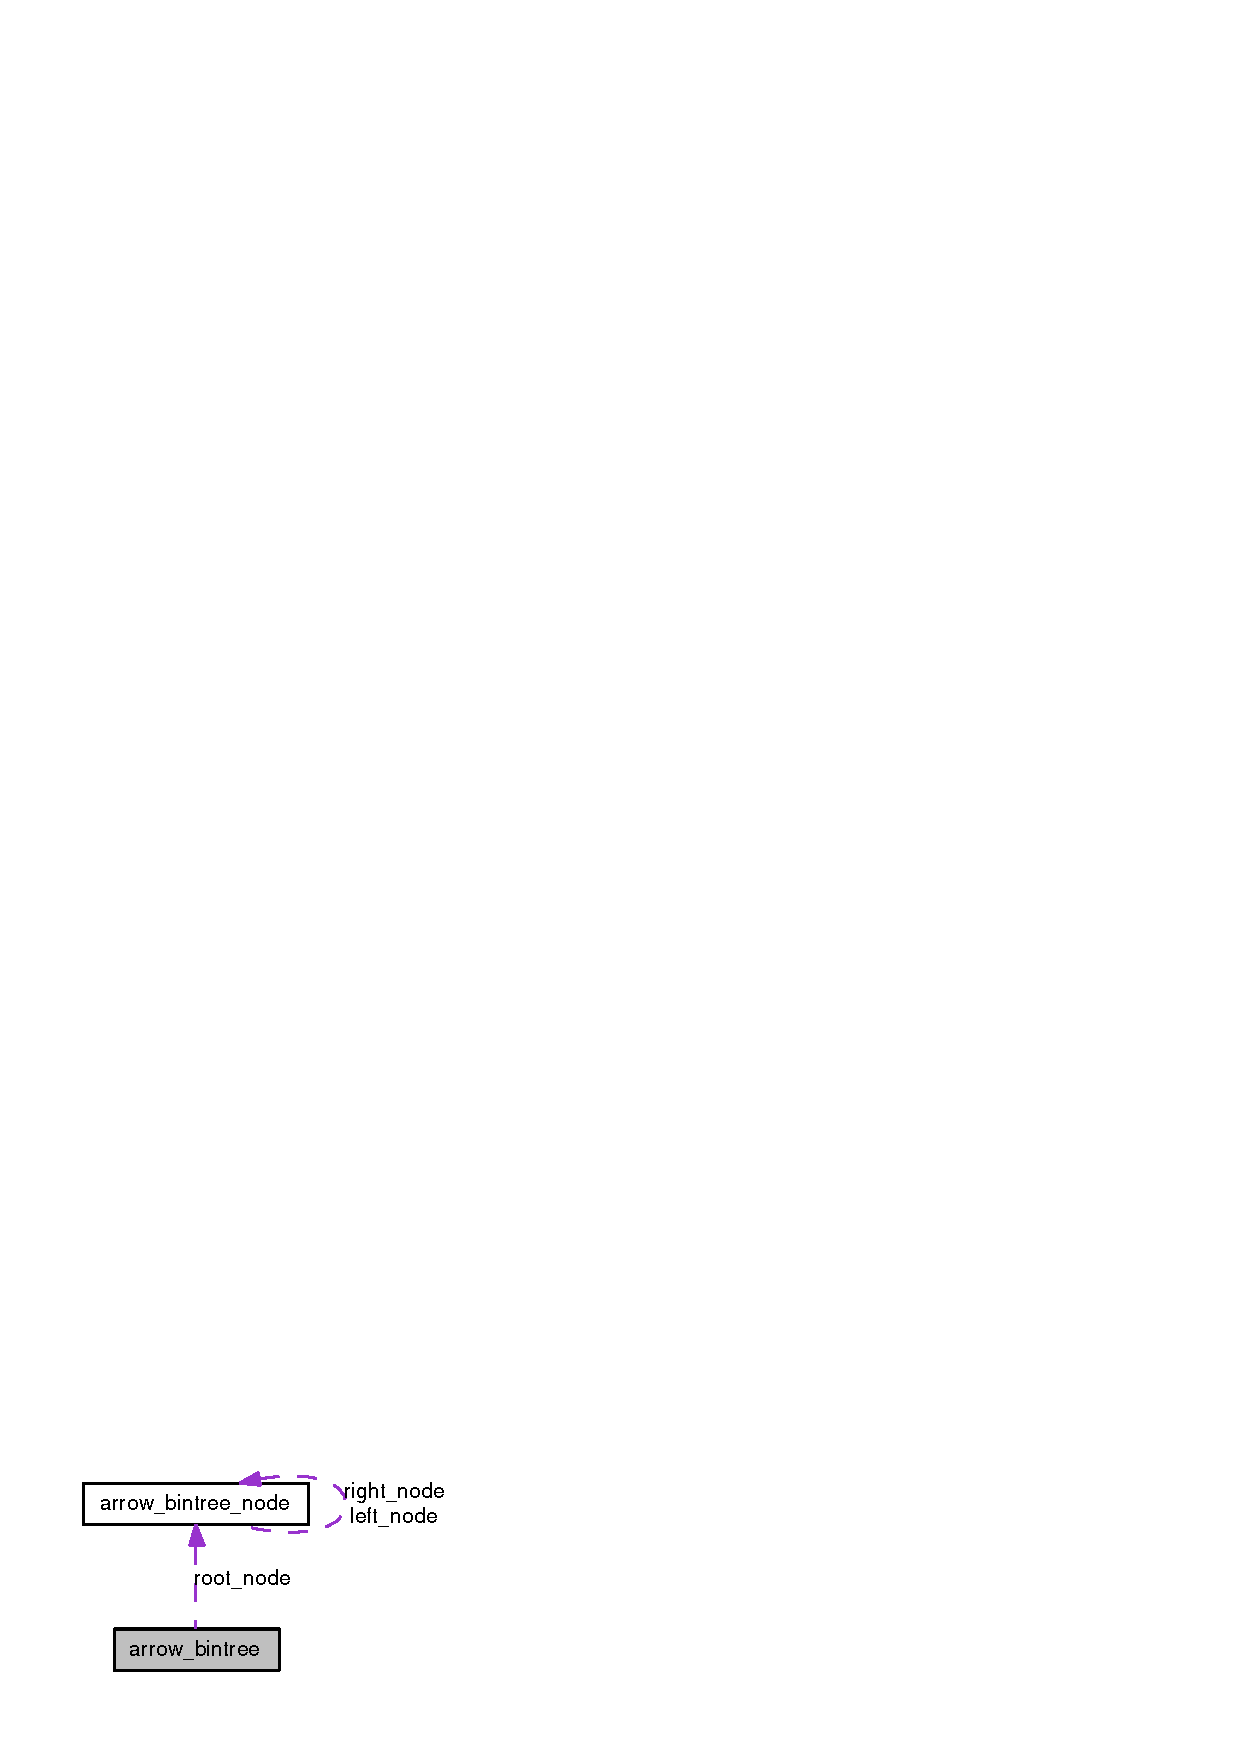
\includegraphics[width=109pt]{structarrow__bintree__coll__graph}
\end{center}
\end{figure}
\subsection*{Data Fields}
\begin{CompactItemize}
\item 
struct \hyperlink{structarrow__bintree__node}{arrow\_\-bintree\_\-node} $\ast$ \hyperlink{structarrow__bintree_09f6d0bd6e32ae2c2f8df57a31388df6}{root\_\-node}
\item 
int \hyperlink{structarrow__bintree_7570628df0b5317cc8e240499ba12974}{size}
\end{CompactItemize}


\subsection{Detailed Description}
Binary tree data structure. 

Definition at line 82 of file common.h.

\subsection{Field Documentation}
\hypertarget{structarrow__bintree_09f6d0bd6e32ae2c2f8df57a31388df6}{
\index{arrow\_\-bintree@{arrow\_\-bintree}!root\_\-node@{root\_\-node}}
\index{root\_\-node@{root\_\-node}!arrow_bintree@{arrow\_\-bintree}}
\subsubsection{\setlength{\rightskip}{0pt plus 5cm}struct {\bf arrow\_\-bintree\_\-node}$\ast$ {\bf arrow\_\-bintree::root\_\-node}\hspace{0.3cm}{\tt  \mbox{[}read\mbox{]}}}}
\label{structarrow__bintree_09f6d0bd6e32ae2c2f8df57a31388df6}


root node of tree 

Definition at line 84 of file common.h.

Referenced by arrow\_\-bintree\_\-destruct(), arrow\_\-bintree\_\-init(), arrow\_\-bintree\_\-insert(), and arrow\_\-bintree\_\-to\_\-array().\hypertarget{structarrow__bintree_7570628df0b5317cc8e240499ba12974}{
\index{arrow\_\-bintree@{arrow\_\-bintree}!size@{size}}
\index{size@{size}!arrow_bintree@{arrow\_\-bintree}}
\subsubsection{\setlength{\rightskip}{0pt plus 5cm}int {\bf arrow\_\-bintree::size}}}
\label{structarrow__bintree_7570628df0b5317cc8e240499ba12974}


size of tree 

Definition at line 85 of file common.h.

Referenced by arrow\_\-bintree\_\-destruct(), arrow\_\-bintree\_\-init(), arrow\_\-bintree\_\-insert(), arrow\_\-bintree\_\-to\_\-new\_\-array(), arrow\_\-problem\_\-info\_\-get(), and insert\_\-at().

The documentation for this struct was generated from the following file:\begin{CompactItemize}
\item 
include/\hyperlink{common_8h}{common.h}\end{CompactItemize}

\hypertarget{structarrow__bintree__node}{
\section{arrow\_\-bintree\_\-node Struct Reference}
\label{structarrow__bintree__node}\index{arrow\_\-bintree\_\-node@{arrow\_\-bintree\_\-node}}
}
Binary tree node.  


{\tt \#include $<$arrow.h$>$}

Collaboration diagram for arrow\_\-bintree\_\-node:\nopagebreak
\begin{figure}[H]
\begin{center}
\leavevmode
\includegraphics[width=109pt]{structarrow__bintree__node__coll__graph}
\end{center}
\end{figure}
\subsection*{Data Fields}
\begin{CompactItemize}
\item 
int \hyperlink{structarrow__bintree__node_de01c6e7aa823db027836d77e7ce48b6}{data}
\item 
int \hyperlink{structarrow__bintree__node_a359d3d029023fb8763af3329207ee53}{has\_\-left\_\-node}
\item 
int \hyperlink{structarrow__bintree__node_f6f8bb35c520a88841a810777e9bc186}{has\_\-right\_\-node}
\item 
struct \hyperlink{structarrow__bintree__node}{arrow\_\-bintree\_\-node} $\ast$ \hyperlink{structarrow__bintree__node_e7eb125cad02704a57796b16c49b2983}{left\_\-node}
\item 
struct \hyperlink{structarrow__bintree__node}{arrow\_\-bintree\_\-node} $\ast$ \hyperlink{structarrow__bintree__node_4875801983f2b0220212951e6c0130af}{right\_\-node}
\end{CompactItemize}


\subsection{Detailed Description}
Binary tree node. 

Definition at line 97 of file arrow.h.

\subsection{Field Documentation}
\hypertarget{structarrow__bintree__node_de01c6e7aa823db027836d77e7ce48b6}{
\index{arrow\_\-bintree\_\-node@{arrow\_\-bintree\_\-node}!data@{data}}
\index{data@{data}!arrow_bintree_node@{arrow\_\-bintree\_\-node}}
\subsubsection{\setlength{\rightskip}{0pt plus 5cm}int {\bf arrow\_\-bintree\_\-node::data}}}
\label{structarrow__bintree__node_de01c6e7aa823db027836d77e7ce48b6}


data contained in node 

Definition at line 99 of file arrow.h.

Referenced by fill\_\-array(), and insert\_\-at().\hypertarget{structarrow__bintree__node_a359d3d029023fb8763af3329207ee53}{
\index{arrow\_\-bintree\_\-node@{arrow\_\-bintree\_\-node}!has\_\-left\_\-node@{has\_\-left\_\-node}}
\index{has\_\-left\_\-node@{has\_\-left\_\-node}!arrow_bintree_node@{arrow\_\-bintree\_\-node}}
\subsubsection{\setlength{\rightskip}{0pt plus 5cm}int {\bf arrow\_\-bintree\_\-node::has\_\-left\_\-node}}}
\label{structarrow__bintree__node_a359d3d029023fb8763af3329207ee53}


true if left node exists 

Definition at line 100 of file arrow.h.

Referenced by destruct\_\-node(), fill\_\-array(), and insert\_\-at().\hypertarget{structarrow__bintree__node_f6f8bb35c520a88841a810777e9bc186}{
\index{arrow\_\-bintree\_\-node@{arrow\_\-bintree\_\-node}!has\_\-right\_\-node@{has\_\-right\_\-node}}
\index{has\_\-right\_\-node@{has\_\-right\_\-node}!arrow_bintree_node@{arrow\_\-bintree\_\-node}}
\subsubsection{\setlength{\rightskip}{0pt plus 5cm}int {\bf arrow\_\-bintree\_\-node::has\_\-right\_\-node}}}
\label{structarrow__bintree__node_f6f8bb35c520a88841a810777e9bc186}


true if right node exists 

Definition at line 101 of file arrow.h.

Referenced by destruct\_\-node(), fill\_\-array(), and insert\_\-at().\hypertarget{structarrow__bintree__node_e7eb125cad02704a57796b16c49b2983}{
\index{arrow\_\-bintree\_\-node@{arrow\_\-bintree\_\-node}!left\_\-node@{left\_\-node}}
\index{left\_\-node@{left\_\-node}!arrow_bintree_node@{arrow\_\-bintree\_\-node}}
\subsubsection{\setlength{\rightskip}{0pt plus 5cm}struct {\bf arrow\_\-bintree\_\-node}$\ast$ {\bf arrow\_\-bintree\_\-node::left\_\-node}\hspace{0.3cm}{\tt  \mbox{[}read\mbox{]}}}}
\label{structarrow__bintree__node_e7eb125cad02704a57796b16c49b2983}


left node 

Definition at line 102 of file arrow.h.

Referenced by destruct\_\-node(), fill\_\-array(), and insert\_\-at().\hypertarget{structarrow__bintree__node_4875801983f2b0220212951e6c0130af}{
\index{arrow\_\-bintree\_\-node@{arrow\_\-bintree\_\-node}!right\_\-node@{right\_\-node}}
\index{right\_\-node@{right\_\-node}!arrow_bintree_node@{arrow\_\-bintree\_\-node}}
\subsubsection{\setlength{\rightskip}{0pt plus 5cm}struct {\bf arrow\_\-bintree\_\-node}$\ast$ {\bf arrow\_\-bintree\_\-node::right\_\-node}\hspace{0.3cm}{\tt  \mbox{[}read\mbox{]}}}}
\label{structarrow__bintree__node_4875801983f2b0220212951e6c0130af}


right node 

Definition at line 103 of file arrow.h.

Referenced by destruct\_\-node(), fill\_\-array(), and insert\_\-at().

The documentation for this struct was generated from the following file:\begin{CompactItemize}
\item 
lib/\hyperlink{arrow_8h}{arrow.h}\end{CompactItemize}

\hypertarget{structarrow__bound__result}{
\section{arrow\_\-bound\_\-result Struct Reference}
\label{structarrow__bound__result}\index{arrow\_\-bound\_\-result@{arrow\_\-bound\_\-result}}
}
A lower bound result.  


{\tt \#include $<$lb.h$>$}

\subsection*{Data Fields}
\begin{CompactItemize}
\item 
int \hyperlink{structarrow__bound__result_acbca68de984376a60dbb9893935e0f4}{obj\_\-value}
\item 
double \hyperlink{structarrow__bound__result_d27a3cae43bbe1ed2e2c60a4ef307b08}{total\_\-time}
\end{CompactItemize}


\subsection{Detailed Description}
A lower bound result. 

Definition at line 21 of file lb.h.

\subsection{Field Documentation}
\hypertarget{structarrow__bound__result_acbca68de984376a60dbb9893935e0f4}{
\index{arrow\_\-bound\_\-result@{arrow\_\-bound\_\-result}!obj\_\-value@{obj\_\-value}}
\index{obj\_\-value@{obj\_\-value}!arrow_bound_result@{arrow\_\-bound\_\-result}}
\subsubsection[{obj\_\-value}]{\setlength{\rightskip}{0pt plus 5cm}int {\bf arrow\_\-bound\_\-result::obj\_\-value}}}
\label{structarrow__bound__result_acbca68de984376a60dbb9893935e0f4}


objective value 

Definition at line 23 of file lb.h.

Referenced by arrow\_\-2mb\_\-solve(), arrow\_\-bap\_\-solve(), arrow\_\-bbssp\_\-solve(), arrow\_\-bscssp\_\-solve(), arrow\_\-cbap\_\-solve(), arrow\_\-cbst\_\-solve(), arrow\_\-dcbpb\_\-solve(), and main().\hypertarget{structarrow__bound__result_d27a3cae43bbe1ed2e2c60a4ef307b08}{
\index{arrow\_\-bound\_\-result@{arrow\_\-bound\_\-result}!total\_\-time@{total\_\-time}}
\index{total\_\-time@{total\_\-time}!arrow_bound_result@{arrow\_\-bound\_\-result}}
\subsubsection[{total\_\-time}]{\setlength{\rightskip}{0pt plus 5cm}double {\bf arrow\_\-bound\_\-result::total\_\-time}}}
\label{structarrow__bound__result_d27a3cae43bbe1ed2e2c60a4ef307b08}


total time 

Definition at line 24 of file lb.h.

Referenced by arrow\_\-2mb\_\-solve(), arrow\_\-bap\_\-solve(), arrow\_\-bbssp\_\-solve(), arrow\_\-bscssp\_\-solve(), arrow\_\-cbap\_\-solve(), arrow\_\-cbst\_\-solve(), arrow\_\-dcbpb\_\-solve(), and main().

The documentation for this struct was generated from the following file:\begin{CompactItemize}
\item 
include/\hyperlink{lb_8h}{lb.h}\end{CompactItemize}

\hypertarget{structarrow__btsp__fun}{
\section{arrow\_\-btsp\_\-fun Struct Reference}
\label{structarrow__btsp__fun}\index{arrow\_\-btsp\_\-fun@{arrow\_\-btsp\_\-fun}}
}
BTSP Cost matrix function definition.  


{\tt \#include $<$btsp.h$>$}

\subsection*{Data Fields}
\begin{CompactItemize}
\item 
void $\ast$ \hyperlink{structarrow__btsp__fun_9c1a276685fb0cac372faef2dd2ba99a}{data}
\item 
int \hyperlink{structarrow__btsp__fun_1950686e4862a4b1bd68d1ada85e2c79}{shallow}
\item 
int($\ast$ \hyperlink{structarrow__btsp__fun_ffc634f9d1a545f890b0b2007aff544d}{get\_\-cost} )(struct \hyperlink{structarrow__btsp__fun}{arrow\_\-btsp\_\-fun} $\ast$fun, \hyperlink{structarrow__problem}{arrow\_\-problem} $\ast$base\_\-problem, int min\_\-cost, int max\_\-cost, int i, int j)
\begin{CompactList}\small\item\em Retrieves cost between nodes i and j from the function. \item\end{CompactList}\item 
int($\ast$ \hyperlink{structarrow__btsp__fun_c588686921bd526653a7e0d7816aee44}{initialize} )(struct \hyperlink{structarrow__btsp__fun}{arrow\_\-btsp\_\-fun} $\ast$fun)
\begin{CompactList}\small\item\em Initializes the function structure for a new problem. \item\end{CompactList}\item 
void($\ast$ \hyperlink{structarrow__btsp__fun_6c66b7591252728aaa441139c623446a}{destruct} )(struct \hyperlink{structarrow__btsp__fun}{arrow\_\-btsp\_\-fun} $\ast$fun)
\begin{CompactList}\small\item\em Destructs the function structure. \item\end{CompactList}\item 
int($\ast$ \hyperlink{structarrow__btsp__fun_98369e55806c13b3ba90c8c1cbe1f8a4}{feasible} )(struct \hyperlink{structarrow__btsp__fun}{arrow\_\-btsp\_\-fun} $\ast$fun, \hyperlink{structarrow__problem}{arrow\_\-problem} $\ast$base\_\-problem, int min\_\-cost, int max\_\-cost, double tour\_\-length, int $\ast$tour)
\begin{CompactList}\small\item\em Determines if the given tour is feasible or not. \item\end{CompactList}\end{CompactItemize}


\subsection{Detailed Description}
BTSP Cost matrix function definition. 

Definition at line 44 of file btsp.h.

\subsection{Field Documentation}
\hypertarget{structarrow__btsp__fun_9c1a276685fb0cac372faef2dd2ba99a}{
\index{arrow\_\-btsp\_\-fun@{arrow\_\-btsp\_\-fun}!data@{data}}
\index{data@{data}!arrow_btsp_fun@{arrow\_\-btsp\_\-fun}}
\subsubsection[{data}]{\setlength{\rightskip}{0pt plus 5cm}void$\ast$ {\bf arrow\_\-btsp\_\-fun::data}}}
\label{structarrow__btsp__fun_9c1a276685fb0cac372faef2dd2ba99a}


data required by function 

Definition at line 46 of file btsp.h.

Referenced by arrow\_\-baltsp\_\-fun\_\-basic(), arrow\_\-baltsp\_\-fun\_\-dt2(), arrow\_\-baltsp\_\-fun\_\-ib(), arrow\_\-baltsp\_\-fun\_\-shake(), arrow\_\-baltsp\_\-fun\_\-ut(), arrow\_\-btsp\_\-fun\_\-asym\_\-shift(), arrow\_\-btsp\_\-fun\_\-basic(), arrow\_\-btsp\_\-fun\_\-cbtsp\_\-basic(), arrow\_\-btsp\_\-fun\_\-cbtsp\_\-shake(), arrow\_\-btsp\_\-fun\_\-shake\_\-1(), baltsp\_\-dt2\_\-feasible(), baltsp\_\-dt2\_\-get\_\-cost(), baltsp\_\-dt2\_\-initialize(), baltsp\_\-shake\_\-destruct(), baltsp\_\-shake\_\-get\_\-cost(), baltsp\_\-shake\_\-initialize(), btsp\_\-asym\_\-shift\_\-destruct(), btsp\_\-asym\_\-shift\_\-feasible(), btsp\_\-asym\_\-shift\_\-get\_\-cost(), btsp\_\-shake\_\-1\_\-destruct(), btsp\_\-shake\_\-1\_\-get\_\-cost(), btsp\_\-shake\_\-1\_\-initialize(), cbtsp\_\-basic\_\-destruct(), cbtsp\_\-basic\_\-feasible(), cbtsp\_\-basic\_\-get\_\-cost(), cbtsp\_\-shake\_\-destruct(), cbtsp\_\-shake\_\-feasible(), cbtsp\_\-shake\_\-get\_\-cost(), and cbtsp\_\-shake\_\-initialize().\hypertarget{structarrow__btsp__fun_6c66b7591252728aaa441139c623446a}{
\index{arrow\_\-btsp\_\-fun@{arrow\_\-btsp\_\-fun}!destruct@{destruct}}
\index{destruct@{destruct}!arrow_btsp_fun@{arrow\_\-btsp\_\-fun}}
\subsubsection[{destruct}]{\setlength{\rightskip}{0pt plus 5cm}void($\ast$ {\bf arrow\_\-btsp\_\-fun::destruct})(struct {\bf arrow\_\-btsp\_\-fun} $\ast$fun)}}
\label{structarrow__btsp__fun_6c66b7591252728aaa441139c623446a}


Destructs the function structure. 

\begin{Desc}
\item[Parameters:]
\begin{description}
\item[{\em fun}]\mbox{[}out\mbox{]} function structure \end{description}
\end{Desc}


Referenced by arrow\_\-baltsp\_\-fun\_\-basic(), arrow\_\-baltsp\_\-fun\_\-dt2(), arrow\_\-baltsp\_\-fun\_\-ib(), arrow\_\-baltsp\_\-fun\_\-shake(), arrow\_\-baltsp\_\-fun\_\-ut(), arrow\_\-btsp\_\-fun\_\-asym\_\-shift(), arrow\_\-btsp\_\-fun\_\-basic(), arrow\_\-btsp\_\-fun\_\-cbtsp\_\-basic(), arrow\_\-btsp\_\-fun\_\-cbtsp\_\-shake(), arrow\_\-btsp\_\-fun\_\-destruct(), and arrow\_\-btsp\_\-fun\_\-shake\_\-1().\hypertarget{structarrow__btsp__fun_98369e55806c13b3ba90c8c1cbe1f8a4}{
\index{arrow\_\-btsp\_\-fun@{arrow\_\-btsp\_\-fun}!feasible@{feasible}}
\index{feasible@{feasible}!arrow_btsp_fun@{arrow\_\-btsp\_\-fun}}
\subsubsection[{feasible}]{\setlength{\rightskip}{0pt plus 5cm}int($\ast$ {\bf arrow\_\-btsp\_\-fun::feasible})(struct {\bf arrow\_\-btsp\_\-fun} $\ast$fun, {\bf arrow\_\-problem} $\ast$base\_\-problem, int min\_\-cost, int max\_\-cost, double tour\_\-length, int $\ast$tour)}}
\label{structarrow__btsp__fun_98369e55806c13b3ba90c8c1cbe1f8a4}


Determines if the given tour is feasible or not. 

\begin{Desc}
\item[Parameters:]
\begin{description}
\item[{\em fun}]\mbox{[}in\mbox{]} function structure \item[{\em problem}]\mbox{[}in\mbox{]} the problem to check against \item[{\em min\_\-cost}]\mbox{[}in\mbox{]} min\_\-cost to consider for active edges \item[{\em max\_\-cost}]\mbox{[}in\mbox{]} max\_\-cost to consider for active edges \item[{\em tour\_\-length}]\mbox{[}in\mbox{]} the length of the given tour \item[{\em tour}]\mbox{[}in\mbox{]} the tour in node-node format \end{description}
\end{Desc}
\begin{Desc}
\item[Returns:]ARROW\_\-TRUE if the tour is feasible, ARROW\_\-FALSE if not \end{Desc}


Referenced by arrow\_\-baltsp\_\-fun\_\-basic(), arrow\_\-baltsp\_\-fun\_\-dt2(), arrow\_\-baltsp\_\-fun\_\-ib(), arrow\_\-baltsp\_\-fun\_\-shake(), arrow\_\-baltsp\_\-fun\_\-ut(), arrow\_\-btsp\_\-feasible(), arrow\_\-btsp\_\-fun\_\-asym\_\-shift(), arrow\_\-btsp\_\-fun\_\-basic(), arrow\_\-btsp\_\-fun\_\-cbtsp\_\-basic(), arrow\_\-btsp\_\-fun\_\-cbtsp\_\-shake(), and arrow\_\-btsp\_\-fun\_\-shake\_\-1().\hypertarget{structarrow__btsp__fun_ffc634f9d1a545f890b0b2007aff544d}{
\index{arrow\_\-btsp\_\-fun@{arrow\_\-btsp\_\-fun}!get\_\-cost@{get\_\-cost}}
\index{get\_\-cost@{get\_\-cost}!arrow_btsp_fun@{arrow\_\-btsp\_\-fun}}
\subsubsection[{get\_\-cost}]{\setlength{\rightskip}{0pt plus 5cm}int($\ast$ {\bf arrow\_\-btsp\_\-fun::get\_\-cost})(struct {\bf arrow\_\-btsp\_\-fun} $\ast$fun, {\bf arrow\_\-problem} $\ast$base\_\-problem, int min\_\-cost, int max\_\-cost, int i, int j)}}
\label{structarrow__btsp__fun_ffc634f9d1a545f890b0b2007aff544d}


Retrieves cost between nodes i and j from the function. 

\begin{Desc}
\item[Parameters:]
\begin{description}
\item[{\em fun}]\mbox{[}in\mbox{]} function structure \item[{\em problem}]\mbox{[}in\mbox{]} problem structure \item[{\em min\_\-cost}]\mbox{[}in\mbox{]} min\_\-cost to consider for active edges \item[{\em max\_\-cost}]\mbox{[}in\mbox{]} max\_\-cost to consider for active edges \item[{\em i}]\mbox{[}in\mbox{]} id of start node \item[{\em j}]\mbox{[}in\mbox{]} id of end node \end{description}
\end{Desc}
\begin{Desc}
\item[Returns:]cost between node i and node j \end{Desc}


Referenced by apply\_\-deep(), arrow\_\-baltsp\_\-fun\_\-basic(), arrow\_\-baltsp\_\-fun\_\-dt2(), arrow\_\-baltsp\_\-fun\_\-ib(), arrow\_\-baltsp\_\-fun\_\-shake(), arrow\_\-baltsp\_\-fun\_\-ut(), arrow\_\-btsp\_\-fun\_\-asym\_\-shift(), arrow\_\-btsp\_\-fun\_\-basic(), arrow\_\-btsp\_\-fun\_\-cbtsp\_\-basic(), arrow\_\-btsp\_\-fun\_\-cbtsp\_\-shake(), arrow\_\-btsp\_\-fun\_\-shake\_\-1(), and fun\_\-get\_\-cost().\hypertarget{structarrow__btsp__fun_c588686921bd526653a7e0d7816aee44}{
\index{arrow\_\-btsp\_\-fun@{arrow\_\-btsp\_\-fun}!initialize@{initialize}}
\index{initialize@{initialize}!arrow_btsp_fun@{arrow\_\-btsp\_\-fun}}
\subsubsection[{initialize}]{\setlength{\rightskip}{0pt plus 5cm}int($\ast$ {\bf arrow\_\-btsp\_\-fun::initialize})(struct {\bf arrow\_\-btsp\_\-fun} $\ast$fun)}}
\label{structarrow__btsp__fun_c588686921bd526653a7e0d7816aee44}


Initializes the function structure for a new problem. 

\begin{Desc}
\item[Parameters:]
\begin{description}
\item[{\em fun}]\mbox{[}out\mbox{]} function structure \end{description}
\end{Desc}


Referenced by arrow\_\-baltsp\_\-fun\_\-basic(), arrow\_\-baltsp\_\-fun\_\-dt2(), arrow\_\-baltsp\_\-fun\_\-ib(), arrow\_\-baltsp\_\-fun\_\-shake(), arrow\_\-baltsp\_\-fun\_\-ut(), arrow\_\-btsp\_\-fun\_\-apply(), arrow\_\-btsp\_\-fun\_\-asym\_\-shift(), arrow\_\-btsp\_\-fun\_\-basic(), arrow\_\-btsp\_\-fun\_\-cbtsp\_\-basic(), arrow\_\-btsp\_\-fun\_\-cbtsp\_\-shake(), and arrow\_\-btsp\_\-fun\_\-shake\_\-1().\hypertarget{structarrow__btsp__fun_1950686e4862a4b1bd68d1ada85e2c79}{
\index{arrow\_\-btsp\_\-fun@{arrow\_\-btsp\_\-fun}!shallow@{shallow}}
\index{shallow@{shallow}!arrow_btsp_fun@{arrow\_\-btsp\_\-fun}}
\subsubsection[{shallow}]{\setlength{\rightskip}{0pt plus 5cm}int {\bf arrow\_\-btsp\_\-fun::shallow}}}
\label{structarrow__btsp__fun_1950686e4862a4b1bd68d1ada85e2c79}


indicates use of shallow copy of data 

Definition at line 47 of file btsp.h.

Referenced by arrow\_\-baltsp\_\-fun\_\-basic(), arrow\_\-baltsp\_\-fun\_\-dt2(), arrow\_\-baltsp\_\-fun\_\-ib(), arrow\_\-baltsp\_\-fun\_\-shake(), arrow\_\-baltsp\_\-fun\_\-ut(), arrow\_\-btsp\_\-fun\_\-apply(), arrow\_\-btsp\_\-fun\_\-asym\_\-shift(), arrow\_\-btsp\_\-fun\_\-basic(), arrow\_\-btsp\_\-fun\_\-cbtsp\_\-basic(), arrow\_\-btsp\_\-fun\_\-cbtsp\_\-shake(), and arrow\_\-btsp\_\-fun\_\-shake\_\-1().

The documentation for this struct was generated from the following file:\begin{CompactItemize}
\item 
include/\hyperlink{btsp_8h}{btsp.h}\end{CompactItemize}

\hypertarget{structarrow__btsp__params}{
\section{arrow\_\-btsp\_\-params Struct Reference}
\label{structarrow__btsp__params}\index{arrow\_\-btsp\_\-params@{arrow\_\-btsp\_\-params}}
}
BTSP algorithm parameters.  


{\tt \#include $<$arrow.h$>$}

Collaboration diagram for arrow\_\-btsp\_\-params:\subsection*{Data Fields}
\begin{CompactItemize}
\item 
int \hyperlink{structarrow__btsp__params_2c579feb3ff41f4d73b5de97596fe465}{confirm\_\-sol}
\item 
int \hyperlink{structarrow__btsp__params_cd85b850ac7c8495a4689100e8c3182c}{supress\_\-ebst}
\item 
int \hyperlink{structarrow__btsp__params_f5fd677200b64930838c6905cbada990}{find\_\-short\_\-tour}
\item 
int \hyperlink{structarrow__btsp__params_da747e3797f9327834e4dbb1459d2786}{lower\_\-bound}
\item 
int \hyperlink{structarrow__btsp__params_b8749004215015a78139b8e4e1fb8905}{upper\_\-bound}
\item 
int \hyperlink{structarrow__btsp__params_2897d24f2fdd53c723609cf68880f55e}{num\_\-steps}
\item 
\hyperlink{structarrow__btsp__solve__plan}{arrow\_\-btsp\_\-solve\_\-plan} $\ast$ \hyperlink{structarrow__btsp__params_49aedb95b2fc4a725e3bb8485470484b}{steps}
\end{CompactItemize}


\subsection{Detailed Description}
BTSP algorithm parameters. 

Definition at line 241 of file arrow.h.

\subsection{Field Documentation}
\hypertarget{structarrow__btsp__params_2c579feb3ff41f4d73b5de97596fe465}{
\index{arrow\_\-btsp\_\-params@{arrow\_\-btsp\_\-params}!confirm\_\-sol@{confirm\_\-sol}}
\index{confirm\_\-sol@{confirm\_\-sol}!arrow_btsp_params@{arrow\_\-btsp\_\-params}}
\subsubsection{\setlength{\rightskip}{0pt plus 5cm}int {\bf arrow\_\-btsp\_\-params::confirm\_\-sol}}}
\label{structarrow__btsp__params_2c579feb3ff41f4d73b5de97596fe465}


confirm sol. with exact solver? 

Definition at line 243 of file arrow.h.

Referenced by arrow\_\-btsp\_\-params\_\-init(), arrow\_\-btsp\_\-solve(), and main().\hypertarget{structarrow__btsp__params_cd85b850ac7c8495a4689100e8c3182c}{
\index{arrow\_\-btsp\_\-params@{arrow\_\-btsp\_\-params}!supress\_\-ebst@{supress\_\-ebst}}
\index{supress\_\-ebst@{supress\_\-ebst}!arrow_btsp_params@{arrow\_\-btsp\_\-params}}
\subsubsection{\setlength{\rightskip}{0pt plus 5cm}int {\bf arrow\_\-btsp\_\-params::supress\_\-ebst}}}
\label{structarrow__btsp__params_cd85b850ac7c8495a4689100e8c3182c}


supress EBST-heuristic? 

Definition at line 244 of file arrow.h.

Referenced by arrow\_\-btsp\_\-params\_\-init(), arrow\_\-btsp\_\-solve(), and main().\hypertarget{structarrow__btsp__params_f5fd677200b64930838c6905cbada990}{
\index{arrow\_\-btsp\_\-params@{arrow\_\-btsp\_\-params}!find\_\-short\_\-tour@{find\_\-short\_\-tour}}
\index{find\_\-short\_\-tour@{find\_\-short\_\-tour}!arrow_btsp_params@{arrow\_\-btsp\_\-params}}
\subsubsection{\setlength{\rightskip}{0pt plus 5cm}int {\bf arrow\_\-btsp\_\-params::find\_\-short\_\-tour}}}
\label{structarrow__btsp__params_f5fd677200b64930838c6905cbada990}


find short BSTP tour? 

Definition at line 245 of file arrow.h.

Referenced by arrow\_\-btsp\_\-params\_\-init(), arrow\_\-btsp\_\-solve(), and main().\hypertarget{structarrow__btsp__params_da747e3797f9327834e4dbb1459d2786}{
\index{arrow\_\-btsp\_\-params@{arrow\_\-btsp\_\-params}!lower\_\-bound@{lower\_\-bound}}
\index{lower\_\-bound@{lower\_\-bound}!arrow_btsp_params@{arrow\_\-btsp\_\-params}}
\subsubsection{\setlength{\rightskip}{0pt plus 5cm}int {\bf arrow\_\-btsp\_\-params::lower\_\-bound}}}
\label{structarrow__btsp__params_da747e3797f9327834e4dbb1459d2786}


initial lower bound 

Definition at line 246 of file arrow.h.

Referenced by arrow\_\-btsp\_\-params\_\-init(), arrow\_\-btsp\_\-solve(), and main().\hypertarget{structarrow__btsp__params_b8749004215015a78139b8e4e1fb8905}{
\index{arrow\_\-btsp\_\-params@{arrow\_\-btsp\_\-params}!upper\_\-bound@{upper\_\-bound}}
\index{upper\_\-bound@{upper\_\-bound}!arrow_btsp_params@{arrow\_\-btsp\_\-params}}
\subsubsection{\setlength{\rightskip}{0pt plus 5cm}int {\bf arrow\_\-btsp\_\-params::upper\_\-bound}}}
\label{structarrow__btsp__params_b8749004215015a78139b8e4e1fb8905}


initial upper bound 

Definition at line 247 of file arrow.h.

Referenced by arrow\_\-btsp\_\-params\_\-init(), arrow\_\-btsp\_\-solve(), and main().\hypertarget{structarrow__btsp__params_2897d24f2fdd53c723609cf68880f55e}{
\index{arrow\_\-btsp\_\-params@{arrow\_\-btsp\_\-params}!num\_\-steps@{num\_\-steps}}
\index{num\_\-steps@{num\_\-steps}!arrow_btsp_params@{arrow\_\-btsp\_\-params}}
\subsubsection{\setlength{\rightskip}{0pt plus 5cm}int {\bf arrow\_\-btsp\_\-params::num\_\-steps}}}
\label{structarrow__btsp__params_2897d24f2fdd53c723609cf68880f55e}


the number of solve plan steps 

Definition at line 248 of file arrow.h.

Referenced by arrow\_\-btsp\_\-params\_\-destruct(), arrow\_\-btsp\_\-params\_\-init(), arrow\_\-btsp\_\-solve(), and main().\hypertarget{structarrow__btsp__params_49aedb95b2fc4a725e3bb8485470484b}{
\index{arrow\_\-btsp\_\-params@{arrow\_\-btsp\_\-params}!steps@{steps}}
\index{steps@{steps}!arrow_btsp_params@{arrow\_\-btsp\_\-params}}
\subsubsection{\setlength{\rightskip}{0pt plus 5cm}{\bf arrow\_\-btsp\_\-solve\_\-plan}$\ast$ {\bf arrow\_\-btsp\_\-params::steps}}}
\label{structarrow__btsp__params_49aedb95b2fc4a725e3bb8485470484b}


solve plan steps 

Definition at line 249 of file arrow.h.

Referenced by arrow\_\-btsp\_\-params\_\-destruct(), arrow\_\-btsp\_\-solve(), and main().

The documentation for this struct was generated from the following file:\begin{CompactItemize}
\item 
lib/\hyperlink{arrow_8h}{arrow.h}\end{CompactItemize}

\hypertarget{structarrow__btsp__result}{
\section{arrow\_\-btsp\_\-result Struct Reference}
\label{structarrow__btsp__result}\index{arrow\_\-btsp\_\-result@{arrow\_\-btsp\_\-result}}
}
BTSP result.  


{\tt \#include $<$arrow.h$>$}

\subsection*{Data Fields}
\begin{CompactItemize}
\item 
int \hyperlink{structarrow__btsp__result_6ba21b4231cfe2c1e437a9f7e8f31aa6}{found\_\-tour}
\item 
int \hyperlink{structarrow__btsp__result_ea5f7f45bf61f33ca6b57829da92e041}{obj\_\-value}
\item 
double \hyperlink{structarrow__btsp__result_3c0b8827a873df71166e7fe9419c45c2}{tour\_\-length}
\item 
int $\ast$ \hyperlink{structarrow__btsp__result_ebd9a553dc3bf31f52eda0b293b0e272}{tour}
\item 
int \hyperlink{structarrow__btsp__result_febcf61e24bf277eeb7795c18bd42b8b}{optimal}
\item 
int \hyperlink{structarrow__btsp__result_80106c5f0b8f82353ad6771ad9eaac71}{bin\_\-search\_\-steps}
\item 
int \hyperlink{structarrow__btsp__result_53b6e6b7922eb5c3e5a1b135d42d5654}{linkern\_\-attempts}
\item 
double \hyperlink{structarrow__btsp__result_7e8a3ff6f55c89caa52a7a793fa36dd6}{linkern\_\-time}
\item 
int \hyperlink{structarrow__btsp__result_47433b850b6addae44522177a50696b3}{exact\_\-attempts}
\item 
double \hyperlink{structarrow__btsp__result_edefe82c06445f657e5147d52720bdef}{exact\_\-time}
\item 
double \hyperlink{structarrow__btsp__result_dea5711f0a574d98f66d1b20011a68de}{total\_\-time}
\end{CompactItemize}


\subsection{Detailed Description}
BTSP result. 

Definition at line 172 of file arrow.h.

\subsection{Field Documentation}
\hypertarget{structarrow__btsp__result_6ba21b4231cfe2c1e437a9f7e8f31aa6}{
\index{arrow\_\-btsp\_\-result@{arrow\_\-btsp\_\-result}!found\_\-tour@{found\_\-tour}}
\index{found\_\-tour@{found\_\-tour}!arrow_btsp_result@{arrow\_\-btsp\_\-result}}
\subsubsection{\setlength{\rightskip}{0pt plus 5cm}int {\bf arrow\_\-btsp\_\-result::found\_\-tour}}}
\label{structarrow__btsp__result_6ba21b4231cfe2c1e437a9f7e8f31aa6}


true if a tour was found, false otherwise 

Definition at line 174 of file arrow.h.

Referenced by arrow\_\-btsp\_\-result\_\-init(), arrow\_\-btsp\_\-solve(), feasible(), and main().\hypertarget{structarrow__btsp__result_ea5f7f45bf61f33ca6b57829da92e041}{
\index{arrow\_\-btsp\_\-result@{arrow\_\-btsp\_\-result}!obj\_\-value@{obj\_\-value}}
\index{obj\_\-value@{obj\_\-value}!arrow_btsp_result@{arrow\_\-btsp\_\-result}}
\subsubsection{\setlength{\rightskip}{0pt plus 5cm}int {\bf arrow\_\-btsp\_\-result::obj\_\-value}}}
\label{structarrow__btsp__result_ea5f7f45bf61f33ca6b57829da92e041}


objective value (largest cost in tour) 

Definition at line 175 of file arrow.h.

Referenced by arrow\_\-btsp\_\-result\_\-init(), arrow\_\-btsp\_\-solve(), feasible(), and main().\hypertarget{structarrow__btsp__result_3c0b8827a873df71166e7fe9419c45c2}{
\index{arrow\_\-btsp\_\-result@{arrow\_\-btsp\_\-result}!tour\_\-length@{tour\_\-length}}
\index{tour\_\-length@{tour\_\-length}!arrow_btsp_result@{arrow\_\-btsp\_\-result}}
\subsubsection{\setlength{\rightskip}{0pt plus 5cm}double {\bf arrow\_\-btsp\_\-result::tour\_\-length}}}
\label{structarrow__btsp__result_3c0b8827a873df71166e7fe9419c45c2}


length of the tour found 

Definition at line 176 of file arrow.h.

Referenced by arrow\_\-btsp\_\-result\_\-init(), arrow\_\-btsp\_\-solve(), feasible(), and main().\hypertarget{structarrow__btsp__result_ebd9a553dc3bf31f52eda0b293b0e272}{
\index{arrow\_\-btsp\_\-result@{arrow\_\-btsp\_\-result}!tour@{tour}}
\index{tour@{tour}!arrow_btsp_result@{arrow\_\-btsp\_\-result}}
\subsubsection{\setlength{\rightskip}{0pt plus 5cm}int$\ast$ {\bf arrow\_\-btsp\_\-result::tour}}}
\label{structarrow__btsp__result_ebd9a553dc3bf31f52eda0b293b0e272}


tour that was found in node-node format 

Definition at line 177 of file arrow.h.

Referenced by arrow\_\-btsp\_\-result\_\-destruct(), arrow\_\-btsp\_\-result\_\-init(), arrow\_\-btsp\_\-solve(), feasible(), and main().\hypertarget{structarrow__btsp__result_febcf61e24bf277eeb7795c18bd42b8b}{
\index{arrow\_\-btsp\_\-result@{arrow\_\-btsp\_\-result}!optimal@{optimal}}
\index{optimal@{optimal}!arrow_btsp_result@{arrow\_\-btsp\_\-result}}
\subsubsection{\setlength{\rightskip}{0pt plus 5cm}int {\bf arrow\_\-btsp\_\-result::optimal}}}
\label{structarrow__btsp__result_febcf61e24bf277eeb7795c18bd42b8b}


indicates if the solution is optimal 

Definition at line 178 of file arrow.h.

Referenced by arrow\_\-btsp\_\-solve(), and main().\hypertarget{structarrow__btsp__result_80106c5f0b8f82353ad6771ad9eaac71}{
\index{arrow\_\-btsp\_\-result@{arrow\_\-btsp\_\-result}!bin\_\-search\_\-steps@{bin\_\-search\_\-steps}}
\index{bin\_\-search\_\-steps@{bin\_\-search\_\-steps}!arrow_btsp_result@{arrow\_\-btsp\_\-result}}
\subsubsection{\setlength{\rightskip}{0pt plus 5cm}int {\bf arrow\_\-btsp\_\-result::bin\_\-search\_\-steps}}}
\label{structarrow__btsp__result_80106c5f0b8f82353ad6771ad9eaac71}


number of steps in binary search 

Definition at line 179 of file arrow.h.

Referenced by arrow\_\-btsp\_\-result\_\-init(), arrow\_\-btsp\_\-solve(), and main().\hypertarget{structarrow__btsp__result_53b6e6b7922eb5c3e5a1b135d42d5654}{
\index{arrow\_\-btsp\_\-result@{arrow\_\-btsp\_\-result}!linkern\_\-attempts@{linkern\_\-attempts}}
\index{linkern\_\-attempts@{linkern\_\-attempts}!arrow_btsp_result@{arrow\_\-btsp\_\-result}}
\subsubsection{\setlength{\rightskip}{0pt plus 5cm}int {\bf arrow\_\-btsp\_\-result::linkern\_\-attempts}}}
\label{structarrow__btsp__result_53b6e6b7922eb5c3e5a1b135d42d5654}


number of calls to LK heuristic 

Definition at line 180 of file arrow.h.

Referenced by arrow\_\-btsp\_\-result\_\-init(), arrow\_\-btsp\_\-solve(), feasible(), and main().\hypertarget{structarrow__btsp__result_7e8a3ff6f55c89caa52a7a793fa36dd6}{
\index{arrow\_\-btsp\_\-result@{arrow\_\-btsp\_\-result}!linkern\_\-time@{linkern\_\-time}}
\index{linkern\_\-time@{linkern\_\-time}!arrow_btsp_result@{arrow\_\-btsp\_\-result}}
\subsubsection{\setlength{\rightskip}{0pt plus 5cm}double {\bf arrow\_\-btsp\_\-result::linkern\_\-time}}}
\label{structarrow__btsp__result_7e8a3ff6f55c89caa52a7a793fa36dd6}


total time calling LK heuristic 

Definition at line 181 of file arrow.h.

Referenced by arrow\_\-btsp\_\-result\_\-init(), arrow\_\-btsp\_\-solve(), feasible(), and main().\hypertarget{structarrow__btsp__result_47433b850b6addae44522177a50696b3}{
\index{arrow\_\-btsp\_\-result@{arrow\_\-btsp\_\-result}!exact\_\-attempts@{exact\_\-attempts}}
\index{exact\_\-attempts@{exact\_\-attempts}!arrow_btsp_result@{arrow\_\-btsp\_\-result}}
\subsubsection{\setlength{\rightskip}{0pt plus 5cm}int {\bf arrow\_\-btsp\_\-result::exact\_\-attempts}}}
\label{structarrow__btsp__result_47433b850b6addae44522177a50696b3}


number of calls to exact TSP solver 

Definition at line 182 of file arrow.h.

Referenced by arrow\_\-btsp\_\-result\_\-init(), arrow\_\-btsp\_\-solve(), feasible(), and main().\hypertarget{structarrow__btsp__result_edefe82c06445f657e5147d52720bdef}{
\index{arrow\_\-btsp\_\-result@{arrow\_\-btsp\_\-result}!exact\_\-time@{exact\_\-time}}
\index{exact\_\-time@{exact\_\-time}!arrow_btsp_result@{arrow\_\-btsp\_\-result}}
\subsubsection{\setlength{\rightskip}{0pt plus 5cm}double {\bf arrow\_\-btsp\_\-result::exact\_\-time}}}
\label{structarrow__btsp__result_edefe82c06445f657e5147d52720bdef}


total time calling exact TSP solver 

Definition at line 183 of file arrow.h.

Referenced by arrow\_\-btsp\_\-result\_\-init(), arrow\_\-btsp\_\-solve(), feasible(), and main().\hypertarget{structarrow__btsp__result_dea5711f0a574d98f66d1b20011a68de}{
\index{arrow\_\-btsp\_\-result@{arrow\_\-btsp\_\-result}!total\_\-time@{total\_\-time}}
\index{total\_\-time@{total\_\-time}!arrow_btsp_result@{arrow\_\-btsp\_\-result}}
\subsubsection{\setlength{\rightskip}{0pt plus 5cm}double {\bf arrow\_\-btsp\_\-result::total\_\-time}}}
\label{structarrow__btsp__result_dea5711f0a574d98f66d1b20011a68de}


total time 

Definition at line 184 of file arrow.h.

Referenced by arrow\_\-btsp\_\-result\_\-init(), arrow\_\-btsp\_\-solve(), feasible(), and main().

The documentation for this struct was generated from the following file:\begin{CompactItemize}
\item 
lib/\hyperlink{arrow_8h}{arrow.h}\end{CompactItemize}

\hypertarget{structarrow__btsp__solve__plan}{
\section{arrow\_\-btsp\_\-solve\_\-plan Struct Reference}
\label{structarrow__btsp__solve__plan}\index{arrow\_\-btsp\_\-solve\_\-plan@{arrow\_\-btsp\_\-solve\_\-plan}}
}
BTSP feasibility solve step plan.  


{\tt \#include $<$btsp.h$>$}

Collaboration diagram for arrow\_\-btsp\_\-solve\_\-plan:\nopagebreak
\begin{figure}[H]
\begin{center}
\leavevmode
\includegraphics[width=136pt]{structarrow__btsp__solve__plan__coll__graph}
\end{center}
\end{figure}
\subsection*{Data Fields}
\begin{CompactItemize}
\item 
int \hyperlink{structarrow__btsp__solve__plan_911facf12673ddb5c3eb024fa12ee18d}{tsp\_\-solver}
\item 
void $\ast$ \hyperlink{structarrow__btsp__solve__plan_2b7cf65583f45c990218139dbae34ae5}{tsp\_\-params}
\item 
\hyperlink{structarrow__btsp__fun}{arrow\_\-btsp\_\-fun} \hyperlink{structarrow__btsp__solve__plan_89fa2ad1bcc026cd50fd7abc6c30ce3e}{fun}
\item 
int \hyperlink{structarrow__btsp__solve__plan_acfa3d4257a33548a9f60ee568219bc5}{attempts}
\end{CompactItemize}


\subsection{Detailed Description}
BTSP feasibility solve step plan. 

Definition at line 95 of file btsp.h.

\subsection{Field Documentation}
\hypertarget{structarrow__btsp__solve__plan_acfa3d4257a33548a9f60ee568219bc5}{
\index{arrow\_\-btsp\_\-solve\_\-plan@{arrow\_\-btsp\_\-solve\_\-plan}!attempts@{attempts}}
\index{attempts@{attempts}!arrow_btsp_solve_plan@{arrow\_\-btsp\_\-solve\_\-plan}}
\subsubsection[{attempts}]{\setlength{\rightskip}{0pt plus 5cm}int {\bf arrow\_\-btsp\_\-solve\_\-plan::attempts}}}
\label{structarrow__btsp__solve__plan_acfa3d4257a33548a9f60ee568219bc5}


number of attempts to perform 

Definition at line 100 of file btsp.h.

Referenced by arrow\_\-btsp\_\-feasible(), and arrow\_\-btsp\_\-solve\_\-plan\_\-init().\hypertarget{structarrow__btsp__solve__plan_89fa2ad1bcc026cd50fd7abc6c30ce3e}{
\index{arrow\_\-btsp\_\-solve\_\-plan@{arrow\_\-btsp\_\-solve\_\-plan}!fun@{fun}}
\index{fun@{fun}!arrow_btsp_solve_plan@{arrow\_\-btsp\_\-solve\_\-plan}}
\subsubsection[{fun}]{\setlength{\rightskip}{0pt plus 5cm}{\bf arrow\_\-btsp\_\-fun} {\bf arrow\_\-btsp\_\-solve\_\-plan::fun}}}
\label{structarrow__btsp__solve__plan_89fa2ad1bcc026cd50fd7abc6c30ce3e}


the cost matrix function to apply 

Definition at line 99 of file btsp.h.

Referenced by arrow\_\-btsp\_\-feasible(), and arrow\_\-btsp\_\-solve\_\-plan\_\-destruct().\hypertarget{structarrow__btsp__solve__plan_2b7cf65583f45c990218139dbae34ae5}{
\index{arrow\_\-btsp\_\-solve\_\-plan@{arrow\_\-btsp\_\-solve\_\-plan}!tsp\_\-params@{tsp\_\-params}}
\index{tsp\_\-params@{tsp\_\-params}!arrow_btsp_solve_plan@{arrow\_\-btsp\_\-solve\_\-plan}}
\subsubsection[{tsp\_\-params}]{\setlength{\rightskip}{0pt plus 5cm}void$\ast$ {\bf arrow\_\-btsp\_\-solve\_\-plan::tsp\_\-params}}}
\label{structarrow__btsp__solve__plan_2b7cf65583f45c990218139dbae34ae5}


TSP params to use 

Definition at line 98 of file btsp.h.

Referenced by arrow\_\-btsp\_\-feasible(), and arrow\_\-btsp\_\-solve\_\-plan\_\-destruct().\hypertarget{structarrow__btsp__solve__plan_911facf12673ddb5c3eb024fa12ee18d}{
\index{arrow\_\-btsp\_\-solve\_\-plan@{arrow\_\-btsp\_\-solve\_\-plan}!tsp\_\-solver@{tsp\_\-solver}}
\index{tsp\_\-solver@{tsp\_\-solver}!arrow_btsp_solve_plan@{arrow\_\-btsp\_\-solve\_\-plan}}
\subsubsection[{tsp\_\-solver}]{\setlength{\rightskip}{0pt plus 5cm}int {\bf arrow\_\-btsp\_\-solve\_\-plan::tsp\_\-solver}}}
\label{structarrow__btsp__solve__plan_911facf12673ddb5c3eb024fa12ee18d}


TSP solver to use 

Definition at line 97 of file btsp.h.

Referenced by arrow\_\-btsp\_\-feasible(), and arrow\_\-btsp\_\-solve\_\-plan\_\-destruct().

The documentation for this struct was generated from the following file:\begin{CompactItemize}
\item 
include/\hyperlink{btsp_8h}{btsp.h}\end{CompactItemize}

\hypertarget{structarrow__hash}{
\section{arrow\_\-hash Struct Reference}
\label{structarrow__hash}\index{arrow\_\-hash@{arrow\_\-hash}}
}
Hashtable.  


{\tt \#include $<$common.h$>$}

\subsection*{Data Fields}
\begin{CompactItemize}
\item 
cmph\_\-uint32 \hyperlink{structarrow__hash_f75ec1b9382f5b646007f8acb0521c15}{num\_\-keys}
\item 
char $\ast$$\ast$ \hyperlink{structarrow__hash_91eeed74d32d354b4e8b03be8b51f058}{vector}
\item 
char $\ast$ \hyperlink{structarrow__hash_298c5f151d99d62d6be200a620a4b4c3}{vector\_\-space}
\item 
cmph\_\-io\_\-adapter\_\-t $\ast$ \hyperlink{structarrow__hash_202a3f5b2689ae35543ef2c7ea84a6c2}{source}
\item 
cmph\_\-t $\ast$ \hyperlink{structarrow__hash_9f6c6f476d93187dd1436eac92bd8d53}{data}
\end{CompactItemize}


\subsection{Detailed Description}
Hashtable. 

Definition at line 152 of file common.h.

\subsection{Field Documentation}
\hypertarget{structarrow__hash_f75ec1b9382f5b646007f8acb0521c15}{
\index{arrow\_\-hash@{arrow\_\-hash}!num\_\-keys@{num\_\-keys}}
\index{num\_\-keys@{num\_\-keys}!arrow_hash@{arrow\_\-hash}}
\subsubsection{\setlength{\rightskip}{0pt plus 5cm}cmph\_\-uint32 {\bf arrow\_\-hash::num\_\-keys}}}
\label{structarrow__hash_f75ec1b9382f5b646007f8acb0521c15}


number of keys in hashtable 

Definition at line 154 of file common.h.

Referenced by arrow\_\-hash\_\-cost\_\-list(), arrow\_\-hash\_\-destruct(), arrow\_\-problem\_\-info\_\-cost\_\-index(), arrow\_\-problem\_\-info\_\-destruct(), arrow\_\-problem\_\-info\_\-get(), and main().\hypertarget{structarrow__hash_91eeed74d32d354b4e8b03be8b51f058}{
\index{arrow\_\-hash@{arrow\_\-hash}!vector@{vector}}
\index{vector@{vector}!arrow_hash@{arrow\_\-hash}}
\subsubsection{\setlength{\rightskip}{0pt plus 5cm}char$\ast$$\ast$ {\bf arrow\_\-hash::vector}}}
\label{structarrow__hash_91eeed74d32d354b4e8b03be8b51f058}


array of strings (vectors) 

Definition at line 155 of file common.h.

Referenced by arrow\_\-hash\_\-cost\_\-list(), arrow\_\-hash\_\-destruct(), and main().\hypertarget{structarrow__hash_298c5f151d99d62d6be200a620a4b4c3}{
\index{arrow\_\-hash@{arrow\_\-hash}!vector\_\-space@{vector\_\-space}}
\index{vector\_\-space@{vector\_\-space}!arrow_hash@{arrow\_\-hash}}
\subsubsection{\setlength{\rightskip}{0pt plus 5cm}char$\ast$ {\bf arrow\_\-hash::vector\_\-space}}}
\label{structarrow__hash_298c5f151d99d62d6be200a620a4b4c3}


memory space for strings 

Definition at line 156 of file common.h.

Referenced by arrow\_\-hash\_\-cost\_\-list(), and arrow\_\-hash\_\-destruct().\hypertarget{structarrow__hash_202a3f5b2689ae35543ef2c7ea84a6c2}{
\index{arrow\_\-hash@{arrow\_\-hash}!source@{source}}
\index{source@{source}!arrow_hash@{arrow\_\-hash}}
\subsubsection{\setlength{\rightskip}{0pt plus 5cm}cmph\_\-io\_\-adapter\_\-t$\ast$ {\bf arrow\_\-hash::source}}}
\label{structarrow__hash_202a3f5b2689ae35543ef2c7ea84a6c2}


CMPH hash source data 

Definition at line 157 of file common.h.

Referenced by arrow\_\-hash\_\-cost\_\-list(), and arrow\_\-hash\_\-destruct().\hypertarget{structarrow__hash_9f6c6f476d93187dd1436eac92bd8d53}{
\index{arrow\_\-hash@{arrow\_\-hash}!data@{data}}
\index{data@{data}!arrow_hash@{arrow\_\-hash}}
\subsubsection{\setlength{\rightskip}{0pt plus 5cm}cmph\_\-t$\ast$ {\bf arrow\_\-hash::data}}}
\label{structarrow__hash_9f6c6f476d93187dd1436eac92bd8d53}


CMPH hash data 

Definition at line 158 of file common.h.

Referenced by arrow\_\-hash\_\-cost\_\-list(), arrow\_\-hash\_\-destruct(), and arrow\_\-hash\_\-search().

The documentation for this struct was generated from the following file:\begin{CompactItemize}
\item 
include/\hyperlink{common_8h}{common.h}\end{CompactItemize}

\hypertarget{structarrow__heap}{
\section{arrow\_\-heap Struct Reference}
\label{structarrow__heap}\index{arrow\_\-heap@{arrow\_\-heap}}
}
Binary heap.  


{\tt \#include $<$common.h$>$}

\subsection*{Data Fields}
\begin{CompactItemize}
\item 
int $\ast$ \hyperlink{structarrow__heap_663da189690098d1ad1bbc04701402f2}{keys}
\item 
int $\ast$ \hyperlink{structarrow__heap_e2641f7a933ecb92d32acd3a50caa442}{values}
\item 
int $\ast$ \hyperlink{structarrow__heap_a39c7b18964b26c78a96f51406d8d7ab}{pos}
\item 
int \hyperlink{structarrow__heap_afeff09d63b1f6ec6fc910d3407972de}{size}
\item 
int \hyperlink{structarrow__heap_e668dd3f450ba07df5998b8d084e6949}{max\_\-size}
\end{CompactItemize}


\subsection{Detailed Description}
Binary heap. 

Definition at line 193 of file common.h.

\subsection{Field Documentation}
\hypertarget{structarrow__heap_663da189690098d1ad1bbc04701402f2}{
\index{arrow\_\-heap@{arrow\_\-heap}!keys@{keys}}
\index{keys@{keys}!arrow_heap@{arrow\_\-heap}}
\subsubsection{\setlength{\rightskip}{0pt plus 5cm}int$\ast$ {\bf arrow\_\-heap::keys}}}
\label{structarrow__heap_663da189690098d1ad1bbc04701402f2}




Definition at line 195 of file common.h.

Referenced by arrow\_\-heap\_\-change\_\-key(), arrow\_\-heap\_\-destruct(), arrow\_\-heap\_\-empty(), arrow\_\-heap\_\-init(), arrow\_\-heap\_\-insert(), arrow\_\-heap\_\-print(), min\_\-child(), siftdown(), siftup(), and swap\_\-nodes().\hypertarget{structarrow__heap_e2641f7a933ecb92d32acd3a50caa442}{
\index{arrow\_\-heap@{arrow\_\-heap}!values@{values}}
\index{values@{values}!arrow_heap@{arrow\_\-heap}}
\subsubsection{\setlength{\rightskip}{0pt plus 5cm}int$\ast$ {\bf arrow\_\-heap::values}}}
\label{structarrow__heap_e2641f7a933ecb92d32acd3a50caa442}




Definition at line 196 of file common.h.

Referenced by arrow\_\-heap\_\-delete\_\-min(), arrow\_\-heap\_\-destruct(), arrow\_\-heap\_\-empty(), arrow\_\-heap\_\-get\_\-min(), arrow\_\-heap\_\-init(), arrow\_\-heap\_\-insert(), arrow\_\-heap\_\-print(), and swap\_\-nodes().\hypertarget{structarrow__heap_a39c7b18964b26c78a96f51406d8d7ab}{
\index{arrow\_\-heap@{arrow\_\-heap}!pos@{pos}}
\index{pos@{pos}!arrow_heap@{arrow\_\-heap}}
\subsubsection{\setlength{\rightskip}{0pt plus 5cm}int$\ast$ {\bf arrow\_\-heap::pos}}}
\label{structarrow__heap_a39c7b18964b26c78a96f51406d8d7ab}




Definition at line 197 of file common.h.

Referenced by arrow\_\-heap\_\-change\_\-key(), arrow\_\-heap\_\-delete\_\-min(), arrow\_\-heap\_\-destruct(), arrow\_\-heap\_\-empty(), arrow\_\-heap\_\-in(), arrow\_\-heap\_\-init(), arrow\_\-heap\_\-insert(), arrow\_\-heap\_\-print(), and swap\_\-nodes().\hypertarget{structarrow__heap_afeff09d63b1f6ec6fc910d3407972de}{
\index{arrow\_\-heap@{arrow\_\-heap}!size@{size}}
\index{size@{size}!arrow_heap@{arrow\_\-heap}}
\subsubsection{\setlength{\rightskip}{0pt plus 5cm}int {\bf arrow\_\-heap::size}}}
\label{structarrow__heap_afeff09d63b1f6ec6fc910d3407972de}




Definition at line 198 of file common.h.

Referenced by arrow\_\-heap\_\-delete\_\-min(), arrow\_\-heap\_\-empty(), arrow\_\-heap\_\-init(), arrow\_\-heap\_\-insert(), arrow\_\-heap\_\-print(), dijkstra(), is\_\-leaf(), left\_\-child(), and right\_\-child().\hypertarget{structarrow__heap_e668dd3f450ba07df5998b8d084e6949}{
\index{arrow\_\-heap@{arrow\_\-heap}!max\_\-size@{max\_\-size}}
\index{max\_\-size@{max\_\-size}!arrow_heap@{arrow\_\-heap}}
\subsubsection{\setlength{\rightskip}{0pt plus 5cm}int {\bf arrow\_\-heap::max\_\-size}}}
\label{structarrow__heap_e668dd3f450ba07df5998b8d084e6949}




Definition at line 199 of file common.h.

Referenced by arrow\_\-heap\_\-empty(), arrow\_\-heap\_\-init(), arrow\_\-heap\_\-insert(), and arrow\_\-heap\_\-print().

The documentation for this struct was generated from the following file:\begin{CompactItemize}
\item 
include/\hyperlink{common_8h}{common.h}\end{CompactItemize}

\hypertarget{structarrow__llist}{
\section{arrow\_\-llist Struct Reference}
\label{structarrow__llist}\index{arrow\_\-llist@{arrow\_\-llist}}
}
Linked list data structure.  


{\tt \#include $<$common.h$>$}

Collaboration diagram for arrow\_\-llist:\nopagebreak
\begin{figure}[H]
\begin{center}
\leavevmode
\includegraphics[width=144pt]{structarrow__llist__coll__graph}
\end{center}
\end{figure}
\subsection*{Data Fields}
\begin{CompactItemize}
\item 
struct \hyperlink{structarrow__llist__item}{arrow\_\-llist\_\-item} $\ast$ \hyperlink{structarrow__llist_cd27eb82097c41cb5e7ba68560073904}{head}
\item 
struct \hyperlink{structarrow__llist__item}{arrow\_\-llist\_\-item} $\ast$ \hyperlink{structarrow__llist_17aad561a27cd835fef598e8ffd135c8}{tail}
\item 
int \hyperlink{structarrow__llist_89bdc72883d1d24717445c8087b6b0dc}{size}
\end{CompactItemize}


\subsection{Detailed Description}
Linked list data structure. 

Definition at line 290 of file common.h.

\subsection{Field Documentation}
\hypertarget{structarrow__llist_cd27eb82097c41cb5e7ba68560073904}{
\index{arrow\_\-llist@{arrow\_\-llist}!head@{head}}
\index{head@{head}!arrow_llist@{arrow\_\-llist}}
\subsubsection[{head}]{\setlength{\rightskip}{0pt plus 5cm}struct {\bf arrow\_\-llist\_\-item}$\ast$ {\bf arrow\_\-llist::head}\hspace{0.3cm}{\tt  \mbox{[}read\mbox{]}}}}
\label{structarrow__llist_cd27eb82097c41cb5e7ba68560073904}


head item in list 

Definition at line 292 of file common.h.

Referenced by arrow\_\-llist\_\-init(), arrow\_\-llist\_\-insert\_\-head(), arrow\_\-llist\_\-insert\_\-tail(), arrow\_\-llist\_\-print(), arrow\_\-llist\_\-remove\_\-after(), arrow\_\-llist\_\-remove\_\-head(), arrow\_\-llist\_\-remove\_\-tail(), arrow\_\-llist\_\-swap(), arrow\_\-llist\_\-to\_\-array(), construct\_\-tour(), and improve\_\-tour().\hypertarget{structarrow__llist_89bdc72883d1d24717445c8087b6b0dc}{
\index{arrow\_\-llist@{arrow\_\-llist}!size@{size}}
\index{size@{size}!arrow_llist@{arrow\_\-llist}}
\subsubsection[{size}]{\setlength{\rightskip}{0pt plus 5cm}int {\bf arrow\_\-llist::size}}}
\label{structarrow__llist_89bdc72883d1d24717445c8087b6b0dc}


size of list 

Definition at line 294 of file common.h.

Referenced by arrow\_\-llist\_\-destruct(), arrow\_\-llist\_\-init(), arrow\_\-llist\_\-insert\_\-after(), arrow\_\-llist\_\-insert\_\-head(), arrow\_\-llist\_\-insert\_\-tail(), arrow\_\-llist\_\-print(), arrow\_\-llist\_\-remove\_\-after(), arrow\_\-llist\_\-remove\_\-head(), arrow\_\-llist\_\-remove\_\-tail(), arrow\_\-llist\_\-swap(), and construct\_\-tour().\hypertarget{structarrow__llist_17aad561a27cd835fef598e8ffd135c8}{
\index{arrow\_\-llist@{arrow\_\-llist}!tail@{tail}}
\index{tail@{tail}!arrow_llist@{arrow\_\-llist}}
\subsubsection[{tail}]{\setlength{\rightskip}{0pt plus 5cm}struct {\bf arrow\_\-llist\_\-item}$\ast$ {\bf arrow\_\-llist::tail}\hspace{0.3cm}{\tt  \mbox{[}read\mbox{]}}}}
\label{structarrow__llist_17aad561a27cd835fef598e8ffd135c8}


tail item in list 

Definition at line 293 of file common.h.

Referenced by arrow\_\-llist\_\-init(), arrow\_\-llist\_\-insert\_\-after(), arrow\_\-llist\_\-insert\_\-head(), arrow\_\-llist\_\-insert\_\-tail(), arrow\_\-llist\_\-remove\_\-after(), arrow\_\-llist\_\-remove\_\-head(), arrow\_\-llist\_\-remove\_\-tail(), and arrow\_\-llist\_\-swap().

The documentation for this struct was generated from the following file:\begin{CompactItemize}
\item 
include/\hyperlink{common_8h}{common.h}\end{CompactItemize}

\hypertarget{structarrow__llist__item}{
\section{arrow\_\-llist\_\-item Struct Reference}
\label{structarrow__llist__item}\index{arrow\_\-llist\_\-item@{arrow\_\-llist\_\-item}}
}
Linked list item.  


{\tt \#include $<$common.h$>$}

Collaboration diagram for arrow\_\-llist\_\-item:\nopagebreak
\begin{figure}[H]
\begin{center}
\leavevmode
\includegraphics[width=144pt]{structarrow__llist__item__coll__graph}
\end{center}
\end{figure}
\subsection*{Data Fields}
\begin{CompactItemize}
\item 
int \hyperlink{structarrow__llist__item_a90478f82ffebd976893d9b84b6ce189}{data}
\item 
struct \hyperlink{structarrow__llist__item}{arrow\_\-llist\_\-item} $\ast$ \hyperlink{structarrow__llist__item_81a998b260ab022b05f1ff572327b871}{next}
\end{CompactItemize}


\subsection{Detailed Description}
Linked list item. 

Definition at line 281 of file common.h.

\subsection{Field Documentation}
\hypertarget{structarrow__llist__item_a90478f82ffebd976893d9b84b6ce189}{
\index{arrow\_\-llist\_\-item@{arrow\_\-llist\_\-item}!data@{data}}
\index{data@{data}!arrow_llist_item@{arrow\_\-llist\_\-item}}
\subsubsection[{data}]{\setlength{\rightskip}{0pt plus 5cm}int {\bf arrow\_\-llist\_\-item::data}}}
\label{structarrow__llist__item_a90478f82ffebd976893d9b84b6ce189}


list item data 

Definition at line 283 of file common.h.

Referenced by arrow\_\-llist\_\-print(), arrow\_\-llist\_\-remove\_\-after(), arrow\_\-llist\_\-remove\_\-head(), arrow\_\-llist\_\-remove\_\-tail(), arrow\_\-llist\_\-to\_\-array(), construct\_\-tour(), and improve\_\-tour().\hypertarget{structarrow__llist__item_81a998b260ab022b05f1ff572327b871}{
\index{arrow\_\-llist\_\-item@{arrow\_\-llist\_\-item}!next@{next}}
\index{next@{next}!arrow_llist_item@{arrow\_\-llist\_\-item}}
\subsubsection[{next}]{\setlength{\rightskip}{0pt plus 5cm}struct {\bf arrow\_\-llist\_\-item}$\ast$ {\bf arrow\_\-llist\_\-item::next}\hspace{0.3cm}{\tt  \mbox{[}read\mbox{]}}}}
\label{structarrow__llist__item_81a998b260ab022b05f1ff572327b871}


next item in list 

Definition at line 284 of file common.h.

Referenced by arrow\_\-llist\_\-insert\_\-after(), arrow\_\-llist\_\-insert\_\-head(), arrow\_\-llist\_\-insert\_\-tail(), arrow\_\-llist\_\-print(), arrow\_\-llist\_\-remove\_\-after(), arrow\_\-llist\_\-remove\_\-head(), arrow\_\-llist\_\-remove\_\-tail(), arrow\_\-llist\_\-to\_\-array(), construct\_\-tour(), and improve\_\-tour().

The documentation for this struct was generated from the following file:\begin{CompactItemize}
\item 
include/\hyperlink{common_8h}{common.h}\end{CompactItemize}

\hypertarget{structarrow__option}{
\section{arrow\_\-option Struct Reference}
\label{structarrow__option}\index{arrow\_\-option@{arrow\_\-option}}
}
Program options structure.  


{\tt \#include $<$common.h$>$}

\subsection*{Data Fields}
\begin{CompactItemize}
\item 
char \hyperlink{structarrow__option_f47f3010fcddb84f4a67920db03d7233}{short\_\-option}
\item 
const char $\ast$ \hyperlink{structarrow__option_3d8ddc7b0d627a15c7108e21a16cb51a}{long\_\-option}
\item 
const char $\ast$ \hyperlink{structarrow__option_48bfe5bda71cd04d92067b203ffb92ce}{help\_\-message}
\item 
int \hyperlink{structarrow__option_c97df040be0b7c76e92556087be21ff8}{data\_\-type}
\item 
void $\ast$ \hyperlink{structarrow__option_0b4e8cc50fdb7d8fbb1e63db30cd172d}{data\_\-ptr}
\item 
int \hyperlink{structarrow__option_2e7290d4b7088eab30df5f3bfc34ce93}{opt\_\-required}
\item 
int \hyperlink{structarrow__option_59aa495c8bd2e4d57014e4d9278020ed}{arg\_\-required}
\end{CompactItemize}


\subsection{Detailed Description}
Program options structure. 

Definition at line 396 of file common.h.

\subsection{Field Documentation}
\hypertarget{structarrow__option_f47f3010fcddb84f4a67920db03d7233}{
\index{arrow\_\-option@{arrow\_\-option}!short\_\-option@{short\_\-option}}
\index{short\_\-option@{short\_\-option}!arrow_option@{arrow\_\-option}}
\subsubsection{\setlength{\rightskip}{0pt plus 5cm}char {\bf arrow\_\-option::short\_\-option}}}
\label{structarrow__option_f47f3010fcddb84f4a67920db03d7233}


short option (flag) 

Definition at line 398 of file common.h.

Referenced by arrow\_\-options\_\-parse().\hypertarget{structarrow__option_3d8ddc7b0d627a15c7108e21a16cb51a}{
\index{arrow\_\-option@{arrow\_\-option}!long\_\-option@{long\_\-option}}
\index{long\_\-option@{long\_\-option}!arrow_option@{arrow\_\-option}}
\subsubsection{\setlength{\rightskip}{0pt plus 5cm}const char$\ast$ {\bf arrow\_\-option::long\_\-option}}}
\label{structarrow__option_3d8ddc7b0d627a15c7108e21a16cb51a}


long option 

Definition at line 399 of file common.h.

Referenced by arrow\_\-options\_\-parse().\hypertarget{structarrow__option_48bfe5bda71cd04d92067b203ffb92ce}{
\index{arrow\_\-option@{arrow\_\-option}!help\_\-message@{help\_\-message}}
\index{help\_\-message@{help\_\-message}!arrow_option@{arrow\_\-option}}
\subsubsection{\setlength{\rightskip}{0pt plus 5cm}const char$\ast$ {\bf arrow\_\-option::help\_\-message}}}
\label{structarrow__option_48bfe5bda71cd04d92067b203ffb92ce}


help message to display for option 

Definition at line 400 of file common.h.\hypertarget{structarrow__option_c97df040be0b7c76e92556087be21ff8}{
\index{arrow\_\-option@{arrow\_\-option}!data\_\-type@{data\_\-type}}
\index{data\_\-type@{data\_\-type}!arrow_option@{arrow\_\-option}}
\subsubsection{\setlength{\rightskip}{0pt plus 5cm}int {\bf arrow\_\-option::data\_\-type}}}
\label{structarrow__option_c97df040be0b7c76e92556087be21ff8}


one of ARROW\_\-OPTION\_\-INT, ARROW\_\-OPTION\_\-DOUBLE, ARROW\_\-OPTION\_\-STRING 

Definition at line 401 of file common.h.\hypertarget{structarrow__option_0b4e8cc50fdb7d8fbb1e63db30cd172d}{
\index{arrow\_\-option@{arrow\_\-option}!data\_\-ptr@{data\_\-ptr}}
\index{data\_\-ptr@{data\_\-ptr}!arrow_option@{arrow\_\-option}}
\subsubsection{\setlength{\rightskip}{0pt plus 5cm}void$\ast$ {\bf arrow\_\-option::data\_\-ptr}}}
\label{structarrow__option_0b4e8cc50fdb7d8fbb1e63db30cd172d}


pointer to variable to hold parameter 

Definition at line 404 of file common.h.\hypertarget{structarrow__option_2e7290d4b7088eab30df5f3bfc34ce93}{
\index{arrow\_\-option@{arrow\_\-option}!opt\_\-required@{opt\_\-required}}
\index{opt\_\-required@{opt\_\-required}!arrow_option@{arrow\_\-option}}
\subsubsection{\setlength{\rightskip}{0pt plus 5cm}int {\bf arrow\_\-option::opt\_\-required}}}
\label{structarrow__option_2e7290d4b7088eab30df5f3bfc34ce93}


if true ensures option is present 

Definition at line 405 of file common.h.\hypertarget{structarrow__option_59aa495c8bd2e4d57014e4d9278020ed}{
\index{arrow\_\-option@{arrow\_\-option}!arg\_\-required@{arg\_\-required}}
\index{arg\_\-required@{arg\_\-required}!arrow_option@{arrow\_\-option}}
\subsubsection{\setlength{\rightskip}{0pt plus 5cm}int {\bf arrow\_\-option::arg\_\-required}}}
\label{structarrow__option_59aa495c8bd2e4d57014e4d9278020ed}


if true, ensures argument for parameter passed, otherwise puts 1 into data\_\-ptr if parameter is present 

Definition at line 406 of file common.h.

The documentation for this struct was generated from the following file:\begin{CompactItemize}
\item 
include/\hyperlink{common_8h}{common.h}\end{CompactItemize}

\hypertarget{structarrow__problem}{
\section{arrow\_\-problem Struct Reference}
\label{structarrow__problem}\index{arrow\_\-problem@{arrow\_\-problem}}
}
Problem data structure.  


{\tt \#include $<$arrow.h$>$}

\subsection*{Data Fields}
\begin{CompactItemize}
\item 
int \hyperlink{structarrow__problem_de8573ddc391d06b08b65923fca693ec}{size}
\item 
CCdatagroup \hyperlink{structarrow__problem_5f04fe51bf6438b8f844c8cc06eb5ba0}{data}
\item 
int \hyperlink{structarrow__problem_8c3f4f7794c1430440658d69151b296d}{shallow}
\item 
char $\ast$ \hyperlink{structarrow__problem_4463422357e42b021b77b6e166eaf308}{name}
\item 
int($\ast$ \hyperlink{structarrow__problem_4f1f4c9ef90f240b248e8f39360da769}{get\_\-cost} )(struct \hyperlink{structarrow__problem}{arrow\_\-problem} $\ast$this, int i, int j)
\begin{CompactList}\small\item\em Returns the cost between node i and node j. \item\end{CompactList}\end{CompactItemize}


\subsection{Detailed Description}
Problem data structure. 

Definition at line 45 of file arrow.h.

\subsection{Field Documentation}
\hypertarget{structarrow__problem_de8573ddc391d06b08b65923fca693ec}{
\index{arrow\_\-problem@{arrow\_\-problem}!size@{size}}
\index{size@{size}!arrow_problem@{arrow\_\-problem}}
\subsubsection{\setlength{\rightskip}{0pt plus 5cm}int {\bf arrow\_\-problem::size}}}
\label{structarrow__problem_de8573ddc391d06b08b65923fca693ec}


problem size 

Definition at line 47 of file arrow.h.

Referenced by arrow\_\-bbssp\_\-biconnected(), arrow\_\-problem\_\-info\_\-get(), arrow\_\-problem\_\-print(), arrow\_\-problem\_\-read(), arrow\_\-tsp\_\-exact\_\-solve(), arrow\_\-tsp\_\-result\_\-init(), find\_\-art\_\-points(), and main().\hypertarget{structarrow__problem_5f04fe51bf6438b8f844c8cc06eb5ba0}{
\index{arrow\_\-problem@{arrow\_\-problem}!data@{data}}
\index{data@{data}!arrow_problem@{arrow\_\-problem}}
\subsubsection{\setlength{\rightskip}{0pt plus 5cm}CCdatagroup {\bf arrow\_\-problem::data}}}
\label{structarrow__problem_5f04fe51bf6438b8f844c8cc06eb5ba0}


Concorde data structure for problem. 

Definition at line 48 of file arrow.h.

Referenced by arrow\_\-problem\_\-destruct(), arrow\_\-problem\_\-read(), arrow\_\-tsp\_\-exact\_\-solve(), and concorde\_\-get\_\-cost().\hypertarget{structarrow__problem_8c3f4f7794c1430440658d69151b296d}{
\index{arrow\_\-problem@{arrow\_\-problem}!shallow@{shallow}}
\index{shallow@{shallow}!arrow_problem@{arrow\_\-problem}}
\subsubsection{\setlength{\rightskip}{0pt plus 5cm}int {\bf arrow\_\-problem::shallow}}}
\label{structarrow__problem_8c3f4f7794c1430440658d69151b296d}


indicates use of shallow copy of data 

Definition at line 49 of file arrow.h.

Referenced by arrow\_\-problem\_\-read().\hypertarget{structarrow__problem_4463422357e42b021b77b6e166eaf308}{
\index{arrow\_\-problem@{arrow\_\-problem}!name@{name}}
\index{name@{name}!arrow_problem@{arrow\_\-problem}}
\subsubsection{\setlength{\rightskip}{0pt plus 5cm}char$\ast$ {\bf arrow\_\-problem::name}}}
\label{structarrow__problem_4463422357e42b021b77b6e166eaf308}


name of problem (can be NULL) 

Definition at line 50 of file arrow.h.

Referenced by arrow\_\-problem\_\-read(), and arrow\_\-tsp\_\-exact\_\-solve().\hypertarget{structarrow__problem_4f1f4c9ef90f240b248e8f39360da769}{
\index{arrow\_\-problem@{arrow\_\-problem}!get\_\-cost@{get\_\-cost}}
\index{get\_\-cost@{get\_\-cost}!arrow_problem@{arrow\_\-problem}}
\subsubsection{\setlength{\rightskip}{0pt plus 5cm}int($\ast$ {\bf arrow\_\-problem::get\_\-cost})(struct {\bf arrow\_\-problem} $\ast$this, int i, int j)}}
\label{structarrow__problem_4f1f4c9ef90f240b248e8f39360da769}


Returns the cost between node i and node j. 

\begin{Desc}
\item[Parameters:]
\begin{description}
\item[{\em this}]\mbox{[}in\mbox{]} problem data \item[{\em i}]\mbox{[}in\mbox{]} node i \item[{\em j}]\mbox{[}in\mbox{]} node j \end{description}
\end{Desc}
\begin{Desc}
\item[Returns:]cost between node i and j. \end{Desc}


Referenced by arrow\_\-problem\_\-info\_\-get(), arrow\_\-problem\_\-print(), arrow\_\-problem\_\-read(), find\_\-art\_\-points(), and main().

The documentation for this struct was generated from the following file:\begin{CompactItemize}
\item 
lib/\hyperlink{arrow_8h}{arrow.h}\end{CompactItemize}

\hypertarget{structarrow__problem__info}{
\section{arrow\_\-problem\_\-info Struct Reference}
\label{structarrow__problem__info}\index{arrow\_\-problem\_\-info@{arrow\_\-problem\_\-info}}
}
Problem information data structure.  


{\tt \#include $<$common.h$>$}

Collaboration diagram for arrow\_\-problem\_\-info:\nopagebreak
\begin{figure}[H]
\begin{center}
\leavevmode
\includegraphics[width=63pt]{structarrow__problem__info__coll__graph}
\end{center}
\end{figure}
\subsection*{Data Fields}
\begin{CompactItemize}
\item 
int $\ast$ \hyperlink{structarrow__problem__info_7c9472312d7057fb9d74eb5579930216}{cost\_\-list}
\item 
int \hyperlink{structarrow__problem__info_54bbdc187af19361072480b45016f171}{cost\_\-list\_\-length}
\item 
int \hyperlink{structarrow__problem__info_46fabcc0ccd3a732cebb014331d4eeb5}{min\_\-cost}
\item 
int \hyperlink{structarrow__problem__info_724060f3be25521cca761899913c2776}{max\_\-cost}
\item 
\hyperlink{structarrow__hash}{arrow\_\-hash} \hyperlink{structarrow__problem__info_d62672139bdce70b23d8c72ecd96ff0d}{hash}
\end{CompactItemize}


\subsection{Detailed Description}
Problem information data structure. 

Definition at line 462 of file common.h.

\subsection{Field Documentation}
\hypertarget{structarrow__problem__info_7c9472312d7057fb9d74eb5579930216}{
\index{arrow\_\-problem\_\-info@{arrow\_\-problem\_\-info}!cost\_\-list@{cost\_\-list}}
\index{cost\_\-list@{cost\_\-list}!arrow_problem_info@{arrow\_\-problem\_\-info}}
\subsubsection{\setlength{\rightskip}{0pt plus 5cm}int$\ast$ {\bf arrow\_\-problem\_\-info::cost\_\-list}}}
\label{structarrow__problem__info_7c9472312d7057fb9d74eb5579930216}


sorted list of unique costs from problem. 

Definition at line 464 of file common.h.

Referenced by arrow\_\-bap\_\-solve(), arrow\_\-bbssp\_\-solve(), arrow\_\-bscssp\_\-solve(), arrow\_\-btsp\_\-solve(), arrow\_\-cbap\_\-solve(), arrow\_\-problem\_\-info\_\-cost\_\-index(), arrow\_\-problem\_\-info\_\-destruct(), arrow\_\-problem\_\-info\_\-get(), and main().\hypertarget{structarrow__problem__info_54bbdc187af19361072480b45016f171}{
\index{arrow\_\-problem\_\-info@{arrow\_\-problem\_\-info}!cost\_\-list\_\-length@{cost\_\-list\_\-length}}
\index{cost\_\-list\_\-length@{cost\_\-list\_\-length}!arrow_problem_info@{arrow\_\-problem\_\-info}}
\subsubsection{\setlength{\rightskip}{0pt plus 5cm}int {\bf arrow\_\-problem\_\-info::cost\_\-list\_\-length}}}
\label{structarrow__problem__info_54bbdc187af19361072480b45016f171}


length of cost list. 

Definition at line 465 of file common.h.

Referenced by arrow\_\-bap\_\-solve(), arrow\_\-bbssp\_\-solve(), arrow\_\-bscssp\_\-solve(), arrow\_\-btsp\_\-fun\_\-cbtsp\_\-shake(), arrow\_\-btsp\_\-solve(), arrow\_\-cbap\_\-solve(), arrow\_\-problem\_\-info\_\-cost\_\-index(), arrow\_\-problem\_\-info\_\-get(), and main().\hypertarget{structarrow__problem__info_46fabcc0ccd3a732cebb014331d4eeb5}{
\index{arrow\_\-problem\_\-info@{arrow\_\-problem\_\-info}!min\_\-cost@{min\_\-cost}}
\index{min\_\-cost@{min\_\-cost}!arrow_problem_info@{arrow\_\-problem\_\-info}}
\subsubsection{\setlength{\rightskip}{0pt plus 5cm}int {\bf arrow\_\-problem\_\-info::min\_\-cost}}}
\label{structarrow__problem__info_46fabcc0ccd3a732cebb014331d4eeb5}


smallest cost in problem. 

Definition at line 466 of file common.h.

Referenced by arrow\_\-problem\_\-info\_\-get(), and main().\hypertarget{structarrow__problem__info_724060f3be25521cca761899913c2776}{
\index{arrow\_\-problem\_\-info@{arrow\_\-problem\_\-info}!max\_\-cost@{max\_\-cost}}
\index{max\_\-cost@{max\_\-cost}!arrow_problem_info@{arrow\_\-problem\_\-info}}
\subsubsection{\setlength{\rightskip}{0pt plus 5cm}int {\bf arrow\_\-problem\_\-info::max\_\-cost}}}
\label{structarrow__problem__info_724060f3be25521cca761899913c2776}


largest cost in problem. 

Definition at line 467 of file common.h.

Referenced by arrow\_\-cbst\_\-mst\_\-solve(), arrow\_\-cbst\_\-solve(), arrow\_\-problem\_\-info\_\-get(), and main().\hypertarget{structarrow__problem__info_d62672139bdce70b23d8c72ecd96ff0d}{
\index{arrow\_\-problem\_\-info@{arrow\_\-problem\_\-info}!hash@{hash}}
\index{hash@{hash}!arrow_problem_info@{arrow\_\-problem\_\-info}}
\subsubsection{\setlength{\rightskip}{0pt plus 5cm}{\bf arrow\_\-hash} {\bf arrow\_\-problem\_\-info::hash}}}
\label{structarrow__problem__info_d62672139bdce70b23d8c72ecd96ff0d}


hash table structure 

Definition at line 468 of file common.h.

Referenced by arrow\_\-problem\_\-info\_\-cost\_\-index(), arrow\_\-problem\_\-info\_\-destruct(), arrow\_\-problem\_\-info\_\-get(), and main().

The documentation for this struct was generated from the following file:\begin{CompactItemize}
\item 
include/\hyperlink{common_8h}{common.h}\end{CompactItemize}

\hypertarget{structarrow__tsp__cc__lk__params}{
\section{arrow\_\-tsp\_\-cc\_\-lk\_\-params Struct Reference}
\label{structarrow__tsp__cc__lk__params}\index{arrow\_\-tsp\_\-cc\_\-lk\_\-params@{arrow\_\-tsp\_\-cc\_\-lk\_\-params}}
}
LK algorithm parameters.  


{\tt \#include $<$tsp.h$>$}

\subsection*{Data Fields}
\begin{CompactItemize}
\item 
int \hyperlink{structarrow__tsp__cc__lk__params_291c8a0ec4208ae75229c223dcf1160a}{random\_\-restarts}
\item 
int \hyperlink{structarrow__tsp__cc__lk__params_dee46e401d6f6eca9f9a0d1f376c6ebe}{stall\_\-count}
\item 
int \hyperlink{structarrow__tsp__cc__lk__params_5912b1978195270052497e56d8dbffae}{kicks}
\item 
int \hyperlink{structarrow__tsp__cc__lk__params_d5973ec2e377d3526911cfbc8deb2e47}{kick\_\-type}
\item 
double \hyperlink{structarrow__tsp__cc__lk__params_d4a71865c09d0624395d5a71b46bf8d5}{time\_\-bound}
\item 
double \hyperlink{structarrow__tsp__cc__lk__params_47292f99c63b9db5bad901b5aa5e42a1}{length\_\-bound}
\item 
int $\ast$ \hyperlink{structarrow__tsp__cc__lk__params_1093ecf5b1b8f5d198740bbaad77d4a2}{initial\_\-tour}
\end{CompactItemize}


\subsection{Detailed Description}
LK algorithm parameters. 

Definition at line 27 of file tsp.h.

\subsection{Field Documentation}
\hypertarget{structarrow__tsp__cc__lk__params_1093ecf5b1b8f5d198740bbaad77d4a2}{
\index{arrow\_\-tsp\_\-cc\_\-lk\_\-params@{arrow\_\-tsp\_\-cc\_\-lk\_\-params}!initial\_\-tour@{initial\_\-tour}}
\index{initial\_\-tour@{initial\_\-tour}!arrow_tsp_cc_lk_params@{arrow\_\-tsp\_\-cc\_\-lk\_\-params}}
\subsubsection[{initial\_\-tour}]{\setlength{\rightskip}{0pt plus 5cm}int$\ast$ {\bf arrow\_\-tsp\_\-cc\_\-lk\_\-params::initial\_\-tour}}}
\label{structarrow__tsp__cc__lk__params_1093ecf5b1b8f5d198740bbaad77d4a2}


initial tour (may be NULL) 

Definition at line 40 of file tsp.h.

Referenced by arrow\_\-tsp\_\-cc\_\-lk\_\-params\_\-destruct(), arrow\_\-tsp\_\-cc\_\-lk\_\-params\_\-init(), and arrow\_\-tsp\_\-cc\_\-lk\_\-solve().\hypertarget{structarrow__tsp__cc__lk__params_d5973ec2e377d3526911cfbc8deb2e47}{
\index{arrow\_\-tsp\_\-cc\_\-lk\_\-params@{arrow\_\-tsp\_\-cc\_\-lk\_\-params}!kick\_\-type@{kick\_\-type}}
\index{kick\_\-type@{kick\_\-type}!arrow_tsp_cc_lk_params@{arrow\_\-tsp\_\-cc\_\-lk\_\-params}}
\subsubsection[{kick\_\-type}]{\setlength{\rightskip}{0pt plus 5cm}int {\bf arrow\_\-tsp\_\-cc\_\-lk\_\-params::kick\_\-type}}}
\label{structarrow__tsp__cc__lk__params_d5973ec2e377d3526911cfbc8deb2e47}


the type of kick: one of CC\_\-LK\_\-RANDOM\_\-KICK, CC\_\-LK\_\-GEOMETRIC\_\-KICK, or CC\_\-LK\_\-CLOSE\_\-KICK; see Concorde documentation for more info 

Definition at line 33 of file tsp.h.

Referenced by arrow\_\-tsp\_\-cc\_\-lk\_\-params\_\-init(), and arrow\_\-tsp\_\-cc\_\-lk\_\-solve().\hypertarget{structarrow__tsp__cc__lk__params_5912b1978195270052497e56d8dbffae}{
\index{arrow\_\-tsp\_\-cc\_\-lk\_\-params@{arrow\_\-tsp\_\-cc\_\-lk\_\-params}!kicks@{kicks}}
\index{kicks@{kicks}!arrow_tsp_cc_lk_params@{arrow\_\-tsp\_\-cc\_\-lk\_\-params}}
\subsubsection[{kicks}]{\setlength{\rightskip}{0pt plus 5cm}int {\bf arrow\_\-tsp\_\-cc\_\-lk\_\-params::kicks}}}
\label{structarrow__tsp__cc__lk__params_5912b1978195270052497e56d8dbffae}


the number of 4-swap kicks to perform 

Definition at line 32 of file tsp.h.

Referenced by arrow\_\-tsp\_\-cc\_\-lk\_\-params\_\-init(), arrow\_\-tsp\_\-cc\_\-lk\_\-solve(), and main().\hypertarget{structarrow__tsp__cc__lk__params_47292f99c63b9db5bad901b5aa5e42a1}{
\index{arrow\_\-tsp\_\-cc\_\-lk\_\-params@{arrow\_\-tsp\_\-cc\_\-lk\_\-params}!length\_\-bound@{length\_\-bound}}
\index{length\_\-bound@{length\_\-bound}!arrow_tsp_cc_lk_params@{arrow\_\-tsp\_\-cc\_\-lk\_\-params}}
\subsubsection[{length\_\-bound}]{\setlength{\rightskip}{0pt plus 5cm}double {\bf arrow\_\-tsp\_\-cc\_\-lk\_\-params::length\_\-bound}}}
\label{structarrow__tsp__cc__lk__params_47292f99c63b9db5bad901b5aa5e42a1}


stop after finding tour of this length; must be non-negative 

Definition at line 38 of file tsp.h.

Referenced by arrow\_\-tsp\_\-cc\_\-lk\_\-params\_\-init(), arrow\_\-tsp\_\-cc\_\-lk\_\-solve(), and main().\hypertarget{structarrow__tsp__cc__lk__params_291c8a0ec4208ae75229c223dcf1160a}{
\index{arrow\_\-tsp\_\-cc\_\-lk\_\-params@{arrow\_\-tsp\_\-cc\_\-lk\_\-params}!random\_\-restarts@{random\_\-restarts}}
\index{random\_\-restarts@{random\_\-restarts}!arrow_tsp_cc_lk_params@{arrow\_\-tsp\_\-cc\_\-lk\_\-params}}
\subsubsection[{random\_\-restarts}]{\setlength{\rightskip}{0pt plus 5cm}int {\bf arrow\_\-tsp\_\-cc\_\-lk\_\-params::random\_\-restarts}}}
\label{structarrow__tsp__cc__lk__params_291c8a0ec4208ae75229c223dcf1160a}


the number of random restarts to perform 

Definition at line 29 of file tsp.h.

Referenced by arrow\_\-tsp\_\-cc\_\-lk\_\-params\_\-init(), arrow\_\-tsp\_\-cc\_\-lk\_\-solve(), and main().\hypertarget{structarrow__tsp__cc__lk__params_dee46e401d6f6eca9f9a0d1f376c6ebe}{
\index{arrow\_\-tsp\_\-cc\_\-lk\_\-params@{arrow\_\-tsp\_\-cc\_\-lk\_\-params}!stall\_\-count@{stall\_\-count}}
\index{stall\_\-count@{stall\_\-count}!arrow_tsp_cc_lk_params@{arrow\_\-tsp\_\-cc\_\-lk\_\-params}}
\subsubsection[{stall\_\-count}]{\setlength{\rightskip}{0pt plus 5cm}int {\bf arrow\_\-tsp\_\-cc\_\-lk\_\-params::stall\_\-count}}}
\label{structarrow__tsp__cc__lk__params_dee46e401d6f6eca9f9a0d1f376c6ebe}


the max number of 4-swap kicks to perform without making progress 

Definition at line 30 of file tsp.h.

Referenced by arrow\_\-tsp\_\-cc\_\-lk\_\-params\_\-init(), arrow\_\-tsp\_\-cc\_\-lk\_\-solve(), and main().\hypertarget{structarrow__tsp__cc__lk__params_d4a71865c09d0624395d5a71b46bf8d5}{
\index{arrow\_\-tsp\_\-cc\_\-lk\_\-params@{arrow\_\-tsp\_\-cc\_\-lk\_\-params}!time\_\-bound@{time\_\-bound}}
\index{time\_\-bound@{time\_\-bound}!arrow_tsp_cc_lk_params@{arrow\_\-tsp\_\-cc\_\-lk\_\-params}}
\subsubsection[{time\_\-bound}]{\setlength{\rightskip}{0pt plus 5cm}double {\bf arrow\_\-tsp\_\-cc\_\-lk\_\-params::time\_\-bound}}}
\label{structarrow__tsp__cc__lk__params_d4a71865c09d0624395d5a71b46bf8d5}


stop after this running time reached; set to 0 to have no time bound, must be positive 

Definition at line 36 of file tsp.h.

Referenced by arrow\_\-tsp\_\-cc\_\-lk\_\-params\_\-init(), and arrow\_\-tsp\_\-cc\_\-lk\_\-solve().

The documentation for this struct was generated from the following file:\begin{CompactItemize}
\item 
include/\hyperlink{tsp_8h}{tsp.h}\end{CompactItemize}

\hypertarget{structarrow__tsp__rai__params}{
\section{arrow\_\-tsp\_\-rai\_\-params Struct Reference}
\label{structarrow__tsp__rai__params}\index{arrow\_\-tsp\_\-rai\_\-params@{arrow\_\-tsp\_\-rai\_\-params}}
}
LK algorithm parameters.  


{\tt \#include $<$tsp.h$>$}

\subsection*{Data Fields}
\begin{CompactItemize}
\item 
int \hyperlink{structarrow__tsp__rai__params_14326a50f514b040d8ec09d4cbbc2b5e}{iterations}
\item 
int \hyperlink{structarrow__tsp__rai__params_6602b034ac2eb2373184a028f0efc695}{solve\_\-btsp}
\end{CompactItemize}


\subsection{Detailed Description}
LK algorithm parameters. 

Definition at line 46 of file tsp.h.

\subsection{Field Documentation}
\hypertarget{structarrow__tsp__rai__params_14326a50f514b040d8ec09d4cbbc2b5e}{
\index{arrow\_\-tsp\_\-rai\_\-params@{arrow\_\-tsp\_\-rai\_\-params}!iterations@{iterations}}
\index{iterations@{iterations}!arrow_tsp_rai_params@{arrow\_\-tsp\_\-rai\_\-params}}
\subsubsection{\setlength{\rightskip}{0pt plus 5cm}int {\bf arrow\_\-tsp\_\-rai\_\-params::iterations}}}
\label{structarrow__tsp__rai__params_14326a50f514b040d8ec09d4cbbc2b5e}


the number of RAI iterations to perform 

Definition at line 48 of file tsp.h.

Referenced by arrow\_\-tsp\_\-rai\_\-solve(), and main().\hypertarget{structarrow__tsp__rai__params_6602b034ac2eb2373184a028f0efc695}{
\index{arrow\_\-tsp\_\-rai\_\-params@{arrow\_\-tsp\_\-rai\_\-params}!solve\_\-btsp@{solve\_\-btsp}}
\index{solve\_\-btsp@{solve\_\-btsp}!arrow_tsp_rai_params@{arrow\_\-tsp\_\-rai\_\-params}}
\subsubsection{\setlength{\rightskip}{0pt plus 5cm}int {\bf arrow\_\-tsp\_\-rai\_\-params::solve\_\-btsp}}}
\label{structarrow__tsp__rai__params_6602b034ac2eb2373184a028f0efc695}


if ARROW\_\-TRUE, solves BTSP instead of TSP 

Definition at line 49 of file tsp.h.

Referenced by arrow\_\-tsp\_\-rai\_\-solve(), and main().

The documentation for this struct was generated from the following file:\begin{CompactItemize}
\item 
include/\hyperlink{tsp_8h}{tsp.h}\end{CompactItemize}

\hypertarget{structarrow__tsp__result}{
\section{arrow\_\-tsp\_\-result Struct Reference}
\label{structarrow__tsp__result}\index{arrow\_\-tsp\_\-result@{arrow\_\-tsp\_\-result}}
}
TSP result (including result from LK heuristic).  


{\tt \#include $<$arrow.h$>$}

\subsection*{Data Fields}
\begin{CompactItemize}
\item 
int \hyperlink{structarrow__tsp__result_b85143df6ecc70032db7411a1aa3192a}{found\_\-tour}
\item 
double \hyperlink{structarrow__tsp__result_93a335ce86270dd455185d22ea5fd4ab}{tour\_\-length}
\item 
int $\ast$ \hyperlink{structarrow__tsp__result_48433b03146d6ca3423a555ea2139d52}{tour}
\item 
double \hyperlink{structarrow__tsp__result_82ea7aa0320d932892602d34339a9276}{total\_\-time}
\end{CompactItemize}


\subsection{Detailed Description}
TSP result (including result from LK heuristic). 

Definition at line 216 of file arrow.h.

\subsection{Field Documentation}
\hypertarget{structarrow__tsp__result_b85143df6ecc70032db7411a1aa3192a}{
\index{arrow\_\-tsp\_\-result@{arrow\_\-tsp\_\-result}!found\_\-tour@{found\_\-tour}}
\index{found\_\-tour@{found\_\-tour}!arrow_tsp_result@{arrow\_\-tsp\_\-result}}
\subsubsection{\setlength{\rightskip}{0pt plus 5cm}int {\bf arrow\_\-tsp\_\-result::found\_\-tour}}}
\label{structarrow__tsp__result_b85143df6ecc70032db7411a1aa3192a}


true if a tour was found, false otherwise 

Definition at line 218 of file arrow.h.

Referenced by arrow\_\-tsp\_\-exact\_\-solve(), and arrow\_\-tsp\_\-result\_\-init().\hypertarget{structarrow__tsp__result_93a335ce86270dd455185d22ea5fd4ab}{
\index{arrow\_\-tsp\_\-result@{arrow\_\-tsp\_\-result}!tour\_\-length@{tour\_\-length}}
\index{tour\_\-length@{tour\_\-length}!arrow_tsp_result@{arrow\_\-tsp\_\-result}}
\subsubsection{\setlength{\rightskip}{0pt plus 5cm}double {\bf arrow\_\-tsp\_\-result::tour\_\-length}}}
\label{structarrow__tsp__result_93a335ce86270dd455185d22ea5fd4ab}


tour length 

Definition at line 219 of file arrow.h.

Referenced by arrow\_\-tsp\_\-exact\_\-solve(), and arrow\_\-tsp\_\-result\_\-init().\hypertarget{structarrow__tsp__result_48433b03146d6ca3423a555ea2139d52}{
\index{arrow\_\-tsp\_\-result@{arrow\_\-tsp\_\-result}!tour@{tour}}
\index{tour@{tour}!arrow_tsp_result@{arrow\_\-tsp\_\-result}}
\subsubsection{\setlength{\rightskip}{0pt plus 5cm}int$\ast$ {\bf arrow\_\-tsp\_\-result::tour}}}
\label{structarrow__tsp__result_48433b03146d6ca3423a555ea2139d52}


tour that was found in node-node format 

Definition at line 220 of file arrow.h.

Referenced by arrow\_\-tsp\_\-exact\_\-solve(), arrow\_\-tsp\_\-result\_\-destruct(), and arrow\_\-tsp\_\-result\_\-init().\hypertarget{structarrow__tsp__result_82ea7aa0320d932892602d34339a9276}{
\index{arrow\_\-tsp\_\-result@{arrow\_\-tsp\_\-result}!total\_\-time@{total\_\-time}}
\index{total\_\-time@{total\_\-time}!arrow_tsp_result@{arrow\_\-tsp\_\-result}}
\subsubsection{\setlength{\rightskip}{0pt plus 5cm}double {\bf arrow\_\-tsp\_\-result::total\_\-time}}}
\label{structarrow__tsp__result_82ea7aa0320d932892602d34339a9276}


total time 

Definition at line 221 of file arrow.h.

Referenced by arrow\_\-tsp\_\-exact\_\-solve(), and arrow\_\-tsp\_\-result\_\-init().

The documentation for this struct was generated from the following file:\begin{CompactItemize}
\item 
lib/\hyperlink{arrow_8h}{arrow.h}\end{CompactItemize}

\hypertarget{structcbtsp__basic__data}{
\section{cbtsp\_\-basic\_\-data Struct Reference}
\label{structcbtsp__basic__data}\index{cbtsp\_\-basic\_\-data@{cbtsp\_\-basic\_\-data}}
}
Info for basic constrained cost matrix function.  


\subsection*{Data Fields}
\begin{CompactItemize}
\item 
int \hyperlink{structcbtsp__basic__data_069c4745b949c50b3645b26ea792af06}{infinity}
\item 
double \hyperlink{structcbtsp__basic__data_149e46676dc1a2310256df3cf097659c}{feasible\_\-length}
\end{CompactItemize}


\subsection{Detailed Description}
Info for basic constrained cost matrix function. 

Definition at line 19 of file fun\_\-cbtsp.c.

\subsection{Field Documentation}
\hypertarget{structcbtsp__basic__data_149e46676dc1a2310256df3cf097659c}{
\index{cbtsp\_\-basic\_\-data@{cbtsp\_\-basic\_\-data}!feasible\_\-length@{feasible\_\-length}}
\index{feasible\_\-length@{feasible\_\-length}!cbtsp_basic_data@{cbtsp\_\-basic\_\-data}}
\subsubsection[{feasible\_\-length}]{\setlength{\rightskip}{0pt plus 5cm}double {\bf cbtsp\_\-basic\_\-data::feasible\_\-length}}}
\label{structcbtsp__basic__data_149e46676dc1a2310256df3cf097659c}


feasible length of a tour 

Definition at line 22 of file fun\_\-cbtsp.c.

Referenced by arrow\_\-btsp\_\-fun\_\-cbtsp\_\-basic().\hypertarget{structcbtsp__basic__data_069c4745b949c50b3645b26ea792af06}{
\index{cbtsp\_\-basic\_\-data@{cbtsp\_\-basic\_\-data}!infinity@{infinity}}
\index{infinity@{infinity}!cbtsp_basic_data@{cbtsp\_\-basic\_\-data}}
\subsubsection[{infinity}]{\setlength{\rightskip}{0pt plus 5cm}int {\bf cbtsp\_\-basic\_\-data::infinity}}}
\label{structcbtsp__basic__data_069c4745b949c50b3645b26ea792af06}


value to use for \char`\"{}infinity\char`\"{} 

Definition at line 21 of file fun\_\-cbtsp.c.

Referenced by arrow\_\-btsp\_\-fun\_\-cbtsp\_\-basic(), and cbtsp\_\-basic\_\-get\_\-cost().

The documentation for this struct was generated from the following file:\begin{CompactItemize}
\item 
lib/btsp/\hyperlink{fun__cbtsp_8c}{fun\_\-cbtsp.c}\end{CompactItemize}

\hypertarget{structcbtsp__shake__data}{
\section{cbtsp\_\-shake\_\-data Struct Reference}
\label{structcbtsp__shake__data}\index{cbtsp\_\-shake\_\-data@{cbtsp\_\-shake\_\-data}}
}
Info for shake constrained cost matrix function.  


Collaboration diagram for cbtsp\_\-shake\_\-data:\nopagebreak
\begin{figure}[H]
\begin{center}
\leavevmode
\includegraphics[width=126pt]{structcbtsp__shake__data__coll__graph}
\end{center}
\end{figure}
\subsection*{Data Fields}
\begin{CompactItemize}
\item 
int \hyperlink{structcbtsp__shake__data_0027814ba0f0f76f91e7169d0486897f}{infinity}
\item 
double \hyperlink{structcbtsp__shake__data_651c45c37eee045a6bcea8963955edd6}{feasible\_\-length}
\item 
\hyperlink{structarrow__problem__info}{arrow\_\-problem\_\-info} $\ast$ \hyperlink{structcbtsp__shake__data_3d2c2d5951d6245419346509f328720b}{info}
\item 
int \hyperlink{structcbtsp__shake__data_88e2f84442dd2fb0cfdf548de45dd4a2}{random\_\-min}
\item 
int \hyperlink{structcbtsp__shake__data_c60975938eff642adfafd228b666d536}{random\_\-max}
\item 
int $\ast$ \hyperlink{structcbtsp__shake__data_325d0115e7fe18f7fede7e164e6f6d8f}{random\_\-list}
\item 
int \hyperlink{structcbtsp__shake__data_20b4fd190a23a1a0cb3e869716d2af3f}{random\_\-list\_\-length}
\end{CompactItemize}


\subsection{Detailed Description}
Info for shake constrained cost matrix function. 

Definition at line 28 of file fun\_\-cbtsp.c.

\subsection{Field Documentation}
\hypertarget{structcbtsp__shake__data_651c45c37eee045a6bcea8963955edd6}{
\index{cbtsp\_\-shake\_\-data@{cbtsp\_\-shake\_\-data}!feasible\_\-length@{feasible\_\-length}}
\index{feasible\_\-length@{feasible\_\-length}!cbtsp_shake_data@{cbtsp\_\-shake\_\-data}}
\subsubsection[{feasible\_\-length}]{\setlength{\rightskip}{0pt plus 5cm}double {\bf cbtsp\_\-shake\_\-data::feasible\_\-length}}}
\label{structcbtsp__shake__data_651c45c37eee045a6bcea8963955edd6}


feasible length of a tour 

Definition at line 31 of file fun\_\-cbtsp.c.

Referenced by arrow\_\-btsp\_\-fun\_\-cbtsp\_\-shake(), and cbtsp\_\-shake\_\-feasible().\hypertarget{structcbtsp__shake__data_0027814ba0f0f76f91e7169d0486897f}{
\index{cbtsp\_\-shake\_\-data@{cbtsp\_\-shake\_\-data}!infinity@{infinity}}
\index{infinity@{infinity}!cbtsp_shake_data@{cbtsp\_\-shake\_\-data}}
\subsubsection[{infinity}]{\setlength{\rightskip}{0pt plus 5cm}int {\bf cbtsp\_\-shake\_\-data::infinity}}}
\label{structcbtsp__shake__data_0027814ba0f0f76f91e7169d0486897f}


value to use for \char`\"{}infinity\char`\"{} 

Definition at line 30 of file fun\_\-cbtsp.c.

Referenced by arrow\_\-btsp\_\-fun\_\-cbtsp\_\-shake(), and cbtsp\_\-shake\_\-get\_\-cost().\hypertarget{structcbtsp__shake__data_3d2c2d5951d6245419346509f328720b}{
\index{cbtsp\_\-shake\_\-data@{cbtsp\_\-shake\_\-data}!info@{info}}
\index{info@{info}!cbtsp_shake_data@{cbtsp\_\-shake\_\-data}}
\subsubsection[{info}]{\setlength{\rightskip}{0pt plus 5cm}{\bf arrow\_\-problem\_\-info}$\ast$ {\bf cbtsp\_\-shake\_\-data::info}}}
\label{structcbtsp__shake__data_3d2c2d5951d6245419346509f328720b}


problem info 

Definition at line 32 of file fun\_\-cbtsp.c.

Referenced by arrow\_\-btsp\_\-fun\_\-cbtsp\_\-shake(), and cbtsp\_\-shake\_\-get\_\-cost().\hypertarget{structcbtsp__shake__data_325d0115e7fe18f7fede7e164e6f6d8f}{
\index{cbtsp\_\-shake\_\-data@{cbtsp\_\-shake\_\-data}!random\_\-list@{random\_\-list}}
\index{random\_\-list@{random\_\-list}!cbtsp_shake_data@{cbtsp\_\-shake\_\-data}}
\subsubsection[{random\_\-list}]{\setlength{\rightskip}{0pt plus 5cm}int$\ast$ {\bf cbtsp\_\-shake\_\-data::random\_\-list}}}
\label{structcbtsp__shake__data_325d0115e7fe18f7fede7e164e6f6d8f}


random list of integers 

Definition at line 35 of file fun\_\-cbtsp.c.

Referenced by arrow\_\-btsp\_\-fun\_\-cbtsp\_\-shake(), cbtsp\_\-shake\_\-destruct(), cbtsp\_\-shake\_\-get\_\-cost(), and cbtsp\_\-shake\_\-initialize().\hypertarget{structcbtsp__shake__data_20b4fd190a23a1a0cb3e869716d2af3f}{
\index{cbtsp\_\-shake\_\-data@{cbtsp\_\-shake\_\-data}!random\_\-list\_\-length@{random\_\-list\_\-length}}
\index{random\_\-list\_\-length@{random\_\-list\_\-length}!cbtsp_shake_data@{cbtsp\_\-shake\_\-data}}
\subsubsection[{random\_\-list\_\-length}]{\setlength{\rightskip}{0pt plus 5cm}int {\bf cbtsp\_\-shake\_\-data::random\_\-list\_\-length}}}
\label{structcbtsp__shake__data_20b4fd190a23a1a0cb3e869716d2af3f}


random list length 

Definition at line 36 of file fun\_\-cbtsp.c.

Referenced by arrow\_\-btsp\_\-fun\_\-cbtsp\_\-shake(), and cbtsp\_\-shake\_\-initialize().\hypertarget{structcbtsp__shake__data_c60975938eff642adfafd228b666d536}{
\index{cbtsp\_\-shake\_\-data@{cbtsp\_\-shake\_\-data}!random\_\-max@{random\_\-max}}
\index{random\_\-max@{random\_\-max}!cbtsp_shake_data@{cbtsp\_\-shake\_\-data}}
\subsubsection[{random\_\-max}]{\setlength{\rightskip}{0pt plus 5cm}int {\bf cbtsp\_\-shake\_\-data::random\_\-max}}}
\label{structcbtsp__shake__data_c60975938eff642adfafd228b666d536}


maximum random number generated 

Definition at line 34 of file fun\_\-cbtsp.c.

Referenced by arrow\_\-btsp\_\-fun\_\-cbtsp\_\-shake(), and cbtsp\_\-shake\_\-initialize().\hypertarget{structcbtsp__shake__data_88e2f84442dd2fb0cfdf548de45dd4a2}{
\index{cbtsp\_\-shake\_\-data@{cbtsp\_\-shake\_\-data}!random\_\-min@{random\_\-min}}
\index{random\_\-min@{random\_\-min}!cbtsp_shake_data@{cbtsp\_\-shake\_\-data}}
\subsubsection[{random\_\-min}]{\setlength{\rightskip}{0pt plus 5cm}int {\bf cbtsp\_\-shake\_\-data::random\_\-min}}}
\label{structcbtsp__shake__data_88e2f84442dd2fb0cfdf548de45dd4a2}


minimum random number generated 

Definition at line 33 of file fun\_\-cbtsp.c.

Referenced by arrow\_\-btsp\_\-fun\_\-cbtsp\_\-shake(), and cbtsp\_\-shake\_\-initialize().

The documentation for this struct was generated from the following file:\begin{CompactItemize}
\item 
lib/btsp/\hyperlink{fun__cbtsp_8c}{fun\_\-cbtsp.c}\end{CompactItemize}

\hypertarget{structfull__matrix__data}{
\section{full\_\-matrix\_\-data Struct Reference}
\label{structfull__matrix__data}\index{full\_\-matrix\_\-data@{full\_\-matrix\_\-data}}
}
\subsection*{Data Fields}
\begin{CompactItemize}
\item 
int $\ast$$\ast$ \hyperlink{structfull__matrix__data_52eb922d8bc3eaacda3456933e130440}{adj}
\item 
int $\ast$ \hyperlink{structfull__matrix__data_ea7894cbcda81788ba158712027fb8c5}{adjspace}
\end{CompactItemize}


\subsection{Detailed Description}


Definition at line 15 of file problem.c.

\subsection{Field Documentation}
\hypertarget{structfull__matrix__data_52eb922d8bc3eaacda3456933e130440}{
\index{full\_\-matrix\_\-data@{full\_\-matrix\_\-data}!adj@{adj}}
\index{adj@{adj}!full_matrix_data@{full\_\-matrix\_\-data}}
\subsubsection{\setlength{\rightskip}{0pt plus 5cm}int$\ast$$\ast$ {\bf full\_\-matrix\_\-data::adj}}}
\label{structfull__matrix__data_52eb922d8bc3eaacda3456933e130440}


2D array of integers 

Definition at line 17 of file problem.c.

Referenced by full\_\-matrix\_\-destruct(), full\_\-matrix\_\-get\_\-cost(), and read\_\-atsp().\hypertarget{structfull__matrix__data_ea7894cbcda81788ba158712027fb8c5}{
\index{full\_\-matrix\_\-data@{full\_\-matrix\_\-data}!adjspace@{adjspace}}
\index{adjspace@{adjspace}!full_matrix_data@{full\_\-matrix\_\-data}}
\subsubsection{\setlength{\rightskip}{0pt plus 5cm}int$\ast$ {\bf full\_\-matrix\_\-data::adjspace}}}
\label{structfull__matrix__data_ea7894cbcda81788ba158712027fb8c5}


contiguous allocation of n$\ast$n integers 

Definition at line 18 of file problem.c.

Referenced by full\_\-matrix\_\-destruct(), and read\_\-atsp().

The documentation for this struct was generated from the following file:\begin{CompactItemize}
\item 
lib/common/\hyperlink{problem_8c}{problem.c}\end{CompactItemize}

\hypertarget{structfun__data}{
\section{fun\_\-data Struct Reference}
\label{structfun__data}\index{fun\_\-data@{fun\_\-data}}
}
Collaboration diagram for fun\_\-data:\nopagebreak
\begin{figure}[H]
\begin{center}
\leavevmode
\includegraphics[width=196pt]{structfun__data__coll__graph}
\end{center}
\end{figure}
\subsection*{Data Fields}
\begin{CompactItemize}
\item 
\hyperlink{structarrow__btsp__fun}{arrow\_\-btsp\_\-fun} $\ast$ \hyperlink{structfun__data_a4103cadf3d844dc528d9e02884cfc98}{fun}
\item 
\hyperlink{structarrow__problem}{arrow\_\-problem} $\ast$ \hyperlink{structfun__data_8975a7eed7c3a3fa00f7a15c54e1c80b}{base\_\-problem}
\item 
int \hyperlink{structfun__data_7e1ccad6deed6f629864205a7c25794c}{min\_\-cost}
\item 
int \hyperlink{structfun__data_f149f55b8d22a020fcebd8f55325d1e5}{max\_\-cost}
\end{CompactItemize}


\subsection{Detailed Description}


Definition at line 16 of file fun.c.

\subsection{Field Documentation}
\hypertarget{structfun__data_8975a7eed7c3a3fa00f7a15c54e1c80b}{
\index{fun\_\-data@{fun\_\-data}!base\_\-problem@{base\_\-problem}}
\index{base\_\-problem@{base\_\-problem}!fun_data@{fun\_\-data}}
\subsubsection[{base\_\-problem}]{\setlength{\rightskip}{0pt plus 5cm}{\bf arrow\_\-problem}$\ast$ {\bf fun\_\-data::base\_\-problem}}}
\label{structfun__data_8975a7eed7c3a3fa00f7a15c54e1c80b}


base problem for function 

Definition at line 19 of file fun.c.

Referenced by apply\_\-shallow(), and fun\_\-get\_\-cost().\hypertarget{structfun__data_a4103cadf3d844dc528d9e02884cfc98}{
\index{fun\_\-data@{fun\_\-data}!fun@{fun}}
\index{fun@{fun}!fun_data@{fun\_\-data}}
\subsubsection[{fun}]{\setlength{\rightskip}{0pt plus 5cm}{\bf arrow\_\-btsp\_\-fun}$\ast$ {\bf fun\_\-data::fun}}}
\label{structfun__data_a4103cadf3d844dc528d9e02884cfc98}


cost matrix function 

Definition at line 18 of file fun.c.

Referenced by apply\_\-shallow(), and fun\_\-get\_\-cost().\hypertarget{structfun__data_f149f55b8d22a020fcebd8f55325d1e5}{
\index{fun\_\-data@{fun\_\-data}!max\_\-cost@{max\_\-cost}}
\index{max\_\-cost@{max\_\-cost}!fun_data@{fun\_\-data}}
\subsubsection[{max\_\-cost}]{\setlength{\rightskip}{0pt plus 5cm}int {\bf fun\_\-data::max\_\-cost}}}
\label{structfun__data_f149f55b8d22a020fcebd8f55325d1e5}


max cost to consider for active edges 

Definition at line 21 of file fun.c.

Referenced by apply\_\-shallow(), and fun\_\-get\_\-cost().\hypertarget{structfun__data_7e1ccad6deed6f629864205a7c25794c}{
\index{fun\_\-data@{fun\_\-data}!min\_\-cost@{min\_\-cost}}
\index{min\_\-cost@{min\_\-cost}!fun_data@{fun\_\-data}}
\subsubsection[{min\_\-cost}]{\setlength{\rightskip}{0pt plus 5cm}int {\bf fun\_\-data::min\_\-cost}}}
\label{structfun__data_7e1ccad6deed6f629864205a7c25794c}


min cost to consider for active edges 

Definition at line 20 of file fun.c.

Referenced by apply\_\-shallow(), and fun\_\-get\_\-cost().

The documentation for this struct was generated from the following file:\begin{CompactItemize}
\item 
lib/btsp/\hyperlink{fun_8c}{fun.c}\end{CompactItemize}

\chapter{File Documentation}
\hypertarget{global_8dox}{
\section{/Users/johnlarusic/Dev/arrow/global.dox File Reference}
\label{global_8dox}\index{/Users/johnlarusic/Dev/arrow/global.dox@{/Users/johnlarusic/Dev/arrow/global.dox}}
}

\hypertarget{bin_22mb_8c}{
\section{bin/2mb.c File Reference}
\label{bin_22mb_8c}\index{bin/2mb.c@{bin/2mb.c}}
}
2-Max Bound solver. 

{\tt \#include \char`\"{}arrow.h\char`\"{}}\par


Include dependency graph for 2mb.c:\subsection*{Defines}
\begin{CompactItemize}
\item 
\#define \hyperlink{bin_22mb_8c_9b58b2c4af931c8486a986c9deca40f5}{NUM\_\-OPTS}~2
\end{CompactItemize}
\subsection*{Functions}
\begin{CompactItemize}
\item 
int \hyperlink{bin_22mb_8c_0ddf1224851353fc92bfbff6f499fa97}{main} (int argc, char $\ast$argv\mbox{[}$\,$\mbox{]})
\end{CompactItemize}
\subsection*{Variables}
\begin{CompactItemize}
\item 
char $\ast$ \hyperlink{bin_22mb_8c_289c5900d90626d909f0a85d5a0ed61d}{program\_\-name}
\item 
char $\ast$ \hyperlink{bin_22mb_8c_a4f3a15de34c409bdec6ceacf93078ed}{input\_\-file} = NULL
\item 
char $\ast$ \hyperlink{bin_22mb_8c_bf4e392494984c6ef8259268eb1fe421}{xml\_\-file} = NULL
\item 
\hyperlink{structarrow__option}{arrow\_\-option} \hyperlink{bin_22mb_8c_cea6a9709d519c143f30db401a0d0c72}{options} \mbox{[}NUM\_\-OPTS\mbox{]}
\item 
char $\ast$ \hyperlink{bin_22mb_8c_3aad16fd4bea1b9717f232ea75ad6449}{desc} = \char`\"{}2-Max Bound solver\char`\"{}
\item 
char $\ast$ \hyperlink{bin_22mb_8c_adebe2487a2c5240ab6cd02c83add0bf}{usage} = \char`\"{}-i tsplib.tsp \mbox{[}\hyperlink{histogram__data_8c_cea6a9709d519c143f30db401a0d0c72}{options}\mbox{]} \char`\"{}
\end{CompactItemize}


\subsection{Detailed Description}
2-Max Bound solver. 

Solves the 2-max bound (2MB) on the given input file.

\begin{Desc}
\item[Author:]John LaRusic \end{Desc}


Definition in file \hyperlink{bin_22mb_8c-source}{2mb.c}.

\subsection{Define Documentation}
\hypertarget{bin_22mb_8c_9b58b2c4af931c8486a986c9deca40f5}{
\index{bin/2mb.c@{bin/2mb.c}!NUM\_\-OPTS@{NUM\_\-OPTS}}
\index{NUM\_\-OPTS@{NUM\_\-OPTS}!bin/2mb.c@{bin/2mb.c}}
\subsubsection{\setlength{\rightskip}{0pt plus 5cm}\#define NUM\_\-OPTS~2}}
\label{bin_22mb_8c_9b58b2c4af931c8486a986c9deca40f5}




Definition at line 17 of file 2mb.c.

Referenced by main().

\subsection{Function Documentation}
\hypertarget{bin_22mb_8c_0ddf1224851353fc92bfbff6f499fa97}{
\index{bin/2mb.c@{bin/2mb.c}!main@{main}}
\index{main@{main}!bin/2mb.c@{bin/2mb.c}}
\subsubsection{\setlength{\rightskip}{0pt plus 5cm}int main (int {\em argc}, \/  char $\ast$ {\em argv}\mbox{[}$\,$\mbox{]})}}
\label{bin_22mb_8c_0ddf1224851353fc92bfbff6f499fa97}




Definition at line 30 of file 2mb.c.

References arrow\_\-2mb\_\-solve(), ARROW\_\-FAILURE, arrow\_\-options\_\-parse(), arrow\_\-print\_\-error, arrow\_\-problem\_\-destruct(), arrow\_\-problem\_\-read(), ARROW\_\-SUCCESS, arrow\_\-util\_\-print\_\-program\_\-args(), desc, input\_\-file, NUM\_\-OPTS, arrow\_\-bound\_\-result::obj\_\-value, arrow\_\-bound\_\-result::total\_\-time, usage, and xml\_\-file.

\subsection{Variable Documentation}
\hypertarget{bin_22mb_8c_3aad16fd4bea1b9717f232ea75ad6449}{
\index{bin/2mb.c@{bin/2mb.c}!desc@{desc}}
\index{desc@{desc}!bin/2mb.c@{bin/2mb.c}}
\subsubsection{\setlength{\rightskip}{0pt plus 5cm}char$\ast$ {\bf desc} = \char`\"{}2-Max Bound solver\char`\"{}}}
\label{bin_22mb_8c_3aad16fd4bea1b9717f232ea75ad6449}




Definition at line 25 of file 2mb.c.

Referenced by main().\hypertarget{bin_22mb_8c_a4f3a15de34c409bdec6ceacf93078ed}{
\index{bin/2mb.c@{bin/2mb.c}!input\_\-file@{input\_\-file}}
\index{input\_\-file@{input\_\-file}!bin/2mb.c@{bin/2mb.c}}
\subsubsection{\setlength{\rightskip}{0pt plus 5cm}char$\ast$ {\bf input\_\-file} = NULL}}
\label{bin_22mb_8c_a4f3a15de34c409bdec6ceacf93078ed}


Given input TSPLIB file 

Definition at line 13 of file 2mb.c.

Referenced by main(), and read\_\-args().\hypertarget{bin_22mb_8c_cea6a9709d519c143f30db401a0d0c72}{
\index{bin/2mb.c@{bin/2mb.c}!options@{options}}
\index{options@{options}!bin/2mb.c@{bin/2mb.c}}
\subsubsection{\setlength{\rightskip}{0pt plus 5cm}{\bf arrow\_\-option} {\bf options}\mbox{[}NUM\_\-OPTS\mbox{]}}}
\label{bin_22mb_8c_cea6a9709d519c143f30db401a0d0c72}


\textbf{Initial value:}

\begin{Code}\begin{verbatim} 
{
    {'i', "input", "TSPLIB input file", 
        ARROW_OPTION_STRING, &input_file, ARROW_TRUE, ARROW_TRUE},
    {'x', "xml", "File to write XML output to",
        ARROW_OPTION_STRING, &xml_file, ARROW_FALSE, ARROW_TRUE}
}
\end{verbatim}
\end{Code}


Definition at line 18 of file 2mb.c.\hypertarget{bin_22mb_8c_289c5900d90626d909f0a85d5a0ed61d}{
\index{bin/2mb.c@{bin/2mb.c}!program\_\-name@{program\_\-name}}
\index{program\_\-name@{program\_\-name}!bin/2mb.c@{bin/2mb.c}}
\subsubsection{\setlength{\rightskip}{0pt plus 5cm}char$\ast$ {\bf program\_\-name}}}
\label{bin_22mb_8c_289c5900d90626d909f0a85d5a0ed61d}


Program name 

Definition at line 12 of file 2mb.c.

Referenced by main(), print\_\-help(), print\_\-usage(), and print\_\-version().\hypertarget{bin_22mb_8c_adebe2487a2c5240ab6cd02c83add0bf}{
\index{bin/2mb.c@{bin/2mb.c}!usage@{usage}}
\index{usage@{usage}!bin/2mb.c@{bin/2mb.c}}
\subsubsection{\setlength{\rightskip}{0pt plus 5cm}char$\ast$ {\bf usage} = \char`\"{}-i tsplib.tsp \mbox{[}{\bf options}\mbox{]} \char`\"{}}}
\label{bin_22mb_8c_adebe2487a2c5240ab6cd02c83add0bf}




Definition at line 26 of file 2mb.c.

Referenced by main().\hypertarget{bin_22mb_8c_bf4e392494984c6ef8259268eb1fe421}{
\index{bin/2mb.c@{bin/2mb.c}!xml\_\-file@{xml\_\-file}}
\index{xml\_\-file@{xml\_\-file}!bin/2mb.c@{bin/2mb.c}}
\subsubsection{\setlength{\rightskip}{0pt plus 5cm}char$\ast$ {\bf xml\_\-file} = NULL}}
\label{bin_22mb_8c_bf4e392494984c6ef8259268eb1fe421}




Definition at line 14 of file 2mb.c.

Referenced by main().
\hypertarget{lib_2lb_22mb_8c}{
\section{lib/lb/2mb.c File Reference}
\label{lib_2lb_22mb_8c}\index{lib/lb/2mb.c@{lib/lb/2mb.c}}
}
2-max bound implemenation. 

{\tt \#include \char`\"{}common.h\char`\"{}}\par
{\tt \#include \char`\"{}lb.h\char`\"{}}\par
\subsection*{Functions}
\begin{CompactItemize}
\item 
int \hyperlink{lib_2lb_22mb_8c_a3ac7f6280e1eaea38fafbe78375b13f}{arrow\_\-2mb\_\-solve} (\hyperlink{structarrow__problem}{arrow\_\-problem} $\ast$problem, \hyperlink{structarrow__bound__result}{arrow\_\-bound\_\-result} $\ast$result)
\begin{CompactList}\small\item\em Solves the 2-max bound (2MB) on the given problem. \item\end{CompactList}\end{CompactItemize}


\subsection{Detailed Description}
2-max bound implemenation. 

Implemenation of the 2-max bound (2MB) used as a lower bound for the Bottleneck TSP objective value.

\begin{Desc}
\item[Author:]John LaRusic \end{Desc}


Definition in file \hyperlink{lib_2lb_22mb_8c-source}{2mb.c}.

\subsection{Function Documentation}
\hypertarget{lib_2lb_22mb_8c_a3ac7f6280e1eaea38fafbe78375b13f}{
\index{lib/lb/2mb.c@{lib/lb/2mb.c}!arrow\_\-2mb\_\-solve@{arrow\_\-2mb\_\-solve}}
\index{arrow\_\-2mb\_\-solve@{arrow\_\-2mb\_\-solve}!lib/lb/2mb.c@{lib/lb/2mb.c}}
\subsubsection{\setlength{\rightskip}{0pt plus 5cm}int arrow\_\-2mb\_\-solve ({\bf arrow\_\-problem} $\ast$ {\em problem}, \/  {\bf arrow\_\-bound\_\-result} $\ast$ {\em result})}}
\label{lib_2lb_22mb_8c_a3ac7f6280e1eaea38fafbe78375b13f}


Solves the 2-max bound (2MB) on the given problem. 

\begin{Desc}
\item[Parameters:]
\begin{description}
\item[{\em problem}]\mbox{[}in\mbox{]} problem data \item[{\em result}]\mbox{[}out\mbox{]} 2MB solution \end{description}
\end{Desc}


Definition at line 17 of file 2mb.c.

References ARROW\_\-SUCCESS, arrow\_\-util\_\-zeit(), arrow\_\-problem::get\_\-cost, max(), arrow\_\-bound\_\-result::obj\_\-value, arrow\_\-problem::size, arrow\_\-problem::symmetric, and arrow\_\-bound\_\-result::total\_\-time.

Referenced by main().
\hypertarget{abtsp-rai_8c}{
\section{bin/abtsp-rai.c File Reference}
\label{abtsp-rai_8c}\index{bin/abtsp-rai.c@{bin/abtsp-rai.c}}
}
Asymmetric Bottleneck TSP heuristic using RAI heuristic.  


{\tt \#include \char`\"{}common.h\char`\"{}}\par
{\tt \#include \char`\"{}lb.h\char`\"{}}\par
{\tt \#include \char`\"{}tsp.h\char`\"{}}\par
{\tt \#include \char`\"{}btsp.h\char`\"{}}\par
\subsection*{Defines}
\begin{CompactItemize}
\item 
\#define \hyperlink{abtsp-rai_8c_9b58b2c4af931c8486a986c9deca40f5}{NUM\_\-OPTS}~9
\item 
\#define \hyperlink{abtsp-rai_8c_ceebcce8f411269df7b99e78247d7497}{SOLVE\_\-STEPS}~1
\end{CompactItemize}
\subsection*{Functions}
\begin{CompactItemize}
\item 
int \hyperlink{abtsp-rai_8c_0ddf1224851353fc92bfbff6f499fa97}{main} (int argc, char $\ast$argv\mbox{[}$\,$\mbox{]})
\end{CompactItemize}
\subsection*{Variables}
\begin{CompactItemize}
\item 
char $\ast$ \hyperlink{abtsp-rai_8c_a4f3a15de34c409bdec6ceacf93078ed}{input\_\-file} = NULL
\item 
char $\ast$ \hyperlink{abtsp-rai_8c_bf4e392494984c6ef8259268eb1fe421}{xml\_\-file} = NULL
\item 
char $\ast$ \hyperlink{abtsp-rai_8c_b818a82f867be75d7c4d92d792b0943e}{tour\_\-file} = NULL
\item 
int \hyperlink{abtsp-rai_8c_1d10e252e778731e59f0f71afd7e727e}{iterations} = -1
\item 
int \hyperlink{abtsp-rai_8c_502a0aac74d070b870b1c096d9d8520d}{supress\_\-ebst} = ARROW\_\-FALSE
\item 
int \hyperlink{abtsp-rai_8c_de7f7731dd87b73e02ed30fd099d5cc5}{solve\_\-btsp} = ARROW\_\-FALSE
\item 
int \hyperlink{abtsp-rai_8c_ed7394fd8e0c2796b26b9654fd10fd9d}{lower\_\-bound} = -1
\item 
int \hyperlink{abtsp-rai_8c_f5a34eb1d01ffd792adcadc9627ffcb8}{upper\_\-bound} = INT\_\-MAX
\item 
int \hyperlink{abtsp-rai_8c_227b7ec968925f365b96a92ace419c56}{basic\_\-attempts} = 1
\item 
\hyperlink{structarrow__option}{arrow\_\-option} \hyperlink{abtsp-rai_8c_cea6a9709d519c143f30db401a0d0c72}{options} \mbox{[}NUM\_\-OPTS\mbox{]}
\item 
char $\ast$ \hyperlink{abtsp-rai_8c_3aad16fd4bea1b9717f232ea75ad6449}{desc} = \char`\"{}Bottleneck traveling salesman problem (BTSP) solver\char`\"{}
\item 
char $\ast$ \hyperlink{abtsp-rai_8c_adebe2487a2c5240ab6cd02c83add0bf}{usage} = \char`\"{}-i tsplib.tsp \mbox{[}\hyperlink{tourinfo_8c_cea6a9709d519c143f30db401a0d0c72}{options}\mbox{]}\char`\"{}
\end{CompactItemize}


\subsection{Detailed Description}
Asymmetric Bottleneck TSP heuristic using RAI heuristic. 

Runs the Bottleneck TSP heuristic on the given asymmetric input file.

\begin{Desc}
\item[Author:]John LaRusic \end{Desc}


Definition in file \hyperlink{abtsp-rai_8c-source}{abtsp-rai.c}.

\subsection{Define Documentation}
\hypertarget{abtsp-rai_8c_9b58b2c4af931c8486a986c9deca40f5}{
\index{abtsp-rai.c@{abtsp-rai.c}!NUM\_\-OPTS@{NUM\_\-OPTS}}
\index{NUM\_\-OPTS@{NUM\_\-OPTS}!abtsp-rai.c@{abtsp-rai.c}}
\subsubsection[{NUM\_\-OPTS}]{\setlength{\rightskip}{0pt plus 5cm}\#define NUM\_\-OPTS~9}}
\label{abtsp-rai_8c_9b58b2c4af931c8486a986c9deca40f5}




Definition at line 26 of file abtsp-rai.c.\hypertarget{abtsp-rai_8c_ceebcce8f411269df7b99e78247d7497}{
\index{abtsp-rai.c@{abtsp-rai.c}!SOLVE\_\-STEPS@{SOLVE\_\-STEPS}}
\index{SOLVE\_\-STEPS@{SOLVE\_\-STEPS}!abtsp-rai.c@{abtsp-rai.c}}
\subsubsection[{SOLVE\_\-STEPS}]{\setlength{\rightskip}{0pt plus 5cm}\#define SOLVE\_\-STEPS~1}}
\label{abtsp-rai_8c_ceebcce8f411269df7b99e78247d7497}




Referenced by main().

\subsection{Function Documentation}
\hypertarget{abtsp-rai_8c_0ddf1224851353fc92bfbff6f499fa97}{
\index{abtsp-rai.c@{abtsp-rai.c}!main@{main}}
\index{main@{main}!abtsp-rai.c@{abtsp-rai.c}}
\subsubsection[{main}]{\setlength{\rightskip}{0pt plus 5cm}int main (int {\em argc}, \/  char $\ast$ {\em argv}\mbox{[}$\,$\mbox{]})}}
\label{abtsp-rai_8c_0ddf1224851353fc92bfbff6f499fa97}




Definition at line 56 of file abtsp-rai.c.

References arrow\_\-btsp\_\-fun\_\-basic(), arrow\_\-btsp\_\-fun\_\-destruct(), arrow\_\-btsp\_\-params\_\-init(), arrow\_\-btsp\_\-result\_\-destruct(), arrow\_\-btsp\_\-result\_\-init(), arrow\_\-btsp\_\-result\_\-print\_\-pretty(), arrow\_\-btsp\_\-result\_\-print\_\-xml(), arrow\_\-btsp\_\-solve(), ARROW\_\-FAILURE, ARROW\_\-FALSE, arrow\_\-options\_\-parse(), arrow\_\-print\_\-error, arrow\_\-problem\_\-destruct(), arrow\_\-problem\_\-info\_\-get(), arrow\_\-problem\_\-read(), ARROW\_\-SUCCESS, ARROW\_\-TRUE, ARROW\_\-TSP\_\-RAI, arrow\_\-util\_\-print\_\-program\_\-args(), arrow\_\-util\_\-random\_\-seed(), arrow\_\-util\_\-write\_\-tour(), arrow\_\-util\_\-zeit(), basic\_\-attempts, arrow\_\-btsp\_\-params::confirm\_\-sol, arrow\_\-problem\_\-info::cost\_\-list\_\-length, desc, arrow\_\-btsp\_\-params::find\_\-short\_\-tour, arrow\_\-btsp\_\-result::found\_\-tour, arrow\_\-problem::get\_\-cost, input\_\-file, arrow\_\-tsp\_\-rai\_\-params::iterations, iterations, arrow\_\-btsp\_\-params::lower\_\-bound, lower\_\-bound, arrow\_\-btsp\_\-result::max\_\-cost, arrow\_\-problem\_\-info::max\_\-cost, arrow\_\-problem\_\-info::min\_\-cost, NUM\_\-OPTS, arrow\_\-btsp\_\-params::num\_\-steps, arrow\_\-problem::size, solve\_\-btsp, arrow\_\-tsp\_\-rai\_\-params::solve\_\-btsp, SOLVE\_\-STEPS, arrow\_\-btsp\_\-params::steps, supress\_\-ebst, arrow\_\-btsp\_\-params::supress\_\-ebst, arrow\_\-problem::symmetric, arrow\_\-btsp\_\-result::tour, tour\_\-file, arrow\_\-btsp\_\-result::tour\_\-length, arrow\_\-btsp\_\-params::upper\_\-bound, upper\_\-bound, usage, and xml\_\-file.

\subsection{Variable Documentation}
\hypertarget{abtsp-rai_8c_227b7ec968925f365b96a92ace419c56}{
\index{abtsp-rai.c@{abtsp-rai.c}!basic\_\-attempts@{basic\_\-attempts}}
\index{basic\_\-attempts@{basic\_\-attempts}!abtsp-rai.c@{abtsp-rai.c}}
\subsubsection[{basic\_\-attempts}]{\setlength{\rightskip}{0pt plus 5cm}int {\bf basic\_\-attempts} = 1}}
\label{abtsp-rai_8c_227b7ec968925f365b96a92ace419c56}




Definition at line 23 of file abtsp-rai.c.

Referenced by main().\hypertarget{abtsp-rai_8c_3aad16fd4bea1b9717f232ea75ad6449}{
\index{abtsp-rai.c@{abtsp-rai.c}!desc@{desc}}
\index{desc@{desc}!abtsp-rai.c@{abtsp-rai.c}}
\subsubsection[{desc}]{\setlength{\rightskip}{0pt plus 5cm}char$\ast$ {\bf desc} = \char`\"{}Bottleneck traveling salesman problem (BTSP) solver\char`\"{}}}
\label{abtsp-rai_8c_3aad16fd4bea1b9717f232ea75ad6449}




Definition at line 51 of file abtsp-rai.c.\hypertarget{abtsp-rai_8c_a4f3a15de34c409bdec6ceacf93078ed}{
\index{abtsp-rai.c@{abtsp-rai.c}!input\_\-file@{input\_\-file}}
\index{input\_\-file@{input\_\-file}!abtsp-rai.c@{abtsp-rai.c}}
\subsubsection[{input\_\-file}]{\setlength{\rightskip}{0pt plus 5cm}char$\ast$ {\bf input\_\-file} = NULL}}
\label{abtsp-rai_8c_a4f3a15de34c409bdec6ceacf93078ed}




Definition at line 15 of file abtsp-rai.c.\hypertarget{abtsp-rai_8c_1d10e252e778731e59f0f71afd7e727e}{
\index{abtsp-rai.c@{abtsp-rai.c}!iterations@{iterations}}
\index{iterations@{iterations}!abtsp-rai.c@{abtsp-rai.c}}
\subsubsection[{iterations}]{\setlength{\rightskip}{0pt plus 5cm}int {\bf iterations} = -1}}
\label{abtsp-rai_8c_1d10e252e778731e59f0f71afd7e727e}




Definition at line 18 of file abtsp-rai.c.

Referenced by main().\hypertarget{abtsp-rai_8c_ed7394fd8e0c2796b26b9654fd10fd9d}{
\index{abtsp-rai.c@{abtsp-rai.c}!lower\_\-bound@{lower\_\-bound}}
\index{lower\_\-bound@{lower\_\-bound}!abtsp-rai.c@{abtsp-rai.c}}
\subsubsection[{lower\_\-bound}]{\setlength{\rightskip}{0pt plus 5cm}int {\bf lower\_\-bound} = -1}}
\label{abtsp-rai_8c_ed7394fd8e0c2796b26b9654fd10fd9d}




Definition at line 21 of file abtsp-rai.c.

Referenced by main().\hypertarget{abtsp-rai_8c_cea6a9709d519c143f30db401a0d0c72}{
\index{abtsp-rai.c@{abtsp-rai.c}!options@{options}}
\index{options@{options}!abtsp-rai.c@{abtsp-rai.c}}
\subsubsection[{options}]{\setlength{\rightskip}{0pt plus 5cm}{\bf arrow\_\-option} {\bf options}\mbox{[}NUM\_\-OPTS\mbox{]}}}
\label{abtsp-rai_8c_cea6a9709d519c143f30db401a0d0c72}


\textbf{Initial value:}

\begin{Code}\begin{verbatim} 
{
    {'i', "input", "TSPLIB input file", 
        ARROW_OPTION_STRING, &input_file, ARROW_TRUE, ARROW_TRUE},
    {'x', "xml", "file to write XML output to",
        ARROW_OPTION_STRING, &xml_file, ARROW_FALSE, ARROW_TRUE},
    {'T', "tour", "file to write tour to",
        ARROW_OPTION_STRING, &tour_file, ARROW_FALSE, ARROW_TRUE},
    
    {'r', "iterations", "number of RAI iterations",
        ARROW_OPTION_INT, &iterations, ARROW_FALSE, ARROW_TRUE},
    {'b', "solve-btsp", "use BTSP formulation in RAI algorithm",
        ARROW_OPTION_INT, &solve_btsp, ARROW_FALSE, ARROW_FALSE},
        
    {'e', "supress-ebst", "supress binary search",
        ARROW_OPTION_INT, &supress_ebst, ARROW_FALSE, ARROW_FALSE},
        
    {'l', "lower-bound", "initial lower bound",
        ARROW_OPTION_INT, &lower_bound, ARROW_FALSE, ARROW_TRUE},
    {'u', "upper-bound", "initial upper bound",
        ARROW_OPTION_INT, &upper_bound, ARROW_FALSE, ARROW_TRUE},
    {'a', "basic-attempts", "number of basic attempts",
        ARROW_OPTION_INT, &basic_attempts, ARROW_FALSE, ARROW_TRUE}
}
\end{verbatim}
\end{Code}


Definition at line 27 of file abtsp-rai.c.\hypertarget{abtsp-rai_8c_de7f7731dd87b73e02ed30fd099d5cc5}{
\index{abtsp-rai.c@{abtsp-rai.c}!solve\_\-btsp@{solve\_\-btsp}}
\index{solve\_\-btsp@{solve\_\-btsp}!abtsp-rai.c@{abtsp-rai.c}}
\subsubsection[{solve\_\-btsp}]{\setlength{\rightskip}{0pt plus 5cm}int {\bf solve\_\-btsp} = ARROW\_\-FALSE}}
\label{abtsp-rai_8c_de7f7731dd87b73e02ed30fd099d5cc5}




Definition at line 20 of file abtsp-rai.c.

Referenced by main().\hypertarget{abtsp-rai_8c_502a0aac74d070b870b1c096d9d8520d}{
\index{abtsp-rai.c@{abtsp-rai.c}!supress\_\-ebst@{supress\_\-ebst}}
\index{supress\_\-ebst@{supress\_\-ebst}!abtsp-rai.c@{abtsp-rai.c}}
\subsubsection[{supress\_\-ebst}]{\setlength{\rightskip}{0pt plus 5cm}int {\bf supress\_\-ebst} = ARROW\_\-FALSE}}
\label{abtsp-rai_8c_502a0aac74d070b870b1c096d9d8520d}




Definition at line 19 of file abtsp-rai.c.

Referenced by main().\hypertarget{abtsp-rai_8c_b818a82f867be75d7c4d92d792b0943e}{
\index{abtsp-rai.c@{abtsp-rai.c}!tour\_\-file@{tour\_\-file}}
\index{tour\_\-file@{tour\_\-file}!abtsp-rai.c@{abtsp-rai.c}}
\subsubsection[{tour\_\-file}]{\setlength{\rightskip}{0pt plus 5cm}char$\ast$ {\bf tour\_\-file} = NULL}}
\label{abtsp-rai_8c_b818a82f867be75d7c4d92d792b0943e}




Definition at line 17 of file abtsp-rai.c.

Referenced by main().\hypertarget{abtsp-rai_8c_f5a34eb1d01ffd792adcadc9627ffcb8}{
\index{abtsp-rai.c@{abtsp-rai.c}!upper\_\-bound@{upper\_\-bound}}
\index{upper\_\-bound@{upper\_\-bound}!abtsp-rai.c@{abtsp-rai.c}}
\subsubsection[{upper\_\-bound}]{\setlength{\rightskip}{0pt plus 5cm}int {\bf upper\_\-bound} = INT\_\-MAX}}
\label{abtsp-rai_8c_f5a34eb1d01ffd792adcadc9627ffcb8}




Definition at line 22 of file abtsp-rai.c.

Referenced by arrow\_\-btsp\_\-solve(), and main().\hypertarget{abtsp-rai_8c_adebe2487a2c5240ab6cd02c83add0bf}{
\index{abtsp-rai.c@{abtsp-rai.c}!usage@{usage}}
\index{usage@{usage}!abtsp-rai.c@{abtsp-rai.c}}
\subsubsection[{usage}]{\setlength{\rightskip}{0pt plus 5cm}char$\ast$ {\bf usage} = \char`\"{}-i tsplib.tsp \mbox{[}{\bf options}\mbox{]}\char`\"{}}}
\label{abtsp-rai_8c_adebe2487a2c5240ab6cd02c83add0bf}




Definition at line 52 of file abtsp-rai.c.\hypertarget{abtsp-rai_8c_bf4e392494984c6ef8259268eb1fe421}{
\index{abtsp-rai.c@{abtsp-rai.c}!xml\_\-file@{xml\_\-file}}
\index{xml\_\-file@{xml\_\-file}!abtsp-rai.c@{abtsp-rai.c}}
\subsubsection[{xml\_\-file}]{\setlength{\rightskip}{0pt plus 5cm}char$\ast$ {\bf xml\_\-file} = NULL}}
\label{abtsp-rai_8c_bf4e392494984c6ef8259268eb1fe421}




Definition at line 16 of file abtsp-rai.c.
\hypertarget{abtsp_8c}{
\section{bin/abtsp.c File Reference}
\label{abtsp_8c}\index{bin/abtsp.c@{bin/abtsp.c}}
}
Asymmetric Bottleneck TSP heuristic. 

{\tt \#include \char`\"{}common.h\char`\"{}}\par
{\tt \#include \char`\"{}lb.h\char`\"{}}\par
{\tt \#include \char`\"{}tsp.h\char`\"{}}\par
{\tt \#include \char`\"{}btsp.h\char`\"{}}\par
\subsection*{Defines}
\begin{CompactItemize}
\item 
\#define \hyperlink{abtsp_8c_9b58b2c4af931c8486a986c9deca40f5}{NUM\_\-OPTS}~15
\item 
\#define \hyperlink{abtsp_8c_ceebcce8f411269df7b99e78247d7497}{SOLVE\_\-STEPS}~1
\end{CompactItemize}
\subsection*{Functions}
\begin{CompactItemize}
\item 
int \hyperlink{abtsp_8c_0ddf1224851353fc92bfbff6f499fa97}{main} (int argc, char $\ast$argv\mbox{[}$\,$\mbox{]})
\end{CompactItemize}
\subsection*{Variables}
\begin{CompactItemize}
\item 
char $\ast$ \hyperlink{abtsp_8c_a4f3a15de34c409bdec6ceacf93078ed}{input\_\-file} = NULL
\item 
char $\ast$ \hyperlink{abtsp_8c_bf4e392494984c6ef8259268eb1fe421}{xml\_\-file} = NULL
\item 
char $\ast$ \hyperlink{abtsp_8c_b818a82f867be75d7c4d92d792b0943e}{tour\_\-file} = NULL
\item 
int \hyperlink{abtsp_8c_61a12d5995172f376610cce2f19e5855}{edge\_\-infinity} = -1
\item 
int \hyperlink{abtsp_8c_e6a9db0fe5c8a0407d62dec2f7a14959}{random\_\-restarts} = -1
\item 
int \hyperlink{abtsp_8c_a1641a28cf3ea572a56763e84518c17b}{stall\_\-count} = -1
\item 
int \hyperlink{abtsp_8c_b8f057ba1ad6b7f0c46f8140b25b3467}{kicks} = -1
\item 
int \hyperlink{abtsp_8c_5f4aa75866b44d2dc5f30ee0175d44ff}{confirm\_\-sol} = ARROW\_\-FALSE
\item 
int \hyperlink{abtsp_8c_502a0aac74d070b870b1c096d9d8520d}{supress\_\-ebst} = ARROW\_\-FALSE
\item 
int \hyperlink{abtsp_8c_ed48edf71a0207dcdec06e399c24df88}{find\_\-short\_\-tour} = ARROW\_\-FALSE
\item 
int \hyperlink{abtsp_8c_c022145e682345ed4064bad274e5a4f1}{supress\_\-hash} = ARROW\_\-FALSE
\item 
int \hyperlink{abtsp_8c_7298da576a5b127d04b4c46b3bc78821}{deep\_\-copy} = ARROW\_\-FALSE
\item 
int \hyperlink{abtsp_8c_ed7394fd8e0c2796b26b9654fd10fd9d}{lower\_\-bound} = -1
\item 
int \hyperlink{abtsp_8c_f5a34eb1d01ffd792adcadc9627ffcb8}{upper\_\-bound} = INT\_\-MAX
\item 
int \hyperlink{abtsp_8c_227b7ec968925f365b96a92ace419c56}{basic\_\-attempts} = 1
\item 
\hyperlink{structarrow__option}{arrow\_\-option} \hyperlink{abtsp_8c_cea6a9709d519c143f30db401a0d0c72}{options} \mbox{[}NUM\_\-OPTS\mbox{]}
\item 
char $\ast$ \hyperlink{abtsp_8c_3aad16fd4bea1b9717f232ea75ad6449}{desc} = \char`\"{}Asymmetric bottleneck TSP solver\char`\"{}
\item 
char $\ast$ \hyperlink{abtsp_8c_adebe2487a2c5240ab6cd02c83add0bf}{usage} = \char`\"{}-i tsplib.tsp \mbox{[}\hyperlink{subprob_8c_cea6a9709d519c143f30db401a0d0c72}{options}\mbox{]}\char`\"{}
\end{CompactItemize}


\subsection{Detailed Description}
Asymmetric Bottleneck TSP heuristic. 

Runs the Bottleneck TSP heuristic on the given asymmetric input file.

\begin{Desc}
\item[Author:]John LaRusic \end{Desc}


Definition in file \hyperlink{abtsp_8c-source}{abtsp.c}.

\subsection{Define Documentation}
\hypertarget{abtsp_8c_9b58b2c4af931c8486a986c9deca40f5}{
\index{abtsp.c@{abtsp.c}!NUM\_\-OPTS@{NUM\_\-OPTS}}
\index{NUM\_\-OPTS@{NUM\_\-OPTS}!abtsp.c@{abtsp.c}}
\subsubsection{\setlength{\rightskip}{0pt plus 5cm}\#define NUM\_\-OPTS~15}}
\label{abtsp_8c_9b58b2c4af931c8486a986c9deca40f5}




Definition at line 32 of file abtsp.c.\hypertarget{abtsp_8c_ceebcce8f411269df7b99e78247d7497}{
\index{abtsp.c@{abtsp.c}!SOLVE\_\-STEPS@{SOLVE\_\-STEPS}}
\index{SOLVE\_\-STEPS@{SOLVE\_\-STEPS}!abtsp.c@{abtsp.c}}
\subsubsection{\setlength{\rightskip}{0pt plus 5cm}\#define SOLVE\_\-STEPS~1}}
\label{abtsp_8c_ceebcce8f411269df7b99e78247d7497}




\subsection{Function Documentation}
\hypertarget{abtsp_8c_0ddf1224851353fc92bfbff6f499fa97}{
\index{abtsp.c@{abtsp.c}!main@{main}}
\index{main@{main}!abtsp.c@{abtsp.c}}
\subsubsection{\setlength{\rightskip}{0pt plus 5cm}int main (int {\em argc}, \/  char $\ast$ {\em argv}\mbox{[}$\,$\mbox{]})}}
\label{abtsp_8c_0ddf1224851353fc92bfbff6f499fa97}




Definition at line 74 of file abtsp.c.

References arrow\_\-btsp\_\-fun\_\-basic\_\-atsp(), arrow\_\-btsp\_\-fun\_\-destruct(), arrow\_\-btsp\_\-params\_\-init(), arrow\_\-btsp\_\-result\_\-destruct(), arrow\_\-btsp\_\-result\_\-init(), arrow\_\-btsp\_\-result\_\-print\_\-pretty(), arrow\_\-btsp\_\-result\_\-print\_\-xml(), arrow\_\-btsp\_\-solve(), ARROW\_\-FAILURE, arrow\_\-options\_\-parse(), arrow\_\-print\_\-error, arrow\_\-problem\_\-abtsp\_\-to\_\-sbtsp(), arrow\_\-problem\_\-destruct(), arrow\_\-problem\_\-info\_\-get(), arrow\_\-problem\_\-read(), ARROW\_\-SUCCESS, ARROW\_\-TSP\_\-CC\_\-EXACT, ARROW\_\-TSP\_\-CC\_\-LK, arrow\_\-tsp\_\-cc\_\-lk\_\-params\_\-destruct(), arrow\_\-tsp\_\-cc\_\-lk\_\-params\_\-init(), arrow\_\-util\_\-create\_\-int\_\-array(), arrow\_\-util\_\-print\_\-program\_\-args(), arrow\_\-util\_\-sbtsp\_\-to\_\-abstp\_\-tour(), arrow\_\-util\_\-write\_\-tour(), arrow\_\-util\_\-zeit(), basic\_\-attempts, arrow\_\-btsp\_\-params::confirm\_\-plan, confirm\_\-sol, arrow\_\-btsp\_\-params::confirm\_\-sol, arrow\_\-problem\_\-info::cost\_\-list\_\-length, deep\_\-copy, desc, edge\_\-infinity, find\_\-short\_\-tour, arrow\_\-btsp\_\-params::find\_\-short\_\-tour, arrow\_\-btsp\_\-result::found\_\-tour, arrow\_\-problem::get\_\-cost, input\_\-file, arrow\_\-tsp\_\-cc\_\-lk\_\-params::kicks, kicks, arrow\_\-tsp\_\-cc\_\-lk\_\-params::length\_\-bound, arrow\_\-btsp\_\-params::lower\_\-bound, lower\_\-bound, arrow\_\-problem\_\-info::max\_\-cost, arrow\_\-problem\_\-info::min\_\-cost, NUM\_\-OPTS, arrow\_\-btsp\_\-params::num\_\-steps, arrow\_\-btsp\_\-result::obj\_\-value, arrow\_\-tsp\_\-cc\_\-lk\_\-params::random\_\-restarts, random\_\-restarts, arrow\_\-problem::size, SOLVE\_\-STEPS, arrow\_\-tsp\_\-cc\_\-lk\_\-params::stall\_\-count, stall\_\-count, arrow\_\-btsp\_\-params::steps, supress\_\-ebst, arrow\_\-btsp\_\-params::supress\_\-ebst, supress\_\-hash, arrow\_\-problem::symmetric, arrow\_\-btsp\_\-result::tour, tour\_\-file, arrow\_\-btsp\_\-result::tour\_\-length, arrow\_\-btsp\_\-params::upper\_\-bound, upper\_\-bound, usage, and xml\_\-file.

\subsection{Variable Documentation}
\hypertarget{abtsp_8c_227b7ec968925f365b96a92ace419c56}{
\index{abtsp.c@{abtsp.c}!basic\_\-attempts@{basic\_\-attempts}}
\index{basic\_\-attempts@{basic\_\-attempts}!abtsp.c@{abtsp.c}}
\subsubsection{\setlength{\rightskip}{0pt plus 5cm}int {\bf basic\_\-attempts} = 1}}
\label{abtsp_8c_227b7ec968925f365b96a92ace419c56}




Definition at line 29 of file abtsp.c.\hypertarget{abtsp_8c_5f4aa75866b44d2dc5f30ee0175d44ff}{
\index{abtsp.c@{abtsp.c}!confirm\_\-sol@{confirm\_\-sol}}
\index{confirm\_\-sol@{confirm\_\-sol}!abtsp.c@{abtsp.c}}
\subsubsection{\setlength{\rightskip}{0pt plus 5cm}int {\bf confirm\_\-sol} = ARROW\_\-FALSE}}
\label{abtsp_8c_5f4aa75866b44d2dc5f30ee0175d44ff}




Definition at line 22 of file abtsp.c.

Referenced by main().\hypertarget{abtsp_8c_7298da576a5b127d04b4c46b3bc78821}{
\index{abtsp.c@{abtsp.c}!deep\_\-copy@{deep\_\-copy}}
\index{deep\_\-copy@{deep\_\-copy}!abtsp.c@{abtsp.c}}
\subsubsection{\setlength{\rightskip}{0pt plus 5cm}int {\bf deep\_\-copy} = ARROW\_\-FALSE}}
\label{abtsp_8c_7298da576a5b127d04b4c46b3bc78821}




Definition at line 26 of file abtsp.c.

Referenced by main().\hypertarget{abtsp_8c_3aad16fd4bea1b9717f232ea75ad6449}{
\index{abtsp.c@{abtsp.c}!desc@{desc}}
\index{desc@{desc}!abtsp.c@{abtsp.c}}
\subsubsection{\setlength{\rightskip}{0pt plus 5cm}char$\ast$ {\bf desc} = \char`\"{}Asymmetric bottleneck TSP solver\char`\"{}}}
\label{abtsp_8c_3aad16fd4bea1b9717f232ea75ad6449}




Definition at line 69 of file abtsp.c.\hypertarget{abtsp_8c_61a12d5995172f376610cce2f19e5855}{
\index{abtsp.c@{abtsp.c}!edge\_\-infinity@{edge\_\-infinity}}
\index{edge\_\-infinity@{edge\_\-infinity}!abtsp.c@{abtsp.c}}
\subsubsection{\setlength{\rightskip}{0pt plus 5cm}int {\bf edge\_\-infinity} = -1}}
\label{abtsp_8c_61a12d5995172f376610cce2f19e5855}




Definition at line 18 of file abtsp.c.

Referenced by main().\hypertarget{abtsp_8c_ed48edf71a0207dcdec06e399c24df88}{
\index{abtsp.c@{abtsp.c}!find\_\-short\_\-tour@{find\_\-short\_\-tour}}
\index{find\_\-short\_\-tour@{find\_\-short\_\-tour}!abtsp.c@{abtsp.c}}
\subsubsection{\setlength{\rightskip}{0pt plus 5cm}int {\bf find\_\-short\_\-tour} = ARROW\_\-FALSE}}
\label{abtsp_8c_ed48edf71a0207dcdec06e399c24df88}




Definition at line 24 of file abtsp.c.

Referenced by main().\hypertarget{abtsp_8c_a4f3a15de34c409bdec6ceacf93078ed}{
\index{abtsp.c@{abtsp.c}!input\_\-file@{input\_\-file}}
\index{input\_\-file@{input\_\-file}!abtsp.c@{abtsp.c}}
\subsubsection{\setlength{\rightskip}{0pt plus 5cm}char$\ast$ {\bf input\_\-file} = NULL}}
\label{abtsp_8c_a4f3a15de34c409bdec6ceacf93078ed}




Definition at line 15 of file abtsp.c.\hypertarget{abtsp_8c_b8f057ba1ad6b7f0c46f8140b25b3467}{
\index{abtsp.c@{abtsp.c}!kicks@{kicks}}
\index{kicks@{kicks}!abtsp.c@{abtsp.c}}
\subsubsection{\setlength{\rightskip}{0pt plus 5cm}int {\bf kicks} = -1}}
\label{abtsp_8c_b8f057ba1ad6b7f0c46f8140b25b3467}




Definition at line 21 of file abtsp.c.

Referenced by main(), and read\_\-args().\hypertarget{abtsp_8c_ed7394fd8e0c2796b26b9654fd10fd9d}{
\index{abtsp.c@{abtsp.c}!lower\_\-bound@{lower\_\-bound}}
\index{lower\_\-bound@{lower\_\-bound}!abtsp.c@{abtsp.c}}
\subsubsection{\setlength{\rightskip}{0pt plus 5cm}int {\bf lower\_\-bound} = -1}}
\label{abtsp_8c_ed7394fd8e0c2796b26b9654fd10fd9d}




Definition at line 27 of file abtsp.c.\hypertarget{abtsp_8c_cea6a9709d519c143f30db401a0d0c72}{
\index{abtsp.c@{abtsp.c}!options@{options}}
\index{options@{options}!abtsp.c@{abtsp.c}}
\subsubsection{\setlength{\rightskip}{0pt plus 5cm}{\bf arrow\_\-option} {\bf options}\mbox{[}NUM\_\-OPTS\mbox{]}}}
\label{abtsp_8c_cea6a9709d519c143f30db401a0d0c72}




Definition at line 33 of file abtsp.c.\hypertarget{abtsp_8c_e6a9db0fe5c8a0407d62dec2f7a14959}{
\index{abtsp.c@{abtsp.c}!random\_\-restarts@{random\_\-restarts}}
\index{random\_\-restarts@{random\_\-restarts}!abtsp.c@{abtsp.c}}
\subsubsection{\setlength{\rightskip}{0pt plus 5cm}int {\bf random\_\-restarts} = -1}}
\label{abtsp_8c_e6a9db0fe5c8a0407d62dec2f7a14959}




Definition at line 19 of file abtsp.c.

Referenced by main(), and read\_\-args().\hypertarget{abtsp_8c_a1641a28cf3ea572a56763e84518c17b}{
\index{abtsp.c@{abtsp.c}!stall\_\-count@{stall\_\-count}}
\index{stall\_\-count@{stall\_\-count}!abtsp.c@{abtsp.c}}
\subsubsection{\setlength{\rightskip}{0pt plus 5cm}int {\bf stall\_\-count} = -1}}
\label{abtsp_8c_a1641a28cf3ea572a56763e84518c17b}




Definition at line 20 of file abtsp.c.

Referenced by main(), and read\_\-args().\hypertarget{abtsp_8c_502a0aac74d070b870b1c096d9d8520d}{
\index{abtsp.c@{abtsp.c}!supress\_\-ebst@{supress\_\-ebst}}
\index{supress\_\-ebst@{supress\_\-ebst}!abtsp.c@{abtsp.c}}
\subsubsection{\setlength{\rightskip}{0pt plus 5cm}int {\bf supress\_\-ebst} = ARROW\_\-FALSE}}
\label{abtsp_8c_502a0aac74d070b870b1c096d9d8520d}




Definition at line 23 of file abtsp.c.\hypertarget{abtsp_8c_c022145e682345ed4064bad274e5a4f1}{
\index{abtsp.c@{abtsp.c}!supress\_\-hash@{supress\_\-hash}}
\index{supress\_\-hash@{supress\_\-hash}!abtsp.c@{abtsp.c}}
\subsubsection{\setlength{\rightskip}{0pt plus 5cm}int {\bf supress\_\-hash} = ARROW\_\-FALSE}}
\label{abtsp_8c_c022145e682345ed4064bad274e5a4f1}




Definition at line 25 of file abtsp.c.

Referenced by main().\hypertarget{abtsp_8c_b818a82f867be75d7c4d92d792b0943e}{
\index{abtsp.c@{abtsp.c}!tour\_\-file@{tour\_\-file}}
\index{tour\_\-file@{tour\_\-file}!abtsp.c@{abtsp.c}}
\subsubsection{\setlength{\rightskip}{0pt plus 5cm}char$\ast$ {\bf tour\_\-file} = NULL}}
\label{abtsp_8c_b818a82f867be75d7c4d92d792b0943e}




Definition at line 17 of file abtsp.c.\hypertarget{abtsp_8c_f5a34eb1d01ffd792adcadc9627ffcb8}{
\index{abtsp.c@{abtsp.c}!upper\_\-bound@{upper\_\-bound}}
\index{upper\_\-bound@{upper\_\-bound}!abtsp.c@{abtsp.c}}
\subsubsection{\setlength{\rightskip}{0pt plus 5cm}int {\bf upper\_\-bound} = INT\_\-MAX}}
\label{abtsp_8c_f5a34eb1d01ffd792adcadc9627ffcb8}




Definition at line 28 of file abtsp.c.\hypertarget{abtsp_8c_adebe2487a2c5240ab6cd02c83add0bf}{
\index{abtsp.c@{abtsp.c}!usage@{usage}}
\index{usage@{usage}!abtsp.c@{abtsp.c}}
\subsubsection{\setlength{\rightskip}{0pt plus 5cm}char$\ast$ {\bf usage} = \char`\"{}-i tsplib.tsp \mbox{[}{\bf options}\mbox{]}\char`\"{}}}
\label{abtsp_8c_adebe2487a2c5240ab6cd02c83add0bf}




Definition at line 70 of file abtsp.c.\hypertarget{abtsp_8c_bf4e392494984c6ef8259268eb1fe421}{
\index{abtsp.c@{abtsp.c}!xml\_\-file@{xml\_\-file}}
\index{xml\_\-file@{xml\_\-file}!abtsp.c@{abtsp.c}}
\subsubsection{\setlength{\rightskip}{0pt plus 5cm}char$\ast$ {\bf xml\_\-file} = NULL}}
\label{abtsp_8c_bf4e392494984c6ef8259268eb1fe421}




Definition at line 16 of file abtsp.c.
\hypertarget{bin_2bap_8c}{
\section{bin/bap.c File Reference}
\label{bin_2bap_8c}\index{bin/bap.c@{bin/bap.c}}
}
Bottleneck Assignment Problem solver.  


{\tt \#include \char`\"{}common.h\char`\"{}}\par
{\tt \#include \char`\"{}lb.h\char`\"{}}\par
\subsection*{Defines}
\begin{CompactItemize}
\item 
\#define \hyperlink{bin_2bap_8c_9b58b2c4af931c8486a986c9deca40f5}{NUM\_\-OPTS}~4
\end{CompactItemize}
\subsection*{Functions}
\begin{CompactItemize}
\item 
int \hyperlink{bin_2bap_8c_0ddf1224851353fc92bfbff6f499fa97}{main} (int argc, char $\ast$argv\mbox{[}$\,$\mbox{]})
\end{CompactItemize}
\subsection*{Variables}
\begin{CompactItemize}
\item 
char $\ast$ \hyperlink{bin_2bap_8c_289c5900d90626d909f0a85d5a0ed61d}{program\_\-name}
\item 
char $\ast$ \hyperlink{bin_2bap_8c_a4f3a15de34c409bdec6ceacf93078ed}{input\_\-file} = NULL
\item 
char $\ast$ \hyperlink{bin_2bap_8c_bf4e392494984c6ef8259268eb1fe421}{xml\_\-file} = NULL
\item 
int \hyperlink{bin_2bap_8c_786cdab056142ae00a268cabebd5ced7}{solve\_\-mstsp} = ARROW\_\-FALSE
\item 
int \hyperlink{bin_2bap_8c_7298da576a5b127d04b4c46b3bc78821}{deep\_\-copy} = ARROW\_\-FALSE
\item 
\hyperlink{structarrow__option}{arrow\_\-option} \hyperlink{bin_2bap_8c_cea6a9709d519c143f30db401a0d0c72}{options} \mbox{[}NUM\_\-OPTS\mbox{]}
\item 
char $\ast$ \hyperlink{bin_2bap_8c_3aad16fd4bea1b9717f232ea75ad6449}{desc} = \char`\"{}Bottleneck assignment problem solver\char`\"{}
\item 
char $\ast$ \hyperlink{bin_2bap_8c_adebe2487a2c5240ab6cd02c83add0bf}{usage} = \char`\"{}-i tsplib.tsp \mbox{[}\hyperlink{tourinfo_8c_cea6a9709d519c143f30db401a0d0c72}{options}\mbox{]} \char`\"{}
\end{CompactItemize}


\subsection{Detailed Description}
Bottleneck Assignment Problem solver. 

Solves the bottleneck assignment problem (BAP) on the given input file.

\begin{Desc}
\item[Author:]John LaRusic \end{Desc}


Definition in file \hyperlink{bin_2bap_8c-source}{bap.c}.

\subsection{Define Documentation}
\hypertarget{bin_2bap_8c_9b58b2c4af931c8486a986c9deca40f5}{
\index{bin/bap.c@{bin/bap.c}!NUM\_\-OPTS@{NUM\_\-OPTS}}
\index{NUM\_\-OPTS@{NUM\_\-OPTS}!bin/bap.c@{bin/bap.c}}
\subsubsection[{NUM\_\-OPTS}]{\setlength{\rightskip}{0pt plus 5cm}\#define NUM\_\-OPTS~4}}
\label{bin_2bap_8c_9b58b2c4af931c8486a986c9deca40f5}




Definition at line 20 of file bap.c.

\subsection{Function Documentation}
\hypertarget{bin_2bap_8c_0ddf1224851353fc92bfbff6f499fa97}{
\index{bin/bap.c@{bin/bap.c}!main@{main}}
\index{main@{main}!bin/bap.c@{bin/bap.c}}
\subsubsection[{main}]{\setlength{\rightskip}{0pt plus 5cm}int main (int {\em argc}, \/  char $\ast$ {\em argv}\mbox{[}$\,$\mbox{]})}}
\label{bin_2bap_8c_0ddf1224851353fc92bfbff6f499fa97}




Definition at line 37 of file bap.c.

References arrow\_\-bap\_\-solve(), ARROW\_\-FAILURE, ARROW\_\-FALSE, arrow\_\-options\_\-parse(), arrow\_\-print\_\-error, arrow\_\-problem\_\-destruct(), arrow\_\-problem\_\-info\_\-destruct(), arrow\_\-problem\_\-info\_\-get(), arrow\_\-problem\_\-max\_\-cost(), arrow\_\-problem\_\-mstsp\_\-to\_\-btsp(), arrow\_\-problem\_\-read(), ARROW\_\-SUCCESS, arrow\_\-util\_\-print\_\-program\_\-args(), deep\_\-copy, desc, input\_\-file, NUM\_\-OPTS, arrow\_\-bound\_\-result::obj\_\-value, solve\_\-mstsp, arrow\_\-bound\_\-result::total\_\-time, usage, and xml\_\-file.

\subsection{Variable Documentation}
\hypertarget{bin_2bap_8c_7298da576a5b127d04b4c46b3bc78821}{
\index{bin/bap.c@{bin/bap.c}!deep\_\-copy@{deep\_\-copy}}
\index{deep\_\-copy@{deep\_\-copy}!bin/bap.c@{bin/bap.c}}
\subsubsection[{deep\_\-copy}]{\setlength{\rightskip}{0pt plus 5cm}int {\bf deep\_\-copy} = ARROW\_\-FALSE}}
\label{bin_2bap_8c_7298da576a5b127d04b4c46b3bc78821}




Definition at line 17 of file bap.c.\hypertarget{bin_2bap_8c_3aad16fd4bea1b9717f232ea75ad6449}{
\index{bin/bap.c@{bin/bap.c}!desc@{desc}}
\index{desc@{desc}!bin/bap.c@{bin/bap.c}}
\subsubsection[{desc}]{\setlength{\rightskip}{0pt plus 5cm}char$\ast$ {\bf desc} = \char`\"{}Bottleneck assignment problem solver\char`\"{}}}
\label{bin_2bap_8c_3aad16fd4bea1b9717f232ea75ad6449}




Definition at line 32 of file bap.c.\hypertarget{bin_2bap_8c_a4f3a15de34c409bdec6ceacf93078ed}{
\index{bin/bap.c@{bin/bap.c}!input\_\-file@{input\_\-file}}
\index{input\_\-file@{input\_\-file}!bin/bap.c@{bin/bap.c}}
\subsubsection[{input\_\-file}]{\setlength{\rightskip}{0pt plus 5cm}char$\ast$ {\bf input\_\-file} = NULL}}
\label{bin_2bap_8c_a4f3a15de34c409bdec6ceacf93078ed}


Given input TSPLIB file 

Definition at line 14 of file bap.c.\hypertarget{bin_2bap_8c_cea6a9709d519c143f30db401a0d0c72}{
\index{bin/bap.c@{bin/bap.c}!options@{options}}
\index{options@{options}!bin/bap.c@{bin/bap.c}}
\subsubsection[{options}]{\setlength{\rightskip}{0pt plus 5cm}{\bf arrow\_\-option} {\bf options}\mbox{[}NUM\_\-OPTS\mbox{]}}}
\label{bin_2bap_8c_cea6a9709d519c143f30db401a0d0c72}


\textbf{Initial value:}

\begin{Code}\begin{verbatim} 
{
    {'i', "input", "TSPLIB input file", 
        ARROW_OPTION_STRING, &input_file, ARROW_TRUE, ARROW_TRUE},
    {'x', "xml", "File to write XML output to",
        ARROW_OPTION_STRING, &xml_file, ARROW_FALSE, ARROW_TRUE},
    {'m', "solve-mstsp", "solves maximum scatter TSP",
        ARROW_OPTION_INT, &solve_mstsp, ARROW_FALSE, ARROW_FALSE},
    {'d', "deep-copy", "stores data in full cost-matrix",
        ARROW_OPTION_INT, &deep_copy, ARROW_FALSE, ARROW_FALSE}
}
\end{verbatim}
\end{Code}


Definition at line 21 of file bap.c.\hypertarget{bin_2bap_8c_289c5900d90626d909f0a85d5a0ed61d}{
\index{bin/bap.c@{bin/bap.c}!program\_\-name@{program\_\-name}}
\index{program\_\-name@{program\_\-name}!bin/bap.c@{bin/bap.c}}
\subsubsection[{program\_\-name}]{\setlength{\rightskip}{0pt plus 5cm}char$\ast$ {\bf program\_\-name}}}
\label{bin_2bap_8c_289c5900d90626d909f0a85d5a0ed61d}


Program name 

Definition at line 13 of file bap.c.\hypertarget{bin_2bap_8c_786cdab056142ae00a268cabebd5ced7}{
\index{bin/bap.c@{bin/bap.c}!solve\_\-mstsp@{solve\_\-mstsp}}
\index{solve\_\-mstsp@{solve\_\-mstsp}!bin/bap.c@{bin/bap.c}}
\subsubsection[{solve\_\-mstsp}]{\setlength{\rightskip}{0pt plus 5cm}int {\bf solve\_\-mstsp} = ARROW\_\-FALSE}}
\label{bin_2bap_8c_786cdab056142ae00a268cabebd5ced7}




Definition at line 16 of file bap.c.\hypertarget{bin_2bap_8c_adebe2487a2c5240ab6cd02c83add0bf}{
\index{bin/bap.c@{bin/bap.c}!usage@{usage}}
\index{usage@{usage}!bin/bap.c@{bin/bap.c}}
\subsubsection[{usage}]{\setlength{\rightskip}{0pt plus 5cm}char$\ast$ {\bf usage} = \char`\"{}-i tsplib.tsp \mbox{[}{\bf options}\mbox{]} \char`\"{}}}
\label{bin_2bap_8c_adebe2487a2c5240ab6cd02c83add0bf}




Definition at line 33 of file bap.c.\hypertarget{bin_2bap_8c_bf4e392494984c6ef8259268eb1fe421}{
\index{bin/bap.c@{bin/bap.c}!xml\_\-file@{xml\_\-file}}
\index{xml\_\-file@{xml\_\-file}!bin/bap.c@{bin/bap.c}}
\subsubsection[{xml\_\-file}]{\setlength{\rightskip}{0pt plus 5cm}char$\ast$ {\bf xml\_\-file} = NULL}}
\label{bin_2bap_8c_bf4e392494984c6ef8259268eb1fe421}




Definition at line 15 of file bap.c.
\hypertarget{lib_2lb_2bap_8c}{
\section{lib/lb/bap.c File Reference}
\label{lib_2lb_2bap_8c}\index{lib/lb/bap.c@{lib/lb/bap.c}}
}
Bottleneck assignment problem (BAP) implemenation.  


{\tt \#include \char`\"{}common.h\char`\"{}}\par
{\tt \#include \char`\"{}lb.h\char`\"{}}\par
\subsection*{Functions}
\begin{CompactItemize}
\item 
void \hyperlink{lib_2lb_2bap_8c_c226b9017790fe3787a3efca75385b2e}{initialize\_\-flow\_\-data} (\hyperlink{structarrow__problem}{arrow\_\-problem} $\ast$problem, int min\_\-cost, int max\_\-cost, int s, int t, int $\ast$$\ast$res, int $\ast$m, int $\ast$dist, int $\ast$pred)
\item 
void \hyperlink{lib_2lb_2bap_8c_bded8340dbd6b08609f5b197bb9bc78a}{shortest\_\-augmenting\_\-path} (int n, int s, int t, int stop, int $\ast$$\ast$res, int $\ast$dist, int $\ast$pred, int $\ast$flow)
\item 
void \hyperlink{lib_2lb_2bap_8c_ad6ac80eb0f38b5c874b91dbeb49a555}{ford\_\-fulkerson\_\-labeling} (int n, int s, int t, int $\ast$$\ast$res, int $\ast$label, int $\ast$pred, int $\ast$flow, int $\ast$list)
\item 
int \hyperlink{lib_2lb_2bap_8c_55ff81ad64c0e4aadc08860a8c2d2c44}{arrow\_\-bap\_\-solve} (\hyperlink{structarrow__problem}{arrow\_\-problem} $\ast$problem, \hyperlink{structarrow__problem__info}{arrow\_\-problem\_\-info} $\ast$info, \hyperlink{structarrow__bound__result}{arrow\_\-bound\_\-result} $\ast$result)
\begin{CompactList}\small\item\em Solves the bottleneck assignment problem (BAP). \item\end{CompactList}\item 
int \hyperlink{lib_2lb_2bap_8c_e159c6743ba801d78a5c07bb41b06bdf}{arrow\_\-bap\_\-has\_\-assignment} (\hyperlink{structarrow__problem}{arrow\_\-problem} $\ast$problem, int min\_\-cost, int max\_\-cost, int $\ast$result)
\begin{CompactList}\small\item\em Determines if the problem has an assignment using only costs min\_\-cost $<$= c\_\-ij $<$= max\_\-cost. \item\end{CompactList}\end{CompactItemize}


\subsection{Detailed Description}
Bottleneck assignment problem (BAP) implemenation. 

Implemenation of the bottleneck assignment problem (BAP) that's used as a lower bound for the Bottleneck TSP objective value.

\begin{Desc}
\item[Author:]John LaRusic \end{Desc}


Definition in file \hyperlink{lib_2lb_2bap_8c-source}{bap.c}.

\subsection{Function Documentation}
\hypertarget{lib_2lb_2bap_8c_e159c6743ba801d78a5c07bb41b06bdf}{
\index{lib/lb/bap.c@{lib/lb/bap.c}!arrow\_\-bap\_\-has\_\-assignment@{arrow\_\-bap\_\-has\_\-assignment}}
\index{arrow\_\-bap\_\-has\_\-assignment@{arrow\_\-bap\_\-has\_\-assignment}!lib/lb/bap.c@{lib/lb/bap.c}}
\subsubsection[{arrow\_\-bap\_\-has\_\-assignment}]{\setlength{\rightskip}{0pt plus 5cm}int arrow\_\-bap\_\-has\_\-assignment ({\bf arrow\_\-problem} $\ast$ {\em problem}, \/  int {\em min\_\-cost}, \/  int {\em max\_\-cost}, \/  int $\ast$ {\em result})}}
\label{lib_2lb_2bap_8c_e159c6743ba801d78a5c07bb41b06bdf}


Determines if the problem has an assignment using only costs min\_\-cost $<$= c\_\-ij $<$= max\_\-cost. 

\begin{Desc}
\item[Parameters:]
\begin{description}
\item[{\em problem}]\mbox{[}in\mbox{]} problem data \item[{\em min\_\-cost}]\mbox{[}in\mbox{]} minimum cost to consider in problem \item[{\em max\_\-cost}]\mbox{[}in\mbox{]} maximum cost to consider in problem \item[{\em result}]\mbox{[}out\mbox{]} ARROW\_\-TRUE if an assignment is possible. \end{description}
\end{Desc}


Definition at line 178 of file bap.c.

References ARROW\_\-FAILURE, ARROW\_\-FALSE, ARROW\_\-SUCCESS, ARROW\_\-TRUE, arrow\_\-util\_\-create\_\-int\_\-array(), arrow\_\-util\_\-create\_\-int\_\-matrix(), ford\_\-fulkerson\_\-labeling(), initialize\_\-flow\_\-data(), shortest\_\-augmenting\_\-path(), and arrow\_\-problem::size.

Referenced by balanced\_\-lb\_\-feasible(), and dt2\_\-lb\_\-feasible().\hypertarget{lib_2lb_2bap_8c_55ff81ad64c0e4aadc08860a8c2d2c44}{
\index{lib/lb/bap.c@{lib/lb/bap.c}!arrow\_\-bap\_\-solve@{arrow\_\-bap\_\-solve}}
\index{arrow\_\-bap\_\-solve@{arrow\_\-bap\_\-solve}!lib/lb/bap.c@{lib/lb/bap.c}}
\subsubsection[{arrow\_\-bap\_\-solve}]{\setlength{\rightskip}{0pt plus 5cm}int arrow\_\-bap\_\-solve ({\bf arrow\_\-problem} $\ast$ {\em problem}, \/  {\bf arrow\_\-problem\_\-info} $\ast$ {\em info}, \/  {\bf arrow\_\-bound\_\-result} $\ast$ {\em result})}}
\label{lib_2lb_2bap_8c_55ff81ad64c0e4aadc08860a8c2d2c44}


Solves the bottleneck assignment problem (BAP). 

\begin{Desc}
\item[Parameters:]
\begin{description}
\item[{\em problem}]\mbox{[}in\mbox{]} problem data \item[{\em info}]\mbox{[}in\mbox{]} problem info \item[{\em result}]\mbox{[}out\mbox{]} BBSSP solution \end{description}
\end{Desc}


Definition at line 70 of file bap.c.

References ARROW\_\-FAILURE, ARROW\_\-FALSE, ARROW\_\-SUCCESS, ARROW\_\-TRUE, arrow\_\-util\_\-create\_\-int\_\-array(), arrow\_\-util\_\-create\_\-int\_\-matrix(), arrow\_\-util\_\-zeit(), arrow\_\-problem\_\-info::cost\_\-list, arrow\_\-problem\_\-info::cost\_\-list\_\-length, delta, ford\_\-fulkerson\_\-labeling(), initialize\_\-flow\_\-data(), arrow\_\-bound\_\-result::obj\_\-value, shortest\_\-augmenting\_\-path(), arrow\_\-problem::size, and arrow\_\-bound\_\-result::total\_\-time.

Referenced by main().\hypertarget{lib_2lb_2bap_8c_ad6ac80eb0f38b5c874b91dbeb49a555}{
\index{lib/lb/bap.c@{lib/lb/bap.c}!ford\_\-fulkerson\_\-labeling@{ford\_\-fulkerson\_\-labeling}}
\index{ford\_\-fulkerson\_\-labeling@{ford\_\-fulkerson\_\-labeling}!lib/lb/bap.c@{lib/lb/bap.c}}
\subsubsection[{ford\_\-fulkerson\_\-labeling}]{\setlength{\rightskip}{0pt plus 5cm}void ford\_\-fulkerson\_\-labeling (int {\em n}, \/  int {\em s}, \/  int {\em t}, \/  int $\ast$$\ast$ {\em res}, \/  int $\ast$ {\em label}, \/  int $\ast$ {\em pred}, \/  int $\ast$ {\em flow}, \/  int $\ast$ {\em list})}}
\label{lib_2lb_2bap_8c_ad6ac80eb0f38b5c874b91dbeb49a555}




Definition at line 367 of file bap.c.

References ARROW\_\-FALSE, and ARROW\_\-TRUE.

Referenced by arrow\_\-bap\_\-has\_\-assignment(), and arrow\_\-bap\_\-solve().\hypertarget{lib_2lb_2bap_8c_c226b9017790fe3787a3efca75385b2e}{
\index{lib/lb/bap.c@{lib/lb/bap.c}!initialize\_\-flow\_\-data@{initialize\_\-flow\_\-data}}
\index{initialize\_\-flow\_\-data@{initialize\_\-flow\_\-data}!lib/lb/bap.c@{lib/lb/bap.c}}
\subsubsection[{initialize\_\-flow\_\-data}]{\setlength{\rightskip}{0pt plus 5cm}void initialize\_\-flow\_\-data ({\bf arrow\_\-problem} $\ast$ {\em problem}, \/  int {\em min\_\-cost}, \/  int {\em max\_\-cost}, \/  int {\em s}, \/  int {\em t}, \/  int $\ast$$\ast$ {\em res}, \/  int $\ast$ {\em m}, \/  int $\ast$ {\em dist}, \/  int $\ast$ {\em pred})}}
\label{lib_2lb_2bap_8c_c226b9017790fe3787a3efca75385b2e}




Definition at line 247 of file bap.c.

References arrow\_\-problem::get\_\-cost, and arrow\_\-problem::size.

Referenced by arrow\_\-bap\_\-has\_\-assignment(), and arrow\_\-bap\_\-solve().\hypertarget{lib_2lb_2bap_8c_bded8340dbd6b08609f5b197bb9bc78a}{
\index{lib/lb/bap.c@{lib/lb/bap.c}!shortest\_\-augmenting\_\-path@{shortest\_\-augmenting\_\-path}}
\index{shortest\_\-augmenting\_\-path@{shortest\_\-augmenting\_\-path}!lib/lb/bap.c@{lib/lb/bap.c}}
\subsubsection[{shortest\_\-augmenting\_\-path}]{\setlength{\rightskip}{0pt plus 5cm}void shortest\_\-augmenting\_\-path (int {\em n}, \/  int {\em s}, \/  int {\em t}, \/  int {\em stop}, \/  int $\ast$$\ast$ {\em res}, \/  int $\ast$ {\em dist}, \/  int $\ast$ {\em pred}, \/  int $\ast$ {\em flow})}}
\label{lib_2lb_2bap_8c_bded8340dbd6b08609f5b197bb9bc78a}




Definition at line 297 of file bap.c.

References ARROW\_\-FALSE, and ARROW\_\-TRUE.

Referenced by arrow\_\-bap\_\-has\_\-assignment(), and arrow\_\-bap\_\-solve().
\hypertarget{bin_2bbssp_8c}{
\section{bin/bbssp.c File Reference}
\label{bin_2bbssp_8c}\index{bin/bbssp.c@{bin/bbssp.c}}
}
Bottleneck Biconnected Spanning Subgraph solver.  


{\tt \#include \char`\"{}common.h\char`\"{}}\par
{\tt \#include \char`\"{}lb.h\char`\"{}}\par
\subsection*{Defines}
\begin{CompactItemize}
\item 
\#define \hyperlink{bin_2bbssp_8c_9b58b2c4af931c8486a986c9deca40f5}{NUM\_\-OPTS}~5
\end{CompactItemize}
\subsection*{Functions}
\begin{CompactItemize}
\item 
int \hyperlink{bin_2bbssp_8c_0ddf1224851353fc92bfbff6f499fa97}{main} (int argc, char $\ast$argv\mbox{[}$\,$\mbox{]})
\end{CompactItemize}
\subsection*{Variables}
\begin{CompactItemize}
\item 
char $\ast$ \hyperlink{bin_2bbssp_8c_289c5900d90626d909f0a85d5a0ed61d}{program\_\-name}
\item 
char $\ast$ \hyperlink{bin_2bbssp_8c_a4f3a15de34c409bdec6ceacf93078ed}{input\_\-file} = NULL
\item 
char $\ast$ \hyperlink{bin_2bbssp_8c_bf4e392494984c6ef8259268eb1fe421}{xml\_\-file} = NULL
\item 
int \hyperlink{bin_2bbssp_8c_786cdab056142ae00a268cabebd5ced7}{solve\_\-mstsp} = ARROW\_\-FALSE
\item 
int \hyperlink{bin_2bbssp_8c_eb8ae508d4fe942c0d6ca38d1470ac25}{sym\_\-transform} = ARROW\_\-FALSE
\item 
int \hyperlink{bin_2bbssp_8c_7298da576a5b127d04b4c46b3bc78821}{deep\_\-copy} = ARROW\_\-FALSE
\item 
\hyperlink{structarrow__option}{arrow\_\-option} \hyperlink{bin_2bbssp_8c_cea6a9709d519c143f30db401a0d0c72}{options} \mbox{[}NUM\_\-OPTS\mbox{]}
\item 
char $\ast$ \hyperlink{bin_2bbssp_8c_3aad16fd4bea1b9717f232ea75ad6449}{desc} = \char`\"{}Bottleneck biconnected spanning subgraph solver\char`\"{}
\item 
char $\ast$ \hyperlink{bin_2bbssp_8c_adebe2487a2c5240ab6cd02c83add0bf}{usage} = \char`\"{}-i tsplib.tsp \mbox{[}\hyperlink{tourinfo_8c_cea6a9709d519c143f30db401a0d0c72}{options}\mbox{]} \char`\"{}
\end{CompactItemize}


\subsection{Detailed Description}
Bottleneck Biconnected Spanning Subgraph solver. 

Solves the bottleneck biconnected spanning subgraph problem (BBSSP) problem on the given input file.

\begin{Desc}
\item[Author:]John LaRusic \end{Desc}


Definition in file \hyperlink{bin_2bbssp_8c-source}{bbssp.c}.

\subsection{Define Documentation}
\hypertarget{bin_2bbssp_8c_9b58b2c4af931c8486a986c9deca40f5}{
\index{bin/bbssp.c@{bin/bbssp.c}!NUM\_\-OPTS@{NUM\_\-OPTS}}
\index{NUM\_\-OPTS@{NUM\_\-OPTS}!bin/bbssp.c@{bin/bbssp.c}}
\subsubsection[{NUM\_\-OPTS}]{\setlength{\rightskip}{0pt plus 5cm}\#define NUM\_\-OPTS~5}}
\label{bin_2bbssp_8c_9b58b2c4af931c8486a986c9deca40f5}




Definition at line 22 of file bbssp.c.

\subsection{Function Documentation}
\hypertarget{bin_2bbssp_8c_0ddf1224851353fc92bfbff6f499fa97}{
\index{bin/bbssp.c@{bin/bbssp.c}!main@{main}}
\index{main@{main}!bin/bbssp.c@{bin/bbssp.c}}
\subsubsection[{main}]{\setlength{\rightskip}{0pt plus 5cm}int main (int {\em argc}, \/  char $\ast$ {\em argv}\mbox{[}$\,$\mbox{]})}}
\label{bin_2bbssp_8c_0ddf1224851353fc92bfbff6f499fa97}




Definition at line 41 of file bbssp.c.

References arrow\_\-bbssp\_\-solve(), ARROW\_\-FAILURE, ARROW\_\-FALSE, arrow\_\-options\_\-parse(), arrow\_\-print\_\-error, arrow\_\-problem\_\-abtsp\_\-to\_\-sbtsp(), arrow\_\-problem\_\-destruct(), arrow\_\-problem\_\-info\_\-destruct(), arrow\_\-problem\_\-info\_\-get(), arrow\_\-problem\_\-max\_\-cost(), arrow\_\-problem\_\-mstsp\_\-to\_\-btsp(), arrow\_\-problem\_\-read(), ARROW\_\-SUCCESS, arrow\_\-util\_\-print\_\-program\_\-args(), deep\_\-copy, desc, input\_\-file, arrow\_\-problem\_\-info::max\_\-cost, NUM\_\-OPTS, arrow\_\-bound\_\-result::obj\_\-value, arrow\_\-problem::size, solve\_\-mstsp, sym\_\-transform, arrow\_\-problem::symmetric, arrow\_\-bound\_\-result::total\_\-time, usage, and xml\_\-file.

\subsection{Variable Documentation}
\hypertarget{bin_2bbssp_8c_7298da576a5b127d04b4c46b3bc78821}{
\index{bin/bbssp.c@{bin/bbssp.c}!deep\_\-copy@{deep\_\-copy}}
\index{deep\_\-copy@{deep\_\-copy}!bin/bbssp.c@{bin/bbssp.c}}
\subsubsection[{deep\_\-copy}]{\setlength{\rightskip}{0pt plus 5cm}int {\bf deep\_\-copy} = ARROW\_\-FALSE}}
\label{bin_2bbssp_8c_7298da576a5b127d04b4c46b3bc78821}




Definition at line 19 of file bbssp.c.\hypertarget{bin_2bbssp_8c_3aad16fd4bea1b9717f232ea75ad6449}{
\index{bin/bbssp.c@{bin/bbssp.c}!desc@{desc}}
\index{desc@{desc}!bin/bbssp.c@{bin/bbssp.c}}
\subsubsection[{desc}]{\setlength{\rightskip}{0pt plus 5cm}char$\ast$ {\bf desc} = \char`\"{}Bottleneck biconnected spanning subgraph solver\char`\"{}}}
\label{bin_2bbssp_8c_3aad16fd4bea1b9717f232ea75ad6449}




Definition at line 36 of file bbssp.c.\hypertarget{bin_2bbssp_8c_a4f3a15de34c409bdec6ceacf93078ed}{
\index{bin/bbssp.c@{bin/bbssp.c}!input\_\-file@{input\_\-file}}
\index{input\_\-file@{input\_\-file}!bin/bbssp.c@{bin/bbssp.c}}
\subsubsection[{input\_\-file}]{\setlength{\rightskip}{0pt plus 5cm}char$\ast$ {\bf input\_\-file} = NULL}}
\label{bin_2bbssp_8c_a4f3a15de34c409bdec6ceacf93078ed}


Given input TSPLIB file 

Definition at line 15 of file bbssp.c.\hypertarget{bin_2bbssp_8c_cea6a9709d519c143f30db401a0d0c72}{
\index{bin/bbssp.c@{bin/bbssp.c}!options@{options}}
\index{options@{options}!bin/bbssp.c@{bin/bbssp.c}}
\subsubsection[{options}]{\setlength{\rightskip}{0pt plus 5cm}{\bf arrow\_\-option} {\bf options}\mbox{[}NUM\_\-OPTS\mbox{]}}}
\label{bin_2bbssp_8c_cea6a9709d519c143f30db401a0d0c72}


\textbf{Initial value:}

\begin{Code}\begin{verbatim} 
{
    {'i', "input", "TSPLIB input file", 
        ARROW_OPTION_STRING, &input_file, ARROW_TRUE, ARROW_TRUE},
    {'x', "xml", "File to write XML output to",
        ARROW_OPTION_STRING, &xml_file, ARROW_FALSE, ARROW_TRUE},
    {'m', "solve-mstsp", "solves maximum scatter TSP",
        ARROW_OPTION_INT, &solve_mstsp, ARROW_FALSE, ARROW_FALSE},
    {'s', "symmetric", "Transform asym. n city instance to sym. 2n city one",
        ARROW_OPTION_INT, &sym_transform, ARROW_FALSE, ARROW_FALSE},
    {'d', "deep-copy", "stores data in full cost-matrix",
        ARROW_OPTION_INT, &deep_copy, ARROW_FALSE, ARROW_FALSE}
}
\end{verbatim}
\end{Code}


Definition at line 23 of file bbssp.c.\hypertarget{bin_2bbssp_8c_289c5900d90626d909f0a85d5a0ed61d}{
\index{bin/bbssp.c@{bin/bbssp.c}!program\_\-name@{program\_\-name}}
\index{program\_\-name@{program\_\-name}!bin/bbssp.c@{bin/bbssp.c}}
\subsubsection[{program\_\-name}]{\setlength{\rightskip}{0pt plus 5cm}char$\ast$ {\bf program\_\-name}}}
\label{bin_2bbssp_8c_289c5900d90626d909f0a85d5a0ed61d}


Program name 

Definition at line 14 of file bbssp.c.\hypertarget{bin_2bbssp_8c_786cdab056142ae00a268cabebd5ced7}{
\index{bin/bbssp.c@{bin/bbssp.c}!solve\_\-mstsp@{solve\_\-mstsp}}
\index{solve\_\-mstsp@{solve\_\-mstsp}!bin/bbssp.c@{bin/bbssp.c}}
\subsubsection[{solve\_\-mstsp}]{\setlength{\rightskip}{0pt plus 5cm}int {\bf solve\_\-mstsp} = ARROW\_\-FALSE}}
\label{bin_2bbssp_8c_786cdab056142ae00a268cabebd5ced7}




Definition at line 17 of file bbssp.c.\hypertarget{bin_2bbssp_8c_eb8ae508d4fe942c0d6ca38d1470ac25}{
\index{bin/bbssp.c@{bin/bbssp.c}!sym\_\-transform@{sym\_\-transform}}
\index{sym\_\-transform@{sym\_\-transform}!bin/bbssp.c@{bin/bbssp.c}}
\subsubsection[{sym\_\-transform}]{\setlength{\rightskip}{0pt plus 5cm}int {\bf sym\_\-transform} = ARROW\_\-FALSE}}
\label{bin_2bbssp_8c_eb8ae508d4fe942c0d6ca38d1470ac25}




Definition at line 18 of file bbssp.c.

Referenced by main().\hypertarget{bin_2bbssp_8c_adebe2487a2c5240ab6cd02c83add0bf}{
\index{bin/bbssp.c@{bin/bbssp.c}!usage@{usage}}
\index{usage@{usage}!bin/bbssp.c@{bin/bbssp.c}}
\subsubsection[{usage}]{\setlength{\rightskip}{0pt plus 5cm}char$\ast$ {\bf usage} = \char`\"{}-i tsplib.tsp \mbox{[}{\bf options}\mbox{]} \char`\"{}}}
\label{bin_2bbssp_8c_adebe2487a2c5240ab6cd02c83add0bf}




Definition at line 37 of file bbssp.c.\hypertarget{bin_2bbssp_8c_bf4e392494984c6ef8259268eb1fe421}{
\index{bin/bbssp.c@{bin/bbssp.c}!xml\_\-file@{xml\_\-file}}
\index{xml\_\-file@{xml\_\-file}!bin/bbssp.c@{bin/bbssp.c}}
\subsubsection[{xml\_\-file}]{\setlength{\rightskip}{0pt plus 5cm}char$\ast$ {\bf xml\_\-file} = NULL}}
\label{bin_2bbssp_8c_bf4e392494984c6ef8259268eb1fe421}




Definition at line 16 of file bbssp.c.
\hypertarget{lib_2lb_2bbssp_8c}{
\section{lib/lb/bbssp.c File Reference}
\label{lib_2lb_2bbssp_8c}\index{lib/lb/bbssp.c@{lib/lb/bbssp.c}}
}
Bottleneck biconnected spanning subgraph problem implemenation.  


{\tt \#include \char`\"{}common.h\char`\"{}}\par
{\tt \#include \char`\"{}lb.h\char`\"{}}\par
\subsection*{Functions}
\begin{CompactItemize}
\item 
int \hyperlink{lib_2lb_2bbssp_8c_041acf4023cb7dbaad0cfa45c870692a}{find\_\-art\_\-points} (\hyperlink{structarrow__problem}{arrow\_\-problem} $\ast$problem, int min\_\-cost, int max\_\-cost, int node, int depth\_\-num, int root\_\-children, int $\ast$visited, int $\ast$depth, int $\ast$low, int $\ast$parent, int $\ast$art\_\-point)
\begin{CompactList}\small\item\em Recursively searches for articulation points in the graph using only costs less than or equal to 'max\_\-cost' out from the given node. \item\end{CompactList}\item 
int \hyperlink{lib_2lb_2bbssp_8c_ff7006ace4173927265facbe5f895cf0}{arrow\_\-bbssp\_\-solve} (\hyperlink{structarrow__problem}{arrow\_\-problem} $\ast$problem, \hyperlink{structarrow__problem__info}{arrow\_\-problem\_\-info} $\ast$info, \hyperlink{structarrow__bound__result}{arrow\_\-bound\_\-result} $\ast$result)
\begin{CompactList}\small\item\em Solves the bottleneck biconnected spanning subgraph problem (BBSSP) on the given problem. \item\end{CompactList}\item 
int \hyperlink{lib_2lb_2bbssp_8c_8db45f55426229d30241396020ae4c5a}{arrow\_\-bbssp\_\-biconnected} (\hyperlink{structarrow__problem}{arrow\_\-problem} $\ast$problem, int min\_\-cost, int max\_\-cost, int $\ast$result)
\begin{CompactList}\small\item\em Determines if the graph is biconnected using only edges with costs less than or equal to the given value. \item\end{CompactList}\end{CompactItemize}


\subsection{Detailed Description}
Bottleneck biconnected spanning subgraph problem implemenation. 

Implemenation of the bottleneck biconnected spanning subgraph problem (BBSSP) that's used as a lower bound for the Bottleneck TSP objective value.

\begin{Desc}
\item[Author:]John LaRusic \end{Desc}


Definition in file \hyperlink{lib_2lb_2bbssp_8c-source}{bbssp.c}.

\subsection{Function Documentation}
\hypertarget{lib_2lb_2bbssp_8c_8db45f55426229d30241396020ae4c5a}{
\index{lib/lb/bbssp.c@{lib/lb/bbssp.c}!arrow\_\-bbssp\_\-biconnected@{arrow\_\-bbssp\_\-biconnected}}
\index{arrow\_\-bbssp\_\-biconnected@{arrow\_\-bbssp\_\-biconnected}!lib/lb/bbssp.c@{lib/lb/bbssp.c}}
\subsubsection[{arrow\_\-bbssp\_\-biconnected}]{\setlength{\rightskip}{0pt plus 5cm}int arrow\_\-bbssp\_\-biconnected ({\bf arrow\_\-problem} $\ast$ {\em problem}, \/  int {\em min\_\-cost}, \/  int {\em max\_\-cost}, \/  int $\ast$ {\em result})}}
\label{lib_2lb_2bbssp_8c_8db45f55426229d30241396020ae4c5a}


Determines if the graph is biconnected using only edges with costs less than or equal to the given value. 

\begin{Desc}
\item[Parameters:]
\begin{description}
\item[{\em problem}]\mbox{[}in\mbox{]} problem data \item[{\em min\_\-cost}]\mbox{[}in\mbox{]} minimum cost to consider in problem \item[{\em max\_\-cost}]\mbox{[}in\mbox{]} maximum cost to consider in problem \item[{\em result}]\mbox{[}out\mbox{]} ARROW\_\-TRUE if biconnected, ARROW\_\-FALSE otherwise. \end{description}
\end{Desc}


Definition at line 94 of file bbssp.c.

References ARROW\_\-FAILURE, ARROW\_\-FALSE, ARROW\_\-TRUE, arrow\_\-util\_\-create\_\-int\_\-array(), find\_\-art\_\-points(), parent(), and arrow\_\-problem::size.

Referenced by arrow\_\-bbssp\_\-solve(), balanced\_\-lb\_\-feasible(), and dt2\_\-lb\_\-feasible().\hypertarget{lib_2lb_2bbssp_8c_ff7006ace4173927265facbe5f895cf0}{
\index{lib/lb/bbssp.c@{lib/lb/bbssp.c}!arrow\_\-bbssp\_\-solve@{arrow\_\-bbssp\_\-solve}}
\index{arrow\_\-bbssp\_\-solve@{arrow\_\-bbssp\_\-solve}!lib/lb/bbssp.c@{lib/lb/bbssp.c}}
\subsubsection[{arrow\_\-bbssp\_\-solve}]{\setlength{\rightskip}{0pt plus 5cm}int arrow\_\-bbssp\_\-solve ({\bf arrow\_\-problem} $\ast$ {\em problem}, \/  {\bf arrow\_\-problem\_\-info} $\ast$ {\em info}, \/  {\bf arrow\_\-bound\_\-result} $\ast$ {\em result})}}
\label{lib_2lb_2bbssp_8c_ff7006ace4173927265facbe5f895cf0}


Solves the bottleneck biconnected spanning subgraph problem (BBSSP) on the given problem. 

\begin{Desc}
\item[Parameters:]
\begin{description}
\item[{\em problem}]\mbox{[}in\mbox{]} problem data \item[{\em info}]\mbox{[}in\mbox{]} problem info \item[{\em result}]\mbox{[}out\mbox{]} BBSSP solution \end{description}
\end{Desc}


Definition at line 46 of file bbssp.c.

References arrow\_\-bbssp\_\-biconnected(), ARROW\_\-FAILURE, ARROW\_\-SUCCESS, ARROW\_\-TRUE, arrow\_\-util\_\-zeit(), arrow\_\-problem\_\-info::cost\_\-list, arrow\_\-problem\_\-info::cost\_\-list\_\-length, arrow\_\-problem\_\-info::max\_\-cost, arrow\_\-bound\_\-result::obj\_\-value, and arrow\_\-bound\_\-result::total\_\-time.

Referenced by btsp\_\-lower\_\-bound(), and main().\hypertarget{lib_2lb_2bbssp_8c_041acf4023cb7dbaad0cfa45c870692a}{
\index{lib/lb/bbssp.c@{lib/lb/bbssp.c}!find\_\-art\_\-points@{find\_\-art\_\-points}}
\index{find\_\-art\_\-points@{find\_\-art\_\-points}!lib/lb/bbssp.c@{lib/lb/bbssp.c}}
\subsubsection[{find\_\-art\_\-points}]{\setlength{\rightskip}{0pt plus 5cm}int find\_\-art\_\-points ({\bf arrow\_\-problem} $\ast$ {\em problem}, \/  int {\em min\_\-cost}, \/  int {\em max\_\-cost}, \/  int {\em node}, \/  int {\em depth\_\-num}, \/  int {\em root\_\-children}, \/  int $\ast$ {\em visited}, \/  int $\ast$ {\em depth}, \/  int $\ast$ {\em low}, \/  int $\ast$ {\em parent}, \/  int $\ast$ {\em art\_\-point})}}
\label{lib_2lb_2bbssp_8c_041acf4023cb7dbaad0cfa45c870692a}


Recursively searches for articulation points in the graph using only costs less than or equal to 'max\_\-cost' out from the given node. 

\begin{Desc}
\item[Parameters:]
\begin{description}
\item[{\em problem}]\mbox{[}in\mbox{]} problem data structure \item[{\em min\_\-cost}]\mbox{[}in\mbox{]} the smallest cost to consider as being in the graph \item[{\em max\_\-cost}]\mbox{[}in\mbox{]} the largest cost to consider as being in the graph \item[{\em node}]\mbox{[}in\mbox{]} the node to search outward from \item[{\em depth\_\-num}]\mbox{[}in\mbox{]} level at which the given node was first discovered \item[{\em root\_\-children}]\mbox{[}in\mbox{]} count of the number of children of the root \item[{\em visited}]\mbox{[}out\mbox{]} indicates if a node has been visited or not \item[{\em depth}]\mbox{[}out\mbox{]} indicates the discovery depth of a node \item[{\em low}]\mbox{[}out\mbox{]} indicates a back edge for some descendent of a node (e.g. the discovery depth of the node closest to the root and reachable from the given node by following zero or more edges downward and then at most one back edge) \item[{\em parent}]\mbox{[}out\mbox{]} indicates the closest \char`\"{}parent\char`\"{} of a node \item[{\em art\_\-point}]\mbox{[}out\mbox{]} indicates if the node is an articulation point \end{description}
\end{Desc}


Definition at line 166 of file bbssp.c.

References ARROW\_\-SUCCESS, arrow\_\-problem::get\_\-cost, arrow\_\-problem::size, and arrow\_\-problem::symmetric.

Referenced by arrow\_\-bbssp\_\-biconnected().
\hypertarget{bin_2bscssp_8c}{
\section{bin/bscssp.c File Reference}
\label{bin_2bscssp_8c}\index{bin/bscssp.c@{bin/bscssp.c}}
}
Bottleneck strongly connected spanning subgraph problem solver. 

{\tt \#include \char`\"{}common.h\char`\"{}}\par
{\tt \#include \char`\"{}lb.h\char`\"{}}\par
\subsection*{Defines}
\begin{CompactItemize}
\item 
\#define \hyperlink{bin_2bscssp_8c_9b58b2c4af931c8486a986c9deca40f5}{NUM\_\-OPTS}~2
\end{CompactItemize}
\subsection*{Functions}
\begin{CompactItemize}
\item 
int \hyperlink{bin_2bscssp_8c_0ddf1224851353fc92bfbff6f499fa97}{main} (int argc, char $\ast$argv\mbox{[}$\,$\mbox{]})
\end{CompactItemize}
\subsection*{Variables}
\begin{CompactItemize}
\item 
char $\ast$ \hyperlink{bin_2bscssp_8c_289c5900d90626d909f0a85d5a0ed61d}{program\_\-name}
\item 
char $\ast$ \hyperlink{bin_2bscssp_8c_a4f3a15de34c409bdec6ceacf93078ed}{input\_\-file} = NULL
\item 
char $\ast$ \hyperlink{bin_2bscssp_8c_bf4e392494984c6ef8259268eb1fe421}{xml\_\-file} = NULL
\item 
\hyperlink{structarrow__option}{arrow\_\-option} \hyperlink{bin_2bscssp_8c_cea6a9709d519c143f30db401a0d0c72}{options} \mbox{[}NUM\_\-OPTS\mbox{]}
\item 
char $\ast$ \hyperlink{bin_2bscssp_8c_3aad16fd4bea1b9717f232ea75ad6449}{desc} = \char`\"{}Bottleneck strongly connected spanning subgraph problem solver\char`\"{}
\item 
char $\ast$ \hyperlink{bin_2bscssp_8c_adebe2487a2c5240ab6cd02c83add0bf}{usage} = \char`\"{}-i tsplib.tsp \mbox{[}\hyperlink{subprob_8c_cea6a9709d519c143f30db401a0d0c72}{options}\mbox{]} \char`\"{}
\end{CompactItemize}


\subsection{Detailed Description}
Bottleneck strongly connected spanning subgraph problem solver. 

Solves the bottleneck strongly connected spanning subgraph problem (BSCSSP) on the given input file.

\begin{Desc}
\item[Author:]John LaRusic \end{Desc}


Definition in file \hyperlink{bin_2bscssp_8c-source}{bscssp.c}.

\subsection{Define Documentation}
\hypertarget{bin_2bscssp_8c_9b58b2c4af931c8486a986c9deca40f5}{
\index{bin/bscssp.c@{bin/bscssp.c}!NUM\_\-OPTS@{NUM\_\-OPTS}}
\index{NUM\_\-OPTS@{NUM\_\-OPTS}!bin/bscssp.c@{bin/bscssp.c}}
\subsubsection{\setlength{\rightskip}{0pt plus 5cm}\#define NUM\_\-OPTS~2}}
\label{bin_2bscssp_8c_9b58b2c4af931c8486a986c9deca40f5}




Definition at line 19 of file bscssp.c.

\subsection{Function Documentation}
\hypertarget{bin_2bscssp_8c_0ddf1224851353fc92bfbff6f499fa97}{
\index{bin/bscssp.c@{bin/bscssp.c}!main@{main}}
\index{main@{main}!bin/bscssp.c@{bin/bscssp.c}}
\subsubsection{\setlength{\rightskip}{0pt plus 5cm}int main (int {\em argc}, \/  char $\ast$ {\em argv}\mbox{[}$\,$\mbox{]})}}
\label{bin_2bscssp_8c_0ddf1224851353fc92bfbff6f499fa97}




Definition at line 32 of file bscssp.c.

References arrow\_\-bscssp\_\-solve(), ARROW\_\-FAILURE, arrow\_\-options\_\-parse(), arrow\_\-print\_\-error, arrow\_\-problem\_\-destruct(), arrow\_\-problem\_\-info\_\-destruct(), arrow\_\-problem\_\-info\_\-get(), arrow\_\-problem\_\-read(), ARROW\_\-SUCCESS, arrow\_\-util\_\-print\_\-program\_\-args(), desc, input\_\-file, NUM\_\-OPTS, arrow\_\-bound\_\-result::obj\_\-value, arrow\_\-bound\_\-result::total\_\-time, usage, and xml\_\-file.

\subsection{Variable Documentation}
\hypertarget{bin_2bscssp_8c_3aad16fd4bea1b9717f232ea75ad6449}{
\index{bin/bscssp.c@{bin/bscssp.c}!desc@{desc}}
\index{desc@{desc}!bin/bscssp.c@{bin/bscssp.c}}
\subsubsection{\setlength{\rightskip}{0pt plus 5cm}char$\ast$ {\bf desc} = \char`\"{}Bottleneck strongly connected spanning subgraph problem solver\char`\"{}}}
\label{bin_2bscssp_8c_3aad16fd4bea1b9717f232ea75ad6449}




Definition at line 27 of file bscssp.c.\hypertarget{bin_2bscssp_8c_a4f3a15de34c409bdec6ceacf93078ed}{
\index{bin/bscssp.c@{bin/bscssp.c}!input\_\-file@{input\_\-file}}
\index{input\_\-file@{input\_\-file}!bin/bscssp.c@{bin/bscssp.c}}
\subsubsection{\setlength{\rightskip}{0pt plus 5cm}char$\ast$ {\bf input\_\-file} = NULL}}
\label{bin_2bscssp_8c_a4f3a15de34c409bdec6ceacf93078ed}


Given input TSPLIB file 

Definition at line 15 of file bscssp.c.\hypertarget{bin_2bscssp_8c_cea6a9709d519c143f30db401a0d0c72}{
\index{bin/bscssp.c@{bin/bscssp.c}!options@{options}}
\index{options@{options}!bin/bscssp.c@{bin/bscssp.c}}
\subsubsection{\setlength{\rightskip}{0pt plus 5cm}{\bf arrow\_\-option} {\bf options}\mbox{[}NUM\_\-OPTS\mbox{]}}}
\label{bin_2bscssp_8c_cea6a9709d519c143f30db401a0d0c72}


\textbf{Initial value:}

\begin{Code}\begin{verbatim} 
{
    {'i', "input", "TSPLIB input file", 
        ARROW_OPTION_STRING, &input_file, ARROW_TRUE, ARROW_TRUE},
    {'x', "xml", "File to write XML output to",
        ARROW_OPTION_STRING, &xml_file, ARROW_FALSE, ARROW_TRUE}
}
\end{verbatim}
\end{Code}


Definition at line 20 of file bscssp.c.\hypertarget{bin_2bscssp_8c_289c5900d90626d909f0a85d5a0ed61d}{
\index{bin/bscssp.c@{bin/bscssp.c}!program\_\-name@{program\_\-name}}
\index{program\_\-name@{program\_\-name}!bin/bscssp.c@{bin/bscssp.c}}
\subsubsection{\setlength{\rightskip}{0pt plus 5cm}char$\ast$ {\bf program\_\-name}}}
\label{bin_2bscssp_8c_289c5900d90626d909f0a85d5a0ed61d}


Program name 

Definition at line 14 of file bscssp.c.\hypertarget{bin_2bscssp_8c_adebe2487a2c5240ab6cd02c83add0bf}{
\index{bin/bscssp.c@{bin/bscssp.c}!usage@{usage}}
\index{usage@{usage}!bin/bscssp.c@{bin/bscssp.c}}
\subsubsection{\setlength{\rightskip}{0pt plus 5cm}char$\ast$ {\bf usage} = \char`\"{}-i tsplib.tsp \mbox{[}{\bf options}\mbox{]} \char`\"{}}}
\label{bin_2bscssp_8c_adebe2487a2c5240ab6cd02c83add0bf}




Definition at line 28 of file bscssp.c.\hypertarget{bin_2bscssp_8c_bf4e392494984c6ef8259268eb1fe421}{
\index{bin/bscssp.c@{bin/bscssp.c}!xml\_\-file@{xml\_\-file}}
\index{xml\_\-file@{xml\_\-file}!bin/bscssp.c@{bin/bscssp.c}}
\subsubsection{\setlength{\rightskip}{0pt plus 5cm}char$\ast$ {\bf xml\_\-file} = NULL}}
\label{bin_2bscssp_8c_bf4e392494984c6ef8259268eb1fe421}




Definition at line 16 of file bscssp.c.
\hypertarget{lib_2lb_2bscssp_8c}{
\section{lib/lb/bscssp.c File Reference}
\label{lib_2lb_2bscssp_8c}\index{lib/lb/bscssp.c@{lib/lb/bscssp.c}}
}
Bottleneck strongly connected spanning subgraph problem implemenation.  


{\tt \#include \char`\"{}common.h\char`\"{}}\par
{\tt \#include \char`\"{}lb.h\char`\"{}}\par
\subsection*{Functions}
\begin{CompactItemize}
\item 
int \hyperlink{lib_2lb_2bscssp_8c_9e926af0b819301883ed15e5f04ebb74}{strongly\_\-connected} (\hyperlink{structarrow__problem}{arrow\_\-problem} $\ast$problem, int delta, int $\ast$result)
\begin{CompactList}\small\item\em Determines if the given graph is strongly connected. \item\end{CompactList}\item 
void \hyperlink{lib_2lb_2bscssp_8c_a70ee7be765d6a4170f76491066da1fc}{strongly\_\-connected\_\-dfs} (\hyperlink{structarrow__problem}{arrow\_\-problem} $\ast$problem, int delta, int i, int transpose, int $\ast$visited)
\begin{CompactList}\small\item\em Performs a recursive depth-first search to test for connectivity. \item\end{CompactList}\item 
int \hyperlink{lib_2lb_2bscssp_8c_624fe95ca7b7eb623ee636c2f8cb1409}{arrow\_\-bscssp\_\-solve} (\hyperlink{structarrow__problem}{arrow\_\-problem} $\ast$problem, \hyperlink{structarrow__problem__info}{arrow\_\-problem\_\-info} $\ast$info, \hyperlink{structarrow__bound__result}{arrow\_\-bound\_\-result} $\ast$result)
\begin{CompactList}\small\item\em Solves the bottleneck strongly connected spanning subgraph problem (BSCSSP) on the given graph. \item\end{CompactList}\end{CompactItemize}


\subsection{Detailed Description}
Bottleneck strongly connected spanning subgraph problem implemenation. 

Implemenation of the bottleneck strongly connected spanning subgraph problem (BSCSSP) that's used as a lower bound for the Bottleneck TSP objective value.

\begin{Desc}
\item[Author:]John LaRusic \end{Desc}


Definition in file \hyperlink{lib_2lb_2bscssp_8c-source}{bscssp.c}.

\subsection{Function Documentation}
\hypertarget{lib_2lb_2bscssp_8c_624fe95ca7b7eb623ee636c2f8cb1409}{
\index{lib/lb/bscssp.c@{lib/lb/bscssp.c}!arrow\_\-bscssp\_\-solve@{arrow\_\-bscssp\_\-solve}}
\index{arrow\_\-bscssp\_\-solve@{arrow\_\-bscssp\_\-solve}!lib/lb/bscssp.c@{lib/lb/bscssp.c}}
\subsubsection[{arrow\_\-bscssp\_\-solve}]{\setlength{\rightskip}{0pt plus 5cm}int arrow\_\-bscssp\_\-solve ({\bf arrow\_\-problem} $\ast$ {\em problem}, \/  {\bf arrow\_\-problem\_\-info} $\ast$ {\em info}, \/  {\bf arrow\_\-bound\_\-result} $\ast$ {\em result})}}
\label{lib_2lb_2bscssp_8c_624fe95ca7b7eb623ee636c2f8cb1409}


Solves the bottleneck strongly connected spanning subgraph problem (BSCSSP) on the given graph. 

\begin{Desc}
\item[Parameters:]
\begin{description}
\item[{\em problem}]\mbox{[}in\mbox{]} problem data \item[{\em info}]\mbox{[}in\mbox{]} problem info \item[{\em result}]\mbox{[}out\mbox{]} BSCSSP solution \end{description}
\end{Desc}


Definition at line 44 of file bscssp.c.

References ARROW\_\-FAILURE, ARROW\_\-SUCCESS, ARROW\_\-TRUE, arrow\_\-util\_\-zeit(), arrow\_\-problem\_\-info::cost\_\-list, arrow\_\-problem\_\-info::cost\_\-list\_\-length, arrow\_\-bound\_\-result::obj\_\-value, strongly\_\-connected(), and arrow\_\-bound\_\-result::total\_\-time.

Referenced by main().\hypertarget{lib_2lb_2bscssp_8c_9e926af0b819301883ed15e5f04ebb74}{
\index{lib/lb/bscssp.c@{lib/lb/bscssp.c}!strongly\_\-connected@{strongly\_\-connected}}
\index{strongly\_\-connected@{strongly\_\-connected}!lib/lb/bscssp.c@{lib/lb/bscssp.c}}
\subsubsection[{strongly\_\-connected}]{\setlength{\rightskip}{0pt plus 5cm}int strongly\_\-connected ({\bf arrow\_\-problem} $\ast$ {\em problem}, \/  int {\em delta}, \/  int $\ast$ {\em result})}}
\label{lib_2lb_2bscssp_8c_9e926af0b819301883ed15e5f04ebb74}


Determines if the given graph is strongly connected. 

\begin{Desc}
\item[Parameters:]
\begin{description}
\item[{\em problem}]\mbox{[}in\mbox{]} the problem instance \item[{\em delta}]\mbox{[}in\mbox{]} delta parameter \item[{\em result}]\mbox{[}out\mbox{]} the result! \end{description}
\end{Desc}


Definition at line 87 of file bscssp.c.

References ARROW\_\-FAILURE, ARROW\_\-FALSE, ARROW\_\-SUCCESS, ARROW\_\-TRUE, arrow\_\-util\_\-create\_\-int\_\-array(), arrow\_\-problem::size, and strongly\_\-connected\_\-dfs().

Referenced by arrow\_\-bscssp\_\-solve().\hypertarget{lib_2lb_2bscssp_8c_a70ee7be765d6a4170f76491066da1fc}{
\index{lib/lb/bscssp.c@{lib/lb/bscssp.c}!strongly\_\-connected\_\-dfs@{strongly\_\-connected\_\-dfs}}
\index{strongly\_\-connected\_\-dfs@{strongly\_\-connected\_\-dfs}!lib/lb/bscssp.c@{lib/lb/bscssp.c}}
\subsubsection[{strongly\_\-connected\_\-dfs}]{\setlength{\rightskip}{0pt plus 5cm}void strongly\_\-connected\_\-dfs ({\bf arrow\_\-problem} $\ast$ {\em problem}, \/  int {\em delta}, \/  int {\em i}, \/  int {\em transpose}, \/  int $\ast$ {\em visited})}}
\label{lib_2lb_2bscssp_8c_a70ee7be765d6a4170f76491066da1fc}


Performs a recursive depth-first search to test for connectivity. 

\begin{Desc}
\item[Parameters:]
\begin{description}
\item[{\em problem}]\mbox{[}in\mbox{]} the problem instance \item[{\em delta}]\mbox{[}in\mbox{]} delta parameter \item[{\em i}]\mbox{[}in\mbox{]} node index to search from \item[{\em transpose}]\mbox{[}in\mbox{]} if true, calculates costs with transposed cost matrix \item[{\em visited}]\mbox{[}out\mbox{]} array that marks nodes that have been visited \end{description}
\end{Desc}


Definition at line 134 of file bscssp.c.

References ARROW\_\-TRUE, arrow\_\-problem::get\_\-cost, and arrow\_\-problem::size.

Referenced by strongly\_\-connected().
\hypertarget{bin_2btsp_8c}{
\section{bin/btsp.c File Reference}
\label{bin_2btsp_8c}\index{bin/btsp.c@{bin/btsp.c}}
}
Bottleneck TSP heuristic.  


{\tt \#include \char`\"{}common.h\char`\"{}}\par
{\tt \#include \char`\"{}lb.h\char`\"{}}\par
{\tt \#include \char`\"{}tsp.h\char`\"{}}\par
{\tt \#include \char`\"{}btsp.h\char`\"{}}\par
\subsection*{Defines}
\begin{CompactItemize}
\item 
\#define \hyperlink{bin_2btsp_8c_9b58b2c4af931c8486a986c9deca40f5}{NUM\_\-OPTS}~17
\item 
\#define \hyperlink{bin_2btsp_8c_ceebcce8f411269df7b99e78247d7497}{SOLVE\_\-STEPS}~2
\end{CompactItemize}
\subsection*{Functions}
\begin{CompactItemize}
\item 
int \hyperlink{bin_2btsp_8c_0ddf1224851353fc92bfbff6f499fa97}{main} (int argc, char $\ast$argv\mbox{[}$\,$\mbox{]})
\end{CompactItemize}
\subsection*{Variables}
\begin{CompactItemize}
\item 
char $\ast$ \hyperlink{bin_2btsp_8c_a4f3a15de34c409bdec6ceacf93078ed}{input\_\-file} = NULL
\item 
char $\ast$ \hyperlink{bin_2btsp_8c_bf4e392494984c6ef8259268eb1fe421}{xml\_\-file} = NULL
\item 
int \hyperlink{bin_2btsp_8c_61a12d5995172f376610cce2f19e5855}{edge\_\-infinity} = -1
\item 
int \hyperlink{bin_2btsp_8c_e6a9db0fe5c8a0407d62dec2f7a14959}{random\_\-restarts} = -1
\item 
int \hyperlink{bin_2btsp_8c_a1641a28cf3ea572a56763e84518c17b}{stall\_\-count} = -1
\item 
int \hyperlink{bin_2btsp_8c_b8f057ba1ad6b7f0c46f8140b25b3467}{kicks} = -1
\item 
int \hyperlink{bin_2btsp_8c_5f4aa75866b44d2dc5f30ee0175d44ff}{confirm\_\-sol} = ARROW\_\-FALSE
\item 
int \hyperlink{bin_2btsp_8c_502a0aac74d070b870b1c096d9d8520d}{supress\_\-ebst} = ARROW\_\-FALSE
\item 
int \hyperlink{bin_2btsp_8c_ed48edf71a0207dcdec06e399c24df88}{find\_\-short\_\-tour} = ARROW\_\-FALSE
\item 
int \hyperlink{bin_2btsp_8c_c022145e682345ed4064bad274e5a4f1}{supress\_\-hash} = ARROW\_\-FALSE
\item 
int \hyperlink{bin_2btsp_8c_7298da576a5b127d04b4c46b3bc78821}{deep\_\-copy} = ARROW\_\-FALSE
\item 
int \hyperlink{bin_2btsp_8c_ed7394fd8e0c2796b26b9654fd10fd9d}{lower\_\-bound} = -1
\item 
int \hyperlink{bin_2btsp_8c_f5a34eb1d01ffd792adcadc9627ffcb8}{upper\_\-bound} = INT\_\-MAX
\item 
int \hyperlink{bin_2btsp_8c_227b7ec968925f365b96a92ace419c56}{basic\_\-attempts} = 3
\item 
int \hyperlink{bin_2btsp_8c_c2041d46e90c37d8b2600ebf251aafed}{shake\_\-1\_\-attempts} = 1
\item 
int \hyperlink{bin_2btsp_8c_e7072960072c9404fd0fb28d077d24bd}{shake\_\-1\_\-rand\_\-min} = 0
\item 
int \hyperlink{bin_2btsp_8c_bd3104dffdd911b8b4c53f333dc19354}{shake\_\-1\_\-rand\_\-max} = -1
\item 
int \hyperlink{bin_2btsp_8c_d9059bc845096b2f05414a66c836b4ee}{random\_\-seed} = 0
\item 
\hyperlink{structarrow__option}{arrow\_\-option} \hyperlink{bin_2btsp_8c_cea6a9709d519c143f30db401a0d0c72}{options} \mbox{[}NUM\_\-OPTS\mbox{]}
\item 
char $\ast$ \hyperlink{bin_2btsp_8c_3aad16fd4bea1b9717f232ea75ad6449}{desc} = \char`\"{}Bottleneck traveling salesman problem (BTSP) solver\char`\"{}
\item 
char $\ast$ \hyperlink{bin_2btsp_8c_adebe2487a2c5240ab6cd02c83add0bf}{usage} = \char`\"{}-i tsplib.tsp \mbox{[}\hyperlink{subprob_8c_cea6a9709d519c143f30db401a0d0c72}{options}\mbox{]}\char`\"{}
\end{CompactItemize}


\subsection{Detailed Description}
Bottleneck TSP heuristic. 

Runs the Bottleneck TSP heuristic on the given input file.

\begin{Desc}
\item[Author:]John LaRusic \end{Desc}


Definition in file \hyperlink{bin_2btsp_8c-source}{btsp.c}.

\subsection{Define Documentation}
\hypertarget{bin_2btsp_8c_9b58b2c4af931c8486a986c9deca40f5}{
\index{bin/btsp.c@{bin/btsp.c}!NUM\_\-OPTS@{NUM\_\-OPTS}}
\index{NUM\_\-OPTS@{NUM\_\-OPTS}!bin/btsp.c@{bin/btsp.c}}
\subsubsection[{NUM\_\-OPTS}]{\setlength{\rightskip}{0pt plus 5cm}\#define NUM\_\-OPTS~17}}
\label{bin_2btsp_8c_9b58b2c4af931c8486a986c9deca40f5}




Definition at line 35 of file btsp.c.\hypertarget{bin_2btsp_8c_ceebcce8f411269df7b99e78247d7497}{
\index{bin/btsp.c@{bin/btsp.c}!SOLVE\_\-STEPS@{SOLVE\_\-STEPS}}
\index{SOLVE\_\-STEPS@{SOLVE\_\-STEPS}!bin/btsp.c@{bin/btsp.c}}
\subsubsection[{SOLVE\_\-STEPS}]{\setlength{\rightskip}{0pt plus 5cm}\#define SOLVE\_\-STEPS~2}}
\label{bin_2btsp_8c_ceebcce8f411269df7b99e78247d7497}




\subsection{Function Documentation}
\hypertarget{bin_2btsp_8c_0ddf1224851353fc92bfbff6f499fa97}{
\index{bin/btsp.c@{bin/btsp.c}!main@{main}}
\index{main@{main}!bin/btsp.c@{bin/btsp.c}}
\subsubsection[{main}]{\setlength{\rightskip}{0pt plus 5cm}int main (int {\em argc}, \/  char $\ast$ {\em argv}\mbox{[}$\,$\mbox{]})}}
\label{bin_2btsp_8c_0ddf1224851353fc92bfbff6f499fa97}




Definition at line 82 of file btsp.c.

References arrow\_\-bbssp\_\-solve(), arrow\_\-btsp\_\-fun\_\-basic(), arrow\_\-btsp\_\-fun\_\-destruct(), arrow\_\-btsp\_\-fun\_\-sbtsp\_\-shake\_\-1(), arrow\_\-btsp\_\-params\_\-init(), arrow\_\-btsp\_\-result\_\-destruct(), arrow\_\-btsp\_\-result\_\-init(), arrow\_\-btsp\_\-result\_\-print\_\-pretty(), arrow\_\-btsp\_\-result\_\-print\_\-xml(), arrow\_\-btsp\_\-solve(), ARROW\_\-FAILURE, ARROW\_\-FALSE, arrow\_\-options\_\-parse(), arrow\_\-print\_\-error, arrow\_\-problem\_\-destruct(), arrow\_\-problem\_\-info\_\-get(), arrow\_\-problem\_\-read(), ARROW\_\-SUCCESS, ARROW\_\-TSP\_\-CC\_\-EXACT, ARROW\_\-TSP\_\-CC\_\-LK, arrow\_\-tsp\_\-cc\_\-lk\_\-params\_\-destruct(), arrow\_\-tsp\_\-cc\_\-lk\_\-params\_\-init(), arrow\_\-util\_\-print\_\-program\_\-args(), arrow\_\-util\_\-random\_\-seed(), arrow\_\-util\_\-zeit(), basic\_\-attempts, arrow\_\-btsp\_\-params::confirm\_\-plan, confirm\_\-sol, arrow\_\-btsp\_\-params::confirm\_\-sol, arrow\_\-problem\_\-info::cost\_\-list\_\-length, deep\_\-copy, desc, edge\_\-infinity, find\_\-short\_\-tour, arrow\_\-btsp\_\-params::find\_\-short\_\-tour, input\_\-file, arrow\_\-tsp\_\-cc\_\-lk\_\-params::kicks, kicks, arrow\_\-btsp\_\-params::lower\_\-bound, lower\_\-bound, arrow\_\-problem\_\-info::max\_\-cost, NUM\_\-OPTS, arrow\_\-btsp\_\-params::num\_\-steps, arrow\_\-bound\_\-result::obj\_\-value, arrow\_\-tsp\_\-cc\_\-lk\_\-params::random\_\-restarts, random\_\-restarts, random\_\-seed, shake\_\-1\_\-attempts, shake\_\-1\_\-rand\_\-max, shake\_\-1\_\-rand\_\-min, arrow\_\-problem::size, SOLVE\_\-STEPS, arrow\_\-tsp\_\-cc\_\-lk\_\-params::stall\_\-count, stall\_\-count, arrow\_\-btsp\_\-params::steps, supress\_\-ebst, arrow\_\-btsp\_\-params::supress\_\-ebst, supress\_\-hash, arrow\_\-problem::symmetric, arrow\_\-bound\_\-result::total\_\-time, upper\_\-bound, arrow\_\-btsp\_\-params::upper\_\-bound, usage, and xml\_\-file.

\subsection{Variable Documentation}
\hypertarget{bin_2btsp_8c_227b7ec968925f365b96a92ace419c56}{
\index{bin/btsp.c@{bin/btsp.c}!basic\_\-attempts@{basic\_\-attempts}}
\index{basic\_\-attempts@{basic\_\-attempts}!bin/btsp.c@{bin/btsp.c}}
\subsubsection[{basic\_\-attempts}]{\setlength{\rightskip}{0pt plus 5cm}int {\bf basic\_\-attempts} = 3}}
\label{bin_2btsp_8c_227b7ec968925f365b96a92ace419c56}




Definition at line 28 of file btsp.c.\hypertarget{bin_2btsp_8c_5f4aa75866b44d2dc5f30ee0175d44ff}{
\index{bin/btsp.c@{bin/btsp.c}!confirm\_\-sol@{confirm\_\-sol}}
\index{confirm\_\-sol@{confirm\_\-sol}!bin/btsp.c@{bin/btsp.c}}
\subsubsection[{confirm\_\-sol}]{\setlength{\rightskip}{0pt plus 5cm}int {\bf confirm\_\-sol} = ARROW\_\-FALSE}}
\label{bin_2btsp_8c_5f4aa75866b44d2dc5f30ee0175d44ff}




Definition at line 21 of file btsp.c.\hypertarget{bin_2btsp_8c_7298da576a5b127d04b4c46b3bc78821}{
\index{bin/btsp.c@{bin/btsp.c}!deep\_\-copy@{deep\_\-copy}}
\index{deep\_\-copy@{deep\_\-copy}!bin/btsp.c@{bin/btsp.c}}
\subsubsection[{deep\_\-copy}]{\setlength{\rightskip}{0pt plus 5cm}int {\bf deep\_\-copy} = ARROW\_\-FALSE}}
\label{bin_2btsp_8c_7298da576a5b127d04b4c46b3bc78821}




Definition at line 25 of file btsp.c.\hypertarget{bin_2btsp_8c_3aad16fd4bea1b9717f232ea75ad6449}{
\index{bin/btsp.c@{bin/btsp.c}!desc@{desc}}
\index{desc@{desc}!bin/btsp.c@{bin/btsp.c}}
\subsubsection[{desc}]{\setlength{\rightskip}{0pt plus 5cm}char$\ast$ {\bf desc} = \char`\"{}Bottleneck traveling salesman problem (BTSP) solver\char`\"{}}}
\label{bin_2btsp_8c_3aad16fd4bea1b9717f232ea75ad6449}




Definition at line 77 of file btsp.c.\hypertarget{bin_2btsp_8c_61a12d5995172f376610cce2f19e5855}{
\index{bin/btsp.c@{bin/btsp.c}!edge\_\-infinity@{edge\_\-infinity}}
\index{edge\_\-infinity@{edge\_\-infinity}!bin/btsp.c@{bin/btsp.c}}
\subsubsection[{edge\_\-infinity}]{\setlength{\rightskip}{0pt plus 5cm}int {\bf edge\_\-infinity} = -1}}
\label{bin_2btsp_8c_61a12d5995172f376610cce2f19e5855}




Definition at line 17 of file btsp.c.\hypertarget{bin_2btsp_8c_ed48edf71a0207dcdec06e399c24df88}{
\index{bin/btsp.c@{bin/btsp.c}!find\_\-short\_\-tour@{find\_\-short\_\-tour}}
\index{find\_\-short\_\-tour@{find\_\-short\_\-tour}!bin/btsp.c@{bin/btsp.c}}
\subsubsection[{find\_\-short\_\-tour}]{\setlength{\rightskip}{0pt plus 5cm}int {\bf find\_\-short\_\-tour} = ARROW\_\-FALSE}}
\label{bin_2btsp_8c_ed48edf71a0207dcdec06e399c24df88}




Definition at line 23 of file btsp.c.\hypertarget{bin_2btsp_8c_a4f3a15de34c409bdec6ceacf93078ed}{
\index{bin/btsp.c@{bin/btsp.c}!input\_\-file@{input\_\-file}}
\index{input\_\-file@{input\_\-file}!bin/btsp.c@{bin/btsp.c}}
\subsubsection[{input\_\-file}]{\setlength{\rightskip}{0pt plus 5cm}char$\ast$ {\bf input\_\-file} = NULL}}
\label{bin_2btsp_8c_a4f3a15de34c409bdec6ceacf93078ed}




Definition at line 15 of file btsp.c.\hypertarget{bin_2btsp_8c_b8f057ba1ad6b7f0c46f8140b25b3467}{
\index{bin/btsp.c@{bin/btsp.c}!kicks@{kicks}}
\index{kicks@{kicks}!bin/btsp.c@{bin/btsp.c}}
\subsubsection[{kicks}]{\setlength{\rightskip}{0pt plus 5cm}int {\bf kicks} = -1}}
\label{bin_2btsp_8c_b8f057ba1ad6b7f0c46f8140b25b3467}




Definition at line 20 of file btsp.c.\hypertarget{bin_2btsp_8c_ed7394fd8e0c2796b26b9654fd10fd9d}{
\index{bin/btsp.c@{bin/btsp.c}!lower\_\-bound@{lower\_\-bound}}
\index{lower\_\-bound@{lower\_\-bound}!bin/btsp.c@{bin/btsp.c}}
\subsubsection[{lower\_\-bound}]{\setlength{\rightskip}{0pt plus 5cm}int {\bf lower\_\-bound} = -1}}
\label{bin_2btsp_8c_ed7394fd8e0c2796b26b9654fd10fd9d}




Definition at line 26 of file btsp.c.\hypertarget{bin_2btsp_8c_cea6a9709d519c143f30db401a0d0c72}{
\index{bin/btsp.c@{bin/btsp.c}!options@{options}}
\index{options@{options}!bin/btsp.c@{bin/btsp.c}}
\subsubsection[{options}]{\setlength{\rightskip}{0pt plus 5cm}{\bf arrow\_\-option} {\bf options}\mbox{[}NUM\_\-OPTS\mbox{]}}}
\label{bin_2btsp_8c_cea6a9709d519c143f30db401a0d0c72}




Definition at line 36 of file btsp.c.\hypertarget{bin_2btsp_8c_e6a9db0fe5c8a0407d62dec2f7a14959}{
\index{bin/btsp.c@{bin/btsp.c}!random\_\-restarts@{random\_\-restarts}}
\index{random\_\-restarts@{random\_\-restarts}!bin/btsp.c@{bin/btsp.c}}
\subsubsection[{random\_\-restarts}]{\setlength{\rightskip}{0pt plus 5cm}int {\bf random\_\-restarts} = -1}}
\label{bin_2btsp_8c_e6a9db0fe5c8a0407d62dec2f7a14959}




Definition at line 18 of file btsp.c.\hypertarget{bin_2btsp_8c_d9059bc845096b2f05414a66c836b4ee}{
\index{bin/btsp.c@{bin/btsp.c}!random\_\-seed@{random\_\-seed}}
\index{random\_\-seed@{random\_\-seed}!bin/btsp.c@{bin/btsp.c}}
\subsubsection[{random\_\-seed}]{\setlength{\rightskip}{0pt plus 5cm}int {\bf random\_\-seed} = 0}}
\label{bin_2btsp_8c_d9059bc845096b2f05414a66c836b4ee}




Definition at line 32 of file btsp.c.

Referenced by main().\hypertarget{bin_2btsp_8c_c2041d46e90c37d8b2600ebf251aafed}{
\index{bin/btsp.c@{bin/btsp.c}!shake\_\-1\_\-attempts@{shake\_\-1\_\-attempts}}
\index{shake\_\-1\_\-attempts@{shake\_\-1\_\-attempts}!bin/btsp.c@{bin/btsp.c}}
\subsubsection[{shake\_\-1\_\-attempts}]{\setlength{\rightskip}{0pt plus 5cm}int {\bf shake\_\-1\_\-attempts} = 1}}
\label{bin_2btsp_8c_c2041d46e90c37d8b2600ebf251aafed}




Definition at line 29 of file btsp.c.

Referenced by main().\hypertarget{bin_2btsp_8c_bd3104dffdd911b8b4c53f333dc19354}{
\index{bin/btsp.c@{bin/btsp.c}!shake\_\-1\_\-rand\_\-max@{shake\_\-1\_\-rand\_\-max}}
\index{shake\_\-1\_\-rand\_\-max@{shake\_\-1\_\-rand\_\-max}!bin/btsp.c@{bin/btsp.c}}
\subsubsection[{shake\_\-1\_\-rand\_\-max}]{\setlength{\rightskip}{0pt plus 5cm}int {\bf shake\_\-1\_\-rand\_\-max} = -1}}
\label{bin_2btsp_8c_bd3104dffdd911b8b4c53f333dc19354}




Definition at line 31 of file btsp.c.

Referenced by main().\hypertarget{bin_2btsp_8c_e7072960072c9404fd0fb28d077d24bd}{
\index{bin/btsp.c@{bin/btsp.c}!shake\_\-1\_\-rand\_\-min@{shake\_\-1\_\-rand\_\-min}}
\index{shake\_\-1\_\-rand\_\-min@{shake\_\-1\_\-rand\_\-min}!bin/btsp.c@{bin/btsp.c}}
\subsubsection[{shake\_\-1\_\-rand\_\-min}]{\setlength{\rightskip}{0pt plus 5cm}int {\bf shake\_\-1\_\-rand\_\-min} = 0}}
\label{bin_2btsp_8c_e7072960072c9404fd0fb28d077d24bd}




Definition at line 30 of file btsp.c.

Referenced by main().\hypertarget{bin_2btsp_8c_a1641a28cf3ea572a56763e84518c17b}{
\index{bin/btsp.c@{bin/btsp.c}!stall\_\-count@{stall\_\-count}}
\index{stall\_\-count@{stall\_\-count}!bin/btsp.c@{bin/btsp.c}}
\subsubsection[{stall\_\-count}]{\setlength{\rightskip}{0pt plus 5cm}int {\bf stall\_\-count} = -1}}
\label{bin_2btsp_8c_a1641a28cf3ea572a56763e84518c17b}




Definition at line 19 of file btsp.c.\hypertarget{bin_2btsp_8c_502a0aac74d070b870b1c096d9d8520d}{
\index{bin/btsp.c@{bin/btsp.c}!supress\_\-ebst@{supress\_\-ebst}}
\index{supress\_\-ebst@{supress\_\-ebst}!bin/btsp.c@{bin/btsp.c}}
\subsubsection[{supress\_\-ebst}]{\setlength{\rightskip}{0pt plus 5cm}int {\bf supress\_\-ebst} = ARROW\_\-FALSE}}
\label{bin_2btsp_8c_502a0aac74d070b870b1c096d9d8520d}




Definition at line 22 of file btsp.c.\hypertarget{bin_2btsp_8c_c022145e682345ed4064bad274e5a4f1}{
\index{bin/btsp.c@{bin/btsp.c}!supress\_\-hash@{supress\_\-hash}}
\index{supress\_\-hash@{supress\_\-hash}!bin/btsp.c@{bin/btsp.c}}
\subsubsection[{supress\_\-hash}]{\setlength{\rightskip}{0pt plus 5cm}int {\bf supress\_\-hash} = ARROW\_\-FALSE}}
\label{bin_2btsp_8c_c022145e682345ed4064bad274e5a4f1}




Definition at line 24 of file btsp.c.\hypertarget{bin_2btsp_8c_f5a34eb1d01ffd792adcadc9627ffcb8}{
\index{bin/btsp.c@{bin/btsp.c}!upper\_\-bound@{upper\_\-bound}}
\index{upper\_\-bound@{upper\_\-bound}!bin/btsp.c@{bin/btsp.c}}
\subsubsection[{upper\_\-bound}]{\setlength{\rightskip}{0pt plus 5cm}int {\bf upper\_\-bound} = INT\_\-MAX}}
\label{bin_2btsp_8c_f5a34eb1d01ffd792adcadc9627ffcb8}




Definition at line 27 of file btsp.c.\hypertarget{bin_2btsp_8c_adebe2487a2c5240ab6cd02c83add0bf}{
\index{bin/btsp.c@{bin/btsp.c}!usage@{usage}}
\index{usage@{usage}!bin/btsp.c@{bin/btsp.c}}
\subsubsection[{usage}]{\setlength{\rightskip}{0pt plus 5cm}char$\ast$ {\bf usage} = \char`\"{}-i tsplib.tsp \mbox{[}{\bf options}\mbox{]}\char`\"{}}}
\label{bin_2btsp_8c_adebe2487a2c5240ab6cd02c83add0bf}




Definition at line 78 of file btsp.c.\hypertarget{bin_2btsp_8c_bf4e392494984c6ef8259268eb1fe421}{
\index{bin/btsp.c@{bin/btsp.c}!xml\_\-file@{xml\_\-file}}
\index{xml\_\-file@{xml\_\-file}!bin/btsp.c@{bin/btsp.c}}
\subsubsection[{xml\_\-file}]{\setlength{\rightskip}{0pt plus 5cm}char$\ast$ {\bf xml\_\-file} = NULL}}
\label{bin_2btsp_8c_bf4e392494984c6ef8259268eb1fe421}




Definition at line 16 of file btsp.c.
\hypertarget{lib_2btsp_2btsp_8c}{
\section{lib/btsp/btsp.c File Reference}
\label{lib_2btsp_2btsp_8c}\index{lib/btsp/btsp.c@{lib/btsp/btsp.c}}
}
Bottleneck traveling salesman problem (BTSP) methods.  


{\tt \#include \char`\"{}common.h\char`\"{}}\par
{\tt \#include \char`\"{}btsp.h\char`\"{}}\par
\subsection*{Functions}
\begin{CompactItemize}
\item 
int \hyperlink{lib_2btsp_2btsp_8c_7417d20bd67ed51ca272f145bf26b109}{feasible} (\hyperlink{structarrow__problem}{arrow\_\-problem} $\ast$problem, int num\_\-steps, \hyperlink{structarrow__btsp__solve__plan}{arrow\_\-btsp\_\-solve\_\-plan} $\ast$steps, int delta, int $\ast$feasible, \hyperlink{structarrow__btsp__result}{arrow\_\-btsp\_\-result} $\ast$result)
\begin{CompactList}\small\item\em Solves the feasibility problem which attempts to determine if there is a Hamiltonian cycle using costs $<$= delta. \item\end{CompactList}\item 
int \hyperlink{lib_2btsp_2btsp_8c_3c6427a5ad0c0f5157d2c1a903f823c4}{arrow\_\-btsp\_\-solve} (\hyperlink{structarrow__problem}{arrow\_\-problem} $\ast$problem, \hyperlink{structarrow__problem__info}{arrow\_\-problem\_\-info} $\ast$info, \hyperlink{structarrow__btsp__params}{arrow\_\-btsp\_\-params} $\ast$params, \hyperlink{structarrow__btsp__result}{arrow\_\-btsp\_\-result} $\ast$result)
\begin{CompactList}\small\item\em Solves TSP with Concorde's exact solver. \item\end{CompactList}\end{CompactItemize}


\subsection{Detailed Description}
Bottleneck traveling salesman problem (BTSP) methods. 

Heuristic for solving the bottleneck traveling salesman problem (BTSP).

\begin{Desc}
\item[Author:]John LaRusic \end{Desc}


Definition in file \hyperlink{lib_2btsp_2btsp_8c-source}{btsp.c}.

\subsection{Function Documentation}
\hypertarget{lib_2btsp_2btsp_8c_3c6427a5ad0c0f5157d2c1a903f823c4}{
\index{lib/btsp/btsp.c@{lib/btsp/btsp.c}!arrow\_\-btsp\_\-solve@{arrow\_\-btsp\_\-solve}}
\index{arrow\_\-btsp\_\-solve@{arrow\_\-btsp\_\-solve}!lib/btsp/btsp.c@{lib/btsp/btsp.c}}
\subsubsection[{arrow\_\-btsp\_\-solve}]{\setlength{\rightskip}{0pt plus 5cm}int arrow\_\-btsp\_\-solve ({\bf arrow\_\-problem} $\ast$ {\em problem}, \/  {\bf arrow\_\-problem\_\-info} $\ast$ {\em info}, \/  {\bf arrow\_\-btsp\_\-params} $\ast$ {\em params}, \/  {\bf arrow\_\-btsp\_\-result} $\ast$ {\em result})}}
\label{lib_2btsp_2btsp_8c_3c6427a5ad0c0f5157d2c1a903f823c4}


Solves TSP with Concorde's exact solver. 

\begin{Desc}
\item[Parameters:]
\begin{description}
\item[{\em problem}]\mbox{[}in\mbox{]} problem to solve \item[{\em info}]\mbox{[}in\mbox{]} extra problem info \item[{\em params}]\mbox{[}in\mbox{]} parameters for solver (can be NULL) \item[{\em result}]\mbox{[}out\mbox{]} BTSP solution \end{description}
\end{Desc}


Definition at line 34 of file btsp.c.

References arrow\_\-btsp\_\-result\_\-destruct(), arrow\_\-btsp\_\-result\_\-init(), arrow\_\-debug, ARROW\_\-FAILURE, ARROW\_\-FALSE, ARROW\_\-SUCCESS, ARROW\_\-TRUE, ARROW\_\-TSP\_\-CC\_\-EXACT, ARROW\_\-TSP\_\-SOLVER\_\-COUNT, arrow\_\-util\_\-binary\_\-search(), arrow\_\-util\_\-zeit(), arrow\_\-btsp\_\-result::bin\_\-search\_\-steps, arrow\_\-btsp\_\-params::confirm\_\-plan, arrow\_\-btsp\_\-params::confirm\_\-sol, arrow\_\-problem\_\-info::cost\_\-list, arrow\_\-problem\_\-info::cost\_\-list\_\-length, feasible(), arrow\_\-btsp\_\-params::find\_\-short\_\-tour, arrow\_\-btsp\_\-result::found\_\-tour, arrow\_\-btsp\_\-params::lower\_\-bound, arrow\_\-btsp\_\-params::num\_\-steps, arrow\_\-btsp\_\-result::obj\_\-value, arrow\_\-btsp\_\-result::optimal, arrow\_\-problem::size, arrow\_\-btsp\_\-result::solver\_\-attempts, arrow\_\-btsp\_\-result::solver\_\-time, arrow\_\-btsp\_\-params::steps, arrow\_\-btsp\_\-params::supress\_\-ebst, arrow\_\-btsp\_\-result::total\_\-time, arrow\_\-btsp\_\-result::tour, arrow\_\-btsp\_\-result::tour\_\-length, upper\_\-bound, and arrow\_\-btsp\_\-params::upper\_\-bound.

Referenced by main().\hypertarget{lib_2btsp_2btsp_8c_7417d20bd67ed51ca272f145bf26b109}{
\index{lib/btsp/btsp.c@{lib/btsp/btsp.c}!feasible@{feasible}}
\index{feasible@{feasible}!lib/btsp/btsp.c@{lib/btsp/btsp.c}}
\subsubsection[{feasible}]{\setlength{\rightskip}{0pt plus 5cm}int feasible ({\bf arrow\_\-problem} $\ast$ {\em problem}, \/  int {\em num\_\-steps}, \/  {\bf arrow\_\-btsp\_\-solve\_\-plan} $\ast$ {\em steps}, \/  int {\em delta}, \/  int $\ast$ {\em feasible}, \/  {\bf arrow\_\-btsp\_\-result} $\ast$ {\em result})}}
\label{lib_2btsp_2btsp_8c_7417d20bd67ed51ca272f145bf26b109}


Solves the feasibility problem which attempts to determine if there is a Hamiltonian cycle using costs $<$= delta. 

\begin{Desc}
\item[Parameters:]
\begin{description}
\item[{\em problem}]\mbox{[}in\mbox{]} problem to solve \item[{\em num\_\-steps}]\mbox{[}in\mbox{]} total number of steps in solve plan \item[{\em steps}]\mbox{[}in\mbox{]} solve plan step details \item[{\em delta}]\mbox{[}in\mbox{]} delta parameter for feasibility problem. \item[{\em feasible}]\mbox{[}out\mbox{]} true if a feasible tour exists, false otherwise \item[{\em result}]\mbox{[}out\mbox{]} resulting BTSP tour found \end{description}
\end{Desc}


TODO: Find a better way of doing this upper bound update 

Definition at line 257 of file btsp.c.

References arrow\_\-btsp\_\-fun\_\-apply(), arrow\_\-debug, ARROW\_\-FAILURE, ARROW\_\-FALSE, arrow\_\-problem\_\-destruct(), ARROW\_\-SUCCESS, ARROW\_\-TRUE, arrow\_\-tsp\_\-result\_\-destruct(), arrow\_\-tsp\_\-result\_\-init(), arrow\_\-tsp\_\-solve(), ARROW\_\-TSP\_\-SOLVER\_\-COUNT, arrow\_\-btsp\_\-solve\_\-plan::attempts, arrow\_\-btsp\_\-fun::feasible, arrow\_\-btsp\_\-result::found\_\-tour, arrow\_\-btsp\_\-solve\_\-plan::fun, arrow\_\-problem::get\_\-cost, arrow\_\-tsp\_\-result::obj\_\-value, arrow\_\-btsp\_\-result::obj\_\-value, arrow\_\-problem::size, arrow\_\-btsp\_\-result::solver\_\-attempts, arrow\_\-btsp\_\-result::solver\_\-time, arrow\_\-tsp\_\-result::total\_\-time, arrow\_\-btsp\_\-result::total\_\-time, arrow\_\-btsp\_\-result::tour, arrow\_\-tsp\_\-result::tour, arrow\_\-btsp\_\-result::tour\_\-length, arrow\_\-btsp\_\-solve\_\-plan::tsp\_\-params, and arrow\_\-btsp\_\-solve\_\-plan::tsp\_\-solver.

Referenced by arrow\_\-btsp\_\-solve().
\include{bin_2cbap_8c}
\hypertarget{lib_2lb_2cbap_8c}{
\section{lib/lb/cbap.c File Reference}
\label{lib_2lb_2cbap_8c}\index{lib/lb/cbap.c@{lib/lb/cbap.c}}
}
Contrained bottleneck assignment problem algorithm. 

{\tt \#include \char`\"{}common.h\char`\"{}}\par
{\tt \#include \char`\"{}lb.h\char`\"{}}\par
\subsection*{Functions}
\begin{CompactItemize}
\item 
int \hyperlink{lib_2lb_2cbap_8c_c9529085f74a03a541bdbb1c1202be70}{init\_\-data} (int n, int $\ast$$\ast$x, int $\ast$$\ast$y, int $\ast$$\ast$pi, int $\ast$$\ast$d, int $\ast$$\ast$pred, int $\ast$$\ast$label, \hyperlink{structarrow__heap}{arrow\_\-heap} $\ast$heap)
\item 
void \hyperlink{lib_2lb_2cbap_8c_49170e8eae9b6170375a6e3c8fa0c3e6}{destruct\_\-data} (int $\ast$$\ast$x, int $\ast$$\ast$y, int $\ast$$\ast$pi, int $\ast$$\ast$d, int $\ast$$\ast$pred, int $\ast$$\ast$label, \hyperlink{structarrow__heap}{arrow\_\-heap} $\ast$heap)
\item 
double \hyperlink{lib_2lb_2cbap_8c_99c7a8b71e6063f6bdc57a0adb920bd2}{lap} (\hyperlink{structarrow__problem}{arrow\_\-problem} $\ast$problem, int delta, int $\ast$x, int $\ast$y, int $\ast$pi, int $\ast$d, int $\ast$pred, int $\ast$label, \hyperlink{structarrow__heap}{arrow\_\-heap} $\ast$heap)
\item 
void \hyperlink{lib_2lb_2cbap_8c_b086dfbdeea8fc31342b66704b7e0259}{dijkstra} (\hyperlink{structarrow__problem}{arrow\_\-problem} $\ast$problem, int delta, int $\ast$x, int $\ast$y, int $\ast$pi, int s, int $\ast$t, int $\ast$d, int $\ast$pred, int $\ast$label, \hyperlink{structarrow__heap}{arrow\_\-heap} $\ast$heap)
\item 
void \hyperlink{lib_2lb_2cbap_8c_1ca0b562a9c0fb4ef4a3c82605690e90}{augment} (\hyperlink{structarrow__problem}{arrow\_\-problem} $\ast$problem, int s, int t, int $\ast$pred, int $\ast$x, int $\ast$y)
\item 
int \hyperlink{lib_2lb_2cbap_8c_33a2e1c3a014448c8684a6f6770e08a9}{arrow\_\-cbap\_\-solve} (\hyperlink{structarrow__problem}{arrow\_\-problem} $\ast$problem, \hyperlink{structarrow__problem__info}{arrow\_\-problem\_\-info} $\ast$info, double \hyperlink{bin_2cbst_8c_0c7f495d279d6f237d38be875e03f593}{max\_\-length}, \hyperlink{structarrow__bound__result}{arrow\_\-bound\_\-result} $\ast$result)
\begin{CompactList}\small\item\em Solves the constrained bottleneck assignment problem (CBAP). \item\end{CompactList}\item 
int \hyperlink{lib_2lb_2cbap_8c_d886215a5663a977758daca551470e64}{arrow\_\-cbap\_\-lap} (\hyperlink{structarrow__problem}{arrow\_\-problem} $\ast$problem, double $\ast$result)
\begin{CompactList}\small\item\em Solves the linear assignment problem (LAP). \item\end{CompactList}\end{CompactItemize}


\subsection{Detailed Description}
Contrained bottleneck assignment problem algorithm. 

Implemenation of the contrained bottleneck assignment problem (CBAP) that's used as a lower bound for the contrained BTSP objective value.

NOTE: This code is an almost verbatim copy of C++ code written by Jonker (a copy may be found at \href{http://www.magiclogic.com/assignment.html}{\tt http://www.magiclogic.com/assignment.html}). The code will not compile along side Concorde, and requires a full cost matrix (which we need to avoid for large problems). Therefore, the best option was to implement a C version using our problem data structure.

This code is explained in the paper: \char`\"{}A Shortest Augmenting Path Algorithm for Dense and Sparse Linear Assignment Problems,\char`\"{} Computing 38, 325-340, 1987 by R. Jonker and A. Volgenant, University of Amsterdam.

\begin{Desc}
\item[Author:]John LaRusic \end{Desc}


Definition in file \hyperlink{lib_2lb_2cbap_8c-source}{cbap.c}.

\subsection{Function Documentation}
\hypertarget{lib_2lb_2cbap_8c_d886215a5663a977758daca551470e64}{
\index{lib/lb/cbap.c@{lib/lb/cbap.c}!arrow\_\-cbap\_\-lap@{arrow\_\-cbap\_\-lap}}
\index{arrow\_\-cbap\_\-lap@{arrow\_\-cbap\_\-lap}!lib/lb/cbap.c@{lib/lb/cbap.c}}
\subsubsection{\setlength{\rightskip}{0pt plus 5cm}int arrow\_\-cbap\_\-lap ({\bf arrow\_\-problem} $\ast$ {\em problem}, \/  double $\ast$ {\em result})}}
\label{lib_2lb_2cbap_8c_d886215a5663a977758daca551470e64}


Solves the linear assignment problem (LAP). 

\begin{Desc}
\item[Parameters:]
\begin{description}
\item[{\em problem}]\mbox{[}in\mbox{]} problem data \item[{\em result}]\mbox{[}out\mbox{]} LAP solution \end{description}
\end{Desc}


Definition at line 124 of file cbap.c.

References ARROW\_\-FAILURE, ARROW\_\-SUCCESS, destruct\_\-data(), init\_\-data(), lap(), and arrow\_\-problem::size.\hypertarget{lib_2lb_2cbap_8c_33a2e1c3a014448c8684a6f6770e08a9}{
\index{lib/lb/cbap.c@{lib/lb/cbap.c}!arrow\_\-cbap\_\-solve@{arrow\_\-cbap\_\-solve}}
\index{arrow\_\-cbap\_\-solve@{arrow\_\-cbap\_\-solve}!lib/lb/cbap.c@{lib/lb/cbap.c}}
\subsubsection{\setlength{\rightskip}{0pt plus 5cm}int arrow\_\-cbap\_\-solve ({\bf arrow\_\-problem} $\ast$ {\em problem}, \/  {\bf arrow\_\-problem\_\-info} $\ast$ {\em info}, \/  double {\em max\_\-length}, \/  {\bf arrow\_\-bound\_\-result} $\ast$ {\em result})}}
\label{lib_2lb_2cbap_8c_33a2e1c3a014448c8684a6f6770e08a9}


Solves the constrained bottleneck assignment problem (CBAP). 

\begin{Desc}
\item[Parameters:]
\begin{description}
\item[{\em problem}]\mbox{[}in\mbox{]} problem data \item[{\em info}]\mbox{[}in\mbox{]} problem info \item[{\em max\_\-length}]\mbox{[}in\mbox{]} the maximum length of the assignment \item[{\em result}]\mbox{[}out\mbox{]} CBAP solution \end{description}
\end{Desc}


Definition at line 51 of file cbap.c.

References arrow\_\-debug, ARROW\_\-FAILURE, arrow\_\-print\_\-error, ARROW\_\-SUCCESS, arrow\_\-util\_\-binary\_\-search(), arrow\_\-util\_\-zeit(), arrow\_\-problem\_\-info::cost\_\-list, arrow\_\-problem\_\-info::cost\_\-list\_\-length, destruct\_\-data(), arrow\_\-problem::get\_\-cost, init\_\-data(), lap(), length, arrow\_\-bound\_\-result::obj\_\-value, arrow\_\-problem::size, and arrow\_\-bound\_\-result::total\_\-time.

Referenced by main().\hypertarget{lib_2lb_2cbap_8c_1ca0b562a9c0fb4ef4a3c82605690e90}{
\index{lib/lb/cbap.c@{lib/lb/cbap.c}!augment@{augment}}
\index{augment@{augment}!lib/lb/cbap.c@{lib/lb/cbap.c}}
\subsubsection{\setlength{\rightskip}{0pt plus 5cm}void augment ({\bf arrow\_\-problem} $\ast$ {\em problem}, \/  int {\em s}, \/  int {\em t}, \/  int $\ast$ {\em pred}, \/  int $\ast$ {\em x}, \/  int $\ast$ {\em y})}}
\label{lib_2lb_2cbap_8c_1ca0b562a9c0fb4ef4a3c82605690e90}




Definition at line 327 of file cbap.c.

Referenced by lap().\hypertarget{lib_2lb_2cbap_8c_49170e8eae9b6170375a6e3c8fa0c3e6}{
\index{lib/lb/cbap.c@{lib/lb/cbap.c}!destruct\_\-data@{destruct\_\-data}}
\index{destruct\_\-data@{destruct\_\-data}!lib/lb/cbap.c@{lib/lb/cbap.c}}
\subsubsection{\setlength{\rightskip}{0pt plus 5cm}void destruct\_\-data (int $\ast$$\ast$ {\em x}, \/  int $\ast$$\ast$ {\em y}, \/  int $\ast$$\ast$ {\em pi}, \/  int $\ast$$\ast$ {\em d}, \/  int $\ast$$\ast$ {\em pred}, \/  int $\ast$$\ast$ {\em label}, \/  {\bf arrow\_\-heap} $\ast$ {\em heap})}}
\label{lib_2lb_2cbap_8c_49170e8eae9b6170375a6e3c8fa0c3e6}




Definition at line 175 of file cbap.c.

References arrow\_\-heap\_\-destruct().

Referenced by arrow\_\-cbap\_\-lap(), arrow\_\-cbap\_\-solve(), and init\_\-data().\hypertarget{lib_2lb_2cbap_8c_b086dfbdeea8fc31342b66704b7e0259}{
\index{lib/lb/cbap.c@{lib/lb/cbap.c}!dijkstra@{dijkstra}}
\index{dijkstra@{dijkstra}!lib/lb/cbap.c@{lib/lb/cbap.c}}
\subsubsection{\setlength{\rightskip}{0pt plus 5cm}void dijkstra ({\bf arrow\_\-problem} $\ast$ {\em problem}, \/  int {\em delta}, \/  int $\ast$ {\em x}, \/  int $\ast$ {\em y}, \/  int $\ast$ {\em pi}, \/  int {\em s}, \/  int $\ast$ {\em t}, \/  int $\ast$ {\em d}, \/  int $\ast$ {\em pred}, \/  int $\ast$ {\em label}, \/  {\bf arrow\_\-heap} $\ast$ {\em heap})}}
\label{lib_2lb_2cbap_8c_b086dfbdeea8fc31342b66704b7e0259}




Definition at line 232 of file cbap.c.

References arrow\_\-heap\_\-change\_\-key(), arrow\_\-heap\_\-delete\_\-min(), arrow\_\-heap\_\-empty(), arrow\_\-heap\_\-get\_\-min(), arrow\_\-heap\_\-in(), arrow\_\-heap\_\-insert(), arrow\_\-print\_\-error, arrow\_\-problem::get\_\-cost, arrow\_\-heap::size, arrow\_\-problem::size, and start.

Referenced by lap().\hypertarget{lib_2lb_2cbap_8c_c9529085f74a03a541bdbb1c1202be70}{
\index{lib/lb/cbap.c@{lib/lb/cbap.c}!init\_\-data@{init\_\-data}}
\index{init\_\-data@{init\_\-data}!lib/lb/cbap.c@{lib/lb/cbap.c}}
\subsubsection{\setlength{\rightskip}{0pt plus 5cm}int init\_\-data (int {\em n}, \/  int $\ast$$\ast$ {\em x}, \/  int $\ast$$\ast$ {\em y}, \/  int $\ast$$\ast$ {\em pi}, \/  int $\ast$$\ast$ {\em d}, \/  int $\ast$$\ast$ {\em pred}, \/  int $\ast$$\ast$ {\em label}, \/  {\bf arrow\_\-heap} $\ast$ {\em heap})}}
\label{lib_2lb_2cbap_8c_c9529085f74a03a541bdbb1c1202be70}




Definition at line 149 of file cbap.c.

References ARROW\_\-FAILURE, arrow\_\-heap\_\-init(), ARROW\_\-SUCCESS, arrow\_\-util\_\-create\_\-int\_\-array(), and destruct\_\-data().

Referenced by arrow\_\-cbap\_\-lap(), arrow\_\-cbap\_\-solve(), arrow\_\-cbst\_\-mst\_\-solve(), and arrow\_\-cbst\_\-solve().\hypertarget{lib_2lb_2cbap_8c_99c7a8b71e6063f6bdc57a0adb920bd2}{
\index{lib/lb/cbap.c@{lib/lb/cbap.c}!lap@{lap}}
\index{lap@{lap}!lib/lb/cbap.c@{lib/lb/cbap.c}}
\subsubsection{\setlength{\rightskip}{0pt plus 5cm}double lap ({\bf arrow\_\-problem} $\ast$ {\em problem}, \/  int {\em delta}, \/  int $\ast$ {\em x}, \/  int $\ast$ {\em y}, \/  int $\ast$ {\em pi}, \/  int $\ast$ {\em d}, \/  int $\ast$ {\em pred}, \/  int $\ast$ {\em label}, \/  {\bf arrow\_\-heap} $\ast$ {\em heap})}}
\label{lib_2lb_2cbap_8c_99c7a8b71e6063f6bdc57a0adb920bd2}




Definition at line 188 of file cbap.c.

References augment(), dijkstra(), arrow\_\-problem::get\_\-cost, and arrow\_\-problem::size.

Referenced by arrow\_\-cbap\_\-lap(), and arrow\_\-cbap\_\-solve().
\hypertarget{bin_2cbst_8c}{
\section{bin/cbst.c File Reference}
\label{bin_2cbst_8c}\index{bin/cbst.c@{bin/cbst.c}}
}
Constrained bottleneck spanning tree solver.  


{\tt \#include \char`\"{}common.h\char`\"{}}\par
{\tt \#include \char`\"{}lb.h\char`\"{}}\par
\subsection*{Defines}
\begin{CompactItemize}
\item 
\#define \hyperlink{bin_2cbst_8c_9b58b2c4af931c8486a986c9deca40f5}{NUM\_\-OPTS}~3
\end{CompactItemize}
\subsection*{Functions}
\begin{CompactItemize}
\item 
int \hyperlink{bin_2cbst_8c_0ddf1224851353fc92bfbff6f499fa97}{main} (int argc, char $\ast$argv\mbox{[}$\,$\mbox{]})
\end{CompactItemize}
\subsection*{Variables}
\begin{CompactItemize}
\item 
char $\ast$ \hyperlink{bin_2cbst_8c_289c5900d90626d909f0a85d5a0ed61d}{program\_\-name}
\item 
char $\ast$ \hyperlink{bin_2cbst_8c_a4f3a15de34c409bdec6ceacf93078ed}{input\_\-file} = NULL
\item 
char $\ast$ \hyperlink{bin_2cbst_8c_bf4e392494984c6ef8259268eb1fe421}{xml\_\-file} = NULL
\item 
double \hyperlink{bin_2cbst_8c_0c7f495d279d6f237d38be875e03f593}{max\_\-length} = -1.0
\item 
\hyperlink{structarrow__option}{arrow\_\-option} \hyperlink{bin_2cbst_8c_cea6a9709d519c143f30db401a0d0c72}{options} \mbox{[}NUM\_\-OPTS\mbox{]}
\item 
char $\ast$ \hyperlink{bin_2cbst_8c_3aad16fd4bea1b9717f232ea75ad6449}{desc} = \char`\"{}Constrained bottleneck spanning tree solver\char`\"{}
\item 
char $\ast$ \hyperlink{bin_2cbst_8c_adebe2487a2c5240ab6cd02c83add0bf}{usage} = \char`\"{}-i tsplib.tsp \mbox{[}\hyperlink{subprob_8c_cea6a9709d519c143f30db401a0d0c72}{options}\mbox{]} \char`\"{}
\end{CompactItemize}


\subsection{Detailed Description}
Constrained bottleneck spanning tree solver. 

Solves the constrained bottleneck spanning tree (CBST) problem the given input file.

\begin{Desc}
\item[Author:]John LaRusic \end{Desc}


Definition in file \hyperlink{bin_2cbst_8c-source}{cbst.c}.

\subsection{Define Documentation}
\hypertarget{bin_2cbst_8c_9b58b2c4af931c8486a986c9deca40f5}{
\index{bin/cbst.c@{bin/cbst.c}!NUM\_\-OPTS@{NUM\_\-OPTS}}
\index{NUM\_\-OPTS@{NUM\_\-OPTS}!bin/cbst.c@{bin/cbst.c}}
\subsubsection[{NUM\_\-OPTS}]{\setlength{\rightskip}{0pt plus 5cm}\#define NUM\_\-OPTS~3}}
\label{bin_2cbst_8c_9b58b2c4af931c8486a986c9deca40f5}




Definition at line 20 of file cbst.c.

\subsection{Function Documentation}
\hypertarget{bin_2cbst_8c_0ddf1224851353fc92bfbff6f499fa97}{
\index{bin/cbst.c@{bin/cbst.c}!main@{main}}
\index{main@{main}!bin/cbst.c@{bin/cbst.c}}
\subsubsection[{main}]{\setlength{\rightskip}{0pt plus 5cm}int main (int {\em argc}, \/  char $\ast$ {\em argv}\mbox{[}$\,$\mbox{]})}}
\label{bin_2cbst_8c_0ddf1224851353fc92bfbff6f499fa97}




Definition at line 35 of file cbst.c.

References arrow\_\-cbst\_\-solve(), ARROW\_\-FAILURE, ARROW\_\-FALSE, arrow\_\-options\_\-parse(), arrow\_\-print\_\-error, arrow\_\-problem\_\-destruct(), arrow\_\-problem\_\-info\_\-destruct(), arrow\_\-problem\_\-info\_\-get(), arrow\_\-problem\_\-read(), ARROW\_\-SUCCESS, arrow\_\-util\_\-print\_\-program\_\-args(), desc, input\_\-file, max\_\-length, NUM\_\-OPTS, arrow\_\-bound\_\-result::obj\_\-value, arrow\_\-bound\_\-result::total\_\-time, usage, and xml\_\-file.

\subsection{Variable Documentation}
\hypertarget{bin_2cbst_8c_3aad16fd4bea1b9717f232ea75ad6449}{
\index{bin/cbst.c@{bin/cbst.c}!desc@{desc}}
\index{desc@{desc}!bin/cbst.c@{bin/cbst.c}}
\subsubsection[{desc}]{\setlength{\rightskip}{0pt plus 5cm}char$\ast$ {\bf desc} = \char`\"{}Constrained bottleneck spanning tree solver\char`\"{}}}
\label{bin_2cbst_8c_3aad16fd4bea1b9717f232ea75ad6449}




Definition at line 30 of file cbst.c.\hypertarget{bin_2cbst_8c_a4f3a15de34c409bdec6ceacf93078ed}{
\index{bin/cbst.c@{bin/cbst.c}!input\_\-file@{input\_\-file}}
\index{input\_\-file@{input\_\-file}!bin/cbst.c@{bin/cbst.c}}
\subsubsection[{input\_\-file}]{\setlength{\rightskip}{0pt plus 5cm}char$\ast$ {\bf input\_\-file} = NULL}}
\label{bin_2cbst_8c_a4f3a15de34c409bdec6ceacf93078ed}


Given input TSPLIB file 

Definition at line 15 of file cbst.c.\hypertarget{bin_2cbst_8c_0c7f495d279d6f237d38be875e03f593}{
\index{bin/cbst.c@{bin/cbst.c}!max\_\-length@{max\_\-length}}
\index{max\_\-length@{max\_\-length}!bin/cbst.c@{bin/cbst.c}}
\subsubsection[{max\_\-length}]{\setlength{\rightskip}{0pt plus 5cm}double {\bf max\_\-length} = -1.0}}
\label{bin_2cbst_8c_0c7f495d279d6f237d38be875e03f593}




Definition at line 17 of file cbst.c.\hypertarget{bin_2cbst_8c_cea6a9709d519c143f30db401a0d0c72}{
\index{bin/cbst.c@{bin/cbst.c}!options@{options}}
\index{options@{options}!bin/cbst.c@{bin/cbst.c}}
\subsubsection[{options}]{\setlength{\rightskip}{0pt plus 5cm}{\bf arrow\_\-option} {\bf options}\mbox{[}NUM\_\-OPTS\mbox{]}}}
\label{bin_2cbst_8c_cea6a9709d519c143f30db401a0d0c72}


\textbf{Initial value:}

\begin{Code}\begin{verbatim} 
{
    {'i', "input", "TSPLIB input file", 
        ARROW_OPTION_STRING, &input_file, ARROW_TRUE, ARROW_TRUE},
    {'x', "xml", "File to write XML output to",
        ARROW_OPTION_STRING, &xml_file, ARROW_FALSE, ARROW_TRUE},
    {'L', "length", "Maximum length of spanning tree",
        ARROW_OPTION_DOUBLE, &max_length, ARROW_FALSE, ARROW_TRUE}
}
\end{verbatim}
\end{Code}


Definition at line 21 of file cbst.c.\hypertarget{bin_2cbst_8c_289c5900d90626d909f0a85d5a0ed61d}{
\index{bin/cbst.c@{bin/cbst.c}!program\_\-name@{program\_\-name}}
\index{program\_\-name@{program\_\-name}!bin/cbst.c@{bin/cbst.c}}
\subsubsection[{program\_\-name}]{\setlength{\rightskip}{0pt plus 5cm}char$\ast$ {\bf program\_\-name}}}
\label{bin_2cbst_8c_289c5900d90626d909f0a85d5a0ed61d}


Program name 

Definition at line 14 of file cbst.c.\hypertarget{bin_2cbst_8c_adebe2487a2c5240ab6cd02c83add0bf}{
\index{bin/cbst.c@{bin/cbst.c}!usage@{usage}}
\index{usage@{usage}!bin/cbst.c@{bin/cbst.c}}
\subsubsection[{usage}]{\setlength{\rightskip}{0pt plus 5cm}char$\ast$ {\bf usage} = \char`\"{}-i tsplib.tsp \mbox{[}{\bf options}\mbox{]} \char`\"{}}}
\label{bin_2cbst_8c_adebe2487a2c5240ab6cd02c83add0bf}




Definition at line 31 of file cbst.c.\hypertarget{bin_2cbst_8c_bf4e392494984c6ef8259268eb1fe421}{
\index{bin/cbst.c@{bin/cbst.c}!xml\_\-file@{xml\_\-file}}
\index{xml\_\-file@{xml\_\-file}!bin/cbst.c@{bin/cbst.c}}
\subsubsection[{xml\_\-file}]{\setlength{\rightskip}{0pt plus 5cm}char$\ast$ {\bf xml\_\-file} = NULL}}
\label{bin_2cbst_8c_bf4e392494984c6ef8259268eb1fe421}




Definition at line 16 of file cbst.c.
\hypertarget{lib_2lb_2cbst_8c}{
\section{lib/lb/cbst.c File Reference}
\label{lib_2lb_2cbst_8c}\index{lib/lb/cbst.c@{lib/lb/cbst.c}}
}
Constrained bottleneck spanning tree bound implemenation.  


{\tt \#include \char`\"{}common.h\char`\"{}}\par
{\tt \#include \char`\"{}lb.h\char`\"{}}\par
\subsection*{Functions}
\begin{CompactItemize}
\item 
int \hyperlink{lib_2lb_2cbst_8c_7af9c47d10c6be4b45c74215d708d253}{init\_\-data} (int n, \hyperlink{structarrow__heap}{arrow\_\-heap} $\ast$heap, int $\ast$$\ast$cur\_\-tree, int $\ast$$\ast$in\_\-heap, int $\ast$$\ast$d)
\item 
void \hyperlink{lib_2lb_2cbst_8c_eb7596255cffce8acb834e8b490d484f}{destroy\_\-data} (\hyperlink{structarrow__heap}{arrow\_\-heap} $\ast$heap, int $\ast$$\ast$cur\_\-tree, int $\ast$$\ast$in\_\-heap, int $\ast$$\ast$d)
\item 
void \hyperlink{lib_2lb_2cbst_8c_78394cea1aa8e4a05bd842b05fe8e65e}{min\_\-span\_\-tree} (\hyperlink{structarrow__problem}{arrow\_\-problem} $\ast$problem, int C, int exclude\_\-cost, int $\ast$cur\_\-tree, int $\ast$tree, int $\ast$max\_\-cost, double $\ast$\hyperlink{cbtsp_8c_928b11f5716331f0b89abe7d8d4124b4}{length}, \hyperlink{structarrow__heap}{arrow\_\-heap} $\ast$heap, int $\ast$in\_\-heap, int $\ast$d)
\begin{CompactList}\small\item\em Solves a (slightly modified!) minimum spanning tree problem. \item\end{CompactList}\item 
int \hyperlink{lib_2lb_2cbst_8c_ec2aba683fb10e482d8bd159f9fbf6ee}{arrow\_\-cbst\_\-solve} (\hyperlink{structarrow__problem}{arrow\_\-problem} $\ast$problem, \hyperlink{structarrow__problem__info}{arrow\_\-problem\_\-info} $\ast$info, double \hyperlink{bin_2cbst_8c_0c7f495d279d6f237d38be875e03f593}{max\_\-length}, \hyperlink{structarrow__bound__result}{arrow\_\-bound\_\-result} $\ast$result)
\begin{CompactList}\small\item\em Constrained bottleneck spanning tree (CBST) solver. \item\end{CompactList}\item 
int \hyperlink{lib_2lb_2cbst_8c_612e61ddbeb12c909d155b27327a0486}{arrow\_\-cbst\_\-mst\_\-solve} (\hyperlink{structarrow__problem}{arrow\_\-problem} $\ast$problem, \hyperlink{structarrow__problem__info}{arrow\_\-problem\_\-info} $\ast$info, int $\ast$tree, int $\ast$max\_\-cost, double $\ast$\hyperlink{cbtsp_8c_928b11f5716331f0b89abe7d8d4124b4}{length})
\begin{CompactList}\small\item\em Minimum spanning tree (MST) solver. \item\end{CompactList}\end{CompactItemize}


\subsection{Detailed Description}
Constrained bottleneck spanning tree bound implemenation. 

Implemenation of the Constrained bottleneck spanning tree (CBST) bound used as a lower bound for the symmetric constrained bottleneck TSP objective value.

\begin{Desc}
\item[Author:]John LaRusic \end{Desc}


Definition in file \hyperlink{lib_2lb_2cbst_8c-source}{cbst.c}.

\subsection{Function Documentation}
\hypertarget{lib_2lb_2cbst_8c_612e61ddbeb12c909d155b27327a0486}{
\index{lib/lb/cbst.c@{lib/lb/cbst.c}!arrow\_\-cbst\_\-mst\_\-solve@{arrow\_\-cbst\_\-mst\_\-solve}}
\index{arrow\_\-cbst\_\-mst\_\-solve@{arrow\_\-cbst\_\-mst\_\-solve}!lib/lb/cbst.c@{lib/lb/cbst.c}}
\subsubsection[{arrow\_\-cbst\_\-mst\_\-solve}]{\setlength{\rightskip}{0pt plus 5cm}int arrow\_\-cbst\_\-mst\_\-solve ({\bf arrow\_\-problem} $\ast$ {\em problem}, \/  {\bf arrow\_\-problem\_\-info} $\ast$ {\em info}, \/  int $\ast$ {\em tree}, \/  int $\ast$ {\em max\_\-cost}, \/  double $\ast$ {\em length})}}
\label{lib_2lb_2cbst_8c_612e61ddbeb12c909d155b27327a0486}


Minimum spanning tree (MST) solver. 

\begin{Desc}
\item[Parameters:]
\begin{description}
\item[{\em problem}]\mbox{[}in\mbox{]} problem data \item[{\em info}]\mbox{[}in\mbox{]} problem info data \item[{\em tree}]\mbox{[}out\mbox{]} MST tree (tree\mbox{[}i\mbox{]} gives precessor for node i) \item[{\em max\_\-cost}]\mbox{[}out\mbox{]} the largest cost in the tree \item[{\em length}]\mbox{[}out\mbox{]} the length of all edges in the tree \end{description}
\end{Desc}


Definition at line 96 of file cbst.c.

References ARROW\_\-FAILURE, arrow\_\-print\_\-error, ARROW\_\-SUCCESS, destroy\_\-data(), init\_\-data(), arrow\_\-problem\_\-info::max\_\-cost, min\_\-span\_\-tree(), and arrow\_\-problem::size.\hypertarget{lib_2lb_2cbst_8c_ec2aba683fb10e482d8bd159f9fbf6ee}{
\index{lib/lb/cbst.c@{lib/lb/cbst.c}!arrow\_\-cbst\_\-solve@{arrow\_\-cbst\_\-solve}}
\index{arrow\_\-cbst\_\-solve@{arrow\_\-cbst\_\-solve}!lib/lb/cbst.c@{lib/lb/cbst.c}}
\subsubsection[{arrow\_\-cbst\_\-solve}]{\setlength{\rightskip}{0pt plus 5cm}int arrow\_\-cbst\_\-solve ({\bf arrow\_\-problem} $\ast$ {\em problem}, \/  {\bf arrow\_\-problem\_\-info} $\ast$ {\em info}, \/  double {\em max\_\-length}, \/  {\bf arrow\_\-bound\_\-result} $\ast$ {\em result})}}
\label{lib_2lb_2cbst_8c_ec2aba683fb10e482d8bd159f9fbf6ee}


Constrained bottleneck spanning tree (CBST) solver. 

\begin{Desc}
\item[Parameters:]
\begin{description}
\item[{\em problem}]\mbox{[}in\mbox{]} problem data \item[{\em info}]\mbox{[}in\mbox{]} problem info data \item[{\em max\_\-length}]\mbox{[}in\mbox{]} maximum spanning tree length \item[{\em result}]\mbox{[}out\mbox{]} bound result \end{description}
\end{Desc}


Definition at line 46 of file cbst.c.

References arrow\_\-debug, ARROW\_\-FAILURE, arrow\_\-print\_\-error, ARROW\_\-SUCCESS, arrow\_\-util\_\-create\_\-int\_\-array(), arrow\_\-util\_\-zeit(), init\_\-data(), length, arrow\_\-problem\_\-info::max\_\-cost, min\_\-span\_\-tree(), arrow\_\-bound\_\-result::obj\_\-value, arrow\_\-problem::size, and arrow\_\-bound\_\-result::total\_\-time.

Referenced by main().\hypertarget{lib_2lb_2cbst_8c_eb7596255cffce8acb834e8b490d484f}{
\index{lib/lb/cbst.c@{lib/lb/cbst.c}!destroy\_\-data@{destroy\_\-data}}
\index{destroy\_\-data@{destroy\_\-data}!lib/lb/cbst.c@{lib/lb/cbst.c}}
\subsubsection[{destroy\_\-data}]{\setlength{\rightskip}{0pt plus 5cm}void destroy\_\-data ({\bf arrow\_\-heap} $\ast$ {\em heap}, \/  int $\ast$$\ast$ {\em cur\_\-tree}, \/  int $\ast$$\ast$ {\em in\_\-heap}, \/  int $\ast$$\ast$ {\em d})}}
\label{lib_2lb_2cbst_8c_eb7596255cffce8acb834e8b490d484f}




Definition at line 226 of file cbst.c.

References arrow\_\-heap\_\-destruct().

Referenced by arrow\_\-cbst\_\-mst\_\-solve(), and init\_\-data().\hypertarget{lib_2lb_2cbst_8c_7af9c47d10c6be4b45c74215d708d253}{
\index{lib/lb/cbst.c@{lib/lb/cbst.c}!init\_\-data@{init\_\-data}}
\index{init\_\-data@{init\_\-data}!lib/lb/cbst.c@{lib/lb/cbst.c}}
\subsubsection[{init\_\-data}]{\setlength{\rightskip}{0pt plus 5cm}int init\_\-data (int {\em n}, \/  {\bf arrow\_\-heap} $\ast$ {\em heap}, \/  int $\ast$$\ast$ {\em cur\_\-tree}, \/  int $\ast$$\ast$ {\em in\_\-heap}, \/  int $\ast$$\ast$ {\em d})}}
\label{lib_2lb_2cbst_8c_7af9c47d10c6be4b45c74215d708d253}




Definition at line 197 of file cbst.c.

References ARROW\_\-FAILURE, arrow\_\-heap\_\-init(), ARROW\_\-SUCCESS, arrow\_\-util\_\-create\_\-int\_\-array(), and destroy\_\-data().\hypertarget{lib_2lb_2cbst_8c_78394cea1aa8e4a05bd842b05fe8e65e}{
\index{lib/lb/cbst.c@{lib/lb/cbst.c}!min\_\-span\_\-tree@{min\_\-span\_\-tree}}
\index{min\_\-span\_\-tree@{min\_\-span\_\-tree}!lib/lb/cbst.c@{lib/lb/cbst.c}}
\subsubsection[{min\_\-span\_\-tree}]{\setlength{\rightskip}{0pt plus 5cm}void min\_\-span\_\-tree ({\bf arrow\_\-problem} $\ast$ {\em problem}, \/  int {\em C}, \/  int {\em exclude\_\-cost}, \/  int $\ast$ {\em cur\_\-tree}, \/  int $\ast$ {\em tree}, \/  int $\ast$ {\em max\_\-cost}, \/  double $\ast$ {\em length}, \/  {\bf arrow\_\-heap} $\ast$ {\em heap}, \/  int $\ast$ {\em in\_\-heap}, \/  int $\ast$ {\em d})}}
\label{lib_2lb_2cbst_8c_78394cea1aa8e4a05bd842b05fe8e65e}


Solves a (slightly modified!) minimum spanning tree problem. 

\begin{Desc}
\item[Parameters:]
\begin{description}
\item[{\em problem}]\mbox{[}in\mbox{]} problem structure \item[{\em C}]\mbox{[}in\mbox{]} largest cost in problem \item[{\em exclude\_\-cost}]\mbox{[}in\mbox{]} excludes costs less than this value except... \item[{\em cur\_\-tree}]\mbox{[}in\mbox{]} includes any edge costs found in this tree \item[{\em tree}]\mbox{[}out\mbox{]} the resulting minimum spanning tree \item[{\em max\_\-cost}]\mbox{[}out\mbox{]} the largest cost in the resulting tree \item[{\em length}]\mbox{[}out\mbox{]} the total length of the resulting tree \item[{\em heap}]\mbox{[}out\mbox{]} a temporary heap structure \item[{\em in\_\-heap}]\mbox{[}out\mbox{]} a temporary integer array \item[{\em d}]\mbox{[}out\mbox{]} a temporary integer array \end{description}
\end{Desc}


Definition at line 123 of file cbst.c.

References arrow\_\-heap\_\-change\_\-key(), arrow\_\-heap\_\-delete\_\-min(), arrow\_\-heap\_\-empty(), arrow\_\-heap\_\-get\_\-min(), arrow\_\-heap\_\-insert(), arrow\_\-problem::get\_\-cost, and arrow\_\-problem::size.

Referenced by arrow\_\-cbst\_\-mst\_\-solve(), and arrow\_\-cbst\_\-solve().
\hypertarget{cbtsp_8c}{
\section{bin/cbtsp.c File Reference}
\label{cbtsp_8c}\index{bin/cbtsp.c@{bin/cbtsp.c}}
}
Constrained Bottleneck TSP heuristic. 

{\tt \#include \char`\"{}common.h\char`\"{}}\par
{\tt \#include \char`\"{}lb.h\char`\"{}}\par
{\tt \#include \char`\"{}tsp.h\char`\"{}}\par
{\tt \#include \char`\"{}btsp.h\char`\"{}}\par
\subsection*{Defines}
\begin{CompactItemize}
\item 
\#define \hyperlink{cbtsp_8c_9b58b2c4af931c8486a986c9deca40f5}{NUM\_\-OPTS}~20
\item 
\#define \hyperlink{cbtsp_8c_ceebcce8f411269df7b99e78247d7497}{SOLVE\_\-STEPS}~2
\end{CompactItemize}
\subsection*{Functions}
\begin{CompactItemize}
\item 
int \hyperlink{cbtsp_8c_0ddf1224851353fc92bfbff6f499fa97}{main} (int argc, char $\ast$argv\mbox{[}$\,$\mbox{]})
\end{CompactItemize}
\subsection*{Variables}
\begin{CompactItemize}
\item 
char $\ast$ \hyperlink{cbtsp_8c_a4f3a15de34c409bdec6ceacf93078ed}{input\_\-file} = NULL
\item 
char $\ast$ \hyperlink{cbtsp_8c_bf4e392494984c6ef8259268eb1fe421}{xml\_\-file} = NULL
\item 
char $\ast$ \hyperlink{cbtsp_8c_b818a82f867be75d7c4d92d792b0943e}{tour\_\-file} = NULL
\item 
double \hyperlink{cbtsp_8c_928b11f5716331f0b89abe7d8d4124b4}{length} = DBL\_\-MAX
\item 
int \hyperlink{cbtsp_8c_61a12d5995172f376610cce2f19e5855}{edge\_\-infinity} = -1
\item 
int \hyperlink{cbtsp_8c_e6a9db0fe5c8a0407d62dec2f7a14959}{random\_\-restarts} = 5
\item 
int \hyperlink{cbtsp_8c_a1641a28cf3ea572a56763e84518c17b}{stall\_\-count} = -1
\item 
int \hyperlink{cbtsp_8c_b8f057ba1ad6b7f0c46f8140b25b3467}{kicks} = -1
\item 
int \hyperlink{cbtsp_8c_5f4aa75866b44d2dc5f30ee0175d44ff}{confirm\_\-sol} = ARROW\_\-FALSE
\item 
int \hyperlink{cbtsp_8c_502a0aac74d070b870b1c096d9d8520d}{supress\_\-ebst} = ARROW\_\-FALSE
\item 
int \hyperlink{cbtsp_8c_ed48edf71a0207dcdec06e399c24df88}{find\_\-short\_\-tour} = ARROW\_\-FALSE
\item 
int \hyperlink{cbtsp_8c_c022145e682345ed4064bad274e5a4f1}{supress\_\-hash} = ARROW\_\-FALSE
\item 
int \hyperlink{cbtsp_8c_7298da576a5b127d04b4c46b3bc78821}{deep\_\-copy} = ARROW\_\-FALSE
\item 
int \hyperlink{cbtsp_8c_ed7394fd8e0c2796b26b9654fd10fd9d}{lower\_\-bound} = -1
\item 
int \hyperlink{cbtsp_8c_f5a34eb1d01ffd792adcadc9627ffcb8}{upper\_\-bound} = INT\_\-MAX
\item 
int \hyperlink{cbtsp_8c_227b7ec968925f365b96a92ace419c56}{basic\_\-attempts} = 3
\item 
int \hyperlink{cbtsp_8c_a4451667ac0b07bcf8396ecdb8c90f6e}{shake\_\-attempts} = 2
\item 
int \hyperlink{cbtsp_8c_b7fc57ece1162e77f74b4803961b72cb}{shake\_\-rand\_\-min} = 0
\item 
int \hyperlink{cbtsp_8c_bcacd5fab89a9f3eaab5401c5001b4c5}{shake\_\-rand\_\-max} = -1
\item 
int \hyperlink{cbtsp_8c_d9059bc845096b2f05414a66c836b4ee}{random\_\-seed} = 0
\item 
\hyperlink{structarrow__option}{arrow\_\-option} \hyperlink{cbtsp_8c_cea6a9709d519c143f30db401a0d0c72}{options} \mbox{[}NUM\_\-OPTS\mbox{]}
\item 
char $\ast$ \hyperlink{cbtsp_8c_3aad16fd4bea1b9717f232ea75ad6449}{desc} = \char`\"{}Constarined bottleneck TSP solver\char`\"{}
\item 
char $\ast$ \hyperlink{cbtsp_8c_adebe2487a2c5240ab6cd02c83add0bf}{usage} = \char`\"{}-i tsplib.tsp -L \hyperlink{bin_2cbst_8c_0c7f495d279d6f237d38be875e03f593}{max\_\-length} \mbox{[}\hyperlink{subprob_8c_cea6a9709d519c143f30db401a0d0c72}{options}\mbox{]}\char`\"{}
\end{CompactItemize}


\subsection{Detailed Description}
Constrained Bottleneck TSP heuristic. 

Runs the Constrained Bottleneck TSP heuristic on the given input file.

\begin{Desc}
\item[Author:]John LaRusic \end{Desc}


Definition in file \hyperlink{cbtsp_8c-source}{cbtsp.c}.

\subsection{Define Documentation}
\hypertarget{cbtsp_8c_9b58b2c4af931c8486a986c9deca40f5}{
\index{cbtsp.c@{cbtsp.c}!NUM\_\-OPTS@{NUM\_\-OPTS}}
\index{NUM\_\-OPTS@{NUM\_\-OPTS}!cbtsp.c@{cbtsp.c}}
\subsubsection{\setlength{\rightskip}{0pt plus 5cm}\#define NUM\_\-OPTS~20}}
\label{cbtsp_8c_9b58b2c4af931c8486a986c9deca40f5}




Definition at line 38 of file cbtsp.c.\hypertarget{cbtsp_8c_ceebcce8f411269df7b99e78247d7497}{
\index{cbtsp.c@{cbtsp.c}!SOLVE\_\-STEPS@{SOLVE\_\-STEPS}}
\index{SOLVE\_\-STEPS@{SOLVE\_\-STEPS}!cbtsp.c@{cbtsp.c}}
\subsubsection{\setlength{\rightskip}{0pt plus 5cm}\#define SOLVE\_\-STEPS~2}}
\label{cbtsp_8c_ceebcce8f411269df7b99e78247d7497}




\subsection{Function Documentation}
\hypertarget{cbtsp_8c_0ddf1224851353fc92bfbff6f499fa97}{
\index{cbtsp.c@{cbtsp.c}!main@{main}}
\index{main@{main}!cbtsp.c@{cbtsp.c}}
\subsubsection{\setlength{\rightskip}{0pt plus 5cm}int main (int {\em argc}, \/  char $\ast$ {\em argv}\mbox{[}$\,$\mbox{]})}}
\label{cbtsp_8c_0ddf1224851353fc92bfbff6f499fa97}




Definition at line 93 of file cbtsp.c.

References arrow\_\-bbssp\_\-solve(), arrow\_\-btsp\_\-fun\_\-cbtsp\_\-basic(), arrow\_\-btsp\_\-fun\_\-cbtsp\_\-shake(), arrow\_\-btsp\_\-fun\_\-destruct(), arrow\_\-btsp\_\-params\_\-init(), arrow\_\-btsp\_\-result\_\-destruct(), arrow\_\-btsp\_\-result\_\-init(), arrow\_\-btsp\_\-result\_\-print\_\-pretty(), arrow\_\-btsp\_\-result\_\-print\_\-xml(), arrow\_\-btsp\_\-solve(), ARROW\_\-FAILURE, arrow\_\-options\_\-parse(), arrow\_\-print\_\-error, arrow\_\-problem\_\-destruct(), arrow\_\-problem\_\-info\_\-get(), arrow\_\-problem\_\-read(), ARROW\_\-TSP\_\-CC\_\-EXACT, ARROW\_\-TSP\_\-CC\_\-LK, arrow\_\-tsp\_\-cc\_\-lk\_\-params\_\-destruct(), arrow\_\-tsp\_\-cc\_\-lk\_\-params\_\-init(), arrow\_\-util\_\-print\_\-program\_\-args(), arrow\_\-util\_\-random\_\-seed(), arrow\_\-util\_\-write\_\-tour(), arrow\_\-util\_\-zeit(), basic\_\-attempts, arrow\_\-btsp\_\-params::confirm\_\-plan, confirm\_\-sol, arrow\_\-btsp\_\-params::confirm\_\-sol, arrow\_\-problem\_\-info::cost\_\-list\_\-length, deep\_\-copy, desc, edge\_\-infinity, find\_\-short\_\-tour, arrow\_\-btsp\_\-params::find\_\-short\_\-tour, arrow\_\-btsp\_\-result::found\_\-tour, arrow\_\-problem::get\_\-cost, input\_\-file, arrow\_\-tsp\_\-cc\_\-lk\_\-params::kicks, kicks, length, arrow\_\-tsp\_\-cc\_\-lk\_\-params::length\_\-bound, arrow\_\-btsp\_\-params::lower\_\-bound, lower\_\-bound, arrow\_\-problem\_\-info::max\_\-cost, NUM\_\-OPTS, arrow\_\-btsp\_\-params::num\_\-steps, arrow\_\-btsp\_\-result::obj\_\-value, arrow\_\-bound\_\-result::obj\_\-value, arrow\_\-tsp\_\-cc\_\-lk\_\-params::random\_\-restarts, random\_\-restarts, random\_\-seed, shake\_\-attempts, shake\_\-rand\_\-max, shake\_\-rand\_\-min, arrow\_\-problem::size, SOLVE\_\-STEPS, arrow\_\-tsp\_\-cc\_\-lk\_\-params::stall\_\-count, stall\_\-count, arrow\_\-btsp\_\-params::steps, supress\_\-ebst, arrow\_\-btsp\_\-params::supress\_\-ebst, supress\_\-hash, arrow\_\-bound\_\-result::total\_\-time, arrow\_\-btsp\_\-result::tour, tour\_\-file, arrow\_\-btsp\_\-result::tour\_\-length, upper\_\-bound, arrow\_\-btsp\_\-params::upper\_\-bound, usage, and xml\_\-file.

\subsection{Variable Documentation}
\hypertarget{cbtsp_8c_227b7ec968925f365b96a92ace419c56}{
\index{cbtsp.c@{cbtsp.c}!basic\_\-attempts@{basic\_\-attempts}}
\index{basic\_\-attempts@{basic\_\-attempts}!cbtsp.c@{cbtsp.c}}
\subsubsection{\setlength{\rightskip}{0pt plus 5cm}int {\bf basic\_\-attempts} = 3}}
\label{cbtsp_8c_227b7ec968925f365b96a92ace419c56}




Definition at line 30 of file cbtsp.c.\hypertarget{cbtsp_8c_5f4aa75866b44d2dc5f30ee0175d44ff}{
\index{cbtsp.c@{cbtsp.c}!confirm\_\-sol@{confirm\_\-sol}}
\index{confirm\_\-sol@{confirm\_\-sol}!cbtsp.c@{cbtsp.c}}
\subsubsection{\setlength{\rightskip}{0pt plus 5cm}int {\bf confirm\_\-sol} = ARROW\_\-FALSE}}
\label{cbtsp_8c_5f4aa75866b44d2dc5f30ee0175d44ff}




Definition at line 23 of file cbtsp.c.\hypertarget{cbtsp_8c_7298da576a5b127d04b4c46b3bc78821}{
\index{cbtsp.c@{cbtsp.c}!deep\_\-copy@{deep\_\-copy}}
\index{deep\_\-copy@{deep\_\-copy}!cbtsp.c@{cbtsp.c}}
\subsubsection{\setlength{\rightskip}{0pt plus 5cm}int {\bf deep\_\-copy} = ARROW\_\-FALSE}}
\label{cbtsp_8c_7298da576a5b127d04b4c46b3bc78821}




Definition at line 27 of file cbtsp.c.\hypertarget{cbtsp_8c_3aad16fd4bea1b9717f232ea75ad6449}{
\index{cbtsp.c@{cbtsp.c}!desc@{desc}}
\index{desc@{desc}!cbtsp.c@{cbtsp.c}}
\subsubsection{\setlength{\rightskip}{0pt plus 5cm}char$\ast$ {\bf desc} = \char`\"{}Constarined bottleneck TSP solver\char`\"{}}}
\label{cbtsp_8c_3aad16fd4bea1b9717f232ea75ad6449}




Definition at line 88 of file cbtsp.c.\hypertarget{cbtsp_8c_61a12d5995172f376610cce2f19e5855}{
\index{cbtsp.c@{cbtsp.c}!edge\_\-infinity@{edge\_\-infinity}}
\index{edge\_\-infinity@{edge\_\-infinity}!cbtsp.c@{cbtsp.c}}
\subsubsection{\setlength{\rightskip}{0pt plus 5cm}int {\bf edge\_\-infinity} = -1}}
\label{cbtsp_8c_61a12d5995172f376610cce2f19e5855}




Definition at line 19 of file cbtsp.c.\hypertarget{cbtsp_8c_ed48edf71a0207dcdec06e399c24df88}{
\index{cbtsp.c@{cbtsp.c}!find\_\-short\_\-tour@{find\_\-short\_\-tour}}
\index{find\_\-short\_\-tour@{find\_\-short\_\-tour}!cbtsp.c@{cbtsp.c}}
\subsubsection{\setlength{\rightskip}{0pt plus 5cm}int {\bf find\_\-short\_\-tour} = ARROW\_\-FALSE}}
\label{cbtsp_8c_ed48edf71a0207dcdec06e399c24df88}




Definition at line 25 of file cbtsp.c.\hypertarget{cbtsp_8c_a4f3a15de34c409bdec6ceacf93078ed}{
\index{cbtsp.c@{cbtsp.c}!input\_\-file@{input\_\-file}}
\index{input\_\-file@{input\_\-file}!cbtsp.c@{cbtsp.c}}
\subsubsection{\setlength{\rightskip}{0pt plus 5cm}char$\ast$ {\bf input\_\-file} = NULL}}
\label{cbtsp_8c_a4f3a15de34c409bdec6ceacf93078ed}




Definition at line 15 of file cbtsp.c.\hypertarget{cbtsp_8c_b8f057ba1ad6b7f0c46f8140b25b3467}{
\index{cbtsp.c@{cbtsp.c}!kicks@{kicks}}
\index{kicks@{kicks}!cbtsp.c@{cbtsp.c}}
\subsubsection{\setlength{\rightskip}{0pt plus 5cm}int {\bf kicks} = -1}}
\label{cbtsp_8c_b8f057ba1ad6b7f0c46f8140b25b3467}




Definition at line 22 of file cbtsp.c.\hypertarget{cbtsp_8c_928b11f5716331f0b89abe7d8d4124b4}{
\index{cbtsp.c@{cbtsp.c}!length@{length}}
\index{length@{length}!cbtsp.c@{cbtsp.c}}
\subsubsection{\setlength{\rightskip}{0pt plus 5cm}double {\bf length} = DBL\_\-MAX}}
\label{cbtsp_8c_928b11f5716331f0b89abe7d8d4124b4}




Definition at line 18 of file cbtsp.c.

Referenced by arrow\_\-cbap\_\-solve(), arrow\_\-cbst\_\-solve(), arrow\_\-tsp\_\-rai\_\-solve(), and main().\hypertarget{cbtsp_8c_ed7394fd8e0c2796b26b9654fd10fd9d}{
\index{cbtsp.c@{cbtsp.c}!lower\_\-bound@{lower\_\-bound}}
\index{lower\_\-bound@{lower\_\-bound}!cbtsp.c@{cbtsp.c}}
\subsubsection{\setlength{\rightskip}{0pt plus 5cm}int {\bf lower\_\-bound} = -1}}
\label{cbtsp_8c_ed7394fd8e0c2796b26b9654fd10fd9d}




Definition at line 28 of file cbtsp.c.\hypertarget{cbtsp_8c_cea6a9709d519c143f30db401a0d0c72}{
\index{cbtsp.c@{cbtsp.c}!options@{options}}
\index{options@{options}!cbtsp.c@{cbtsp.c}}
\subsubsection{\setlength{\rightskip}{0pt plus 5cm}{\bf arrow\_\-option} {\bf options}\mbox{[}NUM\_\-OPTS\mbox{]}}}
\label{cbtsp_8c_cea6a9709d519c143f30db401a0d0c72}




Definition at line 39 of file cbtsp.c.\hypertarget{cbtsp_8c_e6a9db0fe5c8a0407d62dec2f7a14959}{
\index{cbtsp.c@{cbtsp.c}!random\_\-restarts@{random\_\-restarts}}
\index{random\_\-restarts@{random\_\-restarts}!cbtsp.c@{cbtsp.c}}
\subsubsection{\setlength{\rightskip}{0pt plus 5cm}int {\bf random\_\-restarts} = 5}}
\label{cbtsp_8c_e6a9db0fe5c8a0407d62dec2f7a14959}




Definition at line 20 of file cbtsp.c.\hypertarget{cbtsp_8c_d9059bc845096b2f05414a66c836b4ee}{
\index{cbtsp.c@{cbtsp.c}!random\_\-seed@{random\_\-seed}}
\index{random\_\-seed@{random\_\-seed}!cbtsp.c@{cbtsp.c}}
\subsubsection{\setlength{\rightskip}{0pt plus 5cm}int {\bf random\_\-seed} = 0}}
\label{cbtsp_8c_d9059bc845096b2f05414a66c836b4ee}




Definition at line 34 of file cbtsp.c.

Referenced by main().\hypertarget{cbtsp_8c_a4451667ac0b07bcf8396ecdb8c90f6e}{
\index{cbtsp.c@{cbtsp.c}!shake\_\-attempts@{shake\_\-attempts}}
\index{shake\_\-attempts@{shake\_\-attempts}!cbtsp.c@{cbtsp.c}}
\subsubsection{\setlength{\rightskip}{0pt plus 5cm}int {\bf shake\_\-attempts} = 2}}
\label{cbtsp_8c_a4451667ac0b07bcf8396ecdb8c90f6e}




Definition at line 31 of file cbtsp.c.

Referenced by main().\hypertarget{cbtsp_8c_bcacd5fab89a9f3eaab5401c5001b4c5}{
\index{cbtsp.c@{cbtsp.c}!shake\_\-rand\_\-max@{shake\_\-rand\_\-max}}
\index{shake\_\-rand\_\-max@{shake\_\-rand\_\-max}!cbtsp.c@{cbtsp.c}}
\subsubsection{\setlength{\rightskip}{0pt plus 5cm}int {\bf shake\_\-rand\_\-max} = -1}}
\label{cbtsp_8c_bcacd5fab89a9f3eaab5401c5001b4c5}




Definition at line 33 of file cbtsp.c.

Referenced by main().\hypertarget{cbtsp_8c_b7fc57ece1162e77f74b4803961b72cb}{
\index{cbtsp.c@{cbtsp.c}!shake\_\-rand\_\-min@{shake\_\-rand\_\-min}}
\index{shake\_\-rand\_\-min@{shake\_\-rand\_\-min}!cbtsp.c@{cbtsp.c}}
\subsubsection{\setlength{\rightskip}{0pt plus 5cm}int {\bf shake\_\-rand\_\-min} = 0}}
\label{cbtsp_8c_b7fc57ece1162e77f74b4803961b72cb}




Definition at line 32 of file cbtsp.c.

Referenced by main().\hypertarget{cbtsp_8c_a1641a28cf3ea572a56763e84518c17b}{
\index{cbtsp.c@{cbtsp.c}!stall\_\-count@{stall\_\-count}}
\index{stall\_\-count@{stall\_\-count}!cbtsp.c@{cbtsp.c}}
\subsubsection{\setlength{\rightskip}{0pt plus 5cm}int {\bf stall\_\-count} = -1}}
\label{cbtsp_8c_a1641a28cf3ea572a56763e84518c17b}




Definition at line 21 of file cbtsp.c.\hypertarget{cbtsp_8c_502a0aac74d070b870b1c096d9d8520d}{
\index{cbtsp.c@{cbtsp.c}!supress\_\-ebst@{supress\_\-ebst}}
\index{supress\_\-ebst@{supress\_\-ebst}!cbtsp.c@{cbtsp.c}}
\subsubsection{\setlength{\rightskip}{0pt plus 5cm}int {\bf supress\_\-ebst} = ARROW\_\-FALSE}}
\label{cbtsp_8c_502a0aac74d070b870b1c096d9d8520d}




Definition at line 24 of file cbtsp.c.\hypertarget{cbtsp_8c_c022145e682345ed4064bad274e5a4f1}{
\index{cbtsp.c@{cbtsp.c}!supress\_\-hash@{supress\_\-hash}}
\index{supress\_\-hash@{supress\_\-hash}!cbtsp.c@{cbtsp.c}}
\subsubsection{\setlength{\rightskip}{0pt plus 5cm}int {\bf supress\_\-hash} = ARROW\_\-FALSE}}
\label{cbtsp_8c_c022145e682345ed4064bad274e5a4f1}




Definition at line 26 of file cbtsp.c.\hypertarget{cbtsp_8c_b818a82f867be75d7c4d92d792b0943e}{
\index{cbtsp.c@{cbtsp.c}!tour\_\-file@{tour\_\-file}}
\index{tour\_\-file@{tour\_\-file}!cbtsp.c@{cbtsp.c}}
\subsubsection{\setlength{\rightskip}{0pt plus 5cm}char$\ast$ {\bf tour\_\-file} = NULL}}
\label{cbtsp_8c_b818a82f867be75d7c4d92d792b0943e}




Definition at line 17 of file cbtsp.c.\hypertarget{cbtsp_8c_f5a34eb1d01ffd792adcadc9627ffcb8}{
\index{cbtsp.c@{cbtsp.c}!upper\_\-bound@{upper\_\-bound}}
\index{upper\_\-bound@{upper\_\-bound}!cbtsp.c@{cbtsp.c}}
\subsubsection{\setlength{\rightskip}{0pt plus 5cm}int {\bf upper\_\-bound} = INT\_\-MAX}}
\label{cbtsp_8c_f5a34eb1d01ffd792adcadc9627ffcb8}




Definition at line 29 of file cbtsp.c.\hypertarget{cbtsp_8c_adebe2487a2c5240ab6cd02c83add0bf}{
\index{cbtsp.c@{cbtsp.c}!usage@{usage}}
\index{usage@{usage}!cbtsp.c@{cbtsp.c}}
\subsubsection{\setlength{\rightskip}{0pt plus 5cm}char$\ast$ {\bf usage} = \char`\"{}-i tsplib.tsp -L {\bf max\_\-length} \mbox{[}{\bf options}\mbox{]}\char`\"{}}}
\label{cbtsp_8c_adebe2487a2c5240ab6cd02c83add0bf}




Definition at line 89 of file cbtsp.c.\hypertarget{cbtsp_8c_bf4e392494984c6ef8259268eb1fe421}{
\index{cbtsp.c@{cbtsp.c}!xml\_\-file@{xml\_\-file}}
\index{xml\_\-file@{xml\_\-file}!cbtsp.c@{cbtsp.c}}
\subsubsection{\setlength{\rightskip}{0pt plus 5cm}char$\ast$ {\bf xml\_\-file} = NULL}}
\label{cbtsp_8c_bf4e392494984c6ef8259268eb1fe421}




Definition at line 16 of file cbtsp.c.
\include{bin_2dcbpb_8c}
\hypertarget{lib_2lb_2dcbpb_8c}{
\section{lib/lb/dcbpb.c File Reference}
\label{lib_2lb_2dcbpb_8c}\index{lib/lb/dcbpb.c@{lib/lb/dcbpb.c}}
}
Degree constarined bottleneck paths bound. 

{\tt \#include \char`\"{}common.h\char`\"{}}\par
{\tt \#include \char`\"{}lb.h\char`\"{}}\par
\subsection*{Functions}
\begin{CompactItemize}
\item 
void \hyperlink{lib_2lb_2dcbpb_8c_a6a4d775c9767e6830b28fb8eb94d854}{bottleneck\_\-paths} (\hyperlink{structarrow__problem}{arrow\_\-problem} $\ast$problem, int ignore, int $\ast$$\ast$b)
\begin{CompactList}\small\item\em Solves the all-pairs bottleneck paths problem (a simple modification of the Floyd-Warshall alg for all-pairs shortest paths). \item\end{CompactList}\item 
int \hyperlink{lib_2lb_2dcbpb_8c_e8c9440b26f2c5da7b0cdaf85a66658a}{max} (int i, int j, int k, int l)
\item 
int \hyperlink{lib_2lb_2dcbpb_8c_ad3367474556148e376254886b71947d}{arrow\_\-dcbpb\_\-solve} (\hyperlink{structarrow__problem}{arrow\_\-problem} $\ast$problem, \hyperlink{structarrow__bound__result}{arrow\_\-bound\_\-result} $\ast$result)
\begin{CompactList}\small\item\em Solves the degree constrained bottleneck paths bound (DCBPB). \item\end{CompactList}\end{CompactItemize}


\subsection{Detailed Description}
Degree constarined bottleneck paths bound. 

Implemenation of the degree constrained bottleneck paths bound (DCBPB) used as a lower bound for the Bottleneck TSP objective value.

\begin{Desc}
\item[Author:]John LaRusic \end{Desc}


Definition in file \hyperlink{lib_2lb_2dcbpb_8c-source}{dcbpb.c}.

\subsection{Function Documentation}
\hypertarget{lib_2lb_2dcbpb_8c_ad3367474556148e376254886b71947d}{
\index{lib/lb/dcbpb.c@{lib/lb/dcbpb.c}!arrow\_\-dcbpb\_\-solve@{arrow\_\-dcbpb\_\-solve}}
\index{arrow\_\-dcbpb\_\-solve@{arrow\_\-dcbpb\_\-solve}!lib/lb/dcbpb.c@{lib/lb/dcbpb.c}}
\subsubsection{\setlength{\rightskip}{0pt plus 5cm}int arrow\_\-dcbpb\_\-solve ({\bf arrow\_\-problem} $\ast$ {\em problem}, \/  {\bf arrow\_\-bound\_\-result} $\ast$ {\em result})}}
\label{lib_2lb_2dcbpb_8c_ad3367474556148e376254886b71947d}


Solves the degree constrained bottleneck paths bound (DCBPB). 

\begin{Desc}
\item[Parameters:]
\begin{description}
\item[{\em problem}]\mbox{[}in\mbox{]} problem data \item[{\em result}]\mbox{[}out\mbox{]} BPB solution \end{description}
\end{Desc}


Definition at line 40 of file dcbpb.c.

References ARROW\_\-FAILURE, ARROW\_\-SUCCESS, arrow\_\-util\_\-create\_\-int\_\-array(), arrow\_\-util\_\-create\_\-int\_\-matrix(), arrow\_\-util\_\-zeit(), bottleneck\_\-paths(), arrow\_\-problem::get\_\-cost, max(), arrow\_\-bound\_\-result::obj\_\-value, arrow\_\-problem::size, and arrow\_\-bound\_\-result::total\_\-time.

Referenced by main().\hypertarget{lib_2lb_2dcbpb_8c_a6a4d775c9767e6830b28fb8eb94d854}{
\index{lib/lb/dcbpb.c@{lib/lb/dcbpb.c}!bottleneck\_\-paths@{bottleneck\_\-paths}}
\index{bottleneck\_\-paths@{bottleneck\_\-paths}!lib/lb/dcbpb.c@{lib/lb/dcbpb.c}}
\subsubsection{\setlength{\rightskip}{0pt plus 5cm}void bottleneck\_\-paths ({\bf arrow\_\-problem} $\ast$ {\em problem}, \/  int {\em ignore}, \/  int $\ast$$\ast$ {\em b})}}
\label{lib_2lb_2dcbpb_8c_a6a4d775c9767e6830b28fb8eb94d854}


Solves the all-pairs bottleneck paths problem (a simple modification of the Floyd-Warshall alg for all-pairs shortest paths). 

\begin{Desc}
\item[Parameters:]
\begin{description}
\item[{\em problem}]\mbox{[}in\mbox{]} problem data \item[{\em ignore}]\mbox{[}in\mbox{]} vertex number to ignore \item[{\em b}]\mbox{[}out\mbox{]} array will hold bottleneck path value for each pair of source/sink nodes \end{description}
\end{Desc}


Definition at line 179 of file dcbpb.c.

References arrow\_\-problem::get\_\-cost, max(), and arrow\_\-problem::size.

Referenced by arrow\_\-dcbpb\_\-solve().\hypertarget{lib_2lb_2dcbpb_8c_e8c9440b26f2c5da7b0cdaf85a66658a}{
\index{lib/lb/dcbpb.c@{lib/lb/dcbpb.c}!max@{max}}
\index{max@{max}!lib/lb/dcbpb.c@{lib/lb/dcbpb.c}}
\subsubsection{\setlength{\rightskip}{0pt plus 5cm}int max (int {\em i}, \/  int {\em j}, \/  int {\em k}, \/  int {\em l})}}
\label{lib_2lb_2dcbpb_8c_e8c9440b26f2c5da7b0cdaf85a66658a}




Definition at line 216 of file dcbpb.c.

Referenced by arrow\_\-2mb\_\-solve(), arrow\_\-dcbpb\_\-solve(), bottleneck\_\-paths(), max2(), and max3().
\hypertarget{bin_2hash_8c}{
\section{bin/hash.c File Reference}
\label{bin_2hash_8c}\index{bin/hash.c@{bin/hash.c}}
}
Hash testing.  


{\tt \#include $<$cmph.h$>$}\par
{\tt \#include \char`\"{}common.h\char`\"{}}\par
\subsection*{Defines}
\begin{CompactItemize}
\item 
\#define \hyperlink{bin_2hash_8c_9b58b2c4af931c8486a986c9deca40f5}{NUM\_\-OPTS}~2
\end{CompactItemize}
\subsection*{Functions}
\begin{CompactItemize}
\item 
int \hyperlink{bin_2hash_8c_0ddf1224851353fc92bfbff6f499fa97}{main} (int argc, char $\ast$argv\mbox{[}$\,$\mbox{]})
\end{CompactItemize}
\subsection*{Variables}
\begin{CompactItemize}
\item 
char $\ast$ \hyperlink{bin_2hash_8c_289c5900d90626d909f0a85d5a0ed61d}{program\_\-name}
\item 
char $\ast$ \hyperlink{bin_2hash_8c_a4f3a15de34c409bdec6ceacf93078ed}{input\_\-file} = NULL
\item 
int \hyperlink{bin_2hash_8c_c022145e682345ed4064bad274e5a4f1}{supress\_\-hash} = ARROW\_\-FALSE
\item 
\hyperlink{structarrow__option}{arrow\_\-option} \hyperlink{bin_2hash_8c_cea6a9709d519c143f30db401a0d0c72}{options} \mbox{[}NUM\_\-OPTS\mbox{]}
\item 
char $\ast$ \hyperlink{bin_2hash_8c_3aad16fd4bea1b9717f232ea75ad6449}{desc} = \char`\"{}Tests the hashing functions.\char`\"{}
\item 
char $\ast$ \hyperlink{bin_2hash_8c_adebe2487a2c5240ab6cd02c83add0bf}{usage} = \char`\"{}-i tsplib.tsp\char`\"{}
\end{CompactItemize}


\subsection{Detailed Description}
Hash testing. 

Tests hashing functions.

\begin{Desc}
\item[Author:]John LaRusic \end{Desc}


Definition in file \hyperlink{bin_2hash_8c-source}{hash.c}.

\subsection{Define Documentation}
\hypertarget{bin_2hash_8c_9b58b2c4af931c8486a986c9deca40f5}{
\index{bin/hash.c@{bin/hash.c}!NUM\_\-OPTS@{NUM\_\-OPTS}}
\index{NUM\_\-OPTS@{NUM\_\-OPTS}!bin/hash.c@{bin/hash.c}}
\subsubsection[{NUM\_\-OPTS}]{\setlength{\rightskip}{0pt plus 5cm}\#define NUM\_\-OPTS~2}}
\label{bin_2hash_8c_9b58b2c4af931c8486a986c9deca40f5}




Definition at line 18 of file hash.c.

\subsection{Function Documentation}
\hypertarget{bin_2hash_8c_0ddf1224851353fc92bfbff6f499fa97}{
\index{bin/hash.c@{bin/hash.c}!main@{main}}
\index{main@{main}!bin/hash.c@{bin/hash.c}}
\subsubsection[{main}]{\setlength{\rightskip}{0pt plus 5cm}int main (int {\em argc}, \/  char $\ast$ {\em argv}\mbox{[}$\,$\mbox{]})}}
\label{bin_2hash_8c_0ddf1224851353fc92bfbff6f499fa97}




Definition at line 31 of file hash.c.

References arrow\_\-hash\_\-search(), arrow\_\-options\_\-parse(), arrow\_\-problem\_\-destruct(), arrow\_\-problem\_\-info\_\-destruct(), arrow\_\-problem\_\-info\_\-get(), arrow\_\-problem\_\-read(), arrow\_\-problem\_\-info::cost\_\-list, arrow\_\-problem\_\-info::cost\_\-list\_\-length, desc, arrow\_\-problem\_\-info::hash, input\_\-file, arrow\_\-hash::num\_\-keys, NUM\_\-OPTS, supress\_\-hash, usage, and arrow\_\-hash::vector.

\subsection{Variable Documentation}
\hypertarget{bin_2hash_8c_3aad16fd4bea1b9717f232ea75ad6449}{
\index{bin/hash.c@{bin/hash.c}!desc@{desc}}
\index{desc@{desc}!bin/hash.c@{bin/hash.c}}
\subsubsection[{desc}]{\setlength{\rightskip}{0pt plus 5cm}char$\ast$ {\bf desc} = \char`\"{}Tests the hashing functions.\char`\"{}}}
\label{bin_2hash_8c_3aad16fd4bea1b9717f232ea75ad6449}




Definition at line 26 of file hash.c.\hypertarget{bin_2hash_8c_a4f3a15de34c409bdec6ceacf93078ed}{
\index{bin/hash.c@{bin/hash.c}!input\_\-file@{input\_\-file}}
\index{input\_\-file@{input\_\-file}!bin/hash.c@{bin/hash.c}}
\subsubsection[{input\_\-file}]{\setlength{\rightskip}{0pt plus 5cm}char$\ast$ {\bf input\_\-file} = NULL}}
\label{bin_2hash_8c_a4f3a15de34c409bdec6ceacf93078ed}


Given input TSPLIB file 

Definition at line 14 of file hash.c.\hypertarget{bin_2hash_8c_cea6a9709d519c143f30db401a0d0c72}{
\index{bin/hash.c@{bin/hash.c}!options@{options}}
\index{options@{options}!bin/hash.c@{bin/hash.c}}
\subsubsection[{options}]{\setlength{\rightskip}{0pt plus 5cm}{\bf arrow\_\-option} {\bf options}\mbox{[}NUM\_\-OPTS\mbox{]}}}
\label{bin_2hash_8c_cea6a9709d519c143f30db401a0d0c72}


\textbf{Initial value:}

\begin{Code}\begin{verbatim} 
{
    {'i', "input", "TSPLIB input file", 
        ARROW_OPTION_STRING, &input_file, ARROW_TRUE, ARROW_TRUE},
    {'H', "supress-hash", "do not create hash table",
        ARROW_OPTION_INT, &supress_hash, ARROW_FALSE, ARROW_FALSE}
}
\end{verbatim}
\end{Code}


Definition at line 19 of file hash.c.\hypertarget{bin_2hash_8c_289c5900d90626d909f0a85d5a0ed61d}{
\index{bin/hash.c@{bin/hash.c}!program\_\-name@{program\_\-name}}
\index{program\_\-name@{program\_\-name}!bin/hash.c@{bin/hash.c}}
\subsubsection[{program\_\-name}]{\setlength{\rightskip}{0pt plus 5cm}char$\ast$ {\bf program\_\-name}}}
\label{bin_2hash_8c_289c5900d90626d909f0a85d5a0ed61d}


Program name 

Definition at line 13 of file hash.c.\hypertarget{bin_2hash_8c_c022145e682345ed4064bad274e5a4f1}{
\index{bin/hash.c@{bin/hash.c}!supress\_\-hash@{supress\_\-hash}}
\index{supress\_\-hash@{supress\_\-hash}!bin/hash.c@{bin/hash.c}}
\subsubsection[{supress\_\-hash}]{\setlength{\rightskip}{0pt plus 5cm}int {\bf supress\_\-hash} = ARROW\_\-FALSE}}
\label{bin_2hash_8c_c022145e682345ed4064bad274e5a4f1}




Definition at line 15 of file hash.c.\hypertarget{bin_2hash_8c_adebe2487a2c5240ab6cd02c83add0bf}{
\index{bin/hash.c@{bin/hash.c}!usage@{usage}}
\index{usage@{usage}!bin/hash.c@{bin/hash.c}}
\subsubsection[{usage}]{\setlength{\rightskip}{0pt plus 5cm}char$\ast$ {\bf usage} = \char`\"{}-i tsplib.tsp\char`\"{}}}
\label{bin_2hash_8c_adebe2487a2c5240ab6cd02c83add0bf}




Definition at line 27 of file hash.c.
\hypertarget{lib_2common_2hash_8c}{
\section{lib/common/hash.c File Reference}
\label{lib_2common_2hash_8c}\index{lib/common/hash.c@{lib/common/hash.c}}
}
Minimal perfect hashing functions.  


{\tt \#include \char`\"{}common.h\char`\"{}}\par
\subsection*{Functions}
\begin{CompactItemize}
\item 
int \hyperlink{lib_2common_2hash_8c_23c1e4bb173c43287c42f51c94126c2c}{arrow\_\-hash\_\-cost\_\-list} (int $\ast$cost\_\-list, int cost\_\-list\_\-length, \hyperlink{structarrow__hash}{arrow\_\-hash} $\ast$hash)
\begin{CompactList}\small\item\em Creates a hash table from a list of unique costs. \item\end{CompactList}\item 
void \hyperlink{lib_2common_2hash_8c_f7f552485d4a2c7dfbaa82156e264b4e}{arrow\_\-hash\_\-destruct} (\hyperlink{structarrow__hash}{arrow\_\-hash} $\ast$hash)
\begin{CompactList}\small\item\em Destructs a hashtable data structure. \item\end{CompactList}\item 
unsigned int \hyperlink{lib_2common_2hash_8c_237811011cb0d4e84ec15972040b67d3}{arrow\_\-hash\_\-search} (\hyperlink{structarrow__hash}{arrow\_\-hash} $\ast$hash, int key)
\begin{CompactList}\small\item\em Finds id associated with key in hashtable. \item\end{CompactList}\end{CompactItemize}


\subsection{Detailed Description}
Minimal perfect hashing functions. 

Methods for generating a minimal perfect hash.

\begin{Desc}
\item[Author:]John LaRusic \end{Desc}


Definition in file \hyperlink{lib_2common_2hash_8c-source}{hash.c}.

\subsection{Function Documentation}
\hypertarget{lib_2common_2hash_8c_23c1e4bb173c43287c42f51c94126c2c}{
\index{lib/common/hash.c@{lib/common/hash.c}!arrow\_\-hash\_\-cost\_\-list@{arrow\_\-hash\_\-cost\_\-list}}
\index{arrow\_\-hash\_\-cost\_\-list@{arrow\_\-hash\_\-cost\_\-list}!lib/common/hash.c@{lib/common/hash.c}}
\subsubsection[{arrow\_\-hash\_\-cost\_\-list}]{\setlength{\rightskip}{0pt plus 5cm}int arrow\_\-hash\_\-cost\_\-list (int $\ast$ {\em cost\_\-list}, \/  int {\em cost\_\-list\_\-length}, \/  {\bf arrow\_\-hash} $\ast$ {\em hash})}}
\label{lib_2common_2hash_8c_23c1e4bb173c43287c42f51c94126c2c}


Creates a hash table from a list of unique costs. 

\begin{Desc}
\item[Parameters:]
\begin{description}
\item[{\em cost\_\-list}]\mbox{[}in\mbox{]} list of costs \item[{\em cost\_\-list\_\-length}]\mbox{[}in\mbox{]} length of cost list \item[{\em hash}]\mbox{[}out\mbox{]} hashtable data structure \end{description}
\end{Desc}


Definition at line 12 of file hash.c.

References ARROW\_\-HASH\_\-BUFFER\_\-LENGTH, ARROW\_\-SUCCESS, arrow\_\-hash::data, arrow\_\-hash::num\_\-keys, arrow\_\-hash::source, arrow\_\-hash::vector, and arrow\_\-hash::vector\_\-space.

Referenced by arrow\_\-problem\_\-info\_\-get().\hypertarget{lib_2common_2hash_8c_f7f552485d4a2c7dfbaa82156e264b4e}{
\index{lib/common/hash.c@{lib/common/hash.c}!arrow\_\-hash\_\-destruct@{arrow\_\-hash\_\-destruct}}
\index{arrow\_\-hash\_\-destruct@{arrow\_\-hash\_\-destruct}!lib/common/hash.c@{lib/common/hash.c}}
\subsubsection[{arrow\_\-hash\_\-destruct}]{\setlength{\rightskip}{0pt plus 5cm}void arrow\_\-hash\_\-destruct ({\bf arrow\_\-hash} $\ast$ {\em hash})}}
\label{lib_2common_2hash_8c_f7f552485d4a2c7dfbaa82156e264b4e}


Destructs a hashtable data structure. 

\begin{Desc}
\item[Parameters:]
\begin{description}
\item[{\em hash}]\mbox{[}out\mbox{]} hashtable data structure \end{description}
\end{Desc}


Definition at line 40 of file hash.c.

References arrow\_\-hash::data, arrow\_\-hash::num\_\-keys, arrow\_\-hash::source, arrow\_\-hash::vector, and arrow\_\-hash::vector\_\-space.

Referenced by arrow\_\-problem\_\-info\_\-destruct().\hypertarget{lib_2common_2hash_8c_237811011cb0d4e84ec15972040b67d3}{
\index{lib/common/hash.c@{lib/common/hash.c}!arrow\_\-hash\_\-search@{arrow\_\-hash\_\-search}}
\index{arrow\_\-hash\_\-search@{arrow\_\-hash\_\-search}!lib/common/hash.c@{lib/common/hash.c}}
\subsubsection[{arrow\_\-hash\_\-search}]{\setlength{\rightskip}{0pt plus 5cm}unsigned int arrow\_\-hash\_\-search ({\bf arrow\_\-hash} $\ast$ {\em hash}, \/  int {\em key})}}
\label{lib_2common_2hash_8c_237811011cb0d4e84ec15972040b67d3}


Finds id associated with key in hashtable. 

\begin{Desc}
\item[Parameters:]
\begin{description}
\item[{\em hash}]\mbox{[}in\mbox{]} hash table data structure \item[{\em key}]\mbox{[}in\mbox{]} key to look up \end{description}
\end{Desc}
\begin{Desc}
\item[Returns:]the id of the associated key \end{Desc}


Definition at line 50 of file hash.c.

References ARROW\_\-HASH\_\-BUFFER\_\-LENGTH, and arrow\_\-hash::data.

Referenced by arrow\_\-problem\_\-info\_\-cost\_\-index(), and main().
\hypertarget{histdata_8c}{
\section{bin/histdata.c File Reference}
\label{histdata_8c}\index{bin/histdata.c@{bin/histdata.c}}
}
Edge length histogram data collector. 

{\tt \#include \char`\"{}common.h\char`\"{}}\par
\subsection*{Defines}
\begin{CompactItemize}
\item 
\#define \hyperlink{histdata_8c_9b58b2c4af931c8486a986c9deca40f5}{NUM\_\-OPTS}~1
\end{CompactItemize}
\subsection*{Functions}
\begin{CompactItemize}
\item 
int \hyperlink{histdata_8c_0ddf1224851353fc92bfbff6f499fa97}{main} (int argc, char $\ast$argv\mbox{[}$\,$\mbox{]})
\end{CompactItemize}
\subsection*{Variables}
\begin{CompactItemize}
\item 
char $\ast$ \hyperlink{histdata_8c_289c5900d90626d909f0a85d5a0ed61d}{program\_\-name}
\item 
char $\ast$ \hyperlink{histdata_8c_a4f3a15de34c409bdec6ceacf93078ed}{input\_\-file} = NULL
\item 
\hyperlink{structarrow__option}{arrow\_\-option} \hyperlink{histdata_8c_cea6a9709d519c143f30db401a0d0c72}{options} \mbox{[}NUM\_\-OPTS\mbox{]}
\item 
char $\ast$ \hyperlink{histdata_8c_3aad16fd4bea1b9717f232ea75ad6449}{desc} = \char`\"{}Prints a list of every cost in problem (for histogram.py)\char`\"{}
\item 
char $\ast$ \hyperlink{histdata_8c_adebe2487a2c5240ab6cd02c83add0bf}{usage} = \char`\"{}-i tsplib.tsp\char`\"{}
\end{CompactItemize}


\subsection{Detailed Description}
Edge length histogram data collector. 

Prints out a list of every edge length present in given problem. Used in conjunction with a Python script for generating a histogram plot.

\begin{Desc}
\item[Author:]John LaRusic \end{Desc}


Definition in file \hyperlink{histdata_8c-source}{histdata.c}.

\subsection{Define Documentation}
\hypertarget{histdata_8c_9b58b2c4af931c8486a986c9deca40f5}{
\index{histdata.c@{histdata.c}!NUM\_\-OPTS@{NUM\_\-OPTS}}
\index{NUM\_\-OPTS@{NUM\_\-OPTS}!histdata.c@{histdata.c}}
\subsubsection{\setlength{\rightskip}{0pt plus 5cm}\#define NUM\_\-OPTS~1}}
\label{histdata_8c_9b58b2c4af931c8486a986c9deca40f5}




Definition at line 17 of file histdata.c.

\subsection{Function Documentation}
\hypertarget{histdata_8c_0ddf1224851353fc92bfbff6f499fa97}{
\index{histdata.c@{histdata.c}!main@{main}}
\index{main@{main}!histdata.c@{histdata.c}}
\subsubsection{\setlength{\rightskip}{0pt plus 5cm}int main (int {\em argc}, \/  char $\ast$ {\em argv}\mbox{[}$\,$\mbox{]})}}
\label{histdata_8c_0ddf1224851353fc92bfbff6f499fa97}




Definition at line 28 of file histdata.c.

References ARROW\_\-DEV\_\-NULL, arrow\_\-options\_\-parse(), arrow\_\-problem\_\-destruct(), arrow\_\-problem\_\-read(), arrow\_\-util\_\-redirect\_\-stdout\_\-to\_\-file(), arrow\_\-util\_\-restore\_\-stdout(), desc, arrow\_\-problem::get\_\-cost, input\_\-file, NUM\_\-OPTS, arrow\_\-problem::size, and usage.

\subsection{Variable Documentation}
\hypertarget{histdata_8c_3aad16fd4bea1b9717f232ea75ad6449}{
\index{histdata.c@{histdata.c}!desc@{desc}}
\index{desc@{desc}!histdata.c@{histdata.c}}
\subsubsection{\setlength{\rightskip}{0pt plus 5cm}char$\ast$ {\bf desc} = \char`\"{}Prints a list of every cost in problem (for histogram.py)\char`\"{}}}
\label{histdata_8c_3aad16fd4bea1b9717f232ea75ad6449}




Definition at line 23 of file histdata.c.\hypertarget{histdata_8c_a4f3a15de34c409bdec6ceacf93078ed}{
\index{histdata.c@{histdata.c}!input\_\-file@{input\_\-file}}
\index{input\_\-file@{input\_\-file}!histdata.c@{histdata.c}}
\subsubsection{\setlength{\rightskip}{0pt plus 5cm}char$\ast$ {\bf input\_\-file} = NULL}}
\label{histdata_8c_a4f3a15de34c409bdec6ceacf93078ed}


Given input TSPLIB file 

Definition at line 14 of file histdata.c.\hypertarget{histdata_8c_cea6a9709d519c143f30db401a0d0c72}{
\index{histdata.c@{histdata.c}!options@{options}}
\index{options@{options}!histdata.c@{histdata.c}}
\subsubsection{\setlength{\rightskip}{0pt plus 5cm}{\bf arrow\_\-option} {\bf options}\mbox{[}NUM\_\-OPTS\mbox{]}}}
\label{histdata_8c_cea6a9709d519c143f30db401a0d0c72}


\textbf{Initial value:}

\begin{Code}\begin{verbatim} 
{
    {'i', "input", "TSPLIB input file", 
        ARROW_OPTION_STRING, &input_file, ARROW_TRUE, ARROW_TRUE}
}
\end{verbatim}
\end{Code}


Definition at line 18 of file histdata.c.\hypertarget{histdata_8c_289c5900d90626d909f0a85d5a0ed61d}{
\index{histdata.c@{histdata.c}!program\_\-name@{program\_\-name}}
\index{program\_\-name@{program\_\-name}!histdata.c@{histdata.c}}
\subsubsection{\setlength{\rightskip}{0pt plus 5cm}char$\ast$ {\bf program\_\-name}}}
\label{histdata_8c_289c5900d90626d909f0a85d5a0ed61d}


Program name 

Definition at line 13 of file histdata.c.\hypertarget{histdata_8c_adebe2487a2c5240ab6cd02c83add0bf}{
\index{histdata.c@{histdata.c}!usage@{usage}}
\index{usage@{usage}!histdata.c@{histdata.c}}
\subsubsection{\setlength{\rightskip}{0pt plus 5cm}char$\ast$ {\bf usage} = \char`\"{}-i tsplib.tsp\char`\"{}}}
\label{histdata_8c_adebe2487a2c5240ab6cd02c83add0bf}




Definition at line 24 of file histdata.c.
\hypertarget{linkern_8c}{
\section{bin/linkern.c File Reference}
\label{linkern_8c}\index{bin/linkern.c@{bin/linkern.c}}
}
Lin-Kernighan TSP heuristic. 

{\tt \#include \char`\"{}arrow.h\char`\"{}}\par
{\tt \#include $<$getopt.h$>$}\par
\subsection*{Functions}
\begin{CompactItemize}
\item 
void \hyperlink{linkern_8c_853216ac51aa181669ff4d3de74058a7}{print\_\-help} ()
\begin{CompactList}\small\item\em Prints help/usage message. \item\end{CompactList}\item 
void \hyperlink{linkern_8c_6302aaae12249e8ea16bfdc7de892f21}{print\_\-version} ()
\begin{CompactList}\small\item\em Prints version message. \item\end{CompactList}\item 
void \hyperlink{linkern_8c_e5ad5cbeccaedc03a48d3c7eaa803e79}{print\_\-usage} ()
\begin{CompactList}\small\item\em Prints usage message. \item\end{CompactList}\item 
void \hyperlink{linkern_8c_72d0810dad1a2062df342005c15106b9}{read\_\-args} (int argc, char $\ast$argv\mbox{[}$\,$\mbox{]})
\begin{CompactList}\small\item\em Reads program arguments. \item\end{CompactList}\item 
int \hyperlink{linkern_8c_0ddf1224851353fc92bfbff6f499fa97}{main} (int argc, char $\ast$argv\mbox{[}$\,$\mbox{]})
\end{CompactItemize}
\subsection*{Variables}
\begin{CompactItemize}
\item 
char $\ast$ \hyperlink{linkern_8c_289c5900d90626d909f0a85d5a0ed61d}{program\_\-name}
\item 
char $\ast$ \hyperlink{linkern_8c_a4f3a15de34c409bdec6ceacf93078ed}{input\_\-file}
\item 
int \hyperlink{linkern_8c_e6a9db0fe5c8a0407d62dec2f7a14959}{random\_\-restarts} = -1
\item 
int \hyperlink{linkern_8c_a1641a28cf3ea572a56763e84518c17b}{stall\_\-count} = -1
\item 
int \hyperlink{linkern_8c_b8f057ba1ad6b7f0c46f8140b25b3467}{kicks} = -1
\end{CompactItemize}


\subsection{Detailed Description}
Lin-Kernighan TSP heuristic. 

Runs the Lin-Kernighan TSP heuristic on the given input file. This is really nothing more than a wrapper to Concorde, and is for testing purposes only. Use Concorde's executable for access to solve options.

\begin{Desc}
\item[Author:]John LaRusic \end{Desc}


Definition in file \hyperlink{linkern_8c-source}{linkern.c}.

\subsection{Function Documentation}
\hypertarget{linkern_8c_0ddf1224851353fc92bfbff6f499fa97}{
\index{linkern.c@{linkern.c}!main@{main}}
\index{main@{main}!linkern.c@{linkern.c}}
\subsubsection{\setlength{\rightskip}{0pt plus 5cm}int main (int {\em argc}, \/  char $\ast$ {\em argv}\mbox{[}$\,$\mbox{]})}}
\label{linkern_8c_0ddf1224851353fc92bfbff6f499fa97}




Definition at line 49 of file linkern.c.

References arrow\_\-print\_\-error, arrow\_\-problem\_\-destruct(), arrow\_\-problem\_\-read(), arrow\_\-tsp\_\-lk\_\-params\_\-destruct(), arrow\_\-tsp\_\-lk\_\-params\_\-init(), arrow\_\-tsp\_\-lk\_\-solve(), arrow\_\-tsp\_\-result\_\-destruct(), arrow\_\-tsp\_\-result\_\-init(), arrow\_\-tsp\_\-result::found\_\-tour, input\_\-file, arrow\_\-tsp\_\-lk\_\-params::kicks, kicks, arrow\_\-tsp\_\-result::obj\_\-value, program\_\-name, arrow\_\-tsp\_\-lk\_\-params::random\_\-restarts, random\_\-restarts, read\_\-args(), arrow\_\-tsp\_\-lk\_\-params::stall\_\-count, stall\_\-count, and arrow\_\-tsp\_\-result::total\_\-time.\hypertarget{linkern_8c_853216ac51aa181669ff4d3de74058a7}{
\index{linkern.c@{linkern.c}!print\_\-help@{print\_\-help}}
\index{print\_\-help@{print\_\-help}!linkern.c@{linkern.c}}
\subsubsection{\setlength{\rightskip}{0pt plus 5cm}void print\_\-help ()}}
\label{linkern_8c_853216ac51aa181669ff4d3de74058a7}


Prints help/usage message. 



Definition at line 90 of file linkern.c.

References print\_\-usage(), and program\_\-name.

Referenced by arrow\_\-options\_\-parse(), and read\_\-args().\hypertarget{linkern_8c_e5ad5cbeccaedc03a48d3c7eaa803e79}{
\index{linkern.c@{linkern.c}!print\_\-usage@{print\_\-usage}}
\index{print\_\-usage@{print\_\-usage}!linkern.c@{linkern.c}}
\subsubsection{\setlength{\rightskip}{0pt plus 5cm}void print\_\-usage ()}}
\label{linkern_8c_e5ad5cbeccaedc03a48d3c7eaa803e79}


Prints usage message. 



Definition at line 120 of file linkern.c.

References program\_\-name.

Referenced by arrow\_\-options\_\-parse(), print\_\-help(), and read\_\-args().\hypertarget{linkern_8c_6302aaae12249e8ea16bfdc7de892f21}{
\index{linkern.c@{linkern.c}!print\_\-version@{print\_\-version}}
\index{print\_\-version@{print\_\-version}!linkern.c@{linkern.c}}
\subsubsection{\setlength{\rightskip}{0pt plus 5cm}void print\_\-version ()}}
\label{linkern_8c_6302aaae12249e8ea16bfdc7de892f21}


Prints version message. 



Definition at line 105 of file linkern.c.

References program\_\-name.

Referenced by arrow\_\-options\_\-parse(), and read\_\-args().\hypertarget{linkern_8c_72d0810dad1a2062df342005c15106b9}{
\index{linkern.c@{linkern.c}!read\_\-args@{read\_\-args}}
\index{read\_\-args@{read\_\-args}!linkern.c@{linkern.c}}
\subsubsection{\setlength{\rightskip}{0pt plus 5cm}void read\_\-args (int {\em argc}, \/  char $\ast$ {\em argv}\mbox{[}$\,$\mbox{]})}}
\label{linkern_8c_72d0810dad1a2062df342005c15106b9}


Reads program arguments. 



Definition at line 126 of file linkern.c.

References arrow\_\-print\_\-error, input\_\-file, kicks, print\_\-help(), print\_\-usage(), print\_\-version(), random\_\-restarts, and stall\_\-count.

Referenced by main().

\subsection{Variable Documentation}
\hypertarget{linkern_8c_a4f3a15de34c409bdec6ceacf93078ed}{
\index{linkern.c@{linkern.c}!input\_\-file@{input\_\-file}}
\index{input\_\-file@{input\_\-file}!linkern.c@{linkern.c}}
\subsubsection{\setlength{\rightskip}{0pt plus 5cm}char$\ast$ {\bf input\_\-file}}}
\label{linkern_8c_a4f3a15de34c409bdec6ceacf93078ed}


Given input TSPLIB file 

Definition at line 40 of file linkern.c.\hypertarget{linkern_8c_b8f057ba1ad6b7f0c46f8140b25b3467}{
\index{linkern.c@{linkern.c}!kicks@{kicks}}
\index{kicks@{kicks}!linkern.c@{linkern.c}}
\subsubsection{\setlength{\rightskip}{0pt plus 5cm}int {\bf kicks} = -1}}
\label{linkern_8c_b8f057ba1ad6b7f0c46f8140b25b3467}




Definition at line 43 of file linkern.c.\hypertarget{linkern_8c_289c5900d90626d909f0a85d5a0ed61d}{
\index{linkern.c@{linkern.c}!program\_\-name@{program\_\-name}}
\index{program\_\-name@{program\_\-name}!linkern.c@{linkern.c}}
\subsubsection{\setlength{\rightskip}{0pt plus 5cm}char$\ast$ {\bf program\_\-name}}}
\label{linkern_8c_289c5900d90626d909f0a85d5a0ed61d}


Program name 

Definition at line 39 of file linkern.c.\hypertarget{linkern_8c_e6a9db0fe5c8a0407d62dec2f7a14959}{
\index{linkern.c@{linkern.c}!random\_\-restarts@{random\_\-restarts}}
\index{random\_\-restarts@{random\_\-restarts}!linkern.c@{linkern.c}}
\subsubsection{\setlength{\rightskip}{0pt plus 5cm}int {\bf random\_\-restarts} = -1}}
\label{linkern_8c_e6a9db0fe5c8a0407d62dec2f7a14959}




Definition at line 41 of file linkern.c.\hypertarget{linkern_8c_a1641a28cf3ea572a56763e84518c17b}{
\index{linkern.c@{linkern.c}!stall\_\-count@{stall\_\-count}}
\index{stall\_\-count@{stall\_\-count}!linkern.c@{linkern.c}}
\subsubsection{\setlength{\rightskip}{0pt plus 5cm}int {\bf stall\_\-count} = -1}}
\label{linkern_8c_a1641a28cf3ea572a56763e84518c17b}




Definition at line 42 of file linkern.c.
\hypertarget{subprob_8c}{
\section{bin/subprob.c File Reference}
\label{subprob_8c}\index{bin/subprob.c@{bin/subprob.c}}
}
Sub-problem generator. 

{\tt \#include \char`\"{}common.h\char`\"{}}\par
\subsection*{Defines}
\begin{CompactItemize}
\item 
\#define \hyperlink{subprob_8c_9b58b2c4af931c8486a986c9deca40f5}{NUM\_\-OPTS}~3
\end{CompactItemize}
\subsection*{Functions}
\begin{CompactItemize}
\item 
int \hyperlink{subprob_8c_0ddf1224851353fc92bfbff6f499fa97}{main} (int argc, char $\ast$argv\mbox{[}$\,$\mbox{]})
\end{CompactItemize}
\subsection*{Variables}
\begin{CompactItemize}
\item 
char $\ast$ \hyperlink{subprob_8c_289c5900d90626d909f0a85d5a0ed61d}{program\_\-name}
\item 
char $\ast$ \hyperlink{subprob_8c_a4f3a15de34c409bdec6ceacf93078ed}{input\_\-file} = NULL
\item 
int \hyperlink{subprob_8c_37722a150250e2a5a98e5e0d11e53449}{start} = 0
\item 
int \hyperlink{subprob_8c_bce9f5dc9c83f2639b72024fdee5d388}{end} = 1
\item 
\hyperlink{structarrow__option}{arrow\_\-option} \hyperlink{subprob_8c_cea6a9709d519c143f30db401a0d0c72}{options} \mbox{[}NUM\_\-OPTS\mbox{]}
\item 
char $\ast$ \hyperlink{subprob_8c_3aad16fd4bea1b9717f232ea75ad6449}{desc} = \char`\"{}Generates a sub-problem from a larger one\char`\"{}
\item 
char $\ast$ \hyperlink{subprob_8c_adebe2487a2c5240ab6cd02c83add0bf}{usage} = \char`\"{}-i tsplib.tsp -s \# -e \#\char`\"{}
\end{CompactItemize}


\subsection{Detailed Description}
Sub-problem generator. 

Generates a sub-problem from a larger one by outputing data for nodes on the interval \mbox{[}start, end\mbox{]}.

\begin{Desc}
\item[Author:]John LaRusic \end{Desc}


Definition in file \hyperlink{subprob_8c-source}{subprob.c}.

\subsection{Define Documentation}
\hypertarget{subprob_8c_9b58b2c4af931c8486a986c9deca40f5}{
\index{subprob.c@{subprob.c}!NUM\_\-OPTS@{NUM\_\-OPTS}}
\index{NUM\_\-OPTS@{NUM\_\-OPTS}!subprob.c@{subprob.c}}
\subsubsection{\setlength{\rightskip}{0pt plus 5cm}\#define NUM\_\-OPTS~3}}
\label{subprob_8c_9b58b2c4af931c8486a986c9deca40f5}




Definition at line 19 of file subprob.c.

\subsection{Function Documentation}
\hypertarget{subprob_8c_0ddf1224851353fc92bfbff6f499fa97}{
\index{subprob.c@{subprob.c}!main@{main}}
\index{main@{main}!subprob.c@{subprob.c}}
\subsubsection{\setlength{\rightskip}{0pt plus 5cm}int main (int {\em argc}, \/  char $\ast$ {\em argv}\mbox{[}$\,$\mbox{]})}}
\label{subprob_8c_0ddf1224851353fc92bfbff6f499fa97}




Definition at line 34 of file subprob.c.

References ARROW\_\-DEV\_\-NULL, arrow\_\-options\_\-parse(), arrow\_\-print\_\-error, arrow\_\-problem\_\-destruct(), arrow\_\-problem\_\-read(), arrow\_\-util\_\-redirect\_\-stdout\_\-to\_\-file(), arrow\_\-util\_\-restore\_\-stdout(), desc, end, arrow\_\-problem::get\_\-cost, input\_\-file, arrow\_\-problem::name, NUM\_\-OPTS, arrow\_\-problem::size, start, arrow\_\-problem::symmetric, and usage.

\subsection{Variable Documentation}
\hypertarget{subprob_8c_3aad16fd4bea1b9717f232ea75ad6449}{
\index{subprob.c@{subprob.c}!desc@{desc}}
\index{desc@{desc}!subprob.c@{subprob.c}}
\subsubsection{\setlength{\rightskip}{0pt plus 5cm}char$\ast$ {\bf desc} = \char`\"{}Generates a sub-problem from a larger one\char`\"{}}}
\label{subprob_8c_3aad16fd4bea1b9717f232ea75ad6449}




Definition at line 29 of file subprob.c.\hypertarget{subprob_8c_bce9f5dc9c83f2639b72024fdee5d388}{
\index{subprob.c@{subprob.c}!end@{end}}
\index{end@{end}!subprob.c@{subprob.c}}
\subsubsection{\setlength{\rightskip}{0pt plus 5cm}int {\bf end} = 1}}
\label{subprob_8c_bce9f5dc9c83f2639b72024fdee5d388}


Ending city index 

Definition at line 16 of file subprob.c.

Referenced by main().\hypertarget{subprob_8c_a4f3a15de34c409bdec6ceacf93078ed}{
\index{subprob.c@{subprob.c}!input\_\-file@{input\_\-file}}
\index{input\_\-file@{input\_\-file}!subprob.c@{subprob.c}}
\subsubsection{\setlength{\rightskip}{0pt plus 5cm}char$\ast$ {\bf input\_\-file} = NULL}}
\label{subprob_8c_a4f3a15de34c409bdec6ceacf93078ed}


Given input TSPLIB file 

Definition at line 14 of file subprob.c.\hypertarget{subprob_8c_cea6a9709d519c143f30db401a0d0c72}{
\index{subprob.c@{subprob.c}!options@{options}}
\index{options@{options}!subprob.c@{subprob.c}}
\subsubsection{\setlength{\rightskip}{0pt plus 5cm}{\bf arrow\_\-option} {\bf options}\mbox{[}NUM\_\-OPTS\mbox{]}}}
\label{subprob_8c_cea6a9709d519c143f30db401a0d0c72}


\textbf{Initial value:}

\begin{Code}\begin{verbatim} 
{
    {'i', "input", "TSPLIB input file", 
        ARROW_OPTION_STRING, &input_file, ARROW_TRUE, ARROW_TRUE},
    {'s', "start", "TSPLIB input file", 
        ARROW_OPTION_INT, &start, ARROW_FALSE, ARROW_TRUE},
    {'e', "end", "TSPLIB input file", 
        ARROW_OPTION_INT, &end, ARROW_TRUE, ARROW_TRUE}
}
\end{verbatim}
\end{Code}


Definition at line 20 of file subprob.c.\hypertarget{subprob_8c_289c5900d90626d909f0a85d5a0ed61d}{
\index{subprob.c@{subprob.c}!program\_\-name@{program\_\-name}}
\index{program\_\-name@{program\_\-name}!subprob.c@{subprob.c}}
\subsubsection{\setlength{\rightskip}{0pt plus 5cm}char$\ast$ {\bf program\_\-name}}}
\label{subprob_8c_289c5900d90626d909f0a85d5a0ed61d}


Program name 

Definition at line 13 of file subprob.c.\hypertarget{subprob_8c_37722a150250e2a5a98e5e0d11e53449}{
\index{subprob.c@{subprob.c}!start@{start}}
\index{start@{start}!subprob.c@{subprob.c}}
\subsubsection{\setlength{\rightskip}{0pt plus 5cm}int {\bf start} = 0}}
\label{subprob_8c_37722a150250e2a5a98e5e0d11e53449}


Starting city index 

Definition at line 15 of file subprob.c.

Referenced by dijkstra(), and main().\hypertarget{subprob_8c_adebe2487a2c5240ab6cd02c83add0bf}{
\index{subprob.c@{subprob.c}!usage@{usage}}
\index{usage@{usage}!subprob.c@{subprob.c}}
\subsubsection{\setlength{\rightskip}{0pt plus 5cm}char$\ast$ {\bf usage} = \char`\"{}-i tsplib.tsp -s \# -e \#\char`\"{}}}
\label{subprob_8c_adebe2487a2c5240ab6cd02c83add0bf}




Definition at line 30 of file subprob.c.
\hypertarget{tourinfo_8c}{
\section{bin/tourinfo.c File Reference}
\label{tourinfo_8c}\index{bin/tourinfo.c@{bin/tourinfo.c}}
}
Tour information.  


{\tt \#include \char`\"{}common.h\char`\"{}}\par
\subsection*{Defines}
\begin{CompactItemize}
\item 
\#define \hyperlink{tourinfo_8c_9b58b2c4af931c8486a986c9deca40f5}{NUM\_\-OPTS}~2
\end{CompactItemize}
\subsection*{Functions}
\begin{CompactItemize}
\item 
int \hyperlink{tourinfo_8c_0ddf1224851353fc92bfbff6f499fa97}{main} (int argc, char $\ast$argv\mbox{[}$\,$\mbox{]})
\end{CompactItemize}
\subsection*{Variables}
\begin{CompactItemize}
\item 
char $\ast$ \hyperlink{tourinfo_8c_a4f3a15de34c409bdec6ceacf93078ed}{input\_\-file} = NULL
\item 
char $\ast$ \hyperlink{tourinfo_8c_b818a82f867be75d7c4d92d792b0943e}{tour\_\-file} = NULL
\item 
\hyperlink{structarrow__option}{arrow\_\-option} \hyperlink{tourinfo_8c_cea6a9709d519c143f30db401a0d0c72}{options} \mbox{[}NUM\_\-OPTS\mbox{]}
\item 
char $\ast$ \hyperlink{tourinfo_8c_3aad16fd4bea1b9717f232ea75ad6449}{desc} = \char`\"{}Prints tour information\char`\"{}
\item 
char $\ast$ \hyperlink{tourinfo_8c_adebe2487a2c5240ab6cd02c83add0bf}{usage} = \char`\"{}-i tsplib.tsp -t tsplib.tour\char`\"{}
\end{CompactItemize}


\subsection{Detailed Description}
Tour information. 

Displays tour information for a given problem input and tour input

\begin{Desc}
\item[Author:]John LaRusic \end{Desc}


Definition in file \hyperlink{tourinfo_8c-source}{tourinfo.c}.

\subsection{Define Documentation}
\hypertarget{tourinfo_8c_9b58b2c4af931c8486a986c9deca40f5}{
\index{tourinfo.c@{tourinfo.c}!NUM\_\-OPTS@{NUM\_\-OPTS}}
\index{NUM\_\-OPTS@{NUM\_\-OPTS}!tourinfo.c@{tourinfo.c}}
\subsubsection[{NUM\_\-OPTS}]{\setlength{\rightskip}{0pt plus 5cm}\#define NUM\_\-OPTS~2}}
\label{tourinfo_8c_9b58b2c4af931c8486a986c9deca40f5}




Definition at line 16 of file tourinfo.c.

\subsection{Function Documentation}
\hypertarget{tourinfo_8c_0ddf1224851353fc92bfbff6f499fa97}{
\index{tourinfo.c@{tourinfo.c}!main@{main}}
\index{main@{main}!tourinfo.c@{tourinfo.c}}
\subsubsection[{main}]{\setlength{\rightskip}{0pt plus 5cm}int main (int {\em argc}, \/  char $\ast$ {\em argv}\mbox{[}$\,$\mbox{]})}}
\label{tourinfo_8c_0ddf1224851353fc92bfbff6f499fa97}




Definition at line 31 of file tourinfo.c.

References arrow\_\-options\_\-parse(), arrow\_\-print\_\-error, arrow\_\-problem\_\-destruct(), arrow\_\-problem\_\-read(), arrow\_\-problem\_\-read\_\-tour(), ARROW\_\-SUCCESS, arrow\_\-util\_\-create\_\-int\_\-array(), desc, arrow\_\-problem::get\_\-cost, input\_\-file, length, NUM\_\-OPTS, arrow\_\-problem::size, tour\_\-file, and usage.

\subsection{Variable Documentation}
\hypertarget{tourinfo_8c_3aad16fd4bea1b9717f232ea75ad6449}{
\index{tourinfo.c@{tourinfo.c}!desc@{desc}}
\index{desc@{desc}!tourinfo.c@{tourinfo.c}}
\subsubsection[{desc}]{\setlength{\rightskip}{0pt plus 5cm}char$\ast$ {\bf desc} = \char`\"{}Prints tour information\char`\"{}}}
\label{tourinfo_8c_3aad16fd4bea1b9717f232ea75ad6449}




Definition at line 24 of file tourinfo.c.\hypertarget{tourinfo_8c_a4f3a15de34c409bdec6ceacf93078ed}{
\index{tourinfo.c@{tourinfo.c}!input\_\-file@{input\_\-file}}
\index{input\_\-file@{input\_\-file}!tourinfo.c@{tourinfo.c}}
\subsubsection[{input\_\-file}]{\setlength{\rightskip}{0pt plus 5cm}char$\ast$ {\bf input\_\-file} = NULL}}
\label{tourinfo_8c_a4f3a15de34c409bdec6ceacf93078ed}




Definition at line 12 of file tourinfo.c.\hypertarget{tourinfo_8c_cea6a9709d519c143f30db401a0d0c72}{
\index{tourinfo.c@{tourinfo.c}!options@{options}}
\index{options@{options}!tourinfo.c@{tourinfo.c}}
\subsubsection[{options}]{\setlength{\rightskip}{0pt plus 5cm}{\bf arrow\_\-option} {\bf options}\mbox{[}NUM\_\-OPTS\mbox{]}}}
\label{tourinfo_8c_cea6a9709d519c143f30db401a0d0c72}


\textbf{Initial value:}

\begin{Code}\begin{verbatim} 
{
    {'i', "input", "TSPLIB input file", 
        ARROW_OPTION_STRING, &input_file, ARROW_TRUE, ARROW_TRUE},
    {'T', "tour", "TSPLIB tour input file",
        ARROW_OPTION_STRING, &tour_file, ARROW_TRUE, ARROW_TRUE},
}
\end{verbatim}
\end{Code}


Definition at line 17 of file tourinfo.c.\hypertarget{tourinfo_8c_b818a82f867be75d7c4d92d792b0943e}{
\index{tourinfo.c@{tourinfo.c}!tour\_\-file@{tour\_\-file}}
\index{tour\_\-file@{tour\_\-file}!tourinfo.c@{tourinfo.c}}
\subsubsection[{tour\_\-file}]{\setlength{\rightskip}{0pt plus 5cm}char$\ast$ {\bf tour\_\-file} = NULL}}
\label{tourinfo_8c_b818a82f867be75d7c4d92d792b0943e}




Definition at line 13 of file tourinfo.c.\hypertarget{tourinfo_8c_adebe2487a2c5240ab6cd02c83add0bf}{
\index{tourinfo.c@{tourinfo.c}!usage@{usage}}
\index{usage@{usage}!tourinfo.c@{tourinfo.c}}
\subsubsection[{usage}]{\setlength{\rightskip}{0pt plus 5cm}char$\ast$ {\bf usage} = \char`\"{}-i tsplib.tsp -t tsplib.tour\char`\"{}}}
\label{tourinfo_8c_adebe2487a2c5240ab6cd02c83add0bf}




Definition at line 25 of file tourinfo.c.
\hypertarget{bin_2tsp_8c}{
\section{bin/tsp.c File Reference}
\label{bin_2tsp_8c}\index{bin/tsp.c@{bin/tsp.c}}
}
Traveling Salesman Problem solver. 

{\tt \#include \char`\"{}common.h\char`\"{}}\par
{\tt \#include \char`\"{}lb.h\char`\"{}}\par
{\tt \#include \char`\"{}tsp.h\char`\"{}}\par
\subsection*{Functions}
\begin{CompactItemize}
\item 
void \hyperlink{bin_2tsp_8c_853216ac51aa181669ff4d3de74058a7}{print\_\-help} ()
\begin{CompactList}\small\item\em Prints help/usage message. \item\end{CompactList}\item 
void \hyperlink{bin_2tsp_8c_6302aaae12249e8ea16bfdc7de892f21}{print\_\-version} ()
\begin{CompactList}\small\item\em Prints version message. \item\end{CompactList}\item 
void \hyperlink{bin_2tsp_8c_e5ad5cbeccaedc03a48d3c7eaa803e79}{print\_\-usage} ()
\begin{CompactList}\small\item\em Prints usage message. \item\end{CompactList}\item 
void \hyperlink{bin_2tsp_8c_72d0810dad1a2062df342005c15106b9}{read\_\-args} (int argc, char $\ast$argv\mbox{[}$\,$\mbox{]})
\begin{CompactList}\small\item\em Reads program arguments. \item\end{CompactList}\item 
int \hyperlink{bin_2tsp_8c_0ddf1224851353fc92bfbff6f499fa97}{main} (int argc, char $\ast$argv\mbox{[}$\,$\mbox{]})
\end{CompactItemize}
\subsection*{Variables}
\begin{CompactItemize}
\item 
char $\ast$ \hyperlink{bin_2tsp_8c_289c5900d90626d909f0a85d5a0ed61d}{program\_\-name}
\item 
char $\ast$ \hyperlink{bin_2tsp_8c_a4f3a15de34c409bdec6ceacf93078ed}{input\_\-file}
\end{CompactItemize}


\subsection{Detailed Description}
Traveling Salesman Problem solver. 

Solves the traveling salesman problem (TSP) on the given input file. This is really nothing more than a wrapper to Concorde, and is for testing purposes only. Use Concorde's executable for access to solve options.

\begin{Desc}
\item[Author:]John LaRusic \end{Desc}


Definition in file \hyperlink{bin_2tsp_8c-source}{tsp.c}.

\subsection{Function Documentation}
\hypertarget{bin_2tsp_8c_0ddf1224851353fc92bfbff6f499fa97}{
\index{bin/tsp.c@{bin/tsp.c}!main@{main}}
\index{main@{main}!bin/tsp.c@{bin/tsp.c}}
\subsubsection{\setlength{\rightskip}{0pt plus 5cm}int main (int {\em argc}, \/  char $\ast$ {\em argv}\mbox{[}$\,$\mbox{]})}}
\label{bin_2tsp_8c_0ddf1224851353fc92bfbff6f499fa97}




Definition at line 46 of file tsp.c.

References arrow\_\-print\_\-error, arrow\_\-problem\_\-destruct(), arrow\_\-problem\_\-read(), arrow\_\-tsp\_\-cc\_\-exact\_\-solve(), arrow\_\-tsp\_\-result\_\-destruct(), arrow\_\-tsp\_\-result\_\-init(), arrow\_\-tsp\_\-result::found\_\-tour, input\_\-file, arrow\_\-tsp\_\-result::obj\_\-value, program\_\-name, read\_\-args(), and arrow\_\-tsp\_\-result::total\_\-time.\hypertarget{bin_2tsp_8c_853216ac51aa181669ff4d3de74058a7}{
\index{bin/tsp.c@{bin/tsp.c}!print\_\-help@{print\_\-help}}
\index{print\_\-help@{print\_\-help}!bin/tsp.c@{bin/tsp.c}}
\subsubsection{\setlength{\rightskip}{0pt plus 5cm}void print\_\-help ()}}
\label{bin_2tsp_8c_853216ac51aa181669ff4d3de74058a7}


Prints help/usage message. 

\hypertarget{bin_2tsp_8c_e5ad5cbeccaedc03a48d3c7eaa803e79}{
\index{bin/tsp.c@{bin/tsp.c}!print\_\-usage@{print\_\-usage}}
\index{print\_\-usage@{print\_\-usage}!bin/tsp.c@{bin/tsp.c}}
\subsubsection{\setlength{\rightskip}{0pt plus 5cm}void print\_\-usage ()}}
\label{bin_2tsp_8c_e5ad5cbeccaedc03a48d3c7eaa803e79}


Prints usage message. 

\hypertarget{bin_2tsp_8c_6302aaae12249e8ea16bfdc7de892f21}{
\index{bin/tsp.c@{bin/tsp.c}!print\_\-version@{print\_\-version}}
\index{print\_\-version@{print\_\-version}!bin/tsp.c@{bin/tsp.c}}
\subsubsection{\setlength{\rightskip}{0pt plus 5cm}void print\_\-version ()}}
\label{bin_2tsp_8c_6302aaae12249e8ea16bfdc7de892f21}


Prints version message. 

\hypertarget{bin_2tsp_8c_72d0810dad1a2062df342005c15106b9}{
\index{bin/tsp.c@{bin/tsp.c}!read\_\-args@{read\_\-args}}
\index{read\_\-args@{read\_\-args}!bin/tsp.c@{bin/tsp.c}}
\subsubsection{\setlength{\rightskip}{0pt plus 5cm}void read\_\-args (int {\em argc}, \/  char $\ast$ {\em argv}\mbox{[}$\,$\mbox{]})}}
\label{bin_2tsp_8c_72d0810dad1a2062df342005c15106b9}


Reads program arguments. 



\subsection{Variable Documentation}
\hypertarget{bin_2tsp_8c_a4f3a15de34c409bdec6ceacf93078ed}{
\index{bin/tsp.c@{bin/tsp.c}!input\_\-file@{input\_\-file}}
\index{input\_\-file@{input\_\-file}!bin/tsp.c@{bin/tsp.c}}
\subsubsection{\setlength{\rightskip}{0pt plus 5cm}char$\ast$ {\bf input\_\-file}}}
\label{bin_2tsp_8c_a4f3a15de34c409bdec6ceacf93078ed}


Given input TSPLIB file 

Definition at line 40 of file tsp.c.\hypertarget{bin_2tsp_8c_289c5900d90626d909f0a85d5a0ed61d}{
\index{bin/tsp.c@{bin/tsp.c}!program\_\-name@{program\_\-name}}
\index{program\_\-name@{program\_\-name}!bin/tsp.c@{bin/tsp.c}}
\subsubsection{\setlength{\rightskip}{0pt plus 5cm}char$\ast$ {\bf program\_\-name}}}
\label{bin_2tsp_8c_289c5900d90626d909f0a85d5a0ed61d}


Program name 

Definition at line 39 of file tsp.c.
\hypertarget{lib_2tsp_2tsp_8c}{
\section{lib/tsp/tsp.c File Reference}
\label{lib_2tsp_2tsp_8c}\index{lib/tsp/tsp.c@{lib/tsp/tsp.c}}
}
Wrapper for calling TSP solvers and heuristics.  


{\tt \#include \char`\"{}common.h\char`\"{}}\par
{\tt \#include \char`\"{}tsp.h\char`\"{}}\par
\subsection*{Functions}
\begin{CompactItemize}
\item 
int \hyperlink{lib_2tsp_2tsp_8c_83a75ed402c5d7d82eaa305d2d08349c}{arrow\_\-tsp\_\-solve} (int tsp\_\-solver, \hyperlink{structarrow__problem}{arrow\_\-problem} $\ast$problem, void $\ast$params, \hyperlink{structarrow__tsp__result}{arrow\_\-tsp\_\-result} $\ast$result)
\begin{CompactList}\small\item\em Solves TSP with Concorde's Lin-Kernighan heuristic. \item\end{CompactList}\item 
void \hyperlink{lib_2tsp_2tsp_8c_6ee8b5b058f03a5c00e54e186d00d7fc}{arrow\_\-tsp\_\-short\_\-name} (int tsp\_\-solver, FILE $\ast$out)
\begin{CompactList}\small\item\em Prints out the short name for the given solver. \item\end{CompactList}\item 
void \hyperlink{lib_2tsp_2tsp_8c_f82f3196a6663d14324cb5c27615f983}{arrow\_\-tsp\_\-long\_\-name} (int tsp\_\-solver, FILE $\ast$out)
\begin{CompactList}\small\item\em Prints out the long name for the given solver. \item\end{CompactList}\end{CompactItemize}


\subsection{Detailed Description}
Wrapper for calling TSP solvers and heuristics. 

Wrapper for solvers and heuristics for the traveling salesman problem.

\begin{Desc}
\item[Author:]John LaRusic \end{Desc}


Definition in file \hyperlink{lib_2tsp_2tsp_8c-source}{tsp.c}.

\subsection{Function Documentation}
\hypertarget{lib_2tsp_2tsp_8c_f82f3196a6663d14324cb5c27615f983}{
\index{lib/tsp/tsp.c@{lib/tsp/tsp.c}!arrow\_\-tsp\_\-long\_\-name@{arrow\_\-tsp\_\-long\_\-name}}
\index{arrow\_\-tsp\_\-long\_\-name@{arrow\_\-tsp\_\-long\_\-name}!lib/tsp/tsp.c@{lib/tsp/tsp.c}}
\subsubsection[{arrow\_\-tsp\_\-long\_\-name}]{\setlength{\rightskip}{0pt plus 5cm}void arrow\_\-tsp\_\-long\_\-name (int {\em tsp\_\-solver}, \/  FILE $\ast$ {\em out})}}
\label{lib_2tsp_2tsp_8c_f82f3196a6663d14324cb5c27615f983}


Prints out the long name for the given solver. 

\begin{Desc}
\item[Parameters:]
\begin{description}
\item[{\em tsp\_\-solver}]\mbox{[}in\mbox{]} the TSP solver in question \item[{\em out}]\mbox{[}out\mbox{]} the file handle to print out to. \end{description}
\end{Desc}


Definition at line 61 of file tsp.c.

References arrow\_\-print\_\-error, ARROW\_\-TSP\_\-CC\_\-EXACT, ARROW\_\-TSP\_\-CC\_\-LK, and ARROW\_\-TSP\_\-RAI.

Referenced by arrow\_\-btsp\_\-result\_\-print\_\-pretty().\hypertarget{lib_2tsp_2tsp_8c_6ee8b5b058f03a5c00e54e186d00d7fc}{
\index{lib/tsp/tsp.c@{lib/tsp/tsp.c}!arrow\_\-tsp\_\-short\_\-name@{arrow\_\-tsp\_\-short\_\-name}}
\index{arrow\_\-tsp\_\-short\_\-name@{arrow\_\-tsp\_\-short\_\-name}!lib/tsp/tsp.c@{lib/tsp/tsp.c}}
\subsubsection[{arrow\_\-tsp\_\-short\_\-name}]{\setlength{\rightskip}{0pt plus 5cm}void arrow\_\-tsp\_\-short\_\-name (int {\em tsp\_\-solver}, \/  FILE $\ast$ {\em out})}}
\label{lib_2tsp_2tsp_8c_6ee8b5b058f03a5c00e54e186d00d7fc}


Prints out the short name for the given solver. 

\begin{Desc}
\item[Parameters:]
\begin{description}
\item[{\em tsp\_\-solver}]\mbox{[}in\mbox{]} the TSP solver in question \item[{\em out}]\mbox{[}out\mbox{]} the file handle to print out to. \end{description}
\end{Desc}


Definition at line 45 of file tsp.c.

References arrow\_\-print\_\-error, ARROW\_\-TSP\_\-CC\_\-EXACT, ARROW\_\-TSP\_\-CC\_\-LK, and ARROW\_\-TSP\_\-RAI.

Referenced by arrow\_\-btsp\_\-result\_\-print\_\-xml().\hypertarget{lib_2tsp_2tsp_8c_83a75ed402c5d7d82eaa305d2d08349c}{
\index{lib/tsp/tsp.c@{lib/tsp/tsp.c}!arrow\_\-tsp\_\-solve@{arrow\_\-tsp\_\-solve}}
\index{arrow\_\-tsp\_\-solve@{arrow\_\-tsp\_\-solve}!lib/tsp/tsp.c@{lib/tsp/tsp.c}}
\subsubsection[{arrow\_\-tsp\_\-solve}]{\setlength{\rightskip}{0pt plus 5cm}int arrow\_\-tsp\_\-solve (int {\em tsp\_\-solver}, \/  {\bf arrow\_\-problem} $\ast$ {\em problem}, \/  void $\ast$ {\em params}, \/  {\bf arrow\_\-tsp\_\-result} $\ast$ {\em result})}}
\label{lib_2tsp_2tsp_8c_83a75ed402c5d7d82eaa305d2d08349c}


Solves TSP with Concorde's Lin-Kernighan heuristic. 

Solves TSP with for requested TSP solver.

\begin{Desc}
\item[Parameters:]
\begin{description}
\item[{\em tsp\_\-solver}]\mbox{[}in\mbox{]} the TSP solver to use \item[{\em problem}]\mbox{[}in\mbox{]} problem to solve \item[{\em params}]\mbox{[}in\mbox{]} Lin-Kernighan params (can be NULL) \item[{\em result}]\mbox{[}out\mbox{]} TSP solution \end{description}
\end{Desc}


Definition at line 20 of file tsp.c.

References ARROW\_\-FAILURE, arrow\_\-print\_\-error, ARROW\_\-TSP\_\-CC\_\-EXACT, arrow\_\-tsp\_\-cc\_\-exact\_\-solve(), ARROW\_\-TSP\_\-CC\_\-LK, arrow\_\-tsp\_\-cc\_\-lk\_\-solve(), ARROW\_\-TSP\_\-RAI, and arrow\_\-tsp\_\-rai\_\-solve().

Referenced by feasible().
\hypertarget{btsp_8h}{
\section{include/btsp.h File Reference}
\label{btsp_8h}\index{include/btsp.h@{include/btsp.h}}
}
Functions for solving the bottleneck TSP.  


{\tt \#include \char`\"{}tsp.h\char`\"{}}\par
\subsection*{Data Structures}
\begin{CompactItemize}
\item 
struct \hyperlink{structarrow__btsp__result}{arrow\_\-btsp\_\-result}
\begin{CompactList}\small\item\em BTSP result. \item\end{CompactList}\item 
struct \hyperlink{structarrow__btsp__fun}{arrow\_\-btsp\_\-fun}
\begin{CompactList}\small\item\em BTSP Cost matrix function definition. \item\end{CompactList}\item 
struct \hyperlink{structarrow__btsp__solve__plan}{arrow\_\-btsp\_\-solve\_\-plan}
\begin{CompactList}\small\item\em BTSP feasibility solve step plan. \item\end{CompactList}\item 
struct \hyperlink{structarrow__btsp__params}{arrow\_\-btsp\_\-params}
\begin{CompactList}\small\item\em BTSP algorithm parameters. \item\end{CompactList}\end{CompactItemize}
\subsection*{Defines}
\begin{CompactItemize}
\item 
\#define \hyperlink{btsp_8h_08ba7f1d633a842ae065d926e13e99d1}{ARROW\_\-BTSP\_\-SOLVE\_\-PLAN\_\-BASIC}~1
\item 
\#define \hyperlink{btsp_8h_eb59f80d427163919e8f7b3542fd9784}{ARROW\_\-BTSP\_\-SOLVE\_\-PLAN\_\-CONSTRAINED}~2
\item 
\#define \hyperlink{btsp_8h_a7f468f2633f855fbee81d70dea0f5ed}{ARROW\_\-BTSP\_\-SOLVE\_\-PLAN\_\-CONSTRAINED\_\-SHAKE}~3
\end{CompactItemize}
\subsection*{Functions}
\begin{CompactItemize}
\item 
int \hyperlink{btsp_8h_3c6427a5ad0c0f5157d2c1a903f823c4}{arrow\_\-btsp\_\-solve} (\hyperlink{structarrow__problem}{arrow\_\-problem} $\ast$problem, \hyperlink{structarrow__problem__info}{arrow\_\-problem\_\-info} $\ast$info, \hyperlink{structarrow__btsp__params}{arrow\_\-btsp\_\-params} $\ast$params, \hyperlink{structarrow__btsp__result}{arrow\_\-btsp\_\-result} $\ast$result)
\begin{CompactList}\small\item\em Solves TSP with Concorde's exact solver. \item\end{CompactList}\item 
int \hyperlink{btsp_8h_56402f1b03eb02ddd7e0846600e886ba}{arrow\_\-btsp\_\-feasible} (\hyperlink{structarrow__problem}{arrow\_\-problem} $\ast$problem, int num\_\-steps, \hyperlink{structarrow__btsp__solve__plan}{arrow\_\-btsp\_\-solve\_\-plan} $\ast$steps, int min\_\-cost, int max\_\-cost, int $\ast$feasible, \hyperlink{structarrow__btsp__result}{arrow\_\-btsp\_\-result} $\ast$result)
\begin{CompactList}\small\item\em Solves the feasibility problem which attempts to determine if there is a Hamiltonian cycle using min\_\-cost $<$= costs $<$= max\_\-cost. \item\end{CompactList}\item 
int \hyperlink{btsp_8h_7e4caceb39f62e2f9e13ac888361a479}{arrow\_\-btsp\_\-fun\_\-apply} (\hyperlink{structarrow__btsp__fun}{arrow\_\-btsp\_\-fun} $\ast$fun, \hyperlink{structarrow__problem}{arrow\_\-problem} $\ast$old\_\-problem, int min\_\-cost, int max\_\-cost, \hyperlink{structarrow__problem}{arrow\_\-problem} $\ast$new\_\-problem)
\begin{CompactList}\small\item\em Applies the given function to the given problem to create a new problem. \item\end{CompactList}\item 
void \hyperlink{btsp_8h_f0b2cce4c9dced6fe48fbc29877bbd8d}{arrow\_\-btsp\_\-fun\_\-destruct} (\hyperlink{structarrow__btsp__fun}{arrow\_\-btsp\_\-fun} $\ast$fun)
\begin{CompactList}\small\item\em Destructs a function structure. \item\end{CompactList}\item 
int \hyperlink{btsp_8h_a8030d26d0cc61ba064d0baedf766552}{arrow\_\-btsp\_\-fun\_\-basic} (int shallow, \hyperlink{structarrow__btsp__fun}{arrow\_\-btsp\_\-fun} $\ast$fun)
\begin{CompactList}\small\item\em Basic BTSP to TSP function. \item\end{CompactList}\item 
int \hyperlink{btsp_8h_b7860037a38eeee9fd7cc089050c5486}{arrow\_\-btsp\_\-fun\_\-shake\_\-1} (int shallow, int infinity, int random\_\-min, int random\_\-max, \hyperlink{structarrow__problem__info}{arrow\_\-problem\_\-info} $\ast$info, \hyperlink{structarrow__btsp__fun}{arrow\_\-btsp\_\-fun} $\ast$fun)
\begin{CompactList}\small\item\em Controlled Type I Shake. \item\end{CompactList}\item 
int \hyperlink{btsp_8h_4a7d47740817f02320cc43e1a4aef9ea}{arrow\_\-btsp\_\-fun\_\-asym\_\-shift} (int shallow, int shift, \hyperlink{structarrow__btsp__fun}{arrow\_\-btsp\_\-fun} $\ast$fun)
\begin{CompactList}\small\item\em Shifts all costs by given amount; used to remove negative costs. \item\end{CompactList}\item 
int \hyperlink{btsp_8h_ec30be80a8e806be7b889794a305cf0e}{arrow\_\-btsp\_\-fun\_\-cbtsp\_\-basic} (int shallow, double feasible\_\-length, int infinity, \hyperlink{structarrow__btsp__fun}{arrow\_\-btsp\_\-fun} $\ast$fun)
\begin{CompactList}\small\item\em Constrained BTSP to TSP function. \item\end{CompactList}\item 
int \hyperlink{btsp_8h_9a25b884af7fb5d314b624e446db91e2}{arrow\_\-btsp\_\-fun\_\-cbtsp\_\-shake} (int shallow, double feasible\_\-length, int infinity, int random\_\-min, int random\_\-max, \hyperlink{structarrow__problem__info}{arrow\_\-problem\_\-info} $\ast$info, \hyperlink{structarrow__btsp__fun}{arrow\_\-btsp\_\-fun} $\ast$fun)
\begin{CompactList}\small\item\em Constrained \char`\"{}Shake\char`\"{} BTSP to TSP function. \item\end{CompactList}\item 
void \hyperlink{btsp_8h_9ee14515eed23a56303e338258725b7c}{arrow\_\-btsp\_\-params\_\-init} (\hyperlink{structarrow__btsp__params}{arrow\_\-btsp\_\-params} $\ast$params)
\begin{CompactList}\small\item\em Inititalizes BTSP parameter structure. \item\end{CompactList}\item 
int \hyperlink{btsp_8h_b78b71959db64c692a9e16832df9c096}{arrow\_\-btsp\_\-result\_\-init} (\hyperlink{structarrow__problem}{arrow\_\-problem} $\ast$problem, \hyperlink{structarrow__btsp__result}{arrow\_\-btsp\_\-result} $\ast$result)
\begin{CompactList}\small\item\em Initializes the BTSP result structure. \item\end{CompactList}\item 
void \hyperlink{btsp_8h_11d150bd3219a6ba3d9ccd3f0c952b2a}{arrow\_\-btsp\_\-result\_\-destruct} (\hyperlink{structarrow__btsp__result}{arrow\_\-btsp\_\-result} $\ast$result)
\begin{CompactList}\small\item\em Destructs a BTSP result structure. \item\end{CompactList}\item 
void \hyperlink{btsp_8h_102ec7a76adc418a3381c3234a5f0207}{arrow\_\-btsp\_\-result\_\-print\_\-xml} (\hyperlink{structarrow__btsp__result}{arrow\_\-btsp\_\-result} $\ast$result, FILE $\ast$out)
\begin{CompactList}\small\item\em Prints results out in XML format. \item\end{CompactList}\item 
void \hyperlink{btsp_8h_0da381fd362478a3abbfd73cc3df460b}{arrow\_\-btsp\_\-result\_\-print\_\-pretty} (\hyperlink{structarrow__btsp__result}{arrow\_\-btsp\_\-result} $\ast$result, FILE $\ast$out)
\begin{CompactList}\small\item\em Prints results out. \item\end{CompactList}\item 
void \hyperlink{btsp_8h_a5f73647dedc4bcd1b5df2bf9e3edab4}{arrow\_\-btsp\_\-solve\_\-plan\_\-init} (\hyperlink{structarrow__btsp__solve__plan}{arrow\_\-btsp\_\-solve\_\-plan} $\ast$plan)
\begin{CompactList}\small\item\em Inititalizes BTSP solve plan structure. \item\end{CompactList}\item 
void \hyperlink{btsp_8h_e1d667017d467f926e8371a0823d9d7a}{arrow\_\-btsp\_\-solve\_\-plan\_\-destruct} (\hyperlink{structarrow__btsp__solve__plan}{arrow\_\-btsp\_\-solve\_\-plan} $\ast$plan)
\begin{CompactList}\small\item\em Destructs a BTSP solve plan structure. \item\end{CompactList}\end{CompactItemize}


\subsection{Detailed Description}
Functions for solving the bottleneck TSP. 

Functions for solving the bottleneck TSP.

\begin{Desc}
\item[Author:]John LaRusic \end{Desc}


Definition in file \hyperlink{btsp_8h-source}{btsp.h}.

\subsection{Define Documentation}
\hypertarget{btsp_8h_08ba7f1d633a842ae065d926e13e99d1}{
\index{btsp.h@{btsp.h}!ARROW\_\-BTSP\_\-SOLVE\_\-PLAN\_\-BASIC@{ARROW\_\-BTSP\_\-SOLVE\_\-PLAN\_\-BASIC}}
\index{ARROW\_\-BTSP\_\-SOLVE\_\-PLAN\_\-BASIC@{ARROW\_\-BTSP\_\-SOLVE\_\-PLAN\_\-BASIC}!btsp.h@{btsp.h}}
\subsubsection[{ARROW\_\-BTSP\_\-SOLVE\_\-PLAN\_\-BASIC}]{\setlength{\rightskip}{0pt plus 5cm}\#define ARROW\_\-BTSP\_\-SOLVE\_\-PLAN\_\-BASIC~1}}
\label{btsp_8h_08ba7f1d633a842ae065d926e13e99d1}




Definition at line 20 of file btsp.h.\hypertarget{btsp_8h_eb59f80d427163919e8f7b3542fd9784}{
\index{btsp.h@{btsp.h}!ARROW\_\-BTSP\_\-SOLVE\_\-PLAN\_\-CONSTRAINED@{ARROW\_\-BTSP\_\-SOLVE\_\-PLAN\_\-CONSTRAINED}}
\index{ARROW\_\-BTSP\_\-SOLVE\_\-PLAN\_\-CONSTRAINED@{ARROW\_\-BTSP\_\-SOLVE\_\-PLAN\_\-CONSTRAINED}!btsp.h@{btsp.h}}
\subsubsection[{ARROW\_\-BTSP\_\-SOLVE\_\-PLAN\_\-CONSTRAINED}]{\setlength{\rightskip}{0pt plus 5cm}\#define ARROW\_\-BTSP\_\-SOLVE\_\-PLAN\_\-CONSTRAINED~2}}
\label{btsp_8h_eb59f80d427163919e8f7b3542fd9784}




Definition at line 21 of file btsp.h.\hypertarget{btsp_8h_a7f468f2633f855fbee81d70dea0f5ed}{
\index{btsp.h@{btsp.h}!ARROW\_\-BTSP\_\-SOLVE\_\-PLAN\_\-CONSTRAINED\_\-SHAKE@{ARROW\_\-BTSP\_\-SOLVE\_\-PLAN\_\-CONSTRAINED\_\-SHAKE}}
\index{ARROW\_\-BTSP\_\-SOLVE\_\-PLAN\_\-CONSTRAINED\_\-SHAKE@{ARROW\_\-BTSP\_\-SOLVE\_\-PLAN\_\-CONSTRAINED\_\-SHAKE}!btsp.h@{btsp.h}}
\subsubsection[{ARROW\_\-BTSP\_\-SOLVE\_\-PLAN\_\-CONSTRAINED\_\-SHAKE}]{\setlength{\rightskip}{0pt plus 5cm}\#define ARROW\_\-BTSP\_\-SOLVE\_\-PLAN\_\-CONSTRAINED\_\-SHAKE~3}}
\label{btsp_8h_a7f468f2633f855fbee81d70dea0f5ed}




Definition at line 22 of file btsp.h.

\subsection{Function Documentation}
\hypertarget{btsp_8h_56402f1b03eb02ddd7e0846600e886ba}{
\index{btsp.h@{btsp.h}!arrow\_\-btsp\_\-feasible@{arrow\_\-btsp\_\-feasible}}
\index{arrow\_\-btsp\_\-feasible@{arrow\_\-btsp\_\-feasible}!btsp.h@{btsp.h}}
\subsubsection[{arrow\_\-btsp\_\-feasible}]{\setlength{\rightskip}{0pt plus 5cm}int arrow\_\-btsp\_\-feasible ({\bf arrow\_\-problem} $\ast$ {\em problem}, \/  int {\em num\_\-steps}, \/  {\bf arrow\_\-btsp\_\-solve\_\-plan} $\ast$ {\em steps}, \/  int {\em min\_\-cost}, \/  int {\em max\_\-cost}, \/  int $\ast$ {\em feasible}, \/  {\bf arrow\_\-btsp\_\-result} $\ast$ {\em result})}}
\label{btsp_8h_56402f1b03eb02ddd7e0846600e886ba}


Solves the feasibility problem which attempts to determine if there is a Hamiltonian cycle using min\_\-cost $<$= costs $<$= max\_\-cost. 

\begin{Desc}
\item[Parameters:]
\begin{description}
\item[{\em problem}]\mbox{[}in\mbox{]} problem to solve \item[{\em num\_\-steps}]\mbox{[}in\mbox{]} total number of steps in solve plan \item[{\em steps}]\mbox{[}in\mbox{]} solve plan step details \item[{\em min\_\-cost}]\mbox{[}in\mbox{]} min\_\-cost to consider for active edges \item[{\em max\_\-cost}]\mbox{[}in\mbox{]} max\_\-cost to consider for active edges \item[{\em feasible}]\mbox{[}out\mbox{]} true if a feasible tour exists, false otherwise \item[{\em result}]\mbox{[}out\mbox{]} resulting BTSP tour found \end{description}
\end{Desc}


TODO: Find a better way of doing this upper bound update 

Definition at line 16 of file feasible.c.

References arrow\_\-btsp\_\-fun\_\-apply(), arrow\_\-debug, ARROW\_\-FAILURE, ARROW\_\-FALSE, arrow\_\-problem\_\-destruct(), ARROW\_\-SUCCESS, ARROW\_\-TRUE, arrow\_\-tsp\_\-result\_\-destruct(), arrow\_\-tsp\_\-result\_\-init(), arrow\_\-tsp\_\-solve(), ARROW\_\-TSP\_\-SOLVER\_\-COUNT, arrow\_\-btsp\_\-solve\_\-plan::attempts, arrow\_\-btsp\_\-fun::feasible, arrow\_\-btsp\_\-result::found\_\-tour, arrow\_\-btsp\_\-solve\_\-plan::fun, arrow\_\-problem::get\_\-cost, arrow\_\-btsp\_\-result::max\_\-cost, arrow\_\-btsp\_\-result::min\_\-cost, arrow\_\-tsp\_\-result::obj\_\-value, arrow\_\-problem::size, arrow\_\-btsp\_\-result::solver\_\-attempts, arrow\_\-btsp\_\-result::solver\_\-time, arrow\_\-tsp\_\-result::total\_\-time, arrow\_\-btsp\_\-result::total\_\-time, arrow\_\-btsp\_\-result::tour, arrow\_\-tsp\_\-result::tour, arrow\_\-btsp\_\-result::tour\_\-length, arrow\_\-btsp\_\-solve\_\-plan::tsp\_\-params, and arrow\_\-btsp\_\-solve\_\-plan::tsp\_\-solver.

Referenced by arrow\_\-balanced\_\-tsp\_\-dt(), arrow\_\-balanced\_\-tsp\_\-dt2(), arrow\_\-balanced\_\-tsp\_\-ib2(), and arrow\_\-btsp\_\-solve().\hypertarget{btsp_8h_7e4caceb39f62e2f9e13ac888361a479}{
\index{btsp.h@{btsp.h}!arrow\_\-btsp\_\-fun\_\-apply@{arrow\_\-btsp\_\-fun\_\-apply}}
\index{arrow\_\-btsp\_\-fun\_\-apply@{arrow\_\-btsp\_\-fun\_\-apply}!btsp.h@{btsp.h}}
\subsubsection[{arrow\_\-btsp\_\-fun\_\-apply}]{\setlength{\rightskip}{0pt plus 5cm}int arrow\_\-btsp\_\-fun\_\-apply ({\bf arrow\_\-btsp\_\-fun} $\ast$ {\em fun}, \/  {\bf arrow\_\-problem} $\ast$ {\em old\_\-problem}, \/  int {\em min\_\-cost}, \/  int {\em max\_\-cost}, \/  {\bf arrow\_\-problem} $\ast$ {\em new\_\-problem})}}
\label{btsp_8h_7e4caceb39f62e2f9e13ac888361a479}


Applies the given function to the given problem to create a new problem. 

\begin{Desc}
\item[Parameters:]
\begin{description}
\item[{\em fun}]\mbox{[}in\mbox{]} function structure \item[{\em old\_\-problem}]\mbox{[}in\mbox{]} existing problem \item[{\em min\_\-cost}]\mbox{[}in\mbox{]} min\_\-cost to consider for active edges \item[{\em max\_\-cost}]\mbox{[}in\mbox{]} max\_\-cost to consider for active edges \item[{\em new\_\-problem}]\mbox{[}out\mbox{]} new problem to create \end{description}
\end{Desc}


Definition at line 93 of file fun.c.

References apply\_\-deep(), apply\_\-shallow(), ARROW\_\-FAILURE, arrow\_\-print\_\-error, arrow\_\-problem::fixed\_\-edges, arrow\_\-btsp\_\-fun::initialize, arrow\_\-problem::name, arrow\_\-btsp\_\-fun::shallow, arrow\_\-problem::shallow, arrow\_\-problem::size, and arrow\_\-problem::symmetric.

Referenced by arrow\_\-balanced\_\-tsp\_\-db(), arrow\_\-balanced\_\-tsp\_\-ib(), arrow\_\-balanced\_\-tsp\_\-ib2(), arrow\_\-balanced\_\-tsp\_\-lb(), arrow\_\-btsp\_\-feasible(), btsp\_\-bounds(), and main().\hypertarget{btsp_8h_4a7d47740817f02320cc43e1a4aef9ea}{
\index{btsp.h@{btsp.h}!arrow\_\-btsp\_\-fun\_\-asym\_\-shift@{arrow\_\-btsp\_\-fun\_\-asym\_\-shift}}
\index{arrow\_\-btsp\_\-fun\_\-asym\_\-shift@{arrow\_\-btsp\_\-fun\_\-asym\_\-shift}!btsp.h@{btsp.h}}
\subsubsection[{arrow\_\-btsp\_\-fun\_\-asym\_\-shift}]{\setlength{\rightskip}{0pt plus 5cm}int arrow\_\-btsp\_\-fun\_\-asym\_\-shift (int {\em shallow}, \/  int {\em shift}, \/  {\bf arrow\_\-btsp\_\-fun} $\ast$ {\em fun})}}
\label{btsp_8h_4a7d47740817f02320cc43e1a4aef9ea}


Shifts all costs by given amount; used to remove negative costs. 

\begin{Desc}
\item[Parameters:]
\begin{description}
\item[{\em shallow}]\mbox{[}in\mbox{]} ARROW\_\-TRUE for shallow copy, ARROW\_\-FALSE for deep \item[{\em shift}]\mbox{[}in\mbox{]} value to shift all costs by \item[{\em fun}]\mbox{[}out\mbox{]} function structure \end{description}
\end{Desc}


Definition at line 191 of file fun\_\-btsp.c.

References ARROW\_\-FAILURE, arrow\_\-print\_\-error, ARROW\_\-SUCCESS, btsp\_\-asym\_\-shift\_\-destruct(), btsp\_\-asym\_\-shift\_\-feasible(), btsp\_\-asym\_\-shift\_\-get\_\-cost(), btsp\_\-basic\_\-initialize(), arrow\_\-btsp\_\-fun::data, arrow\_\-btsp\_\-fun::destruct, arrow\_\-btsp\_\-fun::feasible, arrow\_\-btsp\_\-fun::get\_\-cost, arrow\_\-btsp\_\-fun::initialize, and arrow\_\-btsp\_\-fun::shallow.

Referenced by main().\hypertarget{btsp_8h_a8030d26d0cc61ba064d0baedf766552}{
\index{btsp.h@{btsp.h}!arrow\_\-btsp\_\-fun\_\-basic@{arrow\_\-btsp\_\-fun\_\-basic}}
\index{arrow\_\-btsp\_\-fun\_\-basic@{arrow\_\-btsp\_\-fun\_\-basic}!btsp.h@{btsp.h}}
\subsubsection[{arrow\_\-btsp\_\-fun\_\-basic}]{\setlength{\rightskip}{0pt plus 5cm}int arrow\_\-btsp\_\-fun\_\-basic (int {\em shallow}, \/  {\bf arrow\_\-btsp\_\-fun} $\ast$ {\em fun})}}
\label{btsp_8h_a8030d26d0cc61ba064d0baedf766552}


Basic BTSP to TSP function. 

\begin{Desc}
\item[Parameters:]
\begin{description}
\item[{\em shallow}]\mbox{[}in\mbox{]} ARROW\_\-TRUE for shallow copy, ARROW\_\-FALSE for deep \item[{\em fun}]\mbox{[}out\mbox{]} function structure \end{description}
\end{Desc}


Definition at line 143 of file fun\_\-btsp.c.

References ARROW\_\-SUCCESS, btsp\_\-basic\_\-destruct(), btsp\_\-basic\_\-feasible(), btsp\_\-basic\_\-get\_\-cost(), btsp\_\-basic\_\-initialize(), arrow\_\-btsp\_\-fun::data, arrow\_\-btsp\_\-fun::destruct, arrow\_\-btsp\_\-fun::feasible, arrow\_\-btsp\_\-fun::get\_\-cost, arrow\_\-btsp\_\-fun::initialize, and arrow\_\-btsp\_\-fun::shallow.

Referenced by main().\hypertarget{btsp_8h_ec30be80a8e806be7b889794a305cf0e}{
\index{btsp.h@{btsp.h}!arrow\_\-btsp\_\-fun\_\-cbtsp\_\-basic@{arrow\_\-btsp\_\-fun\_\-cbtsp\_\-basic}}
\index{arrow\_\-btsp\_\-fun\_\-cbtsp\_\-basic@{arrow\_\-btsp\_\-fun\_\-cbtsp\_\-basic}!btsp.h@{btsp.h}}
\subsubsection[{arrow\_\-btsp\_\-fun\_\-cbtsp\_\-basic}]{\setlength{\rightskip}{0pt plus 5cm}int arrow\_\-btsp\_\-fun\_\-cbtsp\_\-basic (int {\em shallow}, \/  double {\em feasible\_\-length}, \/  int {\em infinity}, \/  {\bf arrow\_\-btsp\_\-fun} $\ast$ {\em fun})}}
\label{btsp_8h_ec30be80a8e806be7b889794a305cf0e}


Constrained BTSP to TSP function. 

\begin{Desc}
\item[Parameters:]
\begin{description}
\item[{\em shallow}]\mbox{[}in\mbox{]} ARROW\_\-TRUE for shallow copy, ARROW\_\-FALSE for deep \item[{\em feasible\_\-length}]\mbox{[}in\mbox{]} length of feasible tour \item[{\em infinity}]\mbox{[}in\mbox{]} value to use as \char`\"{}infinity\char`\"{} \item[{\em fun}]\mbox{[}out\mbox{]} function structure \end{description}
\end{Desc}


Definition at line 132 of file fun\_\-cbtsp.c.

References ARROW\_\-FAILURE, arrow\_\-print\_\-error, ARROW\_\-SUCCESS, cbtsp\_\-basic\_\-destruct(), cbtsp\_\-basic\_\-feasible(), cbtsp\_\-basic\_\-get\_\-cost(), cbtsp\_\-basic\_\-initialize(), arrow\_\-btsp\_\-fun::data, arrow\_\-btsp\_\-fun::destruct, arrow\_\-btsp\_\-fun::feasible, cbtsp\_\-basic\_\-data::feasible\_\-length, arrow\_\-btsp\_\-fun::get\_\-cost, cbtsp\_\-basic\_\-data::infinity, arrow\_\-btsp\_\-fun::initialize, and arrow\_\-btsp\_\-fun::shallow.

Referenced by main().\hypertarget{btsp_8h_9a25b884af7fb5d314b624e446db91e2}{
\index{btsp.h@{btsp.h}!arrow\_\-btsp\_\-fun\_\-cbtsp\_\-shake@{arrow\_\-btsp\_\-fun\_\-cbtsp\_\-shake}}
\index{arrow\_\-btsp\_\-fun\_\-cbtsp\_\-shake@{arrow\_\-btsp\_\-fun\_\-cbtsp\_\-shake}!btsp.h@{btsp.h}}
\subsubsection[{arrow\_\-btsp\_\-fun\_\-cbtsp\_\-shake}]{\setlength{\rightskip}{0pt plus 5cm}int arrow\_\-btsp\_\-fun\_\-cbtsp\_\-shake (int {\em shallow}, \/  double {\em feasible\_\-length}, \/  int {\em infinity}, \/  int {\em random\_\-min}, \/  int {\em random\_\-max}, \/  {\bf arrow\_\-problem\_\-info} $\ast$ {\em info}, \/  {\bf arrow\_\-btsp\_\-fun} $\ast$ {\em fun})}}
\label{btsp_8h_9a25b884af7fb5d314b624e446db91e2}


Constrained \char`\"{}Shake\char`\"{} BTSP to TSP function. 

\begin{Desc}
\item[Parameters:]
\begin{description}
\item[{\em shallow}]\mbox{[}in\mbox{]} ARROW\_\-TRUE for shallow copy, ARROW\_\-FALSE for deep \item[{\em feasible\_\-length}]\mbox{[}in\mbox{]} length of feasible tour \item[{\em infinity}]\mbox{[}in\mbox{]} value to use as \char`\"{}infinity\char`\"{} \item[{\em random\_\-min}]\mbox{[}in\mbox{]} minimum random value to generate \item[{\em random\_\-max}]\mbox{[}in\mbox{]} maximum random value to generate \item[{\em info}]\mbox{[}in\mbox{]} information about the original problem \item[{\em fun}]\mbox{[}out\mbox{]} function structure \end{description}
\end{Desc}


Definition at line 156 of file fun\_\-cbtsp.c.

References ARROW\_\-FAILURE, arrow\_\-print\_\-error, ARROW\_\-SUCCESS, arrow\_\-util\_\-create\_\-int\_\-array(), cbtsp\_\-shake\_\-destruct(), cbtsp\_\-shake\_\-feasible(), cbtsp\_\-shake\_\-get\_\-cost(), cbtsp\_\-shake\_\-initialize(), arrow\_\-problem\_\-info::cost\_\-list\_\-length, arrow\_\-btsp\_\-fun::data, arrow\_\-btsp\_\-fun::destruct, arrow\_\-btsp\_\-fun::feasible, cbtsp\_\-shake\_\-data::feasible\_\-length, arrow\_\-btsp\_\-fun::get\_\-cost, cbtsp\_\-shake\_\-data::infinity, cbtsp\_\-shake\_\-data::info, arrow\_\-btsp\_\-fun::initialize, cbtsp\_\-shake\_\-data::random\_\-list, cbtsp\_\-shake\_\-data::random\_\-list\_\-length, cbtsp\_\-shake\_\-data::random\_\-max, cbtsp\_\-shake\_\-data::random\_\-min, and arrow\_\-btsp\_\-fun::shallow.

Referenced by main().\hypertarget{btsp_8h_f0b2cce4c9dced6fe48fbc29877bbd8d}{
\index{btsp.h@{btsp.h}!arrow\_\-btsp\_\-fun\_\-destruct@{arrow\_\-btsp\_\-fun\_\-destruct}}
\index{arrow\_\-btsp\_\-fun\_\-destruct@{arrow\_\-btsp\_\-fun\_\-destruct}!btsp.h@{btsp.h}}
\subsubsection[{arrow\_\-btsp\_\-fun\_\-destruct}]{\setlength{\rightskip}{0pt plus 5cm}void arrow\_\-btsp\_\-fun\_\-destruct ({\bf arrow\_\-btsp\_\-fun} $\ast$ {\em fun})}}
\label{btsp_8h_f0b2cce4c9dced6fe48fbc29877bbd8d}


Destructs a function structure. 

\begin{Desc}
\item[Parameters:]
\begin{description}
\item[{\em fun}]\mbox{[}out\mbox{]} function structure \end{description}
\end{Desc}


Definition at line 115 of file fun.c.

References arrow\_\-btsp\_\-fun::destruct.

Referenced by arrow\_\-balanced\_\-tsp\_\-db(), arrow\_\-balanced\_\-tsp\_\-ib(), arrow\_\-balanced\_\-tsp\_\-ib2(), arrow\_\-balanced\_\-tsp\_\-lb(), arrow\_\-btsp\_\-solve\_\-plan\_\-destruct(), btsp\_\-bounds(), and main().\hypertarget{btsp_8h_b7860037a38eeee9fd7cc089050c5486}{
\index{btsp.h@{btsp.h}!arrow\_\-btsp\_\-fun\_\-shake\_\-1@{arrow\_\-btsp\_\-fun\_\-shake\_\-1}}
\index{arrow\_\-btsp\_\-fun\_\-shake\_\-1@{arrow\_\-btsp\_\-fun\_\-shake\_\-1}!btsp.h@{btsp.h}}
\subsubsection[{arrow\_\-btsp\_\-fun\_\-shake\_\-1}]{\setlength{\rightskip}{0pt plus 5cm}int arrow\_\-btsp\_\-fun\_\-shake\_\-1 (int {\em shallow}, \/  int {\em infinity}, \/  int {\em random\_\-min}, \/  int {\em random\_\-max}, \/  {\bf arrow\_\-problem\_\-info} $\ast$ {\em info}, \/  {\bf arrow\_\-btsp\_\-fun} $\ast$ {\em fun})}}
\label{btsp_8h_b7860037a38eeee9fd7cc089050c5486}


Controlled Type I Shake. 

\begin{Desc}
\item[Parameters:]
\begin{description}
\item[{\em shallow}]\mbox{[}in\mbox{]} ARROW\_\-TRUE for shallow copy, ARROW\_\-FALSE for deep \item[{\em infinity}]\mbox{[}in\mbox{]} value to use as \char`\"{}infinity\char`\"{} \item[{\em random\_\-min}]\mbox{[}in\mbox{]} minimum random value to generate \item[{\em random\_\-max}]\mbox{[}in\mbox{]} maximum random value to generate \item[{\em info}]\mbox{[}in\mbox{]} information about the original problem \item[{\em fun}]\mbox{[}out\mbox{]} function structure \end{description}
\end{Desc}


Definition at line 155 of file fun\_\-btsp.c.

References ARROW\_\-FAILURE, arrow\_\-print\_\-error, ARROW\_\-SUCCESS, arrow\_\-util\_\-create\_\-int\_\-array(), btsp\_\-basic\_\-feasible(), btsp\_\-shake\_\-1\_\-destruct(), btsp\_\-shake\_\-1\_\-get\_\-cost(), btsp\_\-shake\_\-1\_\-initialize(), arrow\_\-problem\_\-info::cost\_\-list\_\-length, arrow\_\-btsp\_\-fun::data, arrow\_\-btsp\_\-fun::destruct, arrow\_\-btsp\_\-fun::feasible, arrow\_\-btsp\_\-fun::get\_\-cost, btsp\_\-shake\_\-1\_\-data::infinity, btsp\_\-shake\_\-1\_\-data::info, arrow\_\-btsp\_\-fun::initialize, btsp\_\-shake\_\-1\_\-data::random\_\-list, btsp\_\-shake\_\-1\_\-data::random\_\-list\_\-length, btsp\_\-shake\_\-1\_\-data::random\_\-max, btsp\_\-shake\_\-1\_\-data::random\_\-min, and arrow\_\-btsp\_\-fun::shallow.

Referenced by main().\hypertarget{btsp_8h_9ee14515eed23a56303e338258725b7c}{
\index{btsp.h@{btsp.h}!arrow\_\-btsp\_\-params\_\-init@{arrow\_\-btsp\_\-params\_\-init}}
\index{arrow\_\-btsp\_\-params\_\-init@{arrow\_\-btsp\_\-params\_\-init}!btsp.h@{btsp.h}}
\subsubsection[{arrow\_\-btsp\_\-params\_\-init}]{\setlength{\rightskip}{0pt plus 5cm}void arrow\_\-btsp\_\-params\_\-init ({\bf arrow\_\-btsp\_\-params} $\ast$ {\em params})}}
\label{btsp_8h_9ee14515eed23a56303e338258725b7c}


Inititalizes BTSP parameter structure. 

\begin{Desc}
\item[Parameters:]
\begin{description}
\item[{\em params}]\mbox{[}out\mbox{]} BTSP parameters structure \end{description}
\end{Desc}


Definition at line 16 of file params.c.

References ARROW\_\-FALSE, arrow\_\-btsp\_\-params::confirm\_\-sol, arrow\_\-btsp\_\-params::find\_\-short\_\-tour, arrow\_\-btsp\_\-params::lower\_\-bound, arrow\_\-btsp\_\-params::num\_\-steps, arrow\_\-btsp\_\-params::supress\_\-ebst, and arrow\_\-btsp\_\-params::upper\_\-bound.

Referenced by main().\hypertarget{btsp_8h_11d150bd3219a6ba3d9ccd3f0c952b2a}{
\index{btsp.h@{btsp.h}!arrow\_\-btsp\_\-result\_\-destruct@{arrow\_\-btsp\_\-result\_\-destruct}}
\index{arrow\_\-btsp\_\-result\_\-destruct@{arrow\_\-btsp\_\-result\_\-destruct}!btsp.h@{btsp.h}}
\subsubsection[{arrow\_\-btsp\_\-result\_\-destruct}]{\setlength{\rightskip}{0pt plus 5cm}void arrow\_\-btsp\_\-result\_\-destruct ({\bf arrow\_\-btsp\_\-result} $\ast$ {\em result})}}
\label{btsp_8h_11d150bd3219a6ba3d9ccd3f0c952b2a}


Destructs a BTSP result structure. 

\begin{Desc}
\item[Parameters:]
\begin{description}
\item[{\em result}]\mbox{[}out\mbox{]} BTSP result structure \end{description}
\end{Desc}


Definition at line 41 of file result.c.

References arrow\_\-btsp\_\-result::tour.

Referenced by arrow\_\-balanced\_\-tsp\_\-db(), arrow\_\-balanced\_\-tsp\_\-dt(), arrow\_\-balanced\_\-tsp\_\-dt2(), arrow\_\-balanced\_\-tsp\_\-ib(), arrow\_\-balanced\_\-tsp\_\-ib2(), arrow\_\-btsp\_\-solve(), and main().\hypertarget{btsp_8h_b78b71959db64c692a9e16832df9c096}{
\index{btsp.h@{btsp.h}!arrow\_\-btsp\_\-result\_\-init@{arrow\_\-btsp\_\-result\_\-init}}
\index{arrow\_\-btsp\_\-result\_\-init@{arrow\_\-btsp\_\-result\_\-init}!btsp.h@{btsp.h}}
\subsubsection[{arrow\_\-btsp\_\-result\_\-init}]{\setlength{\rightskip}{0pt plus 5cm}int arrow\_\-btsp\_\-result\_\-init ({\bf arrow\_\-problem} $\ast$ {\em problem}, \/  {\bf arrow\_\-btsp\_\-result} $\ast$ {\em result})}}
\label{btsp_8h_b78b71959db64c692a9e16832df9c096}


Initializes the BTSP result structure. 

\begin{Desc}
\item[Parameters:]
\begin{description}
\item[{\em problem}]\mbox{[}in\mbox{]} problem to solve \item[{\em result}]\mbox{[}out\mbox{]} BTSP result structure \end{description}
\end{Desc}


Definition at line 16 of file result.c.

References ARROW\_\-FAILURE, ARROW\_\-FALSE, ARROW\_\-SUCCESS, ARROW\_\-TSP\_\-SOLVER\_\-COUNT, arrow\_\-util\_\-create\_\-int\_\-array(), arrow\_\-btsp\_\-result::bin\_\-search\_\-steps, arrow\_\-btsp\_\-result::found\_\-tour, arrow\_\-btsp\_\-result::max\_\-cost, arrow\_\-btsp\_\-result::min\_\-cost, arrow\_\-problem::size, arrow\_\-btsp\_\-result::solver\_\-attempts, arrow\_\-btsp\_\-result::solver\_\-time, arrow\_\-btsp\_\-result::total\_\-time, arrow\_\-btsp\_\-result::tour, and arrow\_\-btsp\_\-result::tour\_\-length.

Referenced by arrow\_\-balanced\_\-tsp\_\-db(), arrow\_\-balanced\_\-tsp\_\-dt(), arrow\_\-balanced\_\-tsp\_\-dt2(), arrow\_\-balanced\_\-tsp\_\-ib(), arrow\_\-balanced\_\-tsp\_\-ib2(), arrow\_\-btsp\_\-solve(), and main().\hypertarget{btsp_8h_0da381fd362478a3abbfd73cc3df460b}{
\index{btsp.h@{btsp.h}!arrow\_\-btsp\_\-result\_\-print\_\-pretty@{arrow\_\-btsp\_\-result\_\-print\_\-pretty}}
\index{arrow\_\-btsp\_\-result\_\-print\_\-pretty@{arrow\_\-btsp\_\-result\_\-print\_\-pretty}!btsp.h@{btsp.h}}
\subsubsection[{arrow\_\-btsp\_\-result\_\-print\_\-pretty}]{\setlength{\rightskip}{0pt plus 5cm}void arrow\_\-btsp\_\-result\_\-print\_\-pretty ({\bf arrow\_\-btsp\_\-result} $\ast$ {\em result}, \/  FILE $\ast$ {\em out})}}
\label{btsp_8h_0da381fd362478a3abbfd73cc3df460b}


Prints results out. 

\begin{Desc}
\item[Parameters:]
\begin{description}
\item[{\em result}]\mbox{[}in\mbox{]} result structure \item[{\em out}]\mbox{[}out\mbox{]} file to wrtie to \end{description}
\end{Desc}


Definition at line 98 of file result.c.

References ARROW\_\-TRUE, arrow\_\-tsp\_\-long\_\-name(), ARROW\_\-TSP\_\-SOLVER\_\-COUNT, arrow\_\-btsp\_\-result::bin\_\-search\_\-steps, arrow\_\-btsp\_\-result::found\_\-tour, arrow\_\-btsp\_\-result::max\_\-cost, arrow\_\-btsp\_\-result::min\_\-cost, arrow\_\-btsp\_\-result::optimal, arrow\_\-btsp\_\-result::solver\_\-attempts, arrow\_\-btsp\_\-result::solver\_\-time, arrow\_\-btsp\_\-result::total\_\-time, and arrow\_\-btsp\_\-result::tour\_\-length.

Referenced by main().\hypertarget{btsp_8h_102ec7a76adc418a3381c3234a5f0207}{
\index{btsp.h@{btsp.h}!arrow\_\-btsp\_\-result\_\-print\_\-xml@{arrow\_\-btsp\_\-result\_\-print\_\-xml}}
\index{arrow\_\-btsp\_\-result\_\-print\_\-xml@{arrow\_\-btsp\_\-result\_\-print\_\-xml}!btsp.h@{btsp.h}}
\subsubsection[{arrow\_\-btsp\_\-result\_\-print\_\-xml}]{\setlength{\rightskip}{0pt plus 5cm}void arrow\_\-btsp\_\-result\_\-print\_\-xml ({\bf arrow\_\-btsp\_\-result} $\ast$ {\em result}, \/  FILE $\ast$ {\em out})}}
\label{btsp_8h_102ec7a76adc418a3381c3234a5f0207}


Prints results out in XML format. 

\begin{Desc}
\item[Parameters:]
\begin{description}
\item[{\em result}]\mbox{[}in\mbox{]} result structure \item[{\em out}]\mbox{[}out\mbox{]} file to wrtie to \end{description}
\end{Desc}


Definition at line 48 of file result.c.

References arrow\_\-tsp\_\-short\_\-name(), ARROW\_\-TSP\_\-SOLVER\_\-COUNT, arrow\_\-xml\_\-attribute\_\-end(), arrow\_\-xml\_\-attribute\_\-int(), arrow\_\-xml\_\-attribute\_\-start(), arrow\_\-xml\_\-element\_\-bool(), arrow\_\-xml\_\-element\_\-close(), arrow\_\-xml\_\-element\_\-double(), arrow\_\-xml\_\-element\_\-end(), arrow\_\-xml\_\-element\_\-int(), arrow\_\-xml\_\-element\_\-open(), arrow\_\-xml\_\-element\_\-start(), arrow\_\-btsp\_\-result::bin\_\-search\_\-steps, arrow\_\-btsp\_\-result::found\_\-tour, arrow\_\-btsp\_\-result::max\_\-cost, arrow\_\-btsp\_\-result::min\_\-cost, arrow\_\-btsp\_\-result::optimal, arrow\_\-btsp\_\-result::solver\_\-attempts, arrow\_\-btsp\_\-result::solver\_\-time, arrow\_\-btsp\_\-result::total\_\-time, and arrow\_\-btsp\_\-result::tour\_\-length.

Referenced by main().\hypertarget{btsp_8h_3c6427a5ad0c0f5157d2c1a903f823c4}{
\index{btsp.h@{btsp.h}!arrow\_\-btsp\_\-solve@{arrow\_\-btsp\_\-solve}}
\index{arrow\_\-btsp\_\-solve@{arrow\_\-btsp\_\-solve}!btsp.h@{btsp.h}}
\subsubsection[{arrow\_\-btsp\_\-solve}]{\setlength{\rightskip}{0pt plus 5cm}int arrow\_\-btsp\_\-solve ({\bf arrow\_\-problem} $\ast$ {\em problem}, \/  {\bf arrow\_\-problem\_\-info} $\ast$ {\em info}, \/  {\bf arrow\_\-btsp\_\-params} $\ast$ {\em params}, \/  {\bf arrow\_\-btsp\_\-result} $\ast$ {\em result})}}
\label{btsp_8h_3c6427a5ad0c0f5157d2c1a903f823c4}


Solves TSP with Concorde's exact solver. 

\begin{Desc}
\item[Parameters:]
\begin{description}
\item[{\em problem}]\mbox{[}in\mbox{]} problem to solve \item[{\em info}]\mbox{[}in\mbox{]} extra problem info \item[{\em params}]\mbox{[}in\mbox{]} parameters for solver (can be NULL) \item[{\em result}]\mbox{[}out\mbox{]} BTSP solution \end{description}
\end{Desc}


Definition at line 16 of file btsp.c.

References arrow\_\-btsp\_\-feasible(), arrow\_\-btsp\_\-result\_\-destruct(), arrow\_\-btsp\_\-result\_\-init(), arrow\_\-debug, ARROW\_\-FAILURE, ARROW\_\-FALSE, ARROW\_\-SUCCESS, ARROW\_\-TRUE, ARROW\_\-TSP\_\-CC\_\-EXACT, ARROW\_\-TSP\_\-SOLVER\_\-COUNT, arrow\_\-util\_\-binary\_\-search(), arrow\_\-util\_\-zeit(), arrow\_\-btsp\_\-result::bin\_\-search\_\-steps, arrow\_\-btsp\_\-params::confirm\_\-plan, arrow\_\-btsp\_\-params::confirm\_\-sol, arrow\_\-problem\_\-info::cost\_\-list, arrow\_\-problem\_\-info::cost\_\-list\_\-length, arrow\_\-btsp\_\-result::found\_\-tour, arrow\_\-btsp\_\-params::lower\_\-bound, arrow\_\-btsp\_\-result::max\_\-cost, arrow\_\-btsp\_\-result::min\_\-cost, arrow\_\-btsp\_\-params::num\_\-steps, arrow\_\-btsp\_\-result::optimal, arrow\_\-problem::size, arrow\_\-btsp\_\-result::solver\_\-attempts, arrow\_\-btsp\_\-result::solver\_\-time, arrow\_\-btsp\_\-params::steps, arrow\_\-btsp\_\-params::supress\_\-ebst, arrow\_\-btsp\_\-result::total\_\-time, arrow\_\-btsp\_\-result::tour, arrow\_\-btsp\_\-result::tour\_\-length, arrow\_\-btsp\_\-params::upper\_\-bound, and upper\_\-bound.

Referenced by arrow\_\-balanced\_\-tsp\_\-db(), arrow\_\-balanced\_\-tsp\_\-ib(), arrow\_\-balanced\_\-tsp\_\-ib2(), and main().\hypertarget{btsp_8h_e1d667017d467f926e8371a0823d9d7a}{
\index{btsp.h@{btsp.h}!arrow\_\-btsp\_\-solve\_\-plan\_\-destruct@{arrow\_\-btsp\_\-solve\_\-plan\_\-destruct}}
\index{arrow\_\-btsp\_\-solve\_\-plan\_\-destruct@{arrow\_\-btsp\_\-solve\_\-plan\_\-destruct}!btsp.h@{btsp.h}}
\subsubsection[{arrow\_\-btsp\_\-solve\_\-plan\_\-destruct}]{\setlength{\rightskip}{0pt plus 5cm}void arrow\_\-btsp\_\-solve\_\-plan\_\-destruct ({\bf arrow\_\-btsp\_\-solve\_\-plan} $\ast$ {\em plan})}}
\label{btsp_8h_e1d667017d467f926e8371a0823d9d7a}


Destructs a BTSP solve plan structure. 

\begin{Desc}
\item[Parameters:]
\begin{description}
\item[{\em plan}]\mbox{[}out\mbox{]} BTSP solve plan structure \end{description}
\end{Desc}


Definition at line 22 of file solve\_\-plan.c.

References arrow\_\-btsp\_\-fun\_\-destruct(), ARROW\_\-TSP\_\-CC\_\-EXACT, ARROW\_\-TSP\_\-CC\_\-LK, arrow\_\-tsp\_\-cc\_\-lk\_\-params\_\-destruct(), arrow\_\-btsp\_\-solve\_\-plan::fun, arrow\_\-btsp\_\-solve\_\-plan::tsp\_\-params, and arrow\_\-btsp\_\-solve\_\-plan::tsp\_\-solver.\hypertarget{btsp_8h_a5f73647dedc4bcd1b5df2bf9e3edab4}{
\index{btsp.h@{btsp.h}!arrow\_\-btsp\_\-solve\_\-plan\_\-init@{arrow\_\-btsp\_\-solve\_\-plan\_\-init}}
\index{arrow\_\-btsp\_\-solve\_\-plan\_\-init@{arrow\_\-btsp\_\-solve\_\-plan\_\-init}!btsp.h@{btsp.h}}
\subsubsection[{arrow\_\-btsp\_\-solve\_\-plan\_\-init}]{\setlength{\rightskip}{0pt plus 5cm}void arrow\_\-btsp\_\-solve\_\-plan\_\-init ({\bf arrow\_\-btsp\_\-solve\_\-plan} $\ast$ {\em plan})}}
\label{btsp_8h_a5f73647dedc4bcd1b5df2bf9e3edab4}


Inititalizes BTSP solve plan structure. 

\begin{Desc}
\item[Parameters:]
\begin{description}
\item[{\em plan}]\mbox{[}out\mbox{]} BTSP solve plan structure \end{description}
\end{Desc}


Definition at line 16 of file solve\_\-plan.c.

References arrow\_\-btsp\_\-solve\_\-plan::attempts.
\hypertarget{common_8h}{
\section{include/common.h File Reference}
\label{common_8h}\index{include/common.h@{include/common.h}}
}
Common functions and data structures. 

{\tt \#include $<$stdio.h$>$}\par
{\tt \#include $<$stdlib.h$>$}\par
{\tt \#include $<$string.h$>$}\par
{\tt \#include $<$errno.h$>$}\par
{\tt \#include $<$limits.h$>$}\par
{\tt \#include $<$unistd.h$>$}\par
{\tt \#include $<$float.h$>$}\par
{\tt \#include $<$regex.h$>$}\par
{\tt \#include $<$getopt.h$>$}\par
{\tt \#include \char`\"{}concorde.h\char`\"{}}\par
{\tt \#include $<$cmph.h$>$}\par
\subsection*{Data Structures}
\begin{CompactItemize}
\item 
struct \hyperlink{structarrow__bintree}{arrow\_\-bintree}
\begin{CompactList}\small\item\em Binary tree data structure. \item\end{CompactList}\item 
struct \hyperlink{structarrow__bintree__node}{arrow\_\-bintree\_\-node}
\begin{CompactList}\small\item\em Binary tree node. \item\end{CompactList}\item 
struct \hyperlink{structarrow__hash}{arrow\_\-hash}
\begin{CompactList}\small\item\em Hashtable. \item\end{CompactList}\item 
struct \hyperlink{structarrow__heap}{arrow\_\-heap}
\begin{CompactList}\small\item\em Binary heap. \item\end{CompactList}\item 
struct \hyperlink{structarrow__llist__item}{arrow\_\-llist\_\-item}
\begin{CompactList}\small\item\em Linked list item. \item\end{CompactList}\item 
struct \hyperlink{structarrow__llist}{arrow\_\-llist}
\begin{CompactList}\small\item\em Linked list data structure. \item\end{CompactList}\item 
struct \hyperlink{structarrow__option}{arrow\_\-option}
\begin{CompactList}\small\item\em Program options structure. \item\end{CompactList}\item 
struct \hyperlink{structarrow__problem}{arrow\_\-problem}
\begin{CompactList}\small\item\em Problem data structure. \item\end{CompactList}\item 
struct \hyperlink{structarrow__problem__info}{arrow\_\-problem\_\-info}
\begin{CompactList}\small\item\em Problem information data structure. \item\end{CompactList}\end{CompactItemize}
\subsection*{Defines}
\begin{CompactItemize}
\item 
\#define \hyperlink{common_8h_3057840b0de9d217fdcedddc615295ad}{ARROW\_\-DEBUG}
\item 
\#define \hyperlink{common_8h_84ee1610187a79fbe4cdefeafffff4e8}{arrow\_\-debug}~printf
\item 
\#define \hyperlink{common_8h_c8a166e323227a8681ed32027ca1000a}{arrow\_\-print\_\-error}(args...)
\item 
\#define \hyperlink{common_8h_73a3fc48edc73ab8c510034d6c6dd2e1}{ARROW\_\-VERSION}~\char`\"{}1.0\char`\"{}
\item 
\#define \hyperlink{common_8h_0be07738336b219a8057fb867ed386c1}{ARROW\_\-DEV\_\-NULL}~\char`\"{}/dev/null\char`\"{}
\item 
\#define \hyperlink{common_8h_21afcc3dc34f8488ad437841f58225c4}{ARROW\_\-SUCCESS}~1
\item 
\#define \hyperlink{common_8h_a50e8b8f74e48535271458079c7506cb}{ARROW\_\-FAILURE}~0
\item 
\#define \hyperlink{common_8h_42c447b913ad11889bf816691e423644}{ARROW\_\-TRUE}~1
\item 
\#define \hyperlink{common_8h_518134a9986d0e6bf31ec2480116ac76}{ARROW\_\-FALSE}~0
\item 
\#define \hyperlink{common_8h_a4bb457eaf684bb6a1fee64800430478}{ARROW\_\-PROBLEM\_\-NAME\_\-LENGTH}~64
\item 
\#define \hyperlink{common_8h_b0d90b2c298f16738e37c85a79651025}{ARROW\_\-HASH\_\-BUFFER\_\-LENGTH}~16
\item 
\#define \hyperlink{common_8h_931c27d4ee4fe221985a9dbbf0db475d}{ARROW\_\-PROBLEM\_\-DATA\_\-FULL\_\-MATRIX}~1
\item 
\#define \hyperlink{common_8h_25552fee94aa192f0671d943e565b8af}{ARROW\_\-PROBLEM\_\-DATA\_\-CONCORDE}~2
\item 
\#define \hyperlink{common_8h_fa38d578d41fcc6e296b8198d2f1b8f0}{ARROW\_\-PROBLEM\_\-DATA\_\-BTSP\_\-FUN}~3
\item 
\#define \hyperlink{common_8h_fa7567a2c1435c3ad07261341f4d2a71}{ARROW\_\-PROBLEM\_\-ABTSP\_\-TO\_\-SBTSP}~4
\item 
\#define \hyperlink{common_8h_627f37797cc57afbe5bd43c2bc18ef0a}{ARROW\_\-OPTION\_\-INT}~1
\item 
\#define \hyperlink{common_8h_6ae7aa7a4dfd9359283ca22c51d40902}{ARROW\_\-OPTION\_\-DOUBLE}~2
\item 
\#define \hyperlink{common_8h_a5af4b3dd40c1687deb0e897317fac3d}{ARROW\_\-OPTION\_\-STRING}~3
\item 
\#define \hyperlink{common_8h_5bc042a0d5e4aee532d2841342766d29}{CONCORDE\_\-SUCCESS}~0
\item 
\#define \hyperlink{common_8h_c85ff6ed8837999e4553ffde8af02756}{CONCORDE\_\-FAILURE}~1
\end{CompactItemize}
\subsection*{Functions}
\begin{CompactItemize}
\item 
void \hyperlink{common_8h_b28bc6559b228f0aa65cc671f67b9a09}{arrow\_\-bintree\_\-init} (\hyperlink{structarrow__bintree}{arrow\_\-bintree} $\ast$tree)
\begin{CompactList}\small\item\em Initializes the binary tree data structure. \item\end{CompactList}\item 
void \hyperlink{common_8h_ca9875422bf132eb9f5a4a2d10053207}{arrow\_\-bintree\_\-destruct} (\hyperlink{structarrow__bintree}{arrow\_\-bintree} $\ast$tree)
\begin{CompactList}\small\item\em Destructs a binary tree data structure. \item\end{CompactList}\item 
int \hyperlink{common_8h_75b4ee03b9667bd0e13e6cc71043e0a9}{arrow\_\-bintree\_\-insert} (\hyperlink{structarrow__bintree}{arrow\_\-bintree} $\ast$tree, int value)
\begin{CompactList}\small\item\em Inserts a value into the binary tree. \item\end{CompactList}\item 
void \hyperlink{common_8h_3f841b62942349c0036ca9073f98a481}{arrow\_\-bintree\_\-to\_\-array} (\hyperlink{structarrow__bintree}{arrow\_\-bintree} $\ast$tree, int $\ast$array)
\begin{CompactList}\small\item\em Initializes the binary tree data structure into an existing array. \item\end{CompactList}\item 
int \hyperlink{common_8h_11a76a726dfdd109e12cac7046cb431c}{arrow\_\-bintree\_\-to\_\-new\_\-array} (\hyperlink{structarrow__bintree}{arrow\_\-bintree} $\ast$tree, int $\ast$$\ast$array)
\begin{CompactList}\small\item\em Initializes the binary tree data structure into a new array. \item\end{CompactList}\item 
void \hyperlink{common_8h_3804a3bce6fc22ef6d5ea0ac5776a2bb}{arrow\_\-bintree\_\-print} (\hyperlink{structarrow__bintree}{arrow\_\-bintree} $\ast$tree)
\begin{CompactList}\small\item\em Prints out the values of the binary tree. \item\end{CompactList}\item 
int \hyperlink{common_8h_23c1e4bb173c43287c42f51c94126c2c}{arrow\_\-hash\_\-cost\_\-list} (int $\ast$cost\_\-list, int cost\_\-list\_\-length, \hyperlink{structarrow__hash}{arrow\_\-hash} $\ast$hash)
\begin{CompactList}\small\item\em Creates a hash table from a list of unique costs. \item\end{CompactList}\item 
void \hyperlink{common_8h_f7f552485d4a2c7dfbaa82156e264b4e}{arrow\_\-hash\_\-destruct} (\hyperlink{structarrow__hash}{arrow\_\-hash} $\ast$hash)
\begin{CompactList}\small\item\em Destructs a hashtable data structure. \item\end{CompactList}\item 
unsigned int \hyperlink{common_8h_237811011cb0d4e84ec15972040b67d3}{arrow\_\-hash\_\-search} (\hyperlink{structarrow__hash}{arrow\_\-hash} $\ast$hash, int key)
\begin{CompactList}\small\item\em Finds id associated with key in hashtable. \item\end{CompactList}\item 
int \hyperlink{common_8h_44eb41f556b84a8056ff66efb0c864b6}{arrow\_\-heap\_\-init} (\hyperlink{structarrow__heap}{arrow\_\-heap} $\ast$heap, int max\_\-size)
\begin{CompactList}\small\item\em Initializes a new binary heap. \item\end{CompactList}\item 
void \hyperlink{common_8h_f43829b492dd8cc8f4e0db378f1340a1}{arrow\_\-heap\_\-destruct} (\hyperlink{structarrow__heap}{arrow\_\-heap} $\ast$heap)
\begin{CompactList}\small\item\em Destructs a binary heap. \item\end{CompactList}\item 
void \hyperlink{common_8h_e439f7114905af00423376d542feb146}{arrow\_\-heap\_\-empty} (\hyperlink{structarrow__heap}{arrow\_\-heap} $\ast$heap)
\begin{CompactList}\small\item\em Empties the heap of items. \item\end{CompactList}\item 
int \hyperlink{common_8h_b0f4b6c5dfa713b20966719fbf6e093e}{arrow\_\-heap\_\-insert} (\hyperlink{structarrow__heap}{arrow\_\-heap} $\ast$heap, int key, int value)
\begin{CompactList}\small\item\em Inserts a new (key,value) pair into the heap. \item\end{CompactList}\item 
int \hyperlink{common_8h_a236930effb35f5b14b50253183d59ea}{arrow\_\-heap\_\-in} (\hyperlink{structarrow__heap}{arrow\_\-heap} $\ast$heap, int value)
\begin{CompactList}\small\item\em Determines if the given value is present in the heap. \item\end{CompactList}\item 
void \hyperlink{common_8h_68ed30661f547d8249a5a3c6e3b2a268}{arrow\_\-heap\_\-change\_\-key} (\hyperlink{structarrow__heap}{arrow\_\-heap} $\ast$heap, int key, int value)
\begin{CompactList}\small\item\em Changes the key for the given value in the heap. \item\end{CompactList}\item 
int \hyperlink{common_8h_a62ae3b2521ddd990699eaafa946db25}{arrow\_\-heap\_\-get\_\-min} (\hyperlink{structarrow__heap}{arrow\_\-heap} $\ast$heap)
\begin{CompactList}\small\item\em Returns the value with the smallest key in the heap. \item\end{CompactList}\item 
void \hyperlink{common_8h_c21664c1267507a01909d9e55fd1f2de}{arrow\_\-heap\_\-delete\_\-min} (\hyperlink{structarrow__heap}{arrow\_\-heap} $\ast$heap)
\begin{CompactList}\small\item\em Removes the value with the smallest key from the heap. \item\end{CompactList}\item 
void \hyperlink{common_8h_161eaacdfed324053e40cc0c3a7d9bf0}{arrow\_\-heap\_\-print} (\hyperlink{structarrow__heap}{arrow\_\-heap} $\ast$heap)
\begin{CompactList}\small\item\em Prints heap structure. \item\end{CompactList}\item 
void \hyperlink{common_8h_cc0b379b2e15aa13462bf1e7675e8cf4}{arrow\_\-llist\_\-init} (\hyperlink{structarrow__llist}{arrow\_\-llist} $\ast$list)
\begin{CompactList}\small\item\em Initializes a new linked list. \item\end{CompactList}\item 
void \hyperlink{common_8h_bee92fb4a4711dd8fa4d22fb8f942f3d}{arrow\_\-llist\_\-destruct} (\hyperlink{structarrow__llist}{arrow\_\-llist} $\ast$list)
\begin{CompactList}\small\item\em Destructs contents of a linked list. \item\end{CompactList}\item 
void \hyperlink{common_8h_080399f8567743e40256b47618f55fcd}{arrow\_\-llist\_\-swap} (\hyperlink{structarrow__llist}{arrow\_\-llist} $\ast$a, \hyperlink{structarrow__llist}{arrow\_\-llist} $\ast$b)
\begin{CompactList}\small\item\em Swaps the two given lists. \item\end{CompactList}\item 
int \hyperlink{common_8h_686445c1ca941deb7843f570e801b703}{arrow\_\-llist\_\-insert\_\-head} (\hyperlink{structarrow__llist}{arrow\_\-llist} $\ast$list, int value)
\begin{CompactList}\small\item\em Inserts a new item at the head of the list. \item\end{CompactList}\item 
int \hyperlink{common_8h_645b9a27d9014e3415b8e6f2a37a316a}{arrow\_\-llist\_\-insert\_\-tail} (\hyperlink{structarrow__llist}{arrow\_\-llist} $\ast$list, int value)
\begin{CompactList}\small\item\em Inserts a new item at the tail of the list. \item\end{CompactList}\item 
int \hyperlink{common_8h_7c348a8af5422f6f4d1f6ded30677a70}{arrow\_\-llist\_\-insert\_\-after} (\hyperlink{structarrow__llist}{arrow\_\-llist} $\ast$list, \hyperlink{structarrow__llist__item}{arrow\_\-llist\_\-item} $\ast$item, int value)
\begin{CompactList}\small\item\em Inserts a new item after the given item in the list. NOTE: procedure makes no attempt to verify given item is in the list! \item\end{CompactList}\item 
void \hyperlink{common_8h_081d530fc7f0936e3b18c00ff4266548}{arrow\_\-llist\_\-remove\_\-head} (\hyperlink{structarrow__llist}{arrow\_\-llist} $\ast$list, int $\ast$value)
\begin{CompactList}\small\item\em Removes the head item in the list. \item\end{CompactList}\item 
void \hyperlink{common_8h_696e0c9f6adf3ab86287d50b84c471ce}{arrow\_\-llist\_\-remove\_\-tail} (\hyperlink{structarrow__llist}{arrow\_\-llist} $\ast$list, int $\ast$value)
\begin{CompactList}\small\item\em Removes the tail item in the list. NOTE: O(n) procedure! \item\end{CompactList}\item 
void \hyperlink{common_8h_85f6a89c9b2b149c81751b6dcae7f4f1}{arrow\_\-llist\_\-remove\_\-after} (\hyperlink{structarrow__llist}{arrow\_\-llist} $\ast$list, \hyperlink{structarrow__llist__item}{arrow\_\-llist\_\-item} $\ast$item, int $\ast$value)
\begin{CompactList}\small\item\em Removes the item after the given one in the list. NOTE: procedure makes no attempt to verify given item is in the list! \item\end{CompactList}\item 
void \hyperlink{common_8h_9c558d27574d24be9dd6688dd4e8543d}{arrow\_\-llist\_\-print} (\hyperlink{structarrow__llist}{arrow\_\-llist} $\ast$list)
\begin{CompactList}\small\item\em Prints a list of items in the list. \item\end{CompactList}\item 
void \hyperlink{common_8h_708a19244cf603819ed64bd34f93714e}{arrow\_\-llist\_\-to\_\-array} (\hyperlink{structarrow__llist}{arrow\_\-llist} $\ast$list, int $\ast$array)
\begin{CompactList}\small\item\em Copys data from linked list into array. Assume array is big enough to handle linked list! \item\end{CompactList}\item 
int \hyperlink{common_8h_e187e044872b9130dc8451a7cbfd3f8d}{arrow\_\-options\_\-parse} (int num\_\-opts, \hyperlink{structarrow__option}{arrow\_\-option} \hyperlink{subprob_8c_cea6a9709d519c143f30db401a0d0c72}{options}\mbox{[}$\,$\mbox{]}, char $\ast$description, char $\ast$\hyperlink{subprob_8c_adebe2487a2c5240ab6cd02c83add0bf}{usage}, int argc, char $\ast$argv\mbox{[}$\,$\mbox{]}, int $\ast$opt\_\-ind)
\begin{CompactList}\small\item\em Parses program options. \item\end{CompactList}\item 
int \hyperlink{common_8h_b5b9bae9f92630983d3b3d39d86198f8}{arrow\_\-problem\_\-read} (char $\ast$file\_\-name, \hyperlink{structarrow__problem}{arrow\_\-problem} $\ast$problem)
\begin{CompactList}\small\item\em Reads a problem from a TSPLIB file. \item\end{CompactList}\item 
void \hyperlink{common_8h_a702972ab510dcc6354d7679759611d1}{arrow\_\-problem\_\-destruct} (\hyperlink{structarrow__problem}{arrow\_\-problem} $\ast$problem)
\begin{CompactList}\small\item\em Deallocates problem data structure. \item\end{CompactList}\item 
int \hyperlink{common_8h_3cccb8f9982d9a1ca2f5fcd1563d7d8d}{arrow\_\-problem\_\-info\_\-get} (\hyperlink{structarrow__problem}{arrow\_\-problem} $\ast$problem, int create\_\-hash, \hyperlink{structarrow__problem__info}{arrow\_\-problem\_\-info} $\ast$info)
\begin{CompactList}\small\item\em Builds ordered cost list and finds min/max cost in a problem. \item\end{CompactList}\item 
void \hyperlink{common_8h_09a5ba81556412e281fe6b863a6f08db}{arrow\_\-problem\_\-info\_\-destruct} (\hyperlink{structarrow__problem__info}{arrow\_\-problem\_\-info} $\ast$info)
\begin{CompactList}\small\item\em Deallocates problem info data structure. \item\end{CompactList}\item 
int \hyperlink{common_8h_30d8e2e252dc1e485c7be5767af0f65b}{arrow\_\-problem\_\-info\_\-cost\_\-index} (\hyperlink{structarrow__problem__info}{arrow\_\-problem\_\-info} $\ast$info, int cost, int $\ast$pos)
\begin{CompactList}\small\item\em Finds the position of the given cost into the sorted list. \item\end{CompactList}\item 
void \hyperlink{common_8h_bf45d0065398894bdfb4b345d50363ea}{arrow\_\-problem\_\-print} (\hyperlink{structarrow__problem}{arrow\_\-problem} $\ast$problem, int pretty)
\begin{CompactList}\small\item\em Prints out information about a problem. \item\end{CompactList}\item 
int \hyperlink{common_8h_b0ae70bd19a75c7f3164b81e4ed092ad}{arrow\_\-problem\_\-read\_\-tour} (char $\ast$file\_\-name, int size, int $\ast$tour)
\begin{CompactList}\small\item\em Reads a TSPLIB tour file. \item\end{CompactList}\item 
int \hyperlink{common_8h_904b6a44113cf39377e1bfbed3b5aed8}{arrow\_\-problem\_\-abtsp\_\-to\_\-sbtsp} (int shallow, \hyperlink{structarrow__problem}{arrow\_\-problem} $\ast$old\_\-problem, int infinity, \hyperlink{structarrow__problem}{arrow\_\-problem} $\ast$new\_\-problem)
\begin{CompactList}\small\item\em Transforms an asymmetric BTSP problem of n nodes into a symmetric BTSP problem with 2n nodes. \item\end{CompactList}\item 
int \hyperlink{common_8h_4aea68dfc908d08522baccb148251ae7}{arrow\_\-util\_\-create\_\-int\_\-array} (int size, int $\ast$$\ast$array)
\begin{CompactList}\small\item\em Creates an integer array. \item\end{CompactList}\item 
int \hyperlink{common_8h_2801c2cc414251180545168ba9abe911}{arrow\_\-util\_\-create\_\-int\_\-matrix} (int rows, int cols, int $\ast$$\ast$$\ast$matrix, int $\ast$$\ast$space)
\begin{CompactList}\small\item\em Creates a full integer matrix. \item\end{CompactList}\item 
void \hyperlink{common_8h_3bd7042ebd6e97b5790a8708c91be5b4}{arrow\_\-util\_\-print\_\-error} (const char $\ast$file\_\-name, int line\_\-num, const char $\ast$message)
\begin{CompactList}\small\item\em Prints an error message to stderr with consistent formatting. \item\end{CompactList}\item 
double \hyperlink{common_8h_05b2e96c9991c51368c1f8d5a77d3ccf}{arrow\_\-util\_\-zeit} ()
\begin{CompactList}\small\item\em Used to measure timings. \item\end{CompactList}\item 
void \hyperlink{common_8h_8a9cef270a8d9d4fb22483dc986aa792}{arrow\_\-util\_\-redirect\_\-stdout\_\-to\_\-file} (const char $\ast$filename, int $\ast$old\_\-stream)
\begin{CompactList}\small\item\em Redirects STDOUT stream to a file (can be used to completely surpress output by directing to /dev/null). \item\end{CompactList}\item 
void \hyperlink{common_8h_65b9ba02b0c557fe9b15f5315a6953db}{arrow\_\-util\_\-restore\_\-stdout} (int old\_\-stream)
\begin{CompactList}\small\item\em Restores STDOUT stream that's been redirected. \item\end{CompactList}\item 
void \hyperlink{common_8h_b2e3326bacca581ca01013678d664cdb}{arrow\_\-util\_\-CCdatagroup\_\-shallow\_\-copy} (CCdatagroup $\ast$from, CCdatagroup $\ast$to)
\begin{CompactList}\small\item\em Makes a shallow copy of the Concorde CCdatagroup structure. \item\end{CompactList}\item 
int \hyperlink{common_8h_3052203501efe0814bbe98548394b978}{arrow\_\-util\_\-CCdatagroup\_\-init\_\-matrix} (int size, CCdatagroup $\ast$dat)
\begin{CompactList}\small\item\em Initializes an upper-diagonal matrix norm structure for Concorde that is ready to be filled in with values. \item\end{CompactList}\item 
int \hyperlink{common_8h_7a32a3f10516726b76ba6f87d96d2903}{arrow\_\-util\_\-binary\_\-search} (int $\ast$array, int size, int element, int $\ast$pos)
\begin{CompactList}\small\item\em Performs a binary search to find the wanted element in a sorted integer array. \item\end{CompactList}\item 
int \hyperlink{common_8h_f9436128a70bfe493e200175d7eaf93b}{arrow\_\-util\_\-regex\_\-match} (char $\ast$string, char $\ast$pattern)
\begin{CompactList}\small\item\em Determines if the given string turns up a match for the given regular expression pattern. \item\end{CompactList}\item 
void \hyperlink{common_8h_0bf303aee0600136e1720be7e6c60021}{arrow\_\-util\_\-print\_\-program\_\-args} (int argc, char $\ast$argv\mbox{[}$\,$\mbox{]}, FILE $\ast$out)
\begin{CompactList}\small\item\em Prints out the given program arguments to the specified file. \item\end{CompactList}\item 
void \hyperlink{common_8h_448b71093a175c0f40f9cbe612b1c709}{arrow\_\-util\_\-random\_\-seed} (int seed)
\begin{CompactList}\small\item\em Seeds the random number generator. Pass a value of 0 to seed with the current time. \item\end{CompactList}\item 
int \hyperlink{common_8h_f2635504f3a222a0ced821917131c44c}{arrow\_\-util\_\-random} ()
\begin{CompactList}\small\item\em Returns a random number between 0 and RAND\_\-MAX (normally, RAND\_\-MAX = INT\_\-MAX). \item\end{CompactList}\item 
int \hyperlink{common_8h_529c872ac72eaf0046ad149abf7b6179}{arrow\_\-util\_\-random\_\-between} (int min, int max)
\begin{CompactList}\small\item\em Returns a random number between min and max. \item\end{CompactList}\item 
void \hyperlink{common_8h_4be50d1d9906ae44ddb69b1e8fb05153}{arrow\_\-util\_\-permute\_\-array} (int size, int $\ast$array)
\begin{CompactList}\small\item\em Randomly permutes the elements of the given array. \item\end{CompactList}\item 
void \hyperlink{common_8h_6921d887eca515c1ad59629e25a0c237}{arrow\_\-util\_\-write\_\-tour} (\hyperlink{structarrow__problem}{arrow\_\-problem} $\ast$problem, char $\ast$comment, int $\ast$tour, FILE $\ast$out)
\item 
void \hyperlink{common_8h_8a7327192a37674e2559d82448a565b1}{arrow\_\-util\_\-sbtsp\_\-to\_\-abstp\_\-tour} (\hyperlink{structarrow__problem}{arrow\_\-problem} $\ast$problem, int $\ast$old\_\-tour, int $\ast$new\_\-tour)
\item 
void \hyperlink{common_8h_ac92580a7e7c1ebb1c72f68d7005fe68}{arrow\_\-xml\_\-element\_\-int} (char $\ast$name, int value, FILE $\ast$out)
\begin{CompactList}\small\item\em Writes an XML tag out for an integer value. \item\end{CompactList}\item 
void \hyperlink{common_8h_286f1861006d22d745bd3c2681ee7aab}{arrow\_\-xml\_\-element\_\-double} (char $\ast$name, double value, FILE $\ast$out)
\begin{CompactList}\small\item\em Writes an XML tag out for a double value. \item\end{CompactList}\item 
void \hyperlink{common_8h_aaf85f529d527d406914a61f9ed10901}{arrow\_\-xml\_\-element\_\-string} (char $\ast$name, char $\ast$value, FILE $\ast$out)
\begin{CompactList}\small\item\em Writes an XML tag out for a string value. \item\end{CompactList}\item 
void \hyperlink{common_8h_793061e9078fa317e78f2d40d96f9fed}{arrow\_\-xml\_\-element\_\-bool} (char $\ast$name, int value, FILE $\ast$out)
\begin{CompactList}\small\item\em Writes an XML tag out for a boolean value. \item\end{CompactList}\item 
void \hyperlink{common_8h_ee90512e0cef8151422883d3598b5a4b}{arrow\_\-xml\_\-attribute\_\-int} (char $\ast$name, int value, FILE $\ast$out)
\item 
void \hyperlink{common_8h_5270de6c47898a14788a7b66a79fdf6c}{arrow\_\-xml\_\-attribute\_\-string} (char $\ast$name, char $\ast$value, FILE $\ast$out)
\item 
void \hyperlink{common_8h_37c3860e01ae53d1c110671d080fa52f}{arrow\_\-xml\_\-element\_\-start} (char $\ast$name, FILE $\ast$out)
\item 
void \hyperlink{common_8h_2a4cb1e33c581013142df340cbf007b1}{arrow\_\-xml\_\-element\_\-end} (FILE $\ast$out)
\item 
void \hyperlink{common_8h_77af49c39afb3b1de9e757ae01f8f039}{arrow\_\-xml\_\-element\_\-open} (char $\ast$name, FILE $\ast$out)
\item 
void \hyperlink{common_8h_706aca3669fa276b37aebb5e0d74c542}{arrow\_\-xml\_\-element\_\-close} (char $\ast$name, FILE $\ast$out)
\item 
void \hyperlink{common_8h_8c807a02bc67af49cd8ed343b0f43c03}{arrow\_\-xml\_\-attribute\_\-start} (char $\ast$name, FILE $\ast$out)
\item 
void \hyperlink{common_8h_c1e8bb3469598aa8f1a77d01d234fbdc}{arrow\_\-xml\_\-attribute\_\-end} (FILE $\ast$out)
\end{CompactItemize}


\subsection{Detailed Description}
Common functions and data structures. 

Common functions and data structures exposed by the callable library.

\begin{Desc}
\item[Author:]John LaRusic \end{Desc}


Definition in file \hyperlink{common_8h-source}{common.h}.

\subsection{Define Documentation}
\hypertarget{common_8h_84ee1610187a79fbe4cdefeafffff4e8}{
\index{common.h@{common.h}!arrow\_\-debug@{arrow\_\-debug}}
\index{arrow\_\-debug@{arrow\_\-debug}!common.h@{common.h}}
\subsubsection{\setlength{\rightskip}{0pt plus 5cm}\#define arrow\_\-debug~printf}}
\label{common_8h_84ee1610187a79fbe4cdefeafffff4e8}




Definition at line 38 of file common.h.

Referenced by arrow\_\-btsp\_\-solve(), arrow\_\-cbap\_\-solve(), arrow\_\-cbst\_\-solve(), arrow\_\-tsp\_\-cc\_\-exact\_\-solve(), arrow\_\-tsp\_\-cc\_\-lk\_\-solve(), arrow\_\-tsp\_\-rai\_\-solve(), feasible(), improve\_\-tour(), read\_\-atsp(), and read\_\-stsp().\hypertarget{common_8h_3057840b0de9d217fdcedddc615295ad}{
\index{common.h@{common.h}!ARROW\_\-DEBUG@{ARROW\_\-DEBUG}}
\index{ARROW\_\-DEBUG@{ARROW\_\-DEBUG}!common.h@{common.h}}
\subsubsection{\setlength{\rightskip}{0pt plus 5cm}\#define ARROW\_\-DEBUG}}
\label{common_8h_3057840b0de9d217fdcedddc615295ad}




Definition at line 36 of file common.h.\hypertarget{common_8h_0be07738336b219a8057fb867ed386c1}{
\index{common.h@{common.h}!ARROW\_\-DEV\_\-NULL@{ARROW\_\-DEV\_\-NULL}}
\index{ARROW\_\-DEV\_\-NULL@{ARROW\_\-DEV\_\-NULL}!common.h@{common.h}}
\subsubsection{\setlength{\rightskip}{0pt plus 5cm}\#define ARROW\_\-DEV\_\-NULL~\char`\"{}/dev/null\char`\"{}}}
\label{common_8h_0be07738336b219a8057fb867ed386c1}




Definition at line 56 of file common.h.

Referenced by main().\hypertarget{common_8h_a50e8b8f74e48535271458079c7506cb}{
\index{common.h@{common.h}!ARROW\_\-FAILURE@{ARROW\_\-FAILURE}}
\index{ARROW\_\-FAILURE@{ARROW\_\-FAILURE}!common.h@{common.h}}
\subsubsection{\setlength{\rightskip}{0pt plus 5cm}\#define ARROW\_\-FAILURE~0}}
\label{common_8h_a50e8b8f74e48535271458079c7506cb}




Definition at line 58 of file common.h.

Referenced by apply\_\-deep(), apply\_\-shallow(), arrow\_\-bap\_\-solve(), arrow\_\-bbssp\_\-biconnected(), arrow\_\-bbssp\_\-solve(), arrow\_\-bintree\_\-to\_\-new\_\-array(), arrow\_\-bscssp\_\-solve(), arrow\_\-btsp\_\-fun\_\-apply(), arrow\_\-btsp\_\-fun\_\-cbtsp\_\-basic(), arrow\_\-btsp\_\-fun\_\-cbtsp\_\-shake(), arrow\_\-btsp\_\-result\_\-init(), arrow\_\-btsp\_\-solve(), arrow\_\-cbap\_\-lap(), arrow\_\-cbap\_\-solve(), arrow\_\-cbst\_\-mst\_\-solve(), arrow\_\-cbst\_\-solve(), arrow\_\-dcbpb\_\-solve(), arrow\_\-heap\_\-init(), arrow\_\-heap\_\-insert(), arrow\_\-llist\_\-insert\_\-after(), arrow\_\-llist\_\-insert\_\-head(), arrow\_\-llist\_\-insert\_\-tail(), arrow\_\-options\_\-parse(), arrow\_\-problem\_\-abtsp\_\-to\_\-sbtsp(), arrow\_\-problem\_\-info\_\-cost\_\-index(), arrow\_\-problem\_\-read(), arrow\_\-problem\_\-read\_\-tour(), arrow\_\-tsp\_\-cc\_\-exact\_\-solve(), arrow\_\-tsp\_\-cc\_\-lk\_\-solve(), arrow\_\-tsp\_\-rai\_\-solve(), arrow\_\-tsp\_\-result\_\-init(), arrow\_\-tsp\_\-solve(), arrow\_\-util\_\-binary\_\-search(), arrow\_\-util\_\-CCdatagroup\_\-init\_\-matrix(), arrow\_\-util\_\-create\_\-int\_\-array(), arrow\_\-util\_\-create\_\-int\_\-matrix(), build\_\-initial\_\-tour(), construct\_\-item(), construct\_\-node(), feasible(), init\_\-data(), insert\_\-at(), main(), read\_\-atsp(), read\_\-stsp(), and strongly\_\-connected().\hypertarget{common_8h_518134a9986d0e6bf31ec2480116ac76}{
\index{common.h@{common.h}!ARROW\_\-FALSE@{ARROW\_\-FALSE}}
\index{ARROW\_\-FALSE@{ARROW\_\-FALSE}!common.h@{common.h}}
\subsubsection{\setlength{\rightskip}{0pt plus 5cm}\#define ARROW\_\-FALSE~0}}
\label{common_8h_518134a9986d0e6bf31ec2480116ac76}




Definition at line 60 of file common.h.

Referenced by arrow\_\-bbssp\_\-biconnected(), arrow\_\-btsp\_\-params\_\-init(), arrow\_\-btsp\_\-result\_\-init(), arrow\_\-btsp\_\-solve(), arrow\_\-heap\_\-in(), arrow\_\-options\_\-parse(), arrow\_\-tsp\_\-result\_\-init(), arrow\_\-util\_\-regex\_\-match(), basic\_\-atsp\_\-feasible(), basic\_\-cbtsp\_\-feasible(), basic\_\-feasible(), build\_\-initial\_\-tour(), cbtsp\_\-shake\_\-feasible(), construct\_\-node(), feasible(), ford\_\-fulkerson\_\-labeling(), insert\_\-at(), is\_\-leaf(), main(), read\_\-atsp(), read\_\-stsp(), shortest\_\-augmenting\_\-path(), and strongly\_\-connected().\hypertarget{common_8h_b0d90b2c298f16738e37c85a79651025}{
\index{common.h@{common.h}!ARROW\_\-HASH\_\-BUFFER\_\-LENGTH@{ARROW\_\-HASH\_\-BUFFER\_\-LENGTH}}
\index{ARROW\_\-HASH\_\-BUFFER\_\-LENGTH@{ARROW\_\-HASH\_\-BUFFER\_\-LENGTH}!common.h@{common.h}}
\subsubsection{\setlength{\rightskip}{0pt plus 5cm}\#define ARROW\_\-HASH\_\-BUFFER\_\-LENGTH~16}}
\label{common_8h_b0d90b2c298f16738e37c85a79651025}




Definition at line 62 of file common.h.

Referenced by arrow\_\-hash\_\-cost\_\-list(), and arrow\_\-hash\_\-search().\hypertarget{common_8h_6ae7aa7a4dfd9359283ca22c51d40902}{
\index{common.h@{common.h}!ARROW\_\-OPTION\_\-DOUBLE@{ARROW\_\-OPTION\_\-DOUBLE}}
\index{ARROW\_\-OPTION\_\-DOUBLE@{ARROW\_\-OPTION\_\-DOUBLE}!common.h@{common.h}}
\subsubsection{\setlength{\rightskip}{0pt plus 5cm}\#define ARROW\_\-OPTION\_\-DOUBLE~2}}
\label{common_8h_6ae7aa7a4dfd9359283ca22c51d40902}




Definition at line 70 of file common.h.

Referenced by arrow\_\-options\_\-parse().\hypertarget{common_8h_627f37797cc57afbe5bd43c2bc18ef0a}{
\index{common.h@{common.h}!ARROW\_\-OPTION\_\-INT@{ARROW\_\-OPTION\_\-INT}}
\index{ARROW\_\-OPTION\_\-INT@{ARROW\_\-OPTION\_\-INT}!common.h@{common.h}}
\subsubsection{\setlength{\rightskip}{0pt plus 5cm}\#define ARROW\_\-OPTION\_\-INT~1}}
\label{common_8h_627f37797cc57afbe5bd43c2bc18ef0a}




Definition at line 69 of file common.h.

Referenced by arrow\_\-options\_\-parse().\hypertarget{common_8h_a5af4b3dd40c1687deb0e897317fac3d}{
\index{common.h@{common.h}!ARROW\_\-OPTION\_\-STRING@{ARROW\_\-OPTION\_\-STRING}}
\index{ARROW\_\-OPTION\_\-STRING@{ARROW\_\-OPTION\_\-STRING}!common.h@{common.h}}
\subsubsection{\setlength{\rightskip}{0pt plus 5cm}\#define ARROW\_\-OPTION\_\-STRING~3}}
\label{common_8h_a5af4b3dd40c1687deb0e897317fac3d}




Definition at line 71 of file common.h.

Referenced by arrow\_\-options\_\-parse().\hypertarget{common_8h_c8a166e323227a8681ed32027ca1000a}{
\index{common.h@{common.h}!arrow\_\-print\_\-error@{arrow\_\-print\_\-error}}
\index{arrow\_\-print\_\-error@{arrow\_\-print\_\-error}!common.h@{common.h}}
\subsubsection{\setlength{\rightskip}{0pt plus 5cm}\#define arrow\_\-print\_\-error(args...)}}
\label{common_8h_c8a166e323227a8681ed32027ca1000a}


\textbf{Value:}

\begin{Code}\begin{verbatim}fprintf(stderr, "%s:%d: ", __FILE__, __LINE__); fprintf(stderr, args); \
    fprintf(stderr, "\n")
\end{verbatim}
\end{Code}


Definition at line 47 of file common.h.

Referenced by apply\_\-deep(), apply\_\-shallow(), arrow\_\-bbssp\_\-solve(), arrow\_\-btsp\_\-fun\_\-apply(), arrow\_\-btsp\_\-fun\_\-cbtsp\_\-basic(), arrow\_\-btsp\_\-fun\_\-cbtsp\_\-shake(), arrow\_\-cbap\_\-solve(), arrow\_\-cbst\_\-mst\_\-solve(), arrow\_\-cbst\_\-solve(), arrow\_\-heap\_\-insert(), arrow\_\-llist\_\-insert\_\-after(), arrow\_\-options\_\-parse(), arrow\_\-problem\_\-abtsp\_\-to\_\-sbtsp(), arrow\_\-problem\_\-info\_\-cost\_\-index(), arrow\_\-problem\_\-read(), arrow\_\-tsp\_\-cc\_\-lk\_\-solve(), arrow\_\-tsp\_\-long\_\-name(), arrow\_\-tsp\_\-rai\_\-solve(), arrow\_\-tsp\_\-short\_\-name(), arrow\_\-tsp\_\-solve(), arrow\_\-util\_\-CCdatagroup\_\-init\_\-matrix(), arrow\_\-util\_\-create\_\-int\_\-array(), arrow\_\-util\_\-create\_\-int\_\-matrix(), build\_\-initial\_\-tour(), cbtsp\_\-shake\_\-get\_\-cost(), construct\_\-item(), construct\_\-node(), dijkstra(), main(), read\_\-args(), read\_\-atsp(), and read\_\-stsp().\hypertarget{common_8h_fa7567a2c1435c3ad07261341f4d2a71}{
\index{common.h@{common.h}!ARROW\_\-PROBLEM\_\-ABTSP\_\-TO\_\-SBTSP@{ARROW\_\-PROBLEM\_\-ABTSP\_\-TO\_\-SBTSP}}
\index{ARROW\_\-PROBLEM\_\-ABTSP\_\-TO\_\-SBTSP@{ARROW\_\-PROBLEM\_\-ABTSP\_\-TO\_\-SBTSP}!common.h@{common.h}}
\subsubsection{\setlength{\rightskip}{0pt plus 5cm}\#define ARROW\_\-PROBLEM\_\-ABTSP\_\-TO\_\-SBTSP~4}}
\label{common_8h_fa7567a2c1435c3ad07261341f4d2a71}




Definition at line 67 of file common.h.

Referenced by arrow\_\-problem\_\-abtsp\_\-to\_\-sbtsp().\hypertarget{common_8h_fa38d578d41fcc6e296b8198d2f1b8f0}{
\index{common.h@{common.h}!ARROW\_\-PROBLEM\_\-DATA\_\-BTSP\_\-FUN@{ARROW\_\-PROBLEM\_\-DATA\_\-BTSP\_\-FUN}}
\index{ARROW\_\-PROBLEM\_\-DATA\_\-BTSP\_\-FUN@{ARROW\_\-PROBLEM\_\-DATA\_\-BTSP\_\-FUN}!common.h@{common.h}}
\subsubsection{\setlength{\rightskip}{0pt plus 5cm}\#define ARROW\_\-PROBLEM\_\-DATA\_\-BTSP\_\-FUN~3}}
\label{common_8h_fa38d578d41fcc6e296b8198d2f1b8f0}




Definition at line 66 of file common.h.

Referenced by apply\_\-shallow().\hypertarget{common_8h_25552fee94aa192f0671d943e565b8af}{
\index{common.h@{common.h}!ARROW\_\-PROBLEM\_\-DATA\_\-CONCORDE@{ARROW\_\-PROBLEM\_\-DATA\_\-CONCORDE}}
\index{ARROW\_\-PROBLEM\_\-DATA\_\-CONCORDE@{ARROW\_\-PROBLEM\_\-DATA\_\-CONCORDE}!common.h@{common.h}}
\subsubsection{\setlength{\rightskip}{0pt plus 5cm}\#define ARROW\_\-PROBLEM\_\-DATA\_\-CONCORDE~2}}
\label{common_8h_25552fee94aa192f0671d943e565b8af}




Definition at line 65 of file common.h.

Referenced by apply\_\-deep(), arrow\_\-tsp\_\-cc\_\-exact\_\-solve(), arrow\_\-tsp\_\-cc\_\-lk\_\-solve(), and read\_\-stsp().\hypertarget{common_8h_931c27d4ee4fe221985a9dbbf0db475d}{
\index{common.h@{common.h}!ARROW\_\-PROBLEM\_\-DATA\_\-FULL\_\-MATRIX@{ARROW\_\-PROBLEM\_\-DATA\_\-FULL\_\-MATRIX}}
\index{ARROW\_\-PROBLEM\_\-DATA\_\-FULL\_\-MATRIX@{ARROW\_\-PROBLEM\_\-DATA\_\-FULL\_\-MATRIX}!common.h@{common.h}}
\subsubsection{\setlength{\rightskip}{0pt plus 5cm}\#define ARROW\_\-PROBLEM\_\-DATA\_\-FULL\_\-MATRIX~1}}
\label{common_8h_931c27d4ee4fe221985a9dbbf0db475d}




Definition at line 64 of file common.h.

Referenced by read\_\-atsp().\hypertarget{common_8h_a4bb457eaf684bb6a1fee64800430478}{
\index{common.h@{common.h}!ARROW\_\-PROBLEM\_\-NAME\_\-LENGTH@{ARROW\_\-PROBLEM\_\-NAME\_\-LENGTH}}
\index{ARROW\_\-PROBLEM\_\-NAME\_\-LENGTH@{ARROW\_\-PROBLEM\_\-NAME\_\-LENGTH}!common.h@{common.h}}
\subsubsection{\setlength{\rightskip}{0pt plus 5cm}\#define ARROW\_\-PROBLEM\_\-NAME\_\-LENGTH~64}}
\label{common_8h_a4bb457eaf684bb6a1fee64800430478}




Definition at line 61 of file common.h.\hypertarget{common_8h_21afcc3dc34f8488ad437841f58225c4}{
\index{common.h@{common.h}!ARROW\_\-SUCCESS@{ARROW\_\-SUCCESS}}
\index{ARROW\_\-SUCCESS@{ARROW\_\-SUCCESS}!common.h@{common.h}}
\subsubsection{\setlength{\rightskip}{0pt plus 5cm}\#define ARROW\_\-SUCCESS~1}}
\label{common_8h_21afcc3dc34f8488ad437841f58225c4}




Definition at line 57 of file common.h.

Referenced by apply\_\-deep(), apply\_\-shallow(), arrow\_\-2mb\_\-solve(), arrow\_\-bap\_\-solve(), arrow\_\-bbssp\_\-solve(), arrow\_\-bintree\_\-to\_\-new\_\-array(), arrow\_\-bscssp\_\-solve(), arrow\_\-btsp\_\-fun\_\-basic(), arrow\_\-btsp\_\-fun\_\-basic\_\-atsp(), arrow\_\-btsp\_\-fun\_\-cbtsp\_\-basic(), arrow\_\-btsp\_\-fun\_\-cbtsp\_\-shake(), arrow\_\-btsp\_\-result\_\-init(), arrow\_\-btsp\_\-solve(), arrow\_\-cbap\_\-lap(), arrow\_\-cbap\_\-solve(), arrow\_\-cbst\_\-mst\_\-solve(), arrow\_\-cbst\_\-solve(), arrow\_\-dcbpb\_\-solve(), arrow\_\-hash\_\-cost\_\-list(), arrow\_\-heap\_\-init(), arrow\_\-heap\_\-insert(), arrow\_\-llist\_\-insert\_\-after(), arrow\_\-llist\_\-insert\_\-head(), arrow\_\-llist\_\-insert\_\-tail(), arrow\_\-options\_\-parse(), arrow\_\-problem\_\-abtsp\_\-to\_\-sbtsp(), arrow\_\-problem\_\-info\_\-cost\_\-index(), arrow\_\-problem\_\-info\_\-get(), arrow\_\-problem\_\-read\_\-tour(), arrow\_\-tsp\_\-cc\_\-exact\_\-solve(), arrow\_\-tsp\_\-cc\_\-lk\_\-solve(), arrow\_\-tsp\_\-rai\_\-solve(), arrow\_\-tsp\_\-result\_\-init(), arrow\_\-util\_\-binary\_\-search(), arrow\_\-util\_\-CCdatagroup\_\-init\_\-matrix(), arrow\_\-util\_\-create\_\-int\_\-array(), arrow\_\-util\_\-create\_\-int\_\-matrix(), basic\_\-atsp\_\-initialize(), basic\_\-cbtsp\_\-initialize(), basic\_\-initialize(), build\_\-initial\_\-tour(), cbtsp\_\-shake\_\-initialize(), construct\_\-item(), construct\_\-node(), feasible(), find\_\-art\_\-points(), init\_\-data(), insert\_\-at(), main(), read\_\-atsp(), read\_\-stsp(), and strongly\_\-connected().\hypertarget{common_8h_42c447b913ad11889bf816691e423644}{
\index{common.h@{common.h}!ARROW\_\-TRUE@{ARROW\_\-TRUE}}
\index{ARROW\_\-TRUE@{ARROW\_\-TRUE}!common.h@{common.h}}
\subsubsection{\setlength{\rightskip}{0pt plus 5cm}\#define ARROW\_\-TRUE~1}}
\label{common_8h_42c447b913ad11889bf816691e423644}




Definition at line 59 of file common.h.

Referenced by arrow\_\-bbssp\_\-biconnected(), arrow\_\-bbssp\_\-solve(), arrow\_\-bscssp\_\-solve(), arrow\_\-btsp\_\-result\_\-print\_\-pretty(), arrow\_\-btsp\_\-solve(), arrow\_\-heap\_\-in(), arrow\_\-options\_\-parse(), arrow\_\-problem\_\-abtsp\_\-to\_\-sbtsp(), arrow\_\-problem\_\-info\_\-get(), arrow\_\-tsp\_\-cc\_\-lk\_\-solve(), arrow\_\-tsp\_\-rai\_\-solve(), arrow\_\-util\_\-regex\_\-match(), basic\_\-atsp\_\-feasible(), basic\_\-cbtsp\_\-feasible(), basic\_\-feasible(), cbtsp\_\-shake\_\-feasible(), destruct\_\-node(), feasible(), ford\_\-fulkerson\_\-labeling(), insert\_\-at(), is\_\-leaf(), main(), read\_\-stsp(), shortest\_\-augmenting\_\-path(), strongly\_\-connected(), and strongly\_\-connected\_\-dfs().\hypertarget{common_8h_73a3fc48edc73ab8c510034d6c6dd2e1}{
\index{common.h@{common.h}!ARROW\_\-VERSION@{ARROW\_\-VERSION}}
\index{ARROW\_\-VERSION@{ARROW\_\-VERSION}!common.h@{common.h}}
\subsubsection{\setlength{\rightskip}{0pt plus 5cm}\#define ARROW\_\-VERSION~\char`\"{}1.0\char`\"{}}}
\label{common_8h_73a3fc48edc73ab8c510034d6c6dd2e1}




Definition at line 55 of file common.h.

Referenced by print\_\-version().\hypertarget{common_8h_c85ff6ed8837999e4553ffde8af02756}{
\index{common.h@{common.h}!CONCORDE\_\-FAILURE@{CONCORDE\_\-FAILURE}}
\index{CONCORDE\_\-FAILURE@{CONCORDE\_\-FAILURE}!common.h@{common.h}}
\subsubsection{\setlength{\rightskip}{0pt plus 5cm}\#define CONCORDE\_\-FAILURE~1}}
\label{common_8h_c85ff6ed8837999e4553ffde8af02756}




Definition at line 74 of file common.h.

Referenced by arrow\_\-tsp\_\-cc\_\-lk\_\-solve(), and build\_\-initial\_\-tour().\hypertarget{common_8h_5bc042a0d5e4aee532d2841342766d29}{
\index{common.h@{common.h}!CONCORDE\_\-SUCCESS@{CONCORDE\_\-SUCCESS}}
\index{CONCORDE\_\-SUCCESS@{CONCORDE\_\-SUCCESS}!common.h@{common.h}}
\subsubsection{\setlength{\rightskip}{0pt plus 5cm}\#define CONCORDE\_\-SUCCESS~0}}
\label{common_8h_5bc042a0d5e4aee532d2841342766d29}




Definition at line 73 of file common.h.

Referenced by arrow\_\-problem\_\-read\_\-tour().

\subsection{Function Documentation}
\hypertarget{common_8h_ca9875422bf132eb9f5a4a2d10053207}{
\index{common.h@{common.h}!arrow\_\-bintree\_\-destruct@{arrow\_\-bintree\_\-destruct}}
\index{arrow\_\-bintree\_\-destruct@{arrow\_\-bintree\_\-destruct}!common.h@{common.h}}
\subsubsection{\setlength{\rightskip}{0pt plus 5cm}void arrow\_\-bintree\_\-destruct ({\bf arrow\_\-bintree} $\ast$ {\em tree})}}
\label{common_8h_ca9875422bf132eb9f5a4a2d10053207}


Destructs a binary tree data structure. 

\begin{Desc}
\item[Parameters:]
\begin{description}
\item[{\em tree}]\mbox{[}out\mbox{]} binary tree structure \end{description}
\end{Desc}


Definition at line 60 of file bintree.c.

References destruct\_\-node(), arrow\_\-bintree::root\_\-node, and arrow\_\-bintree::size.

Referenced by arrow\_\-problem\_\-info\_\-get().\hypertarget{common_8h_b28bc6559b228f0aa65cc671f67b9a09}{
\index{common.h@{common.h}!arrow\_\-bintree\_\-init@{arrow\_\-bintree\_\-init}}
\index{arrow\_\-bintree\_\-init@{arrow\_\-bintree\_\-init}!common.h@{common.h}}
\subsubsection{\setlength{\rightskip}{0pt plus 5cm}void arrow\_\-bintree\_\-init ({\bf arrow\_\-bintree} $\ast$ {\em tree})}}
\label{common_8h_b28bc6559b228f0aa65cc671f67b9a09}


Initializes the binary tree data structure. 

\begin{Desc}
\item[Parameters:]
\begin{description}
\item[{\em tree}]\mbox{[}out\mbox{]} binary tree structure \end{description}
\end{Desc}


Definition at line 53 of file bintree.c.

References arrow\_\-bintree::root\_\-node, and arrow\_\-bintree::size.

Referenced by arrow\_\-problem\_\-info\_\-get(), and cbtsp\_\-shake\_\-initialize().\hypertarget{common_8h_75b4ee03b9667bd0e13e6cc71043e0a9}{
\index{common.h@{common.h}!arrow\_\-bintree\_\-insert@{arrow\_\-bintree\_\-insert}}
\index{arrow\_\-bintree\_\-insert@{arrow\_\-bintree\_\-insert}!common.h@{common.h}}
\subsubsection{\setlength{\rightskip}{0pt plus 5cm}int arrow\_\-bintree\_\-insert ({\bf arrow\_\-bintree} $\ast$ {\em tree}, \/  int {\em value})}}
\label{common_8h_75b4ee03b9667bd0e13e6cc71043e0a9}


Inserts a value into the binary tree. 

\begin{Desc}
\item[Parameters:]
\begin{description}
\item[{\em tree}]\mbox{[}out\mbox{]} binary tree structure \item[{\em value}]\mbox{[}in\mbox{]} value to insert into tree \end{description}
\end{Desc}


Definition at line 67 of file bintree.c.

References construct\_\-node(), insert\_\-at(), arrow\_\-bintree::root\_\-node, and arrow\_\-bintree::size.

Referenced by arrow\_\-problem\_\-info\_\-get(), and cbtsp\_\-shake\_\-initialize().\hypertarget{common_8h_3804a3bce6fc22ef6d5ea0ac5776a2bb}{
\index{common.h@{common.h}!arrow\_\-bintree\_\-print@{arrow\_\-bintree\_\-print}}
\index{arrow\_\-bintree\_\-print@{arrow\_\-bintree\_\-print}!common.h@{common.h}}
\subsubsection{\setlength{\rightskip}{0pt plus 5cm}void arrow\_\-bintree\_\-print ({\bf arrow\_\-bintree} $\ast$ {\em tree})}}
\label{common_8h_3804a3bce6fc22ef6d5ea0ac5776a2bb}


Prints out the values of the binary tree. 

\begin{Desc}
\item[Parameters:]
\begin{description}
\item[{\em tree}]\mbox{[}in\mbox{]} binary tree structure \end{description}
\end{Desc}
\hypertarget{common_8h_3f841b62942349c0036ca9073f98a481}{
\index{common.h@{common.h}!arrow\_\-bintree\_\-to\_\-array@{arrow\_\-bintree\_\-to\_\-array}}
\index{arrow\_\-bintree\_\-to\_\-array@{arrow\_\-bintree\_\-to\_\-array}!common.h@{common.h}}
\subsubsection{\setlength{\rightskip}{0pt plus 5cm}void arrow\_\-bintree\_\-to\_\-array ({\bf arrow\_\-bintree} $\ast$ {\em tree}, \/  int $\ast$ {\em array})}}
\label{common_8h_3f841b62942349c0036ca9073f98a481}


Initializes the binary tree data structure into an existing array. 

\begin{Desc}
\item[Parameters:]
\begin{description}
\item[{\em tree}]\mbox{[}out\mbox{]} binary tree structure \item[{\em array}]\mbox{[}out\mbox{]} array to be filled \end{description}
\end{Desc}


Definition at line 87 of file bintree.c.

References fill\_\-array(), and arrow\_\-bintree::root\_\-node.

Referenced by arrow\_\-bintree\_\-to\_\-new\_\-array(), and cbtsp\_\-shake\_\-initialize().\hypertarget{common_8h_11a76a726dfdd109e12cac7046cb431c}{
\index{common.h@{common.h}!arrow\_\-bintree\_\-to\_\-new\_\-array@{arrow\_\-bintree\_\-to\_\-new\_\-array}}
\index{arrow\_\-bintree\_\-to\_\-new\_\-array@{arrow\_\-bintree\_\-to\_\-new\_\-array}!common.h@{common.h}}
\subsubsection{\setlength{\rightskip}{0pt plus 5cm}int arrow\_\-bintree\_\-to\_\-new\_\-array ({\bf arrow\_\-bintree} $\ast$ {\em tree}, \/  int $\ast$$\ast$ {\em array})}}
\label{common_8h_11a76a726dfdd109e12cac7046cb431c}


Initializes the binary tree data structure into a new array. 

\begin{Desc}
\item[Parameters:]
\begin{description}
\item[{\em tree}]\mbox{[}out\mbox{]} binary tree structure \item[{\em array}]\mbox{[}out\mbox{]} array to be created and filled \end{description}
\end{Desc}


Definition at line 94 of file bintree.c.

References arrow\_\-bintree\_\-to\_\-array(), ARROW\_\-FAILURE, ARROW\_\-SUCCESS, arrow\_\-util\_\-create\_\-int\_\-array(), and arrow\_\-bintree::size.

Referenced by arrow\_\-problem\_\-info\_\-get().\hypertarget{common_8h_23c1e4bb173c43287c42f51c94126c2c}{
\index{common.h@{common.h}!arrow\_\-hash\_\-cost\_\-list@{arrow\_\-hash\_\-cost\_\-list}}
\index{arrow\_\-hash\_\-cost\_\-list@{arrow\_\-hash\_\-cost\_\-list}!common.h@{common.h}}
\subsubsection{\setlength{\rightskip}{0pt plus 5cm}int arrow\_\-hash\_\-cost\_\-list (int $\ast$ {\em cost\_\-list}, \/  int {\em cost\_\-list\_\-length}, \/  {\bf arrow\_\-hash} $\ast$ {\em hash})}}
\label{common_8h_23c1e4bb173c43287c42f51c94126c2c}


Creates a hash table from a list of unique costs. 

\begin{Desc}
\item[Parameters:]
\begin{description}
\item[{\em cost\_\-list}]\mbox{[}in\mbox{]} list of costs \item[{\em cost\_\-list\_\-length}]\mbox{[}in\mbox{]} length of cost list \item[{\em hash}]\mbox{[}out\mbox{]} hashtable data structure \end{description}
\end{Desc}


Definition at line 12 of file hash.c.

References ARROW\_\-HASH\_\-BUFFER\_\-LENGTH, ARROW\_\-SUCCESS, arrow\_\-hash::data, arrow\_\-hash::num\_\-keys, arrow\_\-hash::source, arrow\_\-hash::vector, and arrow\_\-hash::vector\_\-space.

Referenced by arrow\_\-problem\_\-info\_\-get().\hypertarget{common_8h_f7f552485d4a2c7dfbaa82156e264b4e}{
\index{common.h@{common.h}!arrow\_\-hash\_\-destruct@{arrow\_\-hash\_\-destruct}}
\index{arrow\_\-hash\_\-destruct@{arrow\_\-hash\_\-destruct}!common.h@{common.h}}
\subsubsection{\setlength{\rightskip}{0pt plus 5cm}void arrow\_\-hash\_\-destruct ({\bf arrow\_\-hash} $\ast$ {\em hash})}}
\label{common_8h_f7f552485d4a2c7dfbaa82156e264b4e}


Destructs a hashtable data structure. 

\begin{Desc}
\item[Parameters:]
\begin{description}
\item[{\em hash}]\mbox{[}out\mbox{]} hashtable data structure \end{description}
\end{Desc}


Definition at line 40 of file hash.c.

References arrow\_\-hash::data, arrow\_\-hash::num\_\-keys, arrow\_\-hash::source, arrow\_\-hash::vector, and arrow\_\-hash::vector\_\-space.

Referenced by arrow\_\-problem\_\-info\_\-destruct().\hypertarget{common_8h_237811011cb0d4e84ec15972040b67d3}{
\index{common.h@{common.h}!arrow\_\-hash\_\-search@{arrow\_\-hash\_\-search}}
\index{arrow\_\-hash\_\-search@{arrow\_\-hash\_\-search}!common.h@{common.h}}
\subsubsection{\setlength{\rightskip}{0pt plus 5cm}unsigned int arrow\_\-hash\_\-search ({\bf arrow\_\-hash} $\ast$ {\em hash}, \/  int {\em key})}}
\label{common_8h_237811011cb0d4e84ec15972040b67d3}


Finds id associated with key in hashtable. 

\begin{Desc}
\item[Parameters:]
\begin{description}
\item[{\em hash}]\mbox{[}in\mbox{]} hash table data structure \item[{\em key}]\mbox{[}in\mbox{]} key to look up \end{description}
\end{Desc}
\begin{Desc}
\item[Returns:]the id of the associated key \end{Desc}


Definition at line 50 of file hash.c.

References ARROW\_\-HASH\_\-BUFFER\_\-LENGTH, and arrow\_\-hash::data.

Referenced by arrow\_\-problem\_\-info\_\-cost\_\-index(), and main().\hypertarget{common_8h_68ed30661f547d8249a5a3c6e3b2a268}{
\index{common.h@{common.h}!arrow\_\-heap\_\-change\_\-key@{arrow\_\-heap\_\-change\_\-key}}
\index{arrow\_\-heap\_\-change\_\-key@{arrow\_\-heap\_\-change\_\-key}!common.h@{common.h}}
\subsubsection{\setlength{\rightskip}{0pt plus 5cm}void arrow\_\-heap\_\-change\_\-key ({\bf arrow\_\-heap} $\ast$ {\em heap}, \/  int {\em key}, \/  int {\em value})}}
\label{common_8h_68ed30661f547d8249a5a3c6e3b2a268}


Changes the key for the given value in the heap. 

\begin{Desc}
\item[Parameters:]
\begin{description}
\item[{\em heap}]\mbox{[}out\mbox{]} heap structure \item[{\em key}]\mbox{[}in\mbox{]} the new key \item[{\em value}]\mbox{[}in\mbox{]} node value to change \end{description}
\end{Desc}


Definition at line 177 of file heap.c.

References arrow\_\-heap::keys, arrow\_\-heap::pos, siftdown(), and siftup().

Referenced by dijkstra(), and min\_\-span\_\-tree().\hypertarget{common_8h_c21664c1267507a01909d9e55fd1f2de}{
\index{common.h@{common.h}!arrow\_\-heap\_\-delete\_\-min@{arrow\_\-heap\_\-delete\_\-min}}
\index{arrow\_\-heap\_\-delete\_\-min@{arrow\_\-heap\_\-delete\_\-min}!common.h@{common.h}}
\subsubsection{\setlength{\rightskip}{0pt plus 5cm}void arrow\_\-heap\_\-delete\_\-min ({\bf arrow\_\-heap} $\ast$ {\em heap})}}
\label{common_8h_c21664c1267507a01909d9e55fd1f2de}


Removes the value with the smallest key from the heap. 

heap \mbox{[}out\mbox{]} heap structure 

Definition at line 196 of file heap.c.

References arrow\_\-heap::pos, siftdown(), arrow\_\-heap::size, swap\_\-nodes(), and arrow\_\-heap::values.

Referenced by dijkstra(), and min\_\-span\_\-tree().\hypertarget{common_8h_f43829b492dd8cc8f4e0db378f1340a1}{
\index{common.h@{common.h}!arrow\_\-heap\_\-destruct@{arrow\_\-heap\_\-destruct}}
\index{arrow\_\-heap\_\-destruct@{arrow\_\-heap\_\-destruct}!common.h@{common.h}}
\subsubsection{\setlength{\rightskip}{0pt plus 5cm}void arrow\_\-heap\_\-destruct ({\bf arrow\_\-heap} $\ast$ {\em heap})}}
\label{common_8h_f43829b492dd8cc8f4e0db378f1340a1}


Destructs a binary heap. 

\begin{Desc}
\item[Parameters:]
\begin{description}
\item[{\em heap}]\mbox{[}out\mbox{]} heap structure \end{description}
\end{Desc}


Definition at line 117 of file heap.c.

References arrow\_\-heap::keys, arrow\_\-heap::pos, and arrow\_\-heap::values.

Referenced by arrow\_\-heap\_\-init(), destroy\_\-data(), and destruct\_\-data().\hypertarget{common_8h_e439f7114905af00423376d542feb146}{
\index{common.h@{common.h}!arrow\_\-heap\_\-empty@{arrow\_\-heap\_\-empty}}
\index{arrow\_\-heap\_\-empty@{arrow\_\-heap\_\-empty}!common.h@{common.h}}
\subsubsection{\setlength{\rightskip}{0pt plus 5cm}void arrow\_\-heap\_\-empty ({\bf arrow\_\-heap} $\ast$ {\em heap})}}
\label{common_8h_e439f7114905af00423376d542feb146}


Empties the heap of items. 

\begin{Desc}
\item[Parameters:]
\begin{description}
\item[{\em heap}]\mbox{[}out\mbox{]} heap structure \end{description}
\end{Desc}


Definition at line 128 of file heap.c.

References arrow\_\-heap::keys, arrow\_\-heap::max\_\-size, arrow\_\-heap::pos, arrow\_\-heap::size, and arrow\_\-heap::values.

Referenced by dijkstra(), and min\_\-span\_\-tree().\hypertarget{common_8h_a62ae3b2521ddd990699eaafa946db25}{
\index{common.h@{common.h}!arrow\_\-heap\_\-get\_\-min@{arrow\_\-heap\_\-get\_\-min}}
\index{arrow\_\-heap\_\-get\_\-min@{arrow\_\-heap\_\-get\_\-min}!common.h@{common.h}}
\subsubsection{\setlength{\rightskip}{0pt plus 5cm}int arrow\_\-heap\_\-get\_\-min ({\bf arrow\_\-heap} $\ast$ {\em heap})\hspace{0.3cm}{\tt  \mbox{[}inline\mbox{]}}}}
\label{common_8h_a62ae3b2521ddd990699eaafa946db25}


Returns the value with the smallest key in the heap. 

heap \mbox{[}in\mbox{]} heap structure \begin{Desc}
\item[Returns:]The value with the smallest key in the heap. \end{Desc}


Definition at line 190 of file heap.c.

References arrow\_\-heap::values.

Referenced by dijkstra(), and min\_\-span\_\-tree().\hypertarget{common_8h_a236930effb35f5b14b50253183d59ea}{
\index{common.h@{common.h}!arrow\_\-heap\_\-in@{arrow\_\-heap\_\-in}}
\index{arrow\_\-heap\_\-in@{arrow\_\-heap\_\-in}!common.h@{common.h}}
\subsubsection{\setlength{\rightskip}{0pt plus 5cm}int arrow\_\-heap\_\-in ({\bf arrow\_\-heap} $\ast$ {\em heap}, \/  int {\em value})}}
\label{common_8h_a236930effb35f5b14b50253183d59ea}


Determines if the given value is present in the heap. 

\begin{Desc}
\item[Parameters:]
\begin{description}
\item[{\em heap}]\mbox{[}in\mbox{]} heap structure \item[{\em value}]\mbox{[}in\mbox{]} value to check \end{description}
\end{Desc}
\begin{Desc}
\item[Returns:]True or false, if the value is present in the heap \end{Desc}


Definition at line 171 of file heap.c.

References ARROW\_\-FALSE, ARROW\_\-TRUE, and arrow\_\-heap::pos.

Referenced by dijkstra().\hypertarget{common_8h_44eb41f556b84a8056ff66efb0c864b6}{
\index{common.h@{common.h}!arrow\_\-heap\_\-init@{arrow\_\-heap\_\-init}}
\index{arrow\_\-heap\_\-init@{arrow\_\-heap\_\-init}!common.h@{common.h}}
\subsubsection{\setlength{\rightskip}{0pt plus 5cm}int arrow\_\-heap\_\-init ({\bf arrow\_\-heap} $\ast$ {\em heap}, \/  int {\em max\_\-size})}}
\label{common_8h_44eb41f556b84a8056ff66efb0c864b6}


Initializes a new binary heap. 

\begin{Desc}
\item[Parameters:]
\begin{description}
\item[{\em heap}]\mbox{[}out\mbox{]} heap structure \item[{\em max\_\-size}]\mbox{[}in\mbox{]} maximum size of heap \end{description}
\end{Desc}


Definition at line 89 of file heap.c.

References ARROW\_\-FAILURE, arrow\_\-heap\_\-destruct(), ARROW\_\-SUCCESS, arrow\_\-util\_\-create\_\-int\_\-array(), arrow\_\-heap::keys, arrow\_\-heap::max\_\-size, arrow\_\-heap::pos, arrow\_\-heap::size, and arrow\_\-heap::values.

Referenced by init\_\-data().\hypertarget{common_8h_b0f4b6c5dfa713b20966719fbf6e093e}{
\index{common.h@{common.h}!arrow\_\-heap\_\-insert@{arrow\_\-heap\_\-insert}}
\index{arrow\_\-heap\_\-insert@{arrow\_\-heap\_\-insert}!common.h@{common.h}}
\subsubsection{\setlength{\rightskip}{0pt plus 5cm}int arrow\_\-heap\_\-insert ({\bf arrow\_\-heap} $\ast$ {\em heap}, \/  int {\em key}, \/  int {\em value})}}
\label{common_8h_b0f4b6c5dfa713b20966719fbf6e093e}


Inserts a new (key,value) pair into the heap. 

\begin{Desc}
\item[Parameters:]
\begin{description}
\item[{\em heap}]\mbox{[}out\mbox{]} heap structure \item[{\em key}]\mbox{[}in\mbox{]} key to insert \item[{\em value}]\mbox{[}in\mbox{]} value to insert -- must be between 0 and \mbox{[}n-1\mbox{]} and not a duplicate value. \end{description}
\end{Desc}


Definition at line 141 of file heap.c.

References ARROW\_\-FAILURE, arrow\_\-print\_\-error, ARROW\_\-SUCCESS, arrow\_\-heap::keys, arrow\_\-heap::max\_\-size, arrow\_\-heap::pos, siftup(), arrow\_\-heap::size, and arrow\_\-heap::values.

Referenced by dijkstra(), and min\_\-span\_\-tree().\hypertarget{common_8h_161eaacdfed324053e40cc0c3a7d9bf0}{
\index{common.h@{common.h}!arrow\_\-heap\_\-print@{arrow\_\-heap\_\-print}}
\index{arrow\_\-heap\_\-print@{arrow\_\-heap\_\-print}!common.h@{common.h}}
\subsubsection{\setlength{\rightskip}{0pt plus 5cm}void arrow\_\-heap\_\-print ({\bf arrow\_\-heap} $\ast$ {\em heap})}}
\label{common_8h_161eaacdfed324053e40cc0c3a7d9bf0}


Prints heap structure. 

heap \mbox{[}in\mbox{]} heap structure 

Definition at line 206 of file heap.c.

References arrow\_\-heap::keys, arrow\_\-heap::max\_\-size, arrow\_\-heap::pos, arrow\_\-heap::size, and arrow\_\-heap::values.\hypertarget{common_8h_bee92fb4a4711dd8fa4d22fb8f942f3d}{
\index{common.h@{common.h}!arrow\_\-llist\_\-destruct@{arrow\_\-llist\_\-destruct}}
\index{arrow\_\-llist\_\-destruct@{arrow\_\-llist\_\-destruct}!common.h@{common.h}}
\subsubsection{\setlength{\rightskip}{0pt plus 5cm}void arrow\_\-llist\_\-destruct ({\bf arrow\_\-llist} $\ast$ {\em list})}}
\label{common_8h_bee92fb4a4711dd8fa4d22fb8f942f3d}


Destructs contents of a linked list. 

\begin{Desc}
\item[Parameters:]
\begin{description}
\item[{\em list}]\mbox{[}out\mbox{]} list structure \end{description}
\end{Desc}


Definition at line 31 of file llist.c.

References arrow\_\-llist\_\-remove\_\-head(), and arrow\_\-llist::size.

Referenced by arrow\_\-tsp\_\-rai\_\-solve(), and improve\_\-tour().\hypertarget{common_8h_cc0b379b2e15aa13462bf1e7675e8cf4}{
\index{common.h@{common.h}!arrow\_\-llist\_\-init@{arrow\_\-llist\_\-init}}
\index{arrow\_\-llist\_\-init@{arrow\_\-llist\_\-init}!common.h@{common.h}}
\subsubsection{\setlength{\rightskip}{0pt plus 5cm}void arrow\_\-llist\_\-init ({\bf arrow\_\-llist} $\ast$ {\em list})}}
\label{common_8h_cc0b379b2e15aa13462bf1e7675e8cf4}


Initializes a new linked list. 

\begin{Desc}
\item[Parameters:]
\begin{description}
\item[{\em list}]\mbox{[}out\mbox{]} linked list structure \end{description}
\end{Desc}


Definition at line 23 of file llist.c.

References arrow\_\-llist::head, arrow\_\-llist::size, and arrow\_\-llist::tail.

Referenced by arrow\_\-tsp\_\-rai\_\-solve().\hypertarget{common_8h_7c348a8af5422f6f4d1f6ded30677a70}{
\index{common.h@{common.h}!arrow\_\-llist\_\-insert\_\-after@{arrow\_\-llist\_\-insert\_\-after}}
\index{arrow\_\-llist\_\-insert\_\-after@{arrow\_\-llist\_\-insert\_\-after}!common.h@{common.h}}
\subsubsection{\setlength{\rightskip}{0pt plus 5cm}int arrow\_\-llist\_\-insert\_\-after ({\bf arrow\_\-llist} $\ast$ {\em list}, \/  {\bf arrow\_\-llist\_\-item} $\ast$ {\em item}, \/  int {\em value})}}
\label{common_8h_7c348a8af5422f6f4d1f6ded30677a70}


Inserts a new item after the given item in the list. NOTE: procedure makes no attempt to verify given item is in the list! 

\begin{Desc}
\item[Parameters:]
\begin{description}
\item[{\em list}]\mbox{[}out\mbox{]} linked list structure \item[{\em item}]\mbox{[}in\mbox{]} linked list item \item[{\em value}]\mbox{[}in\mbox{]} value to insert \end{description}
\end{Desc}


Definition at line 101 of file llist.c.

References ARROW\_\-FAILURE, arrow\_\-llist\_\-insert\_\-tail(), arrow\_\-print\_\-error, ARROW\_\-SUCCESS, construct\_\-item(), arrow\_\-llist\_\-item::next, arrow\_\-llist::size, and arrow\_\-llist::tail.

Referenced by construct\_\-tour().\hypertarget{common_8h_686445c1ca941deb7843f570e801b703}{
\index{common.h@{common.h}!arrow\_\-llist\_\-insert\_\-head@{arrow\_\-llist\_\-insert\_\-head}}
\index{arrow\_\-llist\_\-insert\_\-head@{arrow\_\-llist\_\-insert\_\-head}!common.h@{common.h}}
\subsubsection{\setlength{\rightskip}{0pt plus 5cm}int arrow\_\-llist\_\-insert\_\-head ({\bf arrow\_\-llist} $\ast$ {\em list}, \/  int {\em value})}}
\label{common_8h_686445c1ca941deb7843f570e801b703}


Inserts a new item at the head of the list. 

\begin{Desc}
\item[Parameters:]
\begin{description}
\item[{\em list}]\mbox{[}out\mbox{]} linked list structure \item[{\em value}]\mbox{[}in\mbox{]} value to insert \end{description}
\end{Desc}


Definition at line 55 of file llist.c.

References ARROW\_\-FAILURE, ARROW\_\-SUCCESS, construct\_\-item(), arrow\_\-llist::head, arrow\_\-llist\_\-item::next, arrow\_\-llist::size, and arrow\_\-llist::tail.\hypertarget{common_8h_645b9a27d9014e3415b8e6f2a37a316a}{
\index{common.h@{common.h}!arrow\_\-llist\_\-insert\_\-tail@{arrow\_\-llist\_\-insert\_\-tail}}
\index{arrow\_\-llist\_\-insert\_\-tail@{arrow\_\-llist\_\-insert\_\-tail}!common.h@{common.h}}
\subsubsection{\setlength{\rightskip}{0pt plus 5cm}int arrow\_\-llist\_\-insert\_\-tail ({\bf arrow\_\-llist} $\ast$ {\em list}, \/  int {\em value})}}
\label{common_8h_645b9a27d9014e3415b8e6f2a37a316a}


Inserts a new item at the tail of the list. 

\begin{Desc}
\item[Parameters:]
\begin{description}
\item[{\em list}]\mbox{[}out\mbox{]} linked list structure \item[{\em value}]\mbox{[}in\mbox{]} value to insert \end{description}
\end{Desc}


Definition at line 78 of file llist.c.

References ARROW\_\-FAILURE, ARROW\_\-SUCCESS, construct\_\-item(), arrow\_\-llist::head, arrow\_\-llist\_\-item::next, arrow\_\-llist::size, and arrow\_\-llist::tail.

Referenced by arrow\_\-llist\_\-insert\_\-after(), arrow\_\-tsp\_\-rai\_\-solve(), construct\_\-tour(), and improve\_\-tour().\hypertarget{common_8h_9c558d27574d24be9dd6688dd4e8543d}{
\index{common.h@{common.h}!arrow\_\-llist\_\-print@{arrow\_\-llist\_\-print}}
\index{arrow\_\-llist\_\-print@{arrow\_\-llist\_\-print}!common.h@{common.h}}
\subsubsection{\setlength{\rightskip}{0pt plus 5cm}void arrow\_\-llist\_\-print ({\bf arrow\_\-llist} $\ast$ {\em list})}}
\label{common_8h_9c558d27574d24be9dd6688dd4e8543d}


Prints a list of items in the list. 

\begin{Desc}
\item[Parameters:]
\begin{description}
\item[{\em list}]\mbox{[}in\mbox{]} linked list structure \end{description}
\end{Desc}


Definition at line 201 of file llist.c.

References arrow\_\-llist\_\-item::data, arrow\_\-llist::head, arrow\_\-llist\_\-item::next, and arrow\_\-llist::size.\hypertarget{common_8h_85f6a89c9b2b149c81751b6dcae7f4f1}{
\index{common.h@{common.h}!arrow\_\-llist\_\-remove\_\-after@{arrow\_\-llist\_\-remove\_\-after}}
\index{arrow\_\-llist\_\-remove\_\-after@{arrow\_\-llist\_\-remove\_\-after}!common.h@{common.h}}
\subsubsection{\setlength{\rightskip}{0pt plus 5cm}void arrow\_\-llist\_\-remove\_\-after ({\bf arrow\_\-llist} $\ast$ {\em list}, \/  {\bf arrow\_\-llist\_\-item} $\ast$ {\em item}, \/  int $\ast$ {\em value})}}
\label{common_8h_85f6a89c9b2b149c81751b6dcae7f4f1}


Removes the item after the given one in the list. NOTE: procedure makes no attempt to verify given item is in the list! 

\begin{Desc}
\item[Parameters:]
\begin{description}
\item[{\em list}]\mbox{[}out\mbox{]} linked list structure \item[{\em item}]\mbox{[}in\mbox{]} linked list item \item[{\em value}]\mbox{[}out\mbox{]} value of removed item \end{description}
\end{Desc}


Definition at line 179 of file llist.c.

References arrow\_\-llist\_\-remove\_\-head(), arrow\_\-llist\_\-item::data, arrow\_\-llist::head, arrow\_\-llist\_\-item::next, arrow\_\-llist::size, and arrow\_\-llist::tail.\hypertarget{common_8h_081d530fc7f0936e3b18c00ff4266548}{
\index{common.h@{common.h}!arrow\_\-llist\_\-remove\_\-head@{arrow\_\-llist\_\-remove\_\-head}}
\index{arrow\_\-llist\_\-remove\_\-head@{arrow\_\-llist\_\-remove\_\-head}!common.h@{common.h}}
\subsubsection{\setlength{\rightskip}{0pt plus 5cm}void arrow\_\-llist\_\-remove\_\-head ({\bf arrow\_\-llist} $\ast$ {\em list}, \/  int $\ast$ {\em value})}}
\label{common_8h_081d530fc7f0936e3b18c00ff4266548}


Removes the head item in the list. 

\begin{Desc}
\item[Parameters:]
\begin{description}
\item[{\em list}]\mbox{[}out\mbox{]} linked list structure \item[{\em value}]\mbox{[}out\mbox{]} value of removed item \end{description}
\end{Desc}


Definition at line 128 of file llist.c.

References arrow\_\-llist\_\-item::data, arrow\_\-llist::head, arrow\_\-llist\_\-item::next, arrow\_\-llist::size, and arrow\_\-llist::tail.

Referenced by arrow\_\-llist\_\-destruct(), arrow\_\-llist\_\-remove\_\-after(), and arrow\_\-llist\_\-remove\_\-tail().\hypertarget{common_8h_696e0c9f6adf3ab86287d50b84c471ce}{
\index{common.h@{common.h}!arrow\_\-llist\_\-remove\_\-tail@{arrow\_\-llist\_\-remove\_\-tail}}
\index{arrow\_\-llist\_\-remove\_\-tail@{arrow\_\-llist\_\-remove\_\-tail}!common.h@{common.h}}
\subsubsection{\setlength{\rightskip}{0pt plus 5cm}void arrow\_\-llist\_\-remove\_\-tail ({\bf arrow\_\-llist} $\ast$ {\em list}, \/  int $\ast$ {\em value})}}
\label{common_8h_696e0c9f6adf3ab86287d50b84c471ce}


Removes the tail item in the list. NOTE: O(n) procedure! 

\begin{Desc}
\item[Parameters:]
\begin{description}
\item[{\em list}]\mbox{[}out\mbox{]} linked list structure \item[{\em value}]\mbox{[}out\mbox{]} value of removed item \end{description}
\end{Desc}


Definition at line 153 of file llist.c.

References arrow\_\-llist\_\-remove\_\-head(), arrow\_\-llist\_\-item::data, arrow\_\-llist::head, arrow\_\-llist\_\-item::next, arrow\_\-llist::size, and arrow\_\-llist::tail.\hypertarget{common_8h_080399f8567743e40256b47618f55fcd}{
\index{common.h@{common.h}!arrow\_\-llist\_\-swap@{arrow\_\-llist\_\-swap}}
\index{arrow\_\-llist\_\-swap@{arrow\_\-llist\_\-swap}!common.h@{common.h}}
\subsubsection{\setlength{\rightskip}{0pt plus 5cm}void arrow\_\-llist\_\-swap ({\bf arrow\_\-llist} $\ast$ {\em a}, \/  {\bf arrow\_\-llist} $\ast$ {\em b})}}
\label{common_8h_080399f8567743e40256b47618f55fcd}


Swaps the two given lists. 

\begin{Desc}
\item[Parameters:]
\begin{description}
\item[{\em a}]\mbox{[}out\mbox{]} the first list \item[{\em b}]\mbox{[}out\mbox{]} the second list \end{description}
\end{Desc}


Definition at line 39 of file llist.c.

References arrow\_\-llist::head, arrow\_\-llist::size, and arrow\_\-llist::tail.

Referenced by improve\_\-tour().\hypertarget{common_8h_708a19244cf603819ed64bd34f93714e}{
\index{common.h@{common.h}!arrow\_\-llist\_\-to\_\-array@{arrow\_\-llist\_\-to\_\-array}}
\index{arrow\_\-llist\_\-to\_\-array@{arrow\_\-llist\_\-to\_\-array}!common.h@{common.h}}
\subsubsection{\setlength{\rightskip}{0pt plus 5cm}void arrow\_\-llist\_\-to\_\-array ({\bf arrow\_\-llist} $\ast$ {\em list}, \/  int $\ast$ {\em array})}}
\label{common_8h_708a19244cf603819ed64bd34f93714e}


Copys data from linked list into array. Assume array is big enough to handle linked list! 

\begin{Desc}
\item[Parameters:]
\begin{description}
\item[{\em list}]\mbox{[}in\mbox{]} linked list structure \item[{\em array}]\mbox{[}out\mbox{]} array to copy items into \end{description}
\end{Desc}


Definition at line 214 of file llist.c.

References arrow\_\-llist\_\-item::data, arrow\_\-llist::head, and arrow\_\-llist\_\-item::next.

Referenced by arrow\_\-tsp\_\-rai\_\-solve().\hypertarget{common_8h_e187e044872b9130dc8451a7cbfd3f8d}{
\index{common.h@{common.h}!arrow\_\-options\_\-parse@{arrow\_\-options\_\-parse}}
\index{arrow\_\-options\_\-parse@{arrow\_\-options\_\-parse}!common.h@{common.h}}
\subsubsection{\setlength{\rightskip}{0pt plus 5cm}int arrow\_\-options\_\-parse (int {\em num\_\-opts}, \/  {\bf arrow\_\-option} {\em options}\mbox{[}$\,$\mbox{]}, \/  char $\ast$ {\em description}, \/  char $\ast$ {\em usage}, \/  int {\em argc}, \/  char $\ast$ {\em argv}\mbox{[}$\,$\mbox{]}, \/  int $\ast$ {\em opt\_\-ind})}}
\label{common_8h_e187e044872b9130dc8451a7cbfd3f8d}


Parses program options. 

\begin{Desc}
\item[Parameters:]
\begin{description}
\item[{\em num\_\-opts}]\mbox{[}in\mbox{]} the number of program options \item[{\em options}]\mbox{[}out\mbox{]} array of program options \item[{\em description}]\mbox{[}in\mbox{]} description of program \item[{\em usage}]\mbox{[}in\mbox{]} usage message \item[{\em argc}]\mbox{[}in\mbox{]} number of program arguments \item[{\em argv}]\mbox{[}out\mbox{]} array of program arguments (might be rearranged) \item[{\em opt\_\-ind}]\mbox{[}out\mbox{]} index first program option appears at \end{description}
\end{Desc}


Definition at line 24 of file options.c.

References ARROW\_\-FAILURE, ARROW\_\-FALSE, ARROW\_\-OPTION\_\-DOUBLE, ARROW\_\-OPTION\_\-INT, ARROW\_\-OPTION\_\-STRING, arrow\_\-print\_\-error, ARROW\_\-SUCCESS, ARROW\_\-TRUE, arrow\_\-option::long\_\-option, print\_\-help(), print\_\-usage(), print\_\-version(), and arrow\_\-option::short\_\-option.

Referenced by main().\hypertarget{common_8h_904b6a44113cf39377e1bfbed3b5aed8}{
\index{common.h@{common.h}!arrow\_\-problem\_\-abtsp\_\-to\_\-sbtsp@{arrow\_\-problem\_\-abtsp\_\-to\_\-sbtsp}}
\index{arrow\_\-problem\_\-abtsp\_\-to\_\-sbtsp@{arrow\_\-problem\_\-abtsp\_\-to\_\-sbtsp}!common.h@{common.h}}
\subsubsection{\setlength{\rightskip}{0pt plus 5cm}int arrow\_\-problem\_\-abtsp\_\-to\_\-sbtsp (int {\em shallow}, \/  {\bf arrow\_\-problem} $\ast$ {\em old\_\-problem}, \/  int {\em infinity}, \/  {\bf arrow\_\-problem} $\ast$ {\em new\_\-problem})}}
\label{common_8h_904b6a44113cf39377e1bfbed3b5aed8}


Transforms an asymmetric BTSP problem of n nodes into a symmetric BTSP problem with 2n nodes. 

\begin{Desc}
\item[Parameters:]
\begin{description}
\item[{\em shallow}]\mbox{[}in\mbox{]} if true only a shallow copy of data will be created \item[{\em old\_\-problem}]\mbox{[}in\mbox{]} the asymmetric problem \item[{\em infinity}]\mbox{[}in\mbox{]} value to use as \char`\"{}infinity\char`\"{} \item[{\em new\_\-problem}]\mbox{[}out\mbox{]} the new symmetric problem \end{description}
\end{Desc}


Definition at line 333 of file problem.c.

References abtsp\_\-destruct(), abtsp\_\-get\_\-cost(), ARROW\_\-FAILURE, arrow\_\-print\_\-error, ARROW\_\-PROBLEM\_\-ABTSP\_\-TO\_\-SBTSP, ARROW\_\-SUCCESS, ARROW\_\-TRUE, abtsp\_\-data::base, arrow\_\-problem::data, arrow\_\-problem::destruct, arrow\_\-problem::get\_\-cost, abtsp\_\-data::infinity, arrow\_\-problem::name, arrow\_\-problem::shallow, arrow\_\-problem::size, arrow\_\-problem::symmetric, and arrow\_\-problem::type.

Referenced by main().\hypertarget{common_8h_a702972ab510dcc6354d7679759611d1}{
\index{common.h@{common.h}!arrow\_\-problem\_\-destruct@{arrow\_\-problem\_\-destruct}}
\index{arrow\_\-problem\_\-destruct@{arrow\_\-problem\_\-destruct}!common.h@{common.h}}
\subsubsection{\setlength{\rightskip}{0pt plus 5cm}void arrow\_\-problem\_\-destruct ({\bf arrow\_\-problem} $\ast$ {\em problem})}}
\label{common_8h_a702972ab510dcc6354d7679759611d1}


Deallocates problem data structure. 

\begin{Desc}
\item[Parameters:]
\begin{description}
\item[{\em problem}]\mbox{[}out\mbox{]} problem data structure \end{description}
\end{Desc}


Definition at line 153 of file problem.c.

References arrow\_\-problem::data, and arrow\_\-problem::destruct.

Referenced by feasible(), and main().\hypertarget{common_8h_30d8e2e252dc1e485c7be5767af0f65b}{
\index{common.h@{common.h}!arrow\_\-problem\_\-info\_\-cost\_\-index@{arrow\_\-problem\_\-info\_\-cost\_\-index}}
\index{arrow\_\-problem\_\-info\_\-cost\_\-index@{arrow\_\-problem\_\-info\_\-cost\_\-index}!common.h@{common.h}}
\subsubsection{\setlength{\rightskip}{0pt plus 5cm}int arrow\_\-problem\_\-info\_\-cost\_\-index ({\bf arrow\_\-problem\_\-info} $\ast$ {\em info}, \/  int {\em cost}, \/  int $\ast$ {\em pos})}}
\label{common_8h_30d8e2e252dc1e485c7be5767af0f65b}


Finds the position of the given cost into the sorted list. 

\begin{Desc}
\item[Parameters:]
\begin{description}
\item[{\em info}]\mbox{[}in\mbox{]} problem info data structure \item[{\em cost}]\mbox{[}in\mbox{]} cost to look up \item[{\em pos}]\mbox{[}out\mbox{]} position of given cost in sorted list \end{description}
\end{Desc}


Definition at line 224 of file problem.c.

References ARROW\_\-FAILURE, arrow\_\-hash\_\-search(), arrow\_\-print\_\-error, ARROW\_\-SUCCESS, arrow\_\-util\_\-binary\_\-search(), arrow\_\-problem\_\-info::cost\_\-list, arrow\_\-problem\_\-info::cost\_\-list\_\-length, arrow\_\-problem\_\-info::hash, and arrow\_\-hash::num\_\-keys.

Referenced by cbtsp\_\-shake\_\-get\_\-cost().\hypertarget{common_8h_09a5ba81556412e281fe6b863a6f08db}{
\index{common.h@{common.h}!arrow\_\-problem\_\-info\_\-destruct@{arrow\_\-problem\_\-info\_\-destruct}}
\index{arrow\_\-problem\_\-info\_\-destruct@{arrow\_\-problem\_\-info\_\-destruct}!common.h@{common.h}}
\subsubsection{\setlength{\rightskip}{0pt plus 5cm}void arrow\_\-problem\_\-info\_\-destruct ({\bf arrow\_\-problem\_\-info} $\ast$ {\em info})}}
\label{common_8h_09a5ba81556412e281fe6b863a6f08db}


Deallocates problem info data structure. 

\begin{Desc}
\item[Parameters:]
\begin{description}
\item[{\em info}]\mbox{[}in\mbox{]} problem info data structure \end{description}
\end{Desc}


Definition at line 215 of file problem.c.

References arrow\_\-hash\_\-destruct(), arrow\_\-problem\_\-info::cost\_\-list, arrow\_\-problem\_\-info::hash, and arrow\_\-hash::num\_\-keys.

Referenced by main().\hypertarget{common_8h_3cccb8f9982d9a1ca2f5fcd1563d7d8d}{
\index{common.h@{common.h}!arrow\_\-problem\_\-info\_\-get@{arrow\_\-problem\_\-info\_\-get}}
\index{arrow\_\-problem\_\-info\_\-get@{arrow\_\-problem\_\-info\_\-get}!common.h@{common.h}}
\subsubsection{\setlength{\rightskip}{0pt plus 5cm}int arrow\_\-problem\_\-info\_\-get ({\bf arrow\_\-problem} $\ast$ {\em problem}, \/  int {\em create\_\-hash}, \/  {\bf arrow\_\-problem\_\-info} $\ast$ {\em info})}}
\label{common_8h_3cccb8f9982d9a1ca2f5fcd1563d7d8d}


Builds ordered cost list and finds min/max cost in a problem. 

\begin{Desc}
\item[Parameters:]
\begin{description}
\item[{\em problem}]\mbox{[}in\mbox{]} problem data structure \item[{\em create\_\-hash}]\mbox{[}in\mbox{]} if true will also create hash table of cost list \item[{\em info}]\mbox{[}out\mbox{]} problem info data structure \end{description}
\end{Desc}


Definition at line 163 of file problem.c.

References arrow\_\-bintree\_\-destruct(), arrow\_\-bintree\_\-init(), arrow\_\-bintree\_\-insert(), arrow\_\-bintree\_\-to\_\-new\_\-array(), arrow\_\-hash\_\-cost\_\-list(), ARROW\_\-SUCCESS, ARROW\_\-TRUE, arrow\_\-problem\_\-info::cost\_\-list, arrow\_\-problem\_\-info::cost\_\-list\_\-length, arrow\_\-problem::get\_\-cost, arrow\_\-problem\_\-info::hash, arrow\_\-problem\_\-info::max\_\-cost, arrow\_\-problem\_\-info::min\_\-cost, arrow\_\-hash::num\_\-keys, arrow\_\-bintree::size, arrow\_\-problem::size, and arrow\_\-problem::symmetric.

Referenced by main().\hypertarget{common_8h_bf45d0065398894bdfb4b345d50363ea}{
\index{common.h@{common.h}!arrow\_\-problem\_\-print@{arrow\_\-problem\_\-print}}
\index{arrow\_\-problem\_\-print@{arrow\_\-problem\_\-print}!common.h@{common.h}}
\subsubsection{\setlength{\rightskip}{0pt plus 5cm}void arrow\_\-problem\_\-print ({\bf arrow\_\-problem} $\ast$ {\em problem}, \/  int {\em pretty})}}
\label{common_8h_bf45d0065398894bdfb4b345d50363ea}


Prints out information about a problem. 

\begin{Desc}
\item[Parameters:]
\begin{description}
\item[{\em problem}]\mbox{[}in\mbox{]} problem data structure \item[{\em pretty}]\mbox{[}in\mbox{]} if ARROW\_\-TRUE, formats output to 8 nodes/row \end{description}
\end{Desc}


Definition at line 249 of file problem.c.

References arrow\_\-problem::get\_\-cost, arrow\_\-problem::shallow, arrow\_\-problem::size, and arrow\_\-problem::symmetric.\hypertarget{common_8h_b5b9bae9f92630983d3b3d39d86198f8}{
\index{common.h@{common.h}!arrow\_\-problem\_\-read@{arrow\_\-problem\_\-read}}
\index{arrow\_\-problem\_\-read@{arrow\_\-problem\_\-read}!common.h@{common.h}}
\subsubsection{\setlength{\rightskip}{0pt plus 5cm}int arrow\_\-problem\_\-read (char $\ast$ {\em file\_\-name}, \/  {\bf arrow\_\-problem} $\ast$ {\em problem})}}
\label{common_8h_b5b9bae9f92630983d3b3d39d86198f8}


Reads a problem from a TSPLIB file. 

\begin{Desc}
\item[Parameters:]
\begin{description}
\item[{\em file\_\-name}]\mbox{[}in\mbox{]} path to TSPLIB file \item[{\em problem}]\mbox{[}out\mbox{]} problem data structure \end{description}
\end{Desc}


Definition at line 118 of file problem.c.

References ARROW\_\-FAILURE, arrow\_\-print\_\-error, is\_\-asymmetric(), is\_\-symmetric(), arrow\_\-problem::name, read\_\-atsp(), and read\_\-stsp().

Referenced by main().\hypertarget{common_8h_b0ae70bd19a75c7f3164b81e4ed092ad}{
\index{common.h@{common.h}!arrow\_\-problem\_\-read\_\-tour@{arrow\_\-problem\_\-read\_\-tour}}
\index{arrow\_\-problem\_\-read\_\-tour@{arrow\_\-problem\_\-read\_\-tour}!common.h@{common.h}}
\subsubsection{\setlength{\rightskip}{0pt plus 5cm}int arrow\_\-problem\_\-read\_\-tour (char $\ast$ {\em file\_\-name}, \/  int {\em size}, \/  int $\ast$ {\em tour})}}
\label{common_8h_b0ae70bd19a75c7f3164b81e4ed092ad}


Reads a TSPLIB tour file. 

\begin{Desc}
\item[Parameters:]
\begin{description}
\item[{\em file\_\-name}]\mbox{[}in\mbox{]} the TSPLIB tour file to read \item[{\em size}]\mbox{[}in\mbox{]} the number of cities in the tour \item[{\em tour}]\mbox{[}out\mbox{]} an array to hold the tour in node-node format \end{description}
\end{Desc}


Definition at line 324 of file problem.c.

References ARROW\_\-FAILURE, ARROW\_\-SUCCESS, and CONCORDE\_\-SUCCESS.

Referenced by main().\hypertarget{common_8h_7a32a3f10516726b76ba6f87d96d2903}{
\index{common.h@{common.h}!arrow\_\-util\_\-binary\_\-search@{arrow\_\-util\_\-binary\_\-search}}
\index{arrow\_\-util\_\-binary\_\-search@{arrow\_\-util\_\-binary\_\-search}!common.h@{common.h}}
\subsubsection{\setlength{\rightskip}{0pt plus 5cm}int arrow\_\-util\_\-binary\_\-search (int $\ast$ {\em array}, \/  int {\em size}, \/  int {\em element}, \/  int $\ast$ {\em pos})}}
\label{common_8h_7a32a3f10516726b76ba6f87d96d2903}


Performs a binary search to find the wanted element in a sorted integer array. 

\begin{Desc}
\item[Parameters:]
\begin{description}
\item[{\em array}]\mbox{[}in\mbox{]} the array to search (note: must be sorted in non-increasing order) \item[{\em size}]\mbox{[}in\mbox{]} size of the array \item[{\em element}]\mbox{[}in\mbox{]} the element to find in the array \item[{\em pos}]\mbox{[}out\mbox{]} the index where the element can be found in the array \end{description}
\end{Desc}


Definition at line 145 of file util.c.

References ARROW\_\-FAILURE, and ARROW\_\-SUCCESS.

Referenced by arrow\_\-btsp\_\-solve(), arrow\_\-cbap\_\-solve(), and arrow\_\-problem\_\-info\_\-cost\_\-index().\hypertarget{common_8h_3052203501efe0814bbe98548394b978}{
\index{common.h@{common.h}!arrow\_\-util\_\-CCdatagroup\_\-init\_\-matrix@{arrow\_\-util\_\-CCdatagroup\_\-init\_\-matrix}}
\index{arrow\_\-util\_\-CCdatagroup\_\-init\_\-matrix@{arrow\_\-util\_\-CCdatagroup\_\-init\_\-matrix}!common.h@{common.h}}
\subsubsection{\setlength{\rightskip}{0pt plus 5cm}int arrow\_\-util\_\-CCdatagroup\_\-init\_\-matrix (int {\em size}, \/  CCdatagroup $\ast$ {\em dat})}}
\label{common_8h_3052203501efe0814bbe98548394b978}


Initializes an upper-diagonal matrix norm structure for Concorde that is ready to be filled in with values. 

\begin{Desc}
\item[Parameters:]
\begin{description}
\item[{\em size}]\mbox{[}in\mbox{]} the number of cities/vertices \item[{\em dat}]\mbox{[}out\mbox{]} the CCdatagroup structure to create \end{description}
\end{Desc}


Definition at line 115 of file util.c.

References ARROW\_\-FAILURE, arrow\_\-print\_\-error, and ARROW\_\-SUCCESS.

Referenced by apply\_\-deep().\hypertarget{common_8h_b2e3326bacca581ca01013678d664cdb}{
\index{common.h@{common.h}!arrow\_\-util\_\-CCdatagroup\_\-shallow\_\-copy@{arrow\_\-util\_\-CCdatagroup\_\-shallow\_\-copy}}
\index{arrow\_\-util\_\-CCdatagroup\_\-shallow\_\-copy@{arrow\_\-util\_\-CCdatagroup\_\-shallow\_\-copy}!common.h@{common.h}}
\subsubsection{\setlength{\rightskip}{0pt plus 5cm}void arrow\_\-util\_\-CCdatagroup\_\-shallow\_\-copy (CCdatagroup $\ast$ {\em from}, \/  CCdatagroup $\ast$ {\em to})}}
\label{common_8h_b2e3326bacca581ca01013678d664cdb}


Makes a shallow copy of the Concorde CCdatagroup structure. 

\begin{Desc}
\item[Parameters:]
\begin{description}
\item[{\em from}]\mbox{[}in\mbox{]} the CCdatagroup structure to copy from \item[{\em to}]\mbox{[}out\mbox{]} the CCdatagroup structure to copy to \end{description}
\end{Desc}


Definition at line 89 of file util.c.\hypertarget{common_8h_4aea68dfc908d08522baccb148251ae7}{
\index{common.h@{common.h}!arrow\_\-util\_\-create\_\-int\_\-array@{arrow\_\-util\_\-create\_\-int\_\-array}}
\index{arrow\_\-util\_\-create\_\-int\_\-array@{arrow\_\-util\_\-create\_\-int\_\-array}!common.h@{common.h}}
\subsubsection{\setlength{\rightskip}{0pt plus 5cm}int arrow\_\-util\_\-create\_\-int\_\-array (int {\em size}, \/  int $\ast$$\ast$ {\em array})\hspace{0.3cm}{\tt  \mbox{[}inline\mbox{]}}}}
\label{common_8h_4aea68dfc908d08522baccb148251ae7}


Creates an integer array. 

\begin{Desc}
\item[Parameters:]
\begin{description}
\item[{\em size}]\mbox{[}in\mbox{]} size of array \item[{\em array}]\mbox{[}out\mbox{]} pointer to array that will be created \end{description}
\end{Desc}


Definition at line 15 of file util.c.

References ARROW\_\-FAILURE, arrow\_\-print\_\-error, and ARROW\_\-SUCCESS.

Referenced by arrow\_\-bap\_\-solve(), arrow\_\-bbssp\_\-biconnected(), arrow\_\-bintree\_\-to\_\-new\_\-array(), arrow\_\-btsp\_\-fun\_\-cbtsp\_\-shake(), arrow\_\-btsp\_\-result\_\-init(), arrow\_\-cbst\_\-solve(), arrow\_\-dcbpb\_\-solve(), arrow\_\-heap\_\-init(), arrow\_\-tsp\_\-rai\_\-solve(), arrow\_\-tsp\_\-result\_\-init(), arrow\_\-util\_\-create\_\-int\_\-matrix(), init\_\-data(), main(), and strongly\_\-connected().\hypertarget{common_8h_2801c2cc414251180545168ba9abe911}{
\index{common.h@{common.h}!arrow\_\-util\_\-create\_\-int\_\-matrix@{arrow\_\-util\_\-create\_\-int\_\-matrix}}
\index{arrow\_\-util\_\-create\_\-int\_\-matrix@{arrow\_\-util\_\-create\_\-int\_\-matrix}!common.h@{common.h}}
\subsubsection{\setlength{\rightskip}{0pt plus 5cm}int arrow\_\-util\_\-create\_\-int\_\-matrix (int {\em rows}, \/  int {\em cols}, \/  int $\ast$$\ast$$\ast$ {\em matrix}, \/  int $\ast$$\ast$ {\em space})\hspace{0.3cm}{\tt  \mbox{[}inline\mbox{]}}}}
\label{common_8h_2801c2cc414251180545168ba9abe911}


Creates a full integer matrix. 

\begin{Desc}
\item[Parameters:]
\begin{description}
\item[{\em rows}]\mbox{[}in\mbox{]} number of rows \item[{\em cols}]\mbox{[}in\mbox{]} number of columns \item[{\em matrix}]\mbox{[}out\mbox{]} pointer to matrix that will be created \item[{\em space}]\mbox{[}out\mbox{]} pointer to matrix space that will be created \end{description}
\end{Desc}


Definition at line 27 of file util.c.

References ARROW\_\-FAILURE, arrow\_\-print\_\-error, ARROW\_\-SUCCESS, and arrow\_\-util\_\-create\_\-int\_\-array().

Referenced by arrow\_\-bap\_\-solve(), and arrow\_\-dcbpb\_\-solve().\hypertarget{common_8h_4be50d1d9906ae44ddb69b1e8fb05153}{
\index{common.h@{common.h}!arrow\_\-util\_\-permute\_\-array@{arrow\_\-util\_\-permute\_\-array}}
\index{arrow\_\-util\_\-permute\_\-array@{arrow\_\-util\_\-permute\_\-array}!common.h@{common.h}}
\subsubsection{\setlength{\rightskip}{0pt plus 5cm}void arrow\_\-util\_\-permute\_\-array (int {\em size}, \/  int $\ast$ {\em array})}}
\label{common_8h_4be50d1d9906ae44ddb69b1e8fb05153}


Randomly permutes the elements of the given array. 

\begin{Desc}
\item[Parameters:]
\begin{description}
\item[{\em size}]\mbox{[}in\mbox{]} the size of the array. \item[{\em array}]\mbox{[}out\mbox{]} the array to permute. \end{description}
\end{Desc}


Definition at line 228 of file util.c.

References arrow\_\-util\_\-random\_\-between().

Referenced by arrow\_\-tsp\_\-rai\_\-solve(), and improve\_\-tour().\hypertarget{common_8h_3bd7042ebd6e97b5790a8708c91be5b4}{
\index{common.h@{common.h}!arrow\_\-util\_\-print\_\-error@{arrow\_\-util\_\-print\_\-error}}
\index{arrow\_\-util\_\-print\_\-error@{arrow\_\-util\_\-print\_\-error}!common.h@{common.h}}
\subsubsection{\setlength{\rightskip}{0pt plus 5cm}void arrow\_\-util\_\-print\_\-error (const char $\ast$ {\em file\_\-name}, \/  int {\em line\_\-num}, \/  const char $\ast$ {\em message})\hspace{0.3cm}{\tt  \mbox{[}inline\mbox{]}}}}
\label{common_8h_3bd7042ebd6e97b5790a8708c91be5b4}


Prints an error message to stderr with consistent formatting. 

\begin{Desc}
\item[Parameters:]
\begin{description}
\item[{\em file\_\-name}]\mbox{[}in\mbox{]} file error occured in \item[{\em line\_\-num}]\mbox{[}in\mbox{]} line number error occured at \item[{\em message}]\mbox{[}in\mbox{]} error message to write \end{description}
\end{Desc}


Definition at line 56 of file util.c.\hypertarget{common_8h_0bf303aee0600136e1720be7e6c60021}{
\index{common.h@{common.h}!arrow\_\-util\_\-print\_\-program\_\-args@{arrow\_\-util\_\-print\_\-program\_\-args}}
\index{arrow\_\-util\_\-print\_\-program\_\-args@{arrow\_\-util\_\-print\_\-program\_\-args}!common.h@{common.h}}
\subsubsection{\setlength{\rightskip}{0pt plus 5cm}void arrow\_\-util\_\-print\_\-program\_\-args (int {\em argc}, \/  char $\ast$ {\em argv}\mbox{[}$\,$\mbox{]}, \/  FILE $\ast$ {\em out})}}
\label{common_8h_0bf303aee0600136e1720be7e6c60021}


Prints out the given program arguments to the specified file. 

\begin{Desc}
\item[Parameters:]
\begin{description}
\item[{\em argc}]\mbox{[}in\mbox{]} the number of arguments \item[{\em argv}]\mbox{[}in\mbox{]} the program arugment array \item[{\em out}]\mbox{[}in\mbox{]} the file handle to print out to \end{description}
\end{Desc}


Definition at line 195 of file util.c.

Referenced by main().\hypertarget{common_8h_f2635504f3a222a0ced821917131c44c}{
\index{common.h@{common.h}!arrow\_\-util\_\-random@{arrow\_\-util\_\-random}}
\index{arrow\_\-util\_\-random@{arrow\_\-util\_\-random}!common.h@{common.h}}
\subsubsection{\setlength{\rightskip}{0pt plus 5cm}int arrow\_\-util\_\-random ()\hspace{0.3cm}{\tt  \mbox{[}inline\mbox{]}}}}
\label{common_8h_f2635504f3a222a0ced821917131c44c}


Returns a random number between 0 and RAND\_\-MAX (normally, RAND\_\-MAX = INT\_\-MAX). 

\begin{Desc}
\item[Returns:]a random integer. \end{Desc}


Definition at line 215 of file util.c.\hypertarget{common_8h_529c872ac72eaf0046ad149abf7b6179}{
\index{common.h@{common.h}!arrow\_\-util\_\-random\_\-between@{arrow\_\-util\_\-random\_\-between}}
\index{arrow\_\-util\_\-random\_\-between@{arrow\_\-util\_\-random\_\-between}!common.h@{common.h}}
\subsubsection{\setlength{\rightskip}{0pt plus 5cm}int arrow\_\-util\_\-random\_\-between (int {\em min}, \/  int {\em max})\hspace{0.3cm}{\tt  \mbox{[}inline\mbox{]}}}}
\label{common_8h_529c872ac72eaf0046ad149abf7b6179}


Returns a random number between min and max. 

\begin{Desc}
\item[Parameters:]
\begin{description}
\item[{\em min}]\mbox{[}in\mbox{]} the minimum random number to return \item[{\em max}]\mbox{[}in\mbox{]} the maximum random number to return \end{description}
\end{Desc}
\begin{Desc}
\item[Returns:]a random integer in the range \mbox{[}min, max\mbox{]} \end{Desc}


Definition at line 221 of file util.c.

Referenced by arrow\_\-util\_\-permute\_\-array(), cbtsp\_\-shake\_\-initialize(), construct\_\-tour(), and improve\_\-tour().\hypertarget{common_8h_448b71093a175c0f40f9cbe612b1c709}{
\index{common.h@{common.h}!arrow\_\-util\_\-random\_\-seed@{arrow\_\-util\_\-random\_\-seed}}
\index{arrow\_\-util\_\-random\_\-seed@{arrow\_\-util\_\-random\_\-seed}!common.h@{common.h}}
\subsubsection{\setlength{\rightskip}{0pt plus 5cm}void arrow\_\-util\_\-random\_\-seed (int {\em seed})}}
\label{common_8h_448b71093a175c0f40f9cbe612b1c709}


Seeds the random number generator. Pass a value of 0 to seed with the current time. 

\begin{Desc}
\item[Parameters:]
\begin{description}
\item[{\em seed}]\mbox{[}in\mbox{]} the random number seed. \end{description}
\end{Desc}


Definition at line 206 of file util.c.

Referenced by main().\hypertarget{common_8h_8a9cef270a8d9d4fb22483dc986aa792}{
\index{common.h@{common.h}!arrow\_\-util\_\-redirect\_\-stdout\_\-to\_\-file@{arrow\_\-util\_\-redirect\_\-stdout\_\-to\_\-file}}
\index{arrow\_\-util\_\-redirect\_\-stdout\_\-to\_\-file@{arrow\_\-util\_\-redirect\_\-stdout\_\-to\_\-file}!common.h@{common.h}}
\subsubsection{\setlength{\rightskip}{0pt plus 5cm}void arrow\_\-util\_\-redirect\_\-stdout\_\-to\_\-file (const char $\ast$ {\em filename}, \/  int $\ast$ {\em old\_\-stream})}}
\label{common_8h_8a9cef270a8d9d4fb22483dc986aa792}


Redirects STDOUT stream to a file (can be used to completely surpress output by directing to /dev/null). 

\begin{Desc}
\item[Parameters:]
\begin{description}
\item[{\em filename}]\mbox{[}in\mbox{]} name of file to direct STDOUT to \item[{\em old\_\-stream}]\mbox{[}out\mbox{]} existing file handle for STDOUT stream (necessary for restoring stream afterwards) \end{description}
\end{Desc}


Definition at line 69 of file util.c.

Referenced by main().\hypertarget{common_8h_f9436128a70bfe493e200175d7eaf93b}{
\index{common.h@{common.h}!arrow\_\-util\_\-regex\_\-match@{arrow\_\-util\_\-regex\_\-match}}
\index{arrow\_\-util\_\-regex\_\-match@{arrow\_\-util\_\-regex\_\-match}!common.h@{common.h}}
\subsubsection{\setlength{\rightskip}{0pt plus 5cm}int arrow\_\-util\_\-regex\_\-match (char $\ast$ {\em string}, \/  char $\ast$ {\em pattern})}}
\label{common_8h_f9436128a70bfe493e200175d7eaf93b}


Determines if the given string turns up a match for the given regular expression pattern. 

\begin{Desc}
\item[Parameters:]
\begin{description}
\item[{\em string}]\mbox{[}in\mbox{]} the string to match against \item[{\em pattern}]\mbox{[}in\mbox{]} the regular expression pattern to match \end{description}
\end{Desc}
\begin{Desc}
\item[Returns:]ARROW\_\-TRUE if a match is found, ARROW\_\-FALSE if not. \end{Desc}


Definition at line 177 of file util.c.

References ARROW\_\-FALSE, and ARROW\_\-TRUE.

Referenced by is\_\-asymmetric(), and is\_\-symmetric().\hypertarget{common_8h_65b9ba02b0c557fe9b15f5315a6953db}{
\index{common.h@{common.h}!arrow\_\-util\_\-restore\_\-stdout@{arrow\_\-util\_\-restore\_\-stdout}}
\index{arrow\_\-util\_\-restore\_\-stdout@{arrow\_\-util\_\-restore\_\-stdout}!common.h@{common.h}}
\subsubsection{\setlength{\rightskip}{0pt plus 5cm}void arrow\_\-util\_\-restore\_\-stdout (int {\em old\_\-stream})}}
\label{common_8h_65b9ba02b0c557fe9b15f5315a6953db}


Restores STDOUT stream that's been redirected. 

\begin{Desc}
\item[Parameters:]
\begin{description}
\item[{\em old\_\-stream}]\mbox{[}in\mbox{]} existing file handle for STDOUT stream \end{description}
\end{Desc}


Definition at line 78 of file util.c.

Referenced by main().\hypertarget{common_8h_8a7327192a37674e2559d82448a565b1}{
\index{common.h@{common.h}!arrow\_\-util\_\-sbtsp\_\-to\_\-abstp\_\-tour@{arrow\_\-util\_\-sbtsp\_\-to\_\-abstp\_\-tour}}
\index{arrow\_\-util\_\-sbtsp\_\-to\_\-abstp\_\-tour@{arrow\_\-util\_\-sbtsp\_\-to\_\-abstp\_\-tour}!common.h@{common.h}}
\subsubsection{\setlength{\rightskip}{0pt plus 5cm}void arrow\_\-util\_\-sbtsp\_\-to\_\-abstp\_\-tour ({\bf arrow\_\-problem} $\ast$ {\em problem}, \/  int $\ast$ {\em old\_\-tour}, \/  int $\ast$ {\em new\_\-tour})}}
\label{common_8h_8a7327192a37674e2559d82448a565b1}




Definition at line 260 of file util.c.

References arrow\_\-problem::get\_\-cost, and arrow\_\-problem::size.

Referenced by main().\hypertarget{common_8h_6921d887eca515c1ad59629e25a0c237}{
\index{common.h@{common.h}!arrow\_\-util\_\-write\_\-tour@{arrow\_\-util\_\-write\_\-tour}}
\index{arrow\_\-util\_\-write\_\-tour@{arrow\_\-util\_\-write\_\-tour}!common.h@{common.h}}
\subsubsection{\setlength{\rightskip}{0pt plus 5cm}void arrow\_\-util\_\-write\_\-tour ({\bf arrow\_\-problem} $\ast$ {\em problem}, \/  char $\ast$ {\em comment}, \/  int $\ast$ {\em tour}, \/  FILE $\ast$ {\em out})}}
\label{common_8h_6921d887eca515c1ad59629e25a0c237}




Definition at line 241 of file util.c.

References arrow\_\-problem::name, and arrow\_\-problem::size.

Referenced by main().\hypertarget{common_8h_05b2e96c9991c51368c1f8d5a77d3ccf}{
\index{common.h@{common.h}!arrow\_\-util\_\-zeit@{arrow\_\-util\_\-zeit}}
\index{arrow\_\-util\_\-zeit@{arrow\_\-util\_\-zeit}!common.h@{common.h}}
\subsubsection{\setlength{\rightskip}{0pt plus 5cm}double arrow\_\-util\_\-zeit ()\hspace{0.3cm}{\tt  \mbox{[}inline\mbox{]}}}}
\label{common_8h_05b2e96c9991c51368c1f8d5a77d3ccf}


Used to measure timings. 

\begin{Desc}
\item[Returns:]a value representing the CPU time in seconds \end{Desc}


Definition at line 63 of file util.c.

Referenced by arrow\_\-2mb\_\-solve(), arrow\_\-bap\_\-solve(), arrow\_\-bbssp\_\-solve(), arrow\_\-bscssp\_\-solve(), arrow\_\-btsp\_\-solve(), arrow\_\-cbap\_\-solve(), arrow\_\-cbst\_\-solve(), arrow\_\-dcbpb\_\-solve(), arrow\_\-tsp\_\-cc\_\-exact\_\-solve(), arrow\_\-tsp\_\-cc\_\-lk\_\-solve(), arrow\_\-tsp\_\-rai\_\-solve(), and main().\hypertarget{common_8h_c1e8bb3469598aa8f1a77d01d234fbdc}{
\index{common.h@{common.h}!arrow\_\-xml\_\-attribute\_\-end@{arrow\_\-xml\_\-attribute\_\-end}}
\index{arrow\_\-xml\_\-attribute\_\-end@{arrow\_\-xml\_\-attribute\_\-end}!common.h@{common.h}}
\subsubsection{\setlength{\rightskip}{0pt plus 5cm}void arrow\_\-xml\_\-attribute\_\-end (FILE $\ast$ {\em out})\hspace{0.3cm}{\tt  \mbox{[}inline\mbox{]}}}}
\label{common_8h_c1e8bb3469598aa8f1a77d01d234fbdc}




Definition at line 81 of file xml.c.

Referenced by arrow\_\-btsp\_\-result\_\-print\_\-xml().\hypertarget{common_8h_ee90512e0cef8151422883d3598b5a4b}{
\index{common.h@{common.h}!arrow\_\-xml\_\-attribute\_\-int@{arrow\_\-xml\_\-attribute\_\-int}}
\index{arrow\_\-xml\_\-attribute\_\-int@{arrow\_\-xml\_\-attribute\_\-int}!common.h@{common.h}}
\subsubsection{\setlength{\rightskip}{0pt plus 5cm}void arrow\_\-xml\_\-attribute\_\-int (char $\ast$ {\em name}, \/  int {\em value}, \/  FILE $\ast$ {\em out})\hspace{0.3cm}{\tt  \mbox{[}inline\mbox{]}}}}
\label{common_8h_ee90512e0cef8151422883d3598b5a4b}




Definition at line 39 of file xml.c.

Referenced by arrow\_\-btsp\_\-result\_\-print\_\-xml().\hypertarget{common_8h_8c807a02bc67af49cd8ed343b0f43c03}{
\index{common.h@{common.h}!arrow\_\-xml\_\-attribute\_\-start@{arrow\_\-xml\_\-attribute\_\-start}}
\index{arrow\_\-xml\_\-attribute\_\-start@{arrow\_\-xml\_\-attribute\_\-start}!common.h@{common.h}}
\subsubsection{\setlength{\rightskip}{0pt plus 5cm}void arrow\_\-xml\_\-attribute\_\-start (char $\ast$ {\em name}, \/  FILE $\ast$ {\em out})\hspace{0.3cm}{\tt  \mbox{[}inline\mbox{]}}}}
\label{common_8h_8c807a02bc67af49cd8ed343b0f43c03}




Definition at line 75 of file xml.c.

Referenced by arrow\_\-btsp\_\-result\_\-print\_\-xml().\hypertarget{common_8h_5270de6c47898a14788a7b66a79fdf6c}{
\index{common.h@{common.h}!arrow\_\-xml\_\-attribute\_\-string@{arrow\_\-xml\_\-attribute\_\-string}}
\index{arrow\_\-xml\_\-attribute\_\-string@{arrow\_\-xml\_\-attribute\_\-string}!common.h@{common.h}}
\subsubsection{\setlength{\rightskip}{0pt plus 5cm}void arrow\_\-xml\_\-attribute\_\-string (char $\ast$ {\em name}, \/  char $\ast$ {\em value}, \/  FILE $\ast$ {\em out})\hspace{0.3cm}{\tt  \mbox{[}inline\mbox{]}}}}
\label{common_8h_5270de6c47898a14788a7b66a79fdf6c}




Definition at line 45 of file xml.c.\hypertarget{common_8h_793061e9078fa317e78f2d40d96f9fed}{
\index{common.h@{common.h}!arrow\_\-xml\_\-element\_\-bool@{arrow\_\-xml\_\-element\_\-bool}}
\index{arrow\_\-xml\_\-element\_\-bool@{arrow\_\-xml\_\-element\_\-bool}!common.h@{common.h}}
\subsubsection{\setlength{\rightskip}{0pt plus 5cm}void arrow\_\-xml\_\-element\_\-bool (char $\ast$ {\em name}, \/  int {\em value}, \/  FILE $\ast$ {\em out})\hspace{0.3cm}{\tt  \mbox{[}inline\mbox{]}}}}
\label{common_8h_793061e9078fa317e78f2d40d96f9fed}


Writes an XML tag out for a boolean value. 

\begin{Desc}
\item[Parameters:]
\begin{description}
\item[{\em name}]\mbox{[}in\mbox{]} the tag name \item[{\em value}]\mbox{[}in\mbox{]} the value to write \item[{\em out}]\mbox{[}out\mbox{]} the stream to write to \end{description}
\end{Desc}


Definition at line 33 of file xml.c.

Referenced by arrow\_\-btsp\_\-result\_\-print\_\-xml().\hypertarget{common_8h_706aca3669fa276b37aebb5e0d74c542}{
\index{common.h@{common.h}!arrow\_\-xml\_\-element\_\-close@{arrow\_\-xml\_\-element\_\-close}}
\index{arrow\_\-xml\_\-element\_\-close@{arrow\_\-xml\_\-element\_\-close}!common.h@{common.h}}
\subsubsection{\setlength{\rightskip}{0pt plus 5cm}void arrow\_\-xml\_\-element\_\-close (char $\ast$ {\em name}, \/  FILE $\ast$ {\em out})\hspace{0.3cm}{\tt  \mbox{[}inline\mbox{]}}}}
\label{common_8h_706aca3669fa276b37aebb5e0d74c542}




Definition at line 69 of file xml.c.

Referenced by arrow\_\-btsp\_\-result\_\-print\_\-xml().\hypertarget{common_8h_286f1861006d22d745bd3c2681ee7aab}{
\index{common.h@{common.h}!arrow\_\-xml\_\-element\_\-double@{arrow\_\-xml\_\-element\_\-double}}
\index{arrow\_\-xml\_\-element\_\-double@{arrow\_\-xml\_\-element\_\-double}!common.h@{common.h}}
\subsubsection{\setlength{\rightskip}{0pt plus 5cm}void arrow\_\-xml\_\-element\_\-double (char $\ast$ {\em name}, \/  double {\em value}, \/  FILE $\ast$ {\em out})\hspace{0.3cm}{\tt  \mbox{[}inline\mbox{]}}}}
\label{common_8h_286f1861006d22d745bd3c2681ee7aab}


Writes an XML tag out for a double value. 

\begin{Desc}
\item[Parameters:]
\begin{description}
\item[{\em name}]\mbox{[}in\mbox{]} the tag name \item[{\em value}]\mbox{[}in\mbox{]} the value to write \item[{\em out}]\mbox{[}out\mbox{]} the stream to write to \end{description}
\end{Desc}


Definition at line 21 of file xml.c.

Referenced by arrow\_\-btsp\_\-result\_\-print\_\-xml().\hypertarget{common_8h_2a4cb1e33c581013142df340cbf007b1}{
\index{common.h@{common.h}!arrow\_\-xml\_\-element\_\-end@{arrow\_\-xml\_\-element\_\-end}}
\index{arrow\_\-xml\_\-element\_\-end@{arrow\_\-xml\_\-element\_\-end}!common.h@{common.h}}
\subsubsection{\setlength{\rightskip}{0pt plus 5cm}void arrow\_\-xml\_\-element\_\-end (FILE $\ast$ {\em out})\hspace{0.3cm}{\tt  \mbox{[}inline\mbox{]}}}}
\label{common_8h_2a4cb1e33c581013142df340cbf007b1}




Definition at line 57 of file xml.c.

Referenced by arrow\_\-btsp\_\-result\_\-print\_\-xml().\hypertarget{common_8h_ac92580a7e7c1ebb1c72f68d7005fe68}{
\index{common.h@{common.h}!arrow\_\-xml\_\-element\_\-int@{arrow\_\-xml\_\-element\_\-int}}
\index{arrow\_\-xml\_\-element\_\-int@{arrow\_\-xml\_\-element\_\-int}!common.h@{common.h}}
\subsubsection{\setlength{\rightskip}{0pt plus 5cm}void arrow\_\-xml\_\-element\_\-int (char $\ast$ {\em name}, \/  int {\em value}, \/  FILE $\ast$ {\em out})\hspace{0.3cm}{\tt  \mbox{[}inline\mbox{]}}}}
\label{common_8h_ac92580a7e7c1ebb1c72f68d7005fe68}


Writes an XML tag out for an integer value. 

\begin{Desc}
\item[Parameters:]
\begin{description}
\item[{\em name}]\mbox{[}in\mbox{]} the tag name \item[{\em value}]\mbox{[}in\mbox{]} the value to write \item[{\em out}]\mbox{[}out\mbox{]} the stream to write to \end{description}
\end{Desc}


Definition at line 15 of file xml.c.

Referenced by arrow\_\-btsp\_\-result\_\-print\_\-xml().\hypertarget{common_8h_77af49c39afb3b1de9e757ae01f8f039}{
\index{common.h@{common.h}!arrow\_\-xml\_\-element\_\-open@{arrow\_\-xml\_\-element\_\-open}}
\index{arrow\_\-xml\_\-element\_\-open@{arrow\_\-xml\_\-element\_\-open}!common.h@{common.h}}
\subsubsection{\setlength{\rightskip}{0pt plus 5cm}void arrow\_\-xml\_\-element\_\-open (char $\ast$ {\em name}, \/  FILE $\ast$ {\em out})\hspace{0.3cm}{\tt  \mbox{[}inline\mbox{]}}}}
\label{common_8h_77af49c39afb3b1de9e757ae01f8f039}




Definition at line 63 of file xml.c.

Referenced by arrow\_\-btsp\_\-result\_\-print\_\-xml().\hypertarget{common_8h_37c3860e01ae53d1c110671d080fa52f}{
\index{common.h@{common.h}!arrow\_\-xml\_\-element\_\-start@{arrow\_\-xml\_\-element\_\-start}}
\index{arrow\_\-xml\_\-element\_\-start@{arrow\_\-xml\_\-element\_\-start}!common.h@{common.h}}
\subsubsection{\setlength{\rightskip}{0pt plus 5cm}void arrow\_\-xml\_\-element\_\-start (char $\ast$ {\em name}, \/  FILE $\ast$ {\em out})\hspace{0.3cm}{\tt  \mbox{[}inline\mbox{]}}}}
\label{common_8h_37c3860e01ae53d1c110671d080fa52f}




Definition at line 51 of file xml.c.

Referenced by arrow\_\-btsp\_\-result\_\-print\_\-xml().\hypertarget{common_8h_aaf85f529d527d406914a61f9ed10901}{
\index{common.h@{common.h}!arrow\_\-xml\_\-element\_\-string@{arrow\_\-xml\_\-element\_\-string}}
\index{arrow\_\-xml\_\-element\_\-string@{arrow\_\-xml\_\-element\_\-string}!common.h@{common.h}}
\subsubsection{\setlength{\rightskip}{0pt plus 5cm}void arrow\_\-xml\_\-element\_\-string (char $\ast$ {\em name}, \/  char $\ast$ {\em value}, \/  FILE $\ast$ {\em out})\hspace{0.3cm}{\tt  \mbox{[}inline\mbox{]}}}}
\label{common_8h_aaf85f529d527d406914a61f9ed10901}


Writes an XML tag out for a string value. 

\begin{Desc}
\item[Parameters:]
\begin{description}
\item[{\em name}]\mbox{[}in\mbox{]} the tag name \item[{\em value}]\mbox{[}in\mbox{]} the value to write \item[{\em out}]\mbox{[}out\mbox{]} the stream to write to \end{description}
\end{Desc}


Definition at line 27 of file xml.c.
\hypertarget{lb_8h}{
\section{include/lb.h File Reference}
\label{lb_8h}\index{include/lb.h@{include/lb.h}}
}
Lower bound functions for the bottleneck TSP.  


\subsection*{Data Structures}
\begin{CompactItemize}
\item 
struct \hyperlink{structarrow__bound__result}{arrow\_\-bound\_\-result}
\begin{CompactList}\small\item\em A lower bound result. \item\end{CompactList}\end{CompactItemize}
\subsection*{Functions}
\begin{CompactItemize}
\item 
int \hyperlink{lb_8h_a3ac7f6280e1eaea38fafbe78375b13f}{arrow\_\-2mb\_\-solve} (\hyperlink{structarrow__problem}{arrow\_\-problem} $\ast$problem, \hyperlink{structarrow__bound__result}{arrow\_\-bound\_\-result} $\ast$result)
\begin{CompactList}\small\item\em Solves the 2-max bound (2MB) on the given problem. \item\end{CompactList}\item 
int \hyperlink{lb_8h_55ff81ad64c0e4aadc08860a8c2d2c44}{arrow\_\-bap\_\-solve} (\hyperlink{structarrow__problem}{arrow\_\-problem} $\ast$problem, \hyperlink{structarrow__problem__info}{arrow\_\-problem\_\-info} $\ast$info, \hyperlink{structarrow__bound__result}{arrow\_\-bound\_\-result} $\ast$result)
\begin{CompactList}\small\item\em Solves the bottleneck assignment problem (BAP). \item\end{CompactList}\item 
int \hyperlink{lb_8h_e159c6743ba801d78a5c07bb41b06bdf}{arrow\_\-bap\_\-has\_\-assignment} (\hyperlink{structarrow__problem}{arrow\_\-problem} $\ast$problem, int min\_\-cost, int max\_\-cost, int $\ast$result)
\begin{CompactList}\small\item\em Determines if the problem has an assignment using only costs min\_\-cost $<$= c\_\-ij $<$= max\_\-cost. \item\end{CompactList}\item 
int \hyperlink{lb_8h_ff7006ace4173927265facbe5f895cf0}{arrow\_\-bbssp\_\-solve} (\hyperlink{structarrow__problem}{arrow\_\-problem} $\ast$problem, \hyperlink{structarrow__problem__info}{arrow\_\-problem\_\-info} $\ast$info, \hyperlink{structarrow__bound__result}{arrow\_\-bound\_\-result} $\ast$result)
\begin{CompactList}\small\item\em Solves the bottleneck biconnected spanning subgraph problem (BBSSP) on the given problem. \item\end{CompactList}\item 
int \hyperlink{lb_8h_8db45f55426229d30241396020ae4c5a}{arrow\_\-bbssp\_\-biconnected} (\hyperlink{structarrow__problem}{arrow\_\-problem} $\ast$problem, int min\_\-cost, int max\_\-cost, int $\ast$result)
\begin{CompactList}\small\item\em Determines if the graph is biconnected using only edges with costs less than or equal to the given value. \item\end{CompactList}\item 
int \hyperlink{lb_8h_624fe95ca7b7eb623ee636c2f8cb1409}{arrow\_\-bscssp\_\-solve} (\hyperlink{structarrow__problem}{arrow\_\-problem} $\ast$problem, \hyperlink{structarrow__problem__info}{arrow\_\-problem\_\-info} $\ast$info, \hyperlink{structarrow__bound__result}{arrow\_\-bound\_\-result} $\ast$result)
\begin{CompactList}\small\item\em Solves the bottleneck strongly connected spanning subgraph problem (BSCSSP) on the given graph. \item\end{CompactList}\item 
int \hyperlink{lb_8h_d3a1c2417150edda25946ccdc1f56115}{arrow\_\-bscssp\_\-connected} (\hyperlink{structarrow__problem}{arrow\_\-problem} $\ast$problem, int min\_\-cost, int max\_\-cost, int $\ast$result)
\begin{CompactList}\small\item\em Determines if the problem is strongly connected using only costs min\_\-cost $<$= c\_\-ij $<$= max\_\-cost. \item\end{CompactList}\item 
int \hyperlink{lb_8h_33a2e1c3a014448c8684a6f6770e08a9}{arrow\_\-cbap\_\-solve} (\hyperlink{structarrow__problem}{arrow\_\-problem} $\ast$problem, \hyperlink{structarrow__problem__info}{arrow\_\-problem\_\-info} $\ast$info, double \hyperlink{bin_2cbst_8c_0c7f495d279d6f237d38be875e03f593}{max\_\-length}, \hyperlink{structarrow__bound__result}{arrow\_\-bound\_\-result} $\ast$result)
\begin{CompactList}\small\item\em Solves the constrained bottleneck assignment problem (CBAP). \item\end{CompactList}\item 
int \hyperlink{lb_8h_d886215a5663a977758daca551470e64}{arrow\_\-cbap\_\-lap} (\hyperlink{structarrow__problem}{arrow\_\-problem} $\ast$problem, double $\ast$result)
\begin{CompactList}\small\item\em Solves the linear assignment problem (LAP). \item\end{CompactList}\item 
int \hyperlink{lb_8h_ec2aba683fb10e482d8bd159f9fbf6ee}{arrow\_\-cbst\_\-solve} (\hyperlink{structarrow__problem}{arrow\_\-problem} $\ast$problem, \hyperlink{structarrow__problem__info}{arrow\_\-problem\_\-info} $\ast$info, double \hyperlink{bin_2cbst_8c_0c7f495d279d6f237d38be875e03f593}{max\_\-length}, \hyperlink{structarrow__bound__result}{arrow\_\-bound\_\-result} $\ast$result)
\begin{CompactList}\small\item\em Constrained bottleneck spanning tree (CBST) solver. \item\end{CompactList}\item 
int \hyperlink{lb_8h_612e61ddbeb12c909d155b27327a0486}{arrow\_\-cbst\_\-mst\_\-solve} (\hyperlink{structarrow__problem}{arrow\_\-problem} $\ast$problem, \hyperlink{structarrow__problem__info}{arrow\_\-problem\_\-info} $\ast$info, int $\ast$tree, int $\ast$max\_\-cost, double $\ast$\hyperlink{cbtsp_8c_928b11f5716331f0b89abe7d8d4124b4}{length})
\begin{CompactList}\small\item\em Minimum spanning tree (MST) solver. \item\end{CompactList}\item 
int \hyperlink{lb_8h_ad3367474556148e376254886b71947d}{arrow\_\-dcbpb\_\-solve} (\hyperlink{structarrow__problem}{arrow\_\-problem} $\ast$problem, \hyperlink{structarrow__bound__result}{arrow\_\-bound\_\-result} $\ast$result)
\begin{CompactList}\small\item\em Solves the degree constrained bottleneck paths bound (DCBPB). \item\end{CompactList}\end{CompactItemize}


\subsection{Detailed Description}
Lower bound functions for the bottleneck TSP. 

Lower bound functions for the bottleneck TSP.

\begin{Desc}
\item[Author:]John LaRusic \end{Desc}


Definition in file \hyperlink{lb_8h-source}{lb.h}.

\subsection{Function Documentation}
\hypertarget{lb_8h_a3ac7f6280e1eaea38fafbe78375b13f}{
\index{lb.h@{lb.h}!arrow\_\-2mb\_\-solve@{arrow\_\-2mb\_\-solve}}
\index{arrow\_\-2mb\_\-solve@{arrow\_\-2mb\_\-solve}!lb.h@{lb.h}}
\subsubsection[{arrow\_\-2mb\_\-solve}]{\setlength{\rightskip}{0pt plus 5cm}int arrow\_\-2mb\_\-solve ({\bf arrow\_\-problem} $\ast$ {\em problem}, \/  {\bf arrow\_\-bound\_\-result} $\ast$ {\em result})}}
\label{lb_8h_a3ac7f6280e1eaea38fafbe78375b13f}


Solves the 2-max bound (2MB) on the given problem. 

\begin{Desc}
\item[Parameters:]
\begin{description}
\item[{\em problem}]\mbox{[}in\mbox{]} problem data \item[{\em result}]\mbox{[}out\mbox{]} 2MB solution \end{description}
\end{Desc}


Definition at line 17 of file 2mb.c.

References ARROW\_\-SUCCESS, arrow\_\-util\_\-zeit(), arrow\_\-problem::get\_\-cost, max(), arrow\_\-bound\_\-result::obj\_\-value, arrow\_\-problem::size, arrow\_\-problem::symmetric, and arrow\_\-bound\_\-result::total\_\-time.

Referenced by main().\hypertarget{lb_8h_e159c6743ba801d78a5c07bb41b06bdf}{
\index{lb.h@{lb.h}!arrow\_\-bap\_\-has\_\-assignment@{arrow\_\-bap\_\-has\_\-assignment}}
\index{arrow\_\-bap\_\-has\_\-assignment@{arrow\_\-bap\_\-has\_\-assignment}!lb.h@{lb.h}}
\subsubsection[{arrow\_\-bap\_\-has\_\-assignment}]{\setlength{\rightskip}{0pt plus 5cm}int arrow\_\-bap\_\-has\_\-assignment ({\bf arrow\_\-problem} $\ast$ {\em problem}, \/  int {\em min\_\-cost}, \/  int {\em max\_\-cost}, \/  int $\ast$ {\em result})}}
\label{lb_8h_e159c6743ba801d78a5c07bb41b06bdf}


Determines if the problem has an assignment using only costs min\_\-cost $<$= c\_\-ij $<$= max\_\-cost. 

\begin{Desc}
\item[Parameters:]
\begin{description}
\item[{\em problem}]\mbox{[}in\mbox{]} problem data \item[{\em min\_\-cost}]\mbox{[}in\mbox{]} minimum cost to consider in problem \item[{\em max\_\-cost}]\mbox{[}in\mbox{]} maximum cost to consider in problem \item[{\em result}]\mbox{[}out\mbox{]} ARROW\_\-TRUE if an assignment is possible. \end{description}
\end{Desc}


Definition at line 178 of file bap.c.

References ARROW\_\-FAILURE, ARROW\_\-FALSE, ARROW\_\-SUCCESS, ARROW\_\-TRUE, arrow\_\-util\_\-create\_\-int\_\-array(), arrow\_\-util\_\-create\_\-int\_\-matrix(), ford\_\-fulkerson\_\-labeling(), initialize\_\-flow\_\-data(), shortest\_\-augmenting\_\-path(), and arrow\_\-problem::size.

Referenced by balanced\_\-lb\_\-feasible(), and dt2\_\-lb\_\-feasible().\hypertarget{lb_8h_55ff81ad64c0e4aadc08860a8c2d2c44}{
\index{lb.h@{lb.h}!arrow\_\-bap\_\-solve@{arrow\_\-bap\_\-solve}}
\index{arrow\_\-bap\_\-solve@{arrow\_\-bap\_\-solve}!lb.h@{lb.h}}
\subsubsection[{arrow\_\-bap\_\-solve}]{\setlength{\rightskip}{0pt plus 5cm}int arrow\_\-bap\_\-solve ({\bf arrow\_\-problem} $\ast$ {\em problem}, \/  {\bf arrow\_\-problem\_\-info} $\ast$ {\em info}, \/  {\bf arrow\_\-bound\_\-result} $\ast$ {\em result})}}
\label{lb_8h_55ff81ad64c0e4aadc08860a8c2d2c44}


Solves the bottleneck assignment problem (BAP). 

\begin{Desc}
\item[Parameters:]
\begin{description}
\item[{\em problem}]\mbox{[}in\mbox{]} problem data \item[{\em info}]\mbox{[}in\mbox{]} problem info \item[{\em result}]\mbox{[}out\mbox{]} BBSSP solution \end{description}
\end{Desc}


Definition at line 70 of file bap.c.

References ARROW\_\-FAILURE, ARROW\_\-FALSE, ARROW\_\-SUCCESS, ARROW\_\-TRUE, arrow\_\-util\_\-create\_\-int\_\-array(), arrow\_\-util\_\-create\_\-int\_\-matrix(), arrow\_\-util\_\-zeit(), arrow\_\-problem\_\-info::cost\_\-list, arrow\_\-problem\_\-info::cost\_\-list\_\-length, delta, ford\_\-fulkerson\_\-labeling(), initialize\_\-flow\_\-data(), arrow\_\-bound\_\-result::obj\_\-value, shortest\_\-augmenting\_\-path(), arrow\_\-problem::size, and arrow\_\-bound\_\-result::total\_\-time.

Referenced by main().\hypertarget{lb_8h_8db45f55426229d30241396020ae4c5a}{
\index{lb.h@{lb.h}!arrow\_\-bbssp\_\-biconnected@{arrow\_\-bbssp\_\-biconnected}}
\index{arrow\_\-bbssp\_\-biconnected@{arrow\_\-bbssp\_\-biconnected}!lb.h@{lb.h}}
\subsubsection[{arrow\_\-bbssp\_\-biconnected}]{\setlength{\rightskip}{0pt plus 5cm}int arrow\_\-bbssp\_\-biconnected ({\bf arrow\_\-problem} $\ast$ {\em problem}, \/  int {\em min\_\-cost}, \/  int {\em max\_\-cost}, \/  int $\ast$ {\em result})}}
\label{lb_8h_8db45f55426229d30241396020ae4c5a}


Determines if the graph is biconnected using only edges with costs less than or equal to the given value. 

\begin{Desc}
\item[Parameters:]
\begin{description}
\item[{\em problem}]\mbox{[}in\mbox{]} problem data \item[{\em min\_\-cost}]\mbox{[}in\mbox{]} minimum cost to consider in problem \item[{\em max\_\-cost}]\mbox{[}in\mbox{]} maximum cost to consider in problem \item[{\em result}]\mbox{[}out\mbox{]} ARROW\_\-TRUE if biconnected, ARROW\_\-FALSE otherwise. \end{description}
\end{Desc}


Definition at line 94 of file bbssp.c.

References ARROW\_\-FAILURE, ARROW\_\-FALSE, ARROW\_\-TRUE, arrow\_\-util\_\-create\_\-int\_\-array(), find\_\-art\_\-points(), parent(), and arrow\_\-problem::size.

Referenced by arrow\_\-bbssp\_\-solve(), balanced\_\-lb\_\-feasible(), and dt2\_\-lb\_\-feasible().\hypertarget{lb_8h_ff7006ace4173927265facbe5f895cf0}{
\index{lb.h@{lb.h}!arrow\_\-bbssp\_\-solve@{arrow\_\-bbssp\_\-solve}}
\index{arrow\_\-bbssp\_\-solve@{arrow\_\-bbssp\_\-solve}!lb.h@{lb.h}}
\subsubsection[{arrow\_\-bbssp\_\-solve}]{\setlength{\rightskip}{0pt plus 5cm}int arrow\_\-bbssp\_\-solve ({\bf arrow\_\-problem} $\ast$ {\em problem}, \/  {\bf arrow\_\-problem\_\-info} $\ast$ {\em info}, \/  {\bf arrow\_\-bound\_\-result} $\ast$ {\em result})}}
\label{lb_8h_ff7006ace4173927265facbe5f895cf0}


Solves the bottleneck biconnected spanning subgraph problem (BBSSP) on the given problem. 

\begin{Desc}
\item[Parameters:]
\begin{description}
\item[{\em problem}]\mbox{[}in\mbox{]} problem data \item[{\em info}]\mbox{[}in\mbox{]} problem info \item[{\em result}]\mbox{[}out\mbox{]} BBSSP solution \end{description}
\end{Desc}


Definition at line 46 of file bbssp.c.

References arrow\_\-bbssp\_\-biconnected(), ARROW\_\-FAILURE, ARROW\_\-SUCCESS, ARROW\_\-TRUE, arrow\_\-util\_\-zeit(), arrow\_\-problem\_\-info::cost\_\-list, arrow\_\-problem\_\-info::cost\_\-list\_\-length, arrow\_\-problem\_\-info::max\_\-cost, arrow\_\-bound\_\-result::obj\_\-value, and arrow\_\-bound\_\-result::total\_\-time.

Referenced by btsp\_\-lower\_\-bound(), and main().\hypertarget{lb_8h_d3a1c2417150edda25946ccdc1f56115}{
\index{lb.h@{lb.h}!arrow\_\-bscssp\_\-connected@{arrow\_\-bscssp\_\-connected}}
\index{arrow\_\-bscssp\_\-connected@{arrow\_\-bscssp\_\-connected}!lb.h@{lb.h}}
\subsubsection[{arrow\_\-bscssp\_\-connected}]{\setlength{\rightskip}{0pt plus 5cm}int arrow\_\-bscssp\_\-connected ({\bf arrow\_\-problem} $\ast$ {\em problem}, \/  int {\em min\_\-cost}, \/  int {\em max\_\-cost}, \/  int $\ast$ {\em result})}}
\label{lb_8h_d3a1c2417150edda25946ccdc1f56115}


Determines if the problem is strongly connected using only costs min\_\-cost $<$= c\_\-ij $<$= max\_\-cost. 

\begin{Desc}
\item[Parameters:]
\begin{description}
\item[{\em problem}]\mbox{[}in\mbox{]} problem data \item[{\em min\_\-cost}]\mbox{[}in\mbox{]} minimum cost to consider in problem \item[{\em max\_\-cost}]\mbox{[}in\mbox{]} maximum cost to consider in problem \item[{\em result}]\mbox{[}out\mbox{]} ARROW\_\-TRUE if strongly connected \end{description}
\end{Desc}


Definition at line 80 of file bscssp.c.

References ARROW\_\-FAILURE, ARROW\_\-FALSE, ARROW\_\-SUCCESS, ARROW\_\-TRUE, arrow\_\-util\_\-create\_\-int\_\-array(), arrow\_\-problem::size, and strongly\_\-connected\_\-dfs().

Referenced by arrow\_\-bscssp\_\-solve(), balanced\_\-lb\_\-feasible(), and dt2\_\-lb\_\-feasible().\hypertarget{lb_8h_624fe95ca7b7eb623ee636c2f8cb1409}{
\index{lb.h@{lb.h}!arrow\_\-bscssp\_\-solve@{arrow\_\-bscssp\_\-solve}}
\index{arrow\_\-bscssp\_\-solve@{arrow\_\-bscssp\_\-solve}!lb.h@{lb.h}}
\subsubsection[{arrow\_\-bscssp\_\-solve}]{\setlength{\rightskip}{0pt plus 5cm}int arrow\_\-bscssp\_\-solve ({\bf arrow\_\-problem} $\ast$ {\em problem}, \/  {\bf arrow\_\-problem\_\-info} $\ast$ {\em info}, \/  {\bf arrow\_\-bound\_\-result} $\ast$ {\em result})}}
\label{lb_8h_624fe95ca7b7eb623ee636c2f8cb1409}


Solves the bottleneck strongly connected spanning subgraph problem (BSCSSP) on the given graph. 

\begin{Desc}
\item[Parameters:]
\begin{description}
\item[{\em problem}]\mbox{[}in\mbox{]} problem data \item[{\em info}]\mbox{[}in\mbox{]} problem info \item[{\em result}]\mbox{[}out\mbox{]} BSCSSP solution \end{description}
\end{Desc}


Definition at line 37 of file bscssp.c.

References arrow\_\-bscssp\_\-connected(), ARROW\_\-FAILURE, ARROW\_\-SUCCESS, ARROW\_\-TRUE, arrow\_\-util\_\-zeit(), arrow\_\-problem\_\-info::cost\_\-list, arrow\_\-problem\_\-info::cost\_\-list\_\-length, arrow\_\-bound\_\-result::obj\_\-value, and arrow\_\-bound\_\-result::total\_\-time.

Referenced by main().\hypertarget{lb_8h_d886215a5663a977758daca551470e64}{
\index{lb.h@{lb.h}!arrow\_\-cbap\_\-lap@{arrow\_\-cbap\_\-lap}}
\index{arrow\_\-cbap\_\-lap@{arrow\_\-cbap\_\-lap}!lb.h@{lb.h}}
\subsubsection[{arrow\_\-cbap\_\-lap}]{\setlength{\rightskip}{0pt plus 5cm}int arrow\_\-cbap\_\-lap ({\bf arrow\_\-problem} $\ast$ {\em problem}, \/  double $\ast$ {\em result})}}
\label{lb_8h_d886215a5663a977758daca551470e64}


Solves the linear assignment problem (LAP). 

\begin{Desc}
\item[Parameters:]
\begin{description}
\item[{\em problem}]\mbox{[}in\mbox{]} problem data \item[{\em result}]\mbox{[}out\mbox{]} LAP solution \end{description}
\end{Desc}


Definition at line 124 of file cbap.c.

References ARROW\_\-FAILURE, ARROW\_\-SUCCESS, destruct\_\-data(), init\_\-data(), lap(), and arrow\_\-problem::size.\hypertarget{lb_8h_33a2e1c3a014448c8684a6f6770e08a9}{
\index{lb.h@{lb.h}!arrow\_\-cbap\_\-solve@{arrow\_\-cbap\_\-solve}}
\index{arrow\_\-cbap\_\-solve@{arrow\_\-cbap\_\-solve}!lb.h@{lb.h}}
\subsubsection[{arrow\_\-cbap\_\-solve}]{\setlength{\rightskip}{0pt plus 5cm}int arrow\_\-cbap\_\-solve ({\bf arrow\_\-problem} $\ast$ {\em problem}, \/  {\bf arrow\_\-problem\_\-info} $\ast$ {\em info}, \/  double {\em max\_\-length}, \/  {\bf arrow\_\-bound\_\-result} $\ast$ {\em result})}}
\label{lb_8h_33a2e1c3a014448c8684a6f6770e08a9}


Solves the constrained bottleneck assignment problem (CBAP). 

\begin{Desc}
\item[Parameters:]
\begin{description}
\item[{\em problem}]\mbox{[}in\mbox{]} problem data \item[{\em info}]\mbox{[}in\mbox{]} problem info \item[{\em max\_\-length}]\mbox{[}in\mbox{]} the maximum length of the assignment \item[{\em result}]\mbox{[}out\mbox{]} CBAP solution \end{description}
\end{Desc}


Definition at line 51 of file cbap.c.

References arrow\_\-debug, ARROW\_\-FAILURE, arrow\_\-print\_\-error, ARROW\_\-SUCCESS, arrow\_\-util\_\-binary\_\-search(), arrow\_\-util\_\-zeit(), arrow\_\-problem\_\-info::cost\_\-list, arrow\_\-problem\_\-info::cost\_\-list\_\-length, delta, destruct\_\-data(), arrow\_\-problem::get\_\-cost, init\_\-data(), lap(), length, arrow\_\-bound\_\-result::obj\_\-value, arrow\_\-problem::size, and arrow\_\-bound\_\-result::total\_\-time.

Referenced by main().\hypertarget{lb_8h_612e61ddbeb12c909d155b27327a0486}{
\index{lb.h@{lb.h}!arrow\_\-cbst\_\-mst\_\-solve@{arrow\_\-cbst\_\-mst\_\-solve}}
\index{arrow\_\-cbst\_\-mst\_\-solve@{arrow\_\-cbst\_\-mst\_\-solve}!lb.h@{lb.h}}
\subsubsection[{arrow\_\-cbst\_\-mst\_\-solve}]{\setlength{\rightskip}{0pt plus 5cm}int arrow\_\-cbst\_\-mst\_\-solve ({\bf arrow\_\-problem} $\ast$ {\em problem}, \/  {\bf arrow\_\-problem\_\-info} $\ast$ {\em info}, \/  int $\ast$ {\em tree}, \/  int $\ast$ {\em max\_\-cost}, \/  double $\ast$ {\em length})}}
\label{lb_8h_612e61ddbeb12c909d155b27327a0486}


Minimum spanning tree (MST) solver. 

\begin{Desc}
\item[Parameters:]
\begin{description}
\item[{\em problem}]\mbox{[}in\mbox{]} problem data \item[{\em info}]\mbox{[}in\mbox{]} problem info data \item[{\em tree}]\mbox{[}out\mbox{]} MST tree (tree\mbox{[}i\mbox{]} gives precessor for node i) \item[{\em max\_\-cost}]\mbox{[}out\mbox{]} the largest cost in the tree \item[{\em length}]\mbox{[}out\mbox{]} the length of all edges in the tree \end{description}
\end{Desc}


Definition at line 96 of file cbst.c.

References ARROW\_\-FAILURE, arrow\_\-print\_\-error, ARROW\_\-SUCCESS, destroy\_\-data(), init\_\-data(), arrow\_\-problem\_\-info::max\_\-cost, min\_\-span\_\-tree(), and arrow\_\-problem::size.\hypertarget{lb_8h_ec2aba683fb10e482d8bd159f9fbf6ee}{
\index{lb.h@{lb.h}!arrow\_\-cbst\_\-solve@{arrow\_\-cbst\_\-solve}}
\index{arrow\_\-cbst\_\-solve@{arrow\_\-cbst\_\-solve}!lb.h@{lb.h}}
\subsubsection[{arrow\_\-cbst\_\-solve}]{\setlength{\rightskip}{0pt plus 5cm}int arrow\_\-cbst\_\-solve ({\bf arrow\_\-problem} $\ast$ {\em problem}, \/  {\bf arrow\_\-problem\_\-info} $\ast$ {\em info}, \/  double {\em max\_\-length}, \/  {\bf arrow\_\-bound\_\-result} $\ast$ {\em result})}}
\label{lb_8h_ec2aba683fb10e482d8bd159f9fbf6ee}


Constrained bottleneck spanning tree (CBST) solver. 

\begin{Desc}
\item[Parameters:]
\begin{description}
\item[{\em problem}]\mbox{[}in\mbox{]} problem data \item[{\em info}]\mbox{[}in\mbox{]} problem info data \item[{\em max\_\-length}]\mbox{[}in\mbox{]} maximum spanning tree length \item[{\em result}]\mbox{[}out\mbox{]} bound result \end{description}
\end{Desc}


Definition at line 46 of file cbst.c.

References arrow\_\-debug, ARROW\_\-FAILURE, arrow\_\-print\_\-error, ARROW\_\-SUCCESS, arrow\_\-util\_\-create\_\-int\_\-array(), arrow\_\-util\_\-zeit(), init\_\-data(), length, arrow\_\-problem\_\-info::max\_\-cost, min\_\-span\_\-tree(), arrow\_\-bound\_\-result::obj\_\-value, arrow\_\-problem::size, and arrow\_\-bound\_\-result::total\_\-time.

Referenced by main().\hypertarget{lb_8h_ad3367474556148e376254886b71947d}{
\index{lb.h@{lb.h}!arrow\_\-dcbpb\_\-solve@{arrow\_\-dcbpb\_\-solve}}
\index{arrow\_\-dcbpb\_\-solve@{arrow\_\-dcbpb\_\-solve}!lb.h@{lb.h}}
\subsubsection[{arrow\_\-dcbpb\_\-solve}]{\setlength{\rightskip}{0pt plus 5cm}int arrow\_\-dcbpb\_\-solve ({\bf arrow\_\-problem} $\ast$ {\em problem}, \/  {\bf arrow\_\-bound\_\-result} $\ast$ {\em result})}}
\label{lb_8h_ad3367474556148e376254886b71947d}


Solves the degree constrained bottleneck paths bound (DCBPB). 

\begin{Desc}
\item[Parameters:]
\begin{description}
\item[{\em problem}]\mbox{[}in\mbox{]} problem data \item[{\em result}]\mbox{[}out\mbox{]} BPB solution \end{description}
\end{Desc}


Definition at line 40 of file dcbpb.c.

References ARROW\_\-FAILURE, ARROW\_\-SUCCESS, arrow\_\-util\_\-create\_\-int\_\-array(), arrow\_\-util\_\-create\_\-int\_\-matrix(), arrow\_\-util\_\-zeit(), bottleneck\_\-paths(), arrow\_\-problem::get\_\-cost, max(), arrow\_\-bound\_\-result::obj\_\-value, arrow\_\-problem::size, and arrow\_\-bound\_\-result::total\_\-time.

Referenced by main().
\hypertarget{tsp_8h}{
\section{include/tsp.h File Reference}
\label{tsp_8h}\index{include/tsp.h@{include/tsp.h}}
}
Solvers and heuristics for the traveling salesman problem.  


\subsection*{Data Structures}
\begin{CompactItemize}
\item 
struct \hyperlink{structarrow__tsp__cc__lk__params}{arrow\_\-tsp\_\-cc\_\-lk\_\-params}
\begin{CompactList}\small\item\em LK algorithm parameters. \item\end{CompactList}\item 
struct \hyperlink{structarrow__tsp__rai__params}{arrow\_\-tsp\_\-rai\_\-params}
\begin{CompactList}\small\item\em LK algorithm parameters. \item\end{CompactList}\item 
struct \hyperlink{structarrow__tsp__result}{arrow\_\-tsp\_\-result}
\begin{CompactList}\small\item\em TSP result (including result from LK heuristic). \item\end{CompactList}\end{CompactItemize}
\subsection*{Defines}
\begin{CompactItemize}
\item 
\#define \hyperlink{tsp_8h_683eb4a805e8b2c7172396e03f7474a4}{ARROW\_\-TSP\_\-SOLVER\_\-COUNT}~4
\item 
\#define \hyperlink{tsp_8h_583c20a6a43c2b16485f0c2229e9f450}{ARROW\_\-TSP\_\-CC\_\-EXACT}~0
\item 
\#define \hyperlink{tsp_8h_e46fd06c8eb7f72f63159354bde93296}{ARROW\_\-TSP\_\-CC\_\-LK}~1
\item 
\#define \hyperlink{tsp_8h_99c0720e6942280790bd5f7a614fa031}{ARROW\_\-TSP\_\-RAI}~2
\item 
\#define \hyperlink{tsp_8h_fec25a267db6710cceb279f03180d6c2}{ARROW\_\-TSP\_\-PATCHING}~3
\end{CompactItemize}
\subsection*{Functions}
\begin{CompactItemize}
\item 
void \hyperlink{tsp_8h_8ccbdc390843e8b51299a9d89183c25d}{arrow\_\-tsp\_\-cc\_\-lk\_\-params\_\-init} (\hyperlink{structarrow__problem}{arrow\_\-problem} $\ast$problem, \hyperlink{structarrow__tsp__cc__lk__params}{arrow\_\-tsp\_\-cc\_\-lk\_\-params} $\ast$params)
\begin{CompactList}\small\item\em Sets default parameters for Lin-Kernighan heuristic:\begin{itemize}
\item random\_\-restarts = 0\item stall\_\-count = problem-$>$size\item kicks = (problem-$>$size / 2), at least 500\item kick\_\-type = CC\_\-LK\_\-GEOMETRIC\_\-KICK\item time\_\-bound = 0.0\item length\_\-bound = 0.0\item initial\_\-tour = NULL. \end{itemize}
\item\end{CompactList}\item 
void \hyperlink{tsp_8h_2e3f26d69919dddd1eb0e6969d4dcd85}{arrow\_\-tsp\_\-cc\_\-lk\_\-params\_\-destruct} (\hyperlink{structarrow__tsp__cc__lk__params}{arrow\_\-tsp\_\-cc\_\-lk\_\-params} $\ast$params)
\begin{CompactList}\small\item\em Destructs a LK parameters structure. \item\end{CompactList}\item 
int \hyperlink{tsp_8h_0facfae73f4527eaede86b39bfbe3e2c}{arrow\_\-tsp\_\-cc\_\-exact\_\-solve} (\hyperlink{structarrow__problem}{arrow\_\-problem} $\ast$problem, int $\ast$initial\_\-tour, \hyperlink{structarrow__tsp__result}{arrow\_\-tsp\_\-result} $\ast$result)
\begin{CompactList}\small\item\em Solves TSP with Concorde's exact solver. \item\end{CompactList}\item 
int \hyperlink{tsp_8h_a51ad259e32d0cc792d02e5c93bca4f2}{arrow\_\-tsp\_\-cc\_\-lk\_\-solve} (\hyperlink{structarrow__problem}{arrow\_\-problem} $\ast$problem, \hyperlink{structarrow__tsp__cc__lk__params}{arrow\_\-tsp\_\-cc\_\-lk\_\-params} $\ast$params, \hyperlink{structarrow__tsp__result}{arrow\_\-tsp\_\-result} $\ast$result)
\begin{CompactList}\small\item\em Solves TSP with Concorde's Lin-Kernighan heuristic. \item\end{CompactList}\item 
int \hyperlink{tsp_8h_7236b8bd57298ee7dbe317375ab167b4}{arrow\_\-tsp\_\-rai\_\-solve} (\hyperlink{structarrow__problem}{arrow\_\-problem} $\ast$problem, \hyperlink{structarrow__tsp__rai__params}{arrow\_\-tsp\_\-rai\_\-params} $\ast$params, \hyperlink{structarrow__tsp__result}{arrow\_\-tsp\_\-result} $\ast$result)
\item 
int \hyperlink{tsp_8h_124a14a04e51fdd8e05f0aed7dfdd44c}{arrow\_\-tsp\_\-result\_\-init} (\hyperlink{structarrow__problem}{arrow\_\-problem} $\ast$problem, \hyperlink{structarrow__tsp__result}{arrow\_\-tsp\_\-result} $\ast$result)
\begin{CompactList}\small\item\em Initializes the TSP result structure. \item\end{CompactList}\item 
void \hyperlink{tsp_8h_0665c82047dc78f8d08f12ecf5a9eef8}{arrow\_\-tsp\_\-result\_\-destruct} (\hyperlink{structarrow__tsp__result}{arrow\_\-tsp\_\-result} $\ast$result)
\begin{CompactList}\small\item\em Destructs a TSP result structure. \item\end{CompactList}\item 
int \hyperlink{tsp_8h_83a75ed402c5d7d82eaa305d2d08349c}{arrow\_\-tsp\_\-solve} (int tsp\_\-solver, \hyperlink{structarrow__problem}{arrow\_\-problem} $\ast$problem, void $\ast$params, \hyperlink{structarrow__tsp__result}{arrow\_\-tsp\_\-result} $\ast$result)
\begin{CompactList}\small\item\em Solves TSP with for requested TSP solver. \item\end{CompactList}\item 
void \hyperlink{tsp_8h_6ee8b5b058f03a5c00e54e186d00d7fc}{arrow\_\-tsp\_\-short\_\-name} (int tsp\_\-solver, FILE $\ast$out)
\begin{CompactList}\small\item\em Prints out the short name for the given solver. \item\end{CompactList}\item 
void \hyperlink{tsp_8h_f82f3196a6663d14324cb5c27615f983}{arrow\_\-tsp\_\-long\_\-name} (int tsp\_\-solver, FILE $\ast$out)
\begin{CompactList}\small\item\em Prints out the long name for the given solver. \item\end{CompactList}\end{CompactItemize}


\subsection{Detailed Description}
Solvers and heuristics for the traveling salesman problem. 

Solvers and heuristics for the traveling salesman problem.

\begin{Desc}
\item[Author:]John LaRusic \end{Desc}


Definition in file \hyperlink{tsp_8h-source}{tsp.h}.

\subsection{Define Documentation}
\hypertarget{tsp_8h_583c20a6a43c2b16485f0c2229e9f450}{
\index{tsp.h@{tsp.h}!ARROW\_\-TSP\_\-CC\_\-EXACT@{ARROW\_\-TSP\_\-CC\_\-EXACT}}
\index{ARROW\_\-TSP\_\-CC\_\-EXACT@{ARROW\_\-TSP\_\-CC\_\-EXACT}!tsp.h@{tsp.h}}
\subsubsection[{ARROW\_\-TSP\_\-CC\_\-EXACT}]{\setlength{\rightskip}{0pt plus 5cm}\#define ARROW\_\-TSP\_\-CC\_\-EXACT~0}}
\label{tsp_8h_583c20a6a43c2b16485f0c2229e9f450}




Definition at line 19 of file tsp.h.

Referenced by arrow\_\-btsp\_\-solve(), arrow\_\-btsp\_\-solve\_\-plan\_\-destruct(), arrow\_\-tsp\_\-long\_\-name(), arrow\_\-tsp\_\-short\_\-name(), arrow\_\-tsp\_\-solve(), and main().\hypertarget{tsp_8h_e46fd06c8eb7f72f63159354bde93296}{
\index{tsp.h@{tsp.h}!ARROW\_\-TSP\_\-CC\_\-LK@{ARROW\_\-TSP\_\-CC\_\-LK}}
\index{ARROW\_\-TSP\_\-CC\_\-LK@{ARROW\_\-TSP\_\-CC\_\-LK}!tsp.h@{tsp.h}}
\subsubsection[{ARROW\_\-TSP\_\-CC\_\-LK}]{\setlength{\rightskip}{0pt plus 5cm}\#define ARROW\_\-TSP\_\-CC\_\-LK~1}}
\label{tsp_8h_e46fd06c8eb7f72f63159354bde93296}




Definition at line 20 of file tsp.h.

Referenced by arrow\_\-btsp\_\-solve\_\-plan\_\-destruct(), arrow\_\-tsp\_\-long\_\-name(), arrow\_\-tsp\_\-short\_\-name(), arrow\_\-tsp\_\-solve(), and main().\hypertarget{tsp_8h_fec25a267db6710cceb279f03180d6c2}{
\index{tsp.h@{tsp.h}!ARROW\_\-TSP\_\-PATCHING@{ARROW\_\-TSP\_\-PATCHING}}
\index{ARROW\_\-TSP\_\-PATCHING@{ARROW\_\-TSP\_\-PATCHING}!tsp.h@{tsp.h}}
\subsubsection[{ARROW\_\-TSP\_\-PATCHING}]{\setlength{\rightskip}{0pt plus 5cm}\#define ARROW\_\-TSP\_\-PATCHING~3}}
\label{tsp_8h_fec25a267db6710cceb279f03180d6c2}




Definition at line 22 of file tsp.h.\hypertarget{tsp_8h_99c0720e6942280790bd5f7a614fa031}{
\index{tsp.h@{tsp.h}!ARROW\_\-TSP\_\-RAI@{ARROW\_\-TSP\_\-RAI}}
\index{ARROW\_\-TSP\_\-RAI@{ARROW\_\-TSP\_\-RAI}!tsp.h@{tsp.h}}
\subsubsection[{ARROW\_\-TSP\_\-RAI}]{\setlength{\rightskip}{0pt plus 5cm}\#define ARROW\_\-TSP\_\-RAI~2}}
\label{tsp_8h_99c0720e6942280790bd5f7a614fa031}




Definition at line 21 of file tsp.h.

Referenced by arrow\_\-tsp\_\-long\_\-name(), arrow\_\-tsp\_\-short\_\-name(), arrow\_\-tsp\_\-solve(), and main().\hypertarget{tsp_8h_683eb4a805e8b2c7172396e03f7474a4}{
\index{tsp.h@{tsp.h}!ARROW\_\-TSP\_\-SOLVER\_\-COUNT@{ARROW\_\-TSP\_\-SOLVER\_\-COUNT}}
\index{ARROW\_\-TSP\_\-SOLVER\_\-COUNT@{ARROW\_\-TSP\_\-SOLVER\_\-COUNT}!tsp.h@{tsp.h}}
\subsubsection[{ARROW\_\-TSP\_\-SOLVER\_\-COUNT}]{\setlength{\rightskip}{0pt plus 5cm}\#define ARROW\_\-TSP\_\-SOLVER\_\-COUNT~4}}
\label{tsp_8h_683eb4a805e8b2c7172396e03f7474a4}




Definition at line 18 of file tsp.h.

Referenced by arrow\_\-balanced\_\-tsp\_\-db(), arrow\_\-balanced\_\-tsp\_\-dt(), arrow\_\-balanced\_\-tsp\_\-dt2(), arrow\_\-balanced\_\-tsp\_\-ib(), arrow\_\-balanced\_\-tsp\_\-ib2(), arrow\_\-btsp\_\-feasible(), arrow\_\-btsp\_\-result\_\-init(), arrow\_\-btsp\_\-result\_\-print\_\-pretty(), arrow\_\-btsp\_\-result\_\-print\_\-xml(), arrow\_\-btsp\_\-solve(), and main().

\subsection{Function Documentation}
\hypertarget{tsp_8h_0facfae73f4527eaede86b39bfbe3e2c}{
\index{tsp.h@{tsp.h}!arrow\_\-tsp\_\-cc\_\-exact\_\-solve@{arrow\_\-tsp\_\-cc\_\-exact\_\-solve}}
\index{arrow\_\-tsp\_\-cc\_\-exact\_\-solve@{arrow\_\-tsp\_\-cc\_\-exact\_\-solve}!tsp.h@{tsp.h}}
\subsubsection[{arrow\_\-tsp\_\-cc\_\-exact\_\-solve}]{\setlength{\rightskip}{0pt plus 5cm}int arrow\_\-tsp\_\-cc\_\-exact\_\-solve ({\bf arrow\_\-problem} $\ast$ {\em problem}, \/  int $\ast$ {\em initial\_\-tour}, \/  {\bf arrow\_\-tsp\_\-result} $\ast$ {\em result})}}
\label{tsp_8h_0facfae73f4527eaede86b39bfbe3e2c}


Solves TSP with Concorde's exact solver. 

\begin{Desc}
\item[Parameters:]
\begin{description}
\item[{\em problem}]\mbox{[}in\mbox{]} problem to solve \item[{\em initial\_\-tour}]\mbox{[}in\mbox{]} an initial tour (can be NULL) \item[{\em result}]\mbox{[}out\mbox{]} TSP solution \end{description}
\end{Desc}


Definition at line 62 of file cc.c.

References arrow\_\-copy(), arrow\_\-debug, arrow\_\-edgelen(), ARROW\_\-FAILURE, ARROW\_\-PROBLEM\_\-DATA\_\-CONCORDE, ARROW\_\-SUCCESS, arrow\_\-util\_\-zeit(), arrow\_\-problem::data, arrow\_\-tsp\_\-result::found\_\-tour, arrow\_\-problem::name, arrow\_\-tsp\_\-result::obj\_\-value, arrow\_\-problem::size, arrow\_\-tsp\_\-result::total\_\-time, arrow\_\-tsp\_\-result::tour, and arrow\_\-problem::type.

Referenced by arrow\_\-tsp\_\-solve(), and main().\hypertarget{tsp_8h_2e3f26d69919dddd1eb0e6969d4dcd85}{
\index{tsp.h@{tsp.h}!arrow\_\-tsp\_\-cc\_\-lk\_\-params\_\-destruct@{arrow\_\-tsp\_\-cc\_\-lk\_\-params\_\-destruct}}
\index{arrow\_\-tsp\_\-cc\_\-lk\_\-params\_\-destruct@{arrow\_\-tsp\_\-cc\_\-lk\_\-params\_\-destruct}!tsp.h@{tsp.h}}
\subsubsection[{arrow\_\-tsp\_\-cc\_\-lk\_\-params\_\-destruct}]{\setlength{\rightskip}{0pt plus 5cm}void arrow\_\-tsp\_\-cc\_\-lk\_\-params\_\-destruct ({\bf arrow\_\-tsp\_\-cc\_\-lk\_\-params} $\ast$ {\em params})}}
\label{tsp_8h_2e3f26d69919dddd1eb0e6969d4dcd85}


Destructs a LK parameters structure. 

\begin{Desc}
\item[Parameters:]
\begin{description}
\item[{\em params}]\mbox{[}out\mbox{]} LK parameters structure \end{description}
\end{Desc}


Definition at line 55 of file cc.c.

References arrow\_\-tsp\_\-cc\_\-lk\_\-params::initial\_\-tour.

Referenced by arrow\_\-btsp\_\-solve\_\-plan\_\-destruct(), arrow\_\-tsp\_\-cc\_\-lk\_\-solve(), and main().\hypertarget{tsp_8h_8ccbdc390843e8b51299a9d89183c25d}{
\index{tsp.h@{tsp.h}!arrow\_\-tsp\_\-cc\_\-lk\_\-params\_\-init@{arrow\_\-tsp\_\-cc\_\-lk\_\-params\_\-init}}
\index{arrow\_\-tsp\_\-cc\_\-lk\_\-params\_\-init@{arrow\_\-tsp\_\-cc\_\-lk\_\-params\_\-init}!tsp.h@{tsp.h}}
\subsubsection[{arrow\_\-tsp\_\-cc\_\-lk\_\-params\_\-init}]{\setlength{\rightskip}{0pt plus 5cm}void arrow\_\-tsp\_\-cc\_\-lk\_\-params\_\-init ({\bf arrow\_\-problem} $\ast$ {\em problem}, \/  {\bf arrow\_\-tsp\_\-cc\_\-lk\_\-params} $\ast$ {\em params})}}
\label{tsp_8h_8ccbdc390843e8b51299a9d89183c25d}


Sets default parameters for Lin-Kernighan heuristic:\begin{itemize}
\item random\_\-restarts = 0\item stall\_\-count = problem-$>$size\item kicks = (problem-$>$size / 2), at least 500\item kick\_\-type = CC\_\-LK\_\-GEOMETRIC\_\-KICK\item time\_\-bound = 0.0\item length\_\-bound = 0.0\item initial\_\-tour = NULL. \end{itemize}


\begin{Desc}
\item[Parameters:]
\begin{description}
\item[{\em problem}]\mbox{[}in\mbox{]} problem to solve \item[{\em params}]\mbox{[}out\mbox{]} LK parameters structure \end{description}
\end{Desc}


Definition at line 42 of file cc.c.

References arrow\_\-tsp\_\-cc\_\-lk\_\-params::initial\_\-tour, arrow\_\-tsp\_\-cc\_\-lk\_\-params::kick\_\-type, arrow\_\-tsp\_\-cc\_\-lk\_\-params::kicks, arrow\_\-tsp\_\-cc\_\-lk\_\-params::length\_\-bound, arrow\_\-tsp\_\-cc\_\-lk\_\-params::random\_\-restarts, arrow\_\-problem::size, arrow\_\-tsp\_\-cc\_\-lk\_\-params::stall\_\-count, and arrow\_\-tsp\_\-cc\_\-lk\_\-params::time\_\-bound.

Referenced by arrow\_\-tsp\_\-cc\_\-lk\_\-solve(), and main().\hypertarget{tsp_8h_a51ad259e32d0cc792d02e5c93bca4f2}{
\index{tsp.h@{tsp.h}!arrow\_\-tsp\_\-cc\_\-lk\_\-solve@{arrow\_\-tsp\_\-cc\_\-lk\_\-solve}}
\index{arrow\_\-tsp\_\-cc\_\-lk\_\-solve@{arrow\_\-tsp\_\-cc\_\-lk\_\-solve}!tsp.h@{tsp.h}}
\subsubsection[{arrow\_\-tsp\_\-cc\_\-lk\_\-solve}]{\setlength{\rightskip}{0pt plus 5cm}int arrow\_\-tsp\_\-cc\_\-lk\_\-solve ({\bf arrow\_\-problem} $\ast$ {\em problem}, \/  {\bf arrow\_\-tsp\_\-cc\_\-lk\_\-params} $\ast$ {\em params}, \/  {\bf arrow\_\-tsp\_\-result} $\ast$ {\em result})}}
\label{tsp_8h_a51ad259e32d0cc792d02e5c93bca4f2}


Solves TSP with Concorde's Lin-Kernighan heuristic. 

\begin{Desc}
\item[Parameters:]
\begin{description}
\item[{\em problem}]\mbox{[}in\mbox{]} problem to solve \item[{\em params}]\mbox{[}in\mbox{]} Lin-Kernighan params (can be NULL) \item[{\em result}]\mbox{[}out\mbox{]} TSP solution \end{description}
\end{Desc}


Definition at line 118 of file cc.c.

References arrow\_\-copy(), arrow\_\-debug, arrow\_\-edgelen(), ARROW\_\-FAILURE, arrow\_\-print\_\-error, ARROW\_\-PROBLEM\_\-DATA\_\-CONCORDE, ARROW\_\-SUCCESS, ARROW\_\-TRUE, arrow\_\-tsp\_\-cc\_\-lk\_\-params\_\-destruct(), arrow\_\-tsp\_\-cc\_\-lk\_\-params\_\-init(), arrow\_\-util\_\-zeit(), build\_\-initial\_\-tour(), CONCORDE\_\-FAILURE, arrow\_\-problem::data, arrow\_\-tsp\_\-result::found\_\-tour, arrow\_\-tsp\_\-cc\_\-lk\_\-params::initial\_\-tour, arrow\_\-tsp\_\-cc\_\-lk\_\-params::kick\_\-type, arrow\_\-tsp\_\-cc\_\-lk\_\-params::kicks, arrow\_\-tsp\_\-cc\_\-lk\_\-params::length\_\-bound, arrow\_\-tsp\_\-result::obj\_\-value, arrow\_\-tsp\_\-cc\_\-lk\_\-params::random\_\-restarts, arrow\_\-problem::size, arrow\_\-tsp\_\-cc\_\-lk\_\-params::stall\_\-count, arrow\_\-tsp\_\-cc\_\-lk\_\-params::time\_\-bound, arrow\_\-tsp\_\-result::total\_\-time, arrow\_\-tsp\_\-result::tour, and arrow\_\-problem::type.

Referenced by arrow\_\-tsp\_\-solve().\hypertarget{tsp_8h_f82f3196a6663d14324cb5c27615f983}{
\index{tsp.h@{tsp.h}!arrow\_\-tsp\_\-long\_\-name@{arrow\_\-tsp\_\-long\_\-name}}
\index{arrow\_\-tsp\_\-long\_\-name@{arrow\_\-tsp\_\-long\_\-name}!tsp.h@{tsp.h}}
\subsubsection[{arrow\_\-tsp\_\-long\_\-name}]{\setlength{\rightskip}{0pt plus 5cm}void arrow\_\-tsp\_\-long\_\-name (int {\em tsp\_\-solver}, \/  FILE $\ast$ {\em out})}}
\label{tsp_8h_f82f3196a6663d14324cb5c27615f983}


Prints out the long name for the given solver. 

\begin{Desc}
\item[Parameters:]
\begin{description}
\item[{\em tsp\_\-solver}]\mbox{[}in\mbox{]} the TSP solver in question \item[{\em out}]\mbox{[}out\mbox{]} the file handle to print out to. \end{description}
\end{Desc}


Definition at line 61 of file tsp.c.

References arrow\_\-print\_\-error, ARROW\_\-TSP\_\-CC\_\-EXACT, ARROW\_\-TSP\_\-CC\_\-LK, and ARROW\_\-TSP\_\-RAI.

Referenced by arrow\_\-btsp\_\-result\_\-print\_\-pretty(), and main().\hypertarget{tsp_8h_7236b8bd57298ee7dbe317375ab167b4}{
\index{tsp.h@{tsp.h}!arrow\_\-tsp\_\-rai\_\-solve@{arrow\_\-tsp\_\-rai\_\-solve}}
\index{arrow\_\-tsp\_\-rai\_\-solve@{arrow\_\-tsp\_\-rai\_\-solve}!tsp.h@{tsp.h}}
\subsubsection[{arrow\_\-tsp\_\-rai\_\-solve}]{\setlength{\rightskip}{0pt plus 5cm}int arrow\_\-tsp\_\-rai\_\-solve ({\bf arrow\_\-problem} $\ast$ {\em problem}, \/  {\bf arrow\_\-tsp\_\-rai\_\-params} $\ast$ {\em params}, \/  {\bf arrow\_\-tsp\_\-result} $\ast$ {\em result})}}
\label{tsp_8h_7236b8bd57298ee7dbe317375ab167b4}




Definition at line 91 of file rai.c.

References arrow\_\-debug, ARROW\_\-FAILURE, arrow\_\-llist\_\-destruct(), arrow\_\-llist\_\-init(), arrow\_\-llist\_\-insert\_\-tail(), arrow\_\-llist\_\-to\_\-array(), arrow\_\-print\_\-error, ARROW\_\-SUCCESS, ARROW\_\-TRUE, arrow\_\-util\_\-create\_\-int\_\-array(), arrow\_\-util\_\-permute\_\-array(), arrow\_\-util\_\-zeit(), construct\_\-tour(), arrow\_\-tsp\_\-result::found\_\-tour, improve\_\-tour(), arrow\_\-tsp\_\-rai\_\-params::iterations, length, arrow\_\-tsp\_\-result::obj\_\-value, arrow\_\-problem::size, arrow\_\-tsp\_\-rai\_\-params::solve\_\-btsp, arrow\_\-tsp\_\-result::total\_\-time, and arrow\_\-tsp\_\-result::tour.

Referenced by arrow\_\-tsp\_\-solve().\hypertarget{tsp_8h_0665c82047dc78f8d08f12ecf5a9eef8}{
\index{tsp.h@{tsp.h}!arrow\_\-tsp\_\-result\_\-destruct@{arrow\_\-tsp\_\-result\_\-destruct}}
\index{arrow\_\-tsp\_\-result\_\-destruct@{arrow\_\-tsp\_\-result\_\-destruct}!tsp.h@{tsp.h}}
\subsubsection[{arrow\_\-tsp\_\-result\_\-destruct}]{\setlength{\rightskip}{0pt plus 5cm}void arrow\_\-tsp\_\-result\_\-destruct ({\bf arrow\_\-tsp\_\-result} $\ast$ {\em result})}}
\label{tsp_8h_0665c82047dc78f8d08f12ecf5a9eef8}


Destructs a TSP result structure. 

\begin{Desc}
\item[Parameters:]
\begin{description}
\item[{\em result}]\mbox{[}out\mbox{]} TSP result structure \end{description}
\end{Desc}


Definition at line 30 of file result.c.

References arrow\_\-tsp\_\-result::tour.

Referenced by arrow\_\-btsp\_\-feasible(), and main().\hypertarget{tsp_8h_124a14a04e51fdd8e05f0aed7dfdd44c}{
\index{tsp.h@{tsp.h}!arrow\_\-tsp\_\-result\_\-init@{arrow\_\-tsp\_\-result\_\-init}}
\index{arrow\_\-tsp\_\-result\_\-init@{arrow\_\-tsp\_\-result\_\-init}!tsp.h@{tsp.h}}
\subsubsection[{arrow\_\-tsp\_\-result\_\-init}]{\setlength{\rightskip}{0pt plus 5cm}int arrow\_\-tsp\_\-result\_\-init ({\bf arrow\_\-problem} $\ast$ {\em problem}, \/  {\bf arrow\_\-tsp\_\-result} $\ast$ {\em result})}}
\label{tsp_8h_124a14a04e51fdd8e05f0aed7dfdd44c}


Initializes the TSP result structure. 

\begin{Desc}
\item[Parameters:]
\begin{description}
\item[{\em problem}]\mbox{[}in\mbox{]} problem to solve \item[{\em result}]\mbox{[}out\mbox{]} TSP result structure \end{description}
\end{Desc}


Definition at line 16 of file result.c.

References ARROW\_\-FAILURE, ARROW\_\-FALSE, ARROW\_\-SUCCESS, arrow\_\-util\_\-create\_\-int\_\-array(), arrow\_\-tsp\_\-result::found\_\-tour, arrow\_\-tsp\_\-result::obj\_\-value, arrow\_\-problem::size, arrow\_\-tsp\_\-result::total\_\-time, and arrow\_\-tsp\_\-result::tour.

Referenced by arrow\_\-btsp\_\-feasible(), and main().\hypertarget{tsp_8h_6ee8b5b058f03a5c00e54e186d00d7fc}{
\index{tsp.h@{tsp.h}!arrow\_\-tsp\_\-short\_\-name@{arrow\_\-tsp\_\-short\_\-name}}
\index{arrow\_\-tsp\_\-short\_\-name@{arrow\_\-tsp\_\-short\_\-name}!tsp.h@{tsp.h}}
\subsubsection[{arrow\_\-tsp\_\-short\_\-name}]{\setlength{\rightskip}{0pt plus 5cm}void arrow\_\-tsp\_\-short\_\-name (int {\em tsp\_\-solver}, \/  FILE $\ast$ {\em out})}}
\label{tsp_8h_6ee8b5b058f03a5c00e54e186d00d7fc}


Prints out the short name for the given solver. 

\begin{Desc}
\item[Parameters:]
\begin{description}
\item[{\em tsp\_\-solver}]\mbox{[}in\mbox{]} the TSP solver in question \item[{\em out}]\mbox{[}out\mbox{]} the file handle to print out to. \end{description}
\end{Desc}


Definition at line 45 of file tsp.c.

References arrow\_\-print\_\-error, ARROW\_\-TSP\_\-CC\_\-EXACT, ARROW\_\-TSP\_\-CC\_\-LK, and ARROW\_\-TSP\_\-RAI.

Referenced by arrow\_\-btsp\_\-result\_\-print\_\-xml(), and main().\hypertarget{tsp_8h_83a75ed402c5d7d82eaa305d2d08349c}{
\index{tsp.h@{tsp.h}!arrow\_\-tsp\_\-solve@{arrow\_\-tsp\_\-solve}}
\index{arrow\_\-tsp\_\-solve@{arrow\_\-tsp\_\-solve}!tsp.h@{tsp.h}}
\subsubsection[{arrow\_\-tsp\_\-solve}]{\setlength{\rightskip}{0pt plus 5cm}int arrow\_\-tsp\_\-solve (int {\em tsp\_\-solver}, \/  {\bf arrow\_\-problem} $\ast$ {\em problem}, \/  void $\ast$ {\em params}, \/  {\bf arrow\_\-tsp\_\-result} $\ast$ {\em result})}}
\label{tsp_8h_83a75ed402c5d7d82eaa305d2d08349c}


Solves TSP with for requested TSP solver. 

\begin{Desc}
\item[Parameters:]
\begin{description}
\item[{\em tsp\_\-solver}]\mbox{[}in\mbox{]} the TSP solver to use \item[{\em problem}]\mbox{[}in\mbox{]} problem to solve \item[{\em params}]\mbox{[}in\mbox{]} Lin-Kernighan params (can be NULL) \item[{\em result}]\mbox{[}out\mbox{]} TSP solution\end{description}
\end{Desc}
Solves TSP with for requested TSP solver.

\begin{Desc}
\item[Parameters:]
\begin{description}
\item[{\em tsp\_\-solver}]\mbox{[}in\mbox{]} the TSP solver to use \item[{\em problem}]\mbox{[}in\mbox{]} problem to solve \item[{\em params}]\mbox{[}in\mbox{]} Lin-Kernighan params (can be NULL) \item[{\em result}]\mbox{[}out\mbox{]} TSP solution \end{description}
\end{Desc}


Definition at line 20 of file tsp.c.

References ARROW\_\-FAILURE, arrow\_\-print\_\-error, ARROW\_\-TSP\_\-CC\_\-EXACT, arrow\_\-tsp\_\-cc\_\-exact\_\-solve(), ARROW\_\-TSP\_\-CC\_\-LK, arrow\_\-tsp\_\-cc\_\-lk\_\-solve(), ARROW\_\-TSP\_\-RAI, and arrow\_\-tsp\_\-rai\_\-solve().

Referenced by arrow\_\-btsp\_\-feasible().
\hypertarget{fun_8c}{
\section{lib/btsp/fun.c File Reference}
\label{fun_8c}\index{lib/btsp/fun.c@{lib/btsp/fun.c}}
}
Cost matrix transformation functions. 

{\tt \#include \char`\"{}common.h\char`\"{}}\par
{\tt \#include \char`\"{}btsp.h\char`\"{}}\par
\subsection*{Data Structures}
\begin{CompactItemize}
\item 
struct \hyperlink{structfun__data}{fun\_\-data}
\end{CompactItemize}
\subsection*{Functions}
\begin{CompactItemize}
\item 
int \hyperlink{fun_8c_de2840141c73da39d21d95d8e1cfc0ab}{apply\_\-shallow} (\hyperlink{structarrow__btsp__fun}{arrow\_\-btsp\_\-fun} $\ast$fun, \hyperlink{structarrow__problem}{arrow\_\-problem} $\ast$old\_\-problem, int delta, \hyperlink{structarrow__problem}{arrow\_\-problem} $\ast$new\_\-problem)
\begin{CompactList}\small\item\em Creates a shallow data structure with data applied with given cost matrix function and some base problem. \item\end{CompactList}\item 
int \hyperlink{fun_8c_1432bc88412006e39a1c14b1ae61c773}{apply\_\-deep} (\hyperlink{structarrow__btsp__fun}{arrow\_\-btsp\_\-fun} $\ast$fun, \hyperlink{structarrow__problem}{arrow\_\-problem} $\ast$old\_\-problem, int delta, \hyperlink{structarrow__problem}{arrow\_\-problem} $\ast$new\_\-problem)
\begin{CompactList}\small\item\em Creates a deep data structure with data applied with given cost matrix function and some base problem. \item\end{CompactList}\item 
int \hyperlink{fun_8c_5c147cc48c0dad29b311e3a874a910f7}{fun\_\-get\_\-cost} (\hyperlink{structarrow__problem}{arrow\_\-problem} $\ast$this, int i, int j)
\begin{CompactList}\small\item\em Cost function for problems based upon cost matrix functions. \item\end{CompactList}\item 
void \hyperlink{fun_8c_0f816f318217fd3c09736f9a306b3a35}{fun\_\-destruct} (\hyperlink{structarrow__problem}{arrow\_\-problem} $\ast$this)
\begin{CompactList}\small\item\em Destructs problem based upon cost matrix functions. \item\end{CompactList}\item 
int \hyperlink{fun_8c_c28fb4bd25a57cb2b87751821c785cdd}{cc\_\-get\_\-cost} (\hyperlink{structarrow__problem}{arrow\_\-problem} $\ast$problem, int i, int j)
\begin{CompactList}\small\item\em Cost function for problems based upon Concorde's data structure. \item\end{CompactList}\item 
void \hyperlink{fun_8c_d521c0bf7249e07ca31c90bb98f7995a}{cc\_\-destruct} (\hyperlink{structarrow__problem}{arrow\_\-problem} $\ast$problem)
\begin{CompactList}\small\item\em Destructs problems based upon Concorde's data structure. \item\end{CompactList}\item 
int \hyperlink{fun_8c_d9cf4e03bd60c7efc575dd29868456bf}{arrow\_\-btsp\_\-fun\_\-apply} (\hyperlink{structarrow__btsp__fun}{arrow\_\-btsp\_\-fun} $\ast$fun, \hyperlink{structarrow__problem}{arrow\_\-problem} $\ast$old\_\-problem, int delta, \hyperlink{structarrow__problem}{arrow\_\-problem} $\ast$new\_\-problem)
\begin{CompactList}\small\item\em Applies the given function to the given problem to create a new problem. \item\end{CompactList}\item 
void \hyperlink{fun_8c_f0b2cce4c9dced6fe48fbc29877bbd8d}{arrow\_\-btsp\_\-fun\_\-destruct} (\hyperlink{structarrow__btsp__fun}{arrow\_\-btsp\_\-fun} $\ast$fun)
\begin{CompactList}\small\item\em Destructs a function structure. \item\end{CompactList}\end{CompactItemize}


\subsection{Detailed Description}
Cost matrix transformation functions. 

Cost matrix transformation functions for the bottleneck traveling salesman problem (BTSP).

\begin{Desc}
\item[Author:]John LaRusic \end{Desc}


Definition in file \hyperlink{fun_8c-source}{fun.c}.

\subsection{Function Documentation}
\hypertarget{fun_8c_1432bc88412006e39a1c14b1ae61c773}{
\index{fun.c@{fun.c}!apply\_\-deep@{apply\_\-deep}}
\index{apply\_\-deep@{apply\_\-deep}!fun.c@{fun.c}}
\subsubsection{\setlength{\rightskip}{0pt plus 5cm}int apply\_\-deep ({\bf arrow\_\-btsp\_\-fun} $\ast$ {\em fun}, \/  {\bf arrow\_\-problem} $\ast$ {\em old\_\-problem}, \/  int {\em delta}, \/  {\bf arrow\_\-problem} $\ast$ {\em new\_\-problem})}}
\label{fun_8c_1432bc88412006e39a1c14b1ae61c773}


Creates a deep data structure with data applied with given cost matrix function and some base problem. 

\begin{Desc}
\item[Parameters:]
\begin{description}
\item[{\em fun}]\mbox{[}in\mbox{]} the cost matrix function \item[{\em old\_\-problem}]\mbox{[}in\mbox{]} the base problem \item[{\em delta}]\mbox{[}in\mbox{]} delta parameter \item[{\em new\_\-problem}]\mbox{[}out\mbox{]} the newly created, \char`\"{}deep\char`\"{} problem \end{description}
\end{Desc}


Definition at line 144 of file fun.c.

References ARROW\_\-FAILURE, arrow\_\-print\_\-error, ARROW\_\-PROBLEM\_\-DATA\_\-CONCORDE, ARROW\_\-SUCCESS, arrow\_\-util\_\-CCdatagroup\_\-init\_\-matrix(), cc\_\-destruct(), cc\_\-get\_\-cost(), arrow\_\-problem::data, arrow\_\-problem::destruct, arrow\_\-problem::get\_\-cost, arrow\_\-btsp\_\-fun::get\_\-cost, arrow\_\-problem::size, and arrow\_\-problem::type.

Referenced by arrow\_\-btsp\_\-fun\_\-apply().\hypertarget{fun_8c_de2840141c73da39d21d95d8e1cfc0ab}{
\index{fun.c@{fun.c}!apply\_\-shallow@{apply\_\-shallow}}
\index{apply\_\-shallow@{apply\_\-shallow}!fun.c@{fun.c}}
\subsubsection{\setlength{\rightskip}{0pt plus 5cm}int apply\_\-shallow ({\bf arrow\_\-btsp\_\-fun} $\ast$ {\em fun}, \/  {\bf arrow\_\-problem} $\ast$ {\em old\_\-problem}, \/  int {\em delta}, \/  {\bf arrow\_\-problem} $\ast$ {\em new\_\-problem})}}
\label{fun_8c_de2840141c73da39d21d95d8e1cfc0ab}


Creates a shallow data structure with data applied with given cost matrix function and some base problem. 

\begin{Desc}
\item[Parameters:]
\begin{description}
\item[{\em fun}]\mbox{[}in\mbox{]} the cost matrix function \item[{\em old\_\-problem}]\mbox{[}in\mbox{]} the base problem \item[{\em delta}]\mbox{[}in\mbox{]} delta parameter \item[{\em new\_\-problem}]\mbox{[}out\mbox{]} the newly created, \char`\"{}shallow\char`\"{} problem \end{description}
\end{Desc}


Definition at line 121 of file fun.c.

References ARROW\_\-FAILURE, arrow\_\-print\_\-error, ARROW\_\-PROBLEM\_\-DATA\_\-BTSP\_\-FUN, ARROW\_\-SUCCESS, fun\_\-data::base\_\-problem, arrow\_\-problem::data, fun\_\-data::delta, arrow\_\-problem::destruct, fun\_\-data::fun, fun\_\-destruct(), fun\_\-get\_\-cost(), arrow\_\-problem::get\_\-cost, and arrow\_\-problem::type.

Referenced by arrow\_\-btsp\_\-fun\_\-apply().\hypertarget{fun_8c_d9cf4e03bd60c7efc575dd29868456bf}{
\index{fun.c@{fun.c}!arrow\_\-btsp\_\-fun\_\-apply@{arrow\_\-btsp\_\-fun\_\-apply}}
\index{arrow\_\-btsp\_\-fun\_\-apply@{arrow\_\-btsp\_\-fun\_\-apply}!fun.c@{fun.c}}
\subsubsection{\setlength{\rightskip}{0pt plus 5cm}int arrow\_\-btsp\_\-fun\_\-apply ({\bf arrow\_\-btsp\_\-fun} $\ast$ {\em fun}, \/  {\bf arrow\_\-problem} $\ast$ {\em old\_\-problem}, \/  int {\em delta}, \/  {\bf arrow\_\-problem} $\ast$ {\em new\_\-problem})}}
\label{fun_8c_d9cf4e03bd60c7efc575dd29868456bf}


Applies the given function to the given problem to create a new problem. 

\begin{Desc}
\item[Parameters:]
\begin{description}
\item[{\em fun}]\mbox{[}in\mbox{]} function structure \item[{\em old\_\-problem}]\mbox{[}in\mbox{]} existing problem \item[{\em delta}]\mbox{[}in\mbox{]} delta parameter \item[{\em new\_\-problem}]\mbox{[}out\mbox{]} new problem to create \end{description}
\end{Desc}


Definition at line 90 of file fun.c.

References apply\_\-deep(), apply\_\-shallow(), ARROW\_\-FAILURE, arrow\_\-print\_\-error, arrow\_\-btsp\_\-fun::initialize, arrow\_\-problem::name, arrow\_\-btsp\_\-fun::shallow, arrow\_\-problem::shallow, arrow\_\-problem::size, and arrow\_\-problem::symmetric.

Referenced by feasible().\hypertarget{fun_8c_f0b2cce4c9dced6fe48fbc29877bbd8d}{
\index{fun.c@{fun.c}!arrow\_\-btsp\_\-fun\_\-destruct@{arrow\_\-btsp\_\-fun\_\-destruct}}
\index{arrow\_\-btsp\_\-fun\_\-destruct@{arrow\_\-btsp\_\-fun\_\-destruct}!fun.c@{fun.c}}
\subsubsection{\setlength{\rightskip}{0pt plus 5cm}void arrow\_\-btsp\_\-fun\_\-destruct ({\bf arrow\_\-btsp\_\-fun} $\ast$ {\em fun})}}
\label{fun_8c_f0b2cce4c9dced6fe48fbc29877bbd8d}


Destructs a function structure. 

\begin{Desc}
\item[Parameters:]
\begin{description}
\item[{\em fun}]\mbox{[}out\mbox{]} function structure \end{description}
\end{Desc}


Definition at line 111 of file fun.c.

References arrow\_\-btsp\_\-fun::destruct.

Referenced by arrow\_\-btsp\_\-solve\_\-plan\_\-destruct(), and main().\hypertarget{fun_8c_d521c0bf7249e07ca31c90bb98f7995a}{
\index{fun.c@{fun.c}!cc\_\-destruct@{cc\_\-destruct}}
\index{cc\_\-destruct@{cc\_\-destruct}!fun.c@{fun.c}}
\subsubsection{\setlength{\rightskip}{0pt plus 5cm}void cc\_\-destruct ({\bf arrow\_\-problem} $\ast$ {\em problem})}}
\label{fun_8c_d521c0bf7249e07ca31c90bb98f7995a}


Destructs problems based upon Concorde's data structure. 

\begin{Desc}
\item[Parameters:]
\begin{description}
\item[{\em problem}]\mbox{[}in\mbox{]} problem structure \end{description}
\end{Desc}


Definition at line 197 of file fun.c.

References arrow\_\-problem::data.

Referenced by apply\_\-deep().\hypertarget{fun_8c_c28fb4bd25a57cb2b87751821c785cdd}{
\index{fun.c@{fun.c}!cc\_\-get\_\-cost@{cc\_\-get\_\-cost}}
\index{cc\_\-get\_\-cost@{cc\_\-get\_\-cost}!fun.c@{fun.c}}
\subsubsection{\setlength{\rightskip}{0pt plus 5cm}int cc\_\-get\_\-cost ({\bf arrow\_\-problem} $\ast$ {\em problem}, \/  int {\em i}, \/  int {\em j})}}
\label{fun_8c_c28fb4bd25a57cb2b87751821c785cdd}


Cost function for problems based upon Concorde's data structure. 

\begin{Desc}
\item[Parameters:]
\begin{description}
\item[{\em problem}]\mbox{[}in\mbox{]} problem structure \item[{\em i}]\mbox{[}in\mbox{]} id of starting node \item[{\em j}]\mbox{[}in\mbox{]} id of ending node \end{description}
\end{Desc}
\begin{Desc}
\item[Returns:]cost between node i and node j \end{Desc}


Definition at line 190 of file fun.c.

References arrow\_\-problem::data.

Referenced by apply\_\-deep().\hypertarget{fun_8c_0f816f318217fd3c09736f9a306b3a35}{
\index{fun.c@{fun.c}!fun\_\-destruct@{fun\_\-destruct}}
\index{fun\_\-destruct@{fun\_\-destruct}!fun.c@{fun.c}}
\subsubsection{\setlength{\rightskip}{0pt plus 5cm}void fun\_\-destruct ({\bf arrow\_\-problem} $\ast$ {\em this})}}
\label{fun_8c_0f816f318217fd3c09736f9a306b3a35}


Destructs problem based upon cost matrix functions. 

\begin{Desc}
\item[Parameters:]
\begin{description}
\item[{\em this}]\mbox{[}in\mbox{]} problem structure \end{description}
\end{Desc}


Definition at line 186 of file fun.c.

Referenced by apply\_\-shallow().\hypertarget{fun_8c_5c147cc48c0dad29b311e3a874a910f7}{
\index{fun.c@{fun.c}!fun\_\-get\_\-cost@{fun\_\-get\_\-cost}}
\index{fun\_\-get\_\-cost@{fun\_\-get\_\-cost}!fun.c@{fun.c}}
\subsubsection{\setlength{\rightskip}{0pt plus 5cm}int fun\_\-get\_\-cost ({\bf arrow\_\-problem} $\ast$ {\em this}, \/  int {\em i}, \/  int {\em j})}}
\label{fun_8c_5c147cc48c0dad29b311e3a874a910f7}


Cost function for problems based upon cost matrix functions. 

\begin{Desc}
\item[Parameters:]
\begin{description}
\item[{\em this}]\mbox{[}in\mbox{]} problem structure \item[{\em i}]\mbox{[}in\mbox{]} id of starting node \item[{\em j}]\mbox{[}in\mbox{]} id of ending node \end{description}
\end{Desc}
\begin{Desc}
\item[Returns:]cost between node i and node j \end{Desc}


Definition at line 179 of file fun.c.

References fun\_\-data::base\_\-problem, fun\_\-data::delta, fun\_\-data::fun, and arrow\_\-btsp\_\-fun::get\_\-cost.

Referenced by apply\_\-shallow().
\hypertarget{fun__abtsp_8c}{
\section{lib/btsp/fun\_\-abtsp.c File Reference}
\label{fun__abtsp_8c}\index{lib/btsp/fun\_\-abtsp.c@{lib/btsp/fun\_\-abtsp.c}}
}
Cost matrix functions for the asymmetric BTSP. 

{\tt \#include \char`\"{}common.h\char`\"{}}\par
{\tt \#include \char`\"{}btsp.h\char`\"{}}\par
\subsection*{Functions}
\begin{CompactItemize}
\item 
int \hyperlink{fun__abtsp_8c_4c1c73e869509f109e54ab57cd933084}{basic\_\-atsp\_\-get\_\-cost} (\hyperlink{structarrow__btsp__fun}{arrow\_\-btsp\_\-fun} $\ast$fun, \hyperlink{structarrow__problem}{arrow\_\-problem} $\ast$base\_\-problem, int delta, int i, int j)
\begin{CompactList}\small\item\em Retrieves cost between nodes i and j from the function. \item\end{CompactList}\item 
int \hyperlink{fun__abtsp_8c_a1fb80eea8a22a4936167631926419af}{basic\_\-atsp\_\-initialize} (\hyperlink{structarrow__btsp__fun}{arrow\_\-btsp\_\-fun} $\ast$fun)
\begin{CompactList}\small\item\em Initializes the function data. \item\end{CompactList}\item 
void \hyperlink{fun__abtsp_8c_5f63231bce7d4f90188b2b2329a3c3e0}{basic\_\-atsp\_\-destruct} (\hyperlink{structarrow__btsp__fun}{arrow\_\-btsp\_\-fun} $\ast$fun)
\begin{CompactList}\small\item\em Destructs the function data. \item\end{CompactList}\item 
int \hyperlink{fun__abtsp_8c_4cd2c08071d798934e70893527ed1403}{basic\_\-atsp\_\-feasible} (\hyperlink{structarrow__btsp__fun}{arrow\_\-btsp\_\-fun} $\ast$fun, \hyperlink{structarrow__problem}{arrow\_\-problem} $\ast$problem, int delta, double tour\_\-length, int $\ast$tour)
\begin{CompactList}\small\item\em Determines if the given tour is feasible or not. \item\end{CompactList}\item 
int \hyperlink{fun__abtsp_8c_4b7ad8f9778197ef3f6b88ed6abf259a}{arrow\_\-btsp\_\-fun\_\-basic\_\-atsp} (int shallow, \hyperlink{structarrow__btsp__fun}{arrow\_\-btsp\_\-fun} $\ast$fun)
\begin{CompactList}\small\item\em Basic BTSP to TSP function for asymmetric problem instances. \item\end{CompactList}\end{CompactItemize}


\subsection{Detailed Description}
Cost matrix functions for the asymmetric BTSP. 

Cost matrix transformation functions for the asymmetric bottleneck traveling salesman problem (SBTSP).

\begin{Desc}
\item[Author:]John LaRusic \end{Desc}


Definition in file \hyperlink{fun__abtsp_8c-source}{fun\_\-abtsp.c}.

\subsection{Function Documentation}
\hypertarget{fun__abtsp_8c_4b7ad8f9778197ef3f6b88ed6abf259a}{
\index{fun\_\-abtsp.c@{fun\_\-abtsp.c}!arrow\_\-btsp\_\-fun\_\-basic\_\-atsp@{arrow\_\-btsp\_\-fun\_\-basic\_\-atsp}}
\index{arrow\_\-btsp\_\-fun\_\-basic\_\-atsp@{arrow\_\-btsp\_\-fun\_\-basic\_\-atsp}!fun_abtsp.c@{fun\_\-abtsp.c}}
\subsubsection{\setlength{\rightskip}{0pt plus 5cm}int arrow\_\-btsp\_\-fun\_\-basic\_\-atsp (int {\em shallow}, \/  {\bf arrow\_\-btsp\_\-fun} $\ast$ {\em fun})}}
\label{fun__abtsp_8c_4b7ad8f9778197ef3f6b88ed6abf259a}


Basic BTSP to TSP function for asymmetric problem instances. 

\begin{Desc}
\item[Parameters:]
\begin{description}
\item[{\em shallow}]\mbox{[}in\mbox{]} ARROW\_\-TRUE for shallow copy, ARROW\_\-FALSE for deep \item[{\em fun}]\mbox{[}out\mbox{]} function structure \end{description}
\end{Desc}


Definition at line 61 of file fun\_\-abtsp.c.

References ARROW\_\-SUCCESS, basic\_\-atsp\_\-destruct(), basic\_\-atsp\_\-feasible(), basic\_\-atsp\_\-get\_\-cost(), basic\_\-atsp\_\-initialize(), arrow\_\-btsp\_\-fun::data, arrow\_\-btsp\_\-fun::destruct, arrow\_\-btsp\_\-fun::feasible, arrow\_\-btsp\_\-fun::get\_\-cost, arrow\_\-btsp\_\-fun::initialize, and arrow\_\-btsp\_\-fun::shallow.

Referenced by main().\hypertarget{fun__abtsp_8c_5f63231bce7d4f90188b2b2329a3c3e0}{
\index{fun\_\-abtsp.c@{fun\_\-abtsp.c}!basic\_\-atsp\_\-destruct@{basic\_\-atsp\_\-destruct}}
\index{basic\_\-atsp\_\-destruct@{basic\_\-atsp\_\-destruct}!fun_abtsp.c@{fun\_\-abtsp.c}}
\subsubsection{\setlength{\rightskip}{0pt plus 5cm}void basic\_\-atsp\_\-destruct ({\bf arrow\_\-btsp\_\-fun} $\ast$ {\em fun})}}
\label{fun__abtsp_8c_5f63231bce7d4f90188b2b2329a3c3e0}


Destructs the function data. 

\begin{Desc}
\item[Parameters:]
\begin{description}
\item[{\em fun}]\mbox{[}out\mbox{]} the function structure to destruct \end{description}
\end{Desc}


Definition at line 97 of file fun\_\-abtsp.c.

Referenced by arrow\_\-btsp\_\-fun\_\-basic\_\-atsp().\hypertarget{fun__abtsp_8c_4cd2c08071d798934e70893527ed1403}{
\index{fun\_\-abtsp.c@{fun\_\-abtsp.c}!basic\_\-atsp\_\-feasible@{basic\_\-atsp\_\-feasible}}
\index{basic\_\-atsp\_\-feasible@{basic\_\-atsp\_\-feasible}!fun_abtsp.c@{fun\_\-abtsp.c}}
\subsubsection{\setlength{\rightskip}{0pt plus 5cm}int basic\_\-atsp\_\-feasible ({\bf arrow\_\-btsp\_\-fun} $\ast$ {\em fun}, \/  {\bf arrow\_\-problem} $\ast$ {\em problem}, \/  int {\em delta}, \/  double {\em tour\_\-length}, \/  int $\ast$ {\em tour})}}
\label{fun__abtsp_8c_4cd2c08071d798934e70893527ed1403}


Determines if the given tour is feasible or not. 

\begin{Desc}
\item[Parameters:]
\begin{description}
\item[{\em fun}]\mbox{[}in\mbox{]} function structure \item[{\em problem}]\mbox{[}in\mbox{]} the problem to check against \item[{\em delta}]\mbox{[}in\mbox{]} delta parameter \item[{\em tour\_\-length}]\mbox{[}in\mbox{]} the length of the given tour \item[{\em tour}]\mbox{[}in\mbox{]} the tour in node-node format \end{description}
\end{Desc}
\begin{Desc}
\item[Returns:]ARROW\_\-TRUE if the tour is feasible, ARROW\_\-FALSE if not \end{Desc}


Definition at line 101 of file fun\_\-abtsp.c.

References ARROW\_\-FALSE, ARROW\_\-TRUE, arrow\_\-problem::get\_\-cost, and arrow\_\-problem::size.

Referenced by arrow\_\-btsp\_\-fun\_\-basic\_\-atsp().\hypertarget{fun__abtsp_8c_4c1c73e869509f109e54ab57cd933084}{
\index{fun\_\-abtsp.c@{fun\_\-abtsp.c}!basic\_\-atsp\_\-get\_\-cost@{basic\_\-atsp\_\-get\_\-cost}}
\index{basic\_\-atsp\_\-get\_\-cost@{basic\_\-atsp\_\-get\_\-cost}!fun_abtsp.c@{fun\_\-abtsp.c}}
\subsubsection{\setlength{\rightskip}{0pt plus 5cm}int basic\_\-atsp\_\-get\_\-cost ({\bf arrow\_\-btsp\_\-fun} $\ast$ {\em fun}, \/  {\bf arrow\_\-problem} $\ast$ {\em base\_\-problem}, \/  int {\em delta}, \/  int {\em i}, \/  int {\em j})}}
\label{fun__abtsp_8c_4c1c73e869509f109e54ab57cd933084}


Retrieves cost between nodes i and j from the function. 

\begin{Desc}
\item[Parameters:]
\begin{description}
\item[{\em fun}]\mbox{[}in\mbox{]} function structure \item[{\em base\_\-problem}]\mbox{[}in\mbox{]} problem structure \item[{\em delta}]\mbox{[}in\mbox{]} delta parameter \item[{\em i}]\mbox{[}in\mbox{]} id of start node \item[{\em j}]\mbox{[}in\mbox{]} id of end node \end{description}
\end{Desc}
\begin{Desc}
\item[Returns:]cost between node i and node j \end{Desc}


Definition at line 77 of file fun\_\-abtsp.c.

References arrow\_\-problem::get\_\-cost.

Referenced by arrow\_\-btsp\_\-fun\_\-basic\_\-atsp().\hypertarget{fun__abtsp_8c_a1fb80eea8a22a4936167631926419af}{
\index{fun\_\-abtsp.c@{fun\_\-abtsp.c}!basic\_\-atsp\_\-initialize@{basic\_\-atsp\_\-initialize}}
\index{basic\_\-atsp\_\-initialize@{basic\_\-atsp\_\-initialize}!fun_abtsp.c@{fun\_\-abtsp.c}}
\subsubsection{\setlength{\rightskip}{0pt plus 5cm}int basic\_\-atsp\_\-initialize ({\bf arrow\_\-btsp\_\-fun} $\ast$ {\em fun})}}
\label{fun__abtsp_8c_a1fb80eea8a22a4936167631926419af}


Initializes the function data. 

\begin{Desc}
\item[Parameters:]
\begin{description}
\item[{\em fun}]\mbox{[}out\mbox{]} the function structure to initialize \end{description}
\end{Desc}


Definition at line 91 of file fun\_\-abtsp.c.

References ARROW\_\-SUCCESS.

Referenced by arrow\_\-btsp\_\-fun\_\-basic\_\-atsp().
\hypertarget{fun__cbtsp_8c}{
\section{lib/btsp/fun\_\-cbtsp.c File Reference}
\label{fun__cbtsp_8c}\index{lib/btsp/fun\_\-cbtsp.c@{lib/btsp/fun\_\-cbtsp.c}}
}
Cost matrix functions for the constrained BTSP. 

{\tt \#include \char`\"{}common.h\char`\"{}}\par
{\tt \#include \char`\"{}btsp.h\char`\"{}}\par
\subsection*{Data Structures}
\begin{CompactItemize}
\item 
struct \hyperlink{structcbtsp__basic__data}{cbtsp\_\-basic\_\-data}
\begin{CompactList}\small\item\em Info for basic constrained cost matrix function. \item\end{CompactList}\item 
struct \hyperlink{structcbtsp__shake__data}{cbtsp\_\-shake\_\-data}
\begin{CompactList}\small\item\em Info for shake constrained cost matrix function. \item\end{CompactList}\end{CompactItemize}
\subsection*{Functions}
\begin{CompactItemize}
\item 
int \hyperlink{fun__cbtsp_8c_89ce87d7f5a0c0fac1b1eb7e4090a414}{basic\_\-cbtsp\_\-get\_\-cost} (\hyperlink{structarrow__btsp__fun}{arrow\_\-btsp\_\-fun} $\ast$fun, \hyperlink{structarrow__problem}{arrow\_\-problem} $\ast$base\_\-problem, int delta, int i, int j)
\begin{CompactList}\small\item\em Retrieves cost between nodes i and j from the function. \item\end{CompactList}\item 
int \hyperlink{fun__cbtsp_8c_a3503fedbe3e128c5459ad934dd070e4}{basic\_\-cbtsp\_\-initialize} (\hyperlink{structarrow__btsp__fun}{arrow\_\-btsp\_\-fun} $\ast$fun)
\begin{CompactList}\small\item\em Initializes the function data. \item\end{CompactList}\item 
void \hyperlink{fun__cbtsp_8c_a556bdc9fcfd189dc6566f98b0326e0f}{basic\_\-cbtsp\_\-destruct} (\hyperlink{structarrow__btsp__fun}{arrow\_\-btsp\_\-fun} $\ast$fun)
\begin{CompactList}\small\item\em Destructs the function data. \item\end{CompactList}\item 
int \hyperlink{fun__cbtsp_8c_ba9a68beddb83c5582dd245a9644d735}{basic\_\-cbtsp\_\-feasible} (\hyperlink{structarrow__btsp__fun}{arrow\_\-btsp\_\-fun} $\ast$fun, \hyperlink{structarrow__problem}{arrow\_\-problem} $\ast$base\_\-problem, int delta, double tour\_\-length, int $\ast$tour)
\begin{CompactList}\small\item\em Determines if the given tour is feasible or not. \item\end{CompactList}\item 
int \hyperlink{fun__cbtsp_8c_3199482f634e211d36970ade8f948ea1}{cbtsp\_\-shake\_\-get\_\-cost} (\hyperlink{structarrow__btsp__fun}{arrow\_\-btsp\_\-fun} $\ast$fun, \hyperlink{structarrow__problem}{arrow\_\-problem} $\ast$base\_\-problem, int delta, int i, int j)
\begin{CompactList}\small\item\em Retrieves cost between nodes i and j from the function. \item\end{CompactList}\item 
int \hyperlink{fun__cbtsp_8c_2c86bf9441946ae191f42461104545ba}{cbtsp\_\-shake\_\-initialize} (\hyperlink{structarrow__btsp__fun}{arrow\_\-btsp\_\-fun} $\ast$fun)
\begin{CompactList}\small\item\em Initializes the function data. \item\end{CompactList}\item 
void \hyperlink{fun__cbtsp_8c_9dc6bdfa3208011e77093b8646bc986d}{cbtsp\_\-shake\_\-destruct} (\hyperlink{structarrow__btsp__fun}{arrow\_\-btsp\_\-fun} $\ast$fun)
\begin{CompactList}\small\item\em Destructs the function data. \item\end{CompactList}\item 
int \hyperlink{fun__cbtsp_8c_9af3257a6751785471e13609f41a6e21}{cbtsp\_\-shake\_\-feasible} (\hyperlink{structarrow__btsp__fun}{arrow\_\-btsp\_\-fun} $\ast$fun, \hyperlink{structarrow__problem}{arrow\_\-problem} $\ast$base\_\-problem, int delta, double tour\_\-length, int $\ast$tour)
\begin{CompactList}\small\item\em Determines if the given tour is feasible or not. \item\end{CompactList}\item 
int \hyperlink{fun__cbtsp_8c_ec30be80a8e806be7b889794a305cf0e}{arrow\_\-btsp\_\-fun\_\-cbtsp\_\-basic} (int shallow, double feasible\_\-length, int infinity, \hyperlink{structarrow__btsp__fun}{arrow\_\-btsp\_\-fun} $\ast$fun)
\begin{CompactList}\small\item\em Constrained BTSP to TSP function. \item\end{CompactList}\item 
int \hyperlink{fun__cbtsp_8c_9a25b884af7fb5d314b624e446db91e2}{arrow\_\-btsp\_\-fun\_\-cbtsp\_\-shake} (int shallow, double feasible\_\-length, int infinity, int random\_\-min, int random\_\-max, \hyperlink{structarrow__problem__info}{arrow\_\-problem\_\-info} $\ast$info, \hyperlink{structarrow__btsp__fun}{arrow\_\-btsp\_\-fun} $\ast$fun)
\begin{CompactList}\small\item\em Constrained \char`\"{}Shake\char`\"{} BTSP to TSP function. \item\end{CompactList}\end{CompactItemize}


\subsection{Detailed Description}
Cost matrix functions for the constrained BTSP. 

Cost matrix transformation functions for the constrained bottleneck traveling salesman problem (SBTSP).

\begin{Desc}
\item[Author:]John LaRusic \end{Desc}


Definition in file \hyperlink{fun__cbtsp_8c-source}{fun\_\-cbtsp.c}.

\subsection{Function Documentation}
\hypertarget{fun__cbtsp_8c_ec30be80a8e806be7b889794a305cf0e}{
\index{fun\_\-cbtsp.c@{fun\_\-cbtsp.c}!arrow\_\-btsp\_\-fun\_\-cbtsp\_\-basic@{arrow\_\-btsp\_\-fun\_\-cbtsp\_\-basic}}
\index{arrow\_\-btsp\_\-fun\_\-cbtsp\_\-basic@{arrow\_\-btsp\_\-fun\_\-cbtsp\_\-basic}!fun_cbtsp.c@{fun\_\-cbtsp.c}}
\subsubsection{\setlength{\rightskip}{0pt plus 5cm}int arrow\_\-btsp\_\-fun\_\-cbtsp\_\-basic (int {\em shallow}, \/  double {\em feasible\_\-length}, \/  int {\em infinity}, \/  {\bf arrow\_\-btsp\_\-fun} $\ast$ {\em fun})}}
\label{fun__cbtsp_8c_ec30be80a8e806be7b889794a305cf0e}


Constrained BTSP to TSP function. 

\begin{Desc}
\item[Parameters:]
\begin{description}
\item[{\em shallow}]\mbox{[}in\mbox{]} ARROW\_\-TRUE for shallow copy, ARROW\_\-FALSE for deep \item[{\em feasible\_\-length}]\mbox{[}in\mbox{]} length of feasible tour \item[{\em infinity}]\mbox{[}in\mbox{]} value to use as \char`\"{}infinity\char`\"{} \item[{\em fun}]\mbox{[}out\mbox{]} function structure \end{description}
\end{Desc}


Definition at line 128 of file fun\_\-cbtsp.c.

References ARROW\_\-FAILURE, arrow\_\-print\_\-error, ARROW\_\-SUCCESS, basic\_\-cbtsp\_\-destruct(), basic\_\-cbtsp\_\-feasible(), basic\_\-cbtsp\_\-get\_\-cost(), basic\_\-cbtsp\_\-initialize(), arrow\_\-btsp\_\-fun::data, arrow\_\-btsp\_\-fun::destruct, arrow\_\-btsp\_\-fun::feasible, cbtsp\_\-basic\_\-data::feasible\_\-length, arrow\_\-btsp\_\-fun::get\_\-cost, cbtsp\_\-basic\_\-data::infinity, arrow\_\-btsp\_\-fun::initialize, and arrow\_\-btsp\_\-fun::shallow.

Referenced by main().\hypertarget{fun__cbtsp_8c_9a25b884af7fb5d314b624e446db91e2}{
\index{fun\_\-cbtsp.c@{fun\_\-cbtsp.c}!arrow\_\-btsp\_\-fun\_\-cbtsp\_\-shake@{arrow\_\-btsp\_\-fun\_\-cbtsp\_\-shake}}
\index{arrow\_\-btsp\_\-fun\_\-cbtsp\_\-shake@{arrow\_\-btsp\_\-fun\_\-cbtsp\_\-shake}!fun_cbtsp.c@{fun\_\-cbtsp.c}}
\subsubsection{\setlength{\rightskip}{0pt plus 5cm}int arrow\_\-btsp\_\-fun\_\-cbtsp\_\-shake (int {\em shallow}, \/  double {\em feasible\_\-length}, \/  int {\em infinity}, \/  int {\em random\_\-min}, \/  int {\em random\_\-max}, \/  {\bf arrow\_\-problem\_\-info} $\ast$ {\em info}, \/  {\bf arrow\_\-btsp\_\-fun} $\ast$ {\em fun})}}
\label{fun__cbtsp_8c_9a25b884af7fb5d314b624e446db91e2}


Constrained \char`\"{}Shake\char`\"{} BTSP to TSP function. 

\begin{Desc}
\item[Parameters:]
\begin{description}
\item[{\em shallow}]\mbox{[}in\mbox{]} ARROW\_\-TRUE for shallow copy, ARROW\_\-FALSE for deep \item[{\em feasible\_\-length}]\mbox{[}in\mbox{]} length of feasible tour \item[{\em infinity}]\mbox{[}in\mbox{]} value to use as \char`\"{}infinity\char`\"{} \item[{\em random\_\-min}]\mbox{[}in\mbox{]} minimum random value to generate \item[{\em random\_\-max}]\mbox{[}in\mbox{]} maximum random value to generate \item[{\em info}]\mbox{[}in\mbox{]} information about the original problem \item[{\em fun}]\mbox{[}out\mbox{]} function structure \end{description}
\end{Desc}


Definition at line 152 of file fun\_\-cbtsp.c.

References ARROW\_\-FAILURE, arrow\_\-print\_\-error, ARROW\_\-SUCCESS, arrow\_\-util\_\-create\_\-int\_\-array(), cbtsp\_\-shake\_\-destruct(), cbtsp\_\-shake\_\-feasible(), cbtsp\_\-shake\_\-get\_\-cost(), cbtsp\_\-shake\_\-initialize(), arrow\_\-problem\_\-info::cost\_\-list\_\-length, arrow\_\-btsp\_\-fun::data, arrow\_\-btsp\_\-fun::destruct, arrow\_\-btsp\_\-fun::feasible, cbtsp\_\-shake\_\-data::feasible\_\-length, arrow\_\-btsp\_\-fun::get\_\-cost, cbtsp\_\-shake\_\-data::infinity, cbtsp\_\-shake\_\-data::info, arrow\_\-btsp\_\-fun::initialize, cbtsp\_\-shake\_\-data::random\_\-list, cbtsp\_\-shake\_\-data::random\_\-list\_\-length, cbtsp\_\-shake\_\-data::random\_\-max, cbtsp\_\-shake\_\-data::random\_\-min, and arrow\_\-btsp\_\-fun::shallow.

Referenced by main().\hypertarget{fun__cbtsp_8c_a556bdc9fcfd189dc6566f98b0326e0f}{
\index{fun\_\-cbtsp.c@{fun\_\-cbtsp.c}!basic\_\-cbtsp\_\-destruct@{basic\_\-cbtsp\_\-destruct}}
\index{basic\_\-cbtsp\_\-destruct@{basic\_\-cbtsp\_\-destruct}!fun_cbtsp.c@{fun\_\-cbtsp.c}}
\subsubsection{\setlength{\rightskip}{0pt plus 5cm}void basic\_\-cbtsp\_\-destruct ({\bf arrow\_\-btsp\_\-fun} $\ast$ {\em fun})}}
\label{fun__cbtsp_8c_a556bdc9fcfd189dc6566f98b0326e0f}


Destructs the function data. 

\begin{Desc}
\item[Parameters:]
\begin{description}
\item[{\em fun}]\mbox{[}out\mbox{]} the function structure to destruct \end{description}
\end{Desc}


Definition at line 212 of file fun\_\-cbtsp.c.

References arrow\_\-btsp\_\-fun::data.

Referenced by arrow\_\-btsp\_\-fun\_\-cbtsp\_\-basic().\hypertarget{fun__cbtsp_8c_ba9a68beddb83c5582dd245a9644d735}{
\index{fun\_\-cbtsp.c@{fun\_\-cbtsp.c}!basic\_\-cbtsp\_\-feasible@{basic\_\-cbtsp\_\-feasible}}
\index{basic\_\-cbtsp\_\-feasible@{basic\_\-cbtsp\_\-feasible}!fun_cbtsp.c@{fun\_\-cbtsp.c}}
\subsubsection{\setlength{\rightskip}{0pt plus 5cm}int basic\_\-cbtsp\_\-feasible ({\bf arrow\_\-btsp\_\-fun} $\ast$ {\em fun}, \/  {\bf arrow\_\-problem} $\ast$ {\em base\_\-problem}, \/  int {\em delta}, \/  double {\em tour\_\-length}, \/  int $\ast$ {\em tour})}}
\label{fun__cbtsp_8c_ba9a68beddb83c5582dd245a9644d735}


Determines if the given tour is feasible or not. 

\begin{Desc}
\item[Parameters:]
\begin{description}
\item[{\em fun}]\mbox{[}in\mbox{]} function structure \item[{\em base\_\-problem}]\mbox{[}in\mbox{]} the problem to check against \item[{\em delta}]\mbox{[}in\mbox{]} delta parameter \item[{\em tour\_\-length}]\mbox{[}in\mbox{]} the length of the given tour \item[{\em tour}]\mbox{[}in\mbox{]} the tour in node-node format \end{description}
\end{Desc}
\begin{Desc}
\item[Returns:]ARROW\_\-TRUE if the tour is feasible, ARROW\_\-FALSE if not \end{Desc}


Definition at line 222 of file fun\_\-cbtsp.c.

References ARROW\_\-FALSE, ARROW\_\-TRUE, and arrow\_\-btsp\_\-fun::data.

Referenced by arrow\_\-btsp\_\-fun\_\-cbtsp\_\-basic().\hypertarget{fun__cbtsp_8c_89ce87d7f5a0c0fac1b1eb7e4090a414}{
\index{fun\_\-cbtsp.c@{fun\_\-cbtsp.c}!basic\_\-cbtsp\_\-get\_\-cost@{basic\_\-cbtsp\_\-get\_\-cost}}
\index{basic\_\-cbtsp\_\-get\_\-cost@{basic\_\-cbtsp\_\-get\_\-cost}!fun_cbtsp.c@{fun\_\-cbtsp.c}}
\subsubsection{\setlength{\rightskip}{0pt plus 5cm}int basic\_\-cbtsp\_\-get\_\-cost ({\bf arrow\_\-btsp\_\-fun} $\ast$ {\em fun}, \/  {\bf arrow\_\-problem} $\ast$ {\em base\_\-problem}, \/  int {\em delta}, \/  int {\em i}, \/  int {\em j})}}
\label{fun__cbtsp_8c_89ce87d7f5a0c0fac1b1eb7e4090a414}


Retrieves cost between nodes i and j from the function. 

\begin{Desc}
\item[Parameters:]
\begin{description}
\item[{\em fun}]\mbox{[}in\mbox{]} function structure \item[{\em base\_\-problem}]\mbox{[}in\mbox{]} problem structure \item[{\em delta}]\mbox{[}in\mbox{]} delta parameter \item[{\em i}]\mbox{[}in\mbox{]} id of start node \item[{\em j}]\mbox{[}in\mbox{]} id of end node \end{description}
\end{Desc}
\begin{Desc}
\item[Returns:]cost between node i and node j \end{Desc}


Definition at line 193 of file fun\_\-cbtsp.c.

References arrow\_\-btsp\_\-fun::data, arrow\_\-problem::get\_\-cost, and cbtsp\_\-basic\_\-data::infinity.

Referenced by arrow\_\-btsp\_\-fun\_\-cbtsp\_\-basic().\hypertarget{fun__cbtsp_8c_a3503fedbe3e128c5459ad934dd070e4}{
\index{fun\_\-cbtsp.c@{fun\_\-cbtsp.c}!basic\_\-cbtsp\_\-initialize@{basic\_\-cbtsp\_\-initialize}}
\index{basic\_\-cbtsp\_\-initialize@{basic\_\-cbtsp\_\-initialize}!fun_cbtsp.c@{fun\_\-cbtsp.c}}
\subsubsection{\setlength{\rightskip}{0pt plus 5cm}int basic\_\-cbtsp\_\-initialize ({\bf arrow\_\-btsp\_\-fun} $\ast$ {\em fun})}}
\label{fun__cbtsp_8c_a3503fedbe3e128c5459ad934dd070e4}


Initializes the function data. 

\begin{Desc}
\item[Parameters:]
\begin{description}
\item[{\em fun}]\mbox{[}out\mbox{]} the function structure to initialize \end{description}
\end{Desc}


Definition at line 206 of file fun\_\-cbtsp.c.

References ARROW\_\-SUCCESS.

Referenced by arrow\_\-btsp\_\-fun\_\-cbtsp\_\-basic().\hypertarget{fun__cbtsp_8c_9dc6bdfa3208011e77093b8646bc986d}{
\index{fun\_\-cbtsp.c@{fun\_\-cbtsp.c}!cbtsp\_\-shake\_\-destruct@{cbtsp\_\-shake\_\-destruct}}
\index{cbtsp\_\-shake\_\-destruct@{cbtsp\_\-shake\_\-destruct}!fun_cbtsp.c@{fun\_\-cbtsp.c}}
\subsubsection{\setlength{\rightskip}{0pt plus 5cm}void cbtsp\_\-shake\_\-destruct ({\bf arrow\_\-btsp\_\-fun} $\ast$ {\em fun})}}
\label{fun__cbtsp_8c_9dc6bdfa3208011e77093b8646bc986d}


Destructs the function data. 

\begin{Desc}
\item[Parameters:]
\begin{description}
\item[{\em fun}]\mbox{[}out\mbox{]} the function structure to destruct \end{description}
\end{Desc}


Definition at line 269 of file fun\_\-cbtsp.c.

References arrow\_\-btsp\_\-fun::data, and cbtsp\_\-shake\_\-data::random\_\-list.

Referenced by arrow\_\-btsp\_\-fun\_\-cbtsp\_\-shake().\hypertarget{fun__cbtsp_8c_9af3257a6751785471e13609f41a6e21}{
\index{fun\_\-cbtsp.c@{fun\_\-cbtsp.c}!cbtsp\_\-shake\_\-feasible@{cbtsp\_\-shake\_\-feasible}}
\index{cbtsp\_\-shake\_\-feasible@{cbtsp\_\-shake\_\-feasible}!fun_cbtsp.c@{fun\_\-cbtsp.c}}
\subsubsection{\setlength{\rightskip}{0pt plus 5cm}int cbtsp\_\-shake\_\-feasible ({\bf arrow\_\-btsp\_\-fun} $\ast$ {\em fun}, \/  {\bf arrow\_\-problem} $\ast$ {\em base\_\-problem}, \/  int {\em delta}, \/  double {\em tour\_\-length}, \/  int $\ast$ {\em tour})}}
\label{fun__cbtsp_8c_9af3257a6751785471e13609f41a6e21}


Determines if the given tour is feasible or not. 

\begin{Desc}
\item[Parameters:]
\begin{description}
\item[{\em fun}]\mbox{[}in\mbox{]} function structure \item[{\em base\_\-problem}]\mbox{[}in\mbox{]} the problem to check against \item[{\em delta}]\mbox{[}in\mbox{]} delta parameter \item[{\em tour\_\-length}]\mbox{[}in\mbox{]} the length of the given tour \item[{\em tour}]\mbox{[}in\mbox{]} the tour in node-node format \end{description}
\end{Desc}
\begin{Desc}
\item[Returns:]ARROW\_\-TRUE if the tour is feasible, ARROW\_\-FALSE if not \end{Desc}


Definition at line 282 of file fun\_\-cbtsp.c.

References ARROW\_\-FALSE, ARROW\_\-TRUE, arrow\_\-btsp\_\-fun::data, cbtsp\_\-shake\_\-data::feasible\_\-length, arrow\_\-problem::get\_\-cost, and arrow\_\-problem::size.

Referenced by arrow\_\-btsp\_\-fun\_\-cbtsp\_\-shake().\hypertarget{fun__cbtsp_8c_3199482f634e211d36970ade8f948ea1}{
\index{fun\_\-cbtsp.c@{fun\_\-cbtsp.c}!cbtsp\_\-shake\_\-get\_\-cost@{cbtsp\_\-shake\_\-get\_\-cost}}
\index{cbtsp\_\-shake\_\-get\_\-cost@{cbtsp\_\-shake\_\-get\_\-cost}!fun_cbtsp.c@{fun\_\-cbtsp.c}}
\subsubsection{\setlength{\rightskip}{0pt plus 5cm}int cbtsp\_\-shake\_\-get\_\-cost ({\bf arrow\_\-btsp\_\-fun} $\ast$ {\em fun}, \/  {\bf arrow\_\-problem} $\ast$ {\em base\_\-problem}, \/  int {\em delta}, \/  int {\em i}, \/  int {\em j})}}
\label{fun__cbtsp_8c_3199482f634e211d36970ade8f948ea1}


Retrieves cost between nodes i and j from the function. 

\begin{Desc}
\item[Parameters:]
\begin{description}
\item[{\em fun}]\mbox{[}in\mbox{]} function structure \item[{\em base\_\-problem}]\mbox{[}in\mbox{]} problem structure \item[{\em delta}]\mbox{[}in\mbox{]} delta parameter \item[{\em i}]\mbox{[}in\mbox{]} id of start node \item[{\em j}]\mbox{[}in\mbox{]} id of end node \end{description}
\end{Desc}
\begin{Desc}
\item[Returns:]cost between node i and node j \end{Desc}


Definition at line 230 of file fun\_\-cbtsp.c.

References arrow\_\-print\_\-error, arrow\_\-problem\_\-info\_\-cost\_\-index(), arrow\_\-btsp\_\-fun::data, arrow\_\-problem::get\_\-cost, cbtsp\_\-shake\_\-data::infinity, cbtsp\_\-shake\_\-data::info, and cbtsp\_\-shake\_\-data::random\_\-list.

Referenced by arrow\_\-btsp\_\-fun\_\-cbtsp\_\-shake().\hypertarget{fun__cbtsp_8c_2c86bf9441946ae191f42461104545ba}{
\index{fun\_\-cbtsp.c@{fun\_\-cbtsp.c}!cbtsp\_\-shake\_\-initialize@{cbtsp\_\-shake\_\-initialize}}
\index{cbtsp\_\-shake\_\-initialize@{cbtsp\_\-shake\_\-initialize}!fun_cbtsp.c@{fun\_\-cbtsp.c}}
\subsubsection{\setlength{\rightskip}{0pt plus 5cm}int cbtsp\_\-shake\_\-initialize ({\bf arrow\_\-btsp\_\-fun} $\ast$ {\em fun})}}
\label{fun__cbtsp_8c_2c86bf9441946ae191f42461104545ba}


Initializes the function data. 

\begin{Desc}
\item[Parameters:]
\begin{description}
\item[{\em fun}]\mbox{[}out\mbox{]} the function structure to initialize \end{description}
\end{Desc}


Definition at line 250 of file fun\_\-cbtsp.c.

References arrow\_\-bintree\_\-init(), arrow\_\-bintree\_\-insert(), arrow\_\-bintree\_\-to\_\-array(), ARROW\_\-SUCCESS, arrow\_\-util\_\-random\_\-between(), arrow\_\-btsp\_\-fun::data, cbtsp\_\-shake\_\-data::random\_\-list, cbtsp\_\-shake\_\-data::random\_\-list\_\-length, cbtsp\_\-shake\_\-data::random\_\-max, and cbtsp\_\-shake\_\-data::random\_\-min.

Referenced by arrow\_\-btsp\_\-fun\_\-cbtsp\_\-shake().
\hypertarget{fun__sbtsp_8c}{
\section{lib/btsp/fun\_\-sbtsp.c File Reference}
\label{fun__sbtsp_8c}\index{lib/btsp/fun\_\-sbtsp.c@{lib/btsp/fun\_\-sbtsp.c}}
}
Cost matrix functions for the symmetric BTSP.  


{\tt \#include \char`\"{}common.h\char`\"{}}\par
{\tt \#include \char`\"{}btsp.h\char`\"{}}\par
\subsection*{Data Structures}
\begin{CompactItemize}
\item 
struct \hyperlink{structsbtsp__shake__1__data}{sbtsp\_\-shake\_\-1\_\-data}
\begin{CompactList}\small\item\em Info for shake type I cost matrix function. \item\end{CompactList}\end{CompactItemize}
\subsection*{Functions}
\begin{CompactItemize}
\item 
int \hyperlink{fun__sbtsp_8c_9a88a5ecd89faa9e80d46bd32529881d}{sbtsp\_\-basic\_\-get\_\-cost} (\hyperlink{structarrow__btsp__fun}{arrow\_\-btsp\_\-fun} $\ast$fun, \hyperlink{structarrow__problem}{arrow\_\-problem} $\ast$base\_\-problem, int delta, int i, int j)
\begin{CompactList}\small\item\em Retrieves cost between nodes i and j from the function. \item\end{CompactList}\item 
int \hyperlink{fun__sbtsp_8c_02c7d1731f3c26aa7bba342770870d68}{sbtsp\_\-basic\_\-initialize} (\hyperlink{structarrow__btsp__fun}{arrow\_\-btsp\_\-fun} $\ast$fun)
\begin{CompactList}\small\item\em Initializes the function data. \item\end{CompactList}\item 
void \hyperlink{fun__sbtsp_8c_d992b6de0dbd56f8404ed097b30b7f59}{sbtsp\_\-basic\_\-destruct} (\hyperlink{structarrow__btsp__fun}{arrow\_\-btsp\_\-fun} $\ast$fun)
\begin{CompactList}\small\item\em Destructs the function data. \item\end{CompactList}\item 
int \hyperlink{fun__sbtsp_8c_9ed6a8ca8a3d621d2ff9ef71fef8cc1e}{sbtsp\_\-basic\_\-feasible} (\hyperlink{structarrow__btsp__fun}{arrow\_\-btsp\_\-fun} $\ast$fun, \hyperlink{structarrow__problem}{arrow\_\-problem} $\ast$problem, int delta, double tour\_\-length, int $\ast$tour)
\begin{CompactList}\small\item\em Determines if the given tour is feasible or not. \item\end{CompactList}\item 
int \hyperlink{fun__sbtsp_8c_cfccf3b47d65405438cec07be8a33815}{sbtsp\_\-shake\_\-1\_\-get\_\-cost} (\hyperlink{structarrow__btsp__fun}{arrow\_\-btsp\_\-fun} $\ast$fun, \hyperlink{structarrow__problem}{arrow\_\-problem} $\ast$base\_\-problem, int delta, int i, int j)
\begin{CompactList}\small\item\em Retrieves cost between nodes i and j from the function. \item\end{CompactList}\item 
int \hyperlink{fun__sbtsp_8c_d759779294dee926004ff0fe59a11c3a}{sbtsp\_\-shake\_\-1\_\-initialize} (\hyperlink{structarrow__btsp__fun}{arrow\_\-btsp\_\-fun} $\ast$fun)
\begin{CompactList}\small\item\em Initializes the function data. \item\end{CompactList}\item 
void \hyperlink{fun__sbtsp_8c_4e376bfcf19fbab813d622082e78d4a0}{sbtsp\_\-shake\_\-1\_\-destruct} (\hyperlink{structarrow__btsp__fun}{arrow\_\-btsp\_\-fun} $\ast$fun)
\begin{CompactList}\small\item\em Destructs the function data. \item\end{CompactList}\item 
int \hyperlink{fun__sbtsp_8c_a8030d26d0cc61ba064d0baedf766552}{arrow\_\-btsp\_\-fun\_\-basic} (int shallow, \hyperlink{structarrow__btsp__fun}{arrow\_\-btsp\_\-fun} $\ast$fun)
\begin{CompactList}\small\item\em Basic BTSP to TSP function. \item\end{CompactList}\item 
int \hyperlink{fun__sbtsp_8c_95aafcfb17030e1aadf79fcc598ce30e}{arrow\_\-btsp\_\-fun\_\-sbtsp\_\-shake\_\-1} (int shallow, int infinity, int random\_\-min, int random\_\-max, \hyperlink{structarrow__problem__info}{arrow\_\-problem\_\-info} $\ast$info, \hyperlink{structarrow__btsp__fun}{arrow\_\-btsp\_\-fun} $\ast$fun)
\begin{CompactList}\small\item\em Controlled Type I Shake. \item\end{CompactList}\end{CompactItemize}


\subsection{Detailed Description}
Cost matrix functions for the symmetric BTSP. 

Cost matrix transformation functions for the symmetric bottleneck traveling salesman problem (SBTSP).

\begin{Desc}
\item[Author:]John LaRusic \end{Desc}


Definition in file \hyperlink{fun__sbtsp_8c-source}{fun\_\-sbtsp.c}.

\subsection{Function Documentation}
\hypertarget{fun__sbtsp_8c_a8030d26d0cc61ba064d0baedf766552}{
\index{fun\_\-sbtsp.c@{fun\_\-sbtsp.c}!arrow\_\-btsp\_\-fun\_\-basic@{arrow\_\-btsp\_\-fun\_\-basic}}
\index{arrow\_\-btsp\_\-fun\_\-basic@{arrow\_\-btsp\_\-fun\_\-basic}!fun_sbtsp.c@{fun\_\-sbtsp.c}}
\subsubsection[{arrow\_\-btsp\_\-fun\_\-basic}]{\setlength{\rightskip}{0pt plus 5cm}int arrow\_\-btsp\_\-fun\_\-basic (int {\em shallow}, \/  {\bf arrow\_\-btsp\_\-fun} $\ast$ {\em fun})}}
\label{fun__sbtsp_8c_a8030d26d0cc61ba064d0baedf766552}


Basic BTSP to TSP function. 

\begin{Desc}
\item[Parameters:]
\begin{description}
\item[{\em shallow}]\mbox{[}in\mbox{]} ARROW\_\-TRUE for shallow copy, ARROW\_\-FALSE for deep \item[{\em fun}]\mbox{[}out\mbox{]} function structure \end{description}
\end{Desc}


Definition at line 105 of file fun\_\-sbtsp.c.

References ARROW\_\-SUCCESS, arrow\_\-btsp\_\-fun::data, arrow\_\-btsp\_\-fun::destruct, arrow\_\-btsp\_\-fun::feasible, arrow\_\-btsp\_\-fun::get\_\-cost, arrow\_\-btsp\_\-fun::initialize, sbtsp\_\-basic\_\-destruct(), sbtsp\_\-basic\_\-feasible(), sbtsp\_\-basic\_\-get\_\-cost(), sbtsp\_\-basic\_\-initialize(), and arrow\_\-btsp\_\-fun::shallow.

Referenced by main().\hypertarget{fun__sbtsp_8c_95aafcfb17030e1aadf79fcc598ce30e}{
\index{fun\_\-sbtsp.c@{fun\_\-sbtsp.c}!arrow\_\-btsp\_\-fun\_\-sbtsp\_\-shake\_\-1@{arrow\_\-btsp\_\-fun\_\-sbtsp\_\-shake\_\-1}}
\index{arrow\_\-btsp\_\-fun\_\-sbtsp\_\-shake\_\-1@{arrow\_\-btsp\_\-fun\_\-sbtsp\_\-shake\_\-1}!fun_sbtsp.c@{fun\_\-sbtsp.c}}
\subsubsection[{arrow\_\-btsp\_\-fun\_\-sbtsp\_\-shake\_\-1}]{\setlength{\rightskip}{0pt plus 5cm}int arrow\_\-btsp\_\-fun\_\-sbtsp\_\-shake\_\-1 (int {\em shallow}, \/  int {\em infinity}, \/  int {\em random\_\-min}, \/  int {\em random\_\-max}, \/  {\bf arrow\_\-problem\_\-info} $\ast$ {\em info}, \/  {\bf arrow\_\-btsp\_\-fun} $\ast$ {\em fun})}}
\label{fun__sbtsp_8c_95aafcfb17030e1aadf79fcc598ce30e}


Controlled Type I Shake. 

\begin{Desc}
\item[Parameters:]
\begin{description}
\item[{\em shallow}]\mbox{[}in\mbox{]} ARROW\_\-TRUE for shallow copy, ARROW\_\-FALSE for deep \item[{\em infinity}]\mbox{[}in\mbox{]} value to use as \char`\"{}infinity\char`\"{} \item[{\em random\_\-min}]\mbox{[}in\mbox{]} minimum random value to generate \item[{\em random\_\-max}]\mbox{[}in\mbox{]} maximum random value to generate \item[{\em info}]\mbox{[}in\mbox{]} information about the original problem \item[{\em fun}]\mbox{[}out\mbox{]} function structure \end{description}
\end{Desc}


Definition at line 117 of file fun\_\-sbtsp.c.

References ARROW\_\-FAILURE, arrow\_\-print\_\-error, ARROW\_\-SUCCESS, arrow\_\-util\_\-create\_\-int\_\-array(), arrow\_\-problem\_\-info::cost\_\-list\_\-length, arrow\_\-btsp\_\-fun::data, arrow\_\-btsp\_\-fun::destruct, arrow\_\-btsp\_\-fun::feasible, arrow\_\-btsp\_\-fun::get\_\-cost, sbtsp\_\-shake\_\-1\_\-data::infinity, sbtsp\_\-shake\_\-1\_\-data::info, arrow\_\-btsp\_\-fun::initialize, sbtsp\_\-shake\_\-1\_\-data::random\_\-list, sbtsp\_\-shake\_\-1\_\-data::random\_\-list\_\-length, sbtsp\_\-shake\_\-1\_\-data::random\_\-max, sbtsp\_\-shake\_\-1\_\-data::random\_\-min, sbtsp\_\-basic\_\-feasible(), sbtsp\_\-shake\_\-1\_\-destruct(), sbtsp\_\-shake\_\-1\_\-get\_\-cost(), sbtsp\_\-shake\_\-1\_\-initialize(), and arrow\_\-btsp\_\-fun::shallow.

Referenced by main().\hypertarget{fun__sbtsp_8c_d992b6de0dbd56f8404ed097b30b7f59}{
\index{fun\_\-sbtsp.c@{fun\_\-sbtsp.c}!sbtsp\_\-basic\_\-destruct@{sbtsp\_\-basic\_\-destruct}}
\index{sbtsp\_\-basic\_\-destruct@{sbtsp\_\-basic\_\-destruct}!fun_sbtsp.c@{fun\_\-sbtsp.c}}
\subsubsection[{sbtsp\_\-basic\_\-destruct}]{\setlength{\rightskip}{0pt plus 5cm}void sbtsp\_\-basic\_\-destruct ({\bf arrow\_\-btsp\_\-fun} $\ast$ {\em fun})}}
\label{fun__sbtsp_8c_d992b6de0dbd56f8404ed097b30b7f59}


Destructs the function data. 

\begin{Desc}
\item[Parameters:]
\begin{description}
\item[{\em fun}]\mbox{[}out\mbox{]} the function structure to destruct \end{description}
\end{Desc}


Definition at line 170 of file fun\_\-sbtsp.c.

Referenced by arrow\_\-btsp\_\-fun\_\-basic().\hypertarget{fun__sbtsp_8c_9ed6a8ca8a3d621d2ff9ef71fef8cc1e}{
\index{fun\_\-sbtsp.c@{fun\_\-sbtsp.c}!sbtsp\_\-basic\_\-feasible@{sbtsp\_\-basic\_\-feasible}}
\index{sbtsp\_\-basic\_\-feasible@{sbtsp\_\-basic\_\-feasible}!fun_sbtsp.c@{fun\_\-sbtsp.c}}
\subsubsection[{sbtsp\_\-basic\_\-feasible}]{\setlength{\rightskip}{0pt plus 5cm}int sbtsp\_\-basic\_\-feasible ({\bf arrow\_\-btsp\_\-fun} $\ast$ {\em fun}, \/  {\bf arrow\_\-problem} $\ast$ {\em problem}, \/  int {\em delta}, \/  double {\em tour\_\-length}, \/  int $\ast$ {\em tour})}}
\label{fun__sbtsp_8c_9ed6a8ca8a3d621d2ff9ef71fef8cc1e}


Determines if the given tour is feasible or not. 

\begin{Desc}
\item[Parameters:]
\begin{description}
\item[{\em fun}]\mbox{[}in\mbox{]} function structure \item[{\em problem}]\mbox{[}in\mbox{]} the problem to check against \item[{\em delta}]\mbox{[}in\mbox{]} delta parameter \item[{\em tour\_\-length}]\mbox{[}in\mbox{]} the length of the given tour \item[{\em tour}]\mbox{[}in\mbox{]} the tour in node-node format \end{description}
\end{Desc}
\begin{Desc}
\item[Returns:]ARROW\_\-TRUE if the tour is feasible, ARROW\_\-FALSE if not \end{Desc}


Definition at line 174 of file fun\_\-sbtsp.c.

References ARROW\_\-FALSE, and ARROW\_\-TRUE.

Referenced by arrow\_\-btsp\_\-fun\_\-basic(), and arrow\_\-btsp\_\-fun\_\-sbtsp\_\-shake\_\-1().\hypertarget{fun__sbtsp_8c_9a88a5ecd89faa9e80d46bd32529881d}{
\index{fun\_\-sbtsp.c@{fun\_\-sbtsp.c}!sbtsp\_\-basic\_\-get\_\-cost@{sbtsp\_\-basic\_\-get\_\-cost}}
\index{sbtsp\_\-basic\_\-get\_\-cost@{sbtsp\_\-basic\_\-get\_\-cost}!fun_sbtsp.c@{fun\_\-sbtsp.c}}
\subsubsection[{sbtsp\_\-basic\_\-get\_\-cost}]{\setlength{\rightskip}{0pt plus 5cm}int sbtsp\_\-basic\_\-get\_\-cost ({\bf arrow\_\-btsp\_\-fun} $\ast$ {\em fun}, \/  {\bf arrow\_\-problem} $\ast$ {\em base\_\-problem}, \/  int {\em delta}, \/  int {\em i}, \/  int {\em j})}}
\label{fun__sbtsp_8c_9a88a5ecd89faa9e80d46bd32529881d}


Retrieves cost between nodes i and j from the function. 

\begin{Desc}
\item[Parameters:]
\begin{description}
\item[{\em fun}]\mbox{[}in\mbox{]} function structure \item[{\em base\_\-problem}]\mbox{[}in\mbox{]} problem structure \item[{\em delta}]\mbox{[}in\mbox{]} delta parameter \item[{\em i}]\mbox{[}in\mbox{]} id of start node \item[{\em j}]\mbox{[}in\mbox{]} id of end node \end{description}
\end{Desc}
\begin{Desc}
\item[Returns:]cost between node i and node j \end{Desc}


Definition at line 156 of file fun\_\-sbtsp.c.

References arrow\_\-problem::get\_\-cost.

Referenced by arrow\_\-btsp\_\-fun\_\-basic().\hypertarget{fun__sbtsp_8c_02c7d1731f3c26aa7bba342770870d68}{
\index{fun\_\-sbtsp.c@{fun\_\-sbtsp.c}!sbtsp\_\-basic\_\-initialize@{sbtsp\_\-basic\_\-initialize}}
\index{sbtsp\_\-basic\_\-initialize@{sbtsp\_\-basic\_\-initialize}!fun_sbtsp.c@{fun\_\-sbtsp.c}}
\subsubsection[{sbtsp\_\-basic\_\-initialize}]{\setlength{\rightskip}{0pt plus 5cm}int sbtsp\_\-basic\_\-initialize ({\bf arrow\_\-btsp\_\-fun} $\ast$ {\em fun})}}
\label{fun__sbtsp_8c_02c7d1731f3c26aa7bba342770870d68}


Initializes the function data. 

\begin{Desc}
\item[Parameters:]
\begin{description}
\item[{\em fun}]\mbox{[}out\mbox{]} the function structure to initialize \end{description}
\end{Desc}


Definition at line 164 of file fun\_\-sbtsp.c.

References ARROW\_\-SUCCESS.

Referenced by arrow\_\-btsp\_\-fun\_\-basic().\hypertarget{fun__sbtsp_8c_4e376bfcf19fbab813d622082e78d4a0}{
\index{fun\_\-sbtsp.c@{fun\_\-sbtsp.c}!sbtsp\_\-shake\_\-1\_\-destruct@{sbtsp\_\-shake\_\-1\_\-destruct}}
\index{sbtsp\_\-shake\_\-1\_\-destruct@{sbtsp\_\-shake\_\-1\_\-destruct}!fun_sbtsp.c@{fun\_\-sbtsp.c}}
\subsubsection[{sbtsp\_\-shake\_\-1\_\-destruct}]{\setlength{\rightskip}{0pt plus 5cm}void sbtsp\_\-shake\_\-1\_\-destruct ({\bf arrow\_\-btsp\_\-fun} $\ast$ {\em fun})}}
\label{fun__sbtsp_8c_4e376bfcf19fbab813d622082e78d4a0}


Destructs the function data. 

\begin{Desc}
\item[Parameters:]
\begin{description}
\item[{\em fun}]\mbox{[}out\mbox{]} the function structure to destruct \end{description}
\end{Desc}


Definition at line 220 of file fun\_\-sbtsp.c.

References arrow\_\-btsp\_\-fun::data, and sbtsp\_\-shake\_\-1\_\-data::random\_\-list.

Referenced by arrow\_\-btsp\_\-fun\_\-sbtsp\_\-shake\_\-1().\hypertarget{fun__sbtsp_8c_cfccf3b47d65405438cec07be8a33815}{
\index{fun\_\-sbtsp.c@{fun\_\-sbtsp.c}!sbtsp\_\-shake\_\-1\_\-get\_\-cost@{sbtsp\_\-shake\_\-1\_\-get\_\-cost}}
\index{sbtsp\_\-shake\_\-1\_\-get\_\-cost@{sbtsp\_\-shake\_\-1\_\-get\_\-cost}!fun_sbtsp.c@{fun\_\-sbtsp.c}}
\subsubsection[{sbtsp\_\-shake\_\-1\_\-get\_\-cost}]{\setlength{\rightskip}{0pt plus 5cm}int sbtsp\_\-shake\_\-1\_\-get\_\-cost ({\bf arrow\_\-btsp\_\-fun} $\ast$ {\em fun}, \/  {\bf arrow\_\-problem} $\ast$ {\em base\_\-problem}, \/  int {\em delta}, \/  int {\em i}, \/  int {\em j})}}
\label{fun__sbtsp_8c_cfccf3b47d65405438cec07be8a33815}


Retrieves cost between nodes i and j from the function. 

\begin{Desc}
\item[Parameters:]
\begin{description}
\item[{\em fun}]\mbox{[}in\mbox{]} function structure \item[{\em base\_\-problem}]\mbox{[}in\mbox{]} problem structure \item[{\em delta}]\mbox{[}in\mbox{]} delta parameter \item[{\em i}]\mbox{[}in\mbox{]} id of start node \item[{\em j}]\mbox{[}in\mbox{]} id of end node \end{description}
\end{Desc}
\begin{Desc}
\item[Returns:]cost between node i and node j \end{Desc}


Definition at line 181 of file fun\_\-sbtsp.c.

References arrow\_\-print\_\-error, arrow\_\-problem\_\-info\_\-cost\_\-index(), arrow\_\-btsp\_\-fun::data, arrow\_\-problem::get\_\-cost, sbtsp\_\-shake\_\-1\_\-data::infinity, sbtsp\_\-shake\_\-1\_\-data::info, and sbtsp\_\-shake\_\-1\_\-data::random\_\-list.

Referenced by arrow\_\-btsp\_\-fun\_\-sbtsp\_\-shake\_\-1().\hypertarget{fun__sbtsp_8c_d759779294dee926004ff0fe59a11c3a}{
\index{fun\_\-sbtsp.c@{fun\_\-sbtsp.c}!sbtsp\_\-shake\_\-1\_\-initialize@{sbtsp\_\-shake\_\-1\_\-initialize}}
\index{sbtsp\_\-shake\_\-1\_\-initialize@{sbtsp\_\-shake\_\-1\_\-initialize}!fun_sbtsp.c@{fun\_\-sbtsp.c}}
\subsubsection[{sbtsp\_\-shake\_\-1\_\-initialize}]{\setlength{\rightskip}{0pt plus 5cm}int sbtsp\_\-shake\_\-1\_\-initialize ({\bf arrow\_\-btsp\_\-fun} $\ast$ {\em fun})}}
\label{fun__sbtsp_8c_d759779294dee926004ff0fe59a11c3a}


Initializes the function data. 

\begin{Desc}
\item[Parameters:]
\begin{description}
\item[{\em fun}]\mbox{[}out\mbox{]} the function structure to initialize \end{description}
\end{Desc}


Definition at line 201 of file fun\_\-sbtsp.c.

References arrow\_\-bintree\_\-init(), arrow\_\-bintree\_\-insert(), arrow\_\-bintree\_\-to\_\-array(), ARROW\_\-SUCCESS, arrow\_\-util\_\-random\_\-between(), arrow\_\-btsp\_\-fun::data, sbtsp\_\-shake\_\-1\_\-data::random\_\-list, sbtsp\_\-shake\_\-1\_\-data::random\_\-list\_\-length, sbtsp\_\-shake\_\-1\_\-data::random\_\-max, and sbtsp\_\-shake\_\-1\_\-data::random\_\-min.

Referenced by arrow\_\-btsp\_\-fun\_\-sbtsp\_\-shake\_\-1().
\hypertarget{params_8c}{
\section{lib/btsp/params.c File Reference}
\label{params_8c}\index{lib/btsp/params.c@{lib/btsp/params.c}}
}
BTSP parameters structure and methods. 

{\tt \#include \char`\"{}common.h\char`\"{}}\par
{\tt \#include \char`\"{}btsp.h\char`\"{}}\par
\subsection*{Functions}
\begin{CompactItemize}
\item 
void \hyperlink{params_8c_9ee14515eed23a56303e338258725b7c}{arrow\_\-btsp\_\-params\_\-init} (\hyperlink{structarrow__btsp__params}{arrow\_\-btsp\_\-params} $\ast$params)
\begin{CompactList}\small\item\em Inititalizes BTSP parameter structure. \item\end{CompactList}\end{CompactItemize}


\subsection{Detailed Description}
BTSP parameters structure and methods. 

Bottleneck traveling salesman problem parameters structure.

\begin{Desc}
\item[Author:]John LaRusic \end{Desc}


Definition in file \hyperlink{params_8c-source}{params.c}.

\subsection{Function Documentation}
\hypertarget{params_8c_9ee14515eed23a56303e338258725b7c}{
\index{params.c@{params.c}!arrow\_\-btsp\_\-params\_\-init@{arrow\_\-btsp\_\-params\_\-init}}
\index{arrow\_\-btsp\_\-params\_\-init@{arrow\_\-btsp\_\-params\_\-init}!params.c@{params.c}}
\subsubsection{\setlength{\rightskip}{0pt plus 5cm}void arrow\_\-btsp\_\-params\_\-init ({\bf arrow\_\-btsp\_\-params} $\ast$ {\em params})}}
\label{params_8c_9ee14515eed23a56303e338258725b7c}


Inititalizes BTSP parameter structure. 

\begin{Desc}
\item[Parameters:]
\begin{description}
\item[{\em params}]\mbox{[}out\mbox{]} BTSP parameters structure \end{description}
\end{Desc}


Definition at line 16 of file params.c.

References ARROW\_\-FALSE, arrow\_\-btsp\_\-params::confirm\_\-sol, arrow\_\-btsp\_\-params::find\_\-short\_\-tour, arrow\_\-btsp\_\-params::lower\_\-bound, arrow\_\-btsp\_\-params::num\_\-steps, arrow\_\-btsp\_\-params::supress\_\-ebst, and arrow\_\-btsp\_\-params::upper\_\-bound.

Referenced by main().
\hypertarget{btsp_2result_8c}{
\section{lib/btsp/result.c File Reference}
\label{btsp_2result_8c}\index{lib/btsp/result.c@{lib/btsp/result.c}}
}
BTSP result structure and methods. 

{\tt \#include \char`\"{}common.h\char`\"{}}\par
{\tt \#include \char`\"{}btsp.h\char`\"{}}\par
\subsection*{Functions}
\begin{CompactItemize}
\item 
int \hyperlink{btsp_2result_8c_b78b71959db64c692a9e16832df9c096}{arrow\_\-btsp\_\-result\_\-init} (\hyperlink{structarrow__problem}{arrow\_\-problem} $\ast$problem, \hyperlink{structarrow__btsp__result}{arrow\_\-btsp\_\-result} $\ast$result)
\begin{CompactList}\small\item\em Initializes the BTSP result structure. \item\end{CompactList}\item 
void \hyperlink{btsp_2result_8c_11d150bd3219a6ba3d9ccd3f0c952b2a}{arrow\_\-btsp\_\-result\_\-destruct} (\hyperlink{structarrow__btsp__result}{arrow\_\-btsp\_\-result} $\ast$result)
\begin{CompactList}\small\item\em Destructs a BTSP result structure. \item\end{CompactList}\item 
void \hyperlink{btsp_2result_8c_102ec7a76adc418a3381c3234a5f0207}{arrow\_\-btsp\_\-result\_\-print\_\-xml} (\hyperlink{structarrow__btsp__result}{arrow\_\-btsp\_\-result} $\ast$result, FILE $\ast$out)
\begin{CompactList}\small\item\em Prints results out in XML format. \item\end{CompactList}\item 
void \hyperlink{btsp_2result_8c_0da381fd362478a3abbfd73cc3df460b}{arrow\_\-btsp\_\-result\_\-print\_\-pretty} (\hyperlink{structarrow__btsp__result}{arrow\_\-btsp\_\-result} $\ast$result, FILE $\ast$out)
\begin{CompactList}\small\item\em Prints results out. \item\end{CompactList}\end{CompactItemize}


\subsection{Detailed Description}
BTSP result structure and methods. 

Bottleneck traveling salesman problem results structure.

\begin{Desc}
\item[Author:]John LaRusic \end{Desc}


Definition in file \hyperlink{btsp_2result_8c-source}{result.c}.

\subsection{Function Documentation}
\hypertarget{btsp_2result_8c_11d150bd3219a6ba3d9ccd3f0c952b2a}{
\index{btsp/result.c@{btsp/result.c}!arrow\_\-btsp\_\-result\_\-destruct@{arrow\_\-btsp\_\-result\_\-destruct}}
\index{arrow\_\-btsp\_\-result\_\-destruct@{arrow\_\-btsp\_\-result\_\-destruct}!btsp/result.c@{btsp/result.c}}
\subsubsection{\setlength{\rightskip}{0pt plus 5cm}void arrow\_\-btsp\_\-result\_\-destruct ({\bf arrow\_\-btsp\_\-result} $\ast$ {\em result})}}
\label{btsp_2result_8c_11d150bd3219a6ba3d9ccd3f0c952b2a}


Destructs a BTSP result structure. 

\begin{Desc}
\item[Parameters:]
\begin{description}
\item[{\em result}]\mbox{[}out\mbox{]} BTSP result structure \end{description}
\end{Desc}


Definition at line 40 of file result.c.

References arrow\_\-btsp\_\-result::tour.

Referenced by arrow\_\-btsp\_\-solve(), and main().\hypertarget{btsp_2result_8c_b78b71959db64c692a9e16832df9c096}{
\index{btsp/result.c@{btsp/result.c}!arrow\_\-btsp\_\-result\_\-init@{arrow\_\-btsp\_\-result\_\-init}}
\index{arrow\_\-btsp\_\-result\_\-init@{arrow\_\-btsp\_\-result\_\-init}!btsp/result.c@{btsp/result.c}}
\subsubsection{\setlength{\rightskip}{0pt plus 5cm}int arrow\_\-btsp\_\-result\_\-init ({\bf arrow\_\-problem} $\ast$ {\em problem}, \/  {\bf arrow\_\-btsp\_\-result} $\ast$ {\em result})}}
\label{btsp_2result_8c_b78b71959db64c692a9e16832df9c096}


Initializes the BTSP result structure. 

\begin{Desc}
\item[Parameters:]
\begin{description}
\item[{\em problem}]\mbox{[}in\mbox{]} problem to solve \item[{\em result}]\mbox{[}out\mbox{]} BTSP result structure \end{description}
\end{Desc}


Definition at line 16 of file result.c.

References ARROW\_\-FAILURE, ARROW\_\-FALSE, ARROW\_\-SUCCESS, ARROW\_\-TSP\_\-SOLVER\_\-COUNT, arrow\_\-util\_\-create\_\-int\_\-array(), arrow\_\-btsp\_\-result::bin\_\-search\_\-steps, arrow\_\-btsp\_\-result::found\_\-tour, arrow\_\-btsp\_\-result::obj\_\-value, arrow\_\-problem::size, arrow\_\-btsp\_\-result::solver\_\-attempts, arrow\_\-btsp\_\-result::solver\_\-time, arrow\_\-btsp\_\-result::total\_\-time, arrow\_\-btsp\_\-result::tour, and arrow\_\-btsp\_\-result::tour\_\-length.

Referenced by arrow\_\-btsp\_\-solve(), and main().\hypertarget{btsp_2result_8c_0da381fd362478a3abbfd73cc3df460b}{
\index{btsp/result.c@{btsp/result.c}!arrow\_\-btsp\_\-result\_\-print\_\-pretty@{arrow\_\-btsp\_\-result\_\-print\_\-pretty}}
\index{arrow\_\-btsp\_\-result\_\-print\_\-pretty@{arrow\_\-btsp\_\-result\_\-print\_\-pretty}!btsp/result.c@{btsp/result.c}}
\subsubsection{\setlength{\rightskip}{0pt plus 5cm}void arrow\_\-btsp\_\-result\_\-print\_\-pretty ({\bf arrow\_\-btsp\_\-result} $\ast$ {\em result}, \/  FILE $\ast$ {\em out})}}
\label{btsp_2result_8c_0da381fd362478a3abbfd73cc3df460b}


Prints results out. 

\begin{Desc}
\item[Parameters:]
\begin{description}
\item[{\em result}]\mbox{[}in\mbox{]} result structure \item[{\em out}]\mbox{[}out\mbox{]} file to wrtie to \end{description}
\end{Desc}


Definition at line 95 of file result.c.

References ARROW\_\-TRUE, arrow\_\-tsp\_\-long\_\-name(), ARROW\_\-TSP\_\-SOLVER\_\-COUNT, arrow\_\-btsp\_\-result::bin\_\-search\_\-steps, arrow\_\-btsp\_\-result::found\_\-tour, arrow\_\-btsp\_\-result::obj\_\-value, arrow\_\-btsp\_\-result::optimal, arrow\_\-btsp\_\-result::solver\_\-attempts, arrow\_\-btsp\_\-result::solver\_\-time, arrow\_\-btsp\_\-result::total\_\-time, and arrow\_\-btsp\_\-result::tour\_\-length.

Referenced by main().\hypertarget{btsp_2result_8c_102ec7a76adc418a3381c3234a5f0207}{
\index{btsp/result.c@{btsp/result.c}!arrow\_\-btsp\_\-result\_\-print\_\-xml@{arrow\_\-btsp\_\-result\_\-print\_\-xml}}
\index{arrow\_\-btsp\_\-result\_\-print\_\-xml@{arrow\_\-btsp\_\-result\_\-print\_\-xml}!btsp/result.c@{btsp/result.c}}
\subsubsection{\setlength{\rightskip}{0pt plus 5cm}void arrow\_\-btsp\_\-result\_\-print\_\-xml ({\bf arrow\_\-btsp\_\-result} $\ast$ {\em result}, \/  FILE $\ast$ {\em out})}}
\label{btsp_2result_8c_102ec7a76adc418a3381c3234a5f0207}


Prints results out in XML format. 

\begin{Desc}
\item[Parameters:]
\begin{description}
\item[{\em result}]\mbox{[}in\mbox{]} result structure \item[{\em out}]\mbox{[}out\mbox{]} file to wrtie to \end{description}
\end{Desc}


Definition at line 47 of file result.c.

References arrow\_\-tsp\_\-short\_\-name(), ARROW\_\-TSP\_\-SOLVER\_\-COUNT, arrow\_\-xml\_\-attribute\_\-end(), arrow\_\-xml\_\-attribute\_\-int(), arrow\_\-xml\_\-attribute\_\-start(), arrow\_\-xml\_\-element\_\-bool(), arrow\_\-xml\_\-element\_\-close(), arrow\_\-xml\_\-element\_\-double(), arrow\_\-xml\_\-element\_\-end(), arrow\_\-xml\_\-element\_\-int(), arrow\_\-xml\_\-element\_\-open(), arrow\_\-xml\_\-element\_\-start(), arrow\_\-btsp\_\-result::bin\_\-search\_\-steps, arrow\_\-btsp\_\-result::found\_\-tour, arrow\_\-btsp\_\-result::obj\_\-value, arrow\_\-btsp\_\-result::optimal, arrow\_\-btsp\_\-result::solver\_\-attempts, arrow\_\-btsp\_\-result::solver\_\-time, arrow\_\-btsp\_\-result::total\_\-time, and arrow\_\-btsp\_\-result::tour\_\-length.

Referenced by main().
\hypertarget{tsp_2result_8c}{
\section{lib/tsp/result.c File Reference}
\label{tsp_2result_8c}\index{lib/tsp/result.c@{lib/tsp/result.c}}
}
TSP result structure and methods.  


{\tt \#include \char`\"{}common.h\char`\"{}}\par
{\tt \#include \char`\"{}btsp.h\char`\"{}}\par
\subsection*{Functions}
\begin{CompactItemize}
\item 
int \hyperlink{tsp_2result_8c_124a14a04e51fdd8e05f0aed7dfdd44c}{arrow\_\-tsp\_\-result\_\-init} (\hyperlink{structarrow__problem}{arrow\_\-problem} $\ast$problem, \hyperlink{structarrow__tsp__result}{arrow\_\-tsp\_\-result} $\ast$result)
\begin{CompactList}\small\item\em Initializes the TSP result structure. \item\end{CompactList}\item 
void \hyperlink{tsp_2result_8c_0665c82047dc78f8d08f12ecf5a9eef8}{arrow\_\-tsp\_\-result\_\-destruct} (\hyperlink{structarrow__tsp__result}{arrow\_\-tsp\_\-result} $\ast$result)
\begin{CompactList}\small\item\em Destructs a TSP result structure. \item\end{CompactList}\end{CompactItemize}


\subsection{Detailed Description}
TSP result structure and methods. 

Traveling salesman problem results structure.

\begin{Desc}
\item[Author:]John LaRusic \end{Desc}


Definition in file \hyperlink{tsp_2result_8c-source}{result.c}.

\subsection{Function Documentation}
\hypertarget{tsp_2result_8c_0665c82047dc78f8d08f12ecf5a9eef8}{
\index{tsp/result.c@{tsp/result.c}!arrow\_\-tsp\_\-result\_\-destruct@{arrow\_\-tsp\_\-result\_\-destruct}}
\index{arrow\_\-tsp\_\-result\_\-destruct@{arrow\_\-tsp\_\-result\_\-destruct}!tsp/result.c@{tsp/result.c}}
\subsubsection[{arrow\_\-tsp\_\-result\_\-destruct}]{\setlength{\rightskip}{0pt plus 5cm}void arrow\_\-tsp\_\-result\_\-destruct ({\bf arrow\_\-tsp\_\-result} $\ast$ {\em result})}}
\label{tsp_2result_8c_0665c82047dc78f8d08f12ecf5a9eef8}


Destructs a TSP result structure. 

\begin{Desc}
\item[Parameters:]
\begin{description}
\item[{\em result}]\mbox{[}out\mbox{]} TSP result structure \end{description}
\end{Desc}


Definition at line 30 of file result.c.

References arrow\_\-tsp\_\-result::tour.

Referenced by arrow\_\-btsp\_\-feasible(), and main().\hypertarget{tsp_2result_8c_124a14a04e51fdd8e05f0aed7dfdd44c}{
\index{tsp/result.c@{tsp/result.c}!arrow\_\-tsp\_\-result\_\-init@{arrow\_\-tsp\_\-result\_\-init}}
\index{arrow\_\-tsp\_\-result\_\-init@{arrow\_\-tsp\_\-result\_\-init}!tsp/result.c@{tsp/result.c}}
\subsubsection[{arrow\_\-tsp\_\-result\_\-init}]{\setlength{\rightskip}{0pt plus 5cm}int arrow\_\-tsp\_\-result\_\-init ({\bf arrow\_\-problem} $\ast$ {\em problem}, \/  {\bf arrow\_\-tsp\_\-result} $\ast$ {\em result})}}
\label{tsp_2result_8c_124a14a04e51fdd8e05f0aed7dfdd44c}


Initializes the TSP result structure. 

\begin{Desc}
\item[Parameters:]
\begin{description}
\item[{\em problem}]\mbox{[}in\mbox{]} problem to solve \item[{\em result}]\mbox{[}out\mbox{]} TSP result structure \end{description}
\end{Desc}


Definition at line 16 of file result.c.

References ARROW\_\-FAILURE, ARROW\_\-FALSE, ARROW\_\-SUCCESS, arrow\_\-util\_\-create\_\-int\_\-array(), arrow\_\-tsp\_\-result::found\_\-tour, arrow\_\-tsp\_\-result::obj\_\-value, arrow\_\-problem::size, arrow\_\-tsp\_\-result::total\_\-time, and arrow\_\-tsp\_\-result::tour.

Referenced by arrow\_\-btsp\_\-feasible(), and main().
\hypertarget{solve__plan_8c}{
\section{lib/btsp/solve\_\-plan.c File Reference}
\label{solve__plan_8c}\index{lib/btsp/solve\_\-plan.c@{lib/btsp/solve\_\-plan.c}}
}
BTSP solve plan structure and methods. 

{\tt \#include \char`\"{}common.h\char`\"{}}\par
{\tt \#include \char`\"{}btsp.h\char`\"{}}\par
\subsection*{Functions}
\begin{CompactItemize}
\item 
void \hyperlink{solve__plan_8c_a5f73647dedc4bcd1b5df2bf9e3edab4}{arrow\_\-btsp\_\-solve\_\-plan\_\-init} (\hyperlink{structarrow__btsp__solve__plan}{arrow\_\-btsp\_\-solve\_\-plan} $\ast$plan)
\begin{CompactList}\small\item\em Inititalizes BTSP solve plan structure. \item\end{CompactList}\item 
void \hyperlink{solve__plan_8c_e1d667017d467f926e8371a0823d9d7a}{arrow\_\-btsp\_\-solve\_\-plan\_\-destruct} (\hyperlink{structarrow__btsp__solve__plan}{arrow\_\-btsp\_\-solve\_\-plan} $\ast$plan)
\begin{CompactList}\small\item\em Destructs a BTSP solve plan structure. \item\end{CompactList}\end{CompactItemize}


\subsection{Detailed Description}
BTSP solve plan structure and methods. 

Bottleneck traveling salesman problem solve plan structure.

\begin{Desc}
\item[Author:]John LaRusic \end{Desc}


Definition in file \hyperlink{solve__plan_8c-source}{solve\_\-plan.c}.

\subsection{Function Documentation}
\hypertarget{solve__plan_8c_e1d667017d467f926e8371a0823d9d7a}{
\index{solve\_\-plan.c@{solve\_\-plan.c}!arrow\_\-btsp\_\-solve\_\-plan\_\-destruct@{arrow\_\-btsp\_\-solve\_\-plan\_\-destruct}}
\index{arrow\_\-btsp\_\-solve\_\-plan\_\-destruct@{arrow\_\-btsp\_\-solve\_\-plan\_\-destruct}!solve_plan.c@{solve\_\-plan.c}}
\subsubsection{\setlength{\rightskip}{0pt plus 5cm}void arrow\_\-btsp\_\-solve\_\-plan\_\-destruct ({\bf arrow\_\-btsp\_\-solve\_\-plan} $\ast$ {\em plan})}}
\label{solve__plan_8c_e1d667017d467f926e8371a0823d9d7a}


Destructs a BTSP solve plan structure. 

\begin{Desc}
\item[Parameters:]
\begin{description}
\item[{\em plan}]\mbox{[}out\mbox{]} BTSP solve plan structure \end{description}
\end{Desc}


Definition at line 22 of file solve\_\-plan.c.

References arrow\_\-btsp\_\-fun\_\-destruct(), ARROW\_\-TSP\_\-CC\_\-EXACT, ARROW\_\-TSP\_\-CC\_\-LK, arrow\_\-tsp\_\-cc\_\-lk\_\-params\_\-destruct(), arrow\_\-btsp\_\-solve\_\-plan::fun, arrow\_\-btsp\_\-solve\_\-plan::tsp\_\-params, and arrow\_\-btsp\_\-solve\_\-plan::tsp\_\-solver.\hypertarget{solve__plan_8c_a5f73647dedc4bcd1b5df2bf9e3edab4}{
\index{solve\_\-plan.c@{solve\_\-plan.c}!arrow\_\-btsp\_\-solve\_\-plan\_\-init@{arrow\_\-btsp\_\-solve\_\-plan\_\-init}}
\index{arrow\_\-btsp\_\-solve\_\-plan\_\-init@{arrow\_\-btsp\_\-solve\_\-plan\_\-init}!solve_plan.c@{solve\_\-plan.c}}
\subsubsection{\setlength{\rightskip}{0pt plus 5cm}void arrow\_\-btsp\_\-solve\_\-plan\_\-init ({\bf arrow\_\-btsp\_\-solve\_\-plan} $\ast$ {\em plan})}}
\label{solve__plan_8c_a5f73647dedc4bcd1b5df2bf9e3edab4}


Inititalizes BTSP solve plan structure. 

\begin{Desc}
\item[Parameters:]
\begin{description}
\item[{\em plan}]\mbox{[}out\mbox{]} BTSP solve plan structure \end{description}
\end{Desc}


Definition at line 16 of file solve\_\-plan.c.

References arrow\_\-btsp\_\-solve\_\-plan::attempts.
\hypertarget{bintree_8c}{
\section{lib/common/bintree.c File Reference}
\label{bintree_8c}\index{lib/common/bintree.c@{lib/common/bintree.c}}
}
Binary tree implementation.  


{\tt \#include \char`\"{}common.h\char`\"{}}\par
\subsection*{Functions}
\begin{CompactItemize}
\item 
int \hyperlink{bintree_8c_c252d0df6e75c9b8abe610c6e54fb9bc}{construct\_\-node} (\hyperlink{structarrow__bintree__node}{arrow\_\-bintree\_\-node} $\ast$$\ast$node, int value)
\begin{CompactList}\small\item\em Constructs a new node structure with the given value. \item\end{CompactList}\item 
void \hyperlink{bintree_8c_5ecaa4df2e1066b8f541c223f4d19972}{destruct\_\-node} (\hyperlink{structarrow__bintree__node}{arrow\_\-bintree\_\-node} $\ast$node)
\begin{CompactList}\small\item\em Frees the memory of the given node and its child nodes. \item\end{CompactList}\item 
int \hyperlink{bintree_8c_363d994a11c0d61edb28f7ae03f1a6ac}{insert\_\-at} (\hyperlink{structarrow__bintree}{arrow\_\-bintree} $\ast$tree, \hyperlink{structarrow__bintree__node}{arrow\_\-bintree\_\-node} $\ast$node, int value)
\begin{CompactList}\small\item\em Inserts a given value into the tree at the given node, or one of its child nodes. \item\end{CompactList}\item 
void \hyperlink{bintree_8c_eb6da2680b6cbc9553d948a97e5707cf}{fill\_\-array} (\hyperlink{structarrow__bintree__node}{arrow\_\-bintree\_\-node} $\ast$node, int $\ast$array, int $\ast$pos)
\begin{CompactList}\small\item\em Recursive helper function to fill an array in nondecreasing order. \item\end{CompactList}\item 
void \hyperlink{bintree_8c_b28bc6559b228f0aa65cc671f67b9a09}{arrow\_\-bintree\_\-init} (\hyperlink{structarrow__bintree}{arrow\_\-bintree} $\ast$tree)
\begin{CompactList}\small\item\em Initializes the binary tree data structure. \item\end{CompactList}\item 
void \hyperlink{bintree_8c_ca9875422bf132eb9f5a4a2d10053207}{arrow\_\-bintree\_\-destruct} (\hyperlink{structarrow__bintree}{arrow\_\-bintree} $\ast$tree)
\begin{CompactList}\small\item\em Destructs a binary tree data structure. \item\end{CompactList}\item 
int \hyperlink{bintree_8c_75b4ee03b9667bd0e13e6cc71043e0a9}{arrow\_\-bintree\_\-insert} (\hyperlink{structarrow__bintree}{arrow\_\-bintree} $\ast$tree, int value)
\begin{CompactList}\small\item\em Inserts a value into the binary tree. \item\end{CompactList}\item 
void \hyperlink{bintree_8c_3f841b62942349c0036ca9073f98a481}{arrow\_\-bintree\_\-to\_\-array} (\hyperlink{structarrow__bintree}{arrow\_\-bintree} $\ast$tree, int $\ast$array)
\begin{CompactList}\small\item\em Initializes the binary tree data structure into an existing array. \item\end{CompactList}\item 
int \hyperlink{bintree_8c_11a76a726dfdd109e12cac7046cb431c}{arrow\_\-bintree\_\-to\_\-new\_\-array} (\hyperlink{structarrow__bintree}{arrow\_\-bintree} $\ast$tree, int $\ast$$\ast$array)
\begin{CompactList}\small\item\em Initializes the binary tree data structure into a new array. \item\end{CompactList}\end{CompactItemize}


\subsection{Detailed Description}
Binary tree implementation. 

Methods for working with Arrow's binary tree data structure.

\begin{Desc}
\item[Author:]John LaRusic \end{Desc}


Definition in file \hyperlink{bintree_8c-source}{bintree.c}.

\subsection{Function Documentation}
\hypertarget{bintree_8c_ca9875422bf132eb9f5a4a2d10053207}{
\index{bintree.c@{bintree.c}!arrow\_\-bintree\_\-destruct@{arrow\_\-bintree\_\-destruct}}
\index{arrow\_\-bintree\_\-destruct@{arrow\_\-bintree\_\-destruct}!bintree.c@{bintree.c}}
\subsubsection[{arrow\_\-bintree\_\-destruct}]{\setlength{\rightskip}{0pt plus 5cm}void arrow\_\-bintree\_\-destruct ({\bf arrow\_\-bintree} $\ast$ {\em tree})}}
\label{bintree_8c_ca9875422bf132eb9f5a4a2d10053207}


Destructs a binary tree data structure. 

\begin{Desc}
\item[Parameters:]
\begin{description}
\item[{\em tree}]\mbox{[}out\mbox{]} binary tree structure \end{description}
\end{Desc}


Definition at line 60 of file bintree.c.

References destruct\_\-node(), arrow\_\-bintree::root\_\-node, and arrow\_\-bintree::size.

Referenced by arrow\_\-problem\_\-info\_\-get().\hypertarget{bintree_8c_b28bc6559b228f0aa65cc671f67b9a09}{
\index{bintree.c@{bintree.c}!arrow\_\-bintree\_\-init@{arrow\_\-bintree\_\-init}}
\index{arrow\_\-bintree\_\-init@{arrow\_\-bintree\_\-init}!bintree.c@{bintree.c}}
\subsubsection[{arrow\_\-bintree\_\-init}]{\setlength{\rightskip}{0pt plus 5cm}void arrow\_\-bintree\_\-init ({\bf arrow\_\-bintree} $\ast$ {\em tree})}}
\label{bintree_8c_b28bc6559b228f0aa65cc671f67b9a09}


Initializes the binary tree data structure. 

\begin{Desc}
\item[Parameters:]
\begin{description}
\item[{\em tree}]\mbox{[}out\mbox{]} binary tree structure \end{description}
\end{Desc}


Definition at line 53 of file bintree.c.

References arrow\_\-bintree::root\_\-node, and arrow\_\-bintree::size.

Referenced by arrow\_\-problem\_\-info\_\-get(), cbtsp\_\-shake\_\-initialize(), and sbtsp\_\-shake\_\-1\_\-initialize().\hypertarget{bintree_8c_75b4ee03b9667bd0e13e6cc71043e0a9}{
\index{bintree.c@{bintree.c}!arrow\_\-bintree\_\-insert@{arrow\_\-bintree\_\-insert}}
\index{arrow\_\-bintree\_\-insert@{arrow\_\-bintree\_\-insert}!bintree.c@{bintree.c}}
\subsubsection[{arrow\_\-bintree\_\-insert}]{\setlength{\rightskip}{0pt plus 5cm}int arrow\_\-bintree\_\-insert ({\bf arrow\_\-bintree} $\ast$ {\em tree}, \/  int {\em value})}}
\label{bintree_8c_75b4ee03b9667bd0e13e6cc71043e0a9}


Inserts a value into the binary tree. 

\begin{Desc}
\item[Parameters:]
\begin{description}
\item[{\em tree}]\mbox{[}out\mbox{]} binary tree structure \item[{\em value}]\mbox{[}in\mbox{]} value to insert into tree \end{description}
\end{Desc}


Definition at line 67 of file bintree.c.

References construct\_\-node(), insert\_\-at(), arrow\_\-bintree::root\_\-node, and arrow\_\-bintree::size.

Referenced by arrow\_\-problem\_\-info\_\-get(), cbtsp\_\-shake\_\-initialize(), and sbtsp\_\-shake\_\-1\_\-initialize().\hypertarget{bintree_8c_3f841b62942349c0036ca9073f98a481}{
\index{bintree.c@{bintree.c}!arrow\_\-bintree\_\-to\_\-array@{arrow\_\-bintree\_\-to\_\-array}}
\index{arrow\_\-bintree\_\-to\_\-array@{arrow\_\-bintree\_\-to\_\-array}!bintree.c@{bintree.c}}
\subsubsection[{arrow\_\-bintree\_\-to\_\-array}]{\setlength{\rightskip}{0pt plus 5cm}void arrow\_\-bintree\_\-to\_\-array ({\bf arrow\_\-bintree} $\ast$ {\em tree}, \/  int $\ast$ {\em array})}}
\label{bintree_8c_3f841b62942349c0036ca9073f98a481}


Initializes the binary tree data structure into an existing array. 

\begin{Desc}
\item[Parameters:]
\begin{description}
\item[{\em tree}]\mbox{[}out\mbox{]} binary tree structure \item[{\em array}]\mbox{[}out\mbox{]} array to be filled \end{description}
\end{Desc}


Definition at line 87 of file bintree.c.

References fill\_\-array(), and arrow\_\-bintree::root\_\-node.

Referenced by arrow\_\-bintree\_\-to\_\-new\_\-array(), cbtsp\_\-shake\_\-initialize(), and sbtsp\_\-shake\_\-1\_\-initialize().\hypertarget{bintree_8c_11a76a726dfdd109e12cac7046cb431c}{
\index{bintree.c@{bintree.c}!arrow\_\-bintree\_\-to\_\-new\_\-array@{arrow\_\-bintree\_\-to\_\-new\_\-array}}
\index{arrow\_\-bintree\_\-to\_\-new\_\-array@{arrow\_\-bintree\_\-to\_\-new\_\-array}!bintree.c@{bintree.c}}
\subsubsection[{arrow\_\-bintree\_\-to\_\-new\_\-array}]{\setlength{\rightskip}{0pt plus 5cm}int arrow\_\-bintree\_\-to\_\-new\_\-array ({\bf arrow\_\-bintree} $\ast$ {\em tree}, \/  int $\ast$$\ast$ {\em array})}}
\label{bintree_8c_11a76a726dfdd109e12cac7046cb431c}


Initializes the binary tree data structure into a new array. 

\begin{Desc}
\item[Parameters:]
\begin{description}
\item[{\em tree}]\mbox{[}out\mbox{]} binary tree structure \item[{\em array}]\mbox{[}out\mbox{]} array to be created and filled \end{description}
\end{Desc}


Definition at line 94 of file bintree.c.

References arrow\_\-bintree\_\-to\_\-array(), ARROW\_\-FAILURE, ARROW\_\-SUCCESS, arrow\_\-util\_\-create\_\-int\_\-array(), and arrow\_\-bintree::size.

Referenced by arrow\_\-problem\_\-info\_\-get().\hypertarget{bintree_8c_c252d0df6e75c9b8abe610c6e54fb9bc}{
\index{bintree.c@{bintree.c}!construct\_\-node@{construct\_\-node}}
\index{construct\_\-node@{construct\_\-node}!bintree.c@{bintree.c}}
\subsubsection[{construct\_\-node}]{\setlength{\rightskip}{0pt plus 5cm}int construct\_\-node ({\bf arrow\_\-bintree\_\-node} $\ast$$\ast$ {\em node}, \/  int {\em value})}}
\label{bintree_8c_c252d0df6e75c9b8abe610c6e54fb9bc}


Constructs a new node structure with the given value. 

\begin{Desc}
\item[Parameters:]
\begin{description}
\item[{\em node}]\mbox{[}out\mbox{]} pointer to node structure \item[{\em value}]\mbox{[}in\mbox{]} value to assign to new node \end{description}
\end{Desc}


Definition at line 107 of file bintree.c.

References ARROW\_\-FAILURE, ARROW\_\-FALSE, arrow\_\-print\_\-error, and ARROW\_\-SUCCESS.

Referenced by arrow\_\-bintree\_\-insert(), and insert\_\-at().\hypertarget{bintree_8c_5ecaa4df2e1066b8f541c223f4d19972}{
\index{bintree.c@{bintree.c}!destruct\_\-node@{destruct\_\-node}}
\index{destruct\_\-node@{destruct\_\-node}!bintree.c@{bintree.c}}
\subsubsection[{destruct\_\-node}]{\setlength{\rightskip}{0pt plus 5cm}void destruct\_\-node ({\bf arrow\_\-bintree\_\-node} $\ast$ {\em node})}}
\label{bintree_8c_5ecaa4df2e1066b8f541c223f4d19972}


Frees the memory of the given node and its child nodes. 

\begin{Desc}
\item[Parameters:]
\begin{description}
\item[{\em node}]\mbox{[}out\mbox{]} node structure \end{description}
\end{Desc}


Definition at line 126 of file bintree.c.

References ARROW\_\-TRUE, arrow\_\-bintree\_\-node::has\_\-left\_\-node, arrow\_\-bintree\_\-node::has\_\-right\_\-node, arrow\_\-bintree\_\-node::left\_\-node, and arrow\_\-bintree\_\-node::right\_\-node.

Referenced by arrow\_\-bintree\_\-destruct().\hypertarget{bintree_8c_eb6da2680b6cbc9553d948a97e5707cf}{
\index{bintree.c@{bintree.c}!fill\_\-array@{fill\_\-array}}
\index{fill\_\-array@{fill\_\-array}!bintree.c@{bintree.c}}
\subsubsection[{fill\_\-array}]{\setlength{\rightskip}{0pt plus 5cm}void fill\_\-array ({\bf arrow\_\-bintree\_\-node} $\ast$ {\em node}, \/  int $\ast$ {\em array}, \/  int $\ast$ {\em pos})}}
\label{bintree_8c_eb6da2680b6cbc9553d948a97e5707cf}


Recursive helper function to fill an array in nondecreasing order. 

\begin{Desc}
\item[Parameters:]
\begin{description}
\item[{\em node}]\mbox{[}out\mbox{]} pointer to an node structure \item[{\em array}]\mbox{[}out\mbox{]} array to fill \item[{\em pos}]\mbox{[}out\mbox{]} current position in array \end{description}
\end{Desc}


Definition at line 192 of file bintree.c.

References arrow\_\-bintree\_\-node::data, arrow\_\-bintree\_\-node::has\_\-left\_\-node, arrow\_\-bintree\_\-node::has\_\-right\_\-node, arrow\_\-bintree\_\-node::left\_\-node, and arrow\_\-bintree\_\-node::right\_\-node.

Referenced by arrow\_\-bintree\_\-to\_\-array().\hypertarget{bintree_8c_363d994a11c0d61edb28f7ae03f1a6ac}{
\index{bintree.c@{bintree.c}!insert\_\-at@{insert\_\-at}}
\index{insert\_\-at@{insert\_\-at}!bintree.c@{bintree.c}}
\subsubsection[{insert\_\-at}]{\setlength{\rightskip}{0pt plus 5cm}int insert\_\-at ({\bf arrow\_\-bintree} $\ast$ {\em tree}, \/  {\bf arrow\_\-bintree\_\-node} $\ast$ {\em node}, \/  int {\em value})}}
\label{bintree_8c_363d994a11c0d61edb28f7ae03f1a6ac}


Inserts a given value into the tree at the given node, or one of its child nodes. 

\begin{Desc}
\item[Parameters:]
\begin{description}
\item[{\em tree}]\mbox{[}in\mbox{]} pointer to tree structure \item[{\em node}]\mbox{[}out\mbox{]} pointer to node structure \item[{\em value}]\mbox{[}in\mbox{]} value to assign to new node \end{description}
\end{Desc}


Definition at line 143 of file bintree.c.

References ARROW\_\-FAILURE, ARROW\_\-FALSE, ARROW\_\-SUCCESS, ARROW\_\-TRUE, construct\_\-node(), arrow\_\-bintree\_\-node::data, arrow\_\-bintree\_\-node::has\_\-left\_\-node, arrow\_\-bintree\_\-node::has\_\-right\_\-node, arrow\_\-bintree\_\-node::left\_\-node, arrow\_\-bintree\_\-node::right\_\-node, and arrow\_\-bintree::size.

Referenced by arrow\_\-bintree\_\-insert().
\hypertarget{heap_8c}{
\section{lib/common/heap.c File Reference}
\label{heap_8c}\index{lib/common/heap.c@{lib/common/heap.c}}
}
Binary heap implementation.  


{\tt \#include \char`\"{}common.h\char`\"{}}\par
\subsection*{Functions}
\begin{CompactItemize}
\item 
void \hyperlink{heap_8c_7b73a645ebbf3223996fcd9df2e1e50d}{siftup} (\hyperlink{structarrow__heap}{arrow\_\-heap} $\ast$heap, int i)
\begin{CompactList}\small\item\em Sifts nodes up as necessary to maintain heap property. \item\end{CompactList}\item 
void \hyperlink{heap_8c_92412759ccc2fd60da4d8f415d1ab82b}{siftdown} (\hyperlink{structarrow__heap}{arrow\_\-heap} $\ast$heap, int i)
\begin{CompactList}\small\item\em Sifts nodes down as necessary to maintain heap property. \item\end{CompactList}\item 
int \hyperlink{heap_8c_9e17bb6bfc4a61c0107091565bf97e8e}{parent} (\hyperlink{structarrow__heap}{arrow\_\-heap} $\ast$heap, int i)
\begin{CompactList}\small\item\em Returns the position of the parent to the given node. \item\end{CompactList}\item 
int \hyperlink{heap_8c_518c241846fb5d94438984b082226259}{is\_\-leaf} (\hyperlink{structarrow__heap}{arrow\_\-heap} $\ast$heap, int i)
\begin{CompactList}\small\item\em Determines if the given node is a leaf node in the heap tree. \item\end{CompactList}\item 
int \hyperlink{heap_8c_1e6d3f8146c853fe809991db5e56982c}{left\_\-child} (\hyperlink{structarrow__heap}{arrow\_\-heap} $\ast$heap, int i)
\begin{CompactList}\small\item\em Returns the position of the left child to the given node. \item\end{CompactList}\item 
int \hyperlink{heap_8c_82d9f8a92a5ca9ee349e2ce48f9d656d}{right\_\-child} (\hyperlink{structarrow__heap}{arrow\_\-heap} $\ast$heap, int i)
\begin{CompactList}\small\item\em Returns the position of the right child to the given node. \item\end{CompactList}\item 
int \hyperlink{heap_8c_2231befbb8421ae3792b0ec58df85fde}{min\_\-child} (\hyperlink{structarrow__heap}{arrow\_\-heap} $\ast$heap, int i)
\begin{CompactList}\small\item\em Returns the smaller of the two child nodes to the given node. \item\end{CompactList}\item 
void \hyperlink{heap_8c_7cc3045e2543328e44e1d87992719d78}{swap\_\-nodes} (\hyperlink{structarrow__heap}{arrow\_\-heap} $\ast$heap, int i, int j)
\begin{CompactList}\small\item\em Swaps the two given nodes in the heap tree. \item\end{CompactList}\item 
int \hyperlink{heap_8c_44eb41f556b84a8056ff66efb0c864b6}{arrow\_\-heap\_\-init} (\hyperlink{structarrow__heap}{arrow\_\-heap} $\ast$heap, int max\_\-size)
\begin{CompactList}\small\item\em Initializes a new binary heap. \item\end{CompactList}\item 
void \hyperlink{heap_8c_f43829b492dd8cc8f4e0db378f1340a1}{arrow\_\-heap\_\-destruct} (\hyperlink{structarrow__heap}{arrow\_\-heap} $\ast$heap)
\begin{CompactList}\small\item\em Destructs a binary heap. \item\end{CompactList}\item 
void \hyperlink{heap_8c_e439f7114905af00423376d542feb146}{arrow\_\-heap\_\-empty} (\hyperlink{structarrow__heap}{arrow\_\-heap} $\ast$heap)
\begin{CompactList}\small\item\em Empties the heap of items. \item\end{CompactList}\item 
int \hyperlink{heap_8c_b0f4b6c5dfa713b20966719fbf6e093e}{arrow\_\-heap\_\-insert} (\hyperlink{structarrow__heap}{arrow\_\-heap} $\ast$heap, int key, int value)
\begin{CompactList}\small\item\em Inserts a new (key,value) pair into the heap. \item\end{CompactList}\item 
int \hyperlink{heap_8c_a236930effb35f5b14b50253183d59ea}{arrow\_\-heap\_\-in} (\hyperlink{structarrow__heap}{arrow\_\-heap} $\ast$heap, int value)
\begin{CompactList}\small\item\em Determines if the given value is present in the heap. \item\end{CompactList}\item 
void \hyperlink{heap_8c_68ed30661f547d8249a5a3c6e3b2a268}{arrow\_\-heap\_\-change\_\-key} (\hyperlink{structarrow__heap}{arrow\_\-heap} $\ast$heap, int key, int value)
\begin{CompactList}\small\item\em Changes the key for the given value in the heap. \item\end{CompactList}\item 
int \hyperlink{heap_8c_a62ae3b2521ddd990699eaafa946db25}{arrow\_\-heap\_\-get\_\-min} (\hyperlink{structarrow__heap}{arrow\_\-heap} $\ast$heap)
\begin{CompactList}\small\item\em Returns the value with the smallest key in the heap. \item\end{CompactList}\item 
void \hyperlink{heap_8c_c21664c1267507a01909d9e55fd1f2de}{arrow\_\-heap\_\-delete\_\-min} (\hyperlink{structarrow__heap}{arrow\_\-heap} $\ast$heap)
\begin{CompactList}\small\item\em Removes the value with the smallest key from the heap. \item\end{CompactList}\item 
void \hyperlink{heap_8c_161eaacdfed324053e40cc0c3a7d9bf0}{arrow\_\-heap\_\-print} (\hyperlink{structarrow__heap}{arrow\_\-heap} $\ast$heap)
\begin{CompactList}\small\item\em Prints heap structure. \item\end{CompactList}\end{CompactItemize}


\subsection{Detailed Description}
Binary heap implementation. 

Methods for working with Arrow's binary heap data structure.

\begin{Desc}
\item[Author:]John LaRusic \end{Desc}


Definition in file \hyperlink{heap_8c-source}{heap.c}.

\subsection{Function Documentation}
\hypertarget{heap_8c_68ed30661f547d8249a5a3c6e3b2a268}{
\index{heap.c@{heap.c}!arrow\_\-heap\_\-change\_\-key@{arrow\_\-heap\_\-change\_\-key}}
\index{arrow\_\-heap\_\-change\_\-key@{arrow\_\-heap\_\-change\_\-key}!heap.c@{heap.c}}
\subsubsection[{arrow\_\-heap\_\-change\_\-key}]{\setlength{\rightskip}{0pt plus 5cm}void arrow\_\-heap\_\-change\_\-key ({\bf arrow\_\-heap} $\ast$ {\em heap}, \/  int {\em key}, \/  int {\em value})}}
\label{heap_8c_68ed30661f547d8249a5a3c6e3b2a268}


Changes the key for the given value in the heap. 

\begin{Desc}
\item[Parameters:]
\begin{description}
\item[{\em heap}]\mbox{[}out\mbox{]} heap structure \item[{\em key}]\mbox{[}in\mbox{]} the new key \item[{\em value}]\mbox{[}in\mbox{]} node value to change \end{description}
\end{Desc}


Definition at line 177 of file heap.c.

References arrow\_\-heap::keys, arrow\_\-heap::pos, siftdown(), and siftup().

Referenced by dijkstra(), and min\_\-span\_\-tree().\hypertarget{heap_8c_c21664c1267507a01909d9e55fd1f2de}{
\index{heap.c@{heap.c}!arrow\_\-heap\_\-delete\_\-min@{arrow\_\-heap\_\-delete\_\-min}}
\index{arrow\_\-heap\_\-delete\_\-min@{arrow\_\-heap\_\-delete\_\-min}!heap.c@{heap.c}}
\subsubsection[{arrow\_\-heap\_\-delete\_\-min}]{\setlength{\rightskip}{0pt plus 5cm}void arrow\_\-heap\_\-delete\_\-min ({\bf arrow\_\-heap} $\ast$ {\em heap})}}
\label{heap_8c_c21664c1267507a01909d9e55fd1f2de}


Removes the value with the smallest key from the heap. 

heap \mbox{[}out\mbox{]} heap structure 

Definition at line 196 of file heap.c.

References arrow\_\-heap::pos, siftdown(), arrow\_\-heap::size, swap\_\-nodes(), and arrow\_\-heap::values.

Referenced by dijkstra(), and min\_\-span\_\-tree().\hypertarget{heap_8c_f43829b492dd8cc8f4e0db378f1340a1}{
\index{heap.c@{heap.c}!arrow\_\-heap\_\-destruct@{arrow\_\-heap\_\-destruct}}
\index{arrow\_\-heap\_\-destruct@{arrow\_\-heap\_\-destruct}!heap.c@{heap.c}}
\subsubsection[{arrow\_\-heap\_\-destruct}]{\setlength{\rightskip}{0pt plus 5cm}void arrow\_\-heap\_\-destruct ({\bf arrow\_\-heap} $\ast$ {\em heap})}}
\label{heap_8c_f43829b492dd8cc8f4e0db378f1340a1}


Destructs a binary heap. 

\begin{Desc}
\item[Parameters:]
\begin{description}
\item[{\em heap}]\mbox{[}out\mbox{]} heap structure \end{description}
\end{Desc}


Definition at line 117 of file heap.c.

References arrow\_\-heap::keys, arrow\_\-heap::pos, and arrow\_\-heap::values.

Referenced by arrow\_\-heap\_\-init(), destroy\_\-data(), and destruct\_\-data().\hypertarget{heap_8c_e439f7114905af00423376d542feb146}{
\index{heap.c@{heap.c}!arrow\_\-heap\_\-empty@{arrow\_\-heap\_\-empty}}
\index{arrow\_\-heap\_\-empty@{arrow\_\-heap\_\-empty}!heap.c@{heap.c}}
\subsubsection[{arrow\_\-heap\_\-empty}]{\setlength{\rightskip}{0pt plus 5cm}void arrow\_\-heap\_\-empty ({\bf arrow\_\-heap} $\ast$ {\em heap})}}
\label{heap_8c_e439f7114905af00423376d542feb146}


Empties the heap of items. 

\begin{Desc}
\item[Parameters:]
\begin{description}
\item[{\em heap}]\mbox{[}out\mbox{]} heap structure \end{description}
\end{Desc}


Definition at line 128 of file heap.c.

References arrow\_\-heap::keys, arrow\_\-heap::max\_\-size, arrow\_\-heap::pos, arrow\_\-heap::size, and arrow\_\-heap::values.

Referenced by dijkstra(), and min\_\-span\_\-tree().\hypertarget{heap_8c_a62ae3b2521ddd990699eaafa946db25}{
\index{heap.c@{heap.c}!arrow\_\-heap\_\-get\_\-min@{arrow\_\-heap\_\-get\_\-min}}
\index{arrow\_\-heap\_\-get\_\-min@{arrow\_\-heap\_\-get\_\-min}!heap.c@{heap.c}}
\subsubsection[{arrow\_\-heap\_\-get\_\-min}]{\setlength{\rightskip}{0pt plus 5cm}int arrow\_\-heap\_\-get\_\-min ({\bf arrow\_\-heap} $\ast$ {\em heap})\hspace{0.3cm}{\tt  \mbox{[}inline\mbox{]}}}}
\label{heap_8c_a62ae3b2521ddd990699eaafa946db25}


Returns the value with the smallest key in the heap. 

heap \mbox{[}in\mbox{]} heap structure \begin{Desc}
\item[Returns:]The value with the smallest key in the heap. \end{Desc}


Definition at line 190 of file heap.c.

References arrow\_\-heap::values.

Referenced by dijkstra(), and min\_\-span\_\-tree().\hypertarget{heap_8c_a236930effb35f5b14b50253183d59ea}{
\index{heap.c@{heap.c}!arrow\_\-heap\_\-in@{arrow\_\-heap\_\-in}}
\index{arrow\_\-heap\_\-in@{arrow\_\-heap\_\-in}!heap.c@{heap.c}}
\subsubsection[{arrow\_\-heap\_\-in}]{\setlength{\rightskip}{0pt plus 5cm}int arrow\_\-heap\_\-in ({\bf arrow\_\-heap} $\ast$ {\em heap}, \/  int {\em value})}}
\label{heap_8c_a236930effb35f5b14b50253183d59ea}


Determines if the given value is present in the heap. 

\begin{Desc}
\item[Parameters:]
\begin{description}
\item[{\em heap}]\mbox{[}in\mbox{]} heap structure \item[{\em value}]\mbox{[}in\mbox{]} value to check \end{description}
\end{Desc}
\begin{Desc}
\item[Returns:]True or false, if the value is present in the heap \end{Desc}


Definition at line 171 of file heap.c.

References ARROW\_\-FALSE, ARROW\_\-TRUE, and arrow\_\-heap::pos.

Referenced by dijkstra().\hypertarget{heap_8c_44eb41f556b84a8056ff66efb0c864b6}{
\index{heap.c@{heap.c}!arrow\_\-heap\_\-init@{arrow\_\-heap\_\-init}}
\index{arrow\_\-heap\_\-init@{arrow\_\-heap\_\-init}!heap.c@{heap.c}}
\subsubsection[{arrow\_\-heap\_\-init}]{\setlength{\rightskip}{0pt plus 5cm}int arrow\_\-heap\_\-init ({\bf arrow\_\-heap} $\ast$ {\em heap}, \/  int {\em max\_\-size})}}
\label{heap_8c_44eb41f556b84a8056ff66efb0c864b6}


Initializes a new binary heap. 

\begin{Desc}
\item[Parameters:]
\begin{description}
\item[{\em heap}]\mbox{[}out\mbox{]} heap structure \item[{\em max\_\-size}]\mbox{[}in\mbox{]} maximum size of heap \end{description}
\end{Desc}


Definition at line 89 of file heap.c.

References ARROW\_\-FAILURE, arrow\_\-heap\_\-destruct(), ARROW\_\-SUCCESS, arrow\_\-util\_\-create\_\-int\_\-array(), arrow\_\-heap::keys, arrow\_\-heap::max\_\-size, arrow\_\-heap::pos, arrow\_\-heap::size, and arrow\_\-heap::values.

Referenced by init\_\-data().\hypertarget{heap_8c_b0f4b6c5dfa713b20966719fbf6e093e}{
\index{heap.c@{heap.c}!arrow\_\-heap\_\-insert@{arrow\_\-heap\_\-insert}}
\index{arrow\_\-heap\_\-insert@{arrow\_\-heap\_\-insert}!heap.c@{heap.c}}
\subsubsection[{arrow\_\-heap\_\-insert}]{\setlength{\rightskip}{0pt plus 5cm}int arrow\_\-heap\_\-insert ({\bf arrow\_\-heap} $\ast$ {\em heap}, \/  int {\em key}, \/  int {\em value})}}
\label{heap_8c_b0f4b6c5dfa713b20966719fbf6e093e}


Inserts a new (key,value) pair into the heap. 

\begin{Desc}
\item[Parameters:]
\begin{description}
\item[{\em heap}]\mbox{[}out\mbox{]} heap structure \item[{\em key}]\mbox{[}in\mbox{]} key to insert \item[{\em value}]\mbox{[}in\mbox{]} value to insert -- must be between 0 and \mbox{[}n-1\mbox{]} and not a duplicate value. \end{description}
\end{Desc}


Definition at line 141 of file heap.c.

References ARROW\_\-FAILURE, arrow\_\-print\_\-error, ARROW\_\-SUCCESS, arrow\_\-heap::keys, arrow\_\-heap::max\_\-size, arrow\_\-heap::pos, siftup(), arrow\_\-heap::size, and arrow\_\-heap::values.

Referenced by dijkstra(), and min\_\-span\_\-tree().\hypertarget{heap_8c_161eaacdfed324053e40cc0c3a7d9bf0}{
\index{heap.c@{heap.c}!arrow\_\-heap\_\-print@{arrow\_\-heap\_\-print}}
\index{arrow\_\-heap\_\-print@{arrow\_\-heap\_\-print}!heap.c@{heap.c}}
\subsubsection[{arrow\_\-heap\_\-print}]{\setlength{\rightskip}{0pt plus 5cm}void arrow\_\-heap\_\-print ({\bf arrow\_\-heap} $\ast$ {\em heap})}}
\label{heap_8c_161eaacdfed324053e40cc0c3a7d9bf0}


Prints heap structure. 

heap \mbox{[}in\mbox{]} heap structure 

Definition at line 206 of file heap.c.

References arrow\_\-heap::keys, arrow\_\-heap::max\_\-size, arrow\_\-heap::pos, arrow\_\-heap::size, and arrow\_\-heap::values.\hypertarget{heap_8c_518c241846fb5d94438984b082226259}{
\index{heap.c@{heap.c}!is\_\-leaf@{is\_\-leaf}}
\index{is\_\-leaf@{is\_\-leaf}!heap.c@{heap.c}}
\subsubsection[{is\_\-leaf}]{\setlength{\rightskip}{0pt plus 5cm}int is\_\-leaf ({\bf arrow\_\-heap} $\ast$ {\em heap}, \/  int {\em i})\hspace{0.3cm}{\tt  \mbox{[}inline\mbox{]}}}}
\label{heap_8c_518c241846fb5d94438984b082226259}


Determines if the given node is a leaf node in the heap tree. 

\begin{Desc}
\item[Parameters:]
\begin{description}
\item[{\em heap}]\mbox{[}out\mbox{]} heap structure \item[{\em i}]\mbox{[}in\mbox{]} node position \end{description}
\end{Desc}
\begin{Desc}
\item[Returns:]ARROW\_\-TRUE is node is a leaf, ARROW\_\-FALSE otherwise \end{Desc}


Definition at line 268 of file heap.c.

References ARROW\_\-FALSE, ARROW\_\-TRUE, and arrow\_\-heap::size.

Referenced by min\_\-child(), and siftdown().\hypertarget{heap_8c_1e6d3f8146c853fe809991db5e56982c}{
\index{heap.c@{heap.c}!left\_\-child@{left\_\-child}}
\index{left\_\-child@{left\_\-child}!heap.c@{heap.c}}
\subsubsection[{left\_\-child}]{\setlength{\rightskip}{0pt plus 5cm}int left\_\-child ({\bf arrow\_\-heap} $\ast$ {\em heap}, \/  int {\em i})\hspace{0.3cm}{\tt  \mbox{[}inline\mbox{]}}}}
\label{heap_8c_1e6d3f8146c853fe809991db5e56982c}


Returns the position of the left child to the given node. 

\begin{Desc}
\item[Parameters:]
\begin{description}
\item[{\em heap}]\mbox{[}out\mbox{]} heap structure \item[{\em i}]\mbox{[}in\mbox{]} node position \end{description}
\end{Desc}
\begin{Desc}
\item[Returns:]position of left child node, or -1 if no child exists \end{Desc}


Definition at line 274 of file heap.c.

References arrow\_\-heap::size.

Referenced by min\_\-child().\hypertarget{heap_8c_2231befbb8421ae3792b0ec58df85fde}{
\index{heap.c@{heap.c}!min\_\-child@{min\_\-child}}
\index{min\_\-child@{min\_\-child}!heap.c@{heap.c}}
\subsubsection[{min\_\-child}]{\setlength{\rightskip}{0pt plus 5cm}int min\_\-child ({\bf arrow\_\-heap} $\ast$ {\em heap}, \/  int {\em i})}}
\label{heap_8c_2231befbb8421ae3792b0ec58df85fde}


Returns the smaller of the two child nodes to the given node. 

\begin{Desc}
\item[Parameters:]
\begin{description}
\item[{\em heap}]\mbox{[}out\mbox{]} heap structure \item[{\em i}]\mbox{[}in\mbox{]} node position \end{description}
\end{Desc}
\begin{Desc}
\item[Returns:]The smaller of the left and right nodes, or -1 if node is leaf \end{Desc}


Definition at line 288 of file heap.c.

References is\_\-leaf(), arrow\_\-heap::keys, left\_\-child(), and right\_\-child().

Referenced by siftdown().\hypertarget{heap_8c_9e17bb6bfc4a61c0107091565bf97e8e}{
\index{heap.c@{heap.c}!parent@{parent}}
\index{parent@{parent}!heap.c@{heap.c}}
\subsubsection[{parent}]{\setlength{\rightskip}{0pt plus 5cm}int parent ({\bf arrow\_\-heap} $\ast$ {\em heap}, \/  int {\em i})\hspace{0.3cm}{\tt  \mbox{[}inline\mbox{]}}}}
\label{heap_8c_9e17bb6bfc4a61c0107091565bf97e8e}


Returns the position of the parent to the given node. 

\begin{Desc}
\item[Parameters:]
\begin{description}
\item[{\em heap}]\mbox{[}out\mbox{]} heap structure \item[{\em i}]\mbox{[}in\mbox{]} node position \end{description}
\end{Desc}
\begin{Desc}
\item[Returns:]position of parent node, or -1 if the node is the parent \end{Desc}


Definition at line 259 of file heap.c.

Referenced by arrow\_\-bbssp\_\-biconnected(), and siftup().\hypertarget{heap_8c_82d9f8a92a5ca9ee349e2ce48f9d656d}{
\index{heap.c@{heap.c}!right\_\-child@{right\_\-child}}
\index{right\_\-child@{right\_\-child}!heap.c@{heap.c}}
\subsubsection[{right\_\-child}]{\setlength{\rightskip}{0pt plus 5cm}int right\_\-child ({\bf arrow\_\-heap} $\ast$ {\em heap}, \/  int {\em i})\hspace{0.3cm}{\tt  \mbox{[}inline\mbox{]}}}}
\label{heap_8c_82d9f8a92a5ca9ee349e2ce48f9d656d}


Returns the position of the right child to the given node. 

\begin{Desc}
\item[Parameters:]
\begin{description}
\item[{\em heap}]\mbox{[}out\mbox{]} heap structure \item[{\em i}]\mbox{[}in\mbox{]} node position \end{description}
\end{Desc}
\begin{Desc}
\item[Returns:]position of right child node, or -1 if no child exists \end{Desc}


Definition at line 281 of file heap.c.

References arrow\_\-heap::size.

Referenced by min\_\-child().\hypertarget{heap_8c_92412759ccc2fd60da4d8f415d1ab82b}{
\index{heap.c@{heap.c}!siftdown@{siftdown}}
\index{siftdown@{siftdown}!heap.c@{heap.c}}
\subsubsection[{siftdown}]{\setlength{\rightskip}{0pt plus 5cm}void siftdown ({\bf arrow\_\-heap} $\ast$ {\em heap}, \/  int {\em i})}}
\label{heap_8c_92412759ccc2fd60da4d8f415d1ab82b}


Sifts nodes down as necessary to maintain heap property. 

\begin{Desc}
\item[Parameters:]
\begin{description}
\item[{\em heap}]\mbox{[}out\mbox{]} heap structure \item[{\em i}]\mbox{[}in\mbox{]} node to sift down from \end{description}
\end{Desc}


Definition at line 242 of file heap.c.

References is\_\-leaf(), arrow\_\-heap::keys, min\_\-child(), and swap\_\-nodes().

Referenced by arrow\_\-heap\_\-change\_\-key(), and arrow\_\-heap\_\-delete\_\-min().\hypertarget{heap_8c_7b73a645ebbf3223996fcd9df2e1e50d}{
\index{heap.c@{heap.c}!siftup@{siftup}}
\index{siftup@{siftup}!heap.c@{heap.c}}
\subsubsection[{siftup}]{\setlength{\rightskip}{0pt plus 5cm}void siftup ({\bf arrow\_\-heap} $\ast$ {\em heap}, \/  int {\em i})}}
\label{heap_8c_7b73a645ebbf3223996fcd9df2e1e50d}


Sifts nodes up as necessary to maintain heap property. 

\begin{Desc}
\item[Parameters:]
\begin{description}
\item[{\em heap}]\mbox{[}out\mbox{]} heap structure \item[{\em i}]\mbox{[}in\mbox{]} node to sift up from \end{description}
\end{Desc}


Definition at line 225 of file heap.c.

References arrow\_\-heap::keys, parent(), and swap\_\-nodes().

Referenced by arrow\_\-heap\_\-change\_\-key(), and arrow\_\-heap\_\-insert().\hypertarget{heap_8c_7cc3045e2543328e44e1d87992719d78}{
\index{heap.c@{heap.c}!swap\_\-nodes@{swap\_\-nodes}}
\index{swap\_\-nodes@{swap\_\-nodes}!heap.c@{heap.c}}
\subsubsection[{swap\_\-nodes}]{\setlength{\rightskip}{0pt plus 5cm}void swap\_\-nodes ({\bf arrow\_\-heap} $\ast$ {\em heap}, \/  int {\em i}, \/  int {\em j})}}
\label{heap_8c_7cc3045e2543328e44e1d87992719d78}


Swaps the two given nodes in the heap tree. 

\begin{Desc}
\item[Parameters:]
\begin{description}
\item[{\em heap}]\mbox{[}out\mbox{]} heap structure \item[{\em i}]\mbox{[}in\mbox{]} first node position \item[{\em j}]\mbox{[}in\mbox{]} second node position \end{description}
\end{Desc}


Definition at line 302 of file heap.c.

References arrow\_\-heap::keys, arrow\_\-heap::pos, and arrow\_\-heap::values.

Referenced by arrow\_\-heap\_\-delete\_\-min(), siftdown(), and siftup().
\hypertarget{llist_8c}{
\section{lib/common/llist.c File Reference}
\label{llist_8c}\index{lib/common/llist.c@{lib/common/llist.c}}
}
Linked list implementation. 

{\tt \#include \char`\"{}common.h\char`\"{}}\par
\subsection*{Functions}
\begin{CompactItemize}
\item 
int \hyperlink{llist_8c_ca055661f3570d5157005ac026a0877b}{construct\_\-item} (\hyperlink{structarrow__llist__item}{arrow\_\-llist\_\-item} $\ast$$\ast$item, int value)
\begin{CompactList}\small\item\em Constructs a new item structure with the given value. \item\end{CompactList}\item 
void \hyperlink{llist_8c_cc0b379b2e15aa13462bf1e7675e8cf4}{arrow\_\-llist\_\-init} (\hyperlink{structarrow__llist}{arrow\_\-llist} $\ast$list)
\begin{CompactList}\small\item\em Initializes a new linked list. \item\end{CompactList}\item 
void \hyperlink{llist_8c_bee92fb4a4711dd8fa4d22fb8f942f3d}{arrow\_\-llist\_\-destruct} (\hyperlink{structarrow__llist}{arrow\_\-llist} $\ast$list)
\begin{CompactList}\small\item\em Destructs contents of a linked list. \item\end{CompactList}\item 
void \hyperlink{llist_8c_080399f8567743e40256b47618f55fcd}{arrow\_\-llist\_\-swap} (\hyperlink{structarrow__llist}{arrow\_\-llist} $\ast$a, \hyperlink{structarrow__llist}{arrow\_\-llist} $\ast$b)
\begin{CompactList}\small\item\em Swaps the two given lists. \item\end{CompactList}\item 
int \hyperlink{llist_8c_686445c1ca941deb7843f570e801b703}{arrow\_\-llist\_\-insert\_\-head} (\hyperlink{structarrow__llist}{arrow\_\-llist} $\ast$list, int value)
\begin{CompactList}\small\item\em Inserts a new item at the head of the list. \item\end{CompactList}\item 
int \hyperlink{llist_8c_645b9a27d9014e3415b8e6f2a37a316a}{arrow\_\-llist\_\-insert\_\-tail} (\hyperlink{structarrow__llist}{arrow\_\-llist} $\ast$list, int value)
\begin{CompactList}\small\item\em Inserts a new item at the tail of the list. \item\end{CompactList}\item 
int \hyperlink{llist_8c_7c348a8af5422f6f4d1f6ded30677a70}{arrow\_\-llist\_\-insert\_\-after} (\hyperlink{structarrow__llist}{arrow\_\-llist} $\ast$list, \hyperlink{structarrow__llist__item}{arrow\_\-llist\_\-item} $\ast$item, int value)
\begin{CompactList}\small\item\em Inserts a new item after the given item in the list. NOTE: procedure makes no attempt to verify given item is in the list! \item\end{CompactList}\item 
void \hyperlink{llist_8c_081d530fc7f0936e3b18c00ff4266548}{arrow\_\-llist\_\-remove\_\-head} (\hyperlink{structarrow__llist}{arrow\_\-llist} $\ast$list, int $\ast$value)
\begin{CompactList}\small\item\em Removes the head item in the list. \item\end{CompactList}\item 
void \hyperlink{llist_8c_696e0c9f6adf3ab86287d50b84c471ce}{arrow\_\-llist\_\-remove\_\-tail} (\hyperlink{structarrow__llist}{arrow\_\-llist} $\ast$list, int $\ast$value)
\begin{CompactList}\small\item\em Removes the tail item in the list. NOTE: O(n) procedure! \item\end{CompactList}\item 
void \hyperlink{llist_8c_85f6a89c9b2b149c81751b6dcae7f4f1}{arrow\_\-llist\_\-remove\_\-after} (\hyperlink{structarrow__llist}{arrow\_\-llist} $\ast$list, \hyperlink{structarrow__llist__item}{arrow\_\-llist\_\-item} $\ast$item, int $\ast$value)
\begin{CompactList}\small\item\em Removes the item after the given one in the list. NOTE: procedure makes no attempt to verify given item is in the list! \item\end{CompactList}\item 
void \hyperlink{llist_8c_9c558d27574d24be9dd6688dd4e8543d}{arrow\_\-llist\_\-print} (\hyperlink{structarrow__llist}{arrow\_\-llist} $\ast$list)
\begin{CompactList}\small\item\em Prints a list of items in the list. \item\end{CompactList}\item 
void \hyperlink{llist_8c_708a19244cf603819ed64bd34f93714e}{arrow\_\-llist\_\-to\_\-array} (\hyperlink{structarrow__llist}{arrow\_\-llist} $\ast$list, int $\ast$array)
\begin{CompactList}\small\item\em Copys data from linked list into array. Assume array is big enough to handle linked list! \item\end{CompactList}\end{CompactItemize}


\subsection{Detailed Description}
Linked list implementation. 

Methods for working with a linked list structure.

\begin{Desc}
\item[Author:]John LaRusic \end{Desc}


Definition in file \hyperlink{llist_8c-source}{llist.c}.

\subsection{Function Documentation}
\hypertarget{llist_8c_bee92fb4a4711dd8fa4d22fb8f942f3d}{
\index{llist.c@{llist.c}!arrow\_\-llist\_\-destruct@{arrow\_\-llist\_\-destruct}}
\index{arrow\_\-llist\_\-destruct@{arrow\_\-llist\_\-destruct}!llist.c@{llist.c}}
\subsubsection{\setlength{\rightskip}{0pt plus 5cm}void arrow\_\-llist\_\-destruct ({\bf arrow\_\-llist} $\ast$ {\em list})}}
\label{llist_8c_bee92fb4a4711dd8fa4d22fb8f942f3d}


Destructs contents of a linked list. 

\begin{Desc}
\item[Parameters:]
\begin{description}
\item[{\em list}]\mbox{[}out\mbox{]} list structure \end{description}
\end{Desc}


Definition at line 31 of file llist.c.

References arrow\_\-llist\_\-remove\_\-head(), and arrow\_\-llist::size.

Referenced by arrow\_\-tsp\_\-rai\_\-solve(), and improve\_\-tour().\hypertarget{llist_8c_cc0b379b2e15aa13462bf1e7675e8cf4}{
\index{llist.c@{llist.c}!arrow\_\-llist\_\-init@{arrow\_\-llist\_\-init}}
\index{arrow\_\-llist\_\-init@{arrow\_\-llist\_\-init}!llist.c@{llist.c}}
\subsubsection{\setlength{\rightskip}{0pt plus 5cm}void arrow\_\-llist\_\-init ({\bf arrow\_\-llist} $\ast$ {\em list})}}
\label{llist_8c_cc0b379b2e15aa13462bf1e7675e8cf4}


Initializes a new linked list. 

\begin{Desc}
\item[Parameters:]
\begin{description}
\item[{\em list}]\mbox{[}out\mbox{]} linked list structure \end{description}
\end{Desc}


Definition at line 23 of file llist.c.

References arrow\_\-llist::head, arrow\_\-llist::size, and arrow\_\-llist::tail.

Referenced by arrow\_\-tsp\_\-rai\_\-solve().\hypertarget{llist_8c_7c348a8af5422f6f4d1f6ded30677a70}{
\index{llist.c@{llist.c}!arrow\_\-llist\_\-insert\_\-after@{arrow\_\-llist\_\-insert\_\-after}}
\index{arrow\_\-llist\_\-insert\_\-after@{arrow\_\-llist\_\-insert\_\-after}!llist.c@{llist.c}}
\subsubsection{\setlength{\rightskip}{0pt plus 5cm}int arrow\_\-llist\_\-insert\_\-after ({\bf arrow\_\-llist} $\ast$ {\em list}, \/  {\bf arrow\_\-llist\_\-item} $\ast$ {\em item}, \/  int {\em value})}}
\label{llist_8c_7c348a8af5422f6f4d1f6ded30677a70}


Inserts a new item after the given item in the list. NOTE: procedure makes no attempt to verify given item is in the list! 

\begin{Desc}
\item[Parameters:]
\begin{description}
\item[{\em list}]\mbox{[}out\mbox{]} linked list structure \item[{\em item}]\mbox{[}in\mbox{]} linked list item \item[{\em value}]\mbox{[}in\mbox{]} value to insert \end{description}
\end{Desc}


Definition at line 101 of file llist.c.

References ARROW\_\-FAILURE, arrow\_\-llist\_\-insert\_\-tail(), arrow\_\-print\_\-error, ARROW\_\-SUCCESS, construct\_\-item(), arrow\_\-llist\_\-item::next, arrow\_\-llist::size, and arrow\_\-llist::tail.

Referenced by construct\_\-tour().\hypertarget{llist_8c_686445c1ca941deb7843f570e801b703}{
\index{llist.c@{llist.c}!arrow\_\-llist\_\-insert\_\-head@{arrow\_\-llist\_\-insert\_\-head}}
\index{arrow\_\-llist\_\-insert\_\-head@{arrow\_\-llist\_\-insert\_\-head}!llist.c@{llist.c}}
\subsubsection{\setlength{\rightskip}{0pt plus 5cm}int arrow\_\-llist\_\-insert\_\-head ({\bf arrow\_\-llist} $\ast$ {\em list}, \/  int {\em value})}}
\label{llist_8c_686445c1ca941deb7843f570e801b703}


Inserts a new item at the head of the list. 

\begin{Desc}
\item[Parameters:]
\begin{description}
\item[{\em list}]\mbox{[}out\mbox{]} linked list structure \item[{\em value}]\mbox{[}in\mbox{]} value to insert \end{description}
\end{Desc}


Definition at line 55 of file llist.c.

References ARROW\_\-FAILURE, ARROW\_\-SUCCESS, construct\_\-item(), arrow\_\-llist::head, arrow\_\-llist\_\-item::next, arrow\_\-llist::size, and arrow\_\-llist::tail.\hypertarget{llist_8c_645b9a27d9014e3415b8e6f2a37a316a}{
\index{llist.c@{llist.c}!arrow\_\-llist\_\-insert\_\-tail@{arrow\_\-llist\_\-insert\_\-tail}}
\index{arrow\_\-llist\_\-insert\_\-tail@{arrow\_\-llist\_\-insert\_\-tail}!llist.c@{llist.c}}
\subsubsection{\setlength{\rightskip}{0pt plus 5cm}int arrow\_\-llist\_\-insert\_\-tail ({\bf arrow\_\-llist} $\ast$ {\em list}, \/  int {\em value})}}
\label{llist_8c_645b9a27d9014e3415b8e6f2a37a316a}


Inserts a new item at the tail of the list. 

\begin{Desc}
\item[Parameters:]
\begin{description}
\item[{\em list}]\mbox{[}out\mbox{]} linked list structure \item[{\em value}]\mbox{[}in\mbox{]} value to insert \end{description}
\end{Desc}


Definition at line 78 of file llist.c.

References ARROW\_\-FAILURE, ARROW\_\-SUCCESS, construct\_\-item(), arrow\_\-llist::head, arrow\_\-llist\_\-item::next, arrow\_\-llist::size, and arrow\_\-llist::tail.

Referenced by arrow\_\-llist\_\-insert\_\-after(), arrow\_\-tsp\_\-rai\_\-solve(), construct\_\-tour(), and improve\_\-tour().\hypertarget{llist_8c_9c558d27574d24be9dd6688dd4e8543d}{
\index{llist.c@{llist.c}!arrow\_\-llist\_\-print@{arrow\_\-llist\_\-print}}
\index{arrow\_\-llist\_\-print@{arrow\_\-llist\_\-print}!llist.c@{llist.c}}
\subsubsection{\setlength{\rightskip}{0pt plus 5cm}void arrow\_\-llist\_\-print ({\bf arrow\_\-llist} $\ast$ {\em list})}}
\label{llist_8c_9c558d27574d24be9dd6688dd4e8543d}


Prints a list of items in the list. 

\begin{Desc}
\item[Parameters:]
\begin{description}
\item[{\em list}]\mbox{[}in\mbox{]} linked list structure \end{description}
\end{Desc}


Definition at line 201 of file llist.c.

References arrow\_\-llist\_\-item::data, arrow\_\-llist::head, arrow\_\-llist\_\-item::next, and arrow\_\-llist::size.\hypertarget{llist_8c_85f6a89c9b2b149c81751b6dcae7f4f1}{
\index{llist.c@{llist.c}!arrow\_\-llist\_\-remove\_\-after@{arrow\_\-llist\_\-remove\_\-after}}
\index{arrow\_\-llist\_\-remove\_\-after@{arrow\_\-llist\_\-remove\_\-after}!llist.c@{llist.c}}
\subsubsection{\setlength{\rightskip}{0pt plus 5cm}void arrow\_\-llist\_\-remove\_\-after ({\bf arrow\_\-llist} $\ast$ {\em list}, \/  {\bf arrow\_\-llist\_\-item} $\ast$ {\em item}, \/  int $\ast$ {\em value})}}
\label{llist_8c_85f6a89c9b2b149c81751b6dcae7f4f1}


Removes the item after the given one in the list. NOTE: procedure makes no attempt to verify given item is in the list! 

\begin{Desc}
\item[Parameters:]
\begin{description}
\item[{\em list}]\mbox{[}out\mbox{]} linked list structure \item[{\em item}]\mbox{[}in\mbox{]} linked list item \item[{\em value}]\mbox{[}out\mbox{]} value of removed item \end{description}
\end{Desc}


Definition at line 179 of file llist.c.

References arrow\_\-llist\_\-remove\_\-head(), arrow\_\-llist\_\-item::data, arrow\_\-llist::head, arrow\_\-llist\_\-item::next, arrow\_\-llist::size, and arrow\_\-llist::tail.\hypertarget{llist_8c_081d530fc7f0936e3b18c00ff4266548}{
\index{llist.c@{llist.c}!arrow\_\-llist\_\-remove\_\-head@{arrow\_\-llist\_\-remove\_\-head}}
\index{arrow\_\-llist\_\-remove\_\-head@{arrow\_\-llist\_\-remove\_\-head}!llist.c@{llist.c}}
\subsubsection{\setlength{\rightskip}{0pt plus 5cm}void arrow\_\-llist\_\-remove\_\-head ({\bf arrow\_\-llist} $\ast$ {\em list}, \/  int $\ast$ {\em value})}}
\label{llist_8c_081d530fc7f0936e3b18c00ff4266548}


Removes the head item in the list. 

\begin{Desc}
\item[Parameters:]
\begin{description}
\item[{\em list}]\mbox{[}out\mbox{]} linked list structure \item[{\em value}]\mbox{[}out\mbox{]} value of removed item \end{description}
\end{Desc}


Definition at line 128 of file llist.c.

References arrow\_\-llist\_\-item::data, arrow\_\-llist::head, arrow\_\-llist\_\-item::next, arrow\_\-llist::size, and arrow\_\-llist::tail.

Referenced by arrow\_\-llist\_\-destruct(), arrow\_\-llist\_\-remove\_\-after(), and arrow\_\-llist\_\-remove\_\-tail().\hypertarget{llist_8c_696e0c9f6adf3ab86287d50b84c471ce}{
\index{llist.c@{llist.c}!arrow\_\-llist\_\-remove\_\-tail@{arrow\_\-llist\_\-remove\_\-tail}}
\index{arrow\_\-llist\_\-remove\_\-tail@{arrow\_\-llist\_\-remove\_\-tail}!llist.c@{llist.c}}
\subsubsection{\setlength{\rightskip}{0pt plus 5cm}void arrow\_\-llist\_\-remove\_\-tail ({\bf arrow\_\-llist} $\ast$ {\em list}, \/  int $\ast$ {\em value})}}
\label{llist_8c_696e0c9f6adf3ab86287d50b84c471ce}


Removes the tail item in the list. NOTE: O(n) procedure! 

\begin{Desc}
\item[Parameters:]
\begin{description}
\item[{\em list}]\mbox{[}out\mbox{]} linked list structure \item[{\em value}]\mbox{[}out\mbox{]} value of removed item \end{description}
\end{Desc}


Definition at line 153 of file llist.c.

References arrow\_\-llist\_\-remove\_\-head(), arrow\_\-llist\_\-item::data, arrow\_\-llist::head, arrow\_\-llist\_\-item::next, arrow\_\-llist::size, and arrow\_\-llist::tail.\hypertarget{llist_8c_080399f8567743e40256b47618f55fcd}{
\index{llist.c@{llist.c}!arrow\_\-llist\_\-swap@{arrow\_\-llist\_\-swap}}
\index{arrow\_\-llist\_\-swap@{arrow\_\-llist\_\-swap}!llist.c@{llist.c}}
\subsubsection{\setlength{\rightskip}{0pt plus 5cm}void arrow\_\-llist\_\-swap ({\bf arrow\_\-llist} $\ast$ {\em a}, \/  {\bf arrow\_\-llist} $\ast$ {\em b})}}
\label{llist_8c_080399f8567743e40256b47618f55fcd}


Swaps the two given lists. 

\begin{Desc}
\item[Parameters:]
\begin{description}
\item[{\em a}]\mbox{[}out\mbox{]} the first list \item[{\em b}]\mbox{[}out\mbox{]} the second list \end{description}
\end{Desc}


Definition at line 39 of file llist.c.

References arrow\_\-llist::head, arrow\_\-llist::size, and arrow\_\-llist::tail.

Referenced by improve\_\-tour().\hypertarget{llist_8c_708a19244cf603819ed64bd34f93714e}{
\index{llist.c@{llist.c}!arrow\_\-llist\_\-to\_\-array@{arrow\_\-llist\_\-to\_\-array}}
\index{arrow\_\-llist\_\-to\_\-array@{arrow\_\-llist\_\-to\_\-array}!llist.c@{llist.c}}
\subsubsection{\setlength{\rightskip}{0pt plus 5cm}void arrow\_\-llist\_\-to\_\-array ({\bf arrow\_\-llist} $\ast$ {\em list}, \/  int $\ast$ {\em array})}}
\label{llist_8c_708a19244cf603819ed64bd34f93714e}


Copys data from linked list into array. Assume array is big enough to handle linked list! 

\begin{Desc}
\item[Parameters:]
\begin{description}
\item[{\em list}]\mbox{[}in\mbox{]} linked list structure \item[{\em array}]\mbox{[}out\mbox{]} array to copy items into \end{description}
\end{Desc}


Definition at line 214 of file llist.c.

References arrow\_\-llist\_\-item::data, arrow\_\-llist::head, and arrow\_\-llist\_\-item::next.

Referenced by arrow\_\-tsp\_\-rai\_\-solve().\hypertarget{llist_8c_ca055661f3570d5157005ac026a0877b}{
\index{llist.c@{llist.c}!construct\_\-item@{construct\_\-item}}
\index{construct\_\-item@{construct\_\-item}!llist.c@{llist.c}}
\subsubsection{\setlength{\rightskip}{0pt plus 5cm}int construct\_\-item ({\bf arrow\_\-llist\_\-item} $\ast$$\ast$ {\em item}, \/  int {\em value})}}
\label{llist_8c_ca055661f3570d5157005ac026a0877b}


Constructs a new item structure with the given value. 

\begin{Desc}
\item[Parameters:]
\begin{description}
\item[{\em item}]\mbox{[}out\mbox{]} pointer to item structure \item[{\em value}]\mbox{[}in\mbox{]} value to assign to new item \end{description}
\end{Desc}


Definition at line 231 of file llist.c.

References ARROW\_\-FAILURE, arrow\_\-print\_\-error, and ARROW\_\-SUCCESS.

Referenced by arrow\_\-llist\_\-insert\_\-after(), arrow\_\-llist\_\-insert\_\-head(), and arrow\_\-llist\_\-insert\_\-tail().
\hypertarget{options_8c}{
\section{lib/options.c File Reference}
\label{options_8c}\index{lib/options.c@{lib/options.c}}
}
Helper for parsing program options. 

{\tt \#include \char`\"{}arrow.h\char`\"{}}\par


Include dependency graph for options.c:\subsection*{Functions}
\begin{CompactItemize}
\item 
void \hyperlink{options_8c_4007f11f31786f9240a55404137a4109}{print\_\-usage} (char $\ast$\hyperlink{bin_2tsp_8c_289c5900d90626d909f0a85d5a0ed61d}{program\_\-name}, char $\ast$\hyperlink{histogram__data_8c_adebe2487a2c5240ab6cd02c83add0bf}{usage})
\item 
void \hyperlink{options_8c_0e9eb03b516f80fc4b993ef37b334376}{print\_\-version} (char $\ast$\hyperlink{bin_2tsp_8c_289c5900d90626d909f0a85d5a0ed61d}{program\_\-name})
\item 
void \hyperlink{options_8c_b9605b88ecec0f96fd251a7262e506a3}{print\_\-help} (int num\_\-opts, \hyperlink{structarrow__option}{arrow\_\-option} \hyperlink{histogram__data_8c_cea6a9709d519c143f30db401a0d0c72}{options}\mbox{[}$\,$\mbox{]}, char $\ast$description)
\item 
int \hyperlink{options_8c_e187e044872b9130dc8451a7cbfd3f8d}{arrow\_\-options\_\-parse} (int num\_\-opts, \hyperlink{structarrow__option}{arrow\_\-option} \hyperlink{histogram__data_8c_cea6a9709d519c143f30db401a0d0c72}{options}\mbox{[}$\,$\mbox{]}, char $\ast$description, char $\ast$\hyperlink{histogram__data_8c_adebe2487a2c5240ab6cd02c83add0bf}{usage}, int argc, char $\ast$argv\mbox{[}$\,$\mbox{]}, int $\ast$opt\_\-ind)
\end{CompactItemize}


\subsection{Detailed Description}
Helper for parsing program options. 

For helping parse all those pesky program options!

\begin{Desc}
\item[Author:]John LaRusic \end{Desc}


Definition in file \hyperlink{options_8c-source}{options.c}.

\subsection{Function Documentation}
\hypertarget{options_8c_e187e044872b9130dc8451a7cbfd3f8d}{
\index{options.c@{options.c}!arrow\_\-options\_\-parse@{arrow\_\-options\_\-parse}}
\index{arrow\_\-options\_\-parse@{arrow\_\-options\_\-parse}!options.c@{options.c}}
\subsubsection{\setlength{\rightskip}{0pt plus 5cm}int arrow\_\-options\_\-parse (int {\em num\_\-opts}, \/  {\bf arrow\_\-option} {\em options}\mbox{[}$\,$\mbox{]}, \/  char $\ast$ {\em description}, \/  char $\ast$ {\em usage}, \/  int {\em argc}, \/  char $\ast$ {\em argv}\mbox{[}$\,$\mbox{]}, \/  int $\ast$ {\em opt\_\-ind})}}
\label{options_8c_e187e044872b9130dc8451a7cbfd3f8d}




Definition at line 24 of file options.c.

References ARROW\_\-FAILURE, ARROW\_\-FALSE, ARROW\_\-OPTION\_\-DOUBLE, ARROW\_\-OPTION\_\-INT, ARROW\_\-OPTION\_\-STRING, arrow\_\-print\_\-error, ARROW\_\-SUCCESS, ARROW\_\-TRUE, arrow\_\-option::long\_\-option, print\_\-help(), print\_\-usage(), print\_\-version(), and arrow\_\-option::short\_\-option.

Referenced by main().\hypertarget{options_8c_b9605b88ecec0f96fd251a7262e506a3}{
\index{options.c@{options.c}!print\_\-help@{print\_\-help}}
\index{print\_\-help@{print\_\-help}!options.c@{options.c}}
\subsubsection{\setlength{\rightskip}{0pt plus 5cm}void print\_\-help (int {\em num\_\-opts}, \/  {\bf arrow\_\-option} {\em options}\mbox{[}$\,$\mbox{]}, \/  char $\ast$ {\em description})}}
\label{options_8c_b9605b88ecec0f96fd251a7262e506a3}




Definition at line 207 of file options.c.\hypertarget{options_8c_4007f11f31786f9240a55404137a4109}{
\index{options.c@{options.c}!print\_\-usage@{print\_\-usage}}
\index{print\_\-usage@{print\_\-usage}!options.c@{options.c}}
\subsubsection{\setlength{\rightskip}{0pt plus 5cm}void print\_\-usage (char $\ast$ {\em program\_\-name}, \/  char $\ast$ {\em usage})}}
\label{options_8c_4007f11f31786f9240a55404137a4109}




Definition at line 186 of file options.c.\hypertarget{options_8c_0e9eb03b516f80fc4b993ef37b334376}{
\index{options.c@{options.c}!print\_\-version@{print\_\-version}}
\index{print\_\-version@{print\_\-version}!options.c@{options.c}}
\subsubsection{\setlength{\rightskip}{0pt plus 5cm}void print\_\-version (char $\ast$ {\em program\_\-name})}}
\label{options_8c_0e9eb03b516f80fc4b993ef37b334376}




Definition at line 192 of file options.c.

References ARROW\_\-VERSION.
\hypertarget{problem_8c}{
\section{lib/common/problem.c File Reference}
\label{problem_8c}\index{lib/common/problem.c@{lib/common/problem.c}}
}
Functions for working with problem data.  


{\tt \#include \char`\"{}common.h\char`\"{}}\par
\subsection*{Data Structures}
\begin{CompactItemize}
\item 
struct \hyperlink{structfull__matrix__data}{full\_\-matrix\_\-data}
\item 
struct \hyperlink{structabtsp__data}{abtsp\_\-data}
\end{CompactItemize}
\subsection*{Functions}
\begin{CompactItemize}
\item 
int \hyperlink{problem_8c_fa549be1b1392e88b285ed7fa50588ff}{is\_\-symmetric} (char $\ast$file\_\-name)
\begin{CompactList}\small\item\em Determines if the given file is a symmetric TSPLIB file. \item\end{CompactList}\item 
int \hyperlink{problem_8c_0a7e51deba64ca2ebd568beea8b96be3}{is\_\-asymmetric} (char $\ast$file\_\-name)
\begin{CompactList}\small\item\em Determines if the given file is an asymmetric TSPLIB file. \item\end{CompactList}\item 
int \hyperlink{problem_8c_6fa87c3803ac242364a3fb444b95374e}{read\_\-stsp} (char $\ast$file\_\-name, \hyperlink{structarrow__problem}{arrow\_\-problem} $\ast$problem)
\begin{CompactList}\small\item\em Reads an symmetric TSPLIB file ($\ast$.tsp). \item\end{CompactList}\item 
int \hyperlink{problem_8c_a634c4ee36960c1a0d23addc8bc79fb3}{concorde\_\-get\_\-cost} (\hyperlink{structarrow__problem}{arrow\_\-problem} $\ast$problem, int i, int j)
\begin{CompactList}\small\item\em Retrieves cost between nodes i and j from Concorde's structure. \item\end{CompactList}\item 
void \hyperlink{problem_8c_723bed1edccabe6e8c0afb4a3cfb430f}{concorde\_\-destruct} (\hyperlink{structarrow__problem}{arrow\_\-problem} $\ast$problem)
\begin{CompactList}\small\item\em Destructs Concorde's data structure. \item\end{CompactList}\item 
int \hyperlink{problem_8c_ebc55389a5ecab4c7acc7650844da8cb}{read\_\-atsp} (char $\ast$file\_\-name, \hyperlink{structarrow__problem}{arrow\_\-problem} $\ast$problem)
\begin{CompactList}\small\item\em Reads an asymmetric TSPLIB file ($\ast$.atsp). \item\end{CompactList}\item 
int \hyperlink{problem_8c_4deb566323c4ffa4dd98767baf50f89e}{full\_\-matrix\_\-get\_\-cost} (\hyperlink{structarrow__problem}{arrow\_\-problem} $\ast$problem, int i, int j)
\begin{CompactList}\small\item\em Edge length function for full matrix data. \item\end{CompactList}\item 
void \hyperlink{problem_8c_2f43e3b98a308cb6e08e754b63616c18}{full\_\-matrix\_\-destruct} (\hyperlink{structarrow__problem}{arrow\_\-problem} $\ast$problem)
\begin{CompactList}\small\item\em Destructs data structure of a full matrix problem. \item\end{CompactList}\item 
int \hyperlink{problem_8c_aef13fe0d1df06dafbe804b1e082ba5b}{abtsp\_\-get\_\-cost} (\hyperlink{structarrow__problem}{arrow\_\-problem} $\ast$problem, int i, int j)
\begin{CompactList}\small\item\em Edge length function for ABTSP-$>$SBTSP data. \item\end{CompactList}\item 
void \hyperlink{problem_8c_d41995a5082f63244f11c428969fb282}{abtsp\_\-destruct} (\hyperlink{structarrow__problem}{arrow\_\-problem} $\ast$problem)
\begin{CompactList}\small\item\em Destructs data structure of a ABTSP-$>$SBTSP problem. \item\end{CompactList}\item 
int \hyperlink{problem_8c_b5b9bae9f92630983d3b3d39d86198f8}{arrow\_\-problem\_\-read} (char $\ast$file\_\-name, \hyperlink{structarrow__problem}{arrow\_\-problem} $\ast$problem)
\begin{CompactList}\small\item\em Reads a problem from a TSPLIB file. \item\end{CompactList}\item 
void \hyperlink{problem_8c_a702972ab510dcc6354d7679759611d1}{arrow\_\-problem\_\-destruct} (\hyperlink{structarrow__problem}{arrow\_\-problem} $\ast$problem)
\begin{CompactList}\small\item\em Deallocates problem data structure. \item\end{CompactList}\item 
int \hyperlink{problem_8c_3cccb8f9982d9a1ca2f5fcd1563d7d8d}{arrow\_\-problem\_\-info\_\-get} (\hyperlink{structarrow__problem}{arrow\_\-problem} $\ast$problem, int create\_\-hash, \hyperlink{structarrow__problem__info}{arrow\_\-problem\_\-info} $\ast$info)
\begin{CompactList}\small\item\em Builds ordered cost list and finds min/max cost in a problem. \item\end{CompactList}\item 
void \hyperlink{problem_8c_09a5ba81556412e281fe6b863a6f08db}{arrow\_\-problem\_\-info\_\-destruct} (\hyperlink{structarrow__problem__info}{arrow\_\-problem\_\-info} $\ast$info)
\begin{CompactList}\small\item\em Deallocates problem info data structure. \item\end{CompactList}\item 
int \hyperlink{problem_8c_30d8e2e252dc1e485c7be5767af0f65b}{arrow\_\-problem\_\-info\_\-cost\_\-index} (\hyperlink{structarrow__problem__info}{arrow\_\-problem\_\-info} $\ast$info, int cost, int $\ast$pos)
\begin{CompactList}\small\item\em Finds the position of the given cost into the sorted list. \item\end{CompactList}\item 
void \hyperlink{problem_8c_bf45d0065398894bdfb4b345d50363ea}{arrow\_\-problem\_\-print} (\hyperlink{structarrow__problem}{arrow\_\-problem} $\ast$problem, int pretty)
\begin{CompactList}\small\item\em Prints out information about a problem. \item\end{CompactList}\item 
int \hyperlink{problem_8c_b0ae70bd19a75c7f3164b81e4ed092ad}{arrow\_\-problem\_\-read\_\-tour} (char $\ast$file\_\-name, int size, int $\ast$tour)
\begin{CompactList}\small\item\em Reads a TSPLIB tour file. \item\end{CompactList}\item 
int \hyperlink{problem_8c_904b6a44113cf39377e1bfbed3b5aed8}{arrow\_\-problem\_\-abtsp\_\-to\_\-sbtsp} (int shallow, \hyperlink{structarrow__problem}{arrow\_\-problem} $\ast$old\_\-problem, int infinity, \hyperlink{structarrow__problem}{arrow\_\-problem} $\ast$new\_\-problem)
\begin{CompactList}\small\item\em Transforms an asymmetric BTSP problem of n nodes into a symmetric BTSP problem with 2n nodes. \item\end{CompactList}\end{CompactItemize}


\subsection{Detailed Description}
Functions for working with problem data. 

Function implementations for working with problem data, generally manipulating the \hyperlink{structarrow__problem}{arrow\_\-problem} data structure.

\begin{Desc}
\item[Author:]John LaRusic \end{Desc}


Definition in file \hyperlink{problem_8c-source}{problem.c}.

\subsection{Function Documentation}
\hypertarget{problem_8c_d41995a5082f63244f11c428969fb282}{
\index{problem.c@{problem.c}!abtsp\_\-destruct@{abtsp\_\-destruct}}
\index{abtsp\_\-destruct@{abtsp\_\-destruct}!problem.c@{problem.c}}
\subsubsection[{abtsp\_\-destruct}]{\setlength{\rightskip}{0pt plus 5cm}void abtsp\_\-destruct ({\bf arrow\_\-problem} $\ast$ {\em problem})}}
\label{problem_8c_d41995a5082f63244f11c428969fb282}


Destructs data structure of a ABTSP-$>$SBTSP problem. 

\begin{Desc}
\item[Parameters:]
\begin{description}
\item[{\em problem}]\mbox{[}in\mbox{]} pointer to \hyperlink{structarrow__problem}{arrow\_\-problem} structure \end{description}
\end{Desc}


Definition at line 637 of file problem.c.

Referenced by arrow\_\-problem\_\-abtsp\_\-to\_\-sbtsp().\hypertarget{problem_8c_aef13fe0d1df06dafbe804b1e082ba5b}{
\index{problem.c@{problem.c}!abtsp\_\-get\_\-cost@{abtsp\_\-get\_\-cost}}
\index{abtsp\_\-get\_\-cost@{abtsp\_\-get\_\-cost}!problem.c@{problem.c}}
\subsubsection[{abtsp\_\-get\_\-cost}]{\setlength{\rightskip}{0pt plus 5cm}int abtsp\_\-get\_\-cost ({\bf arrow\_\-problem} $\ast$ {\em problem}, \/  int {\em i}, \/  int {\em j})}}
\label{problem_8c_aef13fe0d1df06dafbe804b1e082ba5b}


Edge length function for ABTSP-$>$SBTSP data. 

\begin{Desc}
\item[Parameters:]
\begin{description}
\item[{\em problem}]\mbox{[}in\mbox{]} pointer to \hyperlink{structarrow__problem}{arrow\_\-problem} structure \item[{\em i}]\mbox{[}in\mbox{]} id of starting node \item[{\em j}]\mbox{[}in\mbox{]} id of ending node \end{description}
\end{Desc}
\begin{Desc}
\item[Returns:]The cost between nodes i and j \end{Desc}


Definition at line 621 of file problem.c.

References abtsp\_\-data::base, arrow\_\-problem::get\_\-cost, abtsp\_\-data::infinity, and arrow\_\-problem::size.

Referenced by arrow\_\-problem\_\-abtsp\_\-to\_\-sbtsp().\hypertarget{problem_8c_904b6a44113cf39377e1bfbed3b5aed8}{
\index{problem.c@{problem.c}!arrow\_\-problem\_\-abtsp\_\-to\_\-sbtsp@{arrow\_\-problem\_\-abtsp\_\-to\_\-sbtsp}}
\index{arrow\_\-problem\_\-abtsp\_\-to\_\-sbtsp@{arrow\_\-problem\_\-abtsp\_\-to\_\-sbtsp}!problem.c@{problem.c}}
\subsubsection[{arrow\_\-problem\_\-abtsp\_\-to\_\-sbtsp}]{\setlength{\rightskip}{0pt plus 5cm}int arrow\_\-problem\_\-abtsp\_\-to\_\-sbtsp (int {\em shallow}, \/  {\bf arrow\_\-problem} $\ast$ {\em old\_\-problem}, \/  int {\em infinity}, \/  {\bf arrow\_\-problem} $\ast$ {\em new\_\-problem})}}
\label{problem_8c_904b6a44113cf39377e1bfbed3b5aed8}


Transforms an asymmetric BTSP problem of n nodes into a symmetric BTSP problem with 2n nodes. 

\begin{Desc}
\item[Parameters:]
\begin{description}
\item[{\em shallow}]\mbox{[}in\mbox{]} if true only a shallow copy of data will be created \item[{\em old\_\-problem}]\mbox{[}in\mbox{]} the asymmetric problem \item[{\em infinity}]\mbox{[}in\mbox{]} value to use as \char`\"{}infinity\char`\"{} \item[{\em new\_\-problem}]\mbox{[}out\mbox{]} the new symmetric problem \end{description}
\end{Desc}


Definition at line 333 of file problem.c.

References abtsp\_\-destruct(), abtsp\_\-get\_\-cost(), ARROW\_\-FAILURE, arrow\_\-print\_\-error, ARROW\_\-PROBLEM\_\-ABTSP\_\-TO\_\-SBTSP, ARROW\_\-SUCCESS, ARROW\_\-TRUE, abtsp\_\-data::base, arrow\_\-problem::data, arrow\_\-problem::destruct, arrow\_\-problem::get\_\-cost, abtsp\_\-data::infinity, arrow\_\-problem::name, arrow\_\-problem::shallow, arrow\_\-problem::size, arrow\_\-problem::symmetric, and arrow\_\-problem::type.

Referenced by main().\hypertarget{problem_8c_a702972ab510dcc6354d7679759611d1}{
\index{problem.c@{problem.c}!arrow\_\-problem\_\-destruct@{arrow\_\-problem\_\-destruct}}
\index{arrow\_\-problem\_\-destruct@{arrow\_\-problem\_\-destruct}!problem.c@{problem.c}}
\subsubsection[{arrow\_\-problem\_\-destruct}]{\setlength{\rightskip}{0pt plus 5cm}void arrow\_\-problem\_\-destruct ({\bf arrow\_\-problem} $\ast$ {\em problem})}}
\label{problem_8c_a702972ab510dcc6354d7679759611d1}


Deallocates problem data structure. 

\begin{Desc}
\item[Parameters:]
\begin{description}
\item[{\em problem}]\mbox{[}out\mbox{]} problem data structure \end{description}
\end{Desc}


Definition at line 153 of file problem.c.

References arrow\_\-problem::data, and arrow\_\-problem::destruct.

Referenced by feasible(), and main().\hypertarget{problem_8c_30d8e2e252dc1e485c7be5767af0f65b}{
\index{problem.c@{problem.c}!arrow\_\-problem\_\-info\_\-cost\_\-index@{arrow\_\-problem\_\-info\_\-cost\_\-index}}
\index{arrow\_\-problem\_\-info\_\-cost\_\-index@{arrow\_\-problem\_\-info\_\-cost\_\-index}!problem.c@{problem.c}}
\subsubsection[{arrow\_\-problem\_\-info\_\-cost\_\-index}]{\setlength{\rightskip}{0pt plus 5cm}int arrow\_\-problem\_\-info\_\-cost\_\-index ({\bf arrow\_\-problem\_\-info} $\ast$ {\em info}, \/  int {\em cost}, \/  int $\ast$ {\em pos})}}
\label{problem_8c_30d8e2e252dc1e485c7be5767af0f65b}


Finds the position of the given cost into the sorted list. 

\begin{Desc}
\item[Parameters:]
\begin{description}
\item[{\em info}]\mbox{[}in\mbox{]} problem info data structure \item[{\em cost}]\mbox{[}in\mbox{]} cost to look up \item[{\em pos}]\mbox{[}out\mbox{]} position of given cost in sorted list \end{description}
\end{Desc}


Definition at line 224 of file problem.c.

References ARROW\_\-FAILURE, arrow\_\-hash\_\-search(), arrow\_\-print\_\-error, ARROW\_\-SUCCESS, arrow\_\-util\_\-binary\_\-search(), arrow\_\-problem\_\-info::cost\_\-list, arrow\_\-problem\_\-info::cost\_\-list\_\-length, arrow\_\-problem\_\-info::hash, and arrow\_\-hash::num\_\-keys.

Referenced by cbtsp\_\-shake\_\-get\_\-cost(), and sbtsp\_\-shake\_\-1\_\-get\_\-cost().\hypertarget{problem_8c_09a5ba81556412e281fe6b863a6f08db}{
\index{problem.c@{problem.c}!arrow\_\-problem\_\-info\_\-destruct@{arrow\_\-problem\_\-info\_\-destruct}}
\index{arrow\_\-problem\_\-info\_\-destruct@{arrow\_\-problem\_\-info\_\-destruct}!problem.c@{problem.c}}
\subsubsection[{arrow\_\-problem\_\-info\_\-destruct}]{\setlength{\rightskip}{0pt plus 5cm}void arrow\_\-problem\_\-info\_\-destruct ({\bf arrow\_\-problem\_\-info} $\ast$ {\em info})}}
\label{problem_8c_09a5ba81556412e281fe6b863a6f08db}


Deallocates problem info data structure. 

\begin{Desc}
\item[Parameters:]
\begin{description}
\item[{\em info}]\mbox{[}in\mbox{]} problem info data structure \end{description}
\end{Desc}


Definition at line 215 of file problem.c.

References arrow\_\-hash\_\-destruct(), arrow\_\-problem\_\-info::cost\_\-list, arrow\_\-problem\_\-info::hash, and arrow\_\-hash::num\_\-keys.

Referenced by main().\hypertarget{problem_8c_3cccb8f9982d9a1ca2f5fcd1563d7d8d}{
\index{problem.c@{problem.c}!arrow\_\-problem\_\-info\_\-get@{arrow\_\-problem\_\-info\_\-get}}
\index{arrow\_\-problem\_\-info\_\-get@{arrow\_\-problem\_\-info\_\-get}!problem.c@{problem.c}}
\subsubsection[{arrow\_\-problem\_\-info\_\-get}]{\setlength{\rightskip}{0pt plus 5cm}int arrow\_\-problem\_\-info\_\-get ({\bf arrow\_\-problem} $\ast$ {\em problem}, \/  int {\em create\_\-hash}, \/  {\bf arrow\_\-problem\_\-info} $\ast$ {\em info})}}
\label{problem_8c_3cccb8f9982d9a1ca2f5fcd1563d7d8d}


Builds ordered cost list and finds min/max cost in a problem. 

\begin{Desc}
\item[Parameters:]
\begin{description}
\item[{\em problem}]\mbox{[}in\mbox{]} problem data structure \item[{\em create\_\-hash}]\mbox{[}in\mbox{]} if true will also create hash table of cost list \item[{\em info}]\mbox{[}out\mbox{]} problem info data structure \end{description}
\end{Desc}


Definition at line 163 of file problem.c.

References arrow\_\-bintree\_\-destruct(), arrow\_\-bintree\_\-init(), arrow\_\-bintree\_\-insert(), arrow\_\-bintree\_\-to\_\-new\_\-array(), arrow\_\-hash\_\-cost\_\-list(), ARROW\_\-SUCCESS, ARROW\_\-TRUE, arrow\_\-problem\_\-info::cost\_\-list, arrow\_\-problem\_\-info::cost\_\-list\_\-length, arrow\_\-problem::get\_\-cost, arrow\_\-problem\_\-info::hash, arrow\_\-problem\_\-info::max\_\-cost, arrow\_\-problem\_\-info::min\_\-cost, arrow\_\-hash::num\_\-keys, arrow\_\-bintree::size, arrow\_\-problem::size, and arrow\_\-problem::symmetric.

Referenced by main().\hypertarget{problem_8c_bf45d0065398894bdfb4b345d50363ea}{
\index{problem.c@{problem.c}!arrow\_\-problem\_\-print@{arrow\_\-problem\_\-print}}
\index{arrow\_\-problem\_\-print@{arrow\_\-problem\_\-print}!problem.c@{problem.c}}
\subsubsection[{arrow\_\-problem\_\-print}]{\setlength{\rightskip}{0pt plus 5cm}void arrow\_\-problem\_\-print ({\bf arrow\_\-problem} $\ast$ {\em problem}, \/  int {\em pretty})}}
\label{problem_8c_bf45d0065398894bdfb4b345d50363ea}


Prints out information about a problem. 

\begin{Desc}
\item[Parameters:]
\begin{description}
\item[{\em problem}]\mbox{[}in\mbox{]} problem data structure \item[{\em pretty}]\mbox{[}in\mbox{]} if ARROW\_\-TRUE, formats output to 8 nodes/row \end{description}
\end{Desc}


Definition at line 249 of file problem.c.

References arrow\_\-problem::get\_\-cost, arrow\_\-problem::shallow, arrow\_\-problem::size, and arrow\_\-problem::symmetric.\hypertarget{problem_8c_b5b9bae9f92630983d3b3d39d86198f8}{
\index{problem.c@{problem.c}!arrow\_\-problem\_\-read@{arrow\_\-problem\_\-read}}
\index{arrow\_\-problem\_\-read@{arrow\_\-problem\_\-read}!problem.c@{problem.c}}
\subsubsection[{arrow\_\-problem\_\-read}]{\setlength{\rightskip}{0pt plus 5cm}int arrow\_\-problem\_\-read (char $\ast$ {\em file\_\-name}, \/  {\bf arrow\_\-problem} $\ast$ {\em problem})}}
\label{problem_8c_b5b9bae9f92630983d3b3d39d86198f8}


Reads a problem from a TSPLIB file. 

\begin{Desc}
\item[Parameters:]
\begin{description}
\item[{\em file\_\-name}]\mbox{[}in\mbox{]} path to TSPLIB file \item[{\em problem}]\mbox{[}out\mbox{]} problem data structure \end{description}
\end{Desc}


Definition at line 118 of file problem.c.

References ARROW\_\-FAILURE, arrow\_\-print\_\-error, is\_\-asymmetric(), is\_\-symmetric(), arrow\_\-problem::name, read\_\-atsp(), and read\_\-stsp().

Referenced by main().\hypertarget{problem_8c_b0ae70bd19a75c7f3164b81e4ed092ad}{
\index{problem.c@{problem.c}!arrow\_\-problem\_\-read\_\-tour@{arrow\_\-problem\_\-read\_\-tour}}
\index{arrow\_\-problem\_\-read\_\-tour@{arrow\_\-problem\_\-read\_\-tour}!problem.c@{problem.c}}
\subsubsection[{arrow\_\-problem\_\-read\_\-tour}]{\setlength{\rightskip}{0pt plus 5cm}int arrow\_\-problem\_\-read\_\-tour (char $\ast$ {\em file\_\-name}, \/  int {\em size}, \/  int $\ast$ {\em tour})}}
\label{problem_8c_b0ae70bd19a75c7f3164b81e4ed092ad}


Reads a TSPLIB tour file. 

\begin{Desc}
\item[Parameters:]
\begin{description}
\item[{\em file\_\-name}]\mbox{[}in\mbox{]} the TSPLIB tour file to read \item[{\em size}]\mbox{[}in\mbox{]} the number of cities in the tour \item[{\em tour}]\mbox{[}out\mbox{]} an array to hold the tour in node-node format \end{description}
\end{Desc}


Definition at line 324 of file problem.c.

References ARROW\_\-FAILURE, ARROW\_\-SUCCESS, and CONCORDE\_\-SUCCESS.

Referenced by main().\hypertarget{problem_8c_723bed1edccabe6e8c0afb4a3cfb430f}{
\index{problem.c@{problem.c}!concorde\_\-destruct@{concorde\_\-destruct}}
\index{concorde\_\-destruct@{concorde\_\-destruct}!problem.c@{problem.c}}
\subsubsection[{concorde\_\-destruct}]{\setlength{\rightskip}{0pt plus 5cm}void concorde\_\-destruct ({\bf arrow\_\-problem} $\ast$ {\em problem})}}
\label{problem_8c_723bed1edccabe6e8c0afb4a3cfb430f}


Destructs Concorde's data structure. 

\begin{Desc}
\item[Parameters:]
\begin{description}
\item[{\em problem}]\mbox{[}in\mbox{]} pointer to \hyperlink{structarrow__problem}{arrow\_\-problem} structure \end{description}
\end{Desc}


Definition at line 424 of file problem.c.

References arrow\_\-problem::data.

Referenced by read\_\-stsp().\hypertarget{problem_8c_a634c4ee36960c1a0d23addc8bc79fb3}{
\index{problem.c@{problem.c}!concorde\_\-get\_\-cost@{concorde\_\-get\_\-cost}}
\index{concorde\_\-get\_\-cost@{concorde\_\-get\_\-cost}!problem.c@{problem.c}}
\subsubsection[{concorde\_\-get\_\-cost}]{\setlength{\rightskip}{0pt plus 5cm}int concorde\_\-get\_\-cost ({\bf arrow\_\-problem} $\ast$ {\em problem}, \/  int {\em i}, \/  int {\em j})}}
\label{problem_8c_a634c4ee36960c1a0d23addc8bc79fb3}


Retrieves cost between nodes i and j from Concorde's structure. 

\begin{Desc}
\item[Parameters:]
\begin{description}
\item[{\em problem}]\mbox{[}in\mbox{]} pointer to \hyperlink{structarrow__problem}{arrow\_\-problem} structure \item[{\em i}]\mbox{[}in\mbox{]} id of starting node \item[{\em j}]\mbox{[}in\mbox{]} id of ending node \end{description}
\end{Desc}
\begin{Desc}
\item[Returns:]cost between node i and node j \end{Desc}


Definition at line 417 of file problem.c.

References arrow\_\-problem::data.

Referenced by read\_\-stsp().\hypertarget{problem_8c_2f43e3b98a308cb6e08e754b63616c18}{
\index{problem.c@{problem.c}!full\_\-matrix\_\-destruct@{full\_\-matrix\_\-destruct}}
\index{full\_\-matrix\_\-destruct@{full\_\-matrix\_\-destruct}!problem.c@{problem.c}}
\subsubsection[{full\_\-matrix\_\-destruct}]{\setlength{\rightskip}{0pt plus 5cm}void full\_\-matrix\_\-destruct ({\bf arrow\_\-problem} $\ast$ {\em problem})}}
\label{problem_8c_2f43e3b98a308cb6e08e754b63616c18}


Destructs data structure of a full matrix problem. 

\begin{Desc}
\item[Parameters:]
\begin{description}
\item[{\em problem}]\mbox{[}in\mbox{]} pointer to \hyperlink{structarrow__problem}{arrow\_\-problem} structure \end{description}
\end{Desc}


Definition at line 610 of file problem.c.

References full\_\-matrix\_\-data::adj, full\_\-matrix\_\-data::adjspace, and arrow\_\-problem::data.

Referenced by read\_\-atsp().\hypertarget{problem_8c_4deb566323c4ffa4dd98767baf50f89e}{
\index{problem.c@{problem.c}!full\_\-matrix\_\-get\_\-cost@{full\_\-matrix\_\-get\_\-cost}}
\index{full\_\-matrix\_\-get\_\-cost@{full\_\-matrix\_\-get\_\-cost}!problem.c@{problem.c}}
\subsubsection[{full\_\-matrix\_\-get\_\-cost}]{\setlength{\rightskip}{0pt plus 5cm}int full\_\-matrix\_\-get\_\-cost ({\bf arrow\_\-problem} $\ast$ {\em problem}, \/  int {\em i}, \/  int {\em j})}}
\label{problem_8c_4deb566323c4ffa4dd98767baf50f89e}


Edge length function for full matrix data. 

\begin{Desc}
\item[Parameters:]
\begin{description}
\item[{\em problem}]\mbox{[}in\mbox{]} pointer to \hyperlink{structarrow__problem}{arrow\_\-problem} structure \item[{\em i}]\mbox{[}in\mbox{]} id of starting node \item[{\em j}]\mbox{[}in\mbox{]} id of ending node \end{description}
\end{Desc}
\begin{Desc}
\item[Returns:]The cost between nodes i and j \end{Desc}


Definition at line 603 of file problem.c.

References full\_\-matrix\_\-data::adj, and arrow\_\-problem::data.

Referenced by read\_\-atsp().\hypertarget{problem_8c_0a7e51deba64ca2ebd568beea8b96be3}{
\index{problem.c@{problem.c}!is\_\-asymmetric@{is\_\-asymmetric}}
\index{is\_\-asymmetric@{is\_\-asymmetric}!problem.c@{problem.c}}
\subsubsection[{is\_\-asymmetric}]{\setlength{\rightskip}{0pt plus 5cm}int is\_\-asymmetric (char $\ast$ {\em file\_\-name})}}
\label{problem_8c_0a7e51deba64ca2ebd568beea8b96be3}


Determines if the given file is an asymmetric TSPLIB file. 

\begin{Desc}
\item[Parameters:]
\begin{description}
\item[{\em file\_\-name}]\mbox{[}in\mbox{]} the path to the TSPLIB file \end{description}
\end{Desc}
\begin{Desc}
\item[Returns:]ARROW\_\-TRUE if the file is for asymmetric data, ARROW\_\-FALSE if not \end{Desc}


Definition at line 373 of file problem.c.

References arrow\_\-util\_\-regex\_\-match().

Referenced by arrow\_\-problem\_\-read().\hypertarget{problem_8c_fa549be1b1392e88b285ed7fa50588ff}{
\index{problem.c@{problem.c}!is\_\-symmetric@{is\_\-symmetric}}
\index{is\_\-symmetric@{is\_\-symmetric}!problem.c@{problem.c}}
\subsubsection[{is\_\-symmetric}]{\setlength{\rightskip}{0pt plus 5cm}int is\_\-symmetric (char $\ast$ {\em file\_\-name})}}
\label{problem_8c_fa549be1b1392e88b285ed7fa50588ff}


Determines if the given file is a symmetric TSPLIB file. 

\begin{Desc}
\item[Parameters:]
\begin{description}
\item[{\em file\_\-name}]\mbox{[}in\mbox{]} the path to the TSPLIB file \end{description}
\end{Desc}
\begin{Desc}
\item[Returns:]ARROW\_\-TRUE if the file is for symmetric data, ARROW\_\-FALSE if not \end{Desc}


Definition at line 367 of file problem.c.

References arrow\_\-util\_\-regex\_\-match().

Referenced by arrow\_\-problem\_\-read().\hypertarget{problem_8c_ebc55389a5ecab4c7acc7650844da8cb}{
\index{problem.c@{problem.c}!read\_\-atsp@{read\_\-atsp}}
\index{read\_\-atsp@{read\_\-atsp}!problem.c@{problem.c}}
\subsubsection[{read\_\-atsp}]{\setlength{\rightskip}{0pt plus 5cm}int read\_\-atsp (char $\ast$ {\em file\_\-name}, \/  {\bf arrow\_\-problem} $\ast$ {\em problem})}}
\label{problem_8c_ebc55389a5ecab4c7acc7650844da8cb}


Reads an asymmetric TSPLIB file ($\ast$.atsp). 

\begin{Desc}
\item[Parameters:]
\begin{description}
\item[{\em file\_\-name}]\mbox{[}in\mbox{]} the path to the TSPLIB file \item[{\em problem}]\mbox{[}out\mbox{]} problem structure \end{description}
\end{Desc}


Definition at line 434 of file problem.c.

References full\_\-matrix\_\-data::adj, full\_\-matrix\_\-data::adjspace, arrow\_\-debug, ARROW\_\-FAILURE, ARROW\_\-FALSE, arrow\_\-print\_\-error, ARROW\_\-PROBLEM\_\-DATA\_\-FULL\_\-MATRIX, ARROW\_\-SUCCESS, arrow\_\-problem::data, arrow\_\-problem::destruct, full\_\-matrix\_\-destruct(), full\_\-matrix\_\-get\_\-cost(), arrow\_\-problem::get\_\-cost, arrow\_\-problem::shallow, arrow\_\-problem::size, arrow\_\-problem::symmetric, and arrow\_\-problem::type.

Referenced by arrow\_\-problem\_\-read().\hypertarget{problem_8c_6fa87c3803ac242364a3fb444b95374e}{
\index{problem.c@{problem.c}!read\_\-stsp@{read\_\-stsp}}
\index{read\_\-stsp@{read\_\-stsp}!problem.c@{problem.c}}
\subsubsection[{read\_\-stsp}]{\setlength{\rightskip}{0pt plus 5cm}int read\_\-stsp (char $\ast$ {\em file\_\-name}, \/  {\bf arrow\_\-problem} $\ast$ {\em problem})}}
\label{problem_8c_6fa87c3803ac242364a3fb444b95374e}


Reads an symmetric TSPLIB file ($\ast$.tsp). 

\begin{Desc}
\item[Parameters:]
\begin{description}
\item[{\em file\_\-name}]\mbox{[}in\mbox{]} the path to the TSPLIB file \item[{\em problem}]\mbox{[}out\mbox{]} problem structure \end{description}
\end{Desc}


Definition at line 379 of file problem.c.

References arrow\_\-debug, ARROW\_\-FAILURE, ARROW\_\-FALSE, arrow\_\-print\_\-error, ARROW\_\-PROBLEM\_\-DATA\_\-CONCORDE, ARROW\_\-SUCCESS, ARROW\_\-TRUE, concorde\_\-destruct(), concorde\_\-get\_\-cost(), arrow\_\-problem::data, arrow\_\-problem::destruct, arrow\_\-problem::get\_\-cost, arrow\_\-problem::shallow, arrow\_\-problem::size, arrow\_\-problem::symmetric, and arrow\_\-problem::type.

Referenced by arrow\_\-problem\_\-read().
\hypertarget{util_8c}{
\section{lib/util.c File Reference}
\label{util_8c}\index{lib/util.c@{lib/util.c}}
}
Useful utility functions. 

{\tt \#include \char`\"{}arrow.h\char`\"{}}\par


Include dependency graph for util.c:\nopagebreak
\begin{figure}[H]
\begin{center}
\leavevmode
\includegraphics[width=257pt]{util_8c__incl}
\end{center}
\end{figure}
\subsection*{Functions}
\begin{CompactItemize}
\item 
int \hyperlink{util_8c_4aea68dfc908d08522baccb148251ae7}{arrow\_\-util\_\-create\_\-int\_\-array} (int size, int $\ast$$\ast$array)
\begin{CompactList}\small\item\em Creates an integer array. \item\end{CompactList}\item 
void \hyperlink{util_8c_3bd7042ebd6e97b5790a8708c91be5b4}{arrow\_\-util\_\-print\_\-error} (const char $\ast$file\_\-name, int line\_\-num, const char $\ast$message)
\begin{CompactList}\small\item\em Prints an error message to stderr with consistent formatting. \item\end{CompactList}\item 
double \hyperlink{util_8c_05b2e96c9991c51368c1f8d5a77d3ccf}{arrow\_\-util\_\-zeit} ()
\begin{CompactList}\small\item\em Used to measure timings. \item\end{CompactList}\item 
void \hyperlink{util_8c_8a9cef270a8d9d4fb22483dc986aa792}{arrow\_\-util\_\-redirect\_\-stdout\_\-to\_\-file} (const char $\ast$filename, int $\ast$old\_\-stream)
\begin{CompactList}\small\item\em Redirects STDOUT stream to a file (can be used to completely surpress output by directing to /dev/null). \item\end{CompactList}\item 
void \hyperlink{util_8c_65b9ba02b0c557fe9b15f5315a6953db}{arrow\_\-util\_\-restore\_\-stdout} (int old\_\-stream)
\begin{CompactList}\small\item\em Restores STDOUT stream that's been redirected. \item\end{CompactList}\end{CompactItemize}


\subsection{Detailed Description}
Useful utility functions. 

Useful utility functions that have general purpose throughout the library.

\begin{Desc}
\item[Author:]John LaRusic \end{Desc}


Definition in file \hyperlink{util_8c-source}{util.c}.

\subsection{Function Documentation}
\hypertarget{util_8c_4aea68dfc908d08522baccb148251ae7}{
\index{util.c@{util.c}!arrow\_\-util\_\-create\_\-int\_\-array@{arrow\_\-util\_\-create\_\-int\_\-array}}
\index{arrow\_\-util\_\-create\_\-int\_\-array@{arrow\_\-util\_\-create\_\-int\_\-array}!util.c@{util.c}}
\subsubsection{\setlength{\rightskip}{0pt plus 5cm}int arrow\_\-util\_\-create\_\-int\_\-array (int {\em size}, \/  int $\ast$$\ast$ {\em array})\hspace{0.3cm}{\tt  \mbox{[}inline\mbox{]}}}}
\label{util_8c_4aea68dfc908d08522baccb148251ae7}


Creates an integer array. 

\begin{Desc}
\item[Parameters:]
\begin{description}
\item[{\em size}]\mbox{[}in\mbox{]} size of array \item[{\em array}]\mbox{[}out\mbox{]} pointer to array that will be created \end{description}
\end{Desc}


Definition at line 15 of file util.c.

References ARROW\_\-ERROR\_\-FATAL, arrow\_\-print\_\-error, and ARROW\_\-SUCCESS.

Referenced by arrow\_\-bbssp\_\-biconnected(), arrow\_\-bintree\_\-to\_\-array(), and arrow\_\-tsp\_\-result\_\-init().\hypertarget{util_8c_3bd7042ebd6e97b5790a8708c91be5b4}{
\index{util.c@{util.c}!arrow\_\-util\_\-print\_\-error@{arrow\_\-util\_\-print\_\-error}}
\index{arrow\_\-util\_\-print\_\-error@{arrow\_\-util\_\-print\_\-error}!util.c@{util.c}}
\subsubsection{\setlength{\rightskip}{0pt plus 5cm}void arrow\_\-util\_\-print\_\-error (const char $\ast$ {\em file\_\-name}, \/  int {\em line\_\-num}, \/  const char $\ast$ {\em message})\hspace{0.3cm}{\tt  \mbox{[}inline\mbox{]}}}}
\label{util_8c_3bd7042ebd6e97b5790a8708c91be5b4}


Prints an error message to stderr with consistent formatting. 

\begin{Desc}
\item[Parameters:]
\begin{description}
\item[{\em file\_\-name}]\mbox{[}in\mbox{]} file error occured in \item[{\em line\_\-num}]\mbox{[}in\mbox{]} line number error occured at \item[{\em message}]\mbox{[}in\mbox{]} error message to write \end{description}
\end{Desc}


Definition at line 27 of file util.c.\hypertarget{util_8c_8a9cef270a8d9d4fb22483dc986aa792}{
\index{util.c@{util.c}!arrow\_\-util\_\-redirect\_\-stdout\_\-to\_\-file@{arrow\_\-util\_\-redirect\_\-stdout\_\-to\_\-file}}
\index{arrow\_\-util\_\-redirect\_\-stdout\_\-to\_\-file@{arrow\_\-util\_\-redirect\_\-stdout\_\-to\_\-file}!util.c@{util.c}}
\subsubsection{\setlength{\rightskip}{0pt plus 5cm}void arrow\_\-util\_\-redirect\_\-stdout\_\-to\_\-file (const char $\ast$ {\em filename}, \/  int $\ast$ {\em old\_\-stream})}}
\label{util_8c_8a9cef270a8d9d4fb22483dc986aa792}


Redirects STDOUT stream to a file (can be used to completely surpress output by directing to /dev/null). 

\begin{Desc}
\item[Parameters:]
\begin{description}
\item[{\em filename}]\mbox{[}in\mbox{]} name of file to direct STDOUT to \item[{\em old\_\-stream}]\mbox{[}out\mbox{]} existing file handle for STDOUT stream (necessary for restoring stream afterwards) \end{description}
\end{Desc}


Definition at line 40 of file util.c.

Referenced by main().\hypertarget{util_8c_65b9ba02b0c557fe9b15f5315a6953db}{
\index{util.c@{util.c}!arrow\_\-util\_\-restore\_\-stdout@{arrow\_\-util\_\-restore\_\-stdout}}
\index{arrow\_\-util\_\-restore\_\-stdout@{arrow\_\-util\_\-restore\_\-stdout}!util.c@{util.c}}
\subsubsection{\setlength{\rightskip}{0pt plus 5cm}void arrow\_\-util\_\-restore\_\-stdout (int {\em old\_\-stream})}}
\label{util_8c_65b9ba02b0c557fe9b15f5315a6953db}


Restores STDOUT stream that's been redirected. 

\begin{Desc}
\item[Parameters:]
\begin{description}
\item[{\em old\_\-stream}]\mbox{[}in\mbox{]} existing file handle for STDOUT stream \end{description}
\end{Desc}


Definition at line 49 of file util.c.

Referenced by main().\hypertarget{util_8c_05b2e96c9991c51368c1f8d5a77d3ccf}{
\index{util.c@{util.c}!arrow\_\-util\_\-zeit@{arrow\_\-util\_\-zeit}}
\index{arrow\_\-util\_\-zeit@{arrow\_\-util\_\-zeit}!util.c@{util.c}}
\subsubsection{\setlength{\rightskip}{0pt plus 5cm}double arrow\_\-util\_\-zeit ()\hspace{0.3cm}{\tt  \mbox{[}inline\mbox{]}}}}
\label{util_8c_05b2e96c9991c51368c1f8d5a77d3ccf}


Used to measure timings. 

\begin{Desc}
\item[Returns:]a value representing the CPU time in seconds \end{Desc}


Definition at line 34 of file util.c.

Referenced by arrow\_\-bbssp\_\-solve(), and arrow\_\-tsp\_\-exact\_\-solve().
\hypertarget{xml_8c}{
\section{lib/common/xml.c File Reference}
\label{xml_8c}\index{lib/common/xml.c@{lib/common/xml.c}}
}
Useful functions for writing XML. 

{\tt \#include \char`\"{}common.h\char`\"{}}\par
\subsection*{Functions}
\begin{CompactItemize}
\item 
void \hyperlink{xml_8c_ac92580a7e7c1ebb1c72f68d7005fe68}{arrow\_\-xml\_\-element\_\-int} (char $\ast$name, int value, FILE $\ast$out)
\begin{CompactList}\small\item\em Writes an XML tag out for an integer value. \item\end{CompactList}\item 
void \hyperlink{xml_8c_286f1861006d22d745bd3c2681ee7aab}{arrow\_\-xml\_\-element\_\-double} (char $\ast$name, double value, FILE $\ast$out)
\begin{CompactList}\small\item\em Writes an XML tag out for a double value. \item\end{CompactList}\item 
void \hyperlink{xml_8c_aaf85f529d527d406914a61f9ed10901}{arrow\_\-xml\_\-element\_\-string} (char $\ast$name, char $\ast$value, FILE $\ast$out)
\begin{CompactList}\small\item\em Writes an XML tag out for a string value. \item\end{CompactList}\item 
void \hyperlink{xml_8c_793061e9078fa317e78f2d40d96f9fed}{arrow\_\-xml\_\-element\_\-bool} (char $\ast$name, int value, FILE $\ast$out)
\begin{CompactList}\small\item\em Writes an XML tag out for a boolean value. \item\end{CompactList}\item 
void \hyperlink{xml_8c_ee90512e0cef8151422883d3598b5a4b}{arrow\_\-xml\_\-attribute\_\-int} (char $\ast$name, int value, FILE $\ast$out)
\item 
void \hyperlink{xml_8c_5270de6c47898a14788a7b66a79fdf6c}{arrow\_\-xml\_\-attribute\_\-string} (char $\ast$name, char $\ast$value, FILE $\ast$out)
\item 
void \hyperlink{xml_8c_37c3860e01ae53d1c110671d080fa52f}{arrow\_\-xml\_\-element\_\-start} (char $\ast$name, FILE $\ast$out)
\item 
void \hyperlink{xml_8c_2a4cb1e33c581013142df340cbf007b1}{arrow\_\-xml\_\-element\_\-end} (FILE $\ast$out)
\item 
void \hyperlink{xml_8c_77af49c39afb3b1de9e757ae01f8f039}{arrow\_\-xml\_\-element\_\-open} (char $\ast$name, FILE $\ast$out)
\item 
void \hyperlink{xml_8c_706aca3669fa276b37aebb5e0d74c542}{arrow\_\-xml\_\-element\_\-close} (char $\ast$name, FILE $\ast$out)
\item 
void \hyperlink{xml_8c_8c807a02bc67af49cd8ed343b0f43c03}{arrow\_\-xml\_\-attribute\_\-start} (char $\ast$name, FILE $\ast$out)
\item 
void \hyperlink{xml_8c_c1e8bb3469598aa8f1a77d01d234fbdc}{arrow\_\-xml\_\-attribute\_\-end} (FILE $\ast$out)
\end{CompactItemize}


\subsection{Detailed Description}
Useful functions for writing XML. 

Useful functions for writing xml.

\begin{Desc}
\item[Author:]John LaRusic \end{Desc}


Definition in file \hyperlink{xml_8c-source}{xml.c}.

\subsection{Function Documentation}
\hypertarget{xml_8c_c1e8bb3469598aa8f1a77d01d234fbdc}{
\index{xml.c@{xml.c}!arrow\_\-xml\_\-attribute\_\-end@{arrow\_\-xml\_\-attribute\_\-end}}
\index{arrow\_\-xml\_\-attribute\_\-end@{arrow\_\-xml\_\-attribute\_\-end}!xml.c@{xml.c}}
\subsubsection{\setlength{\rightskip}{0pt plus 5cm}void arrow\_\-xml\_\-attribute\_\-end (FILE $\ast$ {\em out})\hspace{0.3cm}{\tt  \mbox{[}inline\mbox{]}}}}
\label{xml_8c_c1e8bb3469598aa8f1a77d01d234fbdc}




Definition at line 81 of file xml.c.

Referenced by arrow\_\-btsp\_\-result\_\-print\_\-xml().\hypertarget{xml_8c_ee90512e0cef8151422883d3598b5a4b}{
\index{xml.c@{xml.c}!arrow\_\-xml\_\-attribute\_\-int@{arrow\_\-xml\_\-attribute\_\-int}}
\index{arrow\_\-xml\_\-attribute\_\-int@{arrow\_\-xml\_\-attribute\_\-int}!xml.c@{xml.c}}
\subsubsection{\setlength{\rightskip}{0pt plus 5cm}void arrow\_\-xml\_\-attribute\_\-int (char $\ast$ {\em name}, \/  int {\em value}, \/  FILE $\ast$ {\em out})\hspace{0.3cm}{\tt  \mbox{[}inline\mbox{]}}}}
\label{xml_8c_ee90512e0cef8151422883d3598b5a4b}




Definition at line 39 of file xml.c.

Referenced by arrow\_\-btsp\_\-result\_\-print\_\-xml().\hypertarget{xml_8c_8c807a02bc67af49cd8ed343b0f43c03}{
\index{xml.c@{xml.c}!arrow\_\-xml\_\-attribute\_\-start@{arrow\_\-xml\_\-attribute\_\-start}}
\index{arrow\_\-xml\_\-attribute\_\-start@{arrow\_\-xml\_\-attribute\_\-start}!xml.c@{xml.c}}
\subsubsection{\setlength{\rightskip}{0pt plus 5cm}void arrow\_\-xml\_\-attribute\_\-start (char $\ast$ {\em name}, \/  FILE $\ast$ {\em out})\hspace{0.3cm}{\tt  \mbox{[}inline\mbox{]}}}}
\label{xml_8c_8c807a02bc67af49cd8ed343b0f43c03}




Definition at line 75 of file xml.c.

Referenced by arrow\_\-btsp\_\-result\_\-print\_\-xml().\hypertarget{xml_8c_5270de6c47898a14788a7b66a79fdf6c}{
\index{xml.c@{xml.c}!arrow\_\-xml\_\-attribute\_\-string@{arrow\_\-xml\_\-attribute\_\-string}}
\index{arrow\_\-xml\_\-attribute\_\-string@{arrow\_\-xml\_\-attribute\_\-string}!xml.c@{xml.c}}
\subsubsection{\setlength{\rightskip}{0pt plus 5cm}void arrow\_\-xml\_\-attribute\_\-string (char $\ast$ {\em name}, \/  char $\ast$ {\em value}, \/  FILE $\ast$ {\em out})\hspace{0.3cm}{\tt  \mbox{[}inline\mbox{]}}}}
\label{xml_8c_5270de6c47898a14788a7b66a79fdf6c}




Definition at line 45 of file xml.c.\hypertarget{xml_8c_793061e9078fa317e78f2d40d96f9fed}{
\index{xml.c@{xml.c}!arrow\_\-xml\_\-element\_\-bool@{arrow\_\-xml\_\-element\_\-bool}}
\index{arrow\_\-xml\_\-element\_\-bool@{arrow\_\-xml\_\-element\_\-bool}!xml.c@{xml.c}}
\subsubsection{\setlength{\rightskip}{0pt plus 5cm}void arrow\_\-xml\_\-element\_\-bool (char $\ast$ {\em name}, \/  int {\em value}, \/  FILE $\ast$ {\em out})\hspace{0.3cm}{\tt  \mbox{[}inline\mbox{]}}}}
\label{xml_8c_793061e9078fa317e78f2d40d96f9fed}


Writes an XML tag out for a boolean value. 

\begin{Desc}
\item[Parameters:]
\begin{description}
\item[{\em name}]\mbox{[}in\mbox{]} the tag name \item[{\em value}]\mbox{[}in\mbox{]} the value to write \item[{\em out}]\mbox{[}out\mbox{]} the stream to write to \end{description}
\end{Desc}


Definition at line 33 of file xml.c.

Referenced by arrow\_\-btsp\_\-result\_\-print\_\-xml().\hypertarget{xml_8c_706aca3669fa276b37aebb5e0d74c542}{
\index{xml.c@{xml.c}!arrow\_\-xml\_\-element\_\-close@{arrow\_\-xml\_\-element\_\-close}}
\index{arrow\_\-xml\_\-element\_\-close@{arrow\_\-xml\_\-element\_\-close}!xml.c@{xml.c}}
\subsubsection{\setlength{\rightskip}{0pt plus 5cm}void arrow\_\-xml\_\-element\_\-close (char $\ast$ {\em name}, \/  FILE $\ast$ {\em out})\hspace{0.3cm}{\tt  \mbox{[}inline\mbox{]}}}}
\label{xml_8c_706aca3669fa276b37aebb5e0d74c542}




Definition at line 69 of file xml.c.

Referenced by arrow\_\-btsp\_\-result\_\-print\_\-xml().\hypertarget{xml_8c_286f1861006d22d745bd3c2681ee7aab}{
\index{xml.c@{xml.c}!arrow\_\-xml\_\-element\_\-double@{arrow\_\-xml\_\-element\_\-double}}
\index{arrow\_\-xml\_\-element\_\-double@{arrow\_\-xml\_\-element\_\-double}!xml.c@{xml.c}}
\subsubsection{\setlength{\rightskip}{0pt plus 5cm}void arrow\_\-xml\_\-element\_\-double (char $\ast$ {\em name}, \/  double {\em value}, \/  FILE $\ast$ {\em out})\hspace{0.3cm}{\tt  \mbox{[}inline\mbox{]}}}}
\label{xml_8c_286f1861006d22d745bd3c2681ee7aab}


Writes an XML tag out for a double value. 

\begin{Desc}
\item[Parameters:]
\begin{description}
\item[{\em name}]\mbox{[}in\mbox{]} the tag name \item[{\em value}]\mbox{[}in\mbox{]} the value to write \item[{\em out}]\mbox{[}out\mbox{]} the stream to write to \end{description}
\end{Desc}


Definition at line 21 of file xml.c.

Referenced by arrow\_\-btsp\_\-result\_\-print\_\-xml().\hypertarget{xml_8c_2a4cb1e33c581013142df340cbf007b1}{
\index{xml.c@{xml.c}!arrow\_\-xml\_\-element\_\-end@{arrow\_\-xml\_\-element\_\-end}}
\index{arrow\_\-xml\_\-element\_\-end@{arrow\_\-xml\_\-element\_\-end}!xml.c@{xml.c}}
\subsubsection{\setlength{\rightskip}{0pt plus 5cm}void arrow\_\-xml\_\-element\_\-end (FILE $\ast$ {\em out})\hspace{0.3cm}{\tt  \mbox{[}inline\mbox{]}}}}
\label{xml_8c_2a4cb1e33c581013142df340cbf007b1}




Definition at line 57 of file xml.c.

Referenced by arrow\_\-btsp\_\-result\_\-print\_\-xml().\hypertarget{xml_8c_ac92580a7e7c1ebb1c72f68d7005fe68}{
\index{xml.c@{xml.c}!arrow\_\-xml\_\-element\_\-int@{arrow\_\-xml\_\-element\_\-int}}
\index{arrow\_\-xml\_\-element\_\-int@{arrow\_\-xml\_\-element\_\-int}!xml.c@{xml.c}}
\subsubsection{\setlength{\rightskip}{0pt plus 5cm}void arrow\_\-xml\_\-element\_\-int (char $\ast$ {\em name}, \/  int {\em value}, \/  FILE $\ast$ {\em out})\hspace{0.3cm}{\tt  \mbox{[}inline\mbox{]}}}}
\label{xml_8c_ac92580a7e7c1ebb1c72f68d7005fe68}


Writes an XML tag out for an integer value. 

\begin{Desc}
\item[Parameters:]
\begin{description}
\item[{\em name}]\mbox{[}in\mbox{]} the tag name \item[{\em value}]\mbox{[}in\mbox{]} the value to write \item[{\em out}]\mbox{[}out\mbox{]} the stream to write to \end{description}
\end{Desc}


Definition at line 15 of file xml.c.

Referenced by arrow\_\-btsp\_\-result\_\-print\_\-xml().\hypertarget{xml_8c_77af49c39afb3b1de9e757ae01f8f039}{
\index{xml.c@{xml.c}!arrow\_\-xml\_\-element\_\-open@{arrow\_\-xml\_\-element\_\-open}}
\index{arrow\_\-xml\_\-element\_\-open@{arrow\_\-xml\_\-element\_\-open}!xml.c@{xml.c}}
\subsubsection{\setlength{\rightskip}{0pt plus 5cm}void arrow\_\-xml\_\-element\_\-open (char $\ast$ {\em name}, \/  FILE $\ast$ {\em out})\hspace{0.3cm}{\tt  \mbox{[}inline\mbox{]}}}}
\label{xml_8c_77af49c39afb3b1de9e757ae01f8f039}




Definition at line 63 of file xml.c.

Referenced by arrow\_\-btsp\_\-result\_\-print\_\-xml().\hypertarget{xml_8c_37c3860e01ae53d1c110671d080fa52f}{
\index{xml.c@{xml.c}!arrow\_\-xml\_\-element\_\-start@{arrow\_\-xml\_\-element\_\-start}}
\index{arrow\_\-xml\_\-element\_\-start@{arrow\_\-xml\_\-element\_\-start}!xml.c@{xml.c}}
\subsubsection{\setlength{\rightskip}{0pt plus 5cm}void arrow\_\-xml\_\-element\_\-start (char $\ast$ {\em name}, \/  FILE $\ast$ {\em out})\hspace{0.3cm}{\tt  \mbox{[}inline\mbox{]}}}}
\label{xml_8c_37c3860e01ae53d1c110671d080fa52f}




Definition at line 51 of file xml.c.

Referenced by arrow\_\-btsp\_\-result\_\-print\_\-xml().\hypertarget{xml_8c_aaf85f529d527d406914a61f9ed10901}{
\index{xml.c@{xml.c}!arrow\_\-xml\_\-element\_\-string@{arrow\_\-xml\_\-element\_\-string}}
\index{arrow\_\-xml\_\-element\_\-string@{arrow\_\-xml\_\-element\_\-string}!xml.c@{xml.c}}
\subsubsection{\setlength{\rightskip}{0pt plus 5cm}void arrow\_\-xml\_\-element\_\-string (char $\ast$ {\em name}, \/  char $\ast$ {\em value}, \/  FILE $\ast$ {\em out})\hspace{0.3cm}{\tt  \mbox{[}inline\mbox{]}}}}
\label{xml_8c_aaf85f529d527d406914a61f9ed10901}


Writes an XML tag out for a string value. 

\begin{Desc}
\item[Parameters:]
\begin{description}
\item[{\em name}]\mbox{[}in\mbox{]} the tag name \item[{\em value}]\mbox{[}in\mbox{]} the value to write \item[{\em out}]\mbox{[}out\mbox{]} the stream to write to \end{description}
\end{Desc}


Definition at line 27 of file xml.c.
\hypertarget{cc_8c}{
\section{lib/tsp/cc.c File Reference}
\label{cc_8c}\index{lib/tsp/cc.c@{lib/tsp/cc.c}}
}
TSP solver and Lin-Kernighan heuristic. 

{\tt \#include \char`\"{}common.h\char`\"{}}\par
{\tt \#include \char`\"{}tsp.h\char`\"{}}\par
\subsection*{Functions}
\begin{CompactItemize}
\item 
int \hyperlink{cc_8c_262c0ed412c066c45212c2cc13e703b5}{build\_\-initial\_\-tour} (int ncount, CCdatagroup $\ast$dat, CCedgegengroup $\ast$plan, CCrandstate $\ast$rstate, int $\ast$initial\_\-tour)
\item 
static int \hyperlink{cc_8c_14413a6385a9cdc12ad169f6dffe6105}{arrow\_\-edgelen} (int i, int j, struct CCdatagroup $\ast$dat)
\begin{CompactList}\small\item\em Concorde edge length function for Arrow problem strutures. \item\end{CompactList}\item 
static int \hyperlink{cc_8c_93f8cd5c58da12d37ef8e3adfda1febe}{arrow\_\-copy} (int ncount, struct CCdatagroup $\ast$in, struct CCdatagroup $\ast$out)
\begin{CompactList}\small\item\em Creates a copy of the user data. \item\end{CompactList}\item 
void \hyperlink{cc_8c_8ccbdc390843e8b51299a9d89183c25d}{arrow\_\-tsp\_\-cc\_\-lk\_\-params\_\-init} (\hyperlink{structarrow__problem}{arrow\_\-problem} $\ast$problem, \hyperlink{structarrow__tsp__cc__lk__params}{arrow\_\-tsp\_\-cc\_\-lk\_\-params} $\ast$params)
\begin{CompactList}\small\item\em Sets default parameters for Lin-Kernighan heuristic:\begin{itemize}
\item random\_\-restarts = 0\item stall\_\-count = problem-$>$size\item kicks = (problem-$>$size / 2), at least 500\item kick\_\-type = CC\_\-LK\_\-GEOMETRIC\_\-KICK\item time\_\-bound = 0.0\item length\_\-bound = 0.0\item initial\_\-tour = NULL. \end{itemize}
\item\end{CompactList}\item 
void \hyperlink{cc_8c_2e3f26d69919dddd1eb0e6969d4dcd85}{arrow\_\-tsp\_\-cc\_\-lk\_\-params\_\-destruct} (\hyperlink{structarrow__tsp__cc__lk__params}{arrow\_\-tsp\_\-cc\_\-lk\_\-params} $\ast$params)
\begin{CompactList}\small\item\em Destructs a LK parameters structure. \item\end{CompactList}\item 
int \hyperlink{cc_8c_0facfae73f4527eaede86b39bfbe3e2c}{arrow\_\-tsp\_\-cc\_\-exact\_\-solve} (\hyperlink{structarrow__problem}{arrow\_\-problem} $\ast$problem, int $\ast$initial\_\-tour, \hyperlink{structarrow__tsp__result}{arrow\_\-tsp\_\-result} $\ast$result)
\begin{CompactList}\small\item\em Solves TSP with Concorde's exact solver. \item\end{CompactList}\item 
int \hyperlink{cc_8c_a51ad259e32d0cc792d02e5c93bca4f2}{arrow\_\-tsp\_\-cc\_\-lk\_\-solve} (\hyperlink{structarrow__problem}{arrow\_\-problem} $\ast$problem, \hyperlink{structarrow__tsp__cc__lk__params}{arrow\_\-tsp\_\-cc\_\-lk\_\-params} $\ast$params, \hyperlink{structarrow__tsp__result}{arrow\_\-tsp\_\-result} $\ast$result)
\begin{CompactList}\small\item\em Solves TSP with Concorde's Lin-Kernighan heuristic. \item\end{CompactList}\end{CompactItemize}


\subsection{Detailed Description}
TSP solver and Lin-Kernighan heuristic. 

Wrapper for calling Concorde's TSP solver and Lin-Kernighan heuristic.

\begin{Desc}
\item[Author:]John LaRusic \end{Desc}


Definition in file \hyperlink{cc_8c-source}{cc.c}.

\subsection{Function Documentation}
\hypertarget{cc_8c_93f8cd5c58da12d37ef8e3adfda1febe}{
\index{cc.c@{cc.c}!arrow\_\-copy@{arrow\_\-copy}}
\index{arrow\_\-copy@{arrow\_\-copy}!cc.c@{cc.c}}
\subsubsection{\setlength{\rightskip}{0pt plus 5cm}static int arrow\_\-copy (int {\em ncount}, \/  struct CCdatagroup $\ast$ {\em in}, \/  struct CCdatagroup $\ast$ {\em out})\hspace{0.3cm}{\tt  \mbox{[}static\mbox{]}}}}
\label{cc_8c_93f8cd5c58da12d37ef8e3adfda1febe}


Creates a copy of the user data. 

\begin{Desc}
\item[Parameters:]
\begin{description}
\item[{\em ncount}]\mbox{[}in\mbox{]} number of nodes \item[{\em in}]\mbox{[}in\mbox{]} source data group \item[{\em out}]\mbox{[}out\mbox{]} destination data group \end{description}
\end{Desc}


Definition at line 361 of file cc.c.

Referenced by arrow\_\-tsp\_\-cc\_\-exact\_\-solve(), and arrow\_\-tsp\_\-cc\_\-lk\_\-solve().\hypertarget{cc_8c_14413a6385a9cdc12ad169f6dffe6105}{
\index{cc.c@{cc.c}!arrow\_\-edgelen@{arrow\_\-edgelen}}
\index{arrow\_\-edgelen@{arrow\_\-edgelen}!cc.c@{cc.c}}
\subsubsection{\setlength{\rightskip}{0pt plus 5cm}static int arrow\_\-edgelen (int {\em i}, \/  int {\em j}, \/  struct CCdatagroup $\ast$ {\em dat})\hspace{0.3cm}{\tt  \mbox{[}static\mbox{]}}}}
\label{cc_8c_14413a6385a9cdc12ad169f6dffe6105}


Concorde edge length function for Arrow problem strutures. 

\begin{Desc}
\item[Parameters:]
\begin{description}
\item[{\em i}]\mbox{[}in\mbox{]} node i \item[{\em j}]\mbox{[}in\mbox{]} node j \item[{\em dat}]\mbox{[}in\mbox{]} Concorde data structure. \end{description}
\end{Desc}


Definition at line 354 of file cc.c.

References arrow\_\-problem::get\_\-cost.

Referenced by arrow\_\-tsp\_\-cc\_\-exact\_\-solve(), and arrow\_\-tsp\_\-cc\_\-lk\_\-solve().\hypertarget{cc_8c_0facfae73f4527eaede86b39bfbe3e2c}{
\index{cc.c@{cc.c}!arrow\_\-tsp\_\-cc\_\-exact\_\-solve@{arrow\_\-tsp\_\-cc\_\-exact\_\-solve}}
\index{arrow\_\-tsp\_\-cc\_\-exact\_\-solve@{arrow\_\-tsp\_\-cc\_\-exact\_\-solve}!cc.c@{cc.c}}
\subsubsection{\setlength{\rightskip}{0pt plus 5cm}int arrow\_\-tsp\_\-cc\_\-exact\_\-solve ({\bf arrow\_\-problem} $\ast$ {\em problem}, \/  int $\ast$ {\em initial\_\-tour}, \/  {\bf arrow\_\-tsp\_\-result} $\ast$ {\em result})}}
\label{cc_8c_0facfae73f4527eaede86b39bfbe3e2c}


Solves TSP with Concorde's exact solver. 

\begin{Desc}
\item[Parameters:]
\begin{description}
\item[{\em problem}]\mbox{[}in\mbox{]} problem to solve \item[{\em initial\_\-tour}]\mbox{[}in\mbox{]} an initial tour (can be NULL) \item[{\em result}]\mbox{[}out\mbox{]} TSP solution \end{description}
\end{Desc}


Definition at line 62 of file cc.c.

References arrow\_\-copy(), arrow\_\-debug, arrow\_\-edgelen(), ARROW\_\-FAILURE, ARROW\_\-PROBLEM\_\-DATA\_\-CONCORDE, ARROW\_\-SUCCESS, arrow\_\-util\_\-zeit(), arrow\_\-problem::data, arrow\_\-tsp\_\-result::found\_\-tour, arrow\_\-problem::name, arrow\_\-tsp\_\-result::obj\_\-value, arrow\_\-problem::size, arrow\_\-tsp\_\-result::total\_\-time, arrow\_\-tsp\_\-result::tour, and arrow\_\-problem::type.

Referenced by arrow\_\-tsp\_\-solve(), and main().\hypertarget{cc_8c_2e3f26d69919dddd1eb0e6969d4dcd85}{
\index{cc.c@{cc.c}!arrow\_\-tsp\_\-cc\_\-lk\_\-params\_\-destruct@{arrow\_\-tsp\_\-cc\_\-lk\_\-params\_\-destruct}}
\index{arrow\_\-tsp\_\-cc\_\-lk\_\-params\_\-destruct@{arrow\_\-tsp\_\-cc\_\-lk\_\-params\_\-destruct}!cc.c@{cc.c}}
\subsubsection{\setlength{\rightskip}{0pt plus 5cm}void arrow\_\-tsp\_\-cc\_\-lk\_\-params\_\-destruct ({\bf arrow\_\-tsp\_\-cc\_\-lk\_\-params} $\ast$ {\em params})}}
\label{cc_8c_2e3f26d69919dddd1eb0e6969d4dcd85}


Destructs a LK parameters structure. 

\begin{Desc}
\item[Parameters:]
\begin{description}
\item[{\em params}]\mbox{[}out\mbox{]} LK parameters structure \end{description}
\end{Desc}


Definition at line 55 of file cc.c.

References arrow\_\-tsp\_\-cc\_\-lk\_\-params::initial\_\-tour.

Referenced by arrow\_\-btsp\_\-solve\_\-plan\_\-destruct(), arrow\_\-tsp\_\-cc\_\-lk\_\-solve(), and main().\hypertarget{cc_8c_8ccbdc390843e8b51299a9d89183c25d}{
\index{cc.c@{cc.c}!arrow\_\-tsp\_\-cc\_\-lk\_\-params\_\-init@{arrow\_\-tsp\_\-cc\_\-lk\_\-params\_\-init}}
\index{arrow\_\-tsp\_\-cc\_\-lk\_\-params\_\-init@{arrow\_\-tsp\_\-cc\_\-lk\_\-params\_\-init}!cc.c@{cc.c}}
\subsubsection{\setlength{\rightskip}{0pt plus 5cm}void arrow\_\-tsp\_\-cc\_\-lk\_\-params\_\-init ({\bf arrow\_\-problem} $\ast$ {\em problem}, \/  {\bf arrow\_\-tsp\_\-cc\_\-lk\_\-params} $\ast$ {\em params})}}
\label{cc_8c_8ccbdc390843e8b51299a9d89183c25d}


Sets default parameters for Lin-Kernighan heuristic:\begin{itemize}
\item random\_\-restarts = 0\item stall\_\-count = problem-$>$size\item kicks = (problem-$>$size / 2), at least 500\item kick\_\-type = CC\_\-LK\_\-GEOMETRIC\_\-KICK\item time\_\-bound = 0.0\item length\_\-bound = 0.0\item initial\_\-tour = NULL. \end{itemize}


\begin{Desc}
\item[Parameters:]
\begin{description}
\item[{\em problem}]\mbox{[}in\mbox{]} problem to solve \item[{\em params}]\mbox{[}out\mbox{]} LK parameters structure \end{description}
\end{Desc}


Definition at line 42 of file cc.c.

References arrow\_\-tsp\_\-cc\_\-lk\_\-params::initial\_\-tour, arrow\_\-tsp\_\-cc\_\-lk\_\-params::kick\_\-type, arrow\_\-tsp\_\-cc\_\-lk\_\-params::kicks, arrow\_\-tsp\_\-cc\_\-lk\_\-params::length\_\-bound, arrow\_\-tsp\_\-cc\_\-lk\_\-params::random\_\-restarts, arrow\_\-problem::size, arrow\_\-tsp\_\-cc\_\-lk\_\-params::stall\_\-count, and arrow\_\-tsp\_\-cc\_\-lk\_\-params::time\_\-bound.

Referenced by arrow\_\-tsp\_\-cc\_\-lk\_\-solve(), and main().\hypertarget{cc_8c_a51ad259e32d0cc792d02e5c93bca4f2}{
\index{cc.c@{cc.c}!arrow\_\-tsp\_\-cc\_\-lk\_\-solve@{arrow\_\-tsp\_\-cc\_\-lk\_\-solve}}
\index{arrow\_\-tsp\_\-cc\_\-lk\_\-solve@{arrow\_\-tsp\_\-cc\_\-lk\_\-solve}!cc.c@{cc.c}}
\subsubsection{\setlength{\rightskip}{0pt plus 5cm}int arrow\_\-tsp\_\-cc\_\-lk\_\-solve ({\bf arrow\_\-problem} $\ast$ {\em problem}, \/  {\bf arrow\_\-tsp\_\-cc\_\-lk\_\-params} $\ast$ {\em params}, \/  {\bf arrow\_\-tsp\_\-result} $\ast$ {\em result})}}
\label{cc_8c_a51ad259e32d0cc792d02e5c93bca4f2}


Solves TSP with Concorde's Lin-Kernighan heuristic. 

\begin{Desc}
\item[Parameters:]
\begin{description}
\item[{\em problem}]\mbox{[}in\mbox{]} problem to solve \item[{\em params}]\mbox{[}in\mbox{]} Lin-Kernighan params (can be NULL) \item[{\em result}]\mbox{[}out\mbox{]} TSP solution \end{description}
\end{Desc}


Definition at line 118 of file cc.c.

References arrow\_\-copy(), arrow\_\-debug, arrow\_\-edgelen(), ARROW\_\-FAILURE, arrow\_\-print\_\-error, ARROW\_\-PROBLEM\_\-DATA\_\-CONCORDE, ARROW\_\-SUCCESS, ARROW\_\-TRUE, arrow\_\-tsp\_\-cc\_\-lk\_\-params\_\-destruct(), arrow\_\-tsp\_\-cc\_\-lk\_\-params\_\-init(), arrow\_\-util\_\-zeit(), build\_\-initial\_\-tour(), CONCORDE\_\-FAILURE, arrow\_\-problem::data, arrow\_\-tsp\_\-result::found\_\-tour, arrow\_\-tsp\_\-cc\_\-lk\_\-params::initial\_\-tour, arrow\_\-tsp\_\-cc\_\-lk\_\-params::kick\_\-type, arrow\_\-tsp\_\-cc\_\-lk\_\-params::kicks, arrow\_\-tsp\_\-cc\_\-lk\_\-params::length\_\-bound, arrow\_\-tsp\_\-result::obj\_\-value, arrow\_\-tsp\_\-cc\_\-lk\_\-params::random\_\-restarts, arrow\_\-problem::size, arrow\_\-tsp\_\-cc\_\-lk\_\-params::stall\_\-count, arrow\_\-tsp\_\-cc\_\-lk\_\-params::time\_\-bound, arrow\_\-tsp\_\-result::total\_\-time, arrow\_\-tsp\_\-result::tour, and arrow\_\-problem::type.

Referenced by arrow\_\-tsp\_\-solve().\hypertarget{cc_8c_262c0ed412c066c45212c2cc13e703b5}{
\index{cc.c@{cc.c}!build\_\-initial\_\-tour@{build\_\-initial\_\-tour}}
\index{build\_\-initial\_\-tour@{build\_\-initial\_\-tour}!cc.c@{cc.c}}
\subsubsection{\setlength{\rightskip}{0pt plus 5cm}int build\_\-initial\_\-tour (int {\em ncount}, \/  CCdatagroup $\ast$ {\em dat}, \/  CCedgegengroup $\ast$ {\em plan}, \/  CCrandstate $\ast$ {\em rstate}, \/  int $\ast$ {\em initial\_\-tour})}}
\label{cc_8c_262c0ed412c066c45212c2cc13e703b5}




Definition at line 312 of file cc.c.

References ARROW\_\-FAILURE, ARROW\_\-FALSE, arrow\_\-print\_\-error, ARROW\_\-SUCCESS, and CONCORDE\_\-FAILURE.

Referenced by arrow\_\-tsp\_\-cc\_\-lk\_\-solve().
\hypertarget{rai_8c}{
\section{lib/tsp/rai.c File Reference}
\label{rai_8c}\index{lib/tsp/rai.c@{lib/tsp/rai.c}}
}
Random arbitrary insertion TSP heuristic.  


{\tt \#include \char`\"{}common.h\char`\"{}}\par
{\tt \#include \char`\"{}tsp.h\char`\"{}}\par
\subsection*{Functions}
\begin{CompactItemize}
\item 
void \hyperlink{rai_8c_a9b43abdd7f90bae9e816e1e963309b2}{construct\_\-tour} (\hyperlink{structarrow__problem}{arrow\_\-problem} $\ast$problem, int \hyperlink{abtsp-rai_8c_de7f7731dd87b73e02ed30fd099d5cc5}{solve\_\-btsp}, int $\ast$node\_\-list, int list\_\-size, \hyperlink{structarrow__llist}{arrow\_\-llist} $\ast$tour, double $\ast$\hyperlink{cbtsp_8c_928b11f5716331f0b89abe7d8d4124b4}{length}, \hyperlink{structarrow__llist__item}{arrow\_\-llist\_\-item} $\ast$$\ast$ins\_\-list)
\begin{CompactList}\small\item\em Given a set of nodes to insert, inserts them as cheaply as possible into a partial tour. \item\end{CompactList}\item 
void \hyperlink{rai_8c_b0bf46e69b5a6d92df5d285c39154d5c}{improve\_\-tour} (\hyperlink{structarrow__problem}{arrow\_\-problem} $\ast$problem, int \hyperlink{abtsp-rai_8c_de7f7731dd87b73e02ed30fd099d5cc5}{solve\_\-btsp}, \hyperlink{structarrow__llist}{arrow\_\-llist} $\ast$best\_\-tour, double $\ast$\hyperlink{cbtsp_8c_928b11f5716331f0b89abe7d8d4124b4}{length}, \hyperlink{structarrow__llist}{arrow\_\-llist} $\ast$tour, \hyperlink{structarrow__llist__item}{arrow\_\-llist\_\-item} $\ast$$\ast$ins\_\-list, int $\ast$node\_\-list)
\begin{CompactList}\small\item\em Attempts to improve upon the given tour by removing a random path and reinserting the removed nodes in a random order as cheaply as possible.. \item\end{CompactList}\item 
int \hyperlink{rai_8c_01aa37114a0c37bea302a8a57ff69aae}{min2} (int i, int j)
\begin{CompactList}\small\item\em Returns the min of the two values. \item\end{CompactList}\item 
int \hyperlink{rai_8c_e2fd3841379dffc8324f9b251a6f6be2}{max2} (int i, int j)
\begin{CompactList}\small\item\em Returns the max of the two values. \item\end{CompactList}\item 
int \hyperlink{rai_8c_7f7715f2c67cafb4fbe693c7b845da08}{max3} (int i, int j, int k)
\begin{CompactList}\small\item\em Returns the max of the three values. \item\end{CompactList}\item 
int \hyperlink{rai_8c_7236b8bd57298ee7dbe317375ab167b4}{arrow\_\-tsp\_\-rai\_\-solve} (\hyperlink{structarrow__problem}{arrow\_\-problem} $\ast$problem, \hyperlink{structarrow__tsp__rai__params}{arrow\_\-tsp\_\-rai\_\-params} $\ast$params, \hyperlink{structarrow__tsp__result}{arrow\_\-tsp\_\-result} $\ast$result)
\end{CompactItemize}


\subsection{Detailed Description}
Random arbitrary insertion TSP heuristic. 

Random arbitrary insertion (RAI) TSP heuristic.

\begin{Desc}
\item[Author:]John LaRusic \end{Desc}


Definition in file \hyperlink{rai_8c-source}{rai.c}.

\subsection{Function Documentation}
\hypertarget{rai_8c_7236b8bd57298ee7dbe317375ab167b4}{
\index{rai.c@{rai.c}!arrow\_\-tsp\_\-rai\_\-solve@{arrow\_\-tsp\_\-rai\_\-solve}}
\index{arrow\_\-tsp\_\-rai\_\-solve@{arrow\_\-tsp\_\-rai\_\-solve}!rai.c@{rai.c}}
\subsubsection[{arrow\_\-tsp\_\-rai\_\-solve}]{\setlength{\rightskip}{0pt plus 5cm}int arrow\_\-tsp\_\-rai\_\-solve ({\bf arrow\_\-problem} $\ast$ {\em problem}, \/  {\bf arrow\_\-tsp\_\-rai\_\-params} $\ast$ {\em params}, \/  {\bf arrow\_\-tsp\_\-result} $\ast$ {\em result})}}
\label{rai_8c_7236b8bd57298ee7dbe317375ab167b4}




Definition at line 91 of file rai.c.

References arrow\_\-debug, ARROW\_\-FAILURE, arrow\_\-llist\_\-destruct(), arrow\_\-llist\_\-init(), arrow\_\-llist\_\-insert\_\-tail(), arrow\_\-llist\_\-to\_\-array(), arrow\_\-print\_\-error, ARROW\_\-SUCCESS, ARROW\_\-TRUE, arrow\_\-util\_\-create\_\-int\_\-array(), arrow\_\-util\_\-permute\_\-array(), arrow\_\-util\_\-zeit(), construct\_\-tour(), arrow\_\-tsp\_\-result::found\_\-tour, improve\_\-tour(), arrow\_\-tsp\_\-rai\_\-params::iterations, length, arrow\_\-tsp\_\-result::obj\_\-value, arrow\_\-problem::size, arrow\_\-tsp\_\-rai\_\-params::solve\_\-btsp, arrow\_\-tsp\_\-result::total\_\-time, and arrow\_\-tsp\_\-result::tour.

Referenced by arrow\_\-tsp\_\-solve().\hypertarget{rai_8c_a9b43abdd7f90bae9e816e1e963309b2}{
\index{rai.c@{rai.c}!construct\_\-tour@{construct\_\-tour}}
\index{construct\_\-tour@{construct\_\-tour}!rai.c@{rai.c}}
\subsubsection[{construct\_\-tour}]{\setlength{\rightskip}{0pt plus 5cm}void construct\_\-tour ({\bf arrow\_\-problem} $\ast$ {\em problem}, \/  int {\em solve\_\-btsp}, \/  int $\ast$ {\em node\_\-list}, \/  int {\em list\_\-size}, \/  {\bf arrow\_\-llist} $\ast$ {\em tour}, \/  double $\ast$ {\em length}, \/  {\bf arrow\_\-llist\_\-item} $\ast$$\ast$ {\em ins\_\-list})}}
\label{rai_8c_a9b43abdd7f90bae9e816e1e963309b2}


Given a set of nodes to insert, inserts them as cheaply as possible into a partial tour. 

\begin{Desc}
\item[Parameters:]
\begin{description}
\item[{\em problem}]\mbox{[}in\mbox{]} problem data \item[{\em solve\_\-btsp}]\mbox{[}in\mbox{]} if ARROW\_\-TRUE, attempts to construct tour by minimizing the maximum cost, otherwise constructs tour by minimizing the largest cost \item[{\em node\_\-list}]\mbox{[}in\mbox{]} the list of nodes to insert into the partial tour \item[{\em list\_\-size}]\mbox{[}in\mbox{]} the number of nodes in the node list \item[{\em tour}]\mbox{[}out\mbox{]} initially a partial tour, at termination is a full tour of n nodes \item[{\em length}]\mbox{[}out\mbox{]} the length of the tour (or largest cost in tour if solve\_\-btsp = ARROW\_\-TRUE) \item[{\em ins\_\-list}]\mbox{[}out\mbox{]} a temporary array of pointers to linked list items \end{description}
\end{Desc}


Definition at line 253 of file rai.c.

References arrow\_\-llist\_\-insert\_\-after(), arrow\_\-llist\_\-insert\_\-tail(), arrow\_\-util\_\-random\_\-between(), arrow\_\-llist\_\-item::data, arrow\_\-problem::get\_\-cost, arrow\_\-llist::head, max3(), arrow\_\-llist\_\-item::next, and arrow\_\-llist::size.

Referenced by arrow\_\-tsp\_\-rai\_\-solve(), and improve\_\-tour().\hypertarget{rai_8c_b0bf46e69b5a6d92df5d285c39154d5c}{
\index{rai.c@{rai.c}!improve\_\-tour@{improve\_\-tour}}
\index{improve\_\-tour@{improve\_\-tour}!rai.c@{rai.c}}
\subsubsection[{improve\_\-tour}]{\setlength{\rightskip}{0pt plus 5cm}void improve\_\-tour ({\bf arrow\_\-problem} $\ast$ {\em problem}, \/  int {\em solve\_\-btsp}, \/  {\bf arrow\_\-llist} $\ast$ {\em best\_\-tour}, \/  double $\ast$ {\em length}, \/  {\bf arrow\_\-llist} $\ast$ {\em tour}, \/  {\bf arrow\_\-llist\_\-item} $\ast$$\ast$ {\em ins\_\-list}, \/  int $\ast$ {\em node\_\-list})}}
\label{rai_8c_b0bf46e69b5a6d92df5d285c39154d5c}


Attempts to improve upon the given tour by removing a random path and reinserting the removed nodes in a random order as cheaply as possible.. 

\begin{Desc}
\item[Parameters:]
\begin{description}
\item[{\em problem}]\mbox{[}in\mbox{]} problem data \item[{\em solve\_\-btsp}]\mbox{[}in\mbox{]} if ARROW\_\-TRUE, attempts to construct tour by minimizing the maximum cost, otherwise constructs tour by minimizing the largest cost \item[{\em best\_\-tour}]\mbox{[}out\mbox{]} the best tour found so far; if a better tour is found this pointer will be changed to point to the new best tour \item[{\em length}]\mbox{[}out\mbox{]} the length of the tour (or largest cost in tour if solve\_\-btsp = ARROW\_\-TRUE) \item[{\em tour}]\mbox{[}out\mbox{]} initially a partial tour, at termination is a full tour of n nodes \item[{\em ins\_\-list}]\mbox{[}out\mbox{]} a temporary array of pointers to linked list items \item[{\em node\_\-list}]\mbox{[}out\mbox{]} temporary array of integers of size n \end{description}
\end{Desc}


Definition at line 177 of file rai.c.

References arrow\_\-debug, arrow\_\-llist\_\-destruct(), arrow\_\-llist\_\-insert\_\-tail(), arrow\_\-llist\_\-swap(), arrow\_\-util\_\-permute\_\-array(), arrow\_\-util\_\-random\_\-between(), construct\_\-tour(), arrow\_\-llist\_\-item::data, arrow\_\-llist::head, arrow\_\-llist\_\-item::next, and arrow\_\-problem::size.

Referenced by arrow\_\-tsp\_\-rai\_\-solve().\hypertarget{rai_8c_e2fd3841379dffc8324f9b251a6f6be2}{
\index{rai.c@{rai.c}!max2@{max2}}
\index{max2@{max2}!rai.c@{rai.c}}
\subsubsection[{max2}]{\setlength{\rightskip}{0pt plus 5cm}int max2 (int {\em i}, \/  int {\em j})}}
\label{rai_8c_e2fd3841379dffc8324f9b251a6f6be2}


Returns the max of the two values. 

\begin{Desc}
\item[Parameters:]
\begin{description}
\item[{\em i}]\mbox{[}in\mbox{]} first number \item[{\em j}]\mbox{[}in\mbox{]} second number \end{description}
\end{Desc}
\begin{Desc}
\item[Returns:]the largest of i, j \end{Desc}


Definition at line 401 of file rai.c.

References max().\hypertarget{rai_8c_7f7715f2c67cafb4fbe693c7b845da08}{
\index{rai.c@{rai.c}!max3@{max3}}
\index{max3@{max3}!rai.c@{rai.c}}
\subsubsection[{max3}]{\setlength{\rightskip}{0pt plus 5cm}int max3 (int {\em i}, \/  int {\em j}, \/  int {\em k})}}
\label{rai_8c_7f7715f2c67cafb4fbe693c7b845da08}


Returns the max of the three values. 

\begin{Desc}
\item[Parameters:]
\begin{description}
\item[{\em i}]\mbox{[}in\mbox{]} first number \item[{\em j}]\mbox{[}in\mbox{]} second number \item[{\em k}]\mbox{[}in\mbox{]} third number \end{description}
\end{Desc}
\begin{Desc}
\item[Returns:]the largest of i, j, k \end{Desc}


Definition at line 409 of file rai.c.

References max().

Referenced by construct\_\-tour().\hypertarget{rai_8c_01aa37114a0c37bea302a8a57ff69aae}{
\index{rai.c@{rai.c}!min2@{min2}}
\index{min2@{min2}!rai.c@{rai.c}}
\subsubsection[{min2}]{\setlength{\rightskip}{0pt plus 5cm}int min2 (int {\em i}, \/  int {\em j})}}
\label{rai_8c_01aa37114a0c37bea302a8a57ff69aae}


Returns the min of the two values. 

\begin{Desc}
\item[Parameters:]
\begin{description}
\item[{\em i}]\mbox{[}in\mbox{]} first number \item[{\em j}]\mbox{[}in\mbox{]} second number \end{description}
\end{Desc}
\begin{Desc}
\item[Returns:]the smallest of i, j \end{Desc}


Definition at line 393 of file rai.c.
\printindex
\end{document}
